\documentclass[12pt,french,oneside,a4paper]{memoir} % {article}% CHERCHER LES FIXMES (occur "FIXME")
% \def\pgfsysdriver{pgfsys-dvi.def}
\usepackage{pstricks-add}
\usepackage{amsfonts,amssymb,amsmath,amsthm,latexsym,algorithmic,babel}
\usepackage[T1]{fontenc}
\usepackage[utf8]{inputenc}
\usepackage{multicol}
\usepackage{xstring}
\usepackage{lmodern}
\usepackage{needspace}
\usepackage{venndiagram}
\usepackage{numprint}
\usepackage{enumitem}
\usepackage{pgf,tikz,comment,xfrac}
\newtheorem*{correction}{Correction}
\newtheorem*{example}{Exemple}
\usepackage{systeme}
\usepackage{siunitx}
% this is for backward compat with my own systeme environment.
\let\ubpsysteme\systeme
\renewenvironment{systeme}{\left\{\begin{array}{r@{\,=\,}l}}{\end{array}\right.}
\newenvironment{inlinesysteme}{$\displaystyle\systeme}{\endsysteme$}
\newcommand{\requires}[1]{}%{\message{^^JREQUIRES: #1^^J}}
\usetikzlibrary{snakes,arrows}
\frenchbsetup{IndentFirst=false,ItemLabels=\textbullet} % must be removed if french is not used.

\usepackage[babel=true,kerning=true]{microtype}
% pour régler un conflit entre babel et tikz


\usepackage{graphicx}
\graphicspath{{graphics/}}
\makeatletter
\def\input@path{{graphics/}}
\makeatother

%\textheight253mm\voffset-24mm\textwidth170mm\hoffset-9mm
\title{}
\author{}
\date{}
\pagestyle{headings}
%%%%%%%%%%%%%%%%%%%% MACROS
\long\global\def\C#1\F{{}}
\newcommand{\E}{\mathbb E}
\newcommand{\N}{\mathbb N{}}
\newcommand{\Q}{\mathbb Q}
\newcommand{\R}{\mathbb R{}}
\newcommand{\Z}{\mathbb Z{}}

\newcommand{\CCC}{\mathcal{C}{}}

%%%%%%%%%%%%% Notation française pour les fonction trig. et hyperb. et les fonctions inverses. J. Leroy, janvier 1993.

\DeclareMathOperator{\arccosec}{arccos\acute{e}c}
\DeclareMathOperator{\rot}{rot}
\def\arccoseca{\arccosec}
\DeclareMathOperator{\arccotg}{arccotg}
\DeclareMathOperator{\arcsec}{arcs\acute{e}c}
\def\arcseca{\arcsec}

\def\arctg{\arctan}
\DeclareMathOperator{\Id}{Id}
\DeclareMathOperator{\argch}{argch}
\DeclareMathOperator{\argcosecah}{argcos\acute{e}ch}
\DeclareMathOperator{\argcoth}{argcoth}
\DeclareMathOperator{\argsecah}{args\acute{e}ch}
\DeclareMathOperator{\argsh}{argsh}
\DeclareMathOperator{\argth}{argth}

\DeclareMathOperator{\ch}{ch}
\DeclareMathOperator{\coseca}{cos\acute{e}c}
\DeclareMathOperator{\cosecah}{cos\acute{e}ch}
\DeclareMathOperator{\cotg}{cotg}
%\DeclareMathOperator{\coth}{coth}
\DeclareMathOperator{\seca}{s\acute{e}c}
\DeclareMathOperator{\secah}{s\acute{e}ch}
\DeclareMathOperator{\sh}{sh}
\DeclareMathOperator{\tg}{tg}

%%%%%%%%%%% jpd sept. 2007

\def\CCC{\mathcal{C}{}}
%\newcommand{\arccosec}{\mathrm{arccos\acute ec}}
%\newcommand{\arccoseca}{\arccosec}
%\newcommand{\arccotg}{\mathrm{arccotg}}
%\newcommand{\arcsec}{\mathrm{arcs\acute ec}}
%\newcommand{\arcseca}{\arcsec}
%\newcommand{\arctg}{\mathrm{arctg}}

%\newcommand{\argch}{\mathrm{argch}}
%\newcommand{\argcoth}{\mathrm{argcoth}}
%\newcommand{\argsh}{\mathrm{argsh}}
%\newcommand{\argth}{\mathrm{argth}}

%\newcommand{\ch}{\mathrm{ch}}
%\newcommand{\coseca}{\mathrm{cos\acute ec}}
%\newcommand{\cotg}{\mathrm{cotg}}
%\newcommand{\seca}{\mathrm{s\acute ec}}
%\newcommand{\sh}{\mathrm{sh}}
%\newcommand{\tg}{\mathrm{tg}}
%\renewcommand{\th}{\mathrm{th}}
%%%%%%%%%%%%

\newcommand{\BB}[1]{\mathbb{#1}}
\newcommand{\cqfd}{\nolinebreak\hfill\rule{2mm}{2mm}\vspace{2mm}\par}
\newcommand{\F}{\overrightarrow}
\newcommand{\bt}{\bigtriangleup}
\newcommand{\ari}[3]{\stackrel{\scriptstyle #1#2#3}{\hphantom{#1}<\,
\hphantom{#3}}}
\newcommand{\ars}[3]{\stackrel{\scriptstyle #1#2#3}{\hphantom{#1}>\,
\hphantom{#3}}}
\newcommand{\lig}[3]{\lim_{\ari{#1}{#2}{#3}}}
\newcommand{\lid}[3]{\lim_{\ars{#1}{#2}{#3}}}

\def\Im{\mathrm{Im}{}}
\def\Ker{\mathrm{Ker}{}}
\def\vect{\mathrm{vect}\,}

\newcommand{\dint}[1]{\begin{array}[t]{c}
\displaystyle{\int\!\!\!\int}\\#1\;\;\end{array}}
\newcommand{\tint}[1]{\begin{array}[t]{c}
\displaystyle{\int\!\!\!\int\!\!\!\int}\\#1\;\;\end{array}}
\newcommand{\dintf}[1]{\begin{array}[t]{c}
\displaystyle{\int\!\!\!\!\!\int}
\mbox{\hspace{-13.7pt}}
\bigcirc\;\\#1\;\;\end{array}}

\newcommand{\fdi}{\arraycolsep0.1pt \renewcommand{\arraystretch}{0.5}
\begin{array}[t]{c}
\to\\
<
\end{array}
\arraycolsep5pt \renewcommand{\arraystretch}{1}}

%Définition d'une flèche à droite avec un signe > en dessous.
\newcommand{\fds}{\arraycolsep0.1pt \renewcommand{\arraystretch}{0.5}
\begin{array}[t]{c}\to\\
>
\end{array}
\arraycolsep5pt \renewcommand{\arraystretch}{1}}

%\renewcommand{\det}{\mathrm{d\acute et}\,}
% macro a ameliorer en partant du \det original
\newcommand{\tr}{\mathrm{tr}\,}

\newcommand{\Sym}{\mathrm{Sym}{}}

\newcommand{\addmod}{\mathbin{\mathrm{mod}}}%???

%%%%%%%%%%%%%%%%%%%%%%%%%%%%%%
\newcounter{numexo}[chapter]
\setcounter{numexo}{0}
\newenvironment{exo}{
  \par\vspace{1mm}
  \refstepcounter{numexo}%
  \noindent{\bfseries \thenumexo}.~~}{}
\def\thenumexo{\thechapter.\arabic{numexo}}
\newcounter{numque}
\setcounter{numque}{0}        
\newcommand{\que}{\stepcounter{numque}
\vskip2.5mm\noindent{\bfseries\arabic{numque}}.~}  
%       debut de question

\def\sque#1{\vskip1mm\noindent\hbox to 5mm{\hfil#1})~}  

%%%%%%%%%%%%%%%%%%%%%%%%%%%%%%
                 
%\usepackage{theorem}
\newtheorem{thm}{Th\'eor\`eme}[chapter]
\newtheorem{prop}[thm]{Proposition}
\newtheorem{lem}[thm]{Lemme}
\newtheorem{cor}[thm]{Corollaire}
\newtheorem{fact}[thm]{Fait}
\def\conclusion{\par\textbf{Conclusion}~}

%%%%%%%%%%%%%%%%%%%%%%%%%%%%%%%

% !TEX root = _global.tex

%%%%%%%%%%%%%%%%%%%%%%%%%%%%%%%%%%%%%%%%%%%%%%%%%%  MACROS


\def\hs{\hbox to 5.5mm{\hfil}}
\def\lb{\vskip.3cm\relax{}}
  
\def\boitelet#1{\hbox to 8mm{\hfil{#1})\hfil}} 
         %hbox pour contenir la lettre designant la reponse 
\def\apreslet{\hskip0.7mm}% espace entre lettre et reponse 
\def\apresrep{\hskip5mm}% espace entre deux reponses sur meme ligne

\def\rA{\noindent\hs\boitelet{a}\apreslet\relax{}}
\def\rB{\apresrep\boitelet{b}\apreslet\relax{}}  
\def\rC{\apresrep\boitelet{c}\apreslet\relax{}}
\def\rD{\apresrep\boitelet{d}\apreslet\relax{}}
\def\rE{\apresrep\boitelet{e}\apreslet\relax{}}

% en passant a la ligne
\def\rrB{\vskip0cm\noindent\hs\boitelet{b}\apreslet\relax{}}   
\def\rrC{\vskip0cm\noindent\hs\boitelet{c}\apreslet\relax{}}  
\def\rrD{\vskip0cm\noindent\hs\boitelet{d}\apreslet\relax{}}  
\def\rrE{\vskip0cm\noindent\hs\boitelet{e}\apreslet\relax{}} 

\usepackage{mathtools} % fixes some bugs in amsmath + provides some useful macros such as \prescript
\mathtoolsset{mathic} % italic correction for maths.
\providecommand{\D}{\mathclose{\,\mathrm{d}}}
\DeclarePairedDelimiter{\intcrochet}{[}{]}
\DeclarePairedDelimiter{\paren}{(}{)}
\DeclarePairedDelimiter{\intercc}{[}{]}
\DeclarePairedDelimiter{\interco}{[}{[}
\DeclarePairedDelimiter{\interoo}{]}{[}
\DeclarePairedDelimiter{\interoc}{]}{]}
\newcommand*{\ens}[1]{\mathbb{#1}} % Ensemble de nombres
\newcommand*{\var}[1]{\mathbf{#1}} % Vari\'et\'e
\newcommand*{\alg}[1]{\mathcal{#1}} % Alg\`ebre
\newcommand*{\RR}{\ens R}%
\newcommand*{\torus}{\ens T}% Tore ! Torus.
\newcommand{\sphere}{\var S}%
\newcommand{\CC}{\ens C}%
\newcommand{\ZZ}{\ens Z}%
\newcommand{\QQ}{\ens Q}%
\newcommand{\NN}{\ens N}%

\PackageInfo{entetes}{Redefining command exp}
\renewcommand{\exp}[1]{{\textup{e}}^{#1}} % On pr\'ef\`ere e^{} que exp{}
\PackageInfo{entetes}{Redefining command vec}
\renewcommand{\vec}[1]{\mathbf{#1}} % D\'esigner un vecteur
\newcommand{\set}[1]{\left\{#1\right\}} % Un ensemble { }
\newcommand*{\abs}[1]{\left\vert#1\right\vert} % Valeur absolue.
\newcommand*{\module}[1]{\left\vert#1\right\vert} % Valeur absolue.
\newcommand*{\norme}[1]{\left\Vert#1\right\Vert} % norme
\newcommand*{\ordre}[1]{\left\vert#1\right\vert} % L'ordre d'un \'el\'ement.
\def\scal(#1,#2){% Produit scalaire.
  \PackageInfo{entetes}{Obsolete command \string\scal}%
  \scalprod{#1}{#2}%
}
\newcommand{\conj}[1]{\overline{#1}}
\newcommand*{\scalprod}[2]{\left\langle #1,#2\right\rangle}
\let\dual\ast

\newcommand{\Donc}{\DOTSB\;\Longrightarrow\;}
\newcommand*{\pardef}{\stackrel{\text{\tiny def}}{=}} % Par
                                % d\'efinition.
\newcommand{\parnot}{\stackrel{\textup{\tiny not}}{=}}
\newcommand*{\iffdefn}{\stackrel{\text{def}}{\iff}} % Par d\'efinition.
\newcommand*{\telque}{\mbox{~t.q.~}} % tel que, dans un ensemble.
\newcommand*{\Defn}[1]{\emph{#1}} %
\newcommand*{\tensorproduct}{\otimes}
\newcommand*{\tensor}{\tensorproduct\PackageWarning{You are using
    deprecated \string\tensor command which conflicts with the /tensor/ package.}}
\newcommand*{\pder}[2]{\frac{\partial #1}{\partial #2}}
\newcommand*{\ddx}[1][x]{\frac{\D}{\D #1}}
%\makeatletter %% \limite[condition]x x_0
\makeatletter
\newcommand*{\limite}[3][]{\lim_{\substack{#2\rightarrow#3\\#1}}}
\makeatother
\def\alldisplaystyle{\everymath{\displaystyle}}
\def\lnot{\neg}
\def\ldonc{\rightarrow}
\def\lssi{\leftrightarrow}
\def\theenumi{\alph{enumi}}

\newcommand{\unitvector}[1]{\vec{e_{#1}}}

\def\UseNoChapterNumbers{%  %% When writing a temporary chapter during the year (nr)
  \renewcommand\thechapter{}
  \renewcommand\thenumexo{\arabic{numexo}}}
\usepackage{preview}
%\PreviewEnvironment{exo}
\PreviewMacro{\thenumexo}
\ifPreview 
\PassOptionsToPackage{hypertex}{hyperref}
\fi
\usepackage{hyperref}
\makeatletter
\ifx\c@Hfootnote\undefined \newcounter{Hfootnote}\fi
\makeatother
% \PreviewMacro{\item}


%%% Local Variables:
%%% TeX-master: t
%%% End:


\newcommand{\ChoisirPourSeance}[2]{%
  %\marginpar{$\Rightarrow$ #1.}%
  \IfStrEq{#1}{2015-2016}%
  {\message{^^JExoSeance \thenumexo pour #2^^J}}%
  {}}
%\excludecomment{correction}
%% ATTENTION: don't indent the \end{correction} lines.
%% (query-replace-regexp "^ +\\(\\\\end{correction}\\)" "\\1" nil (if (and transient-mark-mode mark-active) (region-beginning)) (if (and transient-mark-mode mark-active) (region-end)) nil)
\settypeblocksize{*}{450pt}{1.5}
\setlrmargins{*}{*}{2}
\setlength{\marginparwidth}{\foremargin-2em}
\setulmargins{*}{*}{1.3}
\setlength{\headheight}{15.1pt}
\checkandfixthelayout% apply the settings.
\begin{document}
\tiny Le présent document est tiré du syllabus de J.-P. Doignon pour le cours Math F 107. Je le remercie chaleureusement de m'avoir permis l'accès au \og code source\fg{} de ce document.

Attention, les numéros et noms des chapitres du présent document ne correspondent pas exactement à ceux du cours.

\tableofcontents*
\chapter{Logique}\requires{chapter:Logique}
\begin{exo}\ChoisirPourSeance{2015-2016}{phar=1,geol=1,geog=1,irbi=1,chim=1,biol=1,scie=1,info=1}
  \requires{logique élémentaire}
  \ChoisirPourSeance{2014-2015}{phar=1,geol=1,geog=1,irbi=1,chim=1,scie=1,biol=1,info=1}
  Traduisez chacune des affirmations suivantes par une formule logique en utilisant les lettres indiqués et les symboles $\rightarrow$ (\og implique\fg{}), \(\lor\) (\og ou\fg{}), \(\land\) (\og et\fg{}) et, si nécessaire, le symbole \(\lnot\) (\og non\fg{}).

  \begin{enumerate}
  \item Un lapin \underline{b}lanc est toujours \underline{g}entil. (B,G)

    Réponse (exemple) : \(B \rightarrow G\) (\og être un lapin blanc implique d'être gentil\fg{})

%(inspirés de Fogelin, Understanding arguments)
  \item Les paresseux \underline{r}éussiront seulement si les examens sont \underline{s}imples. (R,S)

    Réponse (exemple) : \(R \rightarrow S\) est une réponse correcte. Une autre réponse correcte est \og \(\lnot S \rightarrow \lnot R\)\fg{} mais attention ! \emph{La réponse \(S \rightarrow R\) est fausse ! Le mot \og seulement\fg{} a ici son importance}.

  \item S'il \underline{p}leut ou \underline{n}eige, le match sera \underline{a}nnulé. (P,N,A)

  \item Sauf en cas de \underline{v}ent fort, un tel record est \underline{h}omologué. (V,H)

  \item Deux droites sont \underline{p}arallèles dès qu'elles sont \underline{o}rthogonales à un même plan. (P,O)

  \item Pour que deux vecteurs soient \underline{o}rthogonaux, il faut et il suffit que leur produit scalaire soit \underline{n}ul. (O,N)

  \item La fonction est \underline{c}ontinue si elle est \underline{d}érivable. (C,D)

  \item La fonction est \underline{i}ntégrable, à moins qu'elle ne soit pas \underline{c}ontinue. (I,C)

  \item La \underline{d}ifférentiabilité de $f$ en $p_0$ entraîne la \underline{c}ontinuité de $f$ en $p_0$. (D,C)

  \item Pour que $f$ admette un \underline{e}xtrémum en $p_0$, il faut que $\displaystyle{\frac{\partial f}{\partial x}(p_0)=\frac{\partial f}{\partial y}=0 }$. (E,N)

  \item Pour qu'il y ait \underline{i}ndépendance du chemin, il suffit que certaines conditions \underline{t}echniques soient satisfaites et que le rotationnel soit \underline{n}ul. (I,T,N)

  \item Une condition nécessaire pour qu'il y ait \underline{i}ndépendance du chemin est que le champ de vecteurs dérive d'un \underline{p}otentiel scalaire. (I,P)

  \item Une condition suffisante pour qu'une matrice $n\times n$ soit \underline{d}iagonalisable est qu'elle admette $n$ \underline{v}aleurs propres distinctes. (D,V)
  \end{enumerate}
\begin{correction}
    \begin{enumerate}
    \item (Exemple)
    \item (Exemple)
    \item \((P \lor N) \ldonc A\)
    \item \(V \lor H\) et \((\lnot V) \ldonc H\) sont correctes. La réponse \(V \ldonc (\lnot H)\) est tentante, mais n'est pas la réponse attendue. En effet, rien ne dit qu'en cas de vent fort le record ne sera pas homologué (par exemple courir 100m en 9 secondes par vent fort \emph{de face} me semble digne d'être homologué).
    \item \(O \ldonc P\)
    \item \(O \lssi N\)
    \item \(D \ldonc C\)
    \item \((\lnot C) \lor I\) ou \(I \ldonc C\) sont deux réponses correctes.
    \item \(D \ldonc C\)
    \item \(E \ldonc N\). \og Il faut\fg{} est la même chose que \og Cela implique\fg{} ou que \og Cela entraîne\fg{}.
    \item \((T \land N) \ldonc I\)
    \item \(I \ldonc P\)
    \item \(V \ldonc D\)
    \end{enumerate}
\end{correction}
\end{exo}

\begin{exo}\requires{logique élémentaire}\ChoisirPourSeance{2015-2016}{phar=1,geol=1,geog=1,irbi=1,chim=1,biol=1,scie=1,info=1}
Une énorme quantité de marchandise avait été dérobée dans
un magasin. Le voleur (ou les voleurs) s'était enfui en voiture. Trois
malfaiteurs notoires A, B, C furent convoqués à Scotland Yard pour y
être interrogés. On put établir les faits suivants de façon
certaine :

(1) Nul autre que A, B, C n'avait pu participer au cambriolage.

(2) C ne faisait jamais un coup sans la complicité de A.

(3) B ne savait pas conduire. 

\noindent A était-il innocent ou coupable~?

%(5 extraits de Freeman, Thinking Logically, pp.378ff)
\begin{correction}
  Ils ne peuvent être tous les trois innocents. Donc au moins l'un des trois est coupables.
  \begin{itemize}
  \item Si A est coupable, nous avons notre réponse.
  \item Si B est coupable, alors l'un des deux autres conduisait (personne d'autre n'a pu participer!), donc on se retrouve dans le cas précédent ou le cas suivant.
  \item Si C est coupable, alors A aussi car C n'agissait pas sans A.
  \end{itemize}
  Dans les trois cas, on voit que A a forcément participé, il est donc coupable.
\end{correction}
\end{exo}

\begin{exo}\requires{logique élémentaire}\ChoisirPourSeance{2015-2016}{phar=1,geol=1,geog=1,irbi=1,chim=1,biol=1,scie=1,info=1}
Déterminez lesquelles des argumentations suivantes sont correctes.

\begin{enumerate}
\item Luc a reçu une lettre. Si Luc est promu, il doit recevoir une lettre. Donc Luc a été promu.

\item Si le prix de l'essence augmente, le coût de la vie augmente.  Lorsque
le coût de la vie augmente, la popularité du gouvernement baisse.  Donc, si l'essence devient plus chère, le gouvernement perd en popularité.

\item Une augmentation du prix du pain ou du thé est prévue.  Comme le pain coûte plus cher, le prix du thé est inchangé.

\item Jacques vient de réussir l'interrogation de mathématiques.  Lorsque Jacques réussit un test, Lise est heureuse. Donc Lise est
heureuse.

%\item En vacances, Adèle prend toujours des photos. Cet été, Adèle n'a pris aucune photo; donc son appareil photographique est cassé.

%(3 extraits de Blais, La logique: une introduction)

\item Cédric se prend pour Napoléon. Seuls les fous se prennent pour Napoléon. Donc Cédric est fou.

\item Si un nombre est divisible par 4, il est pair.  Comme le nombre donné n'est pas divisible par 4, il n'est pas pair. 

\item Si un nombre est divisible par 4, il est pair.  Comme le nombre donné  n'est pas pair, il n'est pas divisible par 4. 
\end{enumerate}
\begin{correction}
  \begin{enumerate}
  \item Faux (ça pourrait être une carte d'anniversaire).
  \item Correct (rappelons que ceci n'est pas forcément la réalité).
  \item Faux (les deux peuvent bien augmenter, car le \og ou\fg{} est toujours inclusif).
  \item Correct.
  %\item Faux (mais on en déduit qu'Adèle n'a pas pris de vacances). (énoncé flou)
  \item Correct.
  \item Faux.
  \item Correct (raisonnement par contraposée).
  \end{enumerate}
\end{correction}
\end{exo}

\begin{exo}\requires{quantificateurs}
Traduisez en formules mathématiques les affirmations suivantes.

\begin{enumerate}
\item L'addition de nombres entiers est commutative.
\item Tout nombre réel strictement supérieur à 1 est inférieur à son
carré.  
\item La soustraction de nombres réels n'est pas commutative.
\item L'addition membre à membre de deux inégalités de même sens fournit
encore une inégalité de même sens.
\end{enumerate}
\end{exo}

\begin{exo}\requires{logique élémentaire}
Parmi les énoncés ci-dessous, lesquels sont équivalents au premier~?
\begin{enumerate}
\item Si $a=b$, alors $N>0$.
\item Si $N\leq 0$, alors $a=b$.
\item Si $N>0$, alors $a=b$.
\item Si $a\neq b$, alors $N\leq 0$.
\item Si $N\leq 0$, alors $a\neq b$.
\item $N>0$ est une condition nécessaire pour que $a$ et $b$ soient égaux.
\item $a=b$ est une condition nécessaire pour que $N$ soit strictement supérieur à 0.
\item $a=b$ est une condition suffisante pour que $N$ soit strictement supérieur à 0.
\item Pour que $N$ soit strictement supérieur à 0, il faut que $a$ et $b$ soient égaux.
\item Pour que $N$ soit strictement supérieur à 0, il faut que $a$ ne soit pas différent de $b$.
\end{enumerate}
\end{exo}

\begin{exo}\requires{logique mathématique}
  Lesquelles des formules logiques suivantes sont des tautologies~?
  \begin{enumerate}
  \item $(p \to q) \;\to\; (q \to p)$
  \item $(p \land (q\lor r)) \;\leftrightarrow\; ((p\land q) \lor (p \land r))$
  \item $(\lnot p \to \lnot q) \;\to\; (q \to p)$
  \end{enumerate}
\end{exo}

\begin{exo}\requires{logique mathématique}
  Lesquelles des équivalences suivantes sont correctes~?
  \begin{enumerate}
  \item $\lnot(p \to q) \;\iff\; (p \land \lnot q)$
  \item $(p \to q) \;\iff\; (q \to p)$
  \item $(p \land q) \;\iff\; \lnot(\lnot q \lor \lnot p)$
  \item $(p \to (q \to r)) \;\iff\; ((p \land q) \to r)$
  \end{enumerate}
\end{exo}


\begin{exo}\requires{logique mathématique}
Lesquelles des implications suivantes sont correctes~?
\begin{enumerate}
\item $((p \to q) \land p) \;\Rightarrow\; q$
\item $((p \to q) \land \lnot q) \;\Rightarrow\; \lnot q$
\item $((p \to q) \land \lnot q) \;\Rightarrow\;  q$
\end{enumerate}
\end{exo}

\begin{exo}\requires{récurrence}\ChoisirPourSeance{2015-2016}{geol=1,geog=1,irbi=1,chim=1,biol=1,scie=1,info=1}
Démontrez par récurrence (pour $n$ un nombre naturel)~:
\begin{enumerate}
\item $1^2+2^2+\cdots +n^2 \;=\; \frac{n(n+1)(2n+1)}{6}$
\item $1^3+2^3+\cdots +n^3 \;=\; \frac{n^2(n+1)^2}{4}$
\item $1\cdot 2+2\cdot 3+\cdots +n(n+1) \;=\; \frac{n(n+1)(n+2)}{3}$
\item $\frac{1}{1\cdot 2}+\frac{1}{2\cdot 3}+\cdots +\frac{1}{n(n+1)} \;=\;
1-\frac{1}{n+1}$
\end{enumerate}
\begin{correction}
  (Les détails des calculs ne sont pas faits dans ce correctif).
  \begin{enumerate}
  \item Le pas initial est clair : $1 = 6/6$.
    Pour l'étape d'induction, nous supposons donc
    \begin{equation*}
      1^2+2^2+\cdots +n^2 \;=\; \frac{n(n+1)(2n+1)}{6}
    \end{equation*}
    pour un $n$ fixé et essayons de calculer
    $1^2+2^2+\cdots +(n+1)^2$ :
    \begin{equation*}
      1^2+2^2+\cdots +(n+1)^2 = \frac{n(n+1)(2n+1)}{6} + (n+1)^{2} = \frac{(n+1)(n+2)(2n+3)}{6}
    \end{equation*}
    comme attendu.
  \item Le pas initial est simplement $1 = 2^{2}/4$. Pour l'étape d'induction, on constate:
    \begin{equation*}
      1^3+2^3+\cdots +(n+1)^3 = \frac{n^2(n+1)^2}{4} + (n+1)^{3} = \frac{(n+2)^2(n+1)^2}{4}
    \end{equation*}
    ce qui donne ce que nous voulions.
  \item On suppose $1\cdot 2+2\cdot 3+\cdots +n(n+1) \;=\; \frac{n(n+1)(n+2)}{3}$. On veut: $1\cdot 2+2\cdot 3+\cdots +(n+1)(n+2) \;=\; \frac{(n+1)(n+2)(n+3)}{3}$. On calcule:
    \begin{equation*}
      1\cdot 2+2\cdot 3+\cdots +(n+1)(n+2) = \frac{n(n+1)(n+2)}{3} + (n+1)(n+2) = \frac{(n+1)(n+2)(n+3)}{3}
    \end{equation*}
    ce que nous voulions.
  \item On sait $\frac{1}{1\cdot 2}+\frac{1}{2\cdot 3}+\cdots +\frac{1}{n(n+1)} \;=\;
    1-\frac{1}{n+1}$. On veut: $\frac{1}{1\cdot 2}+\frac{1}{2\cdot 3}+\cdots +\frac{1}{(n+1)(n+2)} \;=\;
    1-\frac{1}{n+2}$. On calcule donc:
    \begin{equation*}
      \frac{1}{1\cdot 2}+\frac{1}{2\cdot 3}+\cdots +\frac{1}{(n+1)(n+2)} = 1-\frac{1}{n+1} + \frac{1}{(n+1)(n+2)} = 1 - \frac 1{n+2}
    \end{equation*}
    ce que nous voulions.
  \end{enumerate}
\end{correction}
\end{exo}

\begin{exo}\requires{récurrence,suites}
Soit $a$ un réel donné et $(u_n)$ la suite définie par $u_0=2$,
$u_1=2\cos (a)$ et $u_{p+1}=u_1u_p-u_{p-1}$ pour $p\geq 1$.  Démontrez~:
$\forall n\in \N:u_n=2\cos (na)$
\end{exo}

\begin{exo}\requires{calcul,min et max}
Soit $\lambda$ un réel strictement négatif. Est-il vrai que, quels que
soient les nombres réels $x,y$,  le maximum de $\lambda \cdot x$ et $\lambda
\cdot y$ vaut le produit de $\lambda$ par le minimum de $x$ et $y$~?
\end{exo}

\begin{exo}\requires{fonctions paires et impaires}
Est-il vrai que toute application de $\R$ vers $\R$ est la somme d'une
application paire et d'une application impaire (toutes les deux de $\R$ vers
$\R$)~?
\end{exo}

%(9 inspirés de Blumberg, Logic: a first course)
\begin{exo}\requires{logique élémentaire}
Lesquelles des argumentations suivantes sont correctes~?
\begin{enumerate}
\item La plupart des étudiants pratiquent un sport. Fabrice, qui est
étudiant, pratique donc un sport.
\item Tout étudiant a le droit de vote. Hélène, qui a pris part au vote,
est donc une étudiante.
\item Tous les rubis sont rouges, et toutes les émeraudes vertes. Une pierre
précieuse bleue est donc soit un rubis, soit une émeraude. 
\item Aucun astrologue n'est homme de science. Donc aucun homme de science n'est
astrologue. 
\item Tout astrologue est un charlatan. Donc tout charlatan est astrologue.
\item Tous les schtroumpfs déjà rencontrés sont bleus ou noirs. Il n'y a
donc pas de schtroumpf rouge.
\end{enumerate}
\end{exo}

\begin{exo}\requires{logique élémentaire}
Pour un certain cours, un étudiant réussit si et seulement s'il obtient
au moins 10 à l'examen écrit. Lesquelles des affirmations suivantes sont
correctes~? 
\begin{enumerate}
\item Une condition nécessaire pour réussir est d'obtenir au moins 10.
\item Une condition suffisante pour réussir est d'obtenir au moins 10.
\item Une condition nécessaire et suffisante pour réussir est d'obtenir au
moins 10.
\item Si un étudiant obtient au moins 10, il réussit. 
\item Si un étudiant obtient moins de 10, il échoue.
\end{enumerate}
\end{exo}

\begin{exo}\requires{logique élémentaire,quantificateurs}
Exprimez par une formule logique les assertions suivantes~: 
\begin{enumerate}
\item Aucun voleur n'est admiré.
\item Ce ne sont pas tous les voleurs qui sont admirés.
\item Aucune personne n'est admirée si elle est un voleur.
\item Un voleur n'attire aucune admiration.
\end{enumerate}
\noindent Certaines de ces assertions sont-elles logiquement équivalentes~?
\end{exo}

\begin{exo}\requires{logique mathématique,quantificateurs}
En utilisant les abréviations

$\N$ pour l'ensemble des nombres naturels,
 
$P(x)$ pour \og x est pair\fg{},

$I(x)$ pour \og x est premier\fg{},

\noindent traduisez en formules logiques les assertions suivantes~: 

\begin{enumerate}
\item il existe un nombre naturel pair; 
\item il existe un nombre naturel pair et premier; 
\item il est faux que tout nombre naturel pair est premier, 
\item il existe un seul nombre naturel à la fois pair et premier.
\end{enumerate}
\end{exo}

\begin{exo}\requires{logique élémentaire}
Considérons l'assertion
\begin{quote}\slshape
Tous les gaz ont un comportement de gaz parfait lorsque leur
température absolue excède la constante universelle $C$.
\end{quote}

Déterminez, parmi les phrases suivantes, la négation de cette assertion.

\begin{itemize}
\item  Il existe un gaz dont le comportement n'est pas celui d'un gaz
parfait lorsque sa température n'excède pas $C$.

\item Il existe un gaz dont le comportement n'est pas celui d'un gaz
parfait lorsque sa température excède  $C$.

\item Tous les gaz ont un comportement qui n'est pas celui d'un gaz
parfait lorsque leur température n'excède pas $C$.

\item Tous les gaz ont un comportement qui n'est pas celui d'un gaz
parfait lorsque leur température excède $C$.
\end{itemize}
\end{exo}

\begin{exo}\requires{logique élémentaire}
  Pour $C$ et $n$ fixés, considérons l'assertion suivante~:
  \begin{quote}
    Tous les algorithmes de tri requièrent au moins $C$ comparaisons pour trier $n$ clés dans le pire des cas.
  \end{quote}

  Quelle est la négation de cette assertion~?

  \begin{itemize}
  \item Il existe un algorithme de tri qui trie toujours $n$ clés en faisant au plus $C-1$ comparaisons.
  \item Il existe un algorithme de tri qui trie toujours $n$ clés en faisant au moins $C$ comparaisons dans le pire des cas.
  \item Tous les algorithmes de tri requièrent toujours au plus $C-1$ comparaisons pour trier $n$ clés.
  \item Tous les algorithmes de tri requièrent toujours au moins $C$ comparaisons pour trier $n$ clés.
  \end{itemize}
\end{exo}


\begin{exo}\requires{logique élémentaire,table de vérité}
  Un directeur de laboratoire impose les trois règles suivantes à ses techniciens~:
  \begin{enumerate}
  \item si votre protocole d'expérience ne contient pas de commentaires, alors il doit contenir au moins une procédure normalisée;
  \item si votre protocole est bref et sans commentaire, vous n'y mettrez pas de procédure normalisée;
  \item si votre protocole inclut au moins un commentaire ou au moins une procédure normalisée, il ne peut pas être bref.
  \end{enumerate}

  Déduisez de ces règles que le directeur impose une propriété pour tous les protocoles de ses chercheurs en ce qui concerne \og {\slshape être bref}\fg{}, \og {\slshape comprendre une procédure normalisée}\fg{}, \og {\slshape contenir un commentaire}\fg{} : parmi les 8 cas pour les valeurs de vérité de ces trois variables, lesquels sont admis par le directeur~? Expliquez brièvement votre réponse en donnant la table de vérité.
\end{exo}

\begin{exo}\requires{table de vérité,logique élémentaire}
  Un analyste impose les trois règles suivantes à ses programmeurs~:
  \begin{enumerate}
  \item si votre programme ne contient pas de commentaires, alors il doit contenir au moins une procédure;
  \item si votre programme est bref et sans commentaire, vous n'y mettrez pas de procédure;
  \item si votre programme inclut au moins un commentaire ou au moins une procédure, il ne peut pas être bref.
  \end{enumerate}

  Déduisez de ces règles que l'analyste impose une propriété pour tous les programmes de ses programmeurs en ce qui concerne \og {\slshape être bref}\fg{}, \og {\slshape comprendre une procédure}\fg{}, \og {\slshape contenir un commentaire}\fg{}: parmi les 8 cas pour les valeurs de vérité de ces trois variables, lesquels sont admis par l'analyste ? Expliquez brièvement votre réponse en donnant la table de vérité.
\end{exo}

\begin{exo}\requires{récurrence,bigsum}\ChoisirPourSeance{2014-2015}{geol=5,geog=5,irbi=5,chim=5,scie=5,biol=5,info=5}
  Prouver l'égalité
  \begin{equation*}
    \sum_{i=0}^n i^2 = \dfrac{n(n+1)(2n+1)}{6}.
  \end{equation*}
\end{exo}

\begin{exo}\requires{récurrence}
  Voici une définition récursive d'une \og expression\fg{}
  \begin{enumerate}
  \item tout nombre ou lettre (c.-à-d.\ variable) est une expression;
  \item si $E$ et $F$ sont des expressions, alors $E+F$, $E*F$ et $(E)$ sont encore des expressions.
  \end{enumerate}
  Dans une telle définition récursive, il est sous-entendu que seuls les objets produits en appliquant un nombre fini de fois les deux règles ci-dessus sont des expressions.

  Démontrer que dans chaque expression figurent autant de parenthèses gauches que de parenthèses droites.
\end{exo}

\begin{exo}\requires{récurrence,hard}
  Trouvez une forme explicite pour
  \begin{equation*}
    1^3 + 2^3 + \ldots + n^3
  \end{equation*}
  et démontrez-la.
\end{exo}

\begin{exo}\requires{récurrence,divisibilité,modulo}
  Le nombre entier $6^{n+2}+7^{2n+1}$ est-il divisible par 43 quel que soit le naturel $n$ ?
  \begin{correction}
    Procédons par récurrence. Pour $n = 0$, cela donne $36+7 = 43$, le pas initial est donc vérifié.

    Pour l'étape d'induction, supposons maintenant $n$ fixé et $6^{n+2}+7^{2n+1}$ divisible par $43$. Nous devons vérifier si $6^{n+3} + 7^{2(n+1)+1}$ est divisible par $43$.
  
    Nous trouvons successivement
    \begin{align*}
      6^{n+3} + 7^{2(n+1)+1} &= 6^{n+3} + 7^{2n+3} \\
                             &= 6^{n+3} + 49 \cdot 7^{2n+1} \\
                             &= 6 \cdot 6^{n+2} + 6 \cdot 7^{2n+1} + 43 \cdot 7^{2n+1}\\
                             &= 6 (6^{n+2} + 7^{2n+1}) + 43 \cdot 7^{2n+1}
    \end{align*}
    La parenthèse est divisible par 43 par hypothèse, le second terme est divisible par 43 puisqu'il en est un multiple explicite, dès lors la somme est bien divisible par 43.
\end{correction}
\end{exo}

\begin{exo}\requires{calcul}
  S'il existe uniquement des timbres de 5 cents et de 9 cents, quels sont les montants entiers en cents qu'il est possible de former à l'aide de tels timbres ?
\end{exo}

\begin{exo}\requires{inégalités,récurrence}
  Pour quels naturels $n$ l'inégalité $2^n > n^2$ est-elle vraie ?
  \begin{correction}
    Elle est vraie pour $n = 0$ ($1 > 0$), pour $n = 1$ également ($2 > 1$), fausse pour $n = 2$ (car $4 > 4$ n'est pas vrai), également fausse pour $n = 3$ ($8 > 9$ est faux) et $n = 4$ (car $16 > 16$ est faux), mais vraie pour $n = 5$ (car $32 > 25$) et toutes les valeurs suivantes de $n$.

    Les preuves pour $0 \leq n < 5$ ont été données, de même que pour $n = 5$. Pour prouvons que l'inégalité est vraie pour $n > 5$, nous allons procéder par récurrence. L'étape initiale $n = 5$ a été faite. Supposons maintenant $2^{n} > n^{2}$ pour une valeur de $n \geq 5$ fixée, et prouvons l'inégalité $2^{n+1} > (n+1)^{2}$. Nous savons déjà $2^{n+1} = 2 \cdot 2^{n} > 2 n^{2}$. Si nous pouvons prouver en plus $2 n^{2} > (n+1)^{2}$, alors l'induction sera terminée. %% Thanks to PlanckWalk on ##math@irc.freenode.net for this shortcut (thus avoiding double induction)

    Pour ce faire, notons d'abord que, comme $n \geq 5$, nous avons $1 + \sfrac 1n < 1 + \sfrac 15 = 1.2$. Dès lors en pasant au carré, nous avons
    \begin{equation*}
      (1+\sfrac 1n)^{2} < 1.44 < 2
    \end{equation*}
    En multipliant cela par $n^{2}$, nous obtenons l'inégalité voulue :
    \begin{equation*}
      (n + 1)^{2} < 2n^{2}.
    \end{equation*}
\end{correction}
\end{exo}

% {\slshape\bfseries Les exercices suivants proviennent des Olympiades mathématiques belges
% francophones.}

\begin{exo}
  S'il est vrai que \og Certains $x$ ne sont pas des $y$\fg{} et que \og Tous les $z$ sont des $y$\fg{}, il résulte que
  \begin{itemize}
  \item Certains $x$ ne sont pas des $z$
  \item Certains $x$ sont des $z$
  \item Certains $z$ ne sont pas des $x$
  \item Aucun $z$ n'est un $x$
  \end{itemize}
  Pour chacune de ces affirmations, indiquez si elle est vraie ou fausse.
  \begin{correction}
    Dessinons les $x$, les $y$ et les $z$ comme des ensembles.
    \begin{center}
      \begin{venndiagram3sets}[labelA=$x$,labelB=$y$,labelC=$z$]
      \end{venndiagram3sets}
    \end{center}
    La première hypothèse implique qu'il existe des points qui sont dans $x$ mais pas dans $y$. La seconde que les points de $z$ sont tous dans $y$. La situation est donc plutôt du type:
    \begin{center}
      \begin{tikzpicture}
        \draw (0,0) circle (2)   (0,2) node[below] {$y$};
        \draw (0,0) circle (1)   (0,1) node[below] {$z$};
        \draw (3,0) ellipse (2.5 and 2) (3,2) node[below] {$x$};
        \draw[fill] (3,1) circle (1pt);
        \draw[fill] (3,-1) circle (1pt);
      \end{tikzpicture}
    \end{center}
    Avec au moins deux éléments (\og certains\fg{} est au pluriel) dans la partie de $x$ hors de $y$.  Nous en déduisons que les affirmations sont
    \begin{itemize}
    \item vraie
    \item non-justifiée (pourrait être vraie ou fausse).
    \item non-justifiée (pourrait être vraie ou fausse).
    \item non-justifiée (pourrait être vraie ou fausse).
    \end{itemize}
\end{correction}
\end{exo}

\begin{exo}\requires{logique élémentaire}
Laquelle des quatre propositions ci-dessous est la négation de
\og Tous les guichets sont ouverts tous les jours\fg{}?

\begin{itemize}
\item Il y a un jour où tous les guichets sont fermés
\item Il y a au moins un guichet qui est fermé au moins un jour
\item Tous les guichets sont fermés tous les jours
\item Chaque guichet est fermé au moins un jour
\end{itemize}
\end{exo}

\begin{exo}\requires{logique élémentaire}
Quelle est la négation de l'affirmation \og Tous les guichets sont
ouverts tous les jours de la semaine\fg{}?

\begin{itemize}
\item Aucun guichet n'est ouvert tous les jours de la semaine
\item Un seul guichet est ouvert au moins un jour de la semaine
\item Un guichet au moins est fermé tous les jours de la semaine
\item Un seul guichet est ouvert tous les jours de la semaine
\item Un guichet au moins est fermé au moins un jour de la semaine
\end{itemize}
\end{exo}

\begin{exo}\requires{logique élémentaire}
Chacun des cartons représentés ci-dessous porte sur une face une
lettre et sur l'autre un nombre. 
\begin{center}
~~ \hfill \fbox{A} \hfill \fbox{M} \hfill \fbox{3} \hfill \fbox{6} \hfill ~~~
\end{center}
Pour vérifier si la phrase suivante est vraie~: \og Si un carton porte une
voyelle sur une face, alors il porte un nombre pair sur l'autre\fg{},

\begin{itemize}
\item il faut retourner tous les cartons;
\item il suffit de retourner A et M;
\item il suffit de retourner A et 3;
\item il suffit de retourner A et 6.
\end{itemize}
\end{exo}

\begin{exo}\requires{logique élémentaire}
$A,B,C$ sont des personnes apparentées. Le père de $A$ figure parmi
elles, de même qu'une fille de $B$ et le jumeau de $C$. Sachant que $C$ et son
jumeau sont de sexes différents et que $C$ n'est pas enfant de $B$, quelle est la
personne dont le sexe diffère des deux autres~?
\begin{itemize}
\item A
\item B
\item C
\item le problème posé n'admet pas de solution
\end{itemize}
\end{exo}

\begin{exo}\requires{logique mathématique}
La négation de \qquad $\forall\epsilon >0$,\, $\exists N$,\,
$\forall n\geq N~:\; |f(n)|<\epsilon$ \qquad est

\begin{itemize}
\item $\forall\epsilon >0$, $\not\exists N$ tel que $\forall n\geq N: |f(n)|<\epsilon$
\item $\exists\epsilon >0$, tel que $\forall N, \exists n\geq N : |f(n)|\geq\epsilon$
\item $\forall\epsilon >0$, $\exists N$ tel que $\forall n\geq N : |f(n)|\geq\epsilon$
\item $\exists N$ tel que $\forall\epsilon >0$, $\exists n\geq N : |f(n)|\geq\epsilon$
\end{itemize}
\end{exo}

\begin{exo}\requires{logique élémentaire}
  Quatre individus, dont l'un a commis un vol, sont arrêtés par la police et font les déclarations suivantes:
  \begin{itemize}
  \item Alain: \og Bernard est coupable\fg{}
  \item Bernard: \og Daniel est coupable\fg{}
  \item Charles: \og Je ne suis pas coupable\fg{}
  \item Daniel: \og Bernard ment lorsqu'il dit que je suis coupable\fg{}
  \end{itemize}
  Sachant qu'une seule de ces déclarations est vraie, qui est coupable du vol~?

  \begin{itemize}
  \item Alain
  \item Bernard
  \item Charles
  \item Daniel
  \end{itemize}
\end{exo}

\begin{exo}\requires{logique élémentaire}
En admettant qu'une forêt possède un million d'arbres feuillus et
qu'un arbre feuillu possède un nombre de feuilles compris entre 0 et
200.000, lesquelles des affirmations suivantes sont certainement vraies~?

\begin{itemize}
\item Deux arbres de cette forêt ne peuvent jamais posséder le même
nombre de feuilles.
\item La forêt comprend un arbre ayant une seule feuille.
\item La forêt comprend au moins deux arbres ayant le même nombre de
feuilles. 
\item La forêt comprend des arbres non feuillus.
\end{itemize}
\end{exo}

\begin{exo}\requires{logique élémentaire}
Vous voilà capturé par des anthropophages~! Leur chef vous
déclare : \og Tu as le droit de dire une seule phrase. Si tu as menti, tu
seras bouilli. Si tu n'as pas menti, tu seras rôti\fg{}. Quelles sont, parmi
les phrases suivantes celles qui vous permettront de n'être ni bouilli ni
rôti~?

\begin{itemize}
\item Je serai bouilli
\item Je ne serai pas bouilli
\item Je serai rôti
\item Je ne serai pas rôti
\end{itemize}
\end{exo}

\begin{exo}\requires{logique élémentaire}
Sachant que tous les bacilles sont des microbes et que certains bacilles sont
pathogènes, vous pouvez en déduire que

\begin{itemize}
\item tous les microbes sont pathogènes
\item aucun microbe n'est pathogène
\item certains bacilles pathogènes ne sont pas des microbes
\item certains microbes sont pathogènes
\item aucun microbe pathogène n'est un bacille
\end{itemize}
\end{exo}

\begin{exo}\requires{logique élémentaire}
Quelle est la négation de la proposition suivante : \og Toutes les Suédoises
sont blondes et ont des yeux bleus\fg{}?

\begin{itemize}
\item Il existe une Suédoise qui n'est pas blonde et n'a pas les yeux bleus;
\item Il existe une Suédoise qui n'est pas blonde ou n'a pas les yeux bleus;
\item Aucune Suédoise n'est blonde et n'a les yeux bleus;
\item Aucune Suédoise n'est blonde ou n'a les yeux bleus;
\item Certaines Suédoises ne sont pas blondes et n'ont pas les yeux bleus.
\end{itemize}
\end{exo}

\begin{exo}\requires{logique élémentaire}
L'affirmation \og {\slshape s'il pleut, alors je reste à la maison}\fg{} est vraie. Parmi les propositions suivantes, laquelle est en contradiction avec cette affirmation~?

\begin{itemize}
\item \og Il pleut et je reste à la maison\fg{}
\item \og Il ne pleut pas et je reste à la maison\fg{}
\item \og Il pleut et je sors\fg{}
\item \og Il ne pleut pas et je sors\fg{}
\item Aucune de ces propositions.
\end{itemize}
\end{exo}

\begin{exo}\requires{logique élémentaire}
Dans un questionnaire à choix multiple, chaque question est
proposée avec 5 réponses A, B, C, D, E dont une seule est correcte. Pour
l'une des questions, un candidat a remarqué que C implique B
(c'est-à-dire que si la réponse C est vraie, B l'est aussi). Il peut en
déduire :

\begin{itemize}
\item que la réponse B est incorrecte;
\item que la réponse C est incorrecte;
\item que les réponses B et C sont incorrectes;
\item que la bonne réponse est soit B, soit C;
\item aucune des affirmations ci-dessus.
\end{itemize}
\end{exo}

\begin{exo}\requires{logique élémentaire}
\og Dans toutes les prisons, il y a un détenu qui n'aime aucun gardien\fg{}. Si on
suppose que cette affirmation est fausse, cela signifie que

\begin{itemize}
\item Dans toutes les prisons, il y a un détenu qui aime tous les gardiens
\item Il existe une prison dans laquelle tous les détenus aiment tous les gardiens
\item Il existe une prison dans laquelle aucun détenu n'aime tous les gardiens
\item Dans toutes les prisons, aucun détenu n'aime tous les gardiens
\item Il existe une prison dans laquelle chaque détenu aime au moins un gardien
\end{itemize}
\end{exo}

\begin{exo}\requires{logique élémentaire}
En Italie, au XVIème siècle, il n'y avait que deux familles de
fabricants de coffrets: Bellini et ses fils d'une part, Cellini et ses fils
d'autre part. Chaque fois que Bellini ou un de ses fils avaient terminé un
coffret, ils y gravaient une inscription vraie. Cellini et ses fils, eux,
gravaient sur leurs coffrets une inscription fausse. Un coffret porte
l'inscription: \og Ce coffret n'a pas été fait par un fils de Bellini\fg{}.
Qui a fabriqué ce coffret~?

\begin{itemize}
\item Bellini
\item Cellini
\item un fils de Bellini
\item un fils de Cellini
\item Les données ne sont pas suffisantes pour répondre à la question
\end{itemize}
\end{exo}

\begin{exo}\requires{logique élémentaire}
  \begin{itemize}
  \item \og Louise possède au moins 100 livres\fg{}, dit Charles-Edouard.
  \item \og Non\fg{}, dit Tristan, \og elle en possède moins de 100\fg{}.
  \item \og En tout cas, elle possède au moins un livre\fg{}, dit Guenièvre.
  \end{itemize}
  Combien de livres Louise possède-t-elle, sachant qu'une seule des trois affirmations ci-dessus est vraie~?
  \begin{correction}
    Si Louise possède au moins un livre, alors la troisième proposition est vraie, ainsi que l'une des deux premières (selon que le nombre de livre est inférieur ou supérieur à 100). On en déduit que la troisième proposition est fausse (car l'énoncé dit qu'une seule est vraie!), et on conclut que Louise ne possède aucun livre.
\end{correction}
\end{exo}

\begin{exo}\requires{logique élémentaire}\ChoisirPourSeance{2014-2015}{geol=5,geog=5,irbi=5,chim=5,scie=5,biol=5,info=5}
Les affirmations suivantes portent sur un nombre naturel $n$. Laquelle est fausse~?

\begin{itemize}
\item si $n^2$ est pair, alors $n$ est pair
\item si $n^2$ est impair, alors $n$ est impair
\item si $n^2$ est multiple de 3, alors $n$ est multiple de 3
\item si $n^2$ est un multiple de 3 plus 1, alors $n$ est un multiple de 3 plus 1
\item si $n^2$ est un multiple de 5 plus 1, alors $n$ est un multiple de 5 plus 1 ou un multiple de 5 plus 4
\end{itemize}
\end{exo}

\begin{exo}\requires{logique élémentaire}
  Quelle est la négation de \og Tous les élèves de la classe participent aux Olympiades mathématiques\fg{}?
  \begin{itemize}
  \item Aucun élève de la classe ne participe aux olympiades mathématiques
  \item Un seul élève de la classe participe aux olympiades mathématiques
  \item Tous les élèves de la classe sauf un participent aux olympiades mathématiques
  \item Un élève de la classe au moins ne participe pas aux olympiades mathématiques
  \item Un élève de la classe au moins participe aux olympiades mathématiques
  \end{itemize}
\end{exo}

\begin{exo}\requires{logique élémentaire,calcul}
Voici cinq propositions concernant des nombres réels $x$ et $y$

\begin{trivlist}
\item[(1)] $0\leq x$
\item[(2)] $x\leq 2$
\item[(3)] $0\leq y$
\item[(4)] $y\leq 8$
\item[(5)] $x^3\leq y$
\end{trivlist}

Alors, pour tous $x,y$ on a:
\begin{itemize}
\item (1, 2) impliquent (3,4)
\item (1,2,4) impliquent (3)
\item (4,5) impliquent (1)
\item (4,5) impliquent (2)
\item (4,5) impliquent (3)
\end{itemize}
\begin{correction}
  \begin{itemize}
  \item Faux. Nous ne savons rien sur $y$.
  \item Faux. On sait que $y$ est inférieur à $8$, mais pas forcément qu'il est positif.
  \item Faux. Par exemple $x = -1$ et $y = 0$ vérifient les conditions (4) et (5), mais pas (1).
  \item Vrai. On sait $x^{3}$ inférieur à $y$, lui-même inférieur à $8$, donc $x$ est forcément inférieur à $2$.
  \item Faux. Par exemple $x = -1$ et $y = -1$ vérifient les conditions (4) et (5), mais pas (3).
  \end{itemize}
\end{correction}
\end{exo}

\begin{exo}\requires{logique élémentaire}\ChoisirPourSeance{2014-2015}{geol=5,geog=5,irbi=5,chim=5,scie=5,biol=5,info=5}
Voici cinq propositions. Laquelle n'est logiquement équivalente à aucune
des quatre autres~?

\begin{itemize}
\item Si tu triches, j'abandonne le jeu.
\item Tu triches et je n'abandonne pas le jeu.
\item Si tu ne joues pas honnêtement, j'abandonne le jeu.
\item Tu ne triches pas ou j'abandonne le jeu.
\item Si je continue à jouer, alors tu ne triches pas.
\end{itemize}
\end{exo}

\chapter{Nombres}\requires{chapter:Nombres}
\begin{exo}\requires{group}
Un ensemble est donné avec une opération. Vérifier si cette opération est partout définie et 
si elle admet dans l'ensemble un élément neutre. Chaque élément de l'ensemble possède-t-il dans l'ensemble
un inverse pour l'opération~? L'ensemble forme-t-il un groupe pour l'opération considérée~?
\begin{enumerate}
%\begin{multicols}{5}
\item $({\BB Z},-)$;
\item $({\BB N},+)$;
\item $({\BB N},-)$;
\item $({\BB Q},-)$;
\item $({\BB Q}^*,:)$;
\item $({\BB R}^*,+)$;
\item $({\BB Q}^*,\cdot)$;
\item $({\BB Q}^{*+},+)$;
\item $({\BB Q}^{*+},\cdot)$;
\item $({\BB Q}^{*+},:)$;
%\end{multicols}
\item l'ensemble des polynômes à coefficients réels, en une indéterminée, de degré $\leq 3$, muni de l'addition (de la multiplication);
\item l'ensemble des polynômes à coefficients réels, en une indéterminée, de degré 3, muni de l'addition (de la multiplication);
\item l'ensemble des entiers modulo 7 muni de l'addition (de la multiplication);
\item $\{1,2,3,4,5,6\}$  muni de la multiplication modulo 7;
\item $\{1,2,3,4,5,6,7\}$ muni de la multiplication modulo 8.
\end{enumerate}
\end{exo}
\begin{exo}\requires{équations}
\ChoisirPourSeance{2014-2015}{phar=1,geol=1,geog=1,irbi=1,chim=1,scie=1,biol=1,info=1}
\ChoisirPourSeance{2015-2016}{phar=1,geol=1,geog=1,irbi=1,chim=1,biol=1,scie=1,info=1}
Trouver les valeurs réelles $x$ telles que
\begin{enumerate}\everymath{\displaystyle}
  \item $\frac{1}{x} = 3$
  \item $-1=-2x+3$
  \item $\frac{x^2-3x}{x+2} = 0$
  \item $8-\frac{1}{x^2}=0$
  \item $x^3-5x^2=-6x$
  \item $\vert x-1 \vert = \vert 2-3x \vert$
  \item $\vert x^2+4x+3 \vert = 1$
  %\item $\frac{\vert 3-2x \vert}{x^2-4 } = \sqrt{2}$ % Exo trop difficile.
  \item $\left|\frac{x-1}{5x+2}\right| = 3$
\end{enumerate}
\begin{correction}
  \begin{enumerate}\everymath{\displaystyle}
  \item \(\frac{1}{3}\)
  \item \(2\)
  \item $0$ ou $x = 3$
  \item $x = \pm \frac{\sqrt 2}{4}$
  \item $0$ ou $2$ ou $3$
  \item $\frac34$ ou $\frac{1}{2}$
  \item $-2$, $-2 + \sqrt{2}$ et $-2 - \sqrt{2}$
  % \item (exercice difficile) En distinguant les cas $x < \sfrac32$ et $x > \sfrac32$ et en rejetant les solutions hors de l'intervalle considéré, on obtient finalement deux solutions, dont l'expression explicite n'a rien d'agréable :
  %   \begin{equation*}
  %     \frac{\left( \sqrt{\left( 4 \sqrt{2} - 3 \right) \sqrt{2} + 1} + 1 \right) \sqrt{2}}{2} \qquad
  %     \frac{\left( \sqrt{\left( 4 \sqrt{2} + 3 \right) \sqrt{2} + 1} + 1 \right) \sqrt{2}}{-2}
  %   \end{equation*}
  \item $-\frac12$ ou $-\frac5{16}$
  \end{enumerate}
\end{correction}
\end{exo}

%%EXE I.2
\begin{exo}\requires{inégalités}
\ChoisirPourSeance{2014-2015}{phar=1,geol=1,geog=1,irbi=1,chim=1,scie=1,biol=1,info=1}
\ChoisirPourSeance{2015-2016}{phar=1,geol=1,geog=1,irbi=1,chim=1,biol=1,scie=1,info=1}
Trouver les valeurs réelles $x$ telles que
\begin{multicols}{2}
  \begin{enumerate}\everymath{\displaystyle}
  \item $\frac{1}{x} < 3$
  \item $-1<-2x+3 \leq 2$
  \item $\frac{x^2-3x}{x+2} > 0$
  \item $8 - \frac{1}{x^2}<0$
  \item $x^3-5x^2<-6x$
  \item $\abs{x-1} < \abs{2-3x}$
  \item $\abs{x^2+4x+3} \geq 1$
  %\item $\frac{\abs{3-2x}}{x^2-4 } \leq \sqrt{2}$ % exercice difficile
  \item $\abs{\frac{x-1}{5x+2}} > 3$
  \end{enumerate}
\end{multicols}
\begin{correction}
  \begin{enumerate}\everymath{\displaystyle}
  \item $x < 0$ ou $x > \frac{1}{3}$
  \item $\interco{\sfrac12, 2}$
  \item $\interoo{-2,0} \cup \interoo{3,\infty}$
  \item $\interoo{-\sfrac{\sqrt 2}4, \sfrac{\sqrt 2}4} \setminus \set 0$
  \item $\interoo{-\infty, 0} \cup \interoo{2,3}$.
  \item $\interoo{-\infty,\sfrac12} \cup \interoo{\sfrac34, +\infty}$
  \item $\interoc{-\infty,-2 - \sqrt{2}} \cup \interco{-2 + \sqrt{2},\infty} \cup \set{-2}$
  % \item (exercice trop difficile) Définissons
  %   \begin{equation*}
  %     a = \frac{\left( \sqrt{\left( 4 \sqrt{2} - 3 \right) \sqrt{2} + 1} + 1 \right) \sqrt{2}}{2} \qquad
  %     b = \frac{\left( \sqrt{\left( 4 \sqrt{2} + 3 \right) \sqrt{2} + 1} + 1 \right) \sqrt{2}}{-2}
  %   \end{equation*}
  %   Alors l'ensemble des solutions est
  %   \begin{equation*}
  %     \interoc{-\infty,b} \cup \interoo{-2,2} \cup \interco{a,+\infty}
  %   \end{equation*}
  \item $\interoo{-\sfrac12,-\sfrac5{16}}\setminus\set{-\sfrac25}$
  \end{enumerate}
\end{correction}
\end{exo}
\begin{exo}\requires{inégalité triangulaire}
Montrer que, pour tout $x,y \in {\BB R}$, on a
\begin{align*}
  \abs{x-y} &\leq  \abs{x} + \abs{y}&
  \abs{x-y} &\geq \abs{\abs{x}-\abs{y}}
\end{align*}
\begin{correction}
  La première inégalité suit de l'inégalité triangulaire (et du fait que $\abs{-y} = \abs{y}$).

  La seconde se démontre comme suit. On remarque, par l'inégalité triangulaire :
  \begin{equation*}
    \abs{x} = \abs{x-y+y}\leq \abs{x-y} + \abs y \Rightarrow \abs x - \abs y \leq \abs{x-y}
    \quad\text{et}\quad
    \abs{y} = \abs{y-x+x}\leq \abs{y-x} + \abs x = \abs{x-y} + \abs x \Rightarrow - \abs{x-y} \leq \abs x - \abs y
  \end{equation*}
  on en déduit
  \begin{equation*}
    -\abs{x-y} \leq \abs x - \abs y \leq \abs{x-y}
  \end{equation*}
  ce que nous voulions démontrer.
\end{correction}
\end{exo}
\begin{exo}\requires{arrondi} %floor !
Les pages d'un livre sont numérotées paires à gauche et impaires à droite.  Une photocopieuse permet de reproduire deux pages à la fois (une de gauche et une de droite).  Exprimez par une formule le nombre de photocopies nécessaires pour reproduire toutes les pages numérotées de $m$ à $n$.
\end{exo}

%%EXE II(fonctions élémentaires).5
\begin{exo}\requires{inégalités}\ChoisirPourSeance{2015-2016}{phar=1,geol=1,geog=1,irbi=1,chim=1,biol=1,scie=1,info=1}
  Pour quelles valeurs du nombre naturel $m$ avons-nous
  \begin{equation*}
    \left(\frac{1}{2}\right)^m < 10^{-5} \quad ?
  \end{equation*}
  \begin{correction}
    On veut \(2^{m} > 10^{5}\). Ok pour \(m \geq 17\) .
  \end{correction}
\end{exo}

\begin{exo}\requires{calcul}\ChoisirPourSeance{2015-2016}{phar=1,geol=1,geog=1,irbi=1,chim=1,biol=1,scie=1,info=1}
  Ci-dessous, on suppose \(n \in \NN\) et \(a \in ;\RR^{+}\setminus\set{0}\).

  Effectuer les opérations suivantes et exprimer le résultat sous la forme (exacte) la plus simple possible sans calculatrice. Par exemple \(\sqrt[4]{4}\) la réponse est \(\sqrt 2\), tandis que pour \(\sqrt[4]{16}\) la réponse est \(2\). Donner la réponse sous forme de fraction plutôt que sous forme décimale.
  \begin{multicols}{3}
    \begin{enumerate}
    \item \(\frac{\frac{2}{3}}{5} = \dots\)
    \item \(\frac{2}{\frac{3}{5}} = \dots\)
    \item \({\paren*{\frac{2}{3}}}^{-3}\)
    \item \({\paren*{\frac{16}{25}}}^{-\frac{1}{4}}\)
    \item \(\sqrt[3]{-125}\)
    \item \({\paren*{-\frac{1}{2}}}^2 + {\paren*{\frac{1}{2}}}^2 - {\paren*{\frac{1}{2}}}^3\)
    \item \({\paren{2^{2}}}^{3}\)
    \item \({\paren{2^{3}}}^{2}\)
    \item \(2^{\paren{2^{3}}}\)
    \item \(2^{\paren{3^{2}}}\)
    \item \({\paren{a^{n}}}^{n}\)
    \end{enumerate}
  \end{multicols}
  \begin{correction}
\begin{enumerate}
    \item \(\frac{\frac{2}{3}}{5} = \frac2{15}\)
    \item \(\frac{2}{\frac{3}{5}} = \frac{10}{3}\)
    \item \({\paren*{\frac{2}{3}}}^{-3} = \frac{27}{8}\)
    \item \({\paren*{\frac{16}{25}}}^{-\frac{1}{4}} = \frac{\sqrt{5}}{2}\)
    \item \(\sqrt[3]{-125} = -5\)
    \item \({\paren*{-\frac{1}{2}}}^2 + {\paren*{\frac{1}{2}}}^2 - {\paren*{\frac{1}{2}}}^3 = \frac38\)
    \item \({\paren{2^{2}}}^{3} = 64\)
    \item \({\paren{2^{3}}}^{2} = 64\)
    \item \(2^{\paren{2^{3}}} = 256\)
    \item \(2^{\paren{3^{2}}} = 512\)
    \item \({\paren{a^{n}}}^{n} = a^{(n^{2})}\)
    \end{enumerate}    
  \end{correction}
\end{exo}

\begin{exo}\requires{calcul}\ChoisirPourSeance{2014-2015}{phar=1,geol=1,geog=1,irbi=1,chim=1,scie=1,biol=1,info=1}
  Ci-dessous, on suppose \(n \in \NN\) et \(a \in ;\RR^{+}\setminus\set{0}\).

  Simplifier
  \begin{multicols}{2}
    \begin{itemize}\alldisplaystyle
    \item \(\sqrt[3]{a}\cdot\sqrt[3]{a^{5}}\)
    \item \(\frac{\sqrt[4]{64 a^6}}{\sqrt[4]{162a}}\)
    \end{itemize}
  \end{multicols}
\end{exo}

%EXE I.1
\begin{exo}\requires{calcul,puissances}\ChoisirPourSeance{2015-2016}{phar=1,geol=1,geog=1,irbi=1,chim=1,biol=1,scie=1,info=1}
  \ChoisirPourSeance{2014-2015}{phar=1,geol=1,geog=1,irbi=1,chim=1,scie=1,biol=1,info=1}
  Exprimer $16^m$ comme puissance de 2.
  \begin{correction}
    $2^{4m}$
  \end{correction}
\end{exo}

%EXE I.1
\begin{exo}\requires{calcul,puissances}\ChoisirPourSeance{2014-2015}{phar=1,geol=1,geog=1,irbi=1,chim=1,scie=1,biol=1,info=1}
Effectuer $(2^2)^3; \quad (2^3)^2; \quad 2^{(2^3)}; \quad 2^{(3^2)}; \quad
(a^n)^n$.
\end{exo}

%EXE I.3
\begin{exo}\requires{calcul,bigsum}\ChoisirPourSeance{2014-2015}{phar=1,geol=1,geog=1,irbi=1,chim=1,scie=1,biol=1,info=1}
Que valent 
\begin{equation*}
\mbox{a) } \sum_{i=5}^{10} 2^i~? \qquad \qquad \mbox{b) } \sum_{i=n_1}^{n_2} 2^i~?
\end{equation*}

%EXE I.5
\end{exo}

\begin{exo}\requires{coefficients binomiaux}\ChoisirPourSeance{2014-2015}{phar=1,geol=1,geog=1,irbi=1,chim=1,scie=1,biol=1,info=1}
  Calculer
  \begin{math}
    \binom{2001}{1999}
  \end{math}
\end{exo}

%%EXE I.4
\begin{exo}\requires{coefficients binomiaux,bigsum,récurrence}
  Prouver
  \begin{equation*}
    \sum_{i=1}^n i=\binom{n+1}{2}.
  \end{equation*}
\end{exo}

\begin{exo}\requires{coefficients binomiaux}
  Écrire les 5 premières lignes du triangle de Pascal.
\end{exo}

\begin{exo}
  Pour les quelques premières lignes du triangle de Pascal, calculer la somme des nombres apparaissant sur la ligne. Former une conjecture en fonction du numéro de ligne $n$. Prouver/justifier en faisant appel aux notinons vues en cours.
\begin{correction}
Le résultat est $2^{n}$ (si on commence à compter à partir de $n = 0$ pour la ligne du triangle qui ne contient qu'un $1$). Cette somme n'est autre que \(\sum_{k=0}^{n} \binom{n}{k}\) dont la valeur aura (normalement) été calculée au cours. Une façon de l'obtenir est de développer \((1+1)^n\) avec la formule du binôme de Newton.
\end{correction}
\end{exo}


%EXE I.6
\begin{exo}\requires{coefficients binomiaux,binôme de Newton}
  Développer $(1-1)^n$ et en déduire une propriété des coefficients binomiaux.
\end{exo}

\begin{exo}\requires{groupe}
  Parmi les structures
  \begin{enumerate}
  \item $\mathcal{P} E, \cup$;
  \item $\mathcal{P}E, \cap$;
  \item $\mathcal{P} E, \backslash$;
  \item $\mathcal{P} E, \bigtriangleup$,
  \end{enumerate}
  quelles sont celles qui forment groupes ?
\end{exo}

\begin{exo}\requires{opérations ensemblistes,diagramme de Venn}
  Lesquelles des égalités suivantes sont vraies pour tout choix d'ensembles $A,B,C$~?
  \begin{equation*}
    \begin{array}{rcl}
      A \cap (B \cup C) &= &(A \cap B) \cup (A \cap C) \\
      A \backslash (B \cup C) &= &(A \backslash B) \cap (A \backslash C) \\
      A \backslash (B \cup C) &= &(A \backslash B) \cup (A \backslash C) 
    \end{array}
  \end{equation*}
  On se contentera d'argumenter sur un diagramme de Venn.
\end{exo}

%% EXE II.2
\begin{exo}\requires{injections etc}\ChoisirPourSeance{2014-2015}{phar=2,geol=2,geog=2,irbi=2,chim=2,scie=2,biol=2,info=2,(+graphes)}
Soit les fonctions
\begin{itemize}
\item $[0,1] \rightarrow {\BB R} : x \rightarrow 5x$;
\item ${\BB R} \rightarrow {\BB R} : x \rightarrow 2^x$;
\item ${\BB R} \rightarrow {\BB Z} : x \rightarrow \lceil x \rceil$;
\item ${\BB R} \rightarrow {\BB Z} : x \rightarrow \lfloor x \rfloor$;
\item ${\BB Z} \rightarrow {\BB R} : x \rightarrow \lfloor x \rfloor$;
\item ${\BB R} \rightarrow {\BB R} : x \rightarrow \sin x$;
\item ${\BB R} \rightarrow {\BB R}^+ : x \rightarrow \vert x \vert$;
\item ${\BB R}^* \rightarrow {\BB Q} : x \rightarrow \displaystyle{\frac{x}{\vert x \vert}}$;
\item ${\BB R}^+ \rightarrow {\BB R}^+ : x \rightarrow \sqrt{x}$;
\item ${\BB R} \rightarrow {\BB R} : x \rightarrow x^3$.
\end{itemize}
Déterminer celles qui sont injectives, surjectives, bijectives. Donner la 
fonction inverse de chacune des fonctions bijectives.
\end{exo}

\begin{exo}\requires{arrondi,graphes}
  Tracer le graphe de
  \begin{itemize}
  \item ${\BB R} \rightarrow {\BB R} : x \rightarrow \lceil x \rceil$;
  \item ${\BB R} \rightarrow {\BB R} : x \rightarrow \vert x \vert$;
  \item ${\BB R} \rightarrow {\BB R} : x \rightarrow \displaystyle{\frac{x}{\vert x \vert}}$.
  \end{itemize}
\end{exo}

\begin{exo}\requires{composées}\ChoisirPourSeance{2014-2015}{phar=2,geol=2,geog=2,irbi=2,chim=2,scie=2,biol=2,info=2}
  Soit les fonctions de ${\BB R}$ dans ${\BB R}$ définies ci-dessous
  \begin{equation*}
    \begin{array}{ll}
      f : x \rightarrow x^2+1 \qquad \qquad &i : x \rightarrow \sin x \\
      g : x \rightarrow x^3-x &j : x \rightarrow e^x \\
      h : x \rightarrow 2x &
    \end{array}
  \end{equation*}
  Calculer $g \circ f$, $f \circ g$, $f^2$, $h^4$, $i \circ j$, $j \circ i$. Vérifier $f \circ (g \circ h) = (f \circ g) \circ h$. Que vaut $(f \circ j \circ h \circ i \circ g)(x)$ ?
\end{exo}

\begin{exo}\requires{permutations}
Soit les permutations
\begin{equation*}
a= 
\left( \begin{array}{llllll}
1 &2 &3 &4 &5 &6 \\
3 &5 &4 &1 &2 &6
\end{array} \right), \,
b= \left( \begin{array}{llllll}
1 &2 &3 &4 &5 &6 \\
5 &4 &1 &2 &6 &3
\end{array} \right), \, 
c= \left( \begin{array}{llllll}
1 &2 &3 &4 &5 &6 \\
6 &5 &4 &3 &2 &1
\end{array} \right).
\end{equation*}
Calculer $a \circ b; \quad b \circ a; \quad a \circ a; \quad a \circ b \circ c; \quad a^{-1}; \quad a \circ b \circ a^{-1}; \quad c^2; \quad a^2; \quad a^6$.
\end{exo}
\begin{exo}\requires{permutations}
  Soit le carré de sommets $a,b,c,d$.
  \begin{enumerate}
  \item Chercher toutes les permutations des sommets qui conservent globalement le carré.
  \item Établir la \og table de composition\fg{} des permutations trouvées.
  \item Cet ensemble $E$ de permutations, muni de la loi de composition des permutations, forme-t-il groupe ?
  \item Trouver des sous-ensembles de $E$ qui ont eux-mêmes une structure de groupe.
  \end{enumerate}
\end{exo}

% \begin{exo}
% La figure ci-dessous  représente le plan des rues d'une ville américaine.  Considérons les chemins du carrefour $a$ au carrefour $b$ qui suivnt uniquement des rues \og horizontales\fg{} de gauche à droite et \og verticales\fg{} de haut en bas.  Combien existe-t-il de tels chemins~?  
%% ATTENTION: missing figure ?!
% \end{exo}

% \begin{exo}
% Rechercher des symétries des pavages suivants.
% \includegraphics[scale=0.9]{Fig_28}
%% ATTENTION: unclear
% \end{exo}

\begin{exo}\requires{dénombrement}\ChoisirPourSeance{2015-2016}{geol=5,geog=5,irbi=5,chim=5,scie=5,biol=5,info=5}
  Soit 10 boules rouges et 3 boules vertes. De combien de manières
  \begin{enumerate}
  \item ces 13 boules peuvent-elles être disposées en ligne si chaque boule est différente~?
  \item ces 13 boules peuvent-elles être disposées en ligne, si seulement la couleur d'une boule a de l'importance~?
  \item un choix de 3 boules rouges et 2 vertes peut-il être fait ? (Les boules sont supposées distinces.)
  \end{enumerate}

  Combien de ces 13 boules faut-il prendre au minimum pour en avoir certainement
  \begin{enumerate}[resume]
  \item 3 rouges ?
  \item 2 vertes ?
  \item deux de couleurs différentes ?
  \end{enumerate}
  \begin{correction}
    \begin{enumerate}
    \item Il y a $13!$ possibilités, soit $6227020800$.
    \item Il y a $\binom{13}{3}$ possibilités (il suffit de choisir la position des boules vertes).
    \item $\binom{10}{3}\binom{3}{2}$.
    \item 6 boules (pire des cas : on prend 3 boules vertes, puis les trois suivantes seront forcément rouges).
    \item 12 boules
    \item 11 boules
    \end{enumerate}
  \end{correction}
\end{exo}
\begin{exo}\requires{dénombrement}
  17 tâches doivent être assignées à 5 processeurs. De combien de manières est-ce possible
  \begin{itemize}
  \item en général ?
  \item si chaque processeur traite au plus 3 tâches ?
  \item si chaque processeur traite au moins 1 tâche ?
  \end{itemize}
\end{exo}

\begin{exo}\requires{dénombrement}\ChoisirPourSeance{2015-2016}{geol=5,geog=5,irbi=5,chim=5,scie=5,biol=5,info=5}
  Combien de vecteurs de 10 bits ont exactement six 1 ?
  \begin{correction}
    Il y en a $\binom{10}{6}$.
  \end{correction}
\end{exo}
\begin{exo}\requires{dénombrement}\ChoisirPourSeance{2015-2016}{geol=5,geog=5,irbi=5,chim=5,scie=5,biol=5,info=5}
  Un télégraphe transmet deux types de signaux : un point et un trait. Quelle plus petite longueur faut-il prendre pour des mots formés de tels signaux de sorte à pouvoir encoder
  \begin{itemize}
  \item les 26 lettres de l'alphabet ?
  \item les 256 caractères ASCII ?
  \end{itemize}
  \begin{correction}
    Avec deux types de symboles (point et trait), il y a $2^{k}$ mots de longueur $k$, donc :
    \begin{itemize}
    \item il faut $k \geq 5$ ($2^{5} = 32$) pour coder l'alphabet
    \item il faut $k \geq 8$ ($2^{8} = 256$) pour coder ASCII. (Note : en réalité ASCII ne contient que 128 \og caractères\fg, et il suffit donc de 7 bits pour les encoder. Les encodages sur 8 bits sont appelés "ASCII étendus", et il en existe plusieurs.)
    \end{itemize}
  \end{correction}
\end{exo}
\begin{exo}\requires{dénombrement,puissances}\ChoisirPourSeance{2015-2016}{geol=5,geog=5,irbi=5,chim=5,scie=5,biol=5,info=5}
  Une adresse IPv4 est une séquence de 4 nombres naturels, chacun de 0 à 255. Évaluez sans calculatrice (via l'approximation $1024 \approx 1000$) le nombre total de ces adresses~: est-il de l'ordre du million~? du milliard~? Vérifiez avec une calculatrice.
  \begin{correction}
    Le nombre total est $256^4 = 2^{32} = 4 \cdot 2^{30} \approx 4 \cdot 10^{9}$, donc un peu plus que $4$ milliards d'adresses. Précisément, cela fait $\numprint{4294967296}$ adresses. Ce nombre est grand mais insuffisant, et c'est pourquoi le standard IPv6 arrive doucement, mais sûrement, sur le marché.
  \end{correction}
\end{exo}

\begin{exo}\requires{binôme de Newton,triangle de Pascal}
  Pour $n$ fixé, quel est le plus grand coefficient binomial $\binom n k$~? Ce plus grand coefficient est-il unique~?
  \begin{correction}
    En essayant pour quelques valeurs ou en regardant sur le triangle de Pascal, on se rend compte qu'il faut prendre $k$ égal à la moitié de $n$.
  \end{correction}
\end{exo}
\begin{exo}\requires{dénombrement}\ChoisirPourSeance{2015-2016}{geol=5,geog=5,irbi=5,chim=5,scie=5,biol=5,info=5}% si le temps.
  %% attention interprétation : une ou plusieurs boules par boîte ?!
  Quel est le nombre de façons de distribuer $r$ boules identiques dans $n$ boîtes numérotées de 1 à $n$~?
  % \begin{correction}
%     Il est tentant de dire qu'à chaque boule on assigne une boîte, ce qui ferait $n^{r}$ choix possibles, mais si on assigne la boîte 1 à la première boule et la boîte 2 à un autre boule, c'est identique à faire le choix opposé. Il y a donc moins que $n^{r}$ choix.

% L'idée est de placer les boules en ligne, et d'ajouter les séparations des boîtes entre les boules. Il y a $r-1$ endroits où on peut séparer les boules, et il faut en choisir $n$. Cependant ceci conduit à n'avoir aucune boîte vide !
%   \end{correction}
\end{exo}

\begin{exo}\requires{dénombrement}(difficile) 
  Quel est le nombre de solutions entières $(x_1,x_2,\ldots, x_n)$ de l'équation $x_1+x_2+\cdots +x_n=m$, où de plus $x_i>0$ pour $i=1,2,\ldots n$~? Ici $m$ est un naturel donné.
\begin{correction}
  On place \(m\) billes et on se demande où il faut les \og séparer\fg{}. On a \(\binom{m-1}{n-1}\) choix pour les séparations.
\end{correction}
\end{exo}



\begin{exo}\requires{dénombrement}
  Le nombre de mots obtenus en réarrangeant les lettres du mot
  \begin{center}
    TALLAHASSEE
  \end{center}
  est-il plus grand que le nombre similaire en partant plutôt du mot suivant~?
  \begin{center}
    MISSISSIPI
  \end{center}
\end{exo}

\begin{exo}\requires{dénombrement,coefficients binomiaux}
  Montrez que $\sum^n_{k=0}\binom {n+k}{k}$ est égal à un certain coefficient binomial (donnez une preuve combinatoire basée sur la définition ensembliste des coefficients binomiaux).
\end{exo}
\begin{exo}\requires{dénombrement,coefficients binomiaux,récurrence}
  Établissez par récurrence l'égalité obtenue à l'exercice précédent.
\end{exo}
\begin{exo}\requires{dénombrement,coefficients binomiaux}
  Montrez que $\sum^n_{k=0}\binom {n}{k}^2$ est égal à un certain coefficient binomial (donnez une preuve combinatoire basée sur la définition ensembliste des coefficients binomiaux).
\end{exo}

\begin{exo}\requires{dénombrement,coefficients binomiaux,récurrence}
  Établissez par récurrence l'égalité obtenue à l'exercice précédent.
\end{exo}

\begin{exo}\requires{coefficients multinomiaux}
  Généralisez le théorème du binôme à un théorème du trinôme, quadrinôme, etc.:
  \begin{equation*}
    (a+b+c)^n= ?
  \end{equation*}
  \begin{equation*}
    (a+b+c+d)^n= ?
  \end{equation*}
\end{exo}

\begin{exo}
  Complétez la formule pour qu'elle soit valable pour tous ensembles $A,B$~:
  \begin{equation*}
    |A|+|B|=|A\cap B|+ ?
  \end{equation*}
  (Ici, si $E$ est un ensemble, $|E|$ désigne le nombre d'éléments de $E$.)
\end{exo}
\begin{exo}\requires{dénombrement}\ChoisirPourSeance{2015-2016}{geol=5,geog=5,irbi=5,chim=5,scie=5,biol=5,info=5}
Combien de permutations des six lettres $ABCDEF$ contiennent le mot $DEF$
\begin{enumerate}
\item avec les lettres $D,E,F$ consécutives~?
\item sans cette restriction~?
\end{enumerate}
\begin{correction}
  \begin{itemize}
  \item $4! = 24$
  \item $\binom 6 3 3! = 120$ (on suppose que D, E et F sont dans l'ordre !)
  \end{itemize}
\end{correction}
\end{exo}
\begin{exo}\requires{infini dénombrable}
  Déterminez, parmi les ensembles suivants, ceux qui sont infinis dénombrables~:
  \begin{itemize}
  \item $\N^2=\N\times\N$;
  \item $\N^k$, où $k$ est un naturel fixé;
  \item l'ensemble des parties à 3 éléments de $\N$;
  \item l'ensemble de tous les mots (de longueur quelconque) sur l'alphabet usuel.
  \end{itemize}
\end{exo}

\begin{exo}\requires{infini dénombrable}
  La réunion de deux ensembles dénombrables est-elle toujours dénombrable~?
\end{exo}

\begin{exo}\requires{infini dénombrable}
  L'ensemble des applications de $\N$ vers $\N$ est-il dénombrable~?
  
Indice : pensez à l'argument de la diagonale
\end{exo}
\chapter{Géométrie}\requires{chapter:Géométrie}

%%EXE IV(géométrie vectorielle et analytique).1 (incomplet ici)
\begin{exo}\requires{géométrie plane,composantes,centre de gravité}\ChoisirPourSeance{2014-2015}{phar=4,geol=4,geog=4,irbi=4,chim=4,scie=4,biol=4,info=4}
\ChoisirPourSeance{2015-2016}{phar=2,geol=2,geog=2,irbi=2,chim=2,scie=2,biol=2,info=2}
On donne les points $a=(1,2)$, $b=(4,4)$ et $c=(4,3)$ du plan. Déterminer
\begin{enumerate}
\item les composantes des vecteurs $\F{\mathstrut{ab}}$ et $\F{\mathstrut{ba}}$;
\item les coordonnées du milieu du segment $ab$; 
\item les coordonnées du centre de gravité du triangle $abc$.
\end{enumerate}
\end{exo}

\begin{exo}\requires{géométrie plane,centre de gravité}\ChoisirPourSeance{2014-2015}{phar=4,geol=4,geog=4,irbi=4,chim=4,scie=4,biol=4,info=4}
Soit $g$ le centre de gravité du triangle $abc$; calculer la somme
vectorielle
\begin{equation*}
\F{\mathstrut{ga}}+\F{\mathstrut{gb}}+\F{\mathstrut{gc}}.
\end{equation*}
\end{exo}

%%EXE IV(géométrie vectorielle et analytique).2
\begin{exo}\requires{géométrie plane,centre de gravité}\ChoisirPourSeance{2015-2016}{phar=2,geol=2,geog=2,irbi=2,chim=2,scie=2,biol=2,info=2}
  \ChoisirPourSeance{2014-2015}{phar=4,geol=4,geog=4,irbi=4,chim=4,scie=4,biol=4,info=4,(a)}
On donne les points $a=(1,7)$ et $b=(6,-3)$. 
\begin{enumerate}
\item Déterminer les coordonnées du point $c$ situé sur la droite $ab$ 
et tel que $\F{\mathstrut{ac}}=\displaystyle{\frac{2}{3}}\F{\mathstrut{cb}}$. 
\item Même question avec $a=(1,-8)$, $b=(8,-1)$ et 
$\F{\mathstrut{ac}}=\displaystyle{\frac{3}{4}}\F{\mathstrut{cb}}$.
\end{enumerate}
\end{exo}

\begin{exo}\requires{géométrie plane,composantes,centre de gravité}\ChoisirPourSeance{2015-2016}{phar=2,geol=2,geog=2,irbi=2,chim=2,scie=2,biol=2,info=2}
La longueur d'un vecteur $\F{ab}$ du plan euclidien est 13, son 
origine est le point $a=(-2,3)$, la projection de son extrémité 
sur l'axe $oy$ est le point $(0,8)$. Déterminer les coordonnées de $b$ 
et les composantes de ce vecteur.
\end{exo}

%%EXE IV(géométrie vectorielle et analytique).3
% 
\begin{exo}\requires{géométrie plane,équations de droites}\ChoisirPourSeance{2015-2016}{phar=2,geol=2,geog=2,irbi=2,chim=2,scie=2,biol=2,info=2}
  \ChoisirPourSeance{2014-2015}{phar=4,geol=4,geog=4,irbi=4,chim=4,scie=4,biol=4,info=4,(a,c,f)}
Dans le plan, donner l'équation des droites suivantes~:
\begin{enumerate}
\item l'axe $ox$; 
\item l'axe $oy$; 
\item la droite qui passe par les points $(0,0)$ et $(1,1)$;
\item la droite qui passe par les points $(1,0)$ et $(0,2)$; 
\item la droite qui passe par les points $(1,4)$ et $(-1,2)$;
\item la droite parallèle à l'axe $ox$ qui passe par $(2,-4)$;
\item la droite parallèle à la droite d'équation $x+3y=-4$ qui passe 
par le point $(1,2)$. 
\end{enumerate}
\begin{correction}
\begin{enumerate}
\item l'axe $ox$ : $y = 0$;
\item l'axe $oy$ : $x = 0$;
\item la droite qui passe par les points $(0,0)$ et $(1,1)$ : $x = y$;
\item la droite qui passe par les points $(1,0)$ et $(0,2)$ : $y + 2x = 2$;
\item la droite qui passe par les points $(1,4)$ et $(-1,2)$ : $y = x + 3$;
\item la droite parallèle à l'axe $ox$ qui passe par $(2,-4)$ : $y = -4$;
\item la droite parallèle à la droite d'équation $x+3y=-4$ qui passe par le point $(1,2)$ :  $x+3y = 7$.
\end{enumerate}  
\end{correction}
\end{exo}

%%EXE IV(géométrie vectorielle et analytique).4
\begin{exo}\requires{géométrie plane,composantes,équations de droites,parallèle}\ChoisirPourSeance{2015-2016}{phar=2,geol=2,geog=2,irbi=2,chim=2,scie=2,biol=2,info=2}
  Quelle est l'équation de la droite du plan qui passe par $(2,-3)$ et qui 
  est parallèle à la droite passant par $(4,1)$ et $(-2,2)$ ?
  \begin{correction}
    Vecteur directeur : \((4,1)- (-2,2) = (6,-1)\). Vecteur normal : \((1,6)\). Équation
    \begin{equation*}
      (x-2) + 6 (y+3) = 0
    \end{equation*}
  \end{correction}
\end{exo}



\begin{exo}\requires{géométrie plane,composantes,équations de droites}
Trouver l'équation de la droite passant par le point $(2,1)$ et par 
le point d'intersection des droites d'équations respectives
\begin{equation*}
3x-2y+10=0 \quad \mbox{ et } \quad 4x+3y-7=0.
\end{equation*}
\end{exo}

%%EXE IV(géométrie vectorielle et analytique).5
\begin{exo}\requires{géométrie plane,composantes,équations de droites,perpendiculaire}
Quelle est l'équation de la perpendiculaire à la droite d'équation 
$2x-3y-4=0$, qui passe par le point $(3,-2)$ ?
\begin{correction}
  Réponse : \(3(x-3) + 2(y+2) = 0\)
\end{correction}
\end{exo}


\begin{exo}\requires{géométrie plane,symétrie}\ChoisirPourSeance{2015-2016}{phar=2,geol=2,geog=2,irbi=2,chim=2,scie=2,biol=2,info=2}
Soit le point $p=(3,5)$ du plan euclidien. Quelles sont les coordonnées 
des points symétriques de $p$ par rapport 
\begin{enumerate}
\item à l'origine;
\item à l'axe $ox$; 
\item à l'axe $oy$;
\item au point $(7,-2)$; 
\item à la première bissectrice;
\item à la droite d'équation $x+2y=3$. 
\end{enumerate}
\end{exo}

%%EXE IV(géométrie vectorielle et analytique).6
\begin{exo}\requires{géométrie plane,équations de droites}\ChoisirPourSeance{2014-2015}{geol=4,geog=4,irbi=4,chim=4,scie=4,biol=4,info=4}\ChoisirPourSeance{2015-2016}{geol=2,geog=2,irbi=2,chim=2,scie=2,biol=2,info=2}
Déterminer la valeur du paramètre réel $k$ pour que dans le plan coordonné
\begin{enumerate}
\item la droite d'équation $3kx+5y+k=0$ passe par le point $(-1,4);$
\item la droite d'équation $4x-ky-7=0$ ait une pente 3;
\item la droite d'équation $kx-y=3k-6$ coupe l'axe des $x$ au point 
d'abscisse 5.
\end{enumerate}
\end{exo}
\begin{exo}\requires{géométrie plane,équations de droites}\ChoisirPourSeance{2014-2015}{geol=6,geog=6,irbi=6,chim=6,scie=6,biol=6,info=6}
Considérons dans le plan coordonné le triangle formé par les droites d'équations respectives
\begin{equation*}
x-y+2=0,
\end{equation*}
\begin{equation*}
2x+3y+9=0,
\end{equation*}
et
\begin{equation*}
4x+y-7=0.
\end{equation*}
\begin{enumerate}
\item Déterminer les coordonnées des sommets de ce triangle.
\item Déterminer les coordonnées des milieux de ses côtés.
\item Écrire les équations de ses médianes.
\end{enumerate}
\end{exo}
\begin{exo}\requires{géométrie plane,équations de droites}
Le point  d'intersection $g$ des médianes d'un triangle se trouve 
sur l'axe des abscisses. Deux des sommets coïncident avec les 
points $a=(2,-3)$ et $b=(-5,1)$, le troisième sommet étant sur l'axe des 
ordonnées. Trouver les coordonnées des points $c$ et $g$.
\end{exo}
\begin{exo}\requires{géométrie plane,équations de droites}\ChoisirPourSeance{2014-2015}{geol=4,geog=4,irbi=4,chim=4,scie=4,biol=4,info=4}
  Démontrer que la droite d'équation $2x+y+3=0$ coupe le segment limité par les points $a=(-5,1)$ et $b=(3,7)$.
\end{exo}
\begin{exo}\requires{géométrie plane,équations de droites}
  Dans le plan coordonné, quelle est l'équation de la droite parallèle à la droite d'équation $2x+3y-5=0$ et qui passe par le point d'intersection des droites d'équations $2x-5y+9=0$ et $4x+7y-1=0$?
\end{exo}
\begin{exo}\requires{géométrie plane,équations de droites}
Dans $\BB R^2$, quelle est l'équation de la droite commune aux deux faisceaux
\begin{equation*}
\alpha_1(5x+3y-2)+ \beta_1(3x-y-4)=0,
\end{equation*}
\begin{equation*}
\alpha_2(x-y+1) + \beta_2(2x-y-2)=0 \,\qquad ?
\end{equation*}
\end{exo}
\begin{exo}\requires{géométrie plane,équations de droites}
Soit les droites $A \equiv 3x+4y-10=0$ et $B \equiv 3x-y-5=0$ du plan 
euclidien.
\begin{enumerate}
\item Quelle est l'équation générale des droites passant par 
$A \cap B$ ? 
\item Déterminer parmi ces droites celles qui sont tangentes au 
cercle d'équation $x^2+y^2+2x-4y=0$ et donner l'angle de ces tangentes. 
\end{enumerate}
\end{exo}
\begin{exo}\requires{géométrie plane,équations de droites,équations de cercles,distance point-droite}\ChoisirPourSeance{2014-2015}{geol=4,geog=4,irbi=4,chim=4,scie=4,biol=4,info=4}\ChoisirPourSeance{2015-2016}{geol=6,geog=6,irbi=6,chim=6,scie=6,biol=6,info=6}
  Trouver l'équation du cercle de centre $(3,-1)$, qui découpe sur la droite d'équation $2x-5y+18=0$ une corde de longueur 6.
  \begin{correction}
    L'information qui nous manque est le rayon du cercle. Regardons la situation : un cercle, une droite qui le traverse et deux rayons comme dessinés~:
    \begin{center}
      \begin{tikzpicture}
        \draw[thick] (0,0) circle (2);
        \draw[thin] (0,0) -- (2,0) node at (0.5,0) [below] {$d$};
        \draw[thick] (1,-2) -- (1,2);
        \node[right] at (1,1) {$3$};
        \node[right] at (1,-1) {$3$};
        \draw[thick] (0,0) -- (60:2) node[midway,above left] {$r$};
      \end{tikzpicture}
    \end{center}
    (La droite est ici dessinée verticale pour simplifier le dessin. Si nous avions représenté le système de coordonnées, il aurait fallu placer la droite en conséquence.) La distance $d$ entre le centre et le milieu de la corde correspond à la distance entre le centre et la droite. Celle-ci vaut~:
    \begin{equation*}
      d = \frac{\abs{2\cdot 3 - 5 \cdot (-1) + 18}}{\sqrt{2^{2}+(-5)^{2}}} = \frac{29}{29} = 1
    \end{equation*}
    Dès lors le rayon du cercle vaut $\sqrt{1^{2} + 3^{2}} = \sqrt{10}$.

    %% Ce qui suit sont des calculs qu'on pourrait faire mais sont inutiles:
    % Considérons la droite perpendiculaire à la droite donnée, passant par le centre du cercle. Cette droite a pour équation $5x+2y+m=0$ pour une certaine constante $m$. Le centre du cercle doit vérifier cette équation, donc $15-2+m=0$, ce qui donne $m = -13$. L'intersection entre les deux droites est donnée par la solution au système~:
    % \begin{equation*}
    %   \begin{systeme}
    %     2x-5y+18     & 0 \\
    %     5x + 2y - 13 & 0
    %   \end{systeme}
    % \end{equation*}
    % En prenant \og cinq fois la première moins deux fois la seconde\fg{}, nous obtenons~:
    % \begin{equation*}
    %   -29y + 116 = 0
    % \end{equation*}
    % soit $y = 4$. En réinjectant dans l'une des deux équations du système, nous obtenons $x = 1$.
\end{correction}
\end{exo}

\begin{exo}\requires{géométrie plane,équations de droites,équations de cercles}\ChoisirPourSeance{2015-2016}{geol=6,geog=6,irbi=6,chim=6,scie=6,biol=6,info=6}
Déterminer les équations des cercles tangents aux droites $A$ et $B$ 
d'équations $x-2y+2=0$ et $2x-y+1=0$, et dont le centre se trouve sur la 
droite d'équation $5x-y-11=0$.
\begin{correction}
  Notons que si un cercle est tangent à une droite, alors la distance entre le centre du cercle et la droite est exactement le rayon du cercle.

  Soit $(a,b)$ le centre du cercle. La distance entre ce point et chacune des deux droites tangentes doit donc être la même (et égale au rayon)~:
  \begin{equation*}
    \frac{\abs{a - 2b + 2}}{\sqrt 5} = \frac{\abs{2a - b + 1}}{\sqrt 5}
  \end{equation*}
  Or le centre se trouve sur une droite donnée, donc on sait $5a - b - 11 = 0$.

  Ces équations fournissent deux solutions pour $(a,b)$, à savoir $(2,-1)$ et $(3,4)$. Dans le premier cas le rayon est $\frac6{\sqrt 5}$, dans le second le rayon est $\frac3{\sqrt 5}$. Il y a donc deux cercles solution :
  \begin{equation*}
    {(x-2)}^{2} + {(y + 1)}^{2} = \frac{36}{5}\text{ et }    {(x-3)}^{2} + {(y - 4)}^{2} = \frac{9}{5}
  \end{equation*}
\end{correction}
\end{exo}

%%EXE IV(géométrie vectorielle et analytique).7
\begin{exo}\requires{équations de cercles}\ChoisirPourSeance{2015-2016}{geol=6,geog=6,irbi=6,chim=6,scie=6,biol=6,info=6}
  Déterminer le centre et le rayon du cercle d'équation
  \begin{equation*}
    x^2+y^2-3x+5y-14=0.
  \end{equation*}
\end{exo}

\begin{exo}\requires{équations de cercles,coordonnées polaires}\ChoisirPourSeance{2014-2015}{geol=4,geog=4,irbi=4,chim=4,scie=4,biol=4,info=4}
Écrire les équations en coordonnées polaires des cercles d'équations~:
\begin{enumerate}
\item $x^2+y^2=R^2$;
\item $(x-a)^2+y^2=a^2$; 
\item $(x-a)^2+(y-b)^2=R^2$.
\end{enumerate}
\end{exo}

%%EXE IV(géométrie vectorielle et analytique).8
\begin{exo}\requires{équations de cercles}
Écrire l'équation du cercle qui contient les points $(1,1)$, 
$(2,2)$ et $(3,1)$. 
\begin{correction}
  Un rapide dessin nous convaincra que le centre est $(2,1)$ et le rayon $1$. L'équation est donc $(x-2)^{2} + (y-1)^{2} = 1$.
\end{correction}
\end{exo}


\begin{exo}\requires{équations de cercles,équations de droites}\ChoisirPourSeance{2015-2016}{geol=6,geog=6,irbi=6,chim=6,scie=6,biol=6,info=6}
Trouver les équations des droites tangentes au cercle d'équation 
$x^2+y^2-4x-2y-3=0$ et parallèles à la droite d'équation $x+y=0$.
\begin{correction}
le cercle a pour équation \((x-2)^{2} + (y - 1)^{2} = 8\). Le rayon est perpendiculaire à la tangente, donc le rayon va du centre \((2,1)\) à \((2,1) \pm 2 \sqrt{2} (\sqrt{2}/2,\sqrt{2}/2) = (2,1) \pm (2,2)\) càd \((4,3)\) et \((0,-1)\). Les équations sont donc :

\((x-4) + (y - 3) = 0\)


\(x + y + 1 = 0\)
\end{correction}
\end{exo}



%%EXE IV(géométrie vectorielle et analytique).9
\begin{exo}\requires{produit vectoriel}\ChoisirPourSeance{2015-2016}{geol=6,geog=6,irbi=6,chim=6,scie=6,biol=6,info=6}
  Dans ${\BB R}^3$, calculer
  \begin{enumerate}
  \item $(1,2,3) \times (-1,4,2)$ 
  \item $\big((1,2,3) \times (-1,0,2)\big) \times (0,-6,1)$ 
  \item $(1,2,3) \times \big((-1,0,2) \times (0,-6,1)\big)$
  \end{enumerate}
\end{exo}

%%EXE IV(géométrie vectorielle et analytique).10
\begin{exo}\requires{produit scalaire,norme}
Dans l'espace euclidien ${\BB R}^3$, on donne les vecteurs $\F{v_1}, \F{v_2}, 
\F{v_3}$ de composantes respectives $(1,2,3)$, $(0,3,-4)$ et $(2,2,-2)$. 
On demande 
\begin{enumerate}
\item la longueur de $\F{v_2}$; 
\item l'angle entre $\F{v_1}$ et $\F{v_3}$; 
\item le produit vectoriel $\F{v_2} \times \F{v_3}$.
\end{enumerate}
\end{exo}

\begin{exo}\requires{produit scalaire}\ChoisirPourSeance{2015-2016}{geol=7,geog=7,irbi=7,chim=7,scie=7,biol=7,info=7}
Dans l'espace euclidien de dimension $3$, calculer l'angle entre deux diagonales d'un cube.
\end{exo}

%%EXE IV(géométrie vectorielle et analytique).11
\begin{exo}\requires{produit vectoriel,aire}\ChoisirPourSeance{2015-2016}{geol=7,geog=7,irbi=7,chim=7,scie=7,biol=7,info=7}
Dans l'espace euclidien ${\BB R}^3$, trouver l'aire du triangle de sommets $p=(1,3,2)$, $q=(2,-1,1)$, $r=(-1,2,3)$.
\end{exo}

\begin{exo}\requires{produit vectoriel}\ChoisirPourSeance{2015-2016}{geol=7,geog=7,irbi=7,chim=7,scie=7,biol=7,info=7}
Soit $\F{\mathstrut{a}}, \F{\mathstrut{b}}, \F{\mathstrut{c}}$
 des vecteurs de l'espace euclidien ${\BB E}^3$ tels que 
$\F{\mathstrut{a}}+\F{\mathstrut{b}}+\F{\mathstrut{c}}=0$. Montrer que
 $\F{\mathstrut{a}} \times \F{\mathstrut{b}} = \F{\mathstrut{c}} \times 
\F{\mathstrut{a}} = \F{\mathstrut{b}} \times \F{\mathstrut{c}}$.
\end{exo}
\begin{exo}\requires{produit vectoriel,produit scalaire}
Montrer que l'on a $\F{\mathstrut{a}} \cdot (\F{\mathstrut{b}}
 \times \F{\mathstrut{c}}) = (\F{\mathstrut{a}} \times 
\F{\mathstrut{b}}) \cdot \F{\mathstrut{c}}$ pour tout $\F{\mathstrut{a}}, 
\F{\mathstrut{b}}, \F{\mathstrut{c}} \in {\E}^3$.
\end{exo}

%%EXE IV(géométrie vectorielle et analytique).12
\begin{exo}\requires{produit scalaire,produit vectoriel}\ChoisirPourSeance{2014-2015}{geol=6,geog=6,irbi=6,chim=6,scie=6,biol=6,info=6}
Dans l'espace euclidien ${\BB R}^3$ le triangle  de sommets $a=(-1,4,-1)$, 
$b=(5,8,5)$, $c=(11,-4,7)$ est-il rectangle ? Calculer l'aire de ce triangle.
\end{exo}

%%EXE IV(géométrie vectorielle et analytique).13
\begin{exo}\requires{produit scalaire,produit vectoriel,produit mixte}
Dans l'espace euclidien ${\BB R}^3$, calculer le volume du tétraèdre de sommets 
$a=(1,1,1)$, $b=(2,2,2)$, $c=(-1,-1,0)$, $d=(1,0,4)$.
\end{exo}

%%EXE IV(géométrie vectorielle et analytique).14
\begin{exo}\requires{géométrie dans l'espace,équations de plans}\ChoisirPourSeance{2014-2015}{geol=4,geog=4,irbi=4,chim=4,scie=4,biol=4,info=4}\ChoisirPourSeance{2015-2016}{geol=7,geog=7,irbi=7,chim=7,scie=7,biol=7,info=7}
Dans ${\BB R}^3$, quelle est l'équation du plan
\begin{enumerate}
\item parallèle au plan $oxy$ et coupant l'axe $oz$ au point 
$(0,0,-3)$; 
\item parallèle au plan $oyz$ et coupant l'axe $ox$ au point 
$(-4,0,0)$; 
\item contenant l'axe $oz$ et passant par le point $(1,1,1)$; 
\item passant par les points $(1,0,0), (0,1,0)$ et $(0,0,1)$; 
\item passant par les points $(2,0,0), (0,6,0)$ et $(0,0,5)$;
\item passant par les points $(-3,0,0), (0,2,0)$ et $(0,0,-1)$.
\end{enumerate}
\end{exo}

%%EXE IV(géométrie vectorielle et analytique).15
\begin{exo}\requires{géométrie dans l'espace,équations de plans}\ChoisirPourSeance{2014-2015}{geol=6,geog=6,irbi=6,chim=6,scie=6,biol=6,info=6}\ChoisirPourSeance{2015-2016}{geol=7,geog=7,irbi=7,chim=7,scie=7,biol=7,info=7}
Dans ${\BB R}^3$, trouver l'équation du plan
\begin{enumerate}
\item contenant l'origine et parallèle au plan d'équation $3x+7y-6z+3=0$; 
\item contenant le point $(-1,2,4)$ et parallèle au plan d'équation 
$3x+7y-6z+3=0$. 
\end{enumerate}
\end{exo}

%%EXE IV(géométrie vectorielle et analytique).16
\begin{exo}\requires{géométrie dans l'espace,équations de plans}\ChoisirPourSeance{2014-2015}{geol=4,geog=4,irbi=4,chim=4,scie=4,biol=4,info=4}
Quelle est l'équation du plan de ${\BB R}^3$
\begin{enumerate}
\item passant par $a=(3,4,-5)$ et parallèle aux vecteurs de composantes 
$(3,1,-1)$ et $(1,-2,1)$~? 
\item passant par $a=(2,-1,3)$ et $b=(3,1,2)$ et parallèle au vecteur 
de composantes $(3,-1,4)$~? 
\end{enumerate}
\end{exo}

%%EXE IV(géométrie vectorielle et analytique).17
\begin{exo}
Dans ${\BB R}^3$, donner des équations paramétriques et cartésiennes\
\begin{enumerate}
\item de l'axe $ox$;
\item de la droite parallèle à l'axe $oy$ qui passe par le point 
$a=(2,-1,3)$;
\item de la droite qui passe par les points $a=(0,1,1)$ et $b=(2,3,0)$;
\item de la droite parallèle à la droite d'équations 
\begin{equation*}
  \ubpsysteme{x + 2y +z = 0, x - y   = 1}
\end{equation*}
qui passe par le point $a=(1,2,3)$;
\item de la droite parallèle au plan d'équation $x+y-2z=3$, contenue 
dans le plan
d'équation $2x-y+z=1$ et qui passe par le point $e=(1,1,0)$. 
\end{enumerate}
\end{exo}

%%EXE IV(géométrie vectorielle et analytique).18
\begin{exo}\ChoisirPourSeance{2015-2016}{geol=7,geog=7,irbi=7,chim=7,scie=7,biol=7,info=7}
Quelle est l'équation du plan de ${\BB R}^3$ qui passe par le point $a=(2,-2,1)$ et 
qui contient la droite $D$ d'équations paramétriques
\begin{equation*}
\left\{ \begin{array}{rcrr}
x &= &2t &+1 \\
y &= &-5t &+2 \\
z &= &2t &-3
\end{array} \right.
\end{equation*}
\end{exo}

%%EXE IV(géométrie vectorielle et analytique).19
\begin{exo}
Trouver des équations cartésiennes de la droite de ${\BB R}^3$ passant par le point $(-3,5,10)$ 
et parallèle à la droite d'équations 
\begin{equation*}
\left\{ \begin{array}{rrrrl}
x &-2y &+3z &-1 &=0 \\
2x &+y &-z &+1 &=0
\end {array} \right.
\end{equation*}
\end{exo}

%%EXE IV(géométrie vectorielle et analytique).20
\begin{exo}\ChoisirPourSeance{2015-2016}{geol=8,geog=8,irbi=8,chim=8,scie=8,biol=8,info=8}
Pour quelle(s) valeur(s) de $a$ les droites de ${\BB R}^3$
\begin{equation*}
D_1 \equiv \frac{x+2}{2} = \frac{-y}{3} = \frac{z-1}{4}
\end{equation*}
et
\begin{equation*}
D_2 \equiv \frac{x-3}{a} = \frac{y-1}{4} = \frac{z-7}{2}
\end{equation*}
sont-elles sécantes ?
\end{exo}

%%EXE IV(géométrie vectorielle et analytique).21
\begin{exo}\ChoisirPourSeance{2015-2016}{geol=8,geog=8,irbi=8,chim=8,scie=8,biol=8,info=8}
Trouver l'équation du plan de ${\BB R}^3$ passant par la droite d'équations 
\begin{equation*}
\left\{ \begin{array}{rrrrl}
x &+y &-z &-1 &=0 \\
2x &-y &+z &+3 &=0
\end{array} \right.
\end{equation*}
et parallèle à la droite d'équations 
\begin{equation*}
\left\{ \begin{array}{rrrrl}
5x &+2y &-z & &=0 \\
x &+y & &+1 &=0
\end{array} \right.
\end{equation*}
\end{exo}

%%EXE IV(géométrie vectorielle et analytique).22
\begin{exo}\ChoisirPourSeance{2015-2016}{geol=8,geog=8,irbi=8,chim=8,scie=8,biol=8,info=8}
Dans ${\BB R}^3$, la droite d'équations 
\begin{equation*}
\left\{ \begin{array}{rr}
x= &\hphantom{+}1-4t \\
y= &-2+3t \\
z= &\hphantom{+}4-\hphantom{2}t
\end{array} \right.
\end{equation*}

est-elle parallèle au plan d'équation $x+2y+2z-6=0$ ?
\end{exo}

%%EXE IV(géométrie vectorielle et analytique).23
\begin{exo}\ChoisirPourSeance{2015-2016}{geol=8,geog=8,irbi=8,chim=8,scie=8,biol=8,info=8}
Pour quelle valeur de $\lambda$ la droite de ${\BB R}^3$ d'équations 
\begin{equation*}
\frac{x-3}{2} = \frac{y+1}{3} = \frac{z-2}{\lambda}
\end{equation*}
est-elle parallèle au plan d'équation $6x-y+3z-5=0$ ?
\end{exo}
\begin{exo}
Trouver les équations de la droite de ${\BB R}^3$ passant par le point $(1,-3,2)$, 
parallèle au plan d'équation
\begin{equation*}
3x+y-5z+8=0
\end{equation*}
et s'appuyant sur la droite d'équations
\begin{equation*}
\frac{x-2}{4} = \frac{y+1}{2} = \frac{z}{3}.
\end{equation*}
\end{exo}
\begin{exo}
Etant donnés les points de ${\BB R}^3$
\begin{equation*}
o=(0,0,0), \; p=(1,0,0), \; q=(0,1,0), \; r=(0,0,1), \; s=(1,-1,3),
\end{equation*}
écrire des équations paramétriques et cartésiennes
\begin{enumerate}
\item de la droite $op$;
\item de la droite $qr$; 
\item d'une droite quelconque s'appuyant à la fois sur $op$ et $qr$ ;
\item de la droite passant par $s$ et s'appuyant sur $op$ et $qr$. 
Quelles sont les coordonnées des points d'appui de cette droite ?
\end{enumerate}
\end{exo}
\begin{exo}
Soit les droites de ${\BB R}^3$ d'équations
\begin{equation*}
D_1 \left\{ \begin{array}{rrrl}
x &+2y &&=1 \\
&y &-z &=2
\end{array} \right. 
\qquad \qquad \qquad D_2 \left\{ \begin{array}{rrrl}
x &+y &+z &=2 \\
x & &-z &=0
\end{array} \right.
\end{equation*}
Donner des équations de la droite $D$ passant par le point $p=(1,1,1)$ et 
s'appuyant sur $D_1$ et $D_2$.
\end{exo}

%%EXE IV(géométrie vectorielle et analytique).24
\begin{exo}
Écrire l'équation du plan de ${\BB R}^3$
\begin{enumerate}
\item passant par $(3,-2,4)$ et perpendiculaire à la droite d'équations 
$\displaystyle{x-2 = \frac{y-3}{2} = \frac{z-4}{3}}$; 
\item passant par $(-1,2,-3)$ et perpendiculaire à la droite joignant les 
points $(-3,2,4)$ et $(5,4,1)$; 
\item passant par $(2,-3,4)$ et perpendiculaire à la droite joignant
ce point au point $(4,4,-1)$;
\item passant par les points $(3,2,1), (1,3,2)$ et $(1,-2,3)$.
\end{enumerate}
\end{exo}

%%EXE IV(géométrie vectorielle et analytique).25
\begin{exo}
Dans ${\BB R}^3$, trouver des équations cartésiennes de la perpendiculaire au plan $2x-y+2z+3=0$ qui 
passe par le point $a=(-2,-4,3)$. Quelle est la distance de $a$ à ce plan?
\end{exo}

%%EXE IV(géométrie vectorielle et analytique).26
\begin{exo}
Quelle est l'équation du plan de ${\BB R}^3$ qui passe par les points $a=(1,-1,-2)$ et $b=(3,1,1)$ 
et qui est perpendiculaire au plan d'équation $x-2y+3z-5=0$ ?
\end{exo}

%%EXE IV(géométrie vectorielle et analytique).27
\begin{exo}
Trouver l'équation du plan de ${\BB R}^3$ perpendiculaire à la droite d'équations
\begin{equation*}
\frac{x-1}{7} = \frac{y-3}{2} = \frac{z-2}{3},
\end{equation*}
qui passe par le point $(4,-2,1)$.
\end{exo}
\begin{exo}
Dans l'espace euclidien ${\BB R}^3$, soit $p$ le point de coordonnées $(3,5,1)$. 
Déterminer les coordonnées des points symétriques de $p$ par rapport à 
\begin{enumerate}
\item l'axe $ox$; 
\item l'axe $oz$; 
\item l'origine; 
\item le point $(-1,2,3)$; 
\item la première bissectrice du plan $Oxy$; 
\item la droite d'équations
\begin{equation*}
\left\{ \begin{array}{rl}
x= &2+2 \lambda \\
y= &3- \hphantom{2}\lambda \\
z= &\hphantom{3}-4 \lambda
\end{array} \right.
\end{equation*}
\item le plan $Oyz$; 
\item le plan d'équation $x+y-2z=2$. 
\end{enumerate}
\end{exo}

\begin{exo}\ChoisirPourSeance{2014-2015}{geol=4,geog=4,irbi=4,chim=4,scie=4,biol=4,info=4}\ChoisirPourSeance{2015-2016}{geol=8,geog=8,irbi=8,chim=8,scie=8,biol=8,info=8}
%%EXE IV(géométrie vectorielle et analytique).28
Trouver la (ou les) valeur(s) de $k$ pour que le plan de ${\BB R}^3$ d'équation 
$x+ky-2z-9=0$
\begin{enumerate}
\item passe par le point $(5,-4,-6)$; 
\item soit parallèle au plan $6x-2y-12z=7$; 
\item soit perpendiculaire au plan $2x-4y+z=3$; 
\item soit à distance 3 de l'origine; 
\item fasse un angle de mesure $\pi/3$ avec le plan $2x-2y+z=0$; 
\item passe par le point d'intersection de la droite
\begin{equation*}
D \left\{ \begin{array}{l}
x=y \\
2x-y+z=5
\end{array} \right.
\end{equation*}
avec le plan d'équation $x+y=2$. 
\end{enumerate}
\end{exo}

%%EXE IV(géométrie vectorielle et analytique).29
\begin{exo}
Dans l'espace euclidien ${\BB R}^3$, on donne les droites $D_1$ et $D_2$ d'équations 
\begin{equation*}
D_1 \equiv x-3=-y-2= \frac{z}{2}, \qquad \qquad \qquad D_2 \equiv x+2=y-3= \frac{z+5}{2}
\end{equation*}
et les plan $\alpha$ et $\beta$ d'équations
\begin{equation*}
\alpha \equiv 2x-2y+z-3=0, \quad \beta \equiv 3x-y+2z-1=0
\end{equation*}
On demande de calculer l'angle entre 
\begin{tabular}{lll}
 a) $D_1$ et $D_2$; \qquad \qquad& b) $D_1$ et $\alpha$;
\qquad \qquad &c) $D_1$ et $\beta$;\\
 d) $D_2$ et $\alpha$; &e) $D_2$ et $\beta$; &f) $ \alpha$ et $\beta$.
\end{tabular}
\end{exo}
\begin{exo}
Dans ${\BB R}^3$, donner des équations de la droite du plan $\alpha$ d'équation 
$x+2y+z=4$ qui est perpendiculaire à la droite $D$ d'équations 
\begin{equation*}
\left\{ \begin{array}{l}
y+2z=3 \\
x=y
\end{array} \right.
\end{equation*}
et qui passe par le point $p= \alpha \cap D$.
\end{exo}
\begin{exo}
Dans l'espace euclidien ${\BB R}^3$ on donne le point $p=(2,-1,3)$ et la droite $D$ 
d'équations
\begin{equation*}
\left\{ \begin{array}{l}
x=3t \\
y=5t-7 \\
z=2t+2
\end{array} \right.
\end{equation*}
\begin{enumerate}
\item Quelles sont les coordonnées de la projection orthogonale de $p$ 
sur $D$ ? 
\item Quelle est la distance de $p$ à $D$ ?
\end{enumerate}
\end{exo}
\begin{exo}
Dans l'espace euclidien ${\BB R}^3$, trouver des équations de la perpendiculaire 
commune aux droites $D$ et $D'$ d'équations 
\begin{equation*}
D \left\{ \begin{array}{l}
x-y=0 \\
3x-4y+z-2=0
\end{array} \right.
\quad 
D' \left\{ \begin{array}{l}
x+z+1=0 \\
x+2y=0
\end{array} \right.
\end{equation*}
\end{exo}
\begin{exo}
Dans l'espace euclidien ${\BB R}^3$ on donne le point $a=(1,3,-4)$ et le plan d'équation 
$3x+y-2z=0$.
\begin{enumerate}
\item Trouver des équations de la perpendiculaire abaissée de $a$ sur 
$\alpha$. 
\item Quelles sont les coordonnées du point $a'$ symétrique de $a$ 
par rapport à $\alpha$ ? 
\item Calculer de deux manières différentes la distance de $a$ à $\alpha$. 
\end{enumerate}
\end{exo}
\begin{exo}
Représenter les droites de ${\BB R}^3$ d'équations 
\begin{equation*}
\left\{ \begin{array}{l}
z-1=0 \\
x+y-4=0
\end{array} \right.
\quad \mbox{ et } \quad 
\left\{ \begin{array}{l}
y-5=0 \\
z+4=0
\end{array} \right.
\end{equation*}
sur un dessin.
\end{exo}
\begin{exo}
Quelle sont dans ${\BB R}^3$ les équations des plans bissecteurs des plans $\alpha$ et  
$\beta$
\begin{equation*}
\alpha \equiv 6x-6y+7z=-21, \qquad  \qquad \qquad \beta \equiv 2x+3y-6z=12 ~ ?
\end{equation*}
\end{exo}

%%EXE IV(géométrie vectorielle et analytique).30
\begin{exo}
Dans ${\BB R}^3$, trouver l'angle entre les plans d'équations respectives $3x+2y-5z=4$ et 
$2x-3y+5z=8$.
\end{exo}
\begin{exo}
Donner dans ${\BB R}^3$ des équations de la projection orthogonale de la droite d'équations 
\begin{equation*}
\left\{ \begin{array}{l}
x=3+2 \lambda \\
y=- \lambda \\
z=-4+3 \lambda
\end{array} \right.
\end{equation*}
sur le plan d'équation $2x-3y+z=12$.
\end{exo}
\begin{exo}\ChoisirPourSeance{2014-2015}{geol=6,geog=6,irbi=6,chim=6,scie=6,biol=6,info=6}
Écrire  l'équation de la sphère de ${\BB R}^3$ centrée en $(3,6,-4)$ et tangente au plan 
$2x-2y-z-10=0$.
\end{exo}
\begin{exo}
Soit $a,b,c$ trois points quelconques de l'espace euclidien 
${\E}^3$. Une seule des trois expressions suivantes donne correctement 
le produit scalaire $\F{\mathstrut{ab}} \cdot \F{\mathstrut{ac}}$ en fonction des longueurs 
des côtés du triangle $abc$~:
\begin{equation*}
\begin{array}{lcl}
\F{\mathstrut{ab}} \cdot \F{\mathstrut{ac}} &= &\frac{1}{2}(\vert bc \vert^2 - \vert ab \vert^2 
- \vert ac \vert^2) \\
\F{\mathstrut{ab}} \cdot \F{\mathstrut{ac}} &= &\frac{1}{2}(\vert ab \vert^2 + \vert ac \vert^2 
- \vert bc \vert^2) \\
\F{\mathstrut{ab}} \cdot \F{\mathstrut{ac}} &= &\frac{1}{2}(\vert ab \vert^2 + \vert bc \vert^2 
- \vert ac \vert^2) 
\end{array}
\end{equation*}
Établissez l'expression correcte en développant le produit scalaire 
$(\F{ba} + \F{ac}) \cdot (\F{ba} + \F{ac})$.
\end{exo}
\chapter{Fonctions}\requires{chapter:Fonctions}

%% EXE II.1 (pg 3)
\begin{exo}\ChoisirPourSeance{2014-2015}{phar=2,geol=2,geog=2,irbi=2,chim=2,scie=2,biol=2,info=2}
  \ChoisirPourSeance{2015-2016}{geol=4,geog=4,irbi=4,chim=4,scie=4,biol=4,info=4}
Déterminer le plus grand domaine de chacune des fonctions suivantes~:
 \begin{equation*}
 \begin{array}{ll}
 \mbox{a) } x \mapsto \sqrt{1-x^2}; \quad 
 &\mbox{b) } x \mapsto \displaystyle{\frac{x-1}{x^2-5x+6}+ \sqrt[3]{2x+1}}; \\
 & \\
 \mbox{c) } x \mapsto \displaystyle{\frac{\sqrt{x-1}}{x^2-4}}; 
 &\mbox{d) } x \mapsto \sqrt{1+x}-2\sqrt[4]{5-x}; \\
 & \\
 \mbox{e) } x \mapsto \displaystyle{\frac{x^2+1}{1+ \sqrt{x^2-9}}}; 
 &\mbox{f) } x \mapsto \sqrt{\sin x}; \\
 & \\
 \mbox{g) } x \mapsto 2 \sqrt{x}+\sqrt{6-x}; 
 &\mbox{h) } x \mapsto x \sqrt{8-x^2}; \\
 & \\
 \mbox{i) } x \mapsto \sqrt{x^2-1}-\sqrt{16-x^2}; \quad 
 &\mbox{j) } x \mapsto 4 \sqrt{\vert x \vert}.
 \end{array}
\end{equation*}
\end{exo}
\begin{exo}\ChoisirPourSeance{2015-2016}{geol=4,geog=4,irbi=4,chim=4,scie=4,biol=4,info=4}
Calculer $f(x)$ étant donné que
 \begin{equation*}
 f\left(x+ \frac{1}{x}\right)=x^2+\frac{1}{x^2}.
\end{equation*}
\end{exo}
\begin{exo}\ChoisirPourSeance{2015-2016}{geol=4,geog=4,irbi=4,chim=4,scie=4,biol=4,info=4}
Calculer $f(x)$ étant donné que
 \begin{equation*}
 f\paren*{\frac{x}{x+1}}=x^2.
\end{equation*}

%% EXE II.5
\end{exo}

\begin{exo}\ChoisirPourSeance{2015-2016}{geol=4,geog=4,irbi=4,chim=4,scie=4,biol=4,info=4}\ChoisirPourSeance{2014-2015}{phar=2,geol=2,geog=2,irbi=2,chim=2,scie=2,biol=2,info=2}
Parmi les fonctions suivantes, indiquer celles qui sont paires, 
 impaires, périodiques. Pour les fonctions périodiques, déterminer la 
 période. Chacune des fonctions applique $x$ sur le $y$ indiqué; $A, B$ et 
 $\lambda$ sont des constantes.
 \begin{equation*}
 \begin{array}{ll}
 \mbox{a) } y=x^2; &\mbox{b) } y=x^3; \\
 & \\
 \mbox{c) } y=\vert \sin x \vert; &\mbox{d) } y=\sin \vert x \vert; \\
 & \\
 \mbox{e) } y=\mbox{sec } x; &\mbox{f) } y=x^3 \cos x; \\
 & \\
 \mbox{g) } y=\vert x \vert + \sin x; &\mbox{h) } y=\sin(x+ \displaystyle{\frac{\pi}
 {4}}); \\
 & \\
 \mbox{i) } y=\cos 5x+ \mbox{ tg } 5x; &\mbox{j) } y=A \cos \lambda x + B \sin \lambda x; \\
 & \\
 \mbox{k) } y=\sin^2 x; &\mbox{l) } y=\sin x^2; \\
 & \\
 \mbox{m) } y=3 \cos \displaystyle{\frac{1}{3} x + 2 \sin \frac{1}{2} x}; \quad
 &\mbox{n) } y=\sin 3x+2 \sin 6x.
 \end{array}
\end{equation*}
\end{exo}
\begin{exo}
Soit la fonction
 \begin{equation*}
 f(x)=
 \left\{
 \begin{array}{cl}
 \vert x \vert &\mbox{si } x \neq 0 \\
 & \\
 1 & \mbox{si } x = 0
 \end{array}
 \right.
\end{equation*}
 définie sur $[-1,1)$.
 \begin{enumerate}
 \item Construire le graphe de la fonction $g$ qui prolonge $f$ et telle que 
 le domaine de définition de $g$ soit ${\BB R}$ et la période de $g$ soit 2.
 \item Cette fonction $g$ est-elle paire ou impaire ?
 \end{enumerate}
\end{exo}

\chapter{Trigonométrie}
\begin{exo}\ChoisirPourSeance{2015-2016}{geol=3,geog=3,irbi=3,chim=3,scie=3,biol=3,info=3}
Quelle est la mesure en degrés d'un angle de \(\frac\pi{10}\) radians ? À quelle fraction d'un tour complet cet angle correspond-il ?
\begin{correction}
  18°, $\frac{1}{20}$ème de tour
\end{correction}
\end{exo}

\begin{exo}\ChoisirPourSeance{2015-2016}{geol=3,geog=3,irbi=3,chim=3,scie=3,biol=3,info=3}
 Soit $ABC$ un triangle rectangle en $A$. On donne $AB =
  \SI{5}{cm}$, et $\hat B = \frac\pi6 \si\radian$.  Représenter la
  situation, et déterminer les longueurs $AC$ et $BC$.
  \begin{correction}
    AC = $\frac{5\sqrt{3}}{3}$ ; BC = $\frac{10\sqrt{3}}{3}$
\end{correction}
\end{exo}

\begin{exo}\ChoisirPourSeance{2015-2016}{geol=3,geog=3,irbi=3,chim=3,scie=3,biol=3,info=3}
 Si $ABC$ est rectangle en $A$, que $AB$ vaut $5$ unités, $BC$
  vaut $6$ unités, que vaut \(AC\) ? Quelle est la mesure de l'angle $\hat C$ ?
  \begin{correction}
    arcsin($\frac{5}{6}$) = 0,985... rad ou \numprint{56.44}\si{\degree}
\end{correction}
\end{exo}

\begin{exo}\ChoisirPourSeance{2015-2016}{geol=3,geog=3,irbi=3,chim=3,scie=3,biol=3,info=3}
 On donne un trapèze $ABCD$, où $AB$ est de longueur $3$, $AD$
  est de longueur $5$ et $CD$ de longueur $6$. Notons $O$
  l'intersection entre les diagonales $BD$ et $AC$. Sachant que les
  côtés $AB$ et $AD$ d'une part, et $AD$ et $DC$ d'autres part sont
  perpendiculaires, quelle est la mesure de l'angle $\widehat{BOA}$ ?
  \begin{correction}
    $\frac{\pi}{2}- \arctan\paren*{\frac{5}{3}}+\arctan\paren*{\frac{6}{5}}=1,416...$ rad ou \numprint{81.16}\si{\degree}
\end{correction}
\end{exo}

\begin{exo}\ChoisirPourSeance{2015-2016}{geol=3,geog=3,irbi=3,chim=3,scie=3,biol=3,info=3}
  Soit $ABC$ un triangle ; on donne $BC = 25$, $AC = 36$ et $\hat
  B = \ang{72}$.
  \begin{itemize}
  \item Déterminer le troisième côté et les deux autres angles en degrés.
  \item Déterminer la mesure de $\hat B$ en radians (sans calculatrice !)
  \end{itemize}
  \begin{correction}
    AB=\numprint{34.77}% 36,94
    ; Â = 0,72 rad ; $\hat{C}$ = 1,16 rad ; $\hat{B} = \frac{2\pi}{5}$ rad
\end{correction}
\end{exo}

\begin{exo}
  Sur la figure, on donne les angles $\widehat{CAH} =
  \ang{42}$, $\hat A = \ang{105}$, $\hat B =
  \ang{36}$ et $AB = \SI{300}{m}$. On demande de déterminer la
  longueur $CH$ sachant que l'angle dessiné en $H$ est droit.
  \begin{center}
    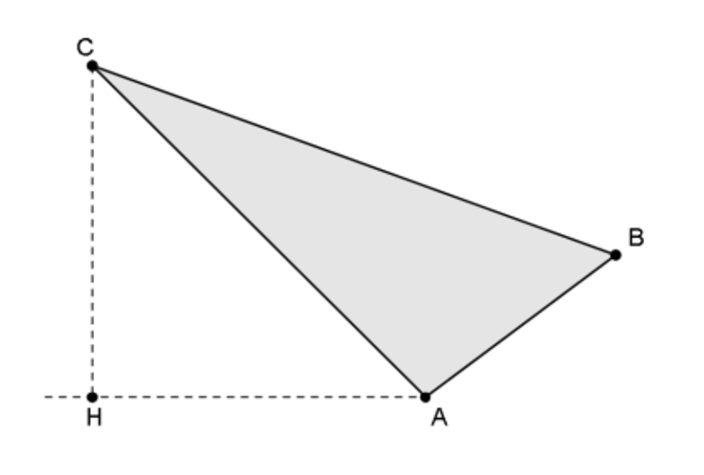
\includegraphics[width=5cm]{triangle}
  \end{center}
  \begin{correction}
    On a les relations suivantes (le point d'interrogation dénote une quantitée non donnée dans l'énoncé) :
    \begin{align*}
      \sin(\widehat{CAH}) &= CH?/CA?  &&\text{(sinus dans un triangle rectangle)}\\
      \sin(B) / CA? &= \sin(C?)/AB &&\text{(loi des sinus)}\\
      C? &= 180-A-B &&\text{(somme des angles d'un triangle)}
    \end{align*}
    Dès lors:
    \begin{equation*}
      \begin{split}
        CH? &= \sin(\widehat{CAH}) \sin(B) AB/\sin(\ang{180}-A-B)\\
        &= \sin(\ang{42}) \sin(\ang{36}) \SI{300}{m} / \sin(\ang{39})\\
        &= \SI{187.49}{m}
      \end{split}
    \end{equation*}
\end{correction}
\end{exo}

\begin{exo}
 Des naufragés abordent les côtes d'une île
  de l'Atlantique Sud, balayées par le vent. La plage est bien dégagée et recouverte de
  galets, mais une falaise barre le chemin vers l'intérieur de l'île
  où ils espèrent trouver du secours.  Avant de se préparer pour
  l'escalade de cette falaise, un membre de l'équipage se propose d'en
  mesurer la hauteur. Pour cela, il plante une perche bien droite de 3
  m de longueur, à une distance de \SI{150}{\metre} de l'aplomb de la falaise.
  Ainsi fait, après avoir vérifié que la perche est bien
  perpendiculaire au plan de l'horizon, il recule de 5m, distance
  juste nécessaire pour que, couché sur le sol, le rayon visuel parti
  de son oeil effleure à la fois l'extrémité de la perche et le sommet
  de la falaise.  Dessiner une figure, puis calculer la valeur trouvée
  pour la hauteur de la falaise.
  \begin{correction}
    \SI{93}{m}
\end{correction}
\end{exo}

\begin{exo}
  Deux édifices à toit plat sont distants de $\SI{60}{m}$. Du toit
  du plus petit édifice, qui a \SI{40}{m} de hauteur, l'angle
  d'élévation de l'arête du toît du plus grand édifice est de
  \ang{40}. Calculer la hauteur du plus grand édifice.
  \begin{center}
    \input{batiment.pdf_t}
  \end{center}
  \begin{correction}
    \SI{90,35}{m}
\end{correction}
\end{exo}

\begin{exo}\ChoisirPourSeance{2015-2016}{geol=3,geog=3,irbi=3,chim=3,scie=3,biol=3,info=3}
  À l'aide du cercle trigonométrique, déterminer les nombres
  suivants (valeur exacte) en utilisant les symétries adéquates.
  \begin{multicols}{3}
    \begin{enumerate}
    \item $\cos\paren*{\frac{5\pi}{6}}$
    \item $\sin\paren*{\frac{-\pi}{4}}$
    \item $\cos\paren*{\frac{3\pi}{4}}$
    \item $\sin\paren*{\frac{-\pi}{2}}$
    \item $\cos\paren*{\frac{7\pi}{3}}$
    \item $\sin\paren*{\frac{-4\pi}{3}}$
    \item $\cos\paren*{\frac{5\pi}{4}}$
    \item $\cos\paren*{\frac{-7\pi}{6}}$
    \item $\sin\paren*{\frac{8\pi}{3}}$
    \end{enumerate}
  \end{multicols}
  \begin{correction}
    \begin{multicols}{3}
      \begin{enumerate}
      \item $-\frac{\sqrt{3}}{2}$
      \item $-\frac{\sqrt{2}}{2}$
      \item $-\frac{\sqrt{2}}{2}$
      \item $-1$
      \item $\frac{1}{2}$
      \item $\frac{\sqrt{3}}{2}$
      \item $-\frac{\sqrt{2}}{2}$
      \item $-\frac{\sqrt{3}}{2}$
      \item $\frac{\sqrt{3}}{2}$
      \end{enumerate}
    \end{multicols}
\end{correction}
\end{exo}

\begin{exo}\ChoisirPourSeance{2015-2016}{geol=3,geog=3,irbi=3,chim=3,scie=3,biol=3,info=3}
  Déterminer les valeurs exactes des expressions suivantes :
  \(\arccos(\frac{\sqrt{3}}{2})\),
  \(\arcsin(\frac{\sqrt{3}}{2})\),
  \(\arctan(1)\).
\begin{correction}
$\pi/6$,  $\pi/3$, $\pi/4$.
\end{correction}
\end{exo}

\begin{exo}\ChoisirPourSeance{2015-2016}{geol=3,geog=3,irbi=3,chim=3,scie=3,biol=3,info=3}
  Simplifier l'expression \(\cos(\arcsin(x))\).
\begin{correction}
  $\arcsin$ prend ses valeurs dans \(\intercc{-\pi/2, \pi/2}\). Le cosinus y est toujours positif, dès lors
\begin{equation*}
  \cos(\arcsin(x)) = \sqrt{1 - \sin^{2}(\arcsin(x))} = \sqrt{1 - x^{2}}
\end{equation*}
pour \(x \in \intercc{-1,1}\)
\end{correction}
\end{exo}


\begin{exo}
Trouver les valeurs exactes possibles de $\cos\theta$ et
  $\tan\theta$ sachant que $\sin\theta = \frac{7}{16}$, puis reporter
  les arcs correspondants sur un cercle.
  \begin{correction}
    $\cos\theta = \pm \frac{3\sqrt{23}}{16}$ ; $\tan\theta = \pm \frac{7\sqrt{23}}{69}$
\end{correction}
\end{exo}

\begin{exo}
 Pour calculer la distance $OA$ entre deux points situés sur les
  rives opposées d'un fleuve, on définit le long d'une des rives un
  segment BC de \SI{300}{\metre}, passant par $O$ avec $OA$ perpendiculaire
  à $BC$. En mesurant les angles $\hat B$ et $\hat C$, on trouve
  respectivement \ang{67;20;} et \ang{53;40;} :
  \begin{center}
    \scalebox{0.7}{\input{exo13.pdf_t}}
  \end{center}
  Calculer la valeur des distances $AB$ et $AC$. En déduire ensuite
  celle de la distance $OA$.
  \begin{correction}
    AB = 281, 95 mètres ; AC = 322,96 mètres ; AO = 260,17 mètres
\end{correction}
\end{exo}

\begin{exo}
 Démontrer les relations suivantes~:
  \begin{equation*}
    \begin{split}
      \sin^4(a) - \cos^4(a) &= \sin^2(a) - \cos^2(a)\\
      & = 2 \sin^2(a) -
      1\\
      \tan^2(a) - \tan^2(b) &= \frac1{\cos^2(a)} -
      \frac1{\cos^2(b)}\\
      \frac{\sin ^2(\theta) - \cos^2(\phi)}{\sin ^2(\theta)
        \sin^2(\phi)} &= 1 - \cot^2(\theta) \cot^2(\phi)
    \end{split}
  \end{equation*}
  \begin{correction}
    \begin{enumerate}
    \item $\sin^4(a) - \cos^4(a) = (\sin^2(a) - \cos^2(a)).(\sin^2(a) + \cos^2(a))= (\sin^2(a) - \cos^2(a)) . 1 = \sin^2(a) - \cos^2(a) = \sin^2(a) - (1-\sin^2(a))= 2\sin^2(a)-1$

    \item $ \tan^2(a) - \tan^2(b) = \frac{\sin^2(a)}{\cos^2(a)} - \frac{\sin^2(b)}{\cos^2(b)} = \frac{1 - \cos^2(a)}{\cos^2(a)} - \frac{1-\cos^2(b)}{\cos^2(b)} = \frac{1}{\cos^2(a)} - 1 - \frac{1}{\cos^2(b)} + 1 = \frac{1}{\cos^2(a)} - \frac{1}{\cos^2(b)} $

    \item $ 1 - \cot^2(\theta) \cot^2(\phi) = 1 - \frac{\cos^2(\theta)}{\sin^2(\theta)} \frac{\cos^2(\phi)}{\sin^2(\phi)} = \frac{\sin^2(\theta)\sin^2(\phi) - \cos^2(\theta)\cos^2(\phi)}{\sin^2(\theta)\sin^2(\phi)} = \frac{\sin^2(\theta)(1 - \cos^2(\phi)) - (1 - \sin^2(\theta))\cos^2(\phi)}{\sin^2(\theta)\sin^2(\phi)} = \frac{\sin^2(\theta) - \sin^2(\theta)\cos^2(\phi) - \cos^2(\phi) + \sin^2(\theta)\cos^2(\phi)}{\sin^2(\theta)\sin^2(\phi)} = \frac{\sin^2(\theta) - \cos^2(\phi) }{\sin^2(\theta)\sin^2(\phi)}$
    \end{enumerate}
\end{correction}
\end{exo}

\begin{exo}Soit $x \in \left[ -\frac\pi2, \frac\pi2 \right]$.
  \begin{enumerate}
  \item Si $\sin x = -\frac{1}{5}$, que vaut la tangente de $x$ ?
  \item Si $\cos x = \frac{1}{3}$, quelles sont les valeurs possibles
    de la tangente de $x$ ?
  \end{enumerate}
  \begin{correction}
    \begin{enumerate}
    \item $-\frac{\sqrt{6}}{12}$
    \item $\pm2\sqrt{2}$
    \end{enumerate}
\end{correction}
\end{exo}

\begin{exo}
 Représenter les graphes des fonctions $l$ et $f$ définies par
  $l(t) = \sin(2t+\pi)$ et $f(t) = \sin(2t) + \pi$.
  \begin{correction}
    ~
  \begin{equation*}
    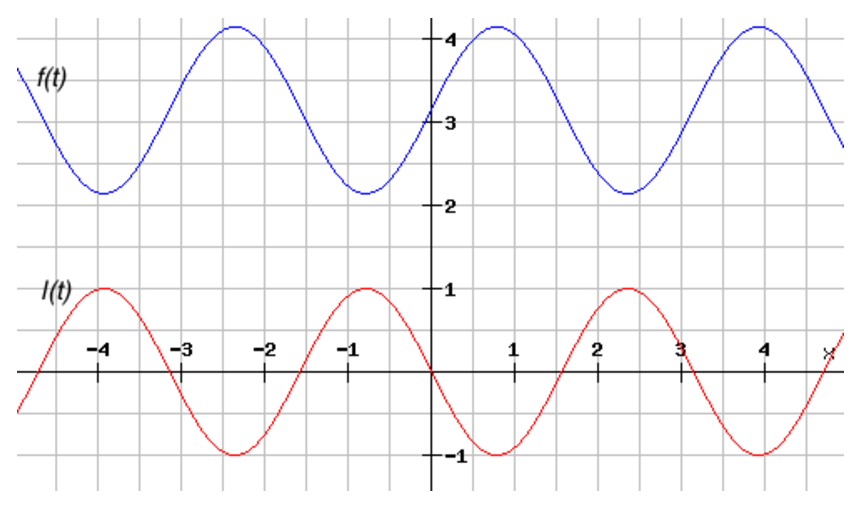
\includegraphics[scale=0.7]{fcttrigo}
  \end{equation*}
\end{correction}
\end{exo}

%% Exercices supprimés
% \begin{exo}
% Deux villes sont vues depuis le centre de la Terre sous un angle
%   de un degré
%   \begin{enumerate}
%   \item Quelle est la distance qui sépare ces deux villes ?
%   \item Quelle serait cette distance si l'angle était de un radian ?
%   \end{enumerate}

%   Le rayon terrestre vaut environ \SI{6370}{km}, et on mesure les
%   distances sans creuser de souterrains.
% Réponse: a) 111,18... km b) 6370 km - question supprimée
% \end{exo}

% \begin{exo}
% Calculer la hauteur d'un phare pour que sa portée soit de \SI{15}{km}.\todo{Need rayon terrestre, faut-il le dire ?}
% Réponse : 17,66 mètres - question supprimée
% \end{exo}
% \begin{exo}
% \todo{ pour l'exo de la tour de Pise, n'est-il pas plus logique
%     que les 54.5m soient la hauteur physique de la tour et pas la
%     projection sur la verticale ??? (Michel AM) -- cela ne changerait
%     pas grand chose (Nicolas R)} La construction de la tour de
%   Pise a commencé en $1173$ et fut achevée en $1350$, avec
%   l'installation de ses sept cloches. C'est une tour creuse, d'un
%   diamètre intérieur de \SI{7,5}{m} et d'une hauteur $h$ de
%   \SI{54,5}{m}. Dès la construction du troisième étage en $1274$,
%   l'édifice commence à pencher, à tel point qu'elle est fermée au
%   public en $1990$.

%   \scalebox{0.55}{\input{pise.pdf_t}}

%   Des travaux très importants sont alors réalisés, qui ont permis de
%   rapprocher le sommet de la verticale de \SI{43}{cm}. Ainsi, la tour de
%   Pise a retrouvé l'inclinaison qu'elle avait il y a deux siècles et
%   peut réouvrir ses portes au public en 2001. Les scientifiques
%   estiment avoir prolongé la survie du monument d'une centaine
%   d'années.  Il s'agit de déterminer l'inclination qu'avait la tour en
%   1990. Pour ce faire, elle est observée à partir d'un point distant
%   de \SI{46}{m} du centre de sa base, et la mesure de l'angle
%   d'élévation est de \ang{53}.

%   Calculer :
%   \begin{itemize}
%   \item La valeur de l'angle d'inclinaison, par rapport à la verticale
%     $\theta$ ;
%   \item La distance $d$, qui exprime de combien de mètres, le centre
%     du sommet de la tour s'était écarté de la verticale.
%   \end{itemize}
% Réponse :  Aujourd'hui : $\theta = 6,88° ; d = 6,54 cm$. En 1990 : $\theta = 7,33° ; d = 6,97 cm$
% \end{exo}
\chapter{Limites, asymptotes et continuité}\requires{chapter:Limites}
\begin{exo}
  Considérons la fonction $f(x) = (x^3 - 1)/(x-1)$ sur le domaine $\RR\setminus\{1\}$.

  Deviner (par exemple avec une calculatrice) vers quoi tend, intuitivement, \(f(x)\) lorsque \(x\) s'approche de \(1\).
   
  Afin de tenter de justifier, montrer que $f(x) = x^2 + x + 1$ pour \(x\) différent de \(1\).
\end{exo}
\begin{exo}\label{limite intuitive sinus x sur x}
  Considérons la fonction $f(x) = \sin(x)/x$ (sur le domaine $\RR_0$).

  Deviner (par exemple avec une calculatrice) vers quoi tend, intuitivement, \(f(x)\) lorsque \(x\) s'approche de \(0\).
   
  Afin de tenter de justifier cela : lorsque \(x\) est proche de \(0\) mais positif, justifier les inégalités \(\sin(x) \leq x \leq \tan(x)\) par un dessin dans le cercle trigonométrique, et en déduire \(\cos(x) \leq f(x) \leq 1\) pour tout \(x\) proche de \(0\) (positif et négatif).
\end{exo}

\begin{exo}
  Considérons la fonction $g(x) = (1 - \cos(x))/x$ (sur le domaine $\mathbb R_0$).

  Deviner (par exemple avec une calculatrice) vers quoi tend, intuitivement, \(g(x)\) lorsque \(x\) s'approche de \(0\).
   
  Afin de tenter de justifier cela, montrer que $g(x) = \tan(x/2) f(x)$ et utiliser l'inégalité montrée à l'exercice \ref{limite intuitive sinus x sur x}.
\end{exo}

%%EXE II.9
\begin{exo}
  Calculer les limites suivantes~:
  \begin{equation*}
    \begin{array}{ll}
      \mbox{a) }\displaystyle{\lim_{x \rightarrow 1} (3x^2+1)};
      &\mbox{b) }\displaystyle{\lim_{x \rightarrow -2}\frac{2x^3+3x-4}{x^2+x-1}}; \\
      & \\
      \mbox{c) }\displaystyle{\lim_{x \rightarrow 1}\frac{x^2-1}{x-1}}; 
      &\mbox{d) }\displaystyle{\lim_{x \rightarrow 2} \frac{x^3-8}{x-2}}; \\
      & \\
      \mbox{e) }\displaystyle{\lim_{h \rightarrow 0} \frac{(1+h)^2-1}{h}}; \quad 
      &\mbox{f) }\displaystyle{\lim_{u \rightarrow u_0} \frac{u^2-u_0^2}{u-u_0}}; \\
      & \\
      \mbox{g) }\displaystyle{\lim_{x \rightarrow 0} \frac{\sqrt{x+4}-2}{x}}; 
      &\mbox{h) }\displaystyle{\lim_{x \rightarrow 4} \frac{\sqrt{2x+1}-3}{x-4}}.
    \end{array}
  \end{equation*}
\end{exo}

\begin{exo}
Calculer les limites à gauche et à droite en 0 de 
 \begin{equation*}
 \mbox{a) } 2x+ \frac{\vert x \vert}{x}; \qquad \mbox{b) } e^{1/x}; 
 \qquad \mbox{c) } \frac{\vert x \vert e^{\vert x \vert}}{x}.
\end{equation*}
\end{exo}
\begin{exo}
Montrer que
 \begin{equation*}
 \lim_{x \rightarrow a} \frac{x^n-a^n}{x-a}=na^{n-1}, \quad 
 \mbox{ pour }n \mbox{ entier }\neq 0 \mbox{ et } a\mbox{ réel }>0.
\end{equation*}
\end{exo}

%%EXE II.6
\begin{exo}
Calculer pour $x$ tendant vers $\displaystyle{\frac{7}{2}}$ 
 les limites à gauche 
 et à droite de 
 \begin{equation*}
 \frac{\vert 2x-7 \vert}{2x-7}.
\end{equation*}
\end{exo}

%%EXE II.7
\begin{exo}
Calculer les limites à gauche et à droite en $\displaystyle{\frac{\pi}
 {2}}$ de
 \begin{equation*}
 \frac{1}{2+2^{tg \, x}}.
\end{equation*}
\end{exo}

%%EXE II.8
\begin{exo}
Si $f$ est une fonction continue et croissante sur l'intervalle $]a,b[$, que peut-on dire des fonctions suivantes aussi sur  $]a,b[$ ?
 \begin{equation*}
 \begin{array}{ll}
 \mbox{a) } x \mapsto -f(x); \qquad &\mbox{ b) } x \mapsto (f(x))^2; \\
 & \\
 \mbox{c) } x \mapsto f(x+c); \qquad &\mbox{ d) } x \mapsto \displaystyle{
 \frac{1}{f(x)}}.
 \end{array}
\end{equation*}
\end{exo}

%%EXE II.10
\begin{exo}
Calculer les limites pour $x \rightarrow + \infty$ et pour 
 $x \rightarrow - \infty$ des fonctions $y=y(x)$ suivantes~:
 \begin{equation*}
 \begin{array}{ll}
 \mbox{a) } y=5x^6+3x^3-7x^2+15; \qquad
 &\mbox{g) } y=\displaystyle{\frac{\sqrt{x^2+x}}{2x+1}}; \\
 & \\
 \mbox{b) } y=2x^5+3x^4-6x^2+x;
 &\mbox{h) } y=\displaystyle{\frac{3 \sqrt{8x^3-1}}{x+4}}; \\
 & \\
 \mbox{c) } y=\displaystyle{\frac{x^3-27}{x^2-9}}; 
 &\mbox{i) } y=\displaystyle{\frac{\sqrt{x+4}-2}{x}}; \\
 & \\
 \mbox{d) } y=\displaystyle{\frac{x-4}{x^2-6x+8}};
 &\mbox{j) } y=\sqrt{2x^2-3x-5}- \sqrt{2x^2+3x-5}; \\
 & \\
 \mbox{e) } y=\displaystyle{\frac{x^2+3x-10}{2(x^2+x-20)}};
 &\mbox{k) } y=x(\sqrt{x^2+1}-x); \\
 & \\
 \mbox{f) } y=\displaystyle{\frac{x^3-3x+1}{2x^3-6x+x}};
 &\mbox{l) } y=\displaystyle{\frac{\sqrt{x^2+1}}{\sqrt[3]{x^3+1}}}.
 \end{array}
\end{equation*}
\end{exo}

%%EXE II.11
\begin{exo}
Sachant que $\limite x 0 \frac{\sin x}{x}=1$, que valent les limites pour $x \rightarrow 0$ des quantités
 \begin{equation*}
 \begin{array}{ll}
 \mbox{a) } \frac{\mbox{tg}\, x}{x}; 
 &\mbox{d) } \frac{x+\sin 4x}{2x- \sin 7x}; \\
 &\\
 \mbox{b) } \frac{\sin 7x}{3x}; 
 &\mbox{e) } \frac{\sqrt{3- \sin 2x}- \sqrt{3+ \sin 2x}}{x}; \\
 & \\
 \mbox{c) } \frac{x \sin x}{1- \cos x}; 
 &\mbox{f) } \sqrt{\frac{\sin 2x}{x}}.
 \end{array}
\end{equation*}
\end{exo}

%%EXE II.12
\begin{exo}
Trouver les asymptotes aux graphes des fonctions $y=y(x)$ suivantes~:
 \begin{equation*}
 \begin{array}{ll}
 \mbox{a) } \displaystyle{y=x+ \frac{1}{x}}; 
 &\mbox{e) } \displaystyle{y=\frac{3x^2+4}{x}}; \\
 & \\
 \mbox{b) } \displaystyle{y=2x+7+ \frac{1}{x-5}}; \qquad 
 &\mbox{f) } \displaystyle{y=x- \sqrt{x^2+4x}}; \\
 & \\
 \mbox{c) } \displaystyle{y=\frac{1-2x}{3x+4}};
 &\mbox{g) } \displaystyle{y=\sqrt{9x^2-x+4}}; \\
 & \\
 \mbox{d) } \displaystyle{y=\frac{2x}{x^2-5x+4}}; 
 &\mbox{h) } \displaystyle{y=x-2+ \frac{x^2}{x^2+9}}.
 \end{array}
\end{equation*}
\end{exo}
\begin{exo}
Pour chacune des fonctions $y=y(x)$ suivantes~:
 \begin{equation*}
 \begin{array}{ll}
 \mbox{a) } y=e^x;\quad &\mbox{c) } y=x; \\
 &\\
 \mbox{b) } y=\sqrt{x};\quad 
  &\mbox{d) } y=\displaystyle{\sqrt{\frac{2x+1}{3(x-1)}}},
 \end{array}
\end{equation*}
 déterminer le plus grand domaine et la fonction réciproque 
 si elle existe. Représenter la fonction, sa fonction réciproque 
 et la première bissectrice sur le même graphique.
\end{exo}
\begin{exo}\ChoisirPourSeance{2014-2015}{phar=2,geol=2,geog=2,irbi=2,chim=2,scie=2,biol=2,info=2,(a,b,c)}
Soit la fonction $f$ donnée par 
 \begin{equation*}
 f(x)=
 \left\{
 \begin{array}{cl}
 \displaystyle{\frac{1}{x}} \quad &\mbox{pour } x < 0, \\
 & \\
 x^2 &\mbox{pour } 0 \leq x \leq 2, \\
 & \\
 x+4 &\mbox{pour } 2<x.
 \end{array}
 \right.
\end{equation*}
 \begin{enumerate}
 \item Calculer $f(-2)$, $f(0)$, $\displaystyle{f\paren*{\frac{3}{2}}}$, 
 $f(3)$. 
 \item Tracer le graphe de $f$.
 \item Déterminer le plus grand domaine de définition et l'image de $f$.
 \item Calculer les limites à gauche et à droite de $f$ en 0, en 1 et en 2.
 \item En quels points $f$ est-elle continue ?
 \end{enumerate}
\end{exo}
\begin{exo}\ChoisirPourSeance{2014-2015}{geol=9,geog=9,irbi=9,chim=9,scie=9,biol=9,info=9}
Soit la fonction $f$ donnée par 
 \begin{equation*}
 f(x)=
 \left\{
 \begin{array}{cl}
 \sqrt{1-x} &\mbox{ pour } x < 1, \\
 & \\
 3 &\mbox{ pour } x=1, \\
 & \\
 \displaystyle{\frac{1}{2} x+1} &\mbox{ pour } 1<x \leq2, \\
 & \\
 2-(x-2)^2 &\mbox{ pour } 2<x.
 \end{array}
 \right.
\end{equation*}
 \begin{enumerate}
 \item Calculer $f(-2)$, $f(0)$, $\displaystyle{f\paren*{\frac{3}{2}}}$, 
 $f(3)$. 
 \item Tracer le graphe de $f$.
 \item Déterminer le plus grand domaine de définition et l'image de $f$.
 \item Calculer les limites à gauche et à droite de $f$ en 0, en 1 et en 2.
 \item En quels points $f$ est-elle continue ?
 \end{enumerate}
\end{exo}
\begin{exo}
  Formulez en termes de $\varepsilon > 0$ une condition nécessaire et suffisante pour que
  \begin{enumerate}
  \item la droite d'équation $x=a$ soit asymptote verticale au graphe de $f$;
  \item la droite d'équation $y=b$ soit asymptote horizontale au graphe de $f$.
  \end{enumerate}
\end{exo}

\begin{exo}
Montrer en termes de $\varepsilon$ et $\delta$ que si les fonctions 
 $f : {\BB R} \rightarrow {\BB R}$ et $g: {\BB R} \rightarrow {\BB R}$ sont continues, 
 il en va de même de la fonction $f \cdot g : {\BB R} \rightarrow {\BB R}$. 
 À cette fin, utilisez
 \begin{equation*}
 (f \cdot g)(x)-(f \cdot g)(x_0)=(f(x)-f(x_0))g(x)+f(x_0)(g(x)-g(x_0)).
\end{equation*}
 Déduisez une nouvelle preuve de la continuité de l'application ${\BB R} \rightarrow
 {\BB R} : x \mapsto x^2$ (c'est-à-dire, un choix de $\delta$ différent de celui proposé 
 dans l'exemple 2 de la section 6.4).
\end{exo}
\begin{exo}\ChoisirPourSeance{2014-2015}{geol=9,geog=9,irbi=9,chim=9,scie=9,biol=9,info=9,(sans,utiliser,de,dérivée)}
Considérons la fonction
 \begin{equation*}
 {\BB R} \rightarrow {\BB R} : x \mapsto \lceil x \rceil - \sqrt{x}.
\end{equation*}
 \begin{enumerate}
 \item En quels points de ${\BB R}$ cette fonction est-elle continue ?
 \item Étudier la croissance de cette fonction.
 \end{enumerate}
\end{exo}
\begin{exo}\ChoisirPourSeance{2014-2015}{geol=9,geog=9,irbi=9,chim=9,scie=9,biol=9,info=9}
  Parmi les fonctions suivantes de ${\BB N}$ vers ${\BB R}^+$, lesquelles sont asymptotiquement du même ordre que la fonction $f : {\BB N} \rightarrow {\BB R}^+ : n \mapsto n^{3/2}$~?
  \begin{equation*}
    \begin{array}{l@{\qquad}l}
      f_1 : n \mapsto 3n^2+2; & f_2 : n \mapsto \sqrt{n^5+6}; \\
                              & \\
      f_3 : n \mapsto \sqrt[3]{n^2+7}; & f_4 : n \mapsto \sqrt{n^3+1}; \\
                              &\\
      f_5 : n \mapsto {\paren*{\frac{3}{2}}}^n; & f_6 : n \mapsto \sqrt[3]{n^2}+(-1)^n; \\
                              &\\
      f_7 : n \mapsto 1; & f_8 : n \mapsto \sqrt[3]{n^2}(1+ \sin n).
    \end{array}
  \end{equation*}
\end{exo}

\begin{exo}\ChoisirPourSeance{2014-2015}{geol=9,geog=9,irbi=9,chim=9,scie=9,biol=9,info=9}
Si deux fonctions $f : {\BB N} \rightarrow {\BB R}$ et $g : {\BB N} \rightarrow {\BB R}$ 
 sont asymptotiquement du même ordre, la limite
 \begin{equation*}
 \lim_{n \rightarrow \infty} \frac{\vert f(n) \vert}{\vert g(n) \vert}
\end{equation*}
 existe-t-elle nécessairement ?
\end{exo}
\begin{exo}
  Voici des fonctions de ${\BB N}$ vers ${\BB R}$, appliquant $n$ sur
  \begin{equation*}
    \begin{array}{ll}
      f_1(n)=\sqrt{n}, &f_2(n)=2n^2+1, \\
                       & \\
      f_3(n)=7n+8, &f_4(n)=2n^3+5, \\
                       & \\
      f_5(n)=\displaystyle{\frac{1}{2} \sqrt{n} -8}, \qquad &f_6(n)=3n+2.
    \end{array}
  \end{equation*}
  Trouvez toutes les comparaisons du type \og $f$ est $O(g)$\fg{} entre ces 
  fonctions. Montrez que ces fonctions peuvent être rangées par ordre asymptotique
  de grandeur.
\end{exo}

\begin{exo}
  Soit $f$ et $g$ deux fonctions de ${\BB N}$ vers ${\BB R}^+$. Si
  \begin{equation*}
    \lim_{n \rightarrow \infty} \frac{f(n)}{g(n)}=0,
  \end{equation*}
  est-il possible que
  \begin{enumerate}
  \item $f$ soit $O(g)$~?
  \item $g$ soit $O(f)$~?
  \end{enumerate}
\end{exo}

\chapter{Fonctions trigonométriques}\requires{chapter:Fonctions trigonométriques}

%%EXE II.19
\begin{exo}
Résoudre les équations suivantes en $x$ :
  
\begin{tabular}{ll}
  a) $\displaystyle{2\sin x-1=0}$;\qquad\qquad         & f) $\displaystyle{\sin 2x-\cos 2x=1}$;            \\[2mm]
  b) $\displaystyle{\sin x-\sin 2x=0}$;\qquad\qquad    & g) $\displaystyle{\sin x=\sqrt 3\cos x}$;         \\[2mm]
  c) $\displaystyle{\sin^2x+\sin x-2=0}$;\qquad\qquad  & h) $\displaystyle{\sin x+\sqrt 3\cos x=\sqrt 2}$; \\[2mm]
  d) $\displaystyle{\sin^22x-\sin^2x=0}$;\qquad\qquad  & i) $\displaystyle{\arccos 2x=\arcsin x}$;         \\[2mm]
  e) $\displaystyle{2\sin^2x-\sin x-1=0}$;\qquad\qquad & j) $\displaystyle{\arccos(2x^2-1)=2\arccos\frac{1}{2}}$.
\end{tabular}
\end{exo}
\begin{exo}
Déterminer la valeur de chacune des expressions suivantes :
  
  \begin{tabular}{ll}
  a) $\displaystyle{\arcsin\frac{\sqrt 2}{2}}$;\qquad\qquad&
  f) $\displaystyle{\sin(\arccos\frac{\sqrt 3}{2})}$;\\[2mm]
  b) $\displaystyle{\arccos\frac{1}{2}}$;\qquad\qquad&
  g) $\displaystyle{\cos(\arcsin\frac{\sqrt 2}{2})}$;\\[2mm]
  c) $\displaystyle{\arctg 1}$;\qquad\qquad&
  h) $\displaystyle{\coseca(\arcsin\frac{1}{2})}$;\\[2mm]
  d) $\displaystyle{\arccotg(-1)}$;\qquad\qquad&
  i) $\displaystyle{\cotg(\arctg 1)}$;\\[2mm]
  e) $\displaystyle{}\arccoseca 2$;\qquad\qquad&
  j) $\displaystyle{\seca(\arccotg \sqrt 3)}$.
  \end{tabular}
\end{exo}
\begin{exo}
Déterminer la valeur (en fonction de $x$) de chacune des
  expressions suivantes :
  
  \begin{tabular}{ll}
  a) $\displaystyle{\sin(2\arccos x)}$;\qquad\qquad&
  d) $\displaystyle{\sin(2\arccos 4x)}$;\\[2mm]
  b) $\displaystyle{\cotg(\arccos x)}$;\qquad\qquad&
  e) $\displaystyle{\sin(\arctg x)}$;\\[2mm]
  c) $\displaystyle{\cos(2\arcsin x)}$;\qquad\qquad&
  f) $\displaystyle{\tg(\arcsin 5x)}$.
  \end{tabular}
\end{exo}
\begin{exo}
Déterminer les domaines de définition des fonctions
  $x\mapsto y=y(x)$ suivantes :
  
  \begin{tabular}{ll}
  a) $\displaystyle{\arccotg 3x}$;\qquad\qquad&
  e) $\displaystyle{y=\sin(\arccos\frac{x}{3})}$;\\[2mm]
  b) $\displaystyle{y=\arcsin 5x}$;\qquad\qquad&
  f) $\displaystyle{y=\arccos\frac{2x}{x+1}}$;\\[2mm]
  c) $\displaystyle{y=\arctg(\sin 3x)}$;\qquad\qquad&
  g) $\displaystyle{y=\arccos(\tg 2x)}$;\\[2mm]
  d) $\displaystyle{y=\arccos\frac{3x}{x-2}}$;\qquad\qquad&
  h) $\displaystyle{y=\arcsin(\cotg 3x)}$.
  \end{tabular}
\end{exo}
\begin{exo}
Pour chacune des fonctions $y$ de $x$ suivantes déterminer
  un domaine où celle-ci est inversible, et donner la fonction
  réciproque correspondante.
  
  \begin{tabular}{ll}
  a) $\displaystyle{y=1+2\sin x}$;\qquad\qquad&
  d) $\displaystyle{y=\arcsin(2x+1)}$;\\[2mm]
  b) $\displaystyle{y=1+\sin 2x}$;\qquad\qquad&
  e) $\displaystyle{y=\cos^2x-\sin x}$.\\[2mm]
  c) $\displaystyle{y=\tg^2x}$;&
  \end{tabular}
\end{exo}

%%EXE II(fonctions élémentaires).1
\begin{exo}
Calculer les dérivées premières des fonctions $y=y(x)$
  suivantes (où $a, b\in\BB R$) :\\
  
  \begin{tabular}{ll}
  a) $\displaystyle{y=\sin(x^2+1)}$;\qquad\qquad&
  j) $\displaystyle{y=\tg x-\cotg x}$;\\[3mm]
  b) $\displaystyle{y=\cos\sqrt{1-2x}}$;\qquad\qquad&
  k) $\displaystyle{y=\cos(\sin x)}$;\\[3mm]
  c) $\displaystyle{y=\tg \sqrt x}$;\qquad\qquad&
  l) $\displaystyle{y=\frac{\sin(a-x)}{\sin(a+x)}}$;\\[3mm]
  d) $\displaystyle{y=\coseca x\cotg x}$;\qquad\qquad&
  m) $\displaystyle{y=\arcsin 5x}$;\\[3mm]
  e) $\displaystyle{y=\frac{\sin x+\cos x}{\sin x-\cos
  x}}$;\qquad\qquad& 
  n) $\displaystyle{y=\arccos(\frac{3x}{x-2})}$;\\[3mm]
  f) $\displaystyle{y=\frac{1+\cos 2x}{1-\cos 2x}}$;\qquad\qquad&
  o) $\displaystyle{y=\arctg(\sin 3x)}$;\\[3mm]
  g) $\displaystyle{y=\sin nx\cdot(\sin x)^n}$;\qquad\qquad&
  p) $\displaystyle{y=\arccos\frac{b+a\cos x}{a+b\cos
  x},\quad|a|>|b|}$;\\[3mm] 
  h) $\displaystyle{y=\sqrt{a\sin^2x+b\cos^2 x}}$;\qquad\qquad&
  q) $\displaystyle{y=\sin(\arccos\frac{x}{3})}$.\\[3mm]
  i) $\displaystyle{y=\coseca^4x}$;&
  \end{tabular}
\end{exo}
\begin{exo}
Calculer les valeurs des dérivées première, deuxième
  et troisième des fonctions $y=y(x)$ suivantes aux points
  indiqués :\\
  \begin{tabular}{ll}
  a) $\displaystyle{y=\sin x\cos x}$,\qquad\qquad&
  pour \quad $\displaystyle{x=\frac{\pi}{3}}$;\\[3mm]
  b) $\displaystyle{y=4\sin x-3\cos x}$,\qquad\qquad&pour
  \quad$\displaystyle{x=0}$;\\[3mm]
  c) $\displaystyle{y=\sin 3x\cos x}$,\qquad\qquad&pour
  \quad$\displaystyle{x=\frac{\pi}{4}}$.
  \end{tabular}
\end{exo}  
\begin{exo}
Prouver que la dérivée d'ordre $n\geq 3$ de la fonction
 $x\mapsto y=\arctg x$ satisfait la formule de récurrence
 $$
 \displaystyle{y^{n/}=\frac{-2(n-1)xy^{n-1/}-(n-1)(n-2)y^{n-2/}}{1+x^2}}
 $$
Calculer la valeur de la cinquième
 dérivée de $\arctg x$ au point $x=1$.
\end{exo}

%%EXE II.17
\begin{exo}\ChoisirPourSeance{2014-2015}{geol=5,geog=5,irbi=5,chim=5,scie=5,biol=5,info=5}
Tracer le graphe de la fonction $x\mapsto y=\sin x$. Déduire
  les graphiques des courbes $y=\sin 2x,\quad
  y=\displaystyle{\frac{1}{2}}\sin 2x$.
\end{exo}

\chapter{Fonctions logarithmes}\requires{chapter:Fonctions logarithmes}

%%EXE II(fonctions élémentaires).6
\begin{exo}\ChoisirPourSeance{2014-2015}{phar=3,geol=5,geog=5,irbi=5,chim=5,scie=5,biol=5,info=5}
  Calculer sans faire usage de tables ou de machines :
  \begin{multicols}{2}
    \begin{enumerate}\everymath{\displaystyle}
    \item $\log_2(32)$;          
    \item $\log_3(27)$;          
    \item $\log_{10}(0,0000001)$;
    \item $\log_5(125)$;         
    \item $\log_8(16)$;          
    \item $\log_{1/2}(4)$;
    \item $\ln (e^{-7})$;
    \item $\log_{10} (10^4)$;
    \item $\log_{\sqrt{32}}(32)$;
    \item $\log_{16}(8)$.                
    \end{enumerate}
  \end{multicols}
\end{exo}

%%EXE II(fonctions élémentaires).7
\begin{exo}\ChoisirPourSeance{2014-2015}{phar=3,geol=5,geog=5,irbi=5,chim=5,scie=5,biol=5,info=5}
Sachant que $\log_{10}\,2\approx 0{,}30103\ldots$, évaluer le
  nombre de chiffres de $2^{56}$.
\end{exo}

%%EXE II(fonctions élémentaires).8
\begin{exo}\ChoisirPourSeance{2014-2015}{phar=3,geol=5,geog=5,irbi=5,chim=5,scie=5,biol=5,info=5}
Calculer $x$ tel que
  
  \begin{tabular}{ll}
  a) $\displaystyle{\log_x\,5=0{,}5}$;\qquad\qquad&
  d) $\displaystyle{\log_x\,a=a\quad(a>0\mbox{ et }a\neq 1)}$;\\[3mm]
  b) $\displaystyle{\log_x\,8=-1{,}5}$;\qquad\qquad&
  e) $\displaystyle{\log_x\,a=-a}\quad(a>0\mbox{ et }a\neq 1)$;\\[3mm]
  c) $\displaystyle{\log_x\,2=-2}$\qquad\qquad&
  f) $\displaystyle{\log_x\,a=\frac{1}{a}\quad(a>0\mbox{ et }a\neq 1)}$.
  \end{tabular}
\end{exo}
\begin{exo}
Pour quelles valeurs de $a$ et $b$ réels avons-nous
  $\log_a\,b<0$ ?
\end{exo}
\begin{exo}
Démontrer les identités 
  
  a) $\log_b\,a\cdot\log_c\,b\cdot\log_a\,c=1$;\\
  
  b) $\displaystyle{\frac{1}{\log_a\,x}
  +\frac{1}{\log_b\,x}=\frac{1}{\log_{ab}\,x}.}$
\end{exo}
\begin{exo}\ChoisirPourSeance{2014-2015}{phar=3,geol=5,geog=5,irbi=5,chim=5,scie=5,biol=5,info=5}
Calculer en fonction de $a=\log_{10}\,2$ :\\
  
  a) $\log_{10}\,5$;\qquad b) $\log_{10}\,125$;\qquad c)
  $\log_{10}\,2{,}5$.

\begin{correction}
  1 - a ; 3 - 3a ; 1 - 2a
\end{correction}
\end{exo}

%%EXE II(fonctions élémentaires).9
\begin{exo}
Le logarithme d'un nombre vaut 3 dans une certaine base. Ce
  logarithme vaut 4 si l'on double la base. Quel est ce nombre ?
  Quelle est cette base ?

\begin{correction}
  On écrit : $a^3 = x = (2a)^4 = 16 a^4$, dont on tire la base $a = 1/4096$, et le nombre $x= 1/16$.
\end{correction}
\end{exo}
\begin{exo}
Pour quelle valeur de $x$ la quantité $\log_x\,5$ est-elle
  d'une unité plus grande que $\log_x\,4$~?
\end{exo}
\begin{exo}
Simplifier l'expression $\log_a\,(\log_a\,a^{a^x})$.
\end{exo}

%%EXE II(fonctions élémentaires).10
\begin{exo}\ChoisirPourSeance{2014-2015}{geol=5,geog=5,irbi=5,chim=5,scie=5,biol=5,info=5}
Résoudre les équations suivantes :\\
  
  a) $\log_3(x+2)+1=\log_3(x^2+4x)$;\\
  
  b) $\log x+\log(x^2+2x-1)=-\log 2$;\\
  
  c) $\log_5(5^x-7)=\log_{25}\,324+2-x$;\\
  
  d) $2\log_2\,x+\log_x\,2=3$;\\
  
  e) $4\log x=\log(x^2-2)+\log 8$;\\
  
  f)
  $\displaystyle{\frac{1}{\log_{3x}\,30x}+\frac{1}{\log_{2x}\,30x}
  +\frac{1}{\log_{x-2}\,30x}=1}$;\\
  
  g) $(\log_4\,x)^2-\log_x\,x+1=0$.
\end{exo}
\begin{exo}
Trouver toutes les solutions du système suivant :
  \begin{equation*}
  \left\{
  \begin{array}{l}
  x^y=10,\\
  2y-\log_{10}\,x=1.
  \end{array}
  \right.
\end{equation*}
  Pour quelle(s) valeur(s) de $a$ avons-nous $x=y$ ?
\end{exo}
\begin{exo}
Résoudre le système
  \begin{equation*}
  \left\{
  \begin{array}{l}
  \log_2 x + \log_2 y=2,\\
  \displaystyle{4x+\frac{y}{100}=5}.
  \end{array}
  \right.
\end{equation*}
\end{exo}

%%EXE II(fonctions élémentaires).11
\begin{exo}
Soit la courbe de $\BB R^2$ d'équation $y=\log_a\,x$.
  
  a) Quelle est la valeur de l'abscisse du point de la courbe où la
  tangente passe par l'origine ?
  
  b) Quelle valeur doit prendre $a$ pour que cette tangente soit
  inclinée à 45$^0$ sur l'axe des $x$ ?
\end{exo}
\begin{exo}
Déterminer les plus grands domaines de définition des
  fonctions $y=y(x)$ suivantes :\\
  a) $\displaystyle{y=\ln \left(\frac{3-2x}{3+2x}\right)}$;\qquad\qquad
  b) $\displaystyle{y=\frac{1-\ln x}{1+\ln x}}$.
\end{exo}

%%EXE II(fonctions élémentaires).2
\begin{exo}
Résoudre les équations exponentielles suivantes :\\
  
  \begin{tabular}{ll}
  a) $\displaystyle{2^x+2^{x+1}=3}$;\qquad\qquad&
  e) $\displaystyle{9^x-2\cdot3^{x+1}=27}$;\\[3mm]
  b) $\displaystyle{3^{2x+1}+9^x=324}$;\qquad\qquad&
  f) $\displaystyle{2^{x+1}+4^x=80}$;\\[3mm]
  c) $\displaystyle{e^x+e^{-x}=2}$;\qquad\qquad&
  g) $\displaystyle{4^x-5\cdot2^x+6=0}$;\\[3mm]
  d) $\displaystyle{(\frac{9}{4})^x-\frac{8}{27}=0}$;\qquad\qquad&
  h) $\displaystyle{2(e^x-e^{-x})=e^x+e^{-x}}$.
  \end{tabular}
\end{exo}

%%EXE II(fonctions élémentaires).3
\begin{exo}
Déterminer les valeurs du paramètre $a$ pour lesquelles
  l'équation
  \begin{equation*}
  e^{2x}-2e^x+a=0
\end{equation*}
  admet des solutions. Pour les valeurs trouvées, résoudre
  l'équation.
\end{exo}
\begin{exo}
Pour quelles valeurs du paramètre $m$ le système
  \begin{equation*}
  \left\{
  \begin{array}{l}
  e^{2x}-7e^x+12=0\\
  e^{2x}-3e^x+m=0
  \end{array}
  \right.
\end{equation*}
  admet-il des solutions ? Quelles sont les solutions correspondantes
  ?
\end{exo}
\begin{exo}
Déterminer les coordonnées du point de contact de la
  tangente menée par l'origine au graphe de la fonction $
  x\mapsto y=2^x$.
\end{exo}

%%EXE II(fonctions élémentaires).4
\begin{exo}
Pour quelles valeurs du paramètre $a$ les courbes
  d'équations $y=e^{2x}+1$ et $y=2ae^x$ ont-elles des points
  d'intersection ? Pour quelle(s) valeur(s) de $a$ n'ont-elles qu'un
  seul point d'intersection ? Montrer qu'elles sont alors tangentes
  en ce point et écrire l'équation de la tangente commune.
\end{exo}
\begin{exo}
Calculer la valeur de chacune des fonctions suivantes au point
  indiqué :
  
  \begin{tabular}{ll}
  
  a) $y=2\ch x-\sh x$,\qquad &pour \quad
  $\displaystyle{x=\frac{1}{2}\,\ln 3}$;\\[3mm]
  b) $y=3\ch x-2\sh x$,\qquad &pour \quad
  $\displaystyle{x=\frac{1}{2}\,\ln 2}$;\\[3mm]
  c) $y=\ch 2x+2\sh 2x$,\qquad &pour \quad
  $\displaystyle{x=\frac{1}{2}\,\ln 5}$.
  \end{tabular}
\end{exo}

%%EXE II(fonctions élémentaires).12
\begin{exo}
Calculer les dérivées premières des fonctions $x\mapsto
  y$ suivantes :\\
  
  \begin{tabular}{ll}
  a) $\displaystyle{y=\ln (x^2+1)}$;\qquad\qquad&
  h) $\displaystyle{y=\sh x\,\sin x}$;\\[3mm]
  b) $\displaystyle{y=\ln (\ln x)}$;\qquad\qquad&
  i) $\displaystyle{y=\argsh \sqrt{x+1}}$;\\[3mm]
  c) $\displaystyle{y=\log_5\,\frac{x^2+1}{x^2-1}}$;\qquad\qquad&
  j) $\displaystyle{y=\argth \frac{x}{3}}$;\\[3mm]
  d) $\displaystyle{y=2^{\sqrt x}}$;\qquad\qquad&
  k) $\displaystyle{y=\argch e^{3x}}$;\\[3mm]
  e) $\displaystyle{y=5^{\tg 2x}}$;\qquad\qquad& 
  l) $\displaystyle{y=\frac{1-\ln x}{1+\ln x}}$;\\[3mm]
  f) $\displaystyle{y=x^{1/x}}$;\qquad\qquad& 
  m)
  $\displaystyle{y=\ln [(2x^2+3)^{1/4}(x^3-6)^{1/3}
  (3x^4+7)^{1/2}]}$;\\[3mm]
  g) $\displaystyle{y=x^{\ln x}}$;\qquad\qquad& 
  n) $\displaystyle{y=e^{\frac{1+x}{1-x}}}$.
  \end{tabular}
\end{exo}
\begin{exo}
Vérifier que si $\displaystyle{y=e^{x^2}}$, alors
  \begin{equation*}
  y^{(n)}=2(n-1)y^{(n-2)}+2xy^{(n)}
\end{equation*}
  pour $n>1$. Calculer la cinquième dérivée de
  $\displaystyle{e^{x^2}}$ en $x=1$.
\end{exo}
\begin{exo}
Démontrer les identités suivantes :
  
  a) $\sh(x+y)=\sh x\ch y +
  \ch x\sh y$;
  
  b) $\displaystyle{\ch x-\ch
  y=2\sh\,\frac{x+y}{2}\,\sh\,\frac{x-y}{2}}$;
  
  c) $\ch 2x=\ch^2x+\sh^2x$.
\end{exo}
\begin{exo}
Pour chacune des fonctions suivantes déterminer :
  
  a) son domaine de définition;
  
  b) sa fonction réciproque;
  
  c) le domaine de définition de la fonction réciproque.\\
  \hspace*{10mm} 1$^0$ $y=\ln (\arccos x)$;\\[3mm]
  \hspace*{10mm} 2$^0$ $\displaystyle{y=\arctg
  \frac{e^x+1}{e^x-1}}$;\\[3mm]
  \hspace*{10mm} 3$^0$ $\displaystyle{y=10^{\frac{1-x}{1+x}}}$;\\[3mm]
  \hspace*{10mm} 4$^0$ $\displaystyle{y=e^{\sin 3x}}$;\\[3mm]
  \hspace*{10mm} 5$^0$ $\displaystyle{y=\arccos e^{x+1}}$.
\end{exo}
\begin{exo}
Tracer le graphe de la fonction cosécante. Cette fonction
  est-elle périodique, continue~? Quelle est sa dérivée ?
\end{exo}
\begin{exo}
Considérons la fonction sécante
  appliquant $x$ sur $\displaystyle{\seca x=\frac{1}{\cos
  x}}$.
  
  a) Esquisser son graphe.
  
  b) Déterminer les asymptotes.
  
  c) Proposer une définition de la fonction $x\mapsto
  \arcseca x$. Quel domaine a-t-elle ? Quelle est son image ?
  
  d) Tracer le graphe de la fonction arc sécante.
  
  e) Calculer la dérivée de la fonction arc sécante.
\end{exo}
\begin{exo}
En vue d'étudier des temps d'exécution d'algorithmes, on
  définit parfois la {\em taille} $\alpha$ d'un nombre naturel $m$
  comme étant
  
  \begin{equation*}
  \alpha = 1 + \lceil\log_2(|m|+1)\rceil.
\end{equation*}
  
  a) Que vaut la taille de
  \begin{equation*}
  7~?\qquad\qquad 9~?\qquad\qquad -11~?\qquad\qquad 1~?
  \qquad\qquad-1~?\qquad\qquad 0~?
\end{equation*}
  
  b) Soit deux nombres $m$ et $n$ de tailles respectives $\alpha$ et
  $\beta$. Trouver une {\em \og bonne\fg{}} majoration de la taille du
  produit $mn$.
\end{exo}

%%EXE II(fonctions élémentaires).13
\begin{exo}
Le passage par les logarithmes aide également au calcul des
  dérivées. Par exemple, soit $f(x)=x^x$; de
  \begin{equation*}
  \ln f(x)=x\ln x,
\end{equation*}
  nous déduisons en dérivant par rapport à $x$
  \begin{equation*}
  \frac{f'(x)}{f(x)}=(\ln x)+\frac{x}{x},
\end{equation*}
  donc
  \begin{equation*}
f'(x)=(1+\ln x)f(x)
\end{equation*}
  et
  \begin{equation*}
f'(x)=(1+\ln x)x^x.
\end{equation*}
  En utilisant la même méthode, calculer la dérivée de chacune
  des fonctions $f$ données par
  
  \begin{tabular}{l}
  a) $f(x)=x^r$, avec $r\in\BB R$;\\[2mm]
  
  b) $\displaystyle{f(x)=\sqrt[5]{(x-3)^3(x+1)^2}}$;\\[2mm]
  
  c) $f(x)=f_1(x)\cdot f_2(x)\cdot f_3(x)$, où $f_1, f_2, f_3$ sont
  des fonctions dérivables;\\[2mm]
  
  d) $f(x)=a^x$, avec $a\in\BB R$;\\[2mm]
  
  e) $\displaystyle{f(x)=(\sin x)^{\cos x}}$;\\[2mm]
  
  f) $\displaystyle{f(x)=(\sin x)^{\ln \tg x}}$.
  \end{tabular}
\end{exo}

%%EXE II(fonctions élémentaires).14
\begin{exo}\ChoisirPourSeance{2014-2015}{geol=5,geog=5,irbi=5,chim=5,scie=5,biol=5,info=5}
Le graphique semi-logarithmique d'une fonction $x\mapsto f(x)$
  s'obtient en portant $x$ en abscisse et $\ln f(x)$ en
  ordonnée (lorsque $f(x)>0$).
  
  a) Tracer le graphique semi-logarithmique des fonctions $f_i$
  données pour $i=1,2,3$ par
  \begin{equation*}
  \begin{array}{l}
  \displaystyle{f_1(x)=5e^{3x}};\\[2mm]
  \displaystyle{f_2(x)=e^3\sqrt[5]{x^3}};\\[2mm]
  \displaystyle{f_3(x)=2^x}.
  \end{array}
\end{equation*}
  
  b) Quelles sont les fonctions dont les graphiques
  semi-logarithmiques sont des droites~?
  
  c) Tracer dans un même système d'axes les graphiques
  semi-logarithmiques donnés pour $i=4,5,6$ par
  \begin{equation*}
  \begin{array}{l}
  f_4(x)=5\cdot 3^x;\\[2mm]
  f_5(x)=4^x;\\[2mm]
  f_6(x)=10\cdot 2^x.
  \end{array}
\end{equation*}
  
  d) Si au lieu de porter en ordonnée $\ln f(x)$ on décide
  plutôt de porter $\log_{10}\,f(x)$, comment se modifie le
  graphique semi-logarithmique ?
\end{exo}

%%EXE II(fonctions élémentaires).15
\begin{exo}
Le graphique logarithmique d'une fonction
  $\BB R^+\rightarrow\BB R^+:x\mapsto f(x)$ s'obtient en portant $\ln
  x$ en abscisse et $\ln f(x)$ en ordonnée.
  
  a) Tracer le graphique logarithmique des fonctions $f_i$ données
  pour $i=1,2,3$ par
  \begin{equation*}
  \begin{array}{l}
  \displaystyle{f_1(x)=e^3\sqrt[5]{x^3}};\\[2mm]
  f_2(x)=3^x;\\[2mm]
  \displaystyle{f_3(x)=e^{e^x}}.
  \end{array}
\end{equation*}
  
  b) Quelles sont les fonctions dont les graphiques logarithmiques
  sont des droites ?
  
  c) Tracer dans un même système d'axes les graphiques
  logarithmiques des fonctions $f_1$ données pour $i=4,5,6$ par
  \begin{equation*}
  \begin{array}{l}
  f_4(x)=x^2;\\[2mm]
  f_5(x)=x^{3/2};\\[2mm]
  f_6(x)=10x^{3/2}.
  \end{array}
\end{equation*}
\end{exo}
\begin{exo}
Tracer dans un même système d'axes les graphes des fonctions
  sinus hyperbolique et cosinus hyperbolique. Déterminer les
  asymptotes.
\end{exo}
\begin{exo}
Tracer le graphe de la fonction sinus hyperbolique. Admet-il
  des asymptotes ? La fonction est-elle paire, impaire, périodique ?
\end{exo}
\begin{exo}
Tracer le graphe de la fonction argsh. Admet-il des droites
  asymptotes ? Établissez la formule qui donne la dérivée de la
  fonction argsh.
\end{exo}
\begin{exo}
Pour quelle(s) valeur(s) de $x$ réel avons-nous
  
  a) $\argsh x = \ln\left(x+\sqrt{1+x^2}\right)$?
  
  \vspace{2mm}
  
  b) $\argth x= \displaystyle{\frac{1}{2}\ln\frac{1+x}{1-x}}$?
  
  \vspace{2mm}
  
  c) $\argch x= \ln\left(x+\sqrt{x^2-1}\right)$?
\end{exo}

\chapter{Dérivées}\requires{chapter:Dérivées}

\begin{exo}\ChoisirPourSeance{2014-2015}{geol=10,geog=10,irbi=10,chim=10,scie=10,biol=10,info=10}
 L'abscisse $x$ d'un objet sur un axe est donnée en fonction
 du temps $t$ par le graphe ci-dessous.
 Esquisser le graphe donnant la vitesse de cet objet en fonction du
 temps.
 
\begin{center}
 \psset{xunit=0.60cm,yunit=0.60cm,algebraic=true, dotstyle=o,dotsize=3pt 0,linewidth=0.8pt,arrowsize=3pt 2,arrowinset=0.25}
\begin{pspicture*}(-2,-1.21)(9.31,4.23)
\psaxes[labelFontSize=\scriptstyle,xAxis=true,yAxis=true,labels=none,Dx=2,Dy=2,ticksize=0pt 0,subticks=2]{->}(0,0)(-1.1,-1.21)(9.31,4.23)
\pscustom[linewidth=1.6pt]{\moveto(0.58,2.42)
\lineto(0.59,2.41)
\lineto(0.6,2.41)
\lineto(0.61,2.41)
\lineto(0.62,2.41)
\lineto(0.63,2.41)
\lineto(0.63,2.4)
\lineto(0.64,2.4)
\lineto(0.65,2.4)
\lineto(0.66,2.4)
\lineto(0.67,2.39)
\lineto(0.68,2.39)
\lineto(0.69,2.39)
\lineto(0.7,2.39)
\lineto(0.71,2.38)
\lineto(0.72,2.38)
\lineto(0.73,2.38)
\lineto(0.74,2.37)
\lineto(0.75,2.37)
\lineto(0.76,2.37)
\lineto(0.77,2.36)
\lineto(0.78,2.36)
\lineto(0.79,2.35)
\lineto(0.8,2.35)
\lineto(0.81,2.34)
\lineto(0.82,2.34)
\lineto(0.83,2.34)
\lineto(0.84,2.33)
\lineto(0.84,2.33)
\lineto(0.85,2.32)
\lineto(0.86,2.32)
\lineto(0.87,2.31)
\lineto(0.88,2.31)
\lineto(0.89,2.3)
\lineto(0.9,2.3)
\lineto(0.91,2.29)
\lineto(0.92,2.28)
\lineto(0.93,2.28)
\lineto(0.94,2.27)
\lineto(0.95,2.27)
\lineto(0.97,2.26)
\lineto(0.98,2.25)
\lineto(0.99,2.25)
\lineto(1,2.24)
\lineto(1.01,2.23)
\lineto(1.02,2.23)
\lineto(1.03,2.22)
\lineto(1.04,2.21)
\lineto(1.05,2.21)
\lineto(1.06,2.2)
\lineto(1.07,2.19)
\lineto(1.08,2.19)
\lineto(1.09,2.18)
\lineto(1.1,2.17)
\lineto(1.11,2.16)
\lineto(1.12,2.15)
\lineto(1.13,2.15)
\lineto(1.14,2.14)
\lineto(1.14,2.14)
\lineto(1.14,2.14)
\lineto(1.14,2.14)
\lineto(1.14,2.14)
\lineto(1.14,2.14)
\lineto(1.14,2.14)
\lineto(1.14,2.14)
\lineto(1.14,2.14)
\lineto(1.14,2.14)
\moveto(0,2.24)
\lineto(0,2.24)
\lineto(0,2.24)
\lineto(0,2.24)
\lineto(0,2.24)
\lineto(0,2.24)
\lineto(0,2.24)
\lineto(0,2.24)
\lineto(0,2.24)
\lineto(0,2.24)
\lineto(0,2.24)
\lineto(0,2.24)
\lineto(0,2.24)
\lineto(0,2.24)
\lineto(0,2.24)
\lineto(0,2.24)
\lineto(0,2.24)
\lineto(0,2.24)
\lineto(0,2.24)
\lineto(0.01,2.25)
\lineto(0.02,2.26)
\lineto(0.02,2.26)
\lineto(0.03,2.27)
\lineto(0.04,2.27)
\lineto(0.05,2.28)
\lineto(0.05,2.29)
\lineto(0.06,2.29)
\lineto(0.07,2.3)
\lineto(0.08,2.3)
\lineto(0.08,2.31)
\lineto(0.09,2.31)
\lineto(0.1,2.32)
\lineto(0.11,2.32)
\lineto(0.11,2.33)
\lineto(0.12,2.33)
\lineto(0.13,2.34)
\lineto(0.14,2.34)
\lineto(0.14,2.35)
\lineto(0.15,2.35)
\lineto(0.16,2.35)
\lineto(0.17,2.36)
\lineto(0.18,2.36)
\lineto(0.18,2.37)
\lineto(0.19,2.37)
\lineto(0.2,2.37)
\lineto(0.21,2.38)
\lineto(0.21,2.38)
\lineto(0.22,2.38)
\lineto(0.23,2.39)
\lineto(0.24,2.39)
\lineto(0.25,2.39)
\lineto(0.25,2.4)
\lineto(0.26,2.4)
\lineto(0.27,2.4)
\lineto(0.28,2.4)
\lineto(0.29,2.41)
\lineto(0.3,2.41)
\lineto(0.3,2.41)
\lineto(0.31,2.41)
\lineto(0.32,2.41)
\lineto(0.33,2.42)
\lineto(0.34,2.42)
\lineto(0.35,2.42)
\lineto(0.35,2.42)
\lineto(0.36,2.42)
\lineto(0.37,2.42)
\lineto(0.38,2.42)
\lineto(0.39,2.42)
\lineto(0.4,2.42)
\lineto(0.4,2.43)
\lineto(0.41,2.43)
\lineto(0.42,2.43)
\lineto(0.43,2.43)
\lineto(0.44,2.43)
\lineto(0.45,2.43)
\lineto(0.46,2.43)
\lineto(0.47,2.43)
\lineto(0.47,2.43)
\lineto(0.48,2.43)
\lineto(0.49,2.43)
\lineto(0.5,2.43)
\lineto(0.51,2.43)
\lineto(0.52,2.42)
\lineto(0.53,2.42)
\lineto(0.54,2.42)
\lineto(0.54,2.42)
\lineto(0.55,2.42)
\lineto(0.56,2.42)
\lineto(0.57,2.42)
\lineto(0.58,2.42)
}
\pscustom[linewidth=1.6pt]{\moveto(2.99,1.61)
\lineto(3.02,1.62)
\lineto(3.05,1.62)
\lineto(3.08,1.63)
\lineto(3.11,1.63)
\lineto(3.14,1.64)
\lineto(3.16,1.65)
\lineto(3.19,1.65)
\lineto(3.22,1.66)
\lineto(3.25,1.67)
\lineto(3.28,1.68)
\lineto(3.31,1.68)
\lineto(3.34,1.69)
\lineto(3.37,1.7)
\lineto(3.4,1.71)
\lineto(3.43,1.72)
\lineto(3.46,1.73)
\lineto(3.49,1.74)
\lineto(3.52,1.75)
\lineto(3.55,1.76)
\lineto(3.58,1.78)
\lineto(3.61,1.79)
\lineto(3.64,1.8)
\lineto(3.68,1.81)
\lineto(3.71,1.83)
\lineto(3.74,1.84)
\lineto(3.77,1.85)
\lineto(3.8,1.87)
\lineto(3.83,1.88)
\lineto(3.86,1.9)
\lineto(3.89,1.91)
\lineto(3.92,1.93)
\lineto(3.96,1.94)
\lineto(3.99,1.96)
\lineto(4.02,1.97)
\lineto(4.05,1.99)
\lineto(4.08,2.01)
\lineto(4.11,2.02)
\lineto(4.15,2.04)
\lineto(4.18,2.06)
\lineto(4.21,2.08)
\lineto(4.24,2.1)
\lineto(4.27,2.12)
\lineto(4.31,2.14)
\lineto(4.34,2.16)
\lineto(4.37,2.18)
\lineto(4.4,2.2)
\lineto(4.44,2.22)
\lineto(4.47,2.24)
\lineto(4.5,2.26)
\lineto(4.53,2.28)
\lineto(4.57,2.3)
\lineto(4.6,2.33)
\lineto(4.63,2.35)
\lineto(4.67,2.37)
\lineto(4.7,2.4)
\lineto(4.73,2.42)
\lineto(4.75,2.43)
\lineto(4.76,2.44)
\lineto(4.76,2.44)
\lineto(4.76,2.44)
\lineto(4.76,2.44)
\lineto(4.76,2.44)
\lineto(4.76,2.44)
\lineto(4.76,2.44)
\lineto(4.76,2.44)
\lineto(4.76,2.44)
\lineto(4.76,2.44)
\moveto(1.14,2.14)
\lineto(1.14,2.14)
\lineto(1.14,2.14)
\lineto(1.14,2.14)
\lineto(1.14,2.14)
\lineto(1.14,2.14)
\lineto(1.14,2.14)
\lineto(1.14,2.14)
\lineto(1.14,2.14)
\lineto(1.14,2.14)
\lineto(1.14,2.14)
\lineto(1.14,2.14)
\lineto(1.14,2.14)
\lineto(1.14,2.14)
\lineto(1.14,2.14)
\lineto(1.14,2.14)
\lineto(1.14,2.14)
\lineto(1.14,2.14)
\lineto(1.15,2.13)
\lineto(1.16,2.13)
\lineto(1.17,2.11)
\lineto(1.19,2.09)
\lineto(1.22,2.08)
\lineto(1.24,2.06)
\lineto(1.26,2.04)
\lineto(1.29,2.02)
\lineto(1.31,2)
\lineto(1.34,1.99)
\lineto(1.36,1.97)
\lineto(1.38,1.95)
\lineto(1.41,1.94)
\lineto(1.43,1.92)
\lineto(1.46,1.91)
\lineto(1.48,1.89)
\lineto(1.5,1.88)
\lineto(1.53,1.86)
\lineto(1.55,1.85)
\lineto(1.58,1.84)
\lineto(1.6,1.82)
\lineto(1.63,1.81)
\lineto(1.65,1.8)
\lineto(1.68,1.79)
\lineto(1.7,1.77)
\lineto(1.73,1.76)
\lineto(1.75,1.75)
\lineto(1.78,1.74)
\lineto(1.8,1.73)
\lineto(1.83,1.72)
\lineto(1.85,1.71)
\lineto(1.88,1.7)
\lineto(1.9,1.69)
\lineto(1.93,1.68)
\lineto(1.96,1.67)
\lineto(1.98,1.67)
\lineto(2.01,1.66)
\lineto(2.03,1.65)
\lineto(2.06,1.64)
\lineto(2.09,1.64)
\lineto(2.11,1.63)
\lineto(2.14,1.63)
\lineto(2.16,1.62)
\lineto(2.19,1.61)
\lineto(2.22,1.61)
\lineto(2.24,1.61)
\lineto(2.27,1.6)
\lineto(2.3,1.6)
\lineto(2.33,1.59)
\lineto(2.35,1.59)
\lineto(2.38,1.59)
\lineto(2.41,1.59)
\lineto(2.43,1.58)
\lineto(2.46,1.58)
\lineto(2.49,1.58)
\lineto(2.52,1.58)
\lineto(2.54,1.58)
\lineto(2.57,1.58)
\lineto(2.6,1.58)
\lineto(2.63,1.58)
\lineto(2.65,1.58)
\lineto(2.68,1.58)
\lineto(2.71,1.58)
\lineto(2.74,1.58)
\lineto(2.77,1.58)
\lineto(2.79,1.59)
\lineto(2.82,1.59)
\lineto(2.85,1.59)
\lineto(2.88,1.59)
\lineto(2.91,1.6)
\lineto(2.94,1.6)
\lineto(2.97,1.61)
\lineto(2.99,1.61)
}
\pscustom[linewidth=1.6pt]{\moveto(6.53,3.32)
\lineto(6.56,3.33)
\lineto(6.58,3.33)
\lineto(6.61,3.34)
\lineto(6.63,3.34)
\lineto(6.66,3.35)
\lineto(6.68,3.35)
\lineto(6.71,3.36)
\lineto(6.74,3.36)
\lineto(6.76,3.36)
\lineto(6.79,3.37)
\lineto(6.81,3.37)
\lineto(6.84,3.38)
\lineto(6.86,3.38)
\lineto(6.89,3.38)
\lineto(6.92,3.38)
\lineto(6.94,3.39)
\lineto(6.97,3.39)
\lineto(6.99,3.39)
\lineto(7.02,3.39)
\lineto(7.04,3.4)
\lineto(7.07,3.4)
\lineto(7.09,3.4)
\lineto(7.12,3.4)
\lineto(7.15,3.4)
\lineto(7.17,3.4)
\lineto(7.2,3.4)
\lineto(7.22,3.41)
\lineto(7.25,3.41)
\lineto(7.28,3.41)
\lineto(7.3,3.41)
\lineto(7.33,3.41)
\lineto(7.35,3.41)
\lineto(7.38,3.41)
\lineto(7.4,3.41)
\lineto(7.43,3.4)
\lineto(7.46,3.4)
\lineto(7.48,3.4)
\lineto(7.51,3.4)
\lineto(7.53,3.4)
\lineto(7.56,3.4)
\lineto(7.59,3.4)
\lineto(7.61,3.39)
\lineto(7.64,3.39)
\lineto(7.66,3.39)
\lineto(7.69,3.39)
\lineto(7.72,3.38)
\lineto(7.74,3.38)
\lineto(7.77,3.38)
\lineto(7.8,3.37)
\lineto(7.82,3.37)
\lineto(7.85,3.37)
\lineto(7.87,3.36)
\lineto(7.9,3.36)
\lineto(7.93,3.35)
\lineto(7.95,3.35)
\lineto(7.98,3.34)
\lineto(7.99,3.34)
\lineto(8,3.34)
\lineto(8,3.34)
\lineto(8,3.34)
\lineto(8,3.34)
\lineto(8,3.34)
\lineto(8,3.34)
\lineto(8,3.34)
\lineto(8,3.34)
\lineto(8,3.34)
\lineto(8,3.34)
\lineto(8,3.34)
\moveto(4.76,2.44)
\lineto(4.76,2.44)
\lineto(4.76,2.44)
\lineto(4.76,2.44)
\lineto(4.76,2.44)
\lineto(4.76,2.44)
\lineto(4.76,2.44)
\lineto(4.76,2.44)
\lineto(4.76,2.44)
\lineto(4.76,2.44)
\lineto(4.76,2.44)
\lineto(4.76,2.44)
\lineto(4.76,2.44)
\lineto(4.76,2.44)
\lineto(4.76,2.44)
\lineto(4.76,2.44)
\lineto(4.76,2.44)
\lineto(4.76,2.44)
\lineto(4.77,2.45)
\lineto(4.78,2.45)
\lineto(4.79,2.47)
\lineto(4.82,2.48)
\lineto(4.84,2.5)
\lineto(4.87,2.52)
\lineto(4.89,2.54)
\lineto(4.91,2.56)
\lineto(4.94,2.57)
\lineto(4.96,2.59)
\lineto(4.99,2.61)
\lineto(5.01,2.63)
\lineto(5.04,2.64)
\lineto(5.06,2.66)
\lineto(5.09,2.68)
\lineto(5.11,2.69)
\lineto(5.14,2.71)
\lineto(5.16,2.73)
\lineto(5.18,2.74)
\lineto(5.21,2.76)
\lineto(5.23,2.77)
\lineto(5.26,2.79)
\lineto(5.28,2.8)
\lineto(5.31,2.82)
\lineto(5.33,2.83)
\lineto(5.36,2.85)
\lineto(5.38,2.86)
\lineto(5.41,2.88)
\lineto(5.43,2.89)
\lineto(5.46,2.9)
\lineto(5.48,2.92)
\lineto(5.51,2.93)
\lineto(5.53,2.95)
\lineto(5.56,2.96)
\lineto(5.58,2.97)
\lineto(5.61,2.98)
\lineto(5.63,3)
\lineto(5.66,3.01)
\lineto(5.68,3.02)
\lineto(5.71,3.03)
\lineto(5.73,3.04)
\lineto(5.76,3.06)
\lineto(5.78,3.07)
\lineto(5.81,3.08)
\lineto(5.83,3.09)
\lineto(5.86,3.1)
\lineto(5.88,3.11)
\lineto(5.91,3.12)
\lineto(5.93,3.13)
\lineto(5.96,3.14)
\lineto(5.98,3.15)
\lineto(6.01,3.16)
\lineto(6.03,3.17)
\lineto(6.06,3.18)
\lineto(6.08,3.19)
\lineto(6.11,3.2)
\lineto(6.13,3.21)
\lineto(6.16,3.22)
\lineto(6.18,3.22)
\lineto(6.21,3.23)
\lineto(6.23,3.24)
\lineto(6.26,3.25)
\lineto(6.28,3.26)
\lineto(6.31,3.26)
\lineto(6.33,3.27)
\lineto(6.36,3.28)
\lineto(6.38,3.28)
\lineto(6.41,3.29)
\lineto(6.43,3.3)
\lineto(6.46,3.3)
\lineto(6.49,3.31)
\lineto(6.51,3.32)
\lineto(6.53,3.32)
\lineto(6.53,3.32)
}
\rput[tl](9,-0.2){$t$}
\rput[tl](-1.5,4){$x(t)$}
\end{pspicture*}
\end{center}
\end{exo}

%%EXE II(dérivées).2)
\begin{exo}
Voici, dans le même système d'axes, les graphes de deux
 fonctions $f$ et $g$.\\
 Laquelle de ces deux fonctions est la dérivée de l'autre ?
 
 \begin{center}
\psset{xunit=0.50cm,yunit=0.50cm,algebraic=true,dotstyle=o,dotsize=3pt 0,linewidth=0.8pt,arrowsize=3pt 2,arrowinset=0.25}
\begin{pspicture*}(-7.36,-3.03)(9.29,6.37)
\psaxes[labelFontSize=\scriptstyle,xAxis=true,yAxis=true,labels=none,Dx=2,Dy=2,ticksize=0pt 0,subticks=2]{->}(0,0)(-7.36,-3.03)(9.29,6.37)
\pscustom[linewidth=1.6pt]{\moveto(-2.66,3.15)
\lineto(-2.62,3.17)
\lineto(-2.58,3.19)
\lineto(-2.54,3.22)
\lineto(-2.5,3.24)
\lineto(-2.46,3.26)
\lineto(-2.42,3.28)
\lineto(-2.38,3.3)
\lineto(-2.34,3.32)
\lineto(-2.3,3.33)
\lineto(-2.26,3.35)
\lineto(-2.22,3.36)
\lineto(-2.18,3.38)
\lineto(-2.14,3.39)
\lineto(-2.1,3.4)
\lineto(-2.06,3.41)
\lineto(-2.02,3.42)
\lineto(-1.98,3.43)
\lineto(-1.95,3.44)
\lineto(-1.91,3.45)
\lineto(-1.87,3.46)
\lineto(-1.83,3.46)
\lineto(-1.79,3.47)
\lineto(-1.75,3.47)
\lineto(-1.71,3.47)
\lineto(-1.68,3.48)
\lineto(-1.64,3.48)
\lineto(-1.6,3.48)
\lineto(-1.56,3.48)
\lineto(-1.52,3.48)
\lineto(-1.49,3.47)
\lineto(-1.45,3.47)
\lineto(-1.41,3.47)
\lineto(-1.37,3.46)
\lineto(-1.33,3.45)
\lineto(-1.3,3.45)
\lineto(-1.26,3.44)
\lineto(-1.22,3.43)
\lineto(-1.19,3.42)
\lineto(-1.15,3.41)
\lineto(-1.11,3.4)
\lineto(-1.07,3.38)
\lineto(-1.04,3.37)
\lineto(-1,3.36)
\lineto(-0.96,3.34)
\lineto(-0.93,3.32)
\lineto(-0.89,3.31)
\lineto(-0.85,3.29)
\lineto(-0.82,3.27)
\lineto(-0.78,3.25)
\lineto(-0.74,3.23)
\lineto(-0.71,3.21)
\lineto(-0.67,3.18)
\lineto(-0.64,3.16)
\lineto(-0.6,3.13)
\lineto(-0.56,3.11)
\lineto(-0.53,3.08)
\lineto(-0.51,3.07)
\lineto(-0.5,3.06)
\lineto(-0.5,3.06)
\lineto(-0.5,3.06)
\lineto(-0.5,3.06)
\lineto(-0.5,3.06)
\lineto(-0.5,3.06)
\lineto(-0.5,3.06)
\lineto(-0.5,3.06)
\lineto(-0.5,3.06)
\lineto(-0.5,3.06)
\moveto(-5.74,-0.96)
\lineto(-5.74,-0.96)
\lineto(-5.74,-0.96)
\lineto(-5.74,-0.96)
\lineto(-5.74,-0.96)
\lineto(-5.74,-0.96)
\lineto(-5.74,-0.96)
\lineto(-5.74,-0.96)
\lineto(-5.74,-0.96)
\lineto(-5.74,-0.96)
\lineto(-5.74,-0.96)
\lineto(-5.74,-0.96)
\lineto(-5.74,-0.96)
\lineto(-5.74,-0.96)
\lineto(-5.74,-0.96)
\lineto(-5.74,-0.96)
\lineto(-5.74,-0.95)
\lineto(-5.73,-0.94)
\lineto(-5.72,-0.93)
\lineto(-5.71,-0.9)
\lineto(-5.68,-0.84)
\lineto(-5.63,-0.75)
\lineto(-5.59,-0.66)
\lineto(-5.54,-0.58)
\lineto(-5.49,-0.49)
\lineto(-5.45,-0.4)
\lineto(-5.4,-0.32)
\lineto(-5.36,-0.24)
\lineto(-5.31,-0.15)
\lineto(-5.27,-0.07)
\lineto(-5.22,0.01)
\lineto(-5.18,0.09)
\lineto(-5.13,0.17)
\lineto(-5.09,0.24)
\lineto(-5.04,0.32)
\lineto(-5,0.4)
\lineto(-4.95,0.47)
\lineto(-4.91,0.55)
\lineto(-4.86,0.62)
\lineto(-4.82,0.69)
\lineto(-4.77,0.76)
\lineto(-4.73,0.83)
\lineto(-4.68,0.9)
\lineto(-4.64,0.97)
\lineto(-4.59,1.04)
\lineto(-4.55,1.11)
\lineto(-4.51,1.17)
\lineto(-4.46,1.24)
\lineto(-4.42,1.3)
\lineto(-4.37,1.36)
\lineto(-4.33,1.43)
\lineto(-4.29,1.49)
\lineto(-4.24,1.55)
\lineto(-4.2,1.61)
\lineto(-4.16,1.67)
\lineto(-4.11,1.72)
\lineto(-4.07,1.78)
\lineto(-4.03,1.83)
\lineto(-3.98,1.89)
\lineto(-3.94,1.94)
\lineto(-3.9,2)
\lineto(-3.86,2.05)
\lineto(-3.81,2.1)
\lineto(-3.77,2.15)
\lineto(-3.73,2.2)
\lineto(-3.69,2.25)
\lineto(-3.64,2.29)
\lineto(-3.6,2.34)
\lineto(-3.56,2.39)
\lineto(-3.52,2.43)
\lineto(-3.47,2.47)
\lineto(-3.43,2.52)
\lineto(-3.39,2.56)
\lineto(-3.35,2.6)
\lineto(-3.31,2.64)
\lineto(-3.27,2.68)
\lineto(-3.22,2.72)
\lineto(-3.18,2.75)
\lineto(-3.14,2.79)
\lineto(-3.1,2.82)
\lineto(-3.06,2.86)
\lineto(-3.02,2.89)
\lineto(-2.98,2.92)
\lineto(-2.94,2.96)
\lineto(-2.9,2.99)
\lineto(-2.85,3.02)
\lineto(-2.81,3.04)
\lineto(-2.77,3.07)
\lineto(-2.73,3.1)
\lineto(-2.69,3.13)
\lineto(-2.66,3.15)
}
\pscustom[linewidth=1.6pt]{\moveto(-0.22,2.92)
\lineto(-0.21,2.92)
\lineto(-0.21,2.92)
\lineto(-0.21,2.91)
\lineto(-0.2,2.91)
\lineto(-0.2,2.91)
\lineto(-0.19,2.91)
\lineto(-0.19,2.91)
\lineto(-0.19,2.91)
\lineto(-0.18,2.91)
\lineto(-0.18,2.91)
\lineto(-0.17,2.9)
\lineto(-0.17,2.9)
\lineto(-0.17,2.9)
\lineto(-0.16,2.9)
\lineto(-0.16,2.9)
\lineto(-0.16,2.9)
\lineto(-0.15,2.9)
\lineto(-0.15,2.9)
\lineto(-0.14,2.89)
\lineto(-0.14,2.89)
\lineto(-0.14,2.89)
\lineto(-0.13,2.89)
\lineto(-0.13,2.89)
\lineto(-0.12,2.89)
\lineto(-0.12,2.89)
\lineto(-0.12,2.89)
\lineto(-0.11,2.89)
\lineto(-0.11,2.88)
\lineto(-0.11,2.88)
\lineto(-0.1,2.88)
\lineto(-0.1,2.88)
\lineto(-0.09,2.88)
\lineto(-0.09,2.88)
\lineto(-0.09,2.88)
\lineto(-0.08,2.88)
\lineto(-0.08,2.88)
\lineto(-0.07,2.88)
\lineto(-0.07,2.87)
\lineto(-0.07,2.87)
\lineto(-0.06,2.87)
\lineto(-0.06,2.87)
\lineto(-0.06,2.87)
\lineto(-0.05,2.87)
\lineto(-0.05,2.87)
\lineto(-0.04,2.87)
\lineto(-0.04,2.87)
\lineto(-0.04,2.87)
\lineto(-0.03,2.87)
\lineto(-0.03,2.87)
\lineto(-0.03,2.86)
\lineto(-0.02,2.86)
\lineto(-0.02,2.86)
\lineto(-0.01,2.86)
\lineto(-0.01,2.86)
\lineto(-0.01,2.86)
\lineto(0,2.86)
\lineto(0,2.86)
\lineto(0,2.86)
\lineto(0,2.86)
\lineto(0,2.86)
\lineto(0,2.86)
\lineto(0,2.86)
\lineto(0,2.86)
\lineto(0,2.86)
\lineto(0,2.86)
\lineto(0,2.86)
\lineto(0,2.86)
\lineto(0,2.86)
\moveto(-0.5,3.06)
\lineto(-0.5,3.06)
\lineto(-0.5,3.06)
\lineto(-0.5,3.06)
\lineto(-0.5,3.06)
\lineto(-0.5,3.06)
\lineto(-0.5,3.06)
\lineto(-0.5,3.06)
\lineto(-0.5,3.06)
\lineto(-0.5,3.06)
\lineto(-0.5,3.06)
\lineto(-0.5,3.06)
\lineto(-0.5,3.06)
\lineto(-0.5,3.06)
\lineto(-0.5,3.06)
\lineto(-0.5,3.06)
\lineto(-0.5,3.06)
\lineto(-0.5,3.06)
\lineto(-0.5,3.06)
\lineto(-0.5,3.06)
\lineto(-0.49,3.06)
\lineto(-0.49,3.05)
\lineto(-0.49,3.05)
\lineto(-0.48,3.05)
\lineto(-0.48,3.05)
\lineto(-0.47,3.04)
\lineto(-0.47,3.04)
\lineto(-0.47,3.04)
\lineto(-0.46,3.04)
\lineto(-0.46,3.03)
\lineto(-0.45,3.03)
\lineto(-0.45,3.03)
\lineto(-0.45,3.03)
\lineto(-0.44,3.03)
\lineto(-0.44,3.02)
\lineto(-0.43,3.02)
\lineto(-0.43,3.02)
\lineto(-0.43,3.02)
\lineto(-0.42,3.01)
\lineto(-0.42,3.01)
\lineto(-0.41,3.01)
\lineto(-0.41,3.01)
\lineto(-0.41,3.01)
\lineto(-0.4,3)
\lineto(-0.4,3)
\lineto(-0.39,3)
\lineto(-0.39,3)
\lineto(-0.39,3)
\lineto(-0.38,2.99)
\lineto(-0.38,2.99)
\lineto(-0.37,2.99)
\lineto(-0.37,2.99)
\lineto(-0.37,2.98)
\lineto(-0.36,2.98)
\lineto(-0.36,2.98)
\lineto(-0.35,2.98)
\lineto(-0.35,2.98)
\lineto(-0.35,2.97)
\lineto(-0.34,2.97)
\lineto(-0.34,2.97)
\lineto(-0.33,2.97)
\lineto(-0.33,2.97)
\lineto(-0.33,2.97)
\lineto(-0.32,2.96)
\lineto(-0.32,2.96)
\lineto(-0.31,2.96)
\lineto(-0.31,2.96)
\lineto(-0.31,2.96)
\lineto(-0.3,2.95)
\lineto(-0.3,2.95)
\lineto(-0.29,2.95)
\lineto(-0.29,2.95)
\lineto(-0.29,2.95)
\lineto(-0.28,2.95)
\lineto(-0.28,2.94)
\lineto(-0.27,2.94)
\lineto(-0.27,2.94)
\lineto(-0.27,2.94)
\lineto(-0.26,2.94)
\lineto(-0.26,2.94)
\lineto(-0.26,2.93)
\lineto(-0.25,2.93)
\lineto(-0.25,2.93)
\lineto(-0.24,2.93)
\lineto(-0.24,2.93)
\lineto(-0.24,2.93)
\lineto(-0.23,2.92)
\lineto(-0.23,2.92)
\lineto(-0.22,2.92)
\lineto(-0.22,2.92)
\lineto(-0.22,2.92)
}
\pscustom[linewidth=1.6pt]{\moveto(0.27,2.94)
\lineto(0.28,2.94)
\lineto(0.28,2.94)
\lineto(0.28,2.95)
\lineto(0.29,2.95)
\lineto(0.29,2.95)
\lineto(0.3,2.95)
\lineto(0.3,2.95)
\lineto(0.3,2.96)
\lineto(0.31,2.96)
\lineto(0.31,2.96)
\lineto(0.32,2.96)
\lineto(0.32,2.96)
\lineto(0.32,2.96)
\lineto(0.33,2.97)
\lineto(0.33,2.97)
\lineto(0.34,2.97)
\lineto(0.34,2.97)
\lineto(0.34,2.97)
\lineto(0.35,2.98)
\lineto(0.35,2.98)
\lineto(0.36,2.98)
\lineto(0.36,2.98)
\lineto(0.36,2.98)
\lineto(0.37,2.99)
\lineto(0.37,2.99)
\lineto(0.38,2.99)
\lineto(0.38,2.99)
\lineto(0.38,2.99)
\lineto(0.39,3)
\lineto(0.39,3)
\lineto(0.4,3)
\lineto(0.4,3)
\lineto(0.4,3)
\lineto(0.41,3.01)
\lineto(0.41,3.01)
\lineto(0.42,3.01)
\lineto(0.42,3.01)
\lineto(0.42,3.02)
\lineto(0.43,3.02)
\lineto(0.43,3.02)
\lineto(0.44,3.02)
\lineto(0.44,3.02)
\lineto(0.44,3.03)
\lineto(0.45,3.03)
\lineto(0.45,3.03)
\lineto(0.46,3.03)
\lineto(0.46,3.04)
\lineto(0.46,3.04)
\lineto(0.47,3.04)
\lineto(0.47,3.04)
\lineto(0.48,3.05)
\lineto(0.48,3.05)
\lineto(0.48,3.05)
\lineto(0.49,3.05)
\lineto(0.49,3.06)
\lineto(0.5,3.06)
\lineto(0.5,3.06)
\lineto(0.5,3.06)
\lineto(0.5,3.06)
\lineto(0.5,3.06)
\lineto(0.5,3.06)
\lineto(0.5,3.06)
\lineto(0.5,3.06)
\lineto(0.5,3.06)
\lineto(0.5,3.06)
\lineto(0.5,3.06)
\lineto(0.5,3.06)
\lineto(0.5,3.06)
\moveto(0,2.86)
\lineto(0,2.86)
\lineto(0,2.86)
\lineto(0,2.86)
\lineto(0,2.86)
\lineto(0,2.86)
\lineto(0,2.86)
\lineto(0,2.86)
\lineto(0,2.86)
\lineto(0,2.86)
\lineto(0,2.86)
\lineto(0,2.86)
\lineto(0,2.86)
\lineto(0,2.86)
\lineto(0,2.86)
\lineto(0,2.86)
\lineto(0,2.86)
\lineto(0,2.86)
\lineto(0,2.86)
\lineto(0,2.86)
\lineto(0.01,2.86)
\lineto(0.01,2.86)
\lineto(0.01,2.86)
\lineto(0.02,2.86)
\lineto(0.02,2.86)
\lineto(0.02,2.86)
\lineto(0.03,2.86)
\lineto(0.03,2.87)
\lineto(0.04,2.87)
\lineto(0.04,2.87)
\lineto(0.04,2.87)
\lineto(0.05,2.87)
\lineto(0.05,2.87)
\lineto(0.05,2.87)
\lineto(0.06,2.87)
\lineto(0.06,2.87)
\lineto(0.07,2.87)
\lineto(0.07,2.87)
\lineto(0.07,2.87)
\lineto(0.08,2.88)
\lineto(0.08,2.88)
\lineto(0.08,2.88)
\lineto(0.09,2.88)
\lineto(0.09,2.88)
\lineto(0.1,2.88)
\lineto(0.1,2.88)
\lineto(0.1,2.88)
\lineto(0.11,2.88)
\lineto(0.11,2.88)
\lineto(0.11,2.89)
\lineto(0.12,2.89)
\lineto(0.12,2.89)
\lineto(0.13,2.89)
\lineto(0.13,2.89)
\lineto(0.13,2.89)
\lineto(0.14,2.89)
\lineto(0.14,2.89)
\lineto(0.15,2.89)
\lineto(0.15,2.9)
\lineto(0.15,2.9)
\lineto(0.16,2.9)
\lineto(0.16,2.9)
\lineto(0.16,2.9)
\lineto(0.17,2.9)
\lineto(0.17,2.9)
\lineto(0.18,2.9)
\lineto(0.18,2.91)
\lineto(0.18,2.91)
\lineto(0.19,2.91)
\lineto(0.19,2.91)
\lineto(0.2,2.91)
\lineto(0.2,2.91)
\lineto(0.2,2.91)
\lineto(0.21,2.92)
\lineto(0.21,2.92)
\lineto(0.22,2.92)
\lineto(0.22,2.92)
\lineto(0.22,2.92)
\lineto(0.23,2.92)
\lineto(0.23,2.92)
\lineto(0.23,2.93)
\lineto(0.24,2.93)
\lineto(0.24,2.93)
\lineto(0.25,2.93)
\lineto(0.25,2.93)
\lineto(0.25,2.93)
\lineto(0.26,2.94)
\lineto(0.26,2.94)
\lineto(0.27,2.94)
\lineto(0.27,2.94)
\lineto(0.27,2.94)
}
\pscustom[linewidth=1.6pt]{\moveto(3.25,2.7)
\lineto(3.29,2.66)
\lineto(3.33,2.62)
\lineto(3.37,2.58)
\lineto(3.41,2.54)
\lineto(3.45,2.49)
\lineto(3.5,2.45)
\lineto(3.54,2.41)
\lineto(3.58,2.36)
\lineto(3.62,2.32)
\lineto(3.67,2.27)
\lineto(3.71,2.22)
\lineto(3.75,2.17)
\lineto(3.79,2.12)
\lineto(3.84,2.07)
\lineto(3.88,2.02)
\lineto(3.92,1.97)
\lineto(3.96,1.91)
\lineto(4.01,1.86)
\lineto(4.05,1.81)
\lineto(4.09,1.75)
\lineto(4.14,1.69)
\lineto(4.18,1.63)
\lineto(4.22,1.58)
\lineto(4.27,1.52)
\lineto(4.31,1.46)
\lineto(4.35,1.39)
\lineto(4.4,1.33)
\lineto(4.44,1.27)
\lineto(4.49,1.2)
\lineto(4.53,1.14)
\lineto(4.57,1.07)
\lineto(4.62,1)
\lineto(4.66,0.94)
\lineto(4.71,0.87)
\lineto(4.75,0.8)
\lineto(4.8,0.73)
\lineto(4.84,0.65)
\lineto(4.88,0.58)
\lineto(4.93,0.51)
\lineto(4.97,0.43)
\lineto(5.02,0.36)
\lineto(5.06,0.28)
\lineto(5.11,0.2)
\lineto(5.15,0.13)
\lineto(5.2,0.05)
\lineto(5.24,-0.03)
\lineto(5.29,-0.11)
\lineto(5.34,-0.2)
\lineto(5.38,-0.28)
\lineto(5.43,-0.36)
\lineto(5.47,-0.45)
\lineto(5.52,-0.53)
\lineto(5.56,-0.62)
\lineto(5.61,-0.71)
\lineto(5.66,-0.8)
\lineto(5.7,-0.89)
\lineto(5.73,-0.93)
\lineto(5.74,-0.95)
\lineto(5.74,-0.96)
\lineto(5.74,-0.96)
\lineto(5.74,-0.96)
\lineto(5.74,-0.96)
\lineto(5.74,-0.96)
\lineto(5.74,-0.96)
\lineto(5.74,-0.96)
\lineto(5.74,-0.96)
\lineto(5.74,-0.96)
\moveto(0.5,3.06)
\lineto(0.5,3.06)
\lineto(0.5,3.06)
\lineto(0.5,3.06)
\lineto(0.5,3.06)
\lineto(0.5,3.06)
\lineto(0.5,3.06)
\lineto(0.5,3.06)
\lineto(0.5,3.06)
\lineto(0.5,3.06)
\lineto(0.5,3.06)
\lineto(0.5,3.06)
\lineto(0.5,3.06)
\lineto(0.5,3.06)
\lineto(0.5,3.06)
\lineto(0.5,3.06)
\lineto(0.5,3.06)
\lineto(0.51,3.06)
\lineto(0.51,3.07)
\lineto(0.52,3.08)
\lineto(0.55,3.1)
\lineto(0.58,3.12)
\lineto(0.62,3.15)
\lineto(0.66,3.17)
\lineto(0.69,3.2)
\lineto(0.73,3.22)
\lineto(0.76,3.24)
\lineto(0.8,3.26)
\lineto(0.84,3.28)
\lineto(0.87,3.3)
\lineto(0.91,3.32)
\lineto(0.95,3.33)
\lineto(0.98,3.35)
\lineto(1.02,3.36)
\lineto(1.06,3.38)
\lineto(1.09,3.39)
\lineto(1.13,3.4)
\lineto(1.17,3.41)
\lineto(1.2,3.42)
\lineto(1.24,3.43)
\lineto(1.28,3.44)
\lineto(1.32,3.45)
\lineto(1.35,3.46)
\lineto(1.39,3.46)
\lineto(1.43,3.47)
\lineto(1.47,3.47)
\lineto(1.51,3.47)
\lineto(1.54,3.48)
\lineto(1.58,3.48)
\lineto(1.62,3.48)
\lineto(1.66,3.48)
\lineto(1.7,3.48)
\lineto(1.73,3.47)
\lineto(1.77,3.47)
\lineto(1.81,3.47)
\lineto(1.85,3.46)
\lineto(1.89,3.45)
\lineto(1.93,3.45)
\lineto(1.97,3.44)
\lineto(2,3.43)
\lineto(2.04,3.42)
\lineto(2.08,3.41)
\lineto(2.12,3.4)
\lineto(2.16,3.38)
\lineto(2.2,3.37)
\lineto(2.24,3.36)
\lineto(2.28,3.34)
\lineto(2.32,3.32)
\lineto(2.36,3.31)
\lineto(2.4,3.29)
\lineto(2.44,3.27)
\lineto(2.48,3.25)
\lineto(2.52,3.23)
\lineto(2.56,3.21)
\lineto(2.6,3.18)
\lineto(2.64,3.16)
\lineto(2.68,3.13)
\lineto(2.72,3.11)
\lineto(2.76,3.08)
\lineto(2.8,3.05)
\lineto(2.84,3.03)
\lineto(2.88,3)
\lineto(2.92,2.97)
\lineto(2.96,2.93)
\lineto(3.01,2.9)
\lineto(3.05,2.87)
\lineto(3.09,2.83)
\lineto(3.13,2.8)
\lineto(3.17,2.76)
\lineto(3.21,2.73)
\lineto(3.25,2.7)
}
\pscustom[linewidth=1.6pt]{\moveto(-1.63,0.13)
\lineto(-1.6,0.09)
\lineto(-1.58,0.06)
\lineto(-1.55,0.03)
\lineto(-1.52,0)
\lineto(-1.5,-0.04)
\lineto(-1.47,-0.06)
\lineto(-1.44,-0.09)
\lineto(-1.42,-0.12)
\lineto(-1.39,-0.15)
\lineto(-1.36,-0.17)
\lineto(-1.34,-0.19)
\lineto(-1.31,-0.22)
\lineto(-1.28,-0.24)
\lineto(-1.25,-0.26)
\lineto(-1.23,-0.28)
\lineto(-1.2,-0.29)
\lineto(-1.17,-0.31)
\lineto(-1.14,-0.32)
\lineto(-1.12,-0.34)
\lineto(-1.09,-0.35)
\lineto(-1.06,-0.36)
\lineto(-1.03,-0.37)
\lineto(-1,-0.38)
\lineto(-0.98,-0.39)
\lineto(-0.95,-0.4)
\lineto(-0.92,-0.4)
\lineto(-0.89,-0.41)
\lineto(-0.86,-0.41)
\lineto(-0.83,-0.41)
\lineto(-0.81,-0.41)
\lineto(-0.78,-0.41)
\lineto(-0.75,-0.41)
\lineto(-0.72,-0.41)
\lineto(-0.69,-0.41)
\lineto(-0.66,-0.4)
\lineto(-0.63,-0.39)
\lineto(-0.6,-0.39)
\lineto(-0.57,-0.38)
\lineto(-0.54,-0.37)
\lineto(-0.51,-0.36)
\lineto(-0.48,-0.35)
\lineto(-0.45,-0.33)
\lineto(-0.42,-0.32)
\lineto(-0.39,-0.3)
\lineto(-0.36,-0.29)
\lineto(-0.33,-0.27)
\lineto(-0.3,-0.25)
\lineto(-0.27,-0.23)
\lineto(-0.24,-0.21)
\lineto(-0.21,-0.19)
\lineto(-0.18,-0.16)
\lineto(-0.15,-0.14)
\lineto(-0.12,-0.11)
\lineto(-0.09,-0.08)
\lineto(-0.06,-0.05)
\lineto(-0.03,-0.03)
\lineto(-0.01,-0.01)
\lineto(0,0)
\lineto(0,0)
\lineto(0,0)
\lineto(0,0)
\lineto(0,0)
\lineto(0,0)
\lineto(0,0)
\lineto(0,0)
\lineto(0,0)
\lineto(0,0)
\moveto(-3.25,5.67)
\lineto(-3.25,5.67)
\lineto(-3.25,5.67)
\lineto(-3.25,5.67)
\lineto(-3.25,5.67)
\lineto(-3.25,5.67)
\lineto(-3.25,5.67)
\lineto(-3.25,5.67)
\lineto(-3.25,5.67)
\lineto(-3.25,5.67)
\lineto(-3.25,5.67)
\lineto(-3.25,5.67)
\lineto(-3.25,5.67)
\lineto(-3.25,5.66)
\lineto(-3.25,5.66)
\lineto(-3.25,5.66)
\lineto(-3.25,5.66)
\lineto(-3.25,5.65)
\lineto(-3.25,5.63)
\lineto(-3.24,5.59)
\lineto(-3.23,5.51)
\lineto(-3.21,5.39)
\lineto(-3.19,5.27)
\lineto(-3.17,5.16)
\lineto(-3.15,5.04)
\lineto(-3.13,4.93)
\lineto(-3.11,4.82)
\lineto(-3.09,4.71)
\lineto(-3.07,4.6)
\lineto(-3.04,4.49)
\lineto(-3.02,4.38)
\lineto(-3,4.28)
\lineto(-2.98,4.17)
\lineto(-2.96,4.07)
\lineto(-2.94,3.97)
\lineto(-2.92,3.87)
\lineto(-2.9,3.77)
\lineto(-2.88,3.67)
\lineto(-2.86,3.57)
\lineto(-2.84,3.47)
\lineto(-2.81,3.38)
\lineto(-2.79,3.28)
\lineto(-2.77,3.19)
\lineto(-2.75,3.1)
\lineto(-2.73,3.01)
\lineto(-2.71,2.92)
\lineto(-2.68,2.83)
\lineto(-2.66,2.75)
\lineto(-2.64,2.66)
\lineto(-2.62,2.57)
\lineto(-2.59,2.49)
\lineto(-2.57,2.41)
\lineto(-2.55,2.33)
\lineto(-2.53,2.25)
\lineto(-2.5,2.17)
\lineto(-2.48,2.09)
\lineto(-2.46,2.02)
\lineto(-2.43,1.94)
\lineto(-2.41,1.87)
\lineto(-2.39,1.79)
\lineto(-2.37,1.72)
\lineto(-2.34,1.65)
\lineto(-2.32,1.58)
\lineto(-2.29,1.51)
\lineto(-2.27,1.45)
\lineto(-2.25,1.38)
\lineto(-2.22,1.32)
\lineto(-2.2,1.25)
\lineto(-2.18,1.19)
\lineto(-2.15,1.13)
\lineto(-2.13,1.07)
\lineto(-2.1,1.01)
\lineto(-2.08,0.96)
\lineto(-2.05,0.9)
\lineto(-2.03,0.84)
\lineto(-2,0.79)
\lineto(-1.98,0.74)
\lineto(-1.96,0.69)
\lineto(-1.93,0.64)
\lineto(-1.91,0.59)
\lineto(-1.88,0.54)
\lineto(-1.85,0.49)
\lineto(-1.83,0.45)
\lineto(-1.8,0.4)
\lineto(-1.78,0.36)
\lineto(-1.75,0.32)
\lineto(-1.73,0.28)
\lineto(-1.7,0.24)
\lineto(-1.68,0.2)
\lineto(-1.65,0.16)
\lineto(-1.63,0.13)
}
\pscustom[linewidth=1.6pt]{\moveto(1.99,-0.76)
\lineto(2.02,-0.82)
\lineto(2.04,-0.87)
\lineto(2.07,-0.93)
\lineto(2.09,-0.99)
\lineto(2.12,-1.04)
\lineto(2.14,-1.1)
\lineto(2.16,-1.16)
\lineto(2.19,-1.22)
\lineto(2.21,-1.29)
\lineto(2.24,-1.35)
\lineto(2.26,-1.42)
\lineto(2.28,-1.48)
\lineto(2.31,-1.55)
\lineto(2.33,-1.62)
\lineto(2.35,-1.69)
\lineto(2.38,-1.76)
\lineto(2.4,-1.83)
\lineto(2.42,-1.91)
\lineto(2.45,-1.98)
\lineto(2.47,-2.06)
\lineto(2.49,-2.13)
\lineto(2.52,-2.21)
\lineto(2.54,-2.29)
\lineto(2.56,-2.37)
\lineto(2.58,-2.45)
\lineto(2.61,-2.54)
\lineto(2.63,-2.62)
\lineto(2.65,-2.7)
\lineto(2.67,-2.79)
\lineto(2.69,-2.88)
\lineto(2.72,-2.97)
\moveto(0,0)
\lineto(0,0)
\lineto(0,0)
\lineto(0,0)
\lineto(0,0)
\lineto(0,0)
\lineto(0,0)
\lineto(0,0)
\lineto(0,0)
\lineto(0,0)
\lineto(0,0)
\lineto(0,0)
\lineto(0,0)
\lineto(0,0)
\lineto(0,0)
\lineto(0,0)
\lineto(0,0)
\lineto(0.01,0.01)
\lineto(0.01,0.01)
\lineto(0.02,0.02)
\lineto(0.04,0.04)
\lineto(0.07,0.07)
\lineto(0.1,0.1)
\lineto(0.13,0.12)
\lineto(0.17,0.15)
\lineto(0.2,0.17)
\lineto(0.23,0.2)
\lineto(0.26,0.22)
\lineto(0.29,0.24)
\lineto(0.32,0.26)
\lineto(0.35,0.28)
\lineto(0.38,0.3)
\lineto(0.41,0.31)
\lineto(0.44,0.33)
\lineto(0.47,0.34)
\lineto(0.5,0.35)
\lineto(0.53,0.36)
\lineto(0.56,0.37)
\lineto(0.59,0.38)
\lineto(0.62,0.39)
\lineto(0.65,0.4)
\lineto(0.68,0.4)
\lineto(0.7,0.41)
\lineto(0.73,0.41)
\lineto(0.76,0.41)
\lineto(0.79,0.41)
\lineto(0.82,0.41)
\lineto(0.85,0.41)
\lineto(0.88,0.41)
\lineto(0.91,0.41)
\lineto(0.93,0.4)
\lineto(0.96,0.39)
\lineto(0.99,0.39)
\lineto(1.02,0.38)
\lineto(1.05,0.37)
\lineto(1.08,0.36)
\lineto(1.1,0.34)
\lineto(1.13,0.33)
\lineto(1.16,0.32)
\lineto(1.19,0.3)
\lineto(1.21,0.28)
\lineto(1.24,0.27)
\lineto(1.27,0.25)
\lineto(1.3,0.23)
\lineto(1.32,0.2)
\lineto(1.35,0.18)
\lineto(1.38,0.16)
\lineto(1.4,0.13)
\lineto(1.43,0.11)
\lineto(1.46,0.08)
\lineto(1.48,0.05)
\lineto(1.51,0.02)
\lineto(1.54,-0.01)
\lineto(1.56,-0.04)
\lineto(1.59,-0.08)
\lineto(1.62,-0.11)
\lineto(1.64,-0.15)
\lineto(1.67,-0.18)
\lineto(1.69,-0.22)
\lineto(1.72,-0.26)
\lineto(1.75,-0.3)
\lineto(1.77,-0.34)
\lineto(1.8,-0.39)
\lineto(1.82,-0.43)
\lineto(1.85,-0.48)
\lineto(1.87,-0.52)
\lineto(1.9,-0.57)
\lineto(1.92,-0.62)
\lineto(1.95,-0.67)
\lineto(1.97,-0.72)
\lineto(1.99,-0.76)
}
\rput[tl](-4.03,5.39){$f$}
\rput[tl](-6.4,-0.79){$g$}
\rput[tl](8.29,-1){$x$}
\end{pspicture*}
 \end{center}
\end{exo}

%%EXE II(dérivées).3
\begin{exo}
Voici dans la colonne de gauche les graphes de cinq fonctions.
 La colonne de droite donne, dans le désordre, les graphes des
 dérivées secondes. Rétablissez l'ordre.
 
\begin{center}
\begin{tabular}{ccc}
%\psset{xunit=0.9988086720037823cm,yunit=1.1615105371265706cm,
\psset{xunit=0.8cm,yunit=0.9cm,
algebraic=true,dotstyle=o,dotsize=3pt 0,linewidth=0.8pt,arrowsize=3pt 2,arrowinset=0.25}
\begin{pspicture*}(-1.95,-1.98)(3.05,2.33)
\psaxes[labelFontSize=\scriptstyle,xAxis=true,yAxis=true,labels=none,Dx=1,Dy=1,ticksize=0pt 0,subticks=2]{->}(0,0)(-1.95,-1.98)(3.05,2.33)
\psplot[plotpoints=200]{-1.9522789199860702}{3.0536848247711093}{-(x)}
\rput[tl](2.76,-0.15){$x$}
\end{pspicture*}
%
& \hspace{20mm}
&
%\psset{xunit=1.291055294956839cm,yunit=1.4682589628920915cm,
\psset{xunit=1.291055294956839cm,yunit=1cm,
algebraic=true,dotstyle=o,dotsize=3pt 0,linewidth=0.8pt,arrowsize=3pt 2,arrowinset=0.25}
\begin{pspicture*}(-1.33,-1.61)(2.54,1.79)
\psaxes[labelFontSize=\scriptstyle,xAxis=true,yAxis=true,labels=none,Dx=2,Dy=2,ticksize=0pt 0,subticks=2]{->}(0,0)(-1.33,-1.61)(2.54,1.79)
\rput[tl](2.3,-0.15){$x$}
\psplot{-1.33}{2.54}{(-1-0*x)/1}
\end{pspicture*}\\[2mm]
\psset{xunit=1.0497365482359347cm,yunit=1.2077614049596237cm,algebraic=true,dotstyle=o,dotsize=3pt 0,linewidth=0.8pt,arrowsize=3pt 2,arrowinset=0.25}
\begin{pspicture*}(-2.37,-1.97)(2.39,2.17)
\psaxes[labelFontSize=\scriptstyle,xAxis=true,yAxis=true,labels=none,Dx=2,Dy=2,ticksize=0pt 0,subticks=2]{->}(0,0)(-2.37,-1.97)(2.39,2.17)
\psplot[plotpoints=200]{-2.374641096071984}{2.388458758269964}{abs(x)}
\rput[tl](2,-0.15){$x$}
\end{pspicture*}
&
&
\psset{xunit=0.7824577545192964cm,yunit=1.0581423519665096cm,algebraic=true,dotstyle=o,dotsize=3pt 0,linewidth=0.8pt,arrowsize=3pt 2,arrowinset=0.25}
\begin{pspicture*}(-2.87,-2.58)(3.52,2.15)
\psaxes[labelFontSize=\scriptstyle,xAxis=true,yAxis=true,labels=none,Dx=2,Dy=2,ticksize=0pt 0,subticks=2]{->}(0,0)(-2.87,-2.58)(3.52,2.15)
\rput[tl](3,-0.13){$x$}
\psplot[plotpoints=200]{-2.869776776949002}{3.5203445696938647}{-1/2*x^2+1}
\end{pspicture*}\\[2mm]
\psset{xunit=0.7824577545192964cm,yunit=1.0581423519665096cm,algebraic=true,dotstyle=o,dotsize=3pt 0,linewidth=0.8pt,arrowsize=3pt 2,arrowinset=0.25}
\begin{pspicture*}(-2.87,-2.58)(3.52,2.15)
\psaxes[labelFontSize=\scriptstyle,xAxis=true,yAxis=true,labels=none,Dx=2,Dy=2,ticksize=0pt 0,subticks=2]{->}(0,0)(-2.87,-2.58)(3.52,2.15)
\rput[tl](3,-0.13){$x$}
\psplot[plotpoints=200]{-2.869776776949002}{3.5203445696938647}{-1/2*x^2+1}
\end{pspicture*}
&
&
\psset{xunit=0.8234736851997434cm,yunit=0.7915561005020789cm,algebraic=true,dotstyle=o,dotsize=3pt 0,linewidth=0.8pt,arrowsize=3pt 2,arrowinset=0.25}
\begin{pspicture*}(-2.5,-3.16)(3.57,3.15)
\psaxes[labelFontSize=\scriptstyle,xAxis=true,yAxis=true,labels=none,Dx=2,Dy=2,ticksize=0pt 0,subticks=2]{->}(0,0)(-2.5,-3.16)(3.57,3.15)
\rput[tl](3,-0.2){$x$}
\psplot[linewidth=2pt,plotpoints=200]{-2.502528423693665}{3.5693110167945763}{0}
\psdots[dotstyle=*,linecolor=white](0,0)
\rput[bl](0.09,0.14){\white{$A$}}
\end{pspicture*}\\[2mm]
\psset{xunit=0.5042505529124355cm,yunit=0.8301685932094973cm,algebraic=true,dotstyle=o,dotsize=3pt 0,linewidth=0.8pt,arrowsize=3pt 2,arrowinset=0.25}
\begin{pspicture*}(-5.03,-3.41)(4.89,2.61)
\psaxes[labelFontSize=\scriptstyle,xAxis=true,yAxis=true,labels=none,Dx=2,Dy=2,ticksize=0pt 0,subticks=2]{->}(0,0)(-5.03,-3.41)(4.89,2.61)
\rput[tl](4.3,-0.18){$x$}
\pscustom[linewidth=1.6pt]{\moveto(-1.95,1.35)
\lineto(-1.92,1.36)
\lineto(-1.89,1.37)
\lineto(-1.86,1.38)
\lineto(-1.83,1.38)
\lineto(-1.8,1.39)
\lineto(-1.77,1.4)
\lineto(-1.74,1.4)
\lineto(-1.72,1.41)
\lineto(-1.69,1.41)
\lineto(-1.66,1.41)
\lineto(-1.63,1.41)
\lineto(-1.6,1.41)
\lineto(-1.57,1.41)
\lineto(-1.54,1.41)
\lineto(-1.52,1.41)
\lineto(-1.49,1.4)
\lineto(-1.46,1.4)
\lineto(-1.44,1.39)
\lineto(-1.41,1.38)
\lineto(-1.38,1.38)
\lineto(-1.36,1.37)
\lineto(-1.33,1.36)
\lineto(-1.3,1.35)
\lineto(-1.28,1.34)
\lineto(-1.25,1.32)
\lineto(-1.23,1.31)
\lineto(-1.2,1.29)
\lineto(-1.18,1.28)
\lineto(-1.15,1.26)
\lineto(-1.13,1.25)
\lineto(-1.11,1.23)
\lineto(-1.08,1.21)
\lineto(-1.06,1.19)
\lineto(-1.03,1.17)
\lineto(-1.01,1.14)
\lineto(-0.99,1.12)
\lineto(-0.97,1.1)
\lineto(-0.94,1.07)
\lineto(-0.92,1.05)
\lineto(-0.9,1.02)
\lineto(-0.88,0.99)
\lineto(-0.85,0.96)
\lineto(-0.83,0.93)
\lineto(-0.81,0.9)
\lineto(-0.79,0.87)
\lineto(-0.77,0.84)
\lineto(-0.75,0.8)
\lineto(-0.73,0.77)
\lineto(-0.71,0.73)
\lineto(-0.69,0.7)
\lineto(-0.67,0.66)
\lineto(-0.65,0.62)
\lineto(-0.63,0.58)
\lineto(-0.61,0.54)
\lineto(-0.59,0.5)
\lineto(-0.57,0.46)
\lineto(-0.56,0.44)
\lineto(-0.56,0.42)
\lineto(-0.56,0.42)
\lineto(-0.56,0.42)
\lineto(-0.56,0.42)
\lineto(-0.56,0.42)
\lineto(-0.56,0.42)
\lineto(-0.56,0.42)
\lineto(-0.56,0.42)
\lineto(-0.56,0.42)
\lineto(-0.56,0.42)
\moveto(-4.7,-1.87)
\lineto(-4.7,-1.87)
\lineto(-4.7,-1.87)
\lineto(-4.7,-1.87)
\lineto(-4.7,-1.87)
\lineto(-4.7,-1.87)
\lineto(-4.7,-1.87)
\lineto(-4.7,-1.87)
\lineto(-4.7,-1.87)
\lineto(-4.7,-1.87)
\lineto(-4.7,-1.87)
\lineto(-4.7,-1.87)
\lineto(-4.7,-1.87)
\lineto(-4.7,-1.87)
\lineto(-4.7,-1.87)
\lineto(-4.7,-1.87)
\lineto(-4.69,-1.86)
\lineto(-4.69,-1.86)
\lineto(-4.68,-1.84)
\lineto(-4.67,-1.82)
\lineto(-4.64,-1.76)
\lineto(-4.59,-1.69)
\lineto(-4.54,-1.61)
\lineto(-4.5,-1.53)
\lineto(-4.45,-1.46)
\lineto(-4.41,-1.38)
\lineto(-4.36,-1.31)
\lineto(-4.32,-1.24)
\lineto(-4.27,-1.17)
\lineto(-4.23,-1.1)
\lineto(-4.19,-1.03)
\lineto(-4.14,-0.96)
\lineto(-4.1,-0.9)
\lineto(-4.06,-0.83)
\lineto(-4.01,-0.76)
\lineto(-3.97,-0.7)
\lineto(-3.93,-0.64)
\lineto(-3.88,-0.57)
\lineto(-3.84,-0.51)
\lineto(-3.8,-0.45)
\lineto(-3.76,-0.39)
\lineto(-3.72,-0.33)
\lineto(-3.68,-0.28)
\lineto(-3.63,-0.22)
\lineto(-3.59,-0.17)
\lineto(-3.55,-0.11)
\lineto(-3.51,-0.06)
\lineto(-3.47,0)
\lineto(-3.43,0.05)
\lineto(-3.39,0.1)
\lineto(-3.35,0.15)
\lineto(-3.31,0.2)
\lineto(-3.27,0.24)
\lineto(-3.24,0.29)
\lineto(-3.2,0.34)
\lineto(-3.16,0.38)
\lineto(-3.12,0.43)
\lineto(-3.08,0.47)
\lineto(-3.04,0.51)
\lineto(-3.01,0.55)
\lineto(-2.97,0.59)
\lineto(-2.93,0.63)
\lineto(-2.9,0.67)
\lineto(-2.86,0.71)
\lineto(-2.82,0.74)
\lineto(-2.79,0.78)
\lineto(-2.75,0.81)
\lineto(-2.71,0.85)
\lineto(-2.68,0.88)
\lineto(-2.64,0.91)
\lineto(-2.61,0.94)
\lineto(-2.57,0.97)
\lineto(-2.54,1)
\lineto(-2.5,1.03)
\lineto(-2.47,1.05)
\lineto(-2.43,1.08)
\lineto(-2.4,1.1)
\lineto(-2.37,1.13)
\lineto(-2.33,1.15)
\lineto(-2.3,1.17)
\lineto(-2.27,1.19)
\lineto(-2.23,1.21)
\lineto(-2.2,1.23)
\lineto(-2.17,1.25)
\lineto(-2.14,1.27)
\lineto(-2.11,1.28)
\lineto(-2.07,1.3)
\lineto(-2.04,1.31)
\lineto(-2.01,1.33)
\lineto(-1.98,1.34)
\lineto(-1.95,1.35)
}
\pscustom[linewidth=1.6pt]{\moveto(-0.26,0.07)
\lineto(-0.26,0.07)
\lineto(-0.25,0.07)
\lineto(-0.25,0.06)
\lineto(-0.24,0.06)
\lineto(-0.24,0.06)
\lineto(-0.24,0.06)
\lineto(-0.23,0.05)
\lineto(-0.23,0.05)
\lineto(-0.22,0.05)
\lineto(-0.22,0.05)
\lineto(-0.21,0.04)
\lineto(-0.21,0.04)
\lineto(-0.2,0.04)
\lineto(-0.2,0.04)
\lineto(-0.2,0.04)
\lineto(-0.19,0.03)
\lineto(-0.19,0.03)
\lineto(-0.18,0.03)
\lineto(-0.18,0.03)
\lineto(-0.17,0.03)
\lineto(-0.17,0.02)
\lineto(-0.16,0.02)
\lineto(-0.16,0.02)
\lineto(-0.15,0.02)
\lineto(-0.15,0.02)
\lineto(-0.15,0.02)
\lineto(-0.14,0.02)
\lineto(-0.14,0.01)
\lineto(-0.13,0.01)
\lineto(-0.13,0.01)
\lineto(-0.12,0.01)
\lineto(-0.12,0.01)
\lineto(-0.11,0.01)
\lineto(-0.11,0.01)
\lineto(-0.1,0.01)
\lineto(-0.1,0.01)
\lineto(-0.09,0)
\lineto(-0.09,0)
\lineto(-0.08,0)
\lineto(-0.08,0)
\lineto(-0.08,0)
\lineto(-0.07,0)
\lineto(-0.07,0)
\lineto(-0.06,0)
\lineto(-0.06,0)
\lineto(-0.05,0)
\lineto(-0.05,0)
\lineto(-0.04,0)
\lineto(-0.04,0)
\lineto(-0.03,0)
\lineto(-0.03,0)
\lineto(-0.02,0)
\lineto(-0.02,0)
\lineto(-0.01,0)
\lineto(-0.01,0)
\lineto(0,0)
\lineto(0,0)
\lineto(0,0)
\lineto(0,0)
\lineto(0,0)
\lineto(0,0)
\lineto(0,0)
\lineto(0,0)
\lineto(0,0)
\lineto(0,0)
\lineto(0,0)
\moveto(-0.56,0.42)
\lineto(-0.56,0.42)
\lineto(-0.56,0.42)
\lineto(-0.56,0.42)
\lineto(-0.56,0.42)
\lineto(-0.56,0.42)
\lineto(-0.56,0.42)
\lineto(-0.56,0.42)
\lineto(-0.56,0.42)
\lineto(-0.56,0.42)
\lineto(-0.56,0.42)
\lineto(-0.56,0.42)
\lineto(-0.56,0.42)
\lineto(-0.56,0.42)
\lineto(-0.56,0.42)
\lineto(-0.56,0.42)
\lineto(-0.56,0.42)
\lineto(-0.56,0.42)
\lineto(-0.56,0.42)
\lineto(-0.55,0.41)
\lineto(-0.55,0.41)
\lineto(-0.55,0.4)
\lineto(-0.54,0.39)
\lineto(-0.54,0.39)
\lineto(-0.53,0.38)
\lineto(-0.53,0.37)
\lineto(-0.53,0.37)
\lineto(-0.52,0.36)
\lineto(-0.52,0.35)
\lineto(-0.51,0.35)
\lineto(-0.51,0.34)
\lineto(-0.51,0.33)
\lineto(-0.5,0.33)
\lineto(-0.5,0.32)
\lineto(-0.49,0.32)
\lineto(-0.49,0.31)
\lineto(-0.49,0.3)
\lineto(-0.48,0.3)
\lineto(-0.48,0.29)
\lineto(-0.47,0.29)
\lineto(-0.47,0.28)
\lineto(-0.47,0.28)
\lineto(-0.46,0.27)
\lineto(-0.46,0.26)
\lineto(-0.45,0.26)
\lineto(-0.45,0.25)
\lineto(-0.45,0.25)
\lineto(-0.44,0.24)
\lineto(-0.44,0.24)
\lineto(-0.43,0.23)
\lineto(-0.43,0.23)
\lineto(-0.42,0.22)
\lineto(-0.42,0.22)
\lineto(-0.42,0.21)
\lineto(-0.41,0.21)
\lineto(-0.41,0.2)
\lineto(-0.4,0.2)
\lineto(-0.4,0.19)
\lineto(-0.4,0.19)
\lineto(-0.39,0.18)
\lineto(-0.39,0.18)
\lineto(-0.38,0.17)
\lineto(-0.38,0.17)
\lineto(-0.37,0.17)
\lineto(-0.37,0.16)
\lineto(-0.37,0.16)
\lineto(-0.36,0.15)
\lineto(-0.36,0.15)
\lineto(-0.35,0.15)
\lineto(-0.35,0.14)
\lineto(-0.34,0.14)
\lineto(-0.34,0.13)
\lineto(-0.34,0.13)
\lineto(-0.33,0.13)
\lineto(-0.33,0.12)
\lineto(-0.32,0.12)
\lineto(-0.32,0.11)
\lineto(-0.31,0.11)
\lineto(-0.31,0.11)
\lineto(-0.31,0.1)
\lineto(-0.3,0.1)
\lineto(-0.3,0.1)
\lineto(-0.29,0.09)
\lineto(-0.29,0.09)
\lineto(-0.28,0.09)
\lineto(-0.28,0.08)
\lineto(-0.28,0.08)
\lineto(-0.27,0.08)
\lineto(-0.27,0.08)
\lineto(-0.26,0.07)
}
\pscustom[linewidth=1.6pt]{\moveto(0.33,0.12)
\lineto(0.33,0.12)
\lineto(0.33,0.13)
\lineto(0.34,0.13)
\lineto(0.34,0.14)
\lineto(0.35,0.14)
\lineto(0.35,0.14)
\lineto(0.36,0.15)
\lineto(0.36,0.15)
\lineto(0.36,0.16)
\lineto(0.37,0.16)
\lineto(0.37,0.16)
\lineto(0.38,0.17)
\lineto(0.38,0.17)
\lineto(0.39,0.18)
\lineto(0.39,0.18)
\lineto(0.39,0.19)
\lineto(0.4,0.19)
\lineto(0.4,0.2)
\lineto(0.41,0.2)
\lineto(0.41,0.21)
\lineto(0.41,0.21)
\lineto(0.42,0.22)
\lineto(0.42,0.22)
\lineto(0.43,0.23)
\lineto(0.43,0.23)
\lineto(0.44,0.24)
\lineto(0.44,0.24)
\lineto(0.44,0.25)
\lineto(0.45,0.25)
\lineto(0.45,0.26)
\lineto(0.46,0.26)
\lineto(0.46,0.27)
\lineto(0.46,0.27)
\lineto(0.47,0.28)
\lineto(0.47,0.28)
\lineto(0.48,0.29)
\lineto(0.48,0.3)
\lineto(0.48,0.3)
\lineto(0.49,0.31)
\lineto(0.49,0.31)
\lineto(0.5,0.32)
\lineto(0.5,0.33)
\lineto(0.5,0.33)
\lineto(0.51,0.34)
\lineto(0.51,0.34)
\lineto(0.52,0.35)
\lineto(0.52,0.36)
\lineto(0.52,0.36)
\lineto(0.53,0.37)
\lineto(0.53,0.38)
\lineto(0.54,0.38)
\lineto(0.54,0.39)
\lineto(0.54,0.4)
\lineto(0.55,0.4)
\lineto(0.55,0.41)
\lineto(0.56,0.42)
\lineto(0.56,0.42)
\lineto(0.56,0.42)
\lineto(0.56,0.42)
\lineto(0.56,0.42)
\lineto(0.56,0.42)
\lineto(0.56,0.42)
\lineto(0.56,0.42)
\lineto(0.56,0.42)
\lineto(0.56,0.42)
\lineto(0.56,0.42)
\moveto(0,0)
\lineto(0,0)
\lineto(0,0)
\lineto(0,0)
\lineto(0,0)
\lineto(0,0)
\lineto(0,0)
\lineto(0,0)
\lineto(0,0)
\lineto(0,0)
\lineto(0,0)
\lineto(0,0)
\lineto(0,0)
\lineto(0,0)
\lineto(0,0)
\lineto(0,0)
\lineto(0,0)
\lineto(0,0)
\lineto(0,0)
\lineto(0.01,0)
\lineto(0.01,0)
\lineto(0.02,0)
\lineto(0.02,0)
\lineto(0.03,0)
\lineto(0.03,0)
\lineto(0.04,0)
\lineto(0.04,0)
\lineto(0.04,0)
\lineto(0.05,0)
\lineto(0.05,0)
\lineto(0.06,0)
\lineto(0.06,0)
\lineto(0.07,0)
\lineto(0.07,0)
\lineto(0.08,0)
\lineto(0.08,0)
\lineto(0.09,0)
\lineto(0.09,0)
\lineto(0.1,0.01)
\lineto(0.1,0.01)
\lineto(0.11,0.01)
\lineto(0.11,0.01)
\lineto(0.12,0.01)
\lineto(0.12,0.01)
\lineto(0.12,0.01)
\lineto(0.13,0.01)
\lineto(0.13,0.01)
\lineto(0.14,0.01)
\lineto(0.14,0.02)
\lineto(0.15,0.02)
\lineto(0.15,0.02)
\lineto(0.16,0.02)
\lineto(0.16,0.02)
\lineto(0.17,0.02)
\lineto(0.17,0.03)
\lineto(0.18,0.03)
\lineto(0.18,0.03)
\lineto(0.18,0.03)
\lineto(0.19,0.03)
\lineto(0.19,0.03)
\lineto(0.2,0.04)
\lineto(0.2,0.04)
\lineto(0.21,0.04)
\lineto(0.21,0.04)
\lineto(0.22,0.05)
\lineto(0.22,0.05)
\lineto(0.22,0.05)
\lineto(0.23,0.05)
\lineto(0.23,0.06)
\lineto(0.24,0.06)
\lineto(0.24,0.06)
\lineto(0.25,0.06)
\lineto(0.25,0.07)
\lineto(0.26,0.07)
\lineto(0.26,0.07)
\lineto(0.27,0.07)
\lineto(0.27,0.08)
\lineto(0.27,0.08)
\lineto(0.28,0.08)
\lineto(0.28,0.09)
\lineto(0.29,0.09)
\lineto(0.29,0.09)
\lineto(0.3,0.1)
\lineto(0.3,0.1)
\lineto(0.3,0.1)
\lineto(0.31,0.11)
\lineto(0.31,0.11)
\lineto(0.32,0.11)
\lineto(0.32,0.12)
\lineto(0.33,0.12)
}
\pscustom[linewidth=1.6pt]{\moveto(2.42,1.09)
\lineto(2.45,1.07)
\lineto(2.49,1.04)
\lineto(2.52,1.01)
\lineto(2.56,0.98)
\lineto(2.59,0.96)
\lineto(2.63,0.93)
\lineto(2.66,0.89)
\lineto(2.7,0.86)
\lineto(2.73,0.83)
\lineto(2.77,0.8)
\lineto(2.8,0.76)
\lineto(2.84,0.72)
\lineto(2.88,0.69)
\lineto(2.91,0.65)
\lineto(2.95,0.61)
\lineto(2.99,0.57)
\lineto(3.03,0.53)
\lineto(3.06,0.49)
\lineto(3.1,0.45)
\lineto(3.14,0.4)
\lineto(3.18,0.36)
\lineto(3.22,0.31)
\lineto(3.26,0.27)
\lineto(3.3,0.22)
\lineto(3.33,0.17)
\lineto(3.37,0.12)
\lineto(3.41,0.07)
\lineto(3.45,0.02)
\lineto(3.49,-0.03)
\lineto(3.53,-0.09)
\lineto(3.57,-0.14)
\lineto(3.62,-0.19)
\lineto(3.66,-0.25)
\lineto(3.7,-0.31)
\lineto(3.74,-0.37)
\lineto(3.78,-0.42)
\lineto(3.82,-0.48)
\lineto(3.86,-0.55)
\lineto(3.91,-0.61)
\lineto(3.95,-0.67)
\lineto(3.99,-0.73)
\lineto(4.04,-0.8)
\lineto(4.08,-0.86)
\lineto(4.12,-0.93)
\lineto(4.17,-1)
\lineto(4.21,-1.07)
\lineto(4.25,-1.14)
\lineto(4.3,-1.21)
\lineto(4.34,-1.28)
\lineto(4.39,-1.35)
\lineto(4.43,-1.42)
\lineto(4.48,-1.5)
\lineto(4.52,-1.57)
\lineto(4.57,-1.65)
\lineto(4.61,-1.73)
\lineto(4.66,-1.8)
\lineto(4.68,-1.84)
\lineto(4.69,-1.86)
\lineto(4.7,-1.87)
\lineto(4.7,-1.87)
\lineto(4.7,-1.87)
\lineto(4.7,-1.87)
\lineto(4.7,-1.87)
\lineto(4.7,-1.87)
\lineto(4.7,-1.87)
\lineto(4.7,-1.87)
\lineto(4.7,-1.87)
\moveto(0.56,0.42)
\lineto(0.56,0.42)
\lineto(0.56,0.42)
\lineto(0.56,0.42)
\lineto(0.56,0.42)
\lineto(0.56,0.42)
\lineto(0.56,0.42)
\lineto(0.56,0.42)
\lineto(0.56,0.42)
\lineto(0.56,0.42)
\lineto(0.56,0.42)
\lineto(0.56,0.42)
\lineto(0.56,0.42)
\lineto(0.56,0.42)
\lineto(0.56,0.42)
\lineto(0.56,0.42)
\lineto(0.56,0.43)
\lineto(0.56,0.43)
\lineto(0.57,0.44)
\lineto(0.57,0.45)
\lineto(0.58,0.48)
\lineto(0.6,0.52)
\lineto(0.62,0.56)
\lineto(0.64,0.6)
\lineto(0.66,0.64)
\lineto(0.68,0.68)
\lineto(0.7,0.72)
\lineto(0.72,0.75)
\lineto(0.74,0.79)
\lineto(0.76,0.82)
\lineto(0.78,0.85)
\lineto(0.8,0.89)
\lineto(0.82,0.92)
\lineto(0.84,0.95)
\lineto(0.87,0.98)
\lineto(0.89,1.01)
\lineto(0.91,1.03)
\lineto(0.93,1.06)
\lineto(0.95,1.09)
\lineto(0.98,1.11)
\lineto(1,1.13)
\lineto(1.02,1.16)
\lineto(1.05,1.18)
\lineto(1.07,1.2)
\lineto(1.09,1.22)
\lineto(1.12,1.24)
\lineto(1.14,1.25)
\lineto(1.17,1.27)
\lineto(1.19,1.29)
\lineto(1.22,1.3)
\lineto(1.24,1.32)
\lineto(1.27,1.33)
\lineto(1.29,1.34)
\lineto(1.32,1.35)
\lineto(1.34,1.36)
\lineto(1.37,1.37)
\lineto(1.4,1.38)
\lineto(1.42,1.39)
\lineto(1.45,1.39)
\lineto(1.48,1.4)
\lineto(1.5,1.4)
\lineto(1.53,1.41)
\lineto(1.56,1.41)
\lineto(1.59,1.41)
\lineto(1.62,1.41)
\lineto(1.64,1.41)
\lineto(1.67,1.41)
\lineto(1.7,1.41)
\lineto(1.73,1.4)
\lineto(1.76,1.4)
\lineto(1.79,1.39)
\lineto(1.82,1.39)
\lineto(1.85,1.38)
\lineto(1.88,1.37)
\lineto(1.91,1.36)
\lineto(1.94,1.35)
\lineto(1.97,1.34)
\lineto(2,1.33)
\lineto(2.03,1.32)
\lineto(2.06,1.3)
\lineto(2.1,1.29)
\lineto(2.13,1.27)
\lineto(2.16,1.26)
\lineto(2.19,1.24)
\lineto(2.22,1.22)
\lineto(2.26,1.2)
\lineto(2.29,1.18)
\lineto(2.32,1.16)
\lineto(2.36,1.14)
\lineto(2.39,1.11)
\lineto(2.42,1.09)
}
\end{pspicture*}
&
&
\psset{xunit=0.6717811642418959cm,yunit=0.779471274540215cm,algebraic=true,dotstyle=o,dotsize=3pt 0,linewidth=0.8pt,arrowsize=3pt 2,arrowinset=0.25}
\begin{pspicture*}(-3.54,-3.61)(3.91,2.81)
\psaxes[labelFontSize=\scriptstyle,xAxis=true,yAxis=true,labels=none,Dx=2,Dy=2,ticksize=0pt 0,subticks=2]{->}(0,0)(-3.54,-3.61)(3.91,2.81)
\rput[tl](3.2,-0.2){$x$}
\psplot[plotpoints=200]{-3.536058348160439}{3.9068416111477275}{1/2*x^2-1}
\end{pspicture*}
\end{tabular}
\end{center}

\begin{center}
\begin{tabular}{ccc}
\psset{xunit=0.5413421996355252cm,yunit=0.7240451920125149cm,algebraic=true,dotstyle=o,dotsize=3pt 0,linewidth=0.8pt,arrowsize=3pt 2,arrowinset=0.25}
\begin{pspicture*}(-4.54,-3.47)(4.69,3.44)
\psaxes[labelFontSize=\scriptstyle,xAxis=true,yAxis=true,labels=none,Dx=2,Dy=2,ticksize=0pt 0,subticks=2]{->}(0,0)(-4.54,-3.47)(4.69,3.44)
\rput[tl](4.21,-0.2){$x$}
\pscustom[linewidth=1.6pt]{\moveto(-1.95,-1.35)
\lineto(-1.92,-1.36)
\lineto(-1.89,-1.37)
\lineto(-1.86,-1.38)
\lineto(-1.83,-1.38)
\lineto(-1.8,-1.39)
\lineto(-1.77,-1.4)
\lineto(-1.74,-1.4)
\lineto(-1.72,-1.41)
\lineto(-1.69,-1.41)
\lineto(-1.66,-1.41)
\lineto(-1.63,-1.41)
\lineto(-1.6,-1.41)
\lineto(-1.57,-1.41)
\lineto(-1.54,-1.41)
\lineto(-1.52,-1.41)
\lineto(-1.49,-1.4)
\lineto(-1.46,-1.4)
\lineto(-1.44,-1.39)
\lineto(-1.41,-1.38)
\lineto(-1.38,-1.38)
\lineto(-1.36,-1.37)
\lineto(-1.33,-1.36)
\lineto(-1.3,-1.35)
\lineto(-1.28,-1.34)
\lineto(-1.25,-1.32)
\lineto(-1.23,-1.31)
\lineto(-1.2,-1.29)
\lineto(-1.18,-1.28)
\lineto(-1.15,-1.26)
\lineto(-1.13,-1.25)
\lineto(-1.11,-1.23)
\lineto(-1.08,-1.21)
\lineto(-1.06,-1.19)
\lineto(-1.03,-1.17)
\lineto(-1.01,-1.14)
\lineto(-0.99,-1.12)
\lineto(-0.97,-1.1)
\lineto(-0.94,-1.07)
\lineto(-0.92,-1.05)
\lineto(-0.9,-1.02)
\lineto(-0.88,-0.99)
\lineto(-0.85,-0.96)
\lineto(-0.83,-0.93)
\lineto(-0.81,-0.9)
\lineto(-0.79,-0.87)
\lineto(-0.77,-0.84)
\lineto(-0.75,-0.8)
\lineto(-0.73,-0.77)
\lineto(-0.71,-0.73)
\lineto(-0.69,-0.7)
\lineto(-0.67,-0.66)
\lineto(-0.65,-0.62)
\lineto(-0.63,-0.58)
\lineto(-0.61,-0.54)
\lineto(-0.59,-0.5)
\lineto(-0.57,-0.46)
\lineto(-0.56,-0.44)
\lineto(-0.56,-0.42)
\lineto(-0.56,-0.42)
\lineto(-0.56,-0.42)
\lineto(-0.56,-0.42)
\lineto(-0.56,-0.42)
\lineto(-0.56,-0.42)
\lineto(-0.56,-0.42)
\lineto(-0.56,-0.42)
\lineto(-0.56,-0.42)
\lineto(-0.56,-0.42)
\moveto(-4.5,1.53)
\lineto(-4.45,1.46)
\lineto(-4.41,1.38)
\lineto(-4.36,1.31)
\lineto(-4.32,1.24)
\lineto(-4.27,1.17)
\lineto(-4.23,1.1)
\lineto(-4.19,1.03)
\lineto(-4.14,0.96)
\lineto(-4.1,0.9)
\lineto(-4.06,0.83)
\lineto(-4.01,0.76)
\lineto(-3.97,0.7)
\lineto(-3.93,0.64)
\lineto(-3.88,0.57)
\lineto(-3.84,0.51)
\lineto(-3.8,0.45)
\lineto(-3.76,0.39)
\lineto(-3.72,0.33)
\lineto(-3.68,0.28)
\lineto(-3.63,0.22)
\lineto(-3.59,0.17)
\lineto(-3.55,0.11)
\lineto(-3.51,0.06)
\lineto(-3.47,0)
\lineto(-3.43,-0.05)
\lineto(-3.39,-0.1)
\lineto(-3.35,-0.15)
\lineto(-3.31,-0.2)
\lineto(-3.27,-0.24)
\lineto(-3.24,-0.29)
\lineto(-3.2,-0.34)
\lineto(-3.16,-0.38)
\lineto(-3.12,-0.43)
\lineto(-3.08,-0.47)
\lineto(-3.04,-0.51)
\lineto(-3.01,-0.55)
\lineto(-2.97,-0.59)
\lineto(-2.93,-0.63)
\lineto(-2.9,-0.67)
\lineto(-2.86,-0.71)
\lineto(-2.82,-0.74)
\lineto(-2.79,-0.78)
\lineto(-2.75,-0.81)
\lineto(-2.71,-0.85)
\lineto(-2.68,-0.88)
\lineto(-2.64,-0.91)
\lineto(-2.61,-0.94)
\lineto(-2.57,-0.97)
\lineto(-2.54,-1)
\lineto(-2.5,-1.03)
\lineto(-2.47,-1.05)
\lineto(-2.43,-1.08)
\lineto(-2.4,-1.1)
\lineto(-2.37,-1.13)
\lineto(-2.33,-1.15)
\lineto(-2.3,-1.17)
\lineto(-2.27,-1.19)
\lineto(-2.23,-1.21)
\lineto(-2.2,-1.23)
\lineto(-2.17,-1.25)
\lineto(-2.14,-1.27)
\lineto(-2.11,-1.28)
\lineto(-2.07,-1.3)
\lineto(-2.04,-1.31)
\lineto(-2.01,-1.33)
\lineto(-1.98,-1.34)
\lineto(-1.95,-1.35)
}
\pscustom[linewidth=1.6pt]{\moveto(-0.26,-0.07)
\lineto(-0.26,-0.07)
\lineto(-0.25,-0.07)
\lineto(-0.25,-0.06)
\lineto(-0.24,-0.06)
\lineto(-0.24,-0.06)
\lineto(-0.24,-0.06)
\lineto(-0.23,-0.05)
\lineto(-0.23,-0.05)
\lineto(-0.22,-0.05)
\lineto(-0.22,-0.05)
\lineto(-0.21,-0.04)
\lineto(-0.21,-0.04)
\lineto(-0.2,-0.04)
\lineto(-0.2,-0.04)
\lineto(-0.2,-0.04)
\lineto(-0.19,-0.03)
\lineto(-0.19,-0.03)
\lineto(-0.18,-0.03)
\lineto(-0.18,-0.03)
\lineto(-0.17,-0.03)
\lineto(-0.17,-0.02)
\lineto(-0.16,-0.02)
\lineto(-0.16,-0.02)
\lineto(-0.15,-0.02)
\lineto(-0.15,-0.02)
\lineto(-0.15,-0.02)
\lineto(-0.14,-0.02)
\lineto(-0.14,-0.01)
\lineto(-0.13,-0.01)
\lineto(-0.13,-0.01)
\lineto(-0.12,-0.01)
\lineto(-0.12,-0.01)
\lineto(-0.11,-0.01)
\lineto(-0.11,-0.01)
\lineto(-0.1,-0.01)
\lineto(-0.1,-0.01)
\lineto(-0.09,0)
\lineto(-0.09,0)
\lineto(-0.08,0)
\lineto(-0.08,0)
\lineto(-0.08,0)
\lineto(-0.07,0)
\lineto(-0.07,0)
\lineto(-0.06,0)
\lineto(-0.06,0)
\lineto(-0.05,0)
\lineto(-0.05,0)
\lineto(-0.04,0)
\lineto(-0.04,0)
\lineto(-0.03,0)
\lineto(-0.03,0)
\lineto(-0.02,0)
\lineto(-0.02,0)
\lineto(-0.01,0)
\lineto(-0.01,0)
\lineto(0,0)
\lineto(0,0)
\lineto(0,0)
\lineto(0,0)
\lineto(0,0)
\lineto(0,0)
\lineto(0,0)
\lineto(0,0)
\lineto(0,0)
\lineto(0,0)
\lineto(0,0)
\moveto(-0.56,-0.42)
\lineto(-0.56,-0.42)
\lineto(-0.56,-0.42)
\lineto(-0.56,-0.42)
\lineto(-0.56,-0.42)
\lineto(-0.56,-0.42)
\lineto(-0.56,-0.42)
\lineto(-0.56,-0.42)
\lineto(-0.56,-0.42)
\lineto(-0.56,-0.42)
\lineto(-0.56,-0.42)
\lineto(-0.56,-0.42)
\lineto(-0.56,-0.42)
\lineto(-0.56,-0.42)
\lineto(-0.56,-0.42)
\lineto(-0.56,-0.42)
\lineto(-0.56,-0.42)
\lineto(-0.56,-0.42)
\lineto(-0.56,-0.42)
\lineto(-0.55,-0.41)
\lineto(-0.55,-0.41)
\lineto(-0.55,-0.4)
\lineto(-0.54,-0.39)
\lineto(-0.54,-0.39)
\lineto(-0.53,-0.38)
\lineto(-0.53,-0.37)
\lineto(-0.53,-0.37)
\lineto(-0.52,-0.36)
\lineto(-0.52,-0.35)
\lineto(-0.51,-0.35)
\lineto(-0.51,-0.34)
\lineto(-0.51,-0.33)
\lineto(-0.5,-0.33)
\lineto(-0.5,-0.32)
\lineto(-0.49,-0.32)
\lineto(-0.49,-0.31)
\lineto(-0.49,-0.3)
\lineto(-0.48,-0.3)
\lineto(-0.48,-0.29)
\lineto(-0.47,-0.29)
\lineto(-0.47,-0.28)
\lineto(-0.47,-0.28)
\lineto(-0.46,-0.27)
\lineto(-0.46,-0.26)
\lineto(-0.45,-0.26)
\lineto(-0.45,-0.25)
\lineto(-0.45,-0.25)
\lineto(-0.44,-0.24)
\lineto(-0.44,-0.24)
\lineto(-0.43,-0.23)
\lineto(-0.43,-0.23)
\lineto(-0.42,-0.22)
\lineto(-0.42,-0.22)
\lineto(-0.42,-0.21)
\lineto(-0.41,-0.21)
\lineto(-0.41,-0.2)
\lineto(-0.4,-0.2)
\lineto(-0.4,-0.19)
\lineto(-0.4,-0.19)
\lineto(-0.39,-0.18)
\lineto(-0.39,-0.18)
\lineto(-0.38,-0.17)
\lineto(-0.38,-0.17)
\lineto(-0.37,-0.17)
\lineto(-0.37,-0.16)
\lineto(-0.37,-0.16)
\lineto(-0.36,-0.15)
\lineto(-0.36,-0.15)
\lineto(-0.35,-0.15)
\lineto(-0.35,-0.14)
\lineto(-0.34,-0.14)
\lineto(-0.34,-0.13)
\lineto(-0.34,-0.13)
\lineto(-0.33,-0.13)
\lineto(-0.33,-0.12)
\lineto(-0.32,-0.12)
\lineto(-0.32,-0.11)
\lineto(-0.31,-0.11)
\lineto(-0.31,-0.11)
\lineto(-0.31,-0.1)
\lineto(-0.3,-0.1)
\lineto(-0.3,-0.1)
\lineto(-0.29,-0.09)
\lineto(-0.29,-0.09)
\lineto(-0.28,-0.09)
\lineto(-0.28,-0.08)
\lineto(-0.28,-0.08)
\lineto(-0.27,-0.08)
\lineto(-0.27,-0.08)
\lineto(-0.26,-0.07)
}
\pscustom[linewidth=1.6pt]{\moveto(0.33,-0.12)
\lineto(0.33,-0.12)
\lineto(0.33,-0.13)
\lineto(0.34,-0.13)
\lineto(0.34,-0.14)
\lineto(0.35,-0.14)
\lineto(0.35,-0.14)
\lineto(0.36,-0.15)
\lineto(0.36,-0.15)
\lineto(0.36,-0.16)
\lineto(0.37,-0.16)
\lineto(0.37,-0.16)
\lineto(0.38,-0.17)
\lineto(0.38,-0.17)
\lineto(0.39,-0.18)
\lineto(0.39,-0.18)
\lineto(0.39,-0.19)
\lineto(0.4,-0.19)
\lineto(0.4,-0.2)
\lineto(0.41,-0.2)
\lineto(0.41,-0.21)
\lineto(0.41,-0.21)
\lineto(0.42,-0.22)
\lineto(0.42,-0.22)
\lineto(0.43,-0.23)
\lineto(0.43,-0.23)
\lineto(0.44,-0.24)
\lineto(0.44,-0.24)
\lineto(0.44,-0.25)
\lineto(0.45,-0.25)
\lineto(0.45,-0.26)
\lineto(0.46,-0.26)
\lineto(0.46,-0.27)
\lineto(0.46,-0.27)
\lineto(0.47,-0.28)
\lineto(0.47,-0.28)
\lineto(0.48,-0.29)
\lineto(0.48,-0.3)
\lineto(0.48,-0.3)
\lineto(0.49,-0.31)
\lineto(0.49,-0.31)
\lineto(0.5,-0.32)
\lineto(0.5,-0.33)
\lineto(0.5,-0.33)
\lineto(0.51,-0.34)
\lineto(0.51,-0.34)
\lineto(0.52,-0.35)
\lineto(0.52,-0.36)
\lineto(0.52,-0.36)
\lineto(0.53,-0.37)
\lineto(0.53,-0.38)
\lineto(0.54,-0.38)
\lineto(0.54,-0.39)
\lineto(0.54,-0.4)
\lineto(0.55,-0.4)
\lineto(0.55,-0.41)
\lineto(0.56,-0.42)
\lineto(0.56,-0.42)
\lineto(0.56,-0.42)
\lineto(0.56,-0.42)
\lineto(0.56,-0.42)
\lineto(0.56,-0.42)
\lineto(0.56,-0.42)
\lineto(0.56,-0.42)
\lineto(0.56,-0.42)
\lineto(0.56,-0.42)
\lineto(0.56,-0.42)
\moveto(0,0)
\lineto(0,0)
\lineto(0,0)
\lineto(0,0)
\lineto(0,0)
\lineto(0,0)
\lineto(0,0)
\lineto(0,0)
\lineto(0,0)
\lineto(0,0)
\lineto(0,0)
\lineto(0,0)
\lineto(0,0)
\lineto(0,0)
\lineto(0,0)
\lineto(0,0)
\lineto(0,0)
\lineto(0,0)
\lineto(0,0)
\lineto(0.01,0)
\lineto(0.01,0)
\lineto(0.02,0)
\lineto(0.02,0)
\lineto(0.03,0)
\lineto(0.03,0)
\lineto(0.04,0)
\lineto(0.04,0)
\lineto(0.04,0)
\lineto(0.05,0)
\lineto(0.05,0)
\lineto(0.06,0)
\lineto(0.06,0)
\lineto(0.07,0)
\lineto(0.07,0)
\lineto(0.08,0)
\lineto(0.08,0)
\lineto(0.09,0)
\lineto(0.09,0)
\lineto(0.1,-0.01)
\lineto(0.1,-0.01)
\lineto(0.11,-0.01)
\lineto(0.11,-0.01)
\lineto(0.12,-0.01)
\lineto(0.12,-0.01)
\lineto(0.12,-0.01)
\lineto(0.13,-0.01)
\lineto(0.13,-0.01)
\lineto(0.14,-0.01)
\lineto(0.14,-0.02)
\lineto(0.15,-0.02)
\lineto(0.15,-0.02)
\lineto(0.16,-0.02)
\lineto(0.16,-0.02)
\lineto(0.17,-0.02)
\lineto(0.17,-0.03)
\lineto(0.18,-0.03)
\lineto(0.18,-0.03)
\lineto(0.18,-0.03)
\lineto(0.19,-0.03)
\lineto(0.19,-0.03)
\lineto(0.2,-0.04)
\lineto(0.2,-0.04)
\lineto(0.21,-0.04)
\lineto(0.21,-0.04)
\lineto(0.22,-0.05)
\lineto(0.22,-0.05)
\lineto(0.22,-0.05)
\lineto(0.23,-0.05)
\lineto(0.23,-0.06)
\lineto(0.24,-0.06)
\lineto(0.24,-0.06)
\lineto(0.25,-0.06)
\lineto(0.25,-0.07)
\lineto(0.26,-0.07)
\lineto(0.26,-0.07)
\lineto(0.27,-0.07)
\lineto(0.27,-0.08)
\lineto(0.27,-0.08)
\lineto(0.28,-0.08)
\lineto(0.28,-0.09)
\lineto(0.29,-0.09)
\lineto(0.29,-0.09)
\lineto(0.3,-0.1)
\lineto(0.3,-0.1)
\lineto(0.3,-0.1)
\lineto(0.31,-0.11)
\lineto(0.31,-0.11)
\lineto(0.32,-0.11)
\lineto(0.32,-0.12)
\lineto(0.33,-0.12)
}
\pscustom[linewidth=1.6pt]{\moveto(2.42,-1.09)
\lineto(2.45,-1.07)
\lineto(2.49,-1.04)
\lineto(2.52,-1.01)
\lineto(2.56,-0.98)
\lineto(2.59,-0.96)
\lineto(2.63,-0.93)
\lineto(2.66,-0.89)
\lineto(2.7,-0.86)
\lineto(2.73,-0.83)
\lineto(2.77,-0.8)
\lineto(2.8,-0.76)
\lineto(2.84,-0.72)
\lineto(2.88,-0.69)
\lineto(2.91,-0.65)
\lineto(2.95,-0.61)
\lineto(2.99,-0.57)
\lineto(3.03,-0.53)
\lineto(3.06,-0.49)
\lineto(3.1,-0.45)
\lineto(3.14,-0.4)
\lineto(3.18,-0.36)
\lineto(3.22,-0.31)
\lineto(3.26,-0.27)
\lineto(3.3,-0.22)
\lineto(3.33,-0.17)
\lineto(3.37,-0.12)
\lineto(3.41,-0.07)
\lineto(3.45,-0.02)
\lineto(3.49,0.03)
\lineto(3.53,0.09)
\lineto(3.57,0.14)
\lineto(3.62,0.19)
\lineto(3.66,0.25)
\lineto(3.7,0.31)
\lineto(3.74,0.37)
\lineto(3.78,0.42)
\lineto(3.82,0.48)
\lineto(3.86,0.55)
\lineto(3.91,0.61)
\lineto(3.95,0.67)
\lineto(3.99,0.73)
\lineto(4.04,0.8)
\lineto(4.08,0.86)
\lineto(4.12,0.93)
\lineto(4.17,1)
\lineto(4.21,1.07)
\lineto(4.25,1.14)
\lineto(4.3,1.21)
\lineto(4.34,1.28)
\lineto(4.39,1.35)
\lineto(4.43,1.42)
\lineto(4.48,1.5)
\lineto(4.52,1.57)
\lineto(4.57,1.65)
\lineto(4.61,1.73)
\lineto(4.66,1.8)
\lineto(4.68,1.84)
\moveto(0.56,-0.42)
\lineto(0.56,-0.42)
\lineto(0.56,-0.42)
\lineto(0.56,-0.42)
\lineto(0.56,-0.42)
\lineto(0.56,-0.42)
\lineto(0.56,-0.42)
\lineto(0.56,-0.42)
\lineto(0.56,-0.42)
\lineto(0.56,-0.42)
\lineto(0.56,-0.42)
\lineto(0.56,-0.42)
\lineto(0.56,-0.42)
\lineto(0.56,-0.42)
\lineto(0.56,-0.42)
\lineto(0.56,-0.42)
\lineto(0.56,-0.43)
\lineto(0.56,-0.43)
\lineto(0.57,-0.44)
\lineto(0.57,-0.45)
\lineto(0.58,-0.48)
\lineto(0.6,-0.52)
\lineto(0.62,-0.56)
\lineto(0.64,-0.6)
\lineto(0.66,-0.64)
\lineto(0.68,-0.68)
\lineto(0.7,-0.72)
\lineto(0.72,-0.75)
\lineto(0.74,-0.79)
\lineto(0.76,-0.82)
\lineto(0.78,-0.85)
\lineto(0.8,-0.89)
\lineto(0.82,-0.92)
\lineto(0.84,-0.95)
\lineto(0.87,-0.98)
\lineto(0.89,-1.01)
\lineto(0.91,-1.03)
\lineto(0.93,-1.06)
\lineto(0.95,-1.09)
\lineto(0.98,-1.11)
\lineto(1,-1.13)
\lineto(1.02,-1.16)
\lineto(1.05,-1.18)
\lineto(1.07,-1.2)
\lineto(1.09,-1.22)
\lineto(1.12,-1.24)
\lineto(1.14,-1.25)
\lineto(1.17,-1.27)
\lineto(1.19,-1.29)
\lineto(1.22,-1.3)
\lineto(1.24,-1.32)
\lineto(1.27,-1.33)
\lineto(1.29,-1.34)
\lineto(1.32,-1.35)
\lineto(1.34,-1.36)
\lineto(1.37,-1.37)
\lineto(1.4,-1.38)
\lineto(1.42,-1.39)
\lineto(1.45,-1.39)
\lineto(1.48,-1.4)
\lineto(1.5,-1.4)
\lineto(1.53,-1.41)
\lineto(1.56,-1.41)
\lineto(1.59,-1.41)
\lineto(1.62,-1.41)
\lineto(1.64,-1.41)
\lineto(1.67,-1.41)
\lineto(1.7,-1.41)
\lineto(1.73,-1.4)
\lineto(1.76,-1.4)
\lineto(1.79,-1.39)
\lineto(1.82,-1.39)
\lineto(1.85,-1.38)
\lineto(1.88,-1.37)
\lineto(1.91,-1.36)
\lineto(1.94,-1.35)
\lineto(1.97,-1.34)
\lineto(2,-1.33)
\lineto(2.03,-1.32)
\lineto(2.06,-1.3)
\lineto(2.1,-1.29)
\lineto(2.13,-1.27)
\lineto(2.16,-1.26)
\lineto(2.19,-1.24)
\lineto(2.22,-1.22)
\lineto(2.26,-1.2)
\lineto(2.29,-1.18)
\lineto(2.32,-1.16)
\lineto(2.36,-1.14)
\lineto(2.39,-1.11)
\lineto(2.42,-1.09)
}
\end{pspicture*}
&
&
\psset{xunit=0.8234736851997434cm,yunit=0.7915561005020789cm,algebraic=true,dotstyle=o,dotsize=3pt 0,linewidth=0.8pt,arrowsize=3pt 2,arrowinset=0.25}
\begin{pspicture*}(-2.5,-3.16)(3.57,3.15)
\psaxes[labelFontSize=\scriptstyle,xAxis=true,yAxis=true,labels=none,Dx=2,Dy=2,ticksize=0pt 0,subticks=2]{->}(0,0)(-2.5,-3.16)(3.57,3.15)
\rput[tl](3.3,-0.2){$x$}
\psplot[linewidth=2pt,plotpoints=200]{-2.502528423693665}{3.5693110167945763}{0}
\rput[bl](0.09,0.14){\white{$A$}}
\end{pspicture*}
\end{tabular}
\end{center}
\end{exo}

%%EXE II(dérivées).4
\begin{exo}
Donner, pour chacune des fonctions $x\mapsto y$ suivantes, le
 domaine de définition et la nature des points où la dérivée
 première s'annule ou devient infinie :
 \begin{equation*}
 \mbox{a) }\displaystyle{y=\sqrt{x^2(x+1)}};\qquad
 \mbox{b) }\displaystyle{y=(x^3-3x+2)^{1/3}};\qquad
 \mbox{c) }\displaystyle{y=2+\sqrt[3]{x^2}}.
\end{equation*}
\end{exo}
\begin{exo}
Dans un même système de coordonnées, tracer les graphes
 de la fonction $y=y(x)$ donnée et de sa dérivée, pour : \begin{equation*}
 \mbox{a) }\displaystyle{y=x^3-6x^2+9x};\qquad
 \mbox{b) }\displaystyle{y=\sin^2x}.
\end{equation*}
\end{exo}

%%EXE II(dérivées).5
\begin{exo}
On donne le graphe d'une fonction $f$ (ou $g$, etc.). On demande de
 dessiner (allure grossière)
 
 a) le graphe de la fonction dérivée $f'$ de $f$;
 
 b) le graphe de la fonction $\displaystyle{\frac{1}{f}}$;
 
 c) le graphe de la fonction dérivée
 $\displaystyle{\left(\frac{1}{f}\right)}'$ de la fonction
 $\displaystyle{\frac{1}{f}}$.

\begin{center}
\psset{xunit=2.9830060781551135cm,yunit=2.3632807843988575cm,algebraic=true,dotstyle=o,dotsize=3pt 0,linewidth=0.8pt,arrowsize=3pt 2,arrowinset=0.25}
\begin{pspicture*}(-2.47,-1.23)(2.55,1.73)
\psaxes[labelFontSize=\scriptstyle,xAxis=true,yAxis=true,Dx=1,Dy=1,ticksize=-2pt 0,subticks=1]{->}(0,0)(-2.47,-1.23)(2.55,1.5)
\psplot[plotpoints=200]{-1.25}{1.25}{abs(x^3)-1}
\rput[tl](-0.3,1.5){$f(x)$}
\rput[tl](-1.48,0.84){$f$}
\rput[tl](2.4,-0.1){$x$}
\end{pspicture*}
\end{center}

\begin{center}
\psset{xunit=1.9902454652086394cm,yunit=2.3773741441751484cm,algebraic=true,dotstyle=o,dotsize=3pt 0,linewidth=0.8pt,arrowsize=3pt 2,arrowinset=0.25}
\begin{pspicture*}(-3.58,-1.44)(3.95,1.5)
\psaxes[labelFontSize=\scriptstyle,xAxis=true,yAxis=true,Dx=1,Dy=1,ticksize=-2pt 0,subticks=2]{->}(0,0)(-3.58,-1.44)(3.95,1.5)
\pscustom[linewidth=1.6pt]{\moveto(-3.23,-0.18)
\lineto(-3.23,-0.18)
\lineto(-3.22,-0.19)
\lineto(-3.21,-0.19)
\lineto(-3.21,-0.19)
\lineto(-3.2,-0.19)
\lineto(-3.2,-0.2)
\lineto(-3.19,-0.2)
\lineto(-3.19,-0.2)
\lineto(-3.18,-0.21)
\lineto(-3.18,-0.21)
\lineto(-3.17,-0.21)
\lineto(-3.17,-0.21)
\lineto(-3.16,-0.22)
\lineto(-3.16,-0.22)
\lineto(-3.15,-0.22)
\lineto(-3.15,-0.23)
\lineto(-3.14,-0.23)
\lineto(-3.14,-0.23)
\lineto(-3.13,-0.24)
\lineto(-3.13,-0.24)
\lineto(-3.12,-0.24)
\lineto(-3.12,-0.25)
\lineto(-3.11,-0.25)
\lineto(-3.11,-0.25)
\lineto(-3.1,-0.26)
\lineto(-3.1,-0.26)
\lineto(-3.09,-0.26)
\lineto(-3.09,-0.27)
\lineto(-3.09,-0.27)
\lineto(-3.08,-0.27)
\lineto(-3.08,-0.28)
\lineto(-3.07,-0.28)
\lineto(-3.07,-0.29)
\lineto(-3.06,-0.29)
\lineto(-3.06,-0.29)
\lineto(-3.05,-0.3)
\lineto(-3.05,-0.3)
\lineto(-3.05,-0.31)
\lineto(-3.04,-0.31)
\lineto(-3.04,-0.31)
\lineto(-3.03,-0.32)
\lineto(-3.03,-0.32)
\lineto(-3.02,-0.33)
\lineto(-3.02,-0.33)
\lineto(-3.02,-0.33)
\lineto(-3.01,-0.34)
\lineto(-3.01,-0.34)
\lineto(-3,-0.35)
\lineto(-3,-0.35)
\lineto(-3,-0.36)
\lineto(-2.99,-0.36)
\lineto(-2.99,-0.36)
\lineto(-2.98,-0.37)
\lineto(-2.98,-0.37)
\lineto(-2.98,-0.38)
\lineto(-2.97,-0.38)
\lineto(-2.97,-0.38)
\lineto(-2.97,-0.39)
\lineto(-2.97,-0.39)
\lineto(-2.97,-0.39)
\lineto(-2.97,-0.39)
\lineto(-2.97,-0.39)
\lineto(-2.97,-0.39)
\lineto(-2.97,-0.39)
\lineto(-2.97,-0.39)
\lineto(-2.97,-0.39)
\moveto(-3.17,-0.13)
\moveto(-3.58,-0.09)
\lineto(-3.57,-0.09)
\lineto(-3.57,-0.09)
\lineto(-3.56,-0.1)
\lineto(-3.55,-0.1)
\lineto(-3.55,-0.1)
\lineto(-3.54,-0.1)
\lineto(-3.53,-0.1)
\lineto(-3.52,-0.1)
\lineto(-3.52,-0.1)
\lineto(-3.51,-0.1)
\lineto(-3.5,-0.1)
\lineto(-3.5,-0.1)
\lineto(-3.49,-0.1)
\lineto(-3.48,-0.11)
\lineto(-3.48,-0.11)
\lineto(-3.47,-0.11)
\lineto(-3.46,-0.11)
\lineto(-3.46,-0.11)
\lineto(-3.45,-0.11)
\lineto(-3.44,-0.11)
\lineto(-3.44,-0.11)
\lineto(-3.43,-0.12)
\lineto(-3.42,-0.12)
\lineto(-3.42,-0.12)
\lineto(-3.41,-0.12)
\lineto(-3.4,-0.12)
\lineto(-3.4,-0.12)
\lineto(-3.39,-0.12)
\lineto(-3.38,-0.13)
\lineto(-3.38,-0.13)
\lineto(-3.37,-0.13)
\lineto(-3.37,-0.13)
\lineto(-3.36,-0.13)
\lineto(-3.35,-0.13)
\lineto(-3.35,-0.14)
\lineto(-3.34,-0.14)
\lineto(-3.33,-0.14)
\lineto(-3.33,-0.14)
\lineto(-3.32,-0.14)
\lineto(-3.32,-0.15)
\lineto(-3.31,-0.15)
\lineto(-3.3,-0.15)
\lineto(-3.3,-0.15)
\lineto(-3.29,-0.15)
\lineto(-3.29,-0.16)
\lineto(-3.28,-0.16)
\lineto(-3.28,-0.16)
\lineto(-3.27,-0.16)
\lineto(-3.26,-0.17)
\lineto(-3.26,-0.17)
\lineto(-3.25,-0.17)
\lineto(-3.25,-0.17)
\lineto(-3.24,-0.18)
\lineto(-3.24,-0.18)
\lineto(-3.23,-0.18)
}
\pscustom[linewidth=1.6pt]{\moveto(-1.82,-0.94)
\lineto(-1.8,-0.94)
\lineto(-1.79,-0.93)
\lineto(-1.77,-0.93)
\lineto(-1.76,-0.92)
\lineto(-1.74,-0.91)
\lineto(-1.73,-0.9)
\lineto(-1.71,-0.89)
\lineto(-1.7,-0.89)
\lineto(-1.68,-0.88)
\lineto(-1.67,-0.87)
\lineto(-1.65,-0.86)
\lineto(-1.64,-0.85)
\lineto(-1.62,-0.84)
\lineto(-1.61,-0.83)
\lineto(-1.6,-0.82)
\lineto(-1.58,-0.8)
\lineto(-1.57,-0.79)
\lineto(-1.55,-0.78)
\lineto(-1.54,-0.77)
\lineto(-1.52,-0.75)
\lineto(-1.51,-0.74)
\lineto(-1.49,-0.73)
\lineto(-1.48,-0.71)
\lineto(-1.46,-0.7)
\lineto(-1.45,-0.68)
\lineto(-1.43,-0.67)
\lineto(-1.42,-0.65)
\lineto(-1.41,-0.63)
\lineto(-1.39,-0.62)
\lineto(-1.38,-0.6)
\lineto(-1.36,-0.58)
\lineto(-1.35,-0.56)
\lineto(-1.33,-0.55)
\lineto(-1.32,-0.53)
\lineto(-1.3,-0.51)
\lineto(-1.29,-0.49)
\lineto(-1.28,-0.47)
\lineto(-1.26,-0.45)
\lineto(-1.25,-0.43)
\lineto(-1.23,-0.41)
\lineto(-1.22,-0.39)
\lineto(-1.21,-0.37)
\lineto(-1.19,-0.34)
\lineto(-1.18,-0.32)
\lineto(-1.16,-0.3)
\lineto(-1.15,-0.27)
\lineto(-1.14,-0.25)
\lineto(-1.12,-0.23)
\lineto(-1.11,-0.2)
\lineto(-1.09,-0.18)
\lineto(-1.08,-0.15)
\lineto(-1.07,-0.13)
\lineto(-1.05,-0.1)
\lineto(-1.04,-0.08)
\lineto(-1.02,-0.05)
\lineto(-1.01,-0.02)
\lineto(-1,-0.01)
\lineto(-1,0)
\lineto(-1,0)
\lineto(-1,0)
\lineto(-1,0)
\lineto(-1,0)
\lineto(-1,0)
\lineto(-1,0)
\lineto(-1,0)
\lineto(-1,0)
\lineto(-1,0)
\lineto(-1,0)
\moveto(-2.97,-0.39)
\lineto(-2.97,-0.39)
\lineto(-2.97,-0.39)
\lineto(-2.97,-0.39)
\lineto(-2.97,-0.39)
\lineto(-2.97,-0.39)
\lineto(-2.97,-0.39)
\lineto(-2.97,-0.39)
\lineto(-2.97,-0.39)
\lineto(-2.97,-0.39)
\lineto(-2.97,-0.39)
\lineto(-2.97,-0.39)
\lineto(-2.97,-0.39)
\lineto(-2.97,-0.39)
\lineto(-2.97,-0.39)
\lineto(-2.97,-0.39)
\lineto(-2.97,-0.39)
\lineto(-2.97,-0.39)
\lineto(-2.97,-0.39)
\lineto(-2.96,-0.4)
\lineto(-2.95,-0.41)
\lineto(-2.93,-0.44)
\lineto(-2.91,-0.46)
\lineto(-2.9,-0.48)
\lineto(-2.88,-0.5)
\lineto(-2.86,-0.51)
\lineto(-2.85,-0.53)
\lineto(-2.83,-0.55)
\lineto(-2.81,-0.57)
\lineto(-2.8,-0.59)
\lineto(-2.78,-0.61)
\lineto(-2.76,-0.62)
\lineto(-2.74,-0.64)
\lineto(-2.73,-0.65)
\lineto(-2.71,-0.67)
\lineto(-2.69,-0.69)
\lineto(-2.68,-0.7)
\lineto(-2.66,-0.72)
\lineto(-2.64,-0.73)
\lineto(-2.63,-0.74)
\lineto(-2.61,-0.76)
\lineto(-2.59,-0.77)
\lineto(-2.58,-0.78)
\lineto(-2.56,-0.8)
\lineto(-2.55,-0.81)
\lineto(-2.53,-0.82)
\lineto(-2.51,-0.83)
\lineto(-2.5,-0.84)
\lineto(-2.48,-0.85)
\lineto(-2.46,-0.86)
\lineto(-2.45,-0.87)
\lineto(-2.43,-0.88)
\lineto(-2.41,-0.89)
\lineto(-2.4,-0.9)
\lineto(-2.38,-0.91)
\lineto(-2.37,-0.91)
\lineto(-2.35,-0.92)
\lineto(-2.33,-0.93)
\lineto(-2.32,-0.93)
\lineto(-2.3,-0.94)
\lineto(-2.29,-0.95)
\lineto(-2.27,-0.95)
\lineto(-2.25,-0.96)
\lineto(-2.24,-0.96)
\lineto(-2.22,-0.97)
\lineto(-2.21,-0.97)
\lineto(-2.19,-0.97)
\lineto(-2.17,-0.98)
\lineto(-2.16,-0.98)
\lineto(-2.14,-0.98)
\lineto(-2.13,-0.98)
\lineto(-2.11,-0.99)
\lineto(-2.1,-0.99)
\lineto(-2.08,-0.99)
\lineto(-2.06,-0.99)
\lineto(-2.05,-0.99)
\lineto(-2.03,-0.99)
\lineto(-2.02,-0.99)
\lineto(-2,-0.99)
\lineto(-1.99,-0.98)
\lineto(-1.97,-0.98)
\lineto(-1.96,-0.98)
\lineto(-1.94,-0.98)
\lineto(-1.92,-0.98)
\lineto(-1.91,-0.97)
\lineto(-1.89,-0.97)
\lineto(-1.88,-0.96)
\lineto(-1.86,-0.96)
\lineto(-1.85,-0.95)
\lineto(-1.83,-0.95)
\lineto(-1.82,-0.94)
}
\pscustom[linewidth=1.6pt]{\moveto(-0.44,0.83)
\lineto(-0.43,0.83)
\lineto(-0.42,0.84)
\lineto(-0.42,0.85)
\lineto(-0.41,0.85)
\lineto(-0.4,0.86)
\lineto(-0.39,0.87)
\lineto(-0.39,0.87)
\lineto(-0.38,0.88)
\lineto(-0.37,0.88)
\lineto(-0.36,0.89)
\lineto(-0.35,0.89)
\lineto(-0.35,0.9)
\lineto(-0.34,0.91)
\lineto(-0.33,0.91)
\lineto(-0.32,0.92)
\lineto(-0.32,0.92)
\lineto(-0.31,0.92)
\lineto(-0.3,0.93)
\lineto(-0.29,0.93)
\lineto(-0.28,0.94)
\lineto(-0.28,0.94)
\lineto(-0.27,0.95)
\lineto(-0.26,0.95)
\lineto(-0.25,0.95)
\lineto(-0.25,0.96)
\lineto(-0.24,0.96)
\lineto(-0.23,0.96)
\lineto(-0.22,0.97)
\lineto(-0.21,0.97)
\lineto(-0.21,0.97)
\lineto(-0.2,0.98)
\lineto(-0.19,0.98)
\lineto(-0.18,0.98)
\lineto(-0.18,0.98)
\lineto(-0.17,0.99)
\lineto(-0.16,0.99)
\lineto(-0.15,0.99)
\lineto(-0.14,0.99)
\lineto(-0.14,0.99)
\lineto(-0.13,0.99)
\lineto(-0.12,1)
\lineto(-0.11,1)
\lineto(-0.11,1)
\lineto(-0.1,1)
\lineto(-0.09,1)
\lineto(-0.08,1)
\lineto(-0.08,1)
\lineto(-0.07,1)
\lineto(-0.06,1)
\lineto(-0.05,1)
\lineto(-0.04,1)
\lineto(-0.04,1)
\lineto(-0.03,1)
\lineto(-0.02,1)
\lineto(-0.01,1)
\lineto(-0.01,1)
\lineto(0,1)
\lineto(0,1)
\lineto(0,1)
\lineto(0,1)
\lineto(0,1)
\lineto(0,1)
\lineto(0,1)
\lineto(0,1)
\lineto(0,1)
\lineto(0,1)
\moveto(-1,0)
\lineto(-1,0)
\lineto(-1,0)
\lineto(-1,0)
\lineto(-1,0)
\lineto(-1,0)
\lineto(-1,0)
\lineto(-1,0)
\lineto(-1,0)
\lineto(-1,0)
\lineto(-1,0)
\lineto(-1,0)
\lineto(-1,0)
\lineto(-1,0)
\lineto(-1,0)
\lineto(-1,0)
\lineto(-1,0)
\lineto(-1,0.01)
\lineto(-0.99,0.01)
\lineto(-0.99,0.02)
\lineto(-0.98,0.04)
\lineto(-0.97,0.05)
\lineto(-0.97,0.07)
\lineto(-0.96,0.09)
\lineto(-0.95,0.1)
\lineto(-0.94,0.12)
\lineto(-0.93,0.13)
\lineto(-0.93,0.15)
\lineto(-0.92,0.16)
\lineto(-0.91,0.18)
\lineto(-0.9,0.19)
\lineto(-0.89,0.21)
\lineto(-0.89,0.22)
\lineto(-0.88,0.24)
\lineto(-0.87,0.25)
\lineto(-0.86,0.26)
\lineto(-0.85,0.28)
\lineto(-0.85,0.29)
\lineto(-0.84,0.31)
\lineto(-0.83,0.32)
\lineto(-0.82,0.33)
\lineto(-0.82,0.35)
\lineto(-0.81,0.36)
\lineto(-0.8,0.37)
\lineto(-0.79,0.39)
\lineto(-0.78,0.4)
\lineto(-0.78,0.41)
\lineto(-0.77,0.42)
\lineto(-0.76,0.44)
\lineto(-0.75,0.45)
\lineto(-0.74,0.46)
\lineto(-0.74,0.47)
\lineto(-0.73,0.48)
\lineto(-0.72,0.5)
\lineto(-0.71,0.51)
\lineto(-0.7,0.52)
\lineto(-0.7,0.53)
\lineto(-0.69,0.54)
\lineto(-0.68,0.55)
\lineto(-0.67,0.56)
\lineto(-0.67,0.57)
\lineto(-0.66,0.59)
\lineto(-0.65,0.6)
\lineto(-0.64,0.61)
\lineto(-0.63,0.62)
\lineto(-0.63,0.63)
\lineto(-0.62,0.64)
\lineto(-0.61,0.65)
\lineto(-0.6,0.66)
\lineto(-0.59,0.67)
\lineto(-0.59,0.67)
\lineto(-0.58,0.68)
\lineto(-0.57,0.69)
\lineto(-0.56,0.7)
\lineto(-0.56,0.71)
\lineto(-0.55,0.72)
\lineto(-0.54,0.73)
\lineto(-0.53,0.74)
\lineto(-0.52,0.75)
\lineto(-0.52,0.75)
\lineto(-0.51,0.76)
\lineto(-0.5,0.77)
\lineto(-0.49,0.78)
\lineto(-0.49,0.79)
\lineto(-0.48,0.79)
\lineto(-0.47,0.8)
\lineto(-0.46,0.81)
\lineto(-0.45,0.81)
\lineto(-0.45,0.82)
\lineto(-0.44,0.83)
}
\pscustom[linewidth=1.6pt]{\moveto(0.55,-0.72)
\lineto(0.56,-0.71)
\lineto(0.57,-0.7)
\lineto(0.58,-0.69)
\lineto(0.58,-0.68)
\lineto(0.59,-0.67)
\lineto(0.6,-0.66)
\lineto(0.61,-0.65)
\lineto(0.61,-0.64)
\lineto(0.62,-0.63)
\lineto(0.63,-0.62)
\lineto(0.64,-0.61)
\lineto(0.65,-0.6)
\lineto(0.65,-0.59)
\lineto(0.66,-0.58)
\lineto(0.67,-0.57)
\lineto(0.68,-0.56)
\lineto(0.69,-0.55)
\lineto(0.69,-0.54)
\lineto(0.7,-0.52)
\lineto(0.71,-0.51)
\lineto(0.72,-0.5)
\lineto(0.72,-0.49)
\lineto(0.73,-0.48)
\lineto(0.74,-0.47)
\lineto(0.75,-0.45)
\lineto(0.76,-0.44)
\lineto(0.76,-0.43)
\lineto(0.77,-0.42)
\lineto(0.78,-0.4)
\lineto(0.79,-0.39)
\lineto(0.8,-0.38)
\lineto(0.8,-0.37)
\lineto(0.81,-0.35)
\lineto(0.82,-0.34)
\lineto(0.83,-0.33)
\lineto(0.84,-0.31)
\lineto(0.84,-0.3)
\lineto(0.85,-0.28)
\lineto(0.86,-0.27)
\lineto(0.87,-0.26)
\lineto(0.87,-0.24)
\lineto(0.88,-0.23)
\lineto(0.89,-0.21)
\lineto(0.9,-0.2)
\lineto(0.91,-0.18)
\lineto(0.91,-0.17)
\lineto(0.92,-0.15)
\lineto(0.93,-0.14)
\lineto(0.94,-0.12)
\lineto(0.95,-0.11)
\lineto(0.95,-0.09)
\lineto(0.96,-0.08)
\lineto(0.97,-0.06)
\lineto(0.98,-0.05)
\lineto(0.99,-0.03)
\lineto(0.99,-0.01)
\lineto(1,-0.01)
\lineto(1,0)
\lineto(1,0)
\lineto(1,0)
\lineto(1,0)
\lineto(1,0)
\lineto(1,0)
\lineto(1,0)
\lineto(1,0)
\lineto(1,0)
\moveto(0,-1)
\lineto(0,-1)
\lineto(0,-1)
\lineto(0,-1)
\lineto(0,-1)
\lineto(0,-1)
\lineto(0,-1)
\lineto(0,-1)
\lineto(0,-1)
\lineto(0,-1)
\lineto(0,-1)
\lineto(0,-1)
\lineto(0,-1)
\lineto(0,-1)
\lineto(0,-1)
\lineto(0,-1)
\lineto(0,-1)
\lineto(0,-1)
\lineto(0.01,-1)
\lineto(0.01,-1)
\lineto(0.02,-1)
\lineto(0.03,-1)
\lineto(0.03,-1)
\lineto(0.04,-1)
\lineto(0.05,-1)
\lineto(0.06,-1)
\lineto(0.06,-1)
\lineto(0.07,-1)
\lineto(0.08,-1)
\lineto(0.09,-1)
\lineto(0.09,-1)
\lineto(0.1,-1)
\lineto(0.11,-1)
\lineto(0.12,-1)
\lineto(0.13,-0.99)
\lineto(0.13,-0.99)
\lineto(0.14,-0.99)
\lineto(0.15,-0.99)
\lineto(0.16,-0.99)
\lineto(0.16,-0.99)
\lineto(0.17,-0.98)
\lineto(0.18,-0.98)
\lineto(0.19,-0.98)
\lineto(0.2,-0.98)
\lineto(0.2,-0.97)
\lineto(0.21,-0.97)
\lineto(0.22,-0.97)
\lineto(0.23,-0.97)
\lineto(0.23,-0.96)
\lineto(0.24,-0.96)
\lineto(0.25,-0.96)
\lineto(0.26,-0.95)
\lineto(0.26,-0.95)
\lineto(0.27,-0.94)
\lineto(0.28,-0.94)
\lineto(0.29,-0.94)
\lineto(0.3,-0.93)
\lineto(0.3,-0.93)
\lineto(0.31,-0.92)
\lineto(0.32,-0.92)
\lineto(0.33,-0.91)
\lineto(0.33,-0.91)
\lineto(0.34,-0.9)
\lineto(0.35,-0.9)
\lineto(0.36,-0.89)
\lineto(0.37,-0.89)
\lineto(0.37,-0.88)
\lineto(0.38,-0.88)
\lineto(0.39,-0.87)
\lineto(0.4,-0.86)
\lineto(0.4,-0.86)
\lineto(0.41,-0.85)
\lineto(0.42,-0.84)
\lineto(0.43,-0.84)
\lineto(0.44,-0.83)
\lineto(0.44,-0.82)
\lineto(0.45,-0.82)
\lineto(0.46,-0.81)
\lineto(0.47,-0.8)
\lineto(0.47,-0.8)
\lineto(0.48,-0.79)
\lineto(0.49,-0.78)
\lineto(0.5,-0.77)
\lineto(0.51,-0.76)
\lineto(0.51,-0.76)
\lineto(0.52,-0.75)
\lineto(0.53,-0.74)
\lineto(0.54,-0.73)
\lineto(0.55,-0.72)
\lineto(0.55,-0.72)
}
\pscustom[linewidth=1.6pt]{\moveto(2.04,0.99)
\lineto(2.06,0.99)
\lineto(2.07,0.99)
\lineto(2.09,0.99)
\lineto(2.1,0.99)
\lineto(2.12,0.98)
\lineto(2.14,0.98)
\lineto(2.15,0.98)
\lineto(2.17,0.98)
\lineto(2.18,0.97)
\lineto(2.2,0.97)
\lineto(2.21,0.97)
\lineto(2.23,0.96)
\lineto(2.25,0.96)
\lineto(2.26,0.95)
\lineto(2.28,0.95)
\lineto(2.29,0.94)
\lineto(2.31,0.94)
\lineto(2.33,0.93)
\lineto(2.34,0.92)
\lineto(2.36,0.92)
\lineto(2.37,0.91)
\lineto(2.39,0.9)
\lineto(2.41,0.89)
\lineto(2.42,0.88)
\lineto(2.44,0.88)
\lineto(2.46,0.87)
\lineto(2.47,0.86)
\lineto(2.49,0.85)
\lineto(2.5,0.84)
\lineto(2.52,0.82)
\lineto(2.54,0.81)
\lineto(2.55,0.8)
\lineto(2.57,0.79)
\lineto(2.59,0.78)
\lineto(2.6,0.76)
\lineto(2.62,0.75)
\lineto(2.64,0.74)
\lineto(2.65,0.72)
\lineto(2.67,0.71)
\lineto(2.69,0.69)
\lineto(2.7,0.68)
\lineto(2.72,0.66)
\lineto(2.74,0.65)
\lineto(2.75,0.63)
\lineto(2.77,0.61)
\lineto(2.79,0.6)
\lineto(2.8,0.58)
\lineto(2.82,0.56)
\lineto(2.84,0.54)
\lineto(2.85,0.52)
\lineto(2.87,0.5)
\lineto(2.89,0.49)
\lineto(2.91,0.47)
\lineto(2.92,0.45)
\lineto(2.94,0.42)
\lineto(2.96,0.4)
\lineto(2.97,0.39)
\lineto(2.97,0.39)
\lineto(2.97,0.39)
\lineto(2.97,0.39)
\lineto(2.97,0.39)
\lineto(2.97,0.39)
\lineto(2.97,0.39)
\lineto(2.97,0.39)
\lineto(2.97,0.39)
\lineto(2.97,0.39)
\lineto(2.97,0.39)
\lineto(2.97,0.39)
\moveto(1,0)
\lineto(1,0)
\lineto(1,0)
\lineto(1,0)
\lineto(1,0)
\lineto(1,0)
\lineto(1,0)
\lineto(1,0)
\lineto(1,0)
\lineto(1,0)
\lineto(1,0)
\lineto(1,0)
\lineto(1,0)
\lineto(1,0)
\lineto(1,0)
\lineto(1,0)
\lineto(1,0)
\lineto(1,0)
\lineto(1,0.01)
\lineto(1.01,0.02)
\lineto(1.02,0.04)
\lineto(1.03,0.06)
\lineto(1.05,0.09)
\lineto(1.06,0.12)
\lineto(1.07,0.14)
\lineto(1.09,0.17)
\lineto(1.1,0.19)
\lineto(1.11,0.22)
\lineto(1.13,0.24)
\lineto(1.14,0.26)
\lineto(1.16,0.29)
\lineto(1.17,0.31)
\lineto(1.18,0.33)
\lineto(1.2,0.35)
\lineto(1.21,0.38)
\lineto(1.23,0.4)
\lineto(1.24,0.42)
\lineto(1.26,0.44)
\lineto(1.27,0.46)
\lineto(1.28,0.48)
\lineto(1.3,0.5)
\lineto(1.31,0.52)
\lineto(1.33,0.54)
\lineto(1.34,0.56)
\lineto(1.36,0.57)
\lineto(1.37,0.59)
\lineto(1.38,0.61)
\lineto(1.4,0.63)
\lineto(1.41,0.64)
\lineto(1.43,0.66)
\lineto(1.44,0.67)
\lineto(1.46,0.69)
\lineto(1.47,0.7)
\lineto(1.49,0.72)
\lineto(1.5,0.73)
\lineto(1.51,0.75)
\lineto(1.53,0.76)
\lineto(1.54,0.77)
\lineto(1.56,0.79)
\lineto(1.57,0.8)
\lineto(1.59,0.81)
\lineto(1.6,0.82)
\lineto(1.62,0.83)
\lineto(1.63,0.84)
\lineto(1.65,0.85)
\lineto(1.66,0.86)
\lineto(1.68,0.87)
\lineto(1.69,0.88)
\lineto(1.71,0.89)
\lineto(1.72,0.9)
\lineto(1.74,0.91)
\lineto(1.75,0.91)
\lineto(1.77,0.92)
\lineto(1.78,0.93)
\lineto(1.8,0.94)
\lineto(1.81,0.94)
\lineto(1.83,0.95)
\lineto(1.84,0.95)
\lineto(1.86,0.96)
\lineto(1.87,0.96)
\lineto(1.89,0.97)
\lineto(1.9,0.97)
\lineto(1.92,0.97)
\lineto(1.94,0.98)
\lineto(1.95,0.98)
\lineto(1.97,0.98)
\lineto(1.98,0.98)
\lineto(2,0.99)
\lineto(2.01,0.99)
\lineto(2.03,0.99)
\lineto(2.04,0.99)
}
\pscustom[linewidth=1.6pt]{\moveto(3.31,0.15)
\lineto(3.32,0.15)
\lineto(3.33,0.14)
\lineto(3.33,0.14)
\lineto(3.34,0.14)
\lineto(3.34,0.14)
\lineto(3.35,0.14)
\lineto(3.36,0.13)
\lineto(3.36,0.13)
\lineto(3.37,0.13)
\lineto(3.37,0.13)
\lineto(3.38,0.13)
\lineto(3.39,0.12)
\lineto(3.39,0.12)
\lineto(3.4,0.12)
\lineto(3.41,0.12)
\lineto(3.41,0.12)
\lineto(3.42,0.12)
\lineto(3.43,0.12)
\lineto(3.43,0.11)
\lineto(3.44,0.11)
\lineto(3.45,0.11)
\lineto(3.45,0.11)
\lineto(3.46,0.11)
\lineto(3.47,0.11)
\lineto(3.47,0.11)
\lineto(3.48,0.11)
\lineto(3.49,0.1)
\lineto(3.49,0.1)
\lineto(3.5,0.1)
\lineto(3.51,0.1)
\lineto(3.51,0.1)
\lineto(3.52,0.1)
\lineto(3.53,0.1)
\lineto(3.54,0.1)
\lineto(3.54,0.1)
\lineto(3.55,0.1)
\lineto(3.56,0.1)
\lineto(3.56,0.09)
\lineto(3.57,0.09)
\lineto(3.58,0.09)
\lineto(3.59,0.09)
\lineto(3.59,0.09)
\lineto(3.6,0.09)
\lineto(3.61,0.09)
\lineto(3.61,0.09)
\lineto(3.62,0.09)
\lineto(3.63,0.09)
\lineto(3.64,0.09)
\lineto(3.64,0.09)
\lineto(3.65,0.09)
\lineto(3.66,0.09)
\lineto(3.67,0.09)
\lineto(3.68,0.09)
\lineto(3.68,0.09)
\lineto(3.69,0.09)
\lineto(3.7,0.09)
\lineto(3.7,0.09)
\lineto(3.7,0.09)
\lineto(3.7,0.09)
\lineto(3.7,0.09)
\lineto(3.7,0.09)
\lineto(3.7,0.09)
\lineto(3.7,0.09)
\lineto(3.7,0.09)
\lineto(3.7,0.09)
\lineto(3.7,0.09)
\moveto(2.97,0.39)
\lineto(2.97,0.39)
\lineto(2.97,0.39)
\lineto(2.97,0.39)
\lineto(2.97,0.39)
\lineto(2.97,0.39)
\lineto(2.97,0.39)
\lineto(2.97,0.39)
\lineto(2.97,0.39)
\lineto(2.97,0.39)
\lineto(2.97,0.39)
\lineto(2.97,0.39)
\lineto(2.97,0.39)
\lineto(2.97,0.39)
\lineto(2.97,0.39)
\lineto(2.97,0.39)
\lineto(2.97,0.39)
\lineto(2.97,0.38)
\lineto(2.97,0.38)
\lineto(2.98,0.38)
\lineto(2.98,0.38)
\lineto(2.98,0.37)
\lineto(2.99,0.37)
\lineto(2.99,0.36)
\lineto(2.99,0.36)
\lineto(3,0.35)
\lineto(3,0.35)
\lineto(3.01,0.34)
\lineto(3.01,0.34)
\lineto(3.01,0.34)
\lineto(3.02,0.33)
\lineto(3.02,0.33)
\lineto(3.03,0.32)
\lineto(3.03,0.32)
\lineto(3.03,0.32)
\lineto(3.04,0.31)
\lineto(3.04,0.31)
\lineto(3.05,0.3)
\lineto(3.05,0.3)
\lineto(3.06,0.3)
\lineto(3.06,0.29)
\lineto(3.06,0.29)
\lineto(3.07,0.28)
\lineto(3.07,0.28)
\lineto(3.08,0.28)
\lineto(3.08,0.27)
\lineto(3.09,0.27)
\lineto(3.09,0.27)
\lineto(3.1,0.26)
\lineto(3.1,0.26)
\lineto(3.11,0.25)
\lineto(3.11,0.25)
\lineto(3.12,0.25)
\lineto(3.12,0.24)
\lineto(3.13,0.24)
\lineto(3.13,0.24)
\lineto(3.13,0.23)
\lineto(3.14,0.23)
\lineto(3.14,0.23)
\lineto(3.15,0.22)
\lineto(3.15,0.22)
\lineto(3.16,0.22)
\lineto(3.16,0.22)
\lineto(3.17,0.21)
\lineto(3.18,0.21)
\lineto(3.18,0.21)
\lineto(3.19,0.2)
\lineto(3.19,0.2)
\lineto(3.2,0.2)
\lineto(3.2,0.2)
\lineto(3.21,0.19)
\lineto(3.21,0.19)
\lineto(3.22,0.19)
\lineto(3.22,0.18)
\lineto(3.23,0.18)
\lineto(3.23,0.18)
\lineto(3.24,0.18)
\lineto(3.24,0.17)
\lineto(3.25,0.17)
\lineto(3.26,0.17)
\lineto(3.26,0.17)
\lineto(3.27,0.16)
\lineto(3.27,0.16)
\lineto(3.28,0.16)
\lineto(3.28,0.16)
\lineto(3.29,0.16)
\lineto(3.3,0.15)
\lineto(3.3,0.15)
\lineto(3.31,0.15)
\lineto(3.31,0.15)
\lineto(3.31,0.15)
}
\psline[linestyle=dashed,dash=3pt 3pt](0,1)(2,1)
\psline[linestyle=dashed,dash=3pt 3pt](2,0)(2,1)
\psline[linestyle=dashed,dash=3pt 3pt](3,0)(3.01,0.34)
\psline[linestyle=dashed,dash=3pt 3pt](0,-1)(-2,-1)
\psline[linestyle=dashed,dash=3pt 3pt](-2,0)(-2,-1)
\psline[linestyle=dashed,dash=3pt 3pt](-3,0)(-3.01,-0.34)
\rput[tl](3.69,-0.07){$x$}
\rput[tl](-0.38,1.46){$g(x)$}
\rput[tl](-3.35,-0.32){$g$}
\end{pspicture*}
\end{center}

\begin{center}
\psset{xunit=2.0805591249744095cm,yunit=2.2426316655068366cm,algebraic=true,dotstyle=o,dotsize=3pt 0,linewidth=0.8pt,arrowsize=3pt 2,arrowinset=0.25}
\begin{pspicture*}(-3.41,-1.95)(3.8,2.51)
\psaxes[labelFontSize=\scriptstyle,xAxis=true,yAxis=true,Dx=1,Dy=1,ticksize=-2pt 0,subticks=2]{->}(0,0)(-3.41,-1.95)(3.8,2.51)
\psline[linestyle=dashed,dash=4pt 4pt](-2,-1.95)(-2,2.51)
\psline[linestyle=dashed,dash=4pt 4pt](2,0)(2,1)
\psline[linestyle=dashed,dash=4pt 4pt](2,1)(0,1)
\pscustom[linewidth=1.6pt]{\moveto(-2.49,-1.12)
\lineto(-2.48,-1.15)
\lineto(-2.46,-1.19)
\lineto(-2.45,-1.22)
\lineto(-2.43,-1.25)
\lineto(-2.42,-1.28)
\lineto(-2.41,-1.32)
\lineto(-2.39,-1.35)
\lineto(-2.38,-1.38)
\lineto(-2.37,-1.42)
\lineto(-2.36,-1.45)
\lineto(-2.34,-1.49)
\lineto(-2.33,-1.53)
\lineto(-2.32,-1.56)
\lineto(-2.31,-1.6)
\lineto(-2.3,-1.64)
\lineto(-2.29,-1.67)
\lineto(-2.28,-1.71)
\lineto(-2.27,-1.75)
\lineto(-2.26,-1.79)
\lineto(-2.25,-1.83)
\lineto(-2.24,-1.87)
\lineto(-2.23,-1.91)
\lineto(-2.22,-1.95)
\moveto(-3.4,-0.22)
\lineto(-3.38,-0.23)
\lineto(-3.35,-0.24)
\lineto(-3.32,-0.25)
\lineto(-3.3,-0.27)
\lineto(-3.27,-0.28)
\lineto(-3.24,-0.29)
\lineto(-3.22,-0.31)
\lineto(-3.19,-0.32)
\lineto(-3.17,-0.34)
\lineto(-3.14,-0.36)
\lineto(-3.12,-0.37)
\lineto(-3.09,-0.39)
\lineto(-3.07,-0.41)
\lineto(-3.05,-0.42)
\lineto(-3.02,-0.44)
\lineto(-3,-0.46)
\lineto(-2.98,-0.48)
\lineto(-2.95,-0.5)
\lineto(-2.93,-0.52)
\lineto(-2.91,-0.54)
\lineto(-2.89,-0.56)
\lineto(-2.87,-0.58)
\lineto(-2.85,-0.6)
\lineto(-2.83,-0.62)
\lineto(-2.81,-0.65)
\lineto(-2.79,-0.67)
\lineto(-2.77,-0.69)
\lineto(-2.75,-0.72)
\lineto(-2.73,-0.74)
\lineto(-2.71,-0.77)
\lineto(-2.69,-0.79)
\lineto(-2.67,-0.82)
\lineto(-2.65,-0.84)
\lineto(-2.63,-0.87)
\lineto(-2.62,-0.9)
\lineto(-2.6,-0.92)
\lineto(-2.58,-0.95)
\lineto(-2.57,-0.98)
\lineto(-2.55,-1.01)
\lineto(-2.53,-1.04)
\lineto(-2.52,-1.07)
\lineto(-2.5,-1.1)
\lineto(-2.49,-1.12)
}
\pscustom[linewidth=1.6pt]{\moveto(-1.68,0.55)
\lineto(-1.67,0.53)
\lineto(-1.66,0.51)
\lineto(-1.65,0.49)
\lineto(-1.65,0.47)
\lineto(-1.64,0.46)
\lineto(-1.63,0.44)
\lineto(-1.62,0.42)
\lineto(-1.61,0.4)
\lineto(-1.6,0.39)
\lineto(-1.59,0.37)
\lineto(-1.58,0.36)
\lineto(-1.57,0.34)
\lineto(-1.56,0.33)
\lineto(-1.55,0.31)
\lineto(-1.54,0.3)
\lineto(-1.53,0.28)
\lineto(-1.52,0.27)
\lineto(-1.51,0.26)
\lineto(-1.5,0.24)
\lineto(-1.49,0.23)
\lineto(-1.48,0.22)
\lineto(-1.47,0.21)
\lineto(-1.45,0.19)
\lineto(-1.44,0.18)
\lineto(-1.43,0.17)
\lineto(-1.42,0.16)
\lineto(-1.41,0.15)
\lineto(-1.4,0.14)
\lineto(-1.38,0.13)
\lineto(-1.37,0.12)
\lineto(-1.36,0.11)
\lineto(-1.35,0.1)
\lineto(-1.34,0.1)
\lineto(-1.32,0.09)
\lineto(-1.31,0.08)
\lineto(-1.3,0.07)
\lineto(-1.28,0.07)
\lineto(-1.27,0.06)
\lineto(-1.26,0.05)
\lineto(-1.24,0.05)
\lineto(-1.23,0.04)
\lineto(-1.22,0.04)
\lineto(-1.2,0.03)
\lineto(-1.19,0.03)
\lineto(-1.18,0.02)
\lineto(-1.16,0.02)
\lineto(-1.15,0.02)
\lineto(-1.13,0.01)
\lineto(-1.12,0.01)
\lineto(-1.1,0.01)
\lineto(-1.09,0.01)
\lineto(-1.07,0)
\lineto(-1.06,0)
\lineto(-1.04,0)
\lineto(-1.03,0)
\lineto(-1.01,0)
\lineto(-1,0)
\lineto(-1,0)
\lineto(-1,0)
\lineto(-1,0)
\lineto(-1,0)
\lineto(-1,0)
\lineto(-1,0)
\lineto(-1,0)
\lineto(-1,0)
\lineto(-1,0)
\lineto(-1,0)
\lineto(-1,0)
\moveto(-1.95,2.47)
\lineto(-1.95,2.43)
\lineto(-1.95,2.39)
\lineto(-1.95,2.35)
\lineto(-1.95,2.31)
\lineto(-1.95,2.27)
\lineto(-1.95,2.23)
\lineto(-1.94,2.19)
\lineto(-1.94,2.15)
\lineto(-1.94,2.12)
\lineto(-1.94,2.08)
\lineto(-1.94,2.04)
\lineto(-1.94,2)
\lineto(-1.94,1.97)
\lineto(-1.93,1.93)
\lineto(-1.93,1.9)
\lineto(-1.93,1.86)
\lineto(-1.93,1.82)
\lineto(-1.93,1.79)
\lineto(-1.92,1.75)
\lineto(-1.92,1.72)
\lineto(-1.92,1.69)
\lineto(-1.91,1.65)
\lineto(-1.91,1.62)
\lineto(-1.91,1.59)
\lineto(-1.91,1.55)
\lineto(-1.9,1.52)
\lineto(-1.9,1.49)
\lineto(-1.9,1.46)
\lineto(-1.89,1.43)
\lineto(-1.89,1.4)
\lineto(-1.88,1.36)
\lineto(-1.88,1.33)
\lineto(-1.88,1.3)
\lineto(-1.87,1.27)
\lineto(-1.87,1.25)
\lineto(-1.86,1.22)
\lineto(-1.86,1.19)
\lineto(-1.85,1.16)
\lineto(-1.85,1.13)
\lineto(-1.84,1.1)
\lineto(-1.84,1.08)
\lineto(-1.83,1.05)
\lineto(-1.83,1.02)
\lineto(-1.82,1)
\lineto(-1.81,0.97)
\lineto(-1.81,0.95)
\lineto(-1.8,0.92)
\lineto(-1.8,0.9)
\lineto(-1.79,0.87)
\lineto(-1.78,0.85)
\lineto(-1.78,0.82)
\lineto(-1.77,0.8)
\lineto(-1.76,0.78)
\lineto(-1.76,0.75)
\lineto(-1.75,0.73)
\lineto(-1.74,0.71)
\lineto(-1.73,0.69)
\lineto(-1.73,0.67)
\lineto(-1.72,0.65)
\lineto(-1.71,0.62)
\lineto(-1.7,0.6)
\lineto(-1.7,0.58)
\lineto(-1.69,0.56)
\lineto(-1.68,0.55)
}
\pscustom[linewidth=1.6pt]{\moveto(-0.22,0.85)
\lineto(-0.21,0.87)
\lineto(-0.2,0.9)
\lineto(-0.2,0.92)
\lineto(-0.19,0.95)
\lineto(-0.18,0.97)
\lineto(-0.18,1)
\lineto(-0.17,1.02)
\lineto(-0.17,1.05)
\lineto(-0.16,1.08)
\lineto(-0.16,1.1)
\lineto(-0.15,1.13)
\lineto(-0.15,1.16)
\lineto(-0.14,1.19)
\lineto(-0.14,1.22)
\lineto(-0.13,1.24)
\lineto(-0.13,1.27)
\lineto(-0.12,1.3)
\lineto(-0.12,1.33)
\lineto(-0.12,1.36)
\lineto(-0.11,1.39)
\lineto(-0.11,1.42)
\lineto(-0.11,1.45)
\lineto(-0.1,1.49)
\lineto(-0.1,1.52)
\lineto(-0.1,1.55)
\lineto(-0.09,1.58)
\lineto(-0.09,1.61)
\lineto(-0.09,1.65)
\lineto(-0.08,1.68)
\lineto(-0.08,1.71)
\lineto(-0.08,1.75)
\lineto(-0.08,1.78)
\lineto(-0.07,1.82)
\lineto(-0.07,1.85)
\lineto(-0.07,1.89)
\lineto(-0.07,1.92)
\lineto(-0.07,1.96)
\lineto(-0.06,2)
\lineto(-0.06,2.03)
\lineto(-0.06,2.07)
\lineto(-0.06,2.11)
\lineto(-0.06,2.15)
\lineto(-0.06,2.18)
\lineto(-0.06,2.22)
\lineto(-0.06,2.26)
\lineto(-0.06,2.3)
\lineto(-0.06,2.34)
\lineto(-0.06,2.38)
\lineto(-0.06,2.42)
\lineto(-0.06,2.46)
\lineto(-0.06,2.5)
\moveto(-1,0)
\lineto(-1,0)
\lineto(-1,0)
\lineto(-1,0)
\lineto(-1,0)
\lineto(-1,0)
\lineto(-1,0)
\lineto(-1,0)
\lineto(-1,0)
\lineto(-1,0)
\lineto(-1,0)
\lineto(-1,0)
\lineto(-1,0)
\lineto(-1,0)
\lineto(-1,0)
\lineto(-1,0)
\lineto(-1,0)
\lineto(-1,0)
\lineto(-0.99,0)
\lineto(-0.99,0)
\lineto(-0.98,0)
\lineto(-0.96,0)
\lineto(-0.95,0)
\lineto(-0.93,0)
\lineto(-0.92,0)
\lineto(-0.9,0.01)
\lineto(-0.89,0.01)
\lineto(-0.87,0.01)
\lineto(-0.86,0.01)
\lineto(-0.85,0.02)
\lineto(-0.83,0.02)
\lineto(-0.82,0.03)
\lineto(-0.8,0.03)
\lineto(-0.79,0.03)
\lineto(-0.78,0.04)
\lineto(-0.76,0.04)
\lineto(-0.75,0.05)
\lineto(-0.74,0.06)
\lineto(-0.72,0.06)
\lineto(-0.71,0.07)
\lineto(-0.7,0.08)
\lineto(-0.68,0.08)
\lineto(-0.67,0.09)
\lineto(-0.66,0.1)
\lineto(-0.65,0.11)
\lineto(-0.63,0.12)
\lineto(-0.62,0.13)
\lineto(-0.61,0.13)
\lineto(-0.6,0.14)
\lineto(-0.59,0.15)
\lineto(-0.57,0.16)
\lineto(-0.56,0.18)
\lineto(-0.55,0.19)
\lineto(-0.54,0.2)
\lineto(-0.53,0.21)
\lineto(-0.52,0.22)
\lineto(-0.51,0.23)
\lineto(-0.5,0.25)
\lineto(-0.49,0.26)
\lineto(-0.47,0.27)
\lineto(-0.46,0.29)
\lineto(-0.45,0.3)
\lineto(-0.44,0.31)
\lineto(-0.43,0.33)
\lineto(-0.42,0.34)
\lineto(-0.41,0.36)
\lineto(-0.41,0.38)
\lineto(-0.4,0.39)
\lineto(-0.39,0.41)
\lineto(-0.38,0.42)
\lineto(-0.37,0.44)
\lineto(-0.36,0.46)
\lineto(-0.35,0.48)
\lineto(-0.34,0.49)
\lineto(-0.33,0.51)
\lineto(-0.32,0.53)
\lineto(-0.32,0.55)
\lineto(-0.31,0.57)
\lineto(-0.3,0.59)
\lineto(-0.29,0.61)
\lineto(-0.28,0.63)
\lineto(-0.28,0.65)
\lineto(-0.27,0.67)
\lineto(-0.26,0.69)
\lineto(-0.26,0.71)
\lineto(-0.25,0.74)
\lineto(-0.24,0.76)
\lineto(-0.23,0.78)
\lineto(-0.23,0.81)
\lineto(-0.22,0.83)
\lineto(-0.22,0.85)
}
\pscustom[linewidth=1.6pt]{\moveto(0.32,0.54)
\lineto(0.33,0.52)
\lineto(0.34,0.5)
\lineto(0.35,0.48)
\lineto(0.36,0.47)
\lineto(0.36,0.45)
\lineto(0.37,0.43)
\lineto(0.38,0.42)
\lineto(0.39,0.4)
\lineto(0.4,0.38)
\lineto(0.41,0.37)
\lineto(0.42,0.35)
\lineto(0.43,0.34)
\lineto(0.44,0.32)
\lineto(0.45,0.31)
\lineto(0.46,0.29)
\lineto(0.47,0.28)
\lineto(0.48,0.27)
\lineto(0.49,0.25)
\lineto(0.5,0.24)
\lineto(0.51,0.23)
\lineto(0.52,0.21)
\lineto(0.53,0.2)
\lineto(0.55,0.19)
\lineto(0.56,0.18)
\lineto(0.57,0.17)
\lineto(0.58,0.16)
\lineto(0.59,0.15)
\lineto(0.6,0.14)
\lineto(0.62,0.13)
\lineto(0.63,0.12)
\lineto(0.64,0.11)
\lineto(0.65,0.1)
\lineto(0.66,0.09)
\lineto(0.68,0.09)
\lineto(0.69,0.08)
\lineto(0.7,0.07)
\lineto(0.72,0.07)
\lineto(0.73,0.06)
\lineto(0.74,0.05)
\lineto(0.76,0.05)
\lineto(0.77,0.04)
\lineto(0.78,0.04)
\lineto(0.8,0.03)
\lineto(0.81,0.03)
\lineto(0.82,0.02)
\lineto(0.84,0.02)
\lineto(0.85,0.02)
\lineto(0.87,0.01)
\lineto(0.88,0.01)
\lineto(0.9,0.01)
\lineto(0.91,0.01)
\lineto(0.93,0)
\lineto(0.94,0)
\lineto(0.96,0)
\lineto(0.97,0)
\lineto(0.99,0)
\lineto(1,0)
\lineto(1,0)
\lineto(1,0)
\lineto(1,0)
\lineto(1,0)
\lineto(1,0)
\lineto(1,0)
\lineto(1,0)
\lineto(1,0)
\lineto(1,0)
\lineto(1,0)
\lineto(1,0)
\moveto(0.06,2.48)
\lineto(0.06,2.44)
\lineto(0.06,2.4)
\lineto(0.06,2.36)
\lineto(0.06,2.32)
\lineto(0.06,2.28)
\lineto(0.06,2.24)
\lineto(0.06,2.2)
\lineto(0.06,2.16)
\lineto(0.06,2.13)
\lineto(0.06,2.09)
\lineto(0.06,2.05)
\lineto(0.06,2.01)
\lineto(0.07,1.98)
\lineto(0.07,1.94)
\lineto(0.07,1.9)
\lineto(0.07,1.87)
\lineto(0.07,1.83)
\lineto(0.07,1.8)
\lineto(0.08,1.76)
\lineto(0.08,1.73)
\lineto(0.08,1.7)
\lineto(0.08,1.66)
\lineto(0.09,1.63)
\lineto(0.09,1.6)
\lineto(0.09,1.56)
\lineto(0.1,1.53)
\lineto(0.1,1.5)
\lineto(0.1,1.47)
\lineto(0.11,1.44)
\lineto(0.11,1.41)
\lineto(0.11,1.38)
\lineto(0.12,1.35)
\lineto(0.12,1.32)
\lineto(0.13,1.29)
\lineto(0.13,1.26)
\lineto(0.14,1.23)
\lineto(0.14,1.2)
\lineto(0.15,1.17)
\lineto(0.15,1.14)
\lineto(0.16,1.12)
\lineto(0.16,1.09)
\lineto(0.17,1.06)
\lineto(0.17,1.04)
\lineto(0.18,1.01)
\lineto(0.18,0.98)
\lineto(0.19,0.96)
\lineto(0.19,0.93)
\lineto(0.2,0.91)
\lineto(0.21,0.88)
\lineto(0.21,0.86)
\lineto(0.22,0.84)
\lineto(0.23,0.81)
\lineto(0.23,0.79)
\lineto(0.24,0.77)
\lineto(0.25,0.74)
\lineto(0.25,0.72)
\lineto(0.26,0.7)
\lineto(0.27,0.68)
\lineto(0.27,0.66)
\lineto(0.28,0.64)
\lineto(0.29,0.62)
\lineto(0.3,0.6)
\lineto(0.31,0.58)
\lineto(0.31,0.56)
\lineto(0.32,0.54)
}
\pscustom[linewidth=1.6pt]{\moveto(1.51,0.19)
\lineto(1.52,0.2)
\lineto(1.52,0.2)
\lineto(1.53,0.21)
\lineto(1.53,0.22)
\lineto(1.54,0.22)
\lineto(1.54,0.23)
\lineto(1.55,0.23)
\lineto(1.55,0.24)
\lineto(1.56,0.25)
\lineto(1.56,0.25)
\lineto(1.57,0.26)
\lineto(1.57,0.27)
\lineto(1.57,0.27)
\lineto(1.58,0.28)
\lineto(1.58,0.29)
\lineto(1.59,0.29)
\lineto(1.59,0.3)
\lineto(1.59,0.31)
\lineto(1.6,0.31)
\lineto(1.6,0.32)
\lineto(1.6,0.33)
\lineto(1.61,0.33)
\lineto(1.61,0.34)
\lineto(1.62,0.35)
\lineto(1.62,0.36)
\lineto(1.62,0.36)
\lineto(1.63,0.37)
\lineto(1.63,0.38)
\lineto(1.63,0.39)
\lineto(1.63,0.4)
\lineto(1.64,0.4)
\lineto(1.64,0.41)
\lineto(1.64,0.42)
\lineto(1.65,0.43)
\lineto(1.65,0.44)
\lineto(1.65,0.44)
\lineto(1.65,0.45)
\lineto(1.66,0.46)
\lineto(1.66,0.47)
\lineto(1.66,0.48)
\lineto(1.66,0.49)
\lineto(1.67,0.5)
\lineto(1.67,0.51)
\lineto(1.67,0.52)
\lineto(1.67,0.52)
\lineto(1.68,0.53)
\lineto(1.68,0.54)
\lineto(1.68,0.55)
\lineto(1.68,0.56)
\lineto(1.68,0.57)
\lineto(1.68,0.58)
\lineto(1.69,0.59)
\lineto(1.69,0.6)
\lineto(1.69,0.61)
\lineto(1.69,0.62)
\lineto(1.69,0.63)
\lineto(1.69,0.63)
\lineto(1.69,0.64)
\lineto(1.69,0.64)
\lineto(1.69,0.64)
\lineto(1.69,0.64)
\lineto(1.69,0.64)
\lineto(1.69,0.64)
\lineto(1.69,0.64)
\lineto(1.69,0.64)
\lineto(1.69,0.64)
\moveto(1,0)
\lineto(1,0)
\lineto(1,0)
\lineto(1,0)
\lineto(1,0)
\lineto(1,0)
\lineto(1,0)
\lineto(1,0)
\lineto(1,0)
\lineto(1,0)
\lineto(1,0)
\lineto(1,0)
\lineto(1,0)
\lineto(1,0)
\lineto(1,0)
\lineto(1,0)
\lineto(1,0)
\lineto(1,0)
\lineto(1.01,0)
\lineto(1.01,0)
\lineto(1.02,0)
\lineto(1.03,0)
\lineto(1.04,0)
\lineto(1.05,0)
\lineto(1.06,0)
\lineto(1.07,0)
\lineto(1.08,0)
\lineto(1.09,0)
\lineto(1.09,0)
\lineto(1.1,0)
\lineto(1.11,0)
\lineto(1.12,0.01)
\lineto(1.13,0.01)
\lineto(1.14,0.01)
\lineto(1.15,0.01)
\lineto(1.16,0.01)
\lineto(1.16,0.01)
\lineto(1.17,0.01)
\lineto(1.18,0.01)
\lineto(1.19,0.02)
\lineto(1.2,0.02)
\lineto(1.2,0.02)
\lineto(1.21,0.02)
\lineto(1.22,0.02)
\lineto(1.23,0.02)
\lineto(1.24,0.03)
\lineto(1.24,0.03)
\lineto(1.25,0.03)
\lineto(1.26,0.03)
\lineto(1.27,0.03)
\lineto(1.27,0.04)
\lineto(1.28,0.04)
\lineto(1.29,0.04)
\lineto(1.3,0.04)
\lineto(1.3,0.05)
\lineto(1.31,0.05)
\lineto(1.32,0.05)
\lineto(1.32,0.06)
\lineto(1.33,0.06)
\lineto(1.34,0.06)
\lineto(1.35,0.07)
\lineto(1.35,0.07)
\lineto(1.36,0.07)
\lineto(1.37,0.08)
\lineto(1.37,0.08)
\lineto(1.38,0.08)
\lineto(1.38,0.09)
\lineto(1.39,0.09)
\lineto(1.4,0.09)
\lineto(1.4,0.1)
\lineto(1.41,0.1)
\lineto(1.42,0.11)
\lineto(1.42,0.11)
\lineto(1.43,0.11)
\lineto(1.43,0.12)
\lineto(1.44,0.12)
\lineto(1.45,0.13)
\lineto(1.45,0.13)
\lineto(1.46,0.14)
\lineto(1.46,0.14)
\lineto(1.47,0.15)
\lineto(1.47,0.15)
\lineto(1.48,0.16)
\lineto(1.48,0.16)
\lineto(1.49,0.17)
\lineto(1.5,0.17)
\lineto(1.5,0.18)
\lineto(1.51,0.18)
\lineto(1.51,0.19)
\lineto(1.51,0.19)
}
\pscustom[linewidth=1.6pt]{\moveto(1.81,0.92)
\lineto(1.81,0.92)
\lineto(1.81,0.92)
\lineto(1.82,0.93)
\lineto(1.82,0.93)
\lineto(1.82,0.93)
\lineto(1.82,0.93)
\lineto(1.83,0.94)
\lineto(1.83,0.94)
\lineto(1.83,0.94)
\lineto(1.83,0.94)
\lineto(1.84,0.94)
\lineto(1.84,0.95)
\lineto(1.84,0.95)
\lineto(1.85,0.95)
\lineto(1.85,0.95)
\lineto(1.85,0.96)
\lineto(1.86,0.96)
\lineto(1.86,0.96)
\lineto(1.86,0.96)
\lineto(1.86,0.96)
\lineto(1.87,0.96)
\lineto(1.87,0.97)
\lineto(1.87,0.97)
\lineto(1.88,0.97)
\lineto(1.88,0.97)
\lineto(1.88,0.97)
\lineto(1.89,0.97)
\lineto(1.89,0.98)
\lineto(1.89,0.98)
\lineto(1.9,0.98)
\lineto(1.9,0.98)
\lineto(1.9,0.98)
\lineto(1.91,0.98)
\lineto(1.91,0.98)
\lineto(1.92,0.98)
\lineto(1.92,0.99)
\lineto(1.92,0.99)
\lineto(1.93,0.99)
\lineto(1.93,0.99)
\lineto(1.93,0.99)
\lineto(1.94,0.99)
\lineto(1.94,0.99)
\lineto(1.94,0.99)
\lineto(1.95,0.99)
\lineto(1.95,0.99)
\lineto(1.96,0.99)
\lineto(1.96,1)
\lineto(1.96,1)
\lineto(1.97,1)
\lineto(1.97,1)
\lineto(1.98,1)
\lineto(1.98,1)
\lineto(1.98,1)
\lineto(1.99,1)
\lineto(1.99,1)
\lineto(2,1)
\lineto(2,1)
\lineto(2,1)
\lineto(2,1)
\lineto(2,1)
\lineto(2,1)
\lineto(2,1)
\lineto(2,1)
\lineto(2,1)
\lineto(2,1)
\lineto(2,1)
\lineto(2,1)
\moveto(1.69,0.64)
\lineto(1.69,0.64)
\lineto(1.69,0.64)
\lineto(1.69,0.64)
\lineto(1.69,0.64)
\lineto(1.69,0.64)
\lineto(1.69,0.64)
\lineto(1.69,0.64)
\lineto(1.69,0.64)
\lineto(1.69,0.64)
\lineto(1.69,0.64)
\lineto(1.69,0.64)
\lineto(1.69,0.64)
\lineto(1.69,0.64)
\lineto(1.69,0.64)
\lineto(1.69,0.64)
\lineto(1.69,0.64)
\lineto(1.69,0.64)
\lineto(1.69,0.64)
\lineto(1.69,0.64)
\lineto(1.69,0.65)
\lineto(1.7,0.65)
\lineto(1.7,0.66)
\lineto(1.7,0.66)
\lineto(1.7,0.67)
\lineto(1.7,0.67)
\lineto(1.7,0.68)
\lineto(1.7,0.68)
\lineto(1.7,0.69)
\lineto(1.7,0.69)
\lineto(1.7,0.7)
\lineto(1.7,0.7)
\lineto(1.7,0.71)
\lineto(1.71,0.71)
\lineto(1.71,0.72)
\lineto(1.71,0.72)
\lineto(1.71,0.73)
\lineto(1.71,0.73)
\lineto(1.71,0.73)
\lineto(1.71,0.74)
\lineto(1.71,0.74)
\lineto(1.71,0.75)
\lineto(1.72,0.75)
\lineto(1.72,0.76)
\lineto(1.72,0.76)
\lineto(1.72,0.77)
\lineto(1.72,0.77)
\lineto(1.72,0.77)
\lineto(1.72,0.78)
\lineto(1.72,0.78)
\lineto(1.73,0.79)
\lineto(1.73,0.79)
\lineto(1.73,0.79)
\lineto(1.73,0.8)
\lineto(1.73,0.8)
\lineto(1.73,0.81)
\lineto(1.74,0.81)
\lineto(1.74,0.81)
\lineto(1.74,0.82)
\lineto(1.74,0.82)
\lineto(1.74,0.83)
\lineto(1.74,0.83)
\lineto(1.75,0.83)
\lineto(1.75,0.84)
\lineto(1.75,0.84)
\lineto(1.75,0.84)
\lineto(1.75,0.85)
\lineto(1.76,0.85)
\lineto(1.76,0.85)
\lineto(1.76,0.86)
\lineto(1.76,0.86)
\lineto(1.76,0.86)
\lineto(1.77,0.87)
\lineto(1.77,0.87)
\lineto(1.77,0.87)
\lineto(1.77,0.88)
\lineto(1.77,0.88)
\lineto(1.78,0.88)
\lineto(1.78,0.89)
\lineto(1.78,0.89)
\lineto(1.78,0.89)
\lineto(1.79,0.9)
\lineto(1.79,0.9)
\lineto(1.79,0.9)
\lineto(1.79,0.9)
\lineto(1.8,0.91)
\lineto(1.8,0.91)
\lineto(1.8,0.91)
\lineto(1.8,0.91)
\lineto(1.81,0.92)
\lineto(1.81,0.92)
\lineto(1.81,0.92)
}
\pscustom[linewidth=1.6pt]{\moveto(2.85,0.24)
\lineto(2.86,0.22)
\lineto(2.87,0.2)
\lineto(2.89,0.18)
\lineto(2.9,0.15)
\lineto(2.91,0.13)
\lineto(2.92,0.1)
\lineto(2.93,0.08)
\lineto(2.95,0.05)
\lineto(2.96,0.03)
\lineto(2.97,0)
\lineto(2.98,-0.02)
\lineto(2.99,-0.05)
\lineto(3.01,-0.07)
\lineto(3.02,-0.1)
\lineto(3.03,-0.13)
\lineto(3.04,-0.16)
\lineto(3.05,-0.18)
\lineto(3.06,-0.21)
\lineto(3.08,-0.24)
\lineto(3.09,-0.27)
\lineto(3.1,-0.3)
\lineto(3.11,-0.33)
\lineto(3.12,-0.36)
\lineto(3.14,-0.39)
\lineto(3.15,-0.42)
\lineto(3.16,-0.45)
\lineto(3.17,-0.48)
\lineto(3.18,-0.51)
\lineto(3.19,-0.54)
\lineto(3.21,-0.57)
\lineto(3.22,-0.61)
\lineto(3.23,-0.64)
\lineto(3.24,-0.67)
\lineto(3.25,-0.7)
\lineto(3.27,-0.74)
\lineto(3.28,-0.77)
\lineto(3.29,-0.81)
\lineto(3.3,-0.84)
\lineto(3.31,-0.88)
\lineto(3.32,-0.91)
\lineto(3.34,-0.95)
\lineto(3.35,-0.98)
\lineto(3.36,-1.02)
\lineto(3.37,-1.06)
\lineto(3.38,-1.09)
\lineto(3.4,-1.13)
\lineto(3.41,-1.17)
\lineto(3.42,-1.2)
\lineto(3.43,-1.24)
\lineto(3.44,-1.28)
\lineto(3.45,-1.32)
\lineto(3.47,-1.36)
\lineto(3.48,-1.4)
\lineto(3.49,-1.44)
\lineto(3.5,-1.48)
\lineto(3.51,-1.52)
\lineto(3.52,-1.54)
\lineto(3.52,-1.55)
\lineto(3.52,-1.55)
\lineto(3.52,-1.55)
\lineto(3.52,-1.55)
\lineto(3.52,-1.55)
\lineto(3.52,-1.55)
\lineto(3.52,-1.55)
\lineto(3.52,-1.55)
\lineto(3.52,-1.55)
\lineto(3.52,-1.55)
\moveto(2,1)
\lineto(2,1)
\lineto(2,1)
\lineto(2,1)
\lineto(2,1)
\lineto(2,1)
\lineto(2,1)
\lineto(2,1)
\lineto(2,1)
\lineto(2,1)
\lineto(2,1)
\lineto(2,1)
\lineto(2,1)
\lineto(2,1)
\lineto(2,1)
\lineto(2,1)
\lineto(2,1)
\lineto(2,1)
\lineto(2,1)
\lineto(2.01,1)
\lineto(2.02,1)
\lineto(2.03,1)
\lineto(2.04,1)
\lineto(2.05,1)
\lineto(2.06,1)
\lineto(2.08,1)
\lineto(2.09,1)
\lineto(2.1,1)
\lineto(2.11,1)
\lineto(2.12,0.99)
\lineto(2.14,0.99)
\lineto(2.15,0.99)
\lineto(2.16,0.98)
\lineto(2.17,0.98)
\lineto(2.18,0.98)
\lineto(2.2,0.97)
\lineto(2.21,0.97)
\lineto(2.22,0.96)
\lineto(2.23,0.96)
\lineto(2.24,0.95)
\lineto(2.26,0.95)
\lineto(2.27,0.94)
\lineto(2.28,0.94)
\lineto(2.29,0.93)
\lineto(2.3,0.92)
\lineto(2.32,0.91)
\lineto(2.33,0.91)
\lineto(2.34,0.9)
\lineto(2.35,0.89)
\lineto(2.36,0.88)
\lineto(2.38,0.87)
\lineto(2.39,0.86)
\lineto(2.4,0.85)
\lineto(2.41,0.84)
\lineto(2.42,0.83)
\lineto(2.44,0.82)
\lineto(2.45,0.81)
\lineto(2.46,0.8)
\lineto(2.47,0.79)
\lineto(2.48,0.78)
\lineto(2.5,0.76)
\lineto(2.51,0.75)
\lineto(2.52,0.74)
\lineto(2.53,0.72)
\lineto(2.54,0.71)
\lineto(2.56,0.7)
\lineto(2.57,0.68)
\lineto(2.58,0.67)
\lineto(2.59,0.65)
\lineto(2.6,0.64)
\lineto(2.62,0.62)
\lineto(2.63,0.61)
\lineto(2.64,0.59)
\lineto(2.65,0.57)
\lineto(2.66,0.56)
\lineto(2.67,0.54)
\lineto(2.69,0.52)
\lineto(2.7,0.5)
\lineto(2.71,0.48)
\lineto(2.72,0.47)
\lineto(2.73,0.45)
\lineto(2.75,0.43)
\lineto(2.76,0.41)
\lineto(2.77,0.39)
\lineto(2.78,0.37)
\lineto(2.79,0.35)
\lineto(2.81,0.33)
\lineto(2.82,0.31)
\lineto(2.83,0.28)
\lineto(2.84,0.26)
\lineto(2.85,0.24)
\lineto(2.85,0.24)
}
\rput[tl](3.8,0.1){$x$}
\rput[tl](-0.65,2.41){$h(x)$}
\rput[tl](-3.11,-0.52){$h$}
\end{pspicture*}
\end{center}

\begin{center}
\psset{xunit=1.4349250156897706cm,yunit=2.3761123915723084cm,algebraic=true,dotstyle=o,dotsize=3pt 0,linewidth=0.8pt,arrowsize=3pt 2,arrowinset=0.25}
\begin{pspicture*}(-4.55,-1.24)(5.91,1.7)
\psaxes[labelFontSize=\scriptstyle,xAxis=true,yAxis=true,Dx=1,Dy=1,ticksize=-2pt 0,subticks=1]{->}(0,0)(-4.55,-1.24)(5.91,1.7)
\psplot[linestyle=dashed,dash=3pt 3pt]{-4.55}{5.91}{(-1-0*x)/-1}
\pscustom[linewidth=1.6pt]{\moveto(-1.73,0.53)
\lineto(-1.71,0.52)
\lineto(-1.68,0.51)
\lineto(-1.66,0.51)
\lineto(-1.64,0.5)
\lineto(-1.62,0.49)
\lineto(-1.6,0.48)
\lineto(-1.58,0.47)
\lineto(-1.56,0.47)
\lineto(-1.54,0.46)
\lineto(-1.52,0.45)
\lineto(-1.5,0.44)
\lineto(-1.48,0.43)
\lineto(-1.46,0.42)
\lineto(-1.44,0.42)
\lineto(-1.42,0.41)
\lineto(-1.41,0.4)
\lineto(-1.39,0.39)
\lineto(-1.37,0.38)
\lineto(-1.36,0.37)
\lineto(-1.34,0.36)
\lineto(-1.32,0.35)
\lineto(-1.31,0.35)
\lineto(-1.29,0.34)
\lineto(-1.28,0.33)
\lineto(-1.26,0.32)
\lineto(-1.25,0.31)
\lineto(-1.24,0.3)
\lineto(-1.22,0.29)
\lineto(-1.21,0.28)
\lineto(-1.2,0.27)
\lineto(-1.19,0.26)
\lineto(-1.17,0.25)
\lineto(-1.16,0.24)
\lineto(-1.15,0.23)
\lineto(-1.14,0.22)
\lineto(-1.13,0.21)
\lineto(-1.12,0.2)
\lineto(-1.11,0.19)
\lineto(-1.1,0.18)
\lineto(-1.09,0.17)
\lineto(-1.09,0.17)
\lineto(-1.08,0.15)
\lineto(-1.07,0.14)
\lineto(-1.06,0.13)
\lineto(-1.06,0.12)
\lineto(-1.05,0.11)
\lineto(-1.04,0.1)
\lineto(-1.04,0.09)
\lineto(-1.03,0.08)
\lineto(-1.03,0.07)
\lineto(-1.02,0.06)
\lineto(-1.02,0.05)
\lineto(-1.01,0.04)
\lineto(-1.01,0.03)
\lineto(-1.01,0.02)
\lineto(-1,0.01)
\lineto(-1,0)
\lineto(-1,0)
\lineto(-1,0)
\lineto(-1,0)
\lineto(-1,0)
\lineto(-1,0)
\lineto(-1,0)
\lineto(-1,0)
\lineto(-1,0)
\lineto(-1,0)
\lineto(-1,0)
\moveto(-1.04,0.17)
\moveto(-4.29,0.94)
\lineto(-4.29,0.94)
\lineto(-4.29,0.94)
\lineto(-4.29,0.94)
\lineto(-4.29,0.94)
\lineto(-4.29,0.94)
\lineto(-4.29,0.94)
\lineto(-4.29,0.94)
\lineto(-4.29,0.94)
\lineto(-4.29,0.94)
\lineto(-4.29,0.94)
\lineto(-4.29,0.94)
\lineto(-4.29,0.94)
\lineto(-4.29,0.94)
\lineto(-4.29,0.94)
\lineto(-4.29,0.94)
\lineto(-4.28,0.94)
\lineto(-4.28,0.94)
\lineto(-4.27,0.94)
\lineto(-4.26,0.94)
\lineto(-4.22,0.94)
\lineto(-4.18,0.93)
\lineto(-4.13,0.93)
\lineto(-4.08,0.93)
\lineto(-4.03,0.92)
\lineto(-3.99,0.92)
\lineto(-3.94,0.91)
\lineto(-3.89,0.91)
\lineto(-3.85,0.9)
\lineto(-3.8,0.9)
\lineto(-3.76,0.9)
\lineto(-3.71,0.89)
\lineto(-3.67,0.89)
\lineto(-3.63,0.88)
\lineto(-3.58,0.88)
\lineto(-3.54,0.87)
\lineto(-3.5,0.87)
\lineto(-3.45,0.86)
\lineto(-3.41,0.86)
\lineto(-3.37,0.85)
\lineto(-3.33,0.85)
\lineto(-3.29,0.84)
\lineto(-3.25,0.84)
\lineto(-3.21,0.83)
\lineto(-3.17,0.83)
\lineto(-3.13,0.82)
\lineto(-3.09,0.82)
\lineto(-3.05,0.81)
\lineto(-3.01,0.81)
\lineto(-2.97,0.8)
\lineto(-2.94,0.79)
\lineto(-2.9,0.79)
\lineto(-2.86,0.78)
\lineto(-2.83,0.78)
\lineto(-2.79,0.77)
\lineto(-2.75,0.77)
\lineto(-2.72,0.76)
\lineto(-2.68,0.75)
\lineto(-2.65,0.75)
\lineto(-2.61,0.74)
\lineto(-2.58,0.74)
\lineto(-2.55,0.73)
\lineto(-2.51,0.72)
\lineto(-2.48,0.72)
\lineto(-2.45,0.71)
\lineto(-2.41,0.71)
\lineto(-2.38,0.7)
\lineto(-2.35,0.69)
\lineto(-2.32,0.69)
\lineto(-2.29,0.68)
\lineto(-2.26,0.67)
\lineto(-2.23,0.67)
\lineto(-2.2,0.66)
\lineto(-2.17,0.65)
\lineto(-2.14,0.65)
\lineto(-2.11,0.64)
\lineto(-2.08,0.63)
\lineto(-2.06,0.62)
\lineto(-2.03,0.62)
\lineto(-2,0.61)
\lineto(-1.97,0.6)
\lineto(-1.95,0.6)
\lineto(-1.92,0.59)
\lineto(-1.9,0.58)
\lineto(-1.87,0.57)
\lineto(-1.85,0.57)
\lineto(-1.82,0.56)
\lineto(-1.8,0.55)
\lineto(-1.77,0.54)
\lineto(-1.75,0.54)
\lineto(-1.73,0.53)
}
\pscustom[linewidth=1.6pt]{\moveto(-0.51,-0.83)
\lineto(-0.5,-0.84)
\lineto(-0.49,-0.84)
\lineto(-0.48,-0.85)
\lineto(-0.48,-0.86)
\lineto(-0.47,-0.86)
\lineto(-0.46,-0.87)
\lineto(-0.45,-0.88)
\lineto(-0.44,-0.88)
\lineto(-0.43,-0.89)
\lineto(-0.43,-0.89)
\lineto(-0.42,-0.9)
\lineto(-0.41,-0.9)
\lineto(-0.4,-0.91)
\lineto(-0.39,-0.91)
\lineto(-0.38,-0.92)
\lineto(-0.38,-0.92)
\lineto(-0.37,-0.93)
\lineto(-0.36,-0.93)
\lineto(-0.35,-0.94)
\lineto(-0.34,-0.94)
\lineto(-0.33,-0.94)
\lineto(-0.32,-0.95)
\lineto(-0.32,-0.95)
\lineto(-0.31,-0.96)
\lineto(-0.3,-0.96)
\lineto(-0.29,-0.96)
\lineto(-0.28,-0.97)
\lineto(-0.27,-0.97)
\lineto(-0.26,-0.97)
\lineto(-0.25,-0.98)
\lineto(-0.24,-0.98)
\lineto(-0.23,-0.98)
\lineto(-0.23,-0.98)
\lineto(-0.22,-0.99)
\lineto(-0.21,-0.99)
\lineto(-0.2,-0.99)
\lineto(-0.19,-0.99)
\lineto(-0.18,-0.99)
\lineto(-0.17,-0.99)
\lineto(-0.16,-1)
\lineto(-0.15,-1)
\lineto(-0.14,-1)
\lineto(-0.13,-1)
\lineto(-0.12,-1)
\lineto(-0.11,-1)
\lineto(-0.1,-1)
\lineto(-0.1,-1)
\lineto(-0.09,-1)
\lineto(-0.08,-1)
\lineto(-0.07,-1)
\lineto(-0.06,-1)
\lineto(-0.05,-1)
\lineto(-0.04,-1)
\lineto(-0.03,-1)
\lineto(-0.02,-1)
\lineto(-0.01,-1)
\lineto(0,-1)
\lineto(0,-1)
\lineto(0,-1)
\lineto(0,-1)
\lineto(0,-1)
\lineto(0,-1)
\lineto(0,-1)
\lineto(0,-1)
\lineto(0,-1)
\lineto(0,-1)
\lineto(0,-1)
\moveto(-1,0)
\lineto(-1,0)
\lineto(-1,0)
\lineto(-1,0)
\lineto(-1,0)
\lineto(-1,0)
\lineto(-1,0)
\lineto(-1,0)
\lineto(-1,0)
\lineto(-1,0)
\lineto(-1,0)
\lineto(-1,0)
\lineto(-1,0)
\lineto(-1,0)
\lineto(-1,0)
\lineto(-1,0)
\lineto(-1,0)
\lineto(-1,-0.01)
\lineto(-1,-0.01)
\lineto(-0.99,-0.02)
\lineto(-0.99,-0.04)
\lineto(-0.98,-0.05)
\lineto(-0.97,-0.07)
\lineto(-0.97,-0.09)
\lineto(-0.96,-0.1)
\lineto(-0.96,-0.12)
\lineto(-0.95,-0.13)
\lineto(-0.94,-0.15)
\lineto(-0.94,-0.16)
\lineto(-0.93,-0.18)
\lineto(-0.93,-0.19)
\lineto(-0.92,-0.21)
\lineto(-0.91,-0.22)
\lineto(-0.91,-0.24)
\lineto(-0.9,-0.25)
\lineto(-0.9,-0.27)
\lineto(-0.89,-0.28)
\lineto(-0.88,-0.29)
\lineto(-0.88,-0.31)
\lineto(-0.87,-0.32)
\lineto(-0.86,-0.34)
\lineto(-0.86,-0.35)
\lineto(-0.85,-0.36)
\lineto(-0.84,-0.38)
\lineto(-0.84,-0.39)
\lineto(-0.83,-0.4)
\lineto(-0.82,-0.41)
\lineto(-0.82,-0.43)
\lineto(-0.81,-0.44)
\lineto(-0.8,-0.45)
\lineto(-0.8,-0.46)
\lineto(-0.79,-0.48)
\lineto(-0.78,-0.49)
\lineto(-0.78,-0.5)
\lineto(-0.77,-0.51)
\lineto(-0.76,-0.52)
\lineto(-0.76,-0.53)
\lineto(-0.75,-0.54)
\lineto(-0.74,-0.56)
\lineto(-0.73,-0.57)
\lineto(-0.73,-0.58)
\lineto(-0.72,-0.59)
\lineto(-0.71,-0.6)
\lineto(-0.71,-0.61)
\lineto(-0.7,-0.62)
\lineto(-0.69,-0.63)
\lineto(-0.68,-0.64)
\lineto(-0.68,-0.65)
\lineto(-0.67,-0.66)
\lineto(-0.66,-0.67)
\lineto(-0.65,-0.68)
\lineto(-0.65,-0.69)
\lineto(-0.64,-0.7)
\lineto(-0.63,-0.71)
\lineto(-0.62,-0.71)
\lineto(-0.62,-0.72)
\lineto(-0.61,-0.73)
\lineto(-0.6,-0.74)
\lineto(-0.59,-0.75)
\lineto(-0.59,-0.76)
\lineto(-0.58,-0.77)
\lineto(-0.57,-0.77)
\lineto(-0.56,-0.78)
\lineto(-0.55,-0.79)
\lineto(-0.55,-0.8)
\lineto(-0.54,-0.8)
\lineto(-0.53,-0.81)
\lineto(-0.52,-0.82)
\lineto(-0.52,-0.83)
\lineto(-0.51,-0.83)
}
\pscustom[linewidth=1.6pt]{\moveto(0.62,-0.72)
\lineto(0.63,-0.71)
\lineto(0.64,-0.7)
\lineto(0.64,-0.69)
\lineto(0.65,-0.68)
\lineto(0.66,-0.67)
\lineto(0.67,-0.66)
\lineto(0.67,-0.65)
\lineto(0.68,-0.64)
\lineto(0.69,-0.63)
\lineto(0.69,-0.62)
\lineto(0.7,-0.61)
\lineto(0.71,-0.6)
\lineto(0.72,-0.59)
\lineto(0.72,-0.58)
\lineto(0.73,-0.57)
\lineto(0.74,-0.56)
\lineto(0.74,-0.55)
\lineto(0.75,-0.54)
\lineto(0.76,-0.53)
\lineto(0.77,-0.52)
\lineto(0.77,-0.5)
\lineto(0.78,-0.49)
\lineto(0.79,-0.48)
\lineto(0.79,-0.47)
\lineto(0.8,-0.46)
\lineto(0.81,-0.44)
\lineto(0.81,-0.43)
\lineto(0.82,-0.42)
\lineto(0.83,-0.41)
\lineto(0.83,-0.39)
\lineto(0.84,-0.38)
\lineto(0.85,-0.37)
\lineto(0.85,-0.35)
\lineto(0.86,-0.34)
\lineto(0.87,-0.33)
\lineto(0.87,-0.31)
\lineto(0.88,-0.3)
\lineto(0.89,-0.29)
\lineto(0.89,-0.27)
\lineto(0.9,-0.26)
\lineto(0.9,-0.24)
\lineto(0.91,-0.23)
\lineto(0.92,-0.22)
\lineto(0.92,-0.2)
\lineto(0.93,-0.19)
\lineto(0.94,-0.17)
\lineto(0.94,-0.16)
\lineto(0.95,-0.14)
\lineto(0.95,-0.12)
\lineto(0.96,-0.11)
\lineto(0.97,-0.09)
\lineto(0.97,-0.08)
\lineto(0.98,-0.06)
\lineto(0.98,-0.05)
\lineto(0.99,-0.03)
\lineto(1,-0.01)
\lineto(1,-0.01)
\lineto(1,0)
\lineto(1,0)
\lineto(1,0)
\lineto(1,0)
\lineto(1,0)
\lineto(1,0)
\lineto(1,0)
\lineto(1,0)
\lineto(1,0)
\lineto(1,0)
\moveto(0,-1)
\lineto(0,-1)
\lineto(0,-1)
\lineto(0,-1)
\lineto(0,-1)
\lineto(0,-1)
\lineto(0,-1)
\lineto(0,-1)
\lineto(0,-1)
\lineto(0,-1)
\lineto(0,-1)
\lineto(0,-1)
\lineto(0,-1)
\lineto(0,-1)
\lineto(0,-1)
\lineto(0,-1)
\lineto(0,-1)
\lineto(0,-1)
\lineto(0.01,-1)
\lineto(0.01,-1)
\lineto(0.02,-1)
\lineto(0.03,-1)
\lineto(0.04,-1)
\lineto(0.05,-1)
\lineto(0.06,-1)
\lineto(0.07,-1)
\lineto(0.08,-1)
\lineto(0.09,-1)
\lineto(0.1,-1)
\lineto(0.11,-1)
\lineto(0.12,-1)
\lineto(0.13,-1)
\lineto(0.14,-1)
\lineto(0.15,-1)
\lineto(0.16,-1)
\lineto(0.17,-1)
\lineto(0.18,-0.99)
\lineto(0.18,-0.99)
\lineto(0.19,-0.99)
\lineto(0.2,-0.99)
\lineto(0.21,-0.99)
\lineto(0.22,-0.98)
\lineto(0.23,-0.98)
\lineto(0.24,-0.98)
\lineto(0.25,-0.98)
\lineto(0.26,-0.97)
\lineto(0.27,-0.97)
\lineto(0.28,-0.97)
\lineto(0.28,-0.96)
\lineto(0.29,-0.96)
\lineto(0.3,-0.96)
\lineto(0.31,-0.95)
\lineto(0.32,-0.95)
\lineto(0.33,-0.95)
\lineto(0.34,-0.94)
\lineto(0.35,-0.94)
\lineto(0.35,-0.93)
\lineto(0.36,-0.93)
\lineto(0.37,-0.93)
\lineto(0.38,-0.92)
\lineto(0.39,-0.92)
\lineto(0.4,-0.91)
\lineto(0.41,-0.91)
\lineto(0.41,-0.9)
\lineto(0.42,-0.9)
\lineto(0.43,-0.89)
\lineto(0.44,-0.88)
\lineto(0.45,-0.88)
\lineto(0.46,-0.87)
\lineto(0.46,-0.87)
\lineto(0.47,-0.86)
\lineto(0.48,-0.85)
\lineto(0.49,-0.85)
\lineto(0.5,-0.84)
\lineto(0.5,-0.83)
\lineto(0.51,-0.83)
\lineto(0.52,-0.82)
\lineto(0.53,-0.81)
\lineto(0.54,-0.81)
\lineto(0.54,-0.8)
\lineto(0.55,-0.79)
\lineto(0.56,-0.78)
\lineto(0.57,-0.78)
\lineto(0.58,-0.77)
\lineto(0.58,-0.76)
\lineto(0.59,-0.75)
\lineto(0.6,-0.74)
\lineto(0.61,-0.74)
\lineto(0.61,-0.73)
\lineto(0.62,-0.72)
}
\pscustom[linewidth=1.6pt]{\moveto(1.45,0.82)
\lineto(1.46,0.82)
\lineto(1.47,0.83)
\lineto(1.47,0.84)
\lineto(1.48,0.84)
\lineto(1.49,0.85)
\lineto(1.5,0.86)
\lineto(1.51,0.86)
\lineto(1.52,0.87)
\lineto(1.53,0.87)
\lineto(1.53,0.88)
\lineto(1.54,0.89)
\lineto(1.55,0.89)
\lineto(1.56,0.9)
\lineto(1.57,0.9)
\lineto(1.58,0.91)
\lineto(1.59,0.91)
\lineto(1.6,0.92)
\lineto(1.61,0.92)
\lineto(1.61,0.92)
\lineto(1.62,0.93)
\lineto(1.63,0.93)
\lineto(1.64,0.94)
\lineto(1.65,0.94)
\lineto(1.66,0.95)
\lineto(1.67,0.95)
\lineto(1.68,0.95)
\lineto(1.69,0.96)
\lineto(1.7,0.96)
\lineto(1.71,0.96)
\lineto(1.72,0.97)
\lineto(1.73,0.97)
\lineto(1.74,0.97)
\lineto(1.75,0.97)
\lineto(1.76,0.98)
\lineto(1.77,0.98)
\lineto(1.78,0.98)
\lineto(1.79,0.98)
\lineto(1.8,0.99)
\lineto(1.81,0.99)
\lineto(1.82,0.99)
\lineto(1.83,0.99)
\lineto(1.84,0.99)
\lineto(1.85,0.99)
\lineto(1.86,1)
\lineto(1.87,1)
\lineto(1.88,1)
\lineto(1.89,1)
\lineto(1.9,1)
\lineto(1.91,1)
\lineto(1.92,1)
\lineto(1.94,1)
\lineto(1.95,1)
\lineto(1.96,1)
\lineto(1.97,1)
\lineto(1.98,1)
\lineto(1.99,1)
\lineto(2,1)
\lineto(2,1)
\lineto(2,1)
\lineto(2,1)
\lineto(2,1)
\lineto(2,1)
\lineto(2,1)
\lineto(2,1)
\lineto(2,1)
\lineto(2,1)
\lineto(2,1)
\moveto(1,0)
\lineto(1,0)
\lineto(1,0)
\lineto(1,0)
\lineto(1,0)
\lineto(1,0)
\lineto(1,0)
\lineto(1,0)
\lineto(1,0)
\lineto(1,0)
\lineto(1,0)
\lineto(1,0)
\lineto(1,0)
\lineto(1,0)
\lineto(1,0)
\lineto(1,0)
\lineto(1,0)
\lineto(1,0.01)
\lineto(1,0.01)
\lineto(1.01,0.02)
\lineto(1.01,0.04)
\lineto(1.02,0.05)
\lineto(1.02,0.07)
\lineto(1.02,0.08)
\lineto(1.03,0.1)
\lineto(1.03,0.11)
\lineto(1.04,0.13)
\lineto(1.04,0.14)
\lineto(1.05,0.16)
\lineto(1.05,0.17)
\lineto(1.06,0.19)
\lineto(1.06,0.2)
\lineto(1.07,0.22)
\lineto(1.07,0.23)
\lineto(1.08,0.25)
\lineto(1.08,0.26)
\lineto(1.09,0.27)
\lineto(1.1,0.29)
\lineto(1.1,0.3)
\lineto(1.11,0.31)
\lineto(1.11,0.33)
\lineto(1.12,0.34)
\lineto(1.12,0.35)
\lineto(1.13,0.37)
\lineto(1.14,0.38)
\lineto(1.14,0.39)
\lineto(1.15,0.4)
\lineto(1.15,0.42)
\lineto(1.16,0.43)
\lineto(1.17,0.44)
\lineto(1.17,0.45)
\lineto(1.18,0.46)
\lineto(1.18,0.48)
\lineto(1.19,0.49)
\lineto(1.2,0.5)
\lineto(1.2,0.51)
\lineto(1.21,0.52)
\lineto(1.22,0.53)
\lineto(1.22,0.54)
\lineto(1.23,0.55)
\lineto(1.24,0.56)
\lineto(1.24,0.58)
\lineto(1.25,0.59)
\lineto(1.26,0.6)
\lineto(1.26,0.61)
\lineto(1.27,0.62)
\lineto(1.28,0.63)
\lineto(1.28,0.64)
\lineto(1.29,0.65)
\lineto(1.3,0.66)
\lineto(1.3,0.66)
\lineto(1.31,0.67)
\lineto(1.32,0.68)
\lineto(1.33,0.69)
\lineto(1.33,0.7)
\lineto(1.34,0.71)
\lineto(1.35,0.72)
\lineto(1.36,0.73)
\lineto(1.36,0.73)
\lineto(1.37,0.74)
\lineto(1.38,0.75)
\lineto(1.39,0.76)
\lineto(1.39,0.77)
\lineto(1.4,0.77)
\lineto(1.41,0.78)
\lineto(1.42,0.79)
\lineto(1.43,0.8)
\lineto(1.43,0.8)
\lineto(1.44,0.81)
\lineto(1.45,0.82)
}
\pscustom[linewidth=1.6pt]{\moveto(2.55,0.85)
\lineto(2.56,0.85)
\lineto(2.57,0.85)
\lineto(2.57,0.84)
\lineto(2.58,0.84)
\lineto(2.58,0.83)
\lineto(2.59,0.83)
\lineto(2.6,0.82)
\lineto(2.6,0.82)
\lineto(2.61,0.81)
\lineto(2.61,0.81)
\lineto(2.62,0.8)
\lineto(2.63,0.8)
\lineto(2.63,0.79)
\lineto(2.64,0.79)
\lineto(2.64,0.78)
\lineto(2.65,0.78)
\lineto(2.65,0.77)
\lineto(2.66,0.77)
\lineto(2.67,0.76)
\lineto(2.67,0.76)
\lineto(2.68,0.75)
\lineto(2.68,0.75)
\lineto(2.69,0.74)
\lineto(2.69,0.74)
\lineto(2.7,0.73)
\lineto(2.7,0.72)
\lineto(2.71,0.72)
\lineto(2.71,0.71)
\lineto(2.72,0.71)
\lineto(2.72,0.7)
\lineto(2.73,0.69)
\lineto(2.73,0.69)
\lineto(2.74,0.68)
\lineto(2.74,0.67)
\lineto(2.75,0.67)
\lineto(2.75,0.66)
\lineto(2.76,0.66)
\lineto(2.76,0.65)
\lineto(2.77,0.64)
\lineto(2.77,0.64)
\lineto(2.78,0.63)
\lineto(2.78,0.62)
\lineto(2.79,0.62)
\lineto(2.79,0.61)
\lineto(2.8,0.6)
\lineto(2.8,0.59)
\lineto(2.81,0.59)
\lineto(2.81,0.58)
\lineto(2.81,0.57)
\lineto(2.82,0.57)
\lineto(2.82,0.56)
\lineto(2.83,0.55)
\lineto(2.83,0.54)
\lineto(2.83,0.54)
\lineto(2.84,0.53)
\lineto(2.84,0.52)
\lineto(2.85,0.52)
\lineto(2.85,0.51)
\lineto(2.85,0.51)
\lineto(2.85,0.51)
\lineto(2.85,0.51)
\lineto(2.85,0.51)
\lineto(2.85,0.51)
\lineto(2.85,0.51)
\lineto(2.85,0.51)
\lineto(2.85,0.51)
\lineto(2.85,0.51)
\moveto(2,1)
\lineto(2,1)
\lineto(2,1)
\lineto(2,1)
\lineto(2,1)
\lineto(2,1)
\lineto(2,1)
\lineto(2,1)
\lineto(2,1)
\lineto(2,1)
\lineto(2,1)
\lineto(2,1)
\lineto(2,1)
\lineto(2,1)
\lineto(2,1)
\lineto(2,1)
\lineto(2,1)
\lineto(2,1)
\lineto(2,1)
\lineto(2.01,1)
\lineto(2.01,1)
\lineto(2.02,1)
\lineto(2.03,1)
\lineto(2.04,1)
\lineto(2.05,1)
\lineto(2.06,1)
\lineto(2.07,1)
\lineto(2.08,1)
\lineto(2.08,1)
\lineto(2.09,1)
\lineto(2.1,1)
\lineto(2.11,1)
\lineto(2.12,1)
\lineto(2.13,1)
\lineto(2.14,1)
\lineto(2.15,0.99)
\lineto(2.15,0.99)
\lineto(2.16,0.99)
\lineto(2.17,0.99)
\lineto(2.18,0.99)
\lineto(2.19,0.99)
\lineto(2.2,0.99)
\lineto(2.2,0.99)
\lineto(2.21,0.99)
\lineto(2.22,0.98)
\lineto(2.23,0.98)
\lineto(2.24,0.98)
\lineto(2.24,0.98)
\lineto(2.25,0.98)
\lineto(2.26,0.98)
\lineto(2.27,0.97)
\lineto(2.28,0.97)
\lineto(2.28,0.97)
\lineto(2.29,0.97)
\lineto(2.3,0.97)
\lineto(2.31,0.96)
\lineto(2.32,0.96)
\lineto(2.32,0.96)
\lineto(2.33,0.96)
\lineto(2.34,0.96)
\lineto(2.35,0.95)
\lineto(2.35,0.95)
\lineto(2.36,0.95)
\lineto(2.37,0.95)
\lineto(2.38,0.94)
\lineto(2.38,0.94)
\lineto(2.39,0.94)
\lineto(2.4,0.94)
\lineto(2.4,0.93)
\lineto(2.41,0.93)
\lineto(2.42,0.93)
\lineto(2.43,0.92)
\lineto(2.43,0.92)
\lineto(2.44,0.92)
\lineto(2.45,0.91)
\lineto(2.45,0.91)
\lineto(2.46,0.91)
\lineto(2.47,0.9)
\lineto(2.47,0.9)
\lineto(2.48,0.9)
\lineto(2.49,0.89)
\lineto(2.5,0.89)
\lineto(2.5,0.89)
\lineto(2.51,0.88)
\lineto(2.52,0.88)
\lineto(2.52,0.87)
\lineto(2.53,0.87)
\lineto(2.53,0.87)
\lineto(2.54,0.86)
\lineto(2.55,0.86)
\lineto(2.55,0.85)
}
\pscustom[linewidth=1.6pt]{\moveto(3.74,0.19)
\lineto(3.77,0.19)
\lineto(3.79,0.18)
\lineto(3.81,0.18)
\lineto(3.84,0.18)
\lineto(3.86,0.18)
\lineto(3.89,0.17)
\lineto(3.91,0.17)
\lineto(3.94,0.17)
\lineto(3.96,0.16)
\lineto(3.99,0.16)
\lineto(4.01,0.16)
\lineto(4.04,0.15)
\lineto(4.07,0.15)
\lineto(4.09,0.15)
\lineto(4.12,0.15)
\lineto(4.15,0.14)
\lineto(4.17,0.14)
\lineto(4.2,0.14)
\lineto(4.23,0.14)
\lineto(4.26,0.13)
\lineto(4.29,0.13)
\lineto(4.32,0.13)
\lineto(4.35,0.13)
\lineto(4.38,0.12)
\lineto(4.41,0.12)
\lineto(4.44,0.12)
\lineto(4.47,0.12)
\lineto(4.5,0.11)
\lineto(4.53,0.11)
\lineto(4.56,0.11)
\lineto(4.59,0.11)
\lineto(4.63,0.11)
\lineto(4.66,0.1)
\lineto(4.69,0.1)
\lineto(4.72,0.1)
\lineto(4.76,0.1)
\lineto(4.79,0.1)
\lineto(4.82,0.09)
\lineto(4.86,0.09)
\lineto(4.89,0.09)
\lineto(4.93,0.09)
\lineto(4.96,0.09)
\lineto(5,0.09)
\lineto(5.03,0.08)
\lineto(5.07,0.08)
\lineto(5.1,0.08)
\lineto(5.14,0.08)
\lineto(5.18,0.08)
\lineto(5.21,0.08)
\lineto(5.25,0.08)
\lineto(5.29,0.07)
\lineto(5.33,0.07)
\lineto(5.37,0.07)
\lineto(5.4,0.07)
\lineto(5.44,0.07)
\lineto(5.48,0.07)
\lineto(5.5,0.07)
\lineto(5.51,0.07)
\lineto(5.51,0.07)
\lineto(5.51,0.07)
\lineto(5.51,0.07)
\lineto(5.51,0.07)
\lineto(5.51,0.07)
\lineto(5.51,0.07)
\lineto(5.51,0.07)
\lineto(5.51,0.07)
\lineto(5.51,0.07)
\moveto(2.85,0.51)
\lineto(2.85,0.51)
\lineto(2.85,0.51)
\lineto(2.85,0.51)
\lineto(2.85,0.51)
\lineto(2.85,0.51)
\lineto(2.85,0.51)
\lineto(2.85,0.51)
\lineto(2.85,0.51)
\lineto(2.85,0.51)
\lineto(2.85,0.51)
\lineto(2.85,0.51)
\lineto(2.85,0.51)
\lineto(2.85,0.51)
\lineto(2.85,0.51)
\lineto(2.85,0.51)
\lineto(2.85,0.51)
\lineto(2.85,0.51)
\lineto(2.85,0.51)
\lineto(2.85,0.51)
\lineto(2.85,0.5)
\lineto(2.86,0.49)
\lineto(2.86,0.49)
\lineto(2.86,0.48)
\lineto(2.87,0.48)
\lineto(2.87,0.47)
\lineto(2.88,0.47)
\lineto(2.88,0.46)
\lineto(2.89,0.46)
\lineto(2.89,0.45)
\lineto(2.9,0.44)
\lineto(2.9,0.44)
\lineto(2.91,0.43)
\lineto(2.92,0.43)
\lineto(2.92,0.42)
\lineto(2.93,0.42)
\lineto(2.94,0.41)
\lineto(2.94,0.41)
\lineto(2.95,0.4)
\lineto(2.96,0.4)
\lineto(2.97,0.39)
\lineto(2.98,0.39)
\lineto(2.99,0.38)
\lineto(3,0.38)
\lineto(3.01,0.37)
\lineto(3.02,0.37)
\lineto(3.03,0.36)
\lineto(3.04,0.36)
\lineto(3.05,0.35)
\lineto(3.06,0.35)
\lineto(3.07,0.34)
\lineto(3.08,0.34)
\lineto(3.1,0.33)
\lineto(3.11,0.33)
\lineto(3.12,0.33)
\lineto(3.13,0.32)
\lineto(3.15,0.32)
\lineto(3.16,0.31)
\lineto(3.17,0.31)
\lineto(3.19,0.3)
\lineto(3.2,0.3)
\lineto(3.22,0.3)
\lineto(3.23,0.29)
\lineto(3.25,0.29)
\lineto(3.26,0.28)
\lineto(3.28,0.28)
\lineto(3.3,0.27)
\lineto(3.31,0.27)
\lineto(3.33,0.27)
\lineto(3.35,0.26)
\lineto(3.36,0.26)
\lineto(3.38,0.25)
\lineto(3.4,0.25)
\lineto(3.42,0.25)
\lineto(3.43,0.24)
\lineto(3.45,0.24)
\lineto(3.47,0.24)
\lineto(3.49,0.23)
\lineto(3.51,0.23)
\lineto(3.53,0.22)
\lineto(3.55,0.22)
\lineto(3.57,0.22)
\lineto(3.59,0.21)
\lineto(3.61,0.21)
\lineto(3.64,0.21)
\lineto(3.66,0.2)
\lineto(3.68,0.2)
\lineto(3.7,0.2)
\lineto(3.72,0.19)
\lineto(3.74,0.19)
\lineto(3.74,0.19)
}
\rput[tl](-0.52,1.63){$j(x)$}
\psline[linestyle=dashed,dash=3pt 3pt](2,0)(2,1)
\rput[tl](5.48,-0.26){$x$}
\rput[tl](-4.21,0.88){$j$}
\end{pspicture*}
\end{center}
\end{exo}

%%EXE II(dérivées).6
\begin{exo}
On donne le graphe d'une fonction $x\mapsto f(x)$. On demande de
 dessiner (allure grossière)
 
 a) le graphe de la fonction $x\mapsto f(-x)$;
 
 b) le graphe de la fonction $x\mapsto |f(x)|$;
 
 c) le graphe de la fonction $x\mapsto f(|x|)$;
 
 d) le graphe de la fonction $x\mapsto -f(x)$;
 
 e) le graphe de la fonction $x\mapsto
 \displaystyle{\frac{1}{f(x)}}$;
 
 f) le graphe de la fonction $x\mapsto f'(x)$.
 
\begin{center}
\psset{xunit=1.5077421060382068cm,yunit=1.6861433418787808cm,algebraic=true,dotstyle=o,dotsize=3pt 0,linewidth=0.8pt,arrowsize=3pt 2,arrowinset=0.25}
\begin{pspicture*}(-5.07,-2.71)(5.54,2.62)
\psaxes[labelFontSize=\scriptstyle,xAxis=true,yAxis=true,Dx=1,Dy=1,ticksize=-2pt 0,subticks=2]{->}(0,0)(-5.07,-2.71)(5.54,2.62)
\pscustom[linewidth=1.6pt]{\moveto(-2.16,0.97)
\lineto(-2.13,0.95)
\lineto(-2.09,0.94)
\lineto(-2.06,0.93)
\lineto(-2.02,0.92)
\lineto(-1.99,0.9)
\lineto(-1.96,0.89)
\lineto(-1.93,0.88)
\lineto(-1.89,0.86)
\lineto(-1.86,0.85)
\lineto(-1.83,0.83)
\lineto(-1.8,0.82)
\lineto(-1.77,0.81)
\lineto(-1.74,0.79)
\lineto(-1.71,0.78)
\lineto(-1.68,0.76)
\lineto(-1.66,0.75)
\lineto(-1.63,0.73)
\lineto(-1.6,0.72)
\lineto(-1.58,0.7)
\lineto(-1.55,0.69)
\lineto(-1.53,0.67)
\lineto(-1.5,0.65)
\lineto(-1.48,0.64)
\lineto(-1.46,0.62)
\lineto(-1.43,0.61)
\lineto(-1.41,0.59)
\lineto(-1.39,0.57)
\lineto(-1.37,0.56)
\lineto(-1.35,0.54)
\lineto(-1.33,0.52)
\lineto(-1.31,0.5)
\lineto(-1.29,0.49)
\lineto(-1.27,0.47)
\lineto(-1.25,0.45)
\lineto(-1.24,0.43)
\lineto(-1.22,0.42)
\lineto(-1.21,0.4)
\lineto(-1.19,0.38)
\lineto(-1.17,0.36)
\lineto(-1.16,0.34)
\lineto(-1.15,0.32)
\lineto(-1.13,0.3)
\lineto(-1.12,0.28)
\lineto(-1.11,0.26)
\lineto(-1.1,0.24)
\lineto(-1.09,0.22)
\lineto(-1.07,0.2)
\lineto(-1.06,0.18)
\lineto(-1.06,0.16)
\lineto(-1.05,0.14)
\lineto(-1.04,0.12)
\lineto(-1.03,0.1)
\lineto(-1.02,0.08)
\lineto(-1.02,0.06)
\lineto(-1.01,0.04)
\lineto(-1,0.02)
\lineto(-1,0.01)
\lineto(-1,0)
\lineto(-1,0)
\lineto(-1,0)
\lineto(-1,0)
\lineto(-1,0)
\lineto(-1,0)
\lineto(-1,0)
\lineto(-1,0)
\lineto(-1,0)
\lineto(-1,0)
\moveto(-5.03,1.4)
\lineto(-4.97,1.4)
\lineto(-4.9,1.4)
\lineto(-4.84,1.39)
\lineto(-4.77,1.39)
\lineto(-4.71,1.39)
\lineto(-4.64,1.38)
\lineto(-4.58,1.38)
\lineto(-4.52,1.37)
\lineto(-4.46,1.37)
\lineto(-4.39,1.36)
\lineto(-4.33,1.36)
\lineto(-4.27,1.35)
\lineto(-4.21,1.35)
\lineto(-4.15,1.34)
\lineto(-4.09,1.34)
\lineto(-4.04,1.33)
\lineto(-3.98,1.32)
\lineto(-3.92,1.32)
\lineto(-3.87,1.31)
\lineto(-3.81,1.31)
\lineto(-3.75,1.3)
\lineto(-3.7,1.29)
\lineto(-3.64,1.28)
\lineto(-3.59,1.28)
\lineto(-3.54,1.27)
\lineto(-3.48,1.26)
\lineto(-3.43,1.26)
\lineto(-3.38,1.25)
\lineto(-3.33,1.24)
\lineto(-3.28,1.23)
\lineto(-3.23,1.22)
\lineto(-3.18,1.22)
\lineto(-3.13,1.21)
\lineto(-3.08,1.2)
\lineto(-3.04,1.19)
\lineto(-2.99,1.18)
\lineto(-2.94,1.17)
\lineto(-2.9,1.16)
\lineto(-2.85,1.15)
\lineto(-2.8,1.14)
\lineto(-2.76,1.13)
\lineto(-2.72,1.12)
\lineto(-2.67,1.11)
\lineto(-2.63,1.1)
\lineto(-2.59,1.09)
\lineto(-2.55,1.08)
\lineto(-2.5,1.07)
\lineto(-2.46,1.06)
\lineto(-2.42,1.05)
\lineto(-2.38,1.04)
\lineto(-2.35,1.02)
\lineto(-2.31,1.01)
\lineto(-2.27,1)
\lineto(-2.23,0.99)
\lineto(-2.19,0.98)
\lineto(-2.16,0.97)
}
\pscustom[linewidth=1.6pt]{\moveto(-0.51,-0.83)
\lineto(-0.5,-0.84)
\lineto(-0.49,-0.84)
\lineto(-0.48,-0.85)
\lineto(-0.48,-0.86)
\lineto(-0.47,-0.86)
\lineto(-0.46,-0.87)
\lineto(-0.45,-0.88)
\lineto(-0.44,-0.88)
\lineto(-0.43,-0.89)
\lineto(-0.43,-0.89)
\lineto(-0.42,-0.9)
\lineto(-0.41,-0.9)
\lineto(-0.4,-0.91)
\lineto(-0.39,-0.91)
\lineto(-0.38,-0.92)
\lineto(-0.38,-0.92)
\lineto(-0.37,-0.93)
\lineto(-0.36,-0.93)
\lineto(-0.35,-0.94)
\lineto(-0.34,-0.94)
\lineto(-0.33,-0.94)
\lineto(-0.32,-0.95)
\lineto(-0.32,-0.95)
\lineto(-0.31,-0.96)
\lineto(-0.3,-0.96)
\lineto(-0.29,-0.96)
\lineto(-0.28,-0.97)
\lineto(-0.27,-0.97)
\lineto(-0.26,-0.97)
\lineto(-0.25,-0.98)
\lineto(-0.24,-0.98)
\lineto(-0.23,-0.98)
\lineto(-0.23,-0.98)
\lineto(-0.22,-0.99)
\lineto(-0.21,-0.99)
\lineto(-0.2,-0.99)
\lineto(-0.19,-0.99)
\lineto(-0.18,-0.99)
\lineto(-0.17,-0.99)
\lineto(-0.16,-1)
\lineto(-0.15,-1)
\lineto(-0.14,-1)
\lineto(-0.13,-1)
\lineto(-0.12,-1)
\lineto(-0.11,-1)
\lineto(-0.1,-1)
\lineto(-0.1,-1)
\lineto(-0.09,-1)
\lineto(-0.08,-1)
\lineto(-0.07,-1)
\lineto(-0.06,-1)
\lineto(-0.05,-1)
\lineto(-0.04,-1)
\lineto(-0.03,-1)
\lineto(-0.02,-1)
\lineto(-0.01,-1)
\lineto(0,-1)
\lineto(0,-1)
\lineto(0,-1)
\lineto(0,-1)
\lineto(0,-1)
\lineto(0,-1)
\lineto(0,-1)
\lineto(0,-1)
\lineto(0,-1)
\lineto(0,-1)
\lineto(0,-1)
\moveto(-1,0)
\lineto(-1,0)
\lineto(-1,0)
\lineto(-1,0)
\lineto(-1,0)
\lineto(-1,0)
\lineto(-1,0)
\lineto(-1,0)
\lineto(-1,0)
\lineto(-1,0)
\lineto(-1,0)
\lineto(-1,0)
\lineto(-1,0)
\lineto(-1,0)
\lineto(-1,0)
\lineto(-1,0)
\lineto(-1,0)
\lineto(-1,-0.01)
\lineto(-1,-0.01)
\lineto(-0.99,-0.02)
\lineto(-0.99,-0.04)
\lineto(-0.98,-0.05)
\lineto(-0.97,-0.07)
\lineto(-0.97,-0.09)
\lineto(-0.96,-0.1)
\lineto(-0.96,-0.12)
\lineto(-0.95,-0.13)
\lineto(-0.94,-0.15)
\lineto(-0.94,-0.16)
\lineto(-0.93,-0.18)
\lineto(-0.93,-0.19)
\lineto(-0.92,-0.21)
\lineto(-0.91,-0.22)
\lineto(-0.91,-0.24)
\lineto(-0.9,-0.25)
\lineto(-0.9,-0.27)
\lineto(-0.89,-0.28)
\lineto(-0.88,-0.29)
\lineto(-0.88,-0.31)
\lineto(-0.87,-0.32)
\lineto(-0.86,-0.34)
\lineto(-0.86,-0.35)
\lineto(-0.85,-0.36)
\lineto(-0.84,-0.38)
\lineto(-0.84,-0.39)
\lineto(-0.83,-0.4)
\lineto(-0.82,-0.41)
\lineto(-0.82,-0.43)
\lineto(-0.81,-0.44)
\lineto(-0.8,-0.45)
\lineto(-0.8,-0.46)
\lineto(-0.79,-0.48)
\lineto(-0.78,-0.49)
\lineto(-0.78,-0.5)
\lineto(-0.77,-0.51)
\lineto(-0.76,-0.52)
\lineto(-0.76,-0.53)
\lineto(-0.75,-0.54)
\lineto(-0.74,-0.56)
\lineto(-0.73,-0.57)
\lineto(-0.73,-0.58)
\lineto(-0.72,-0.59)
\lineto(-0.71,-0.6)
\lineto(-0.71,-0.61)
\lineto(-0.7,-0.62)
\lineto(-0.69,-0.63)
\lineto(-0.68,-0.64)
\lineto(-0.68,-0.65)
\lineto(-0.67,-0.66)
\lineto(-0.66,-0.67)
\lineto(-0.65,-0.68)
\lineto(-0.65,-0.69)
\lineto(-0.64,-0.7)
\lineto(-0.63,-0.71)
\lineto(-0.62,-0.71)
\lineto(-0.62,-0.72)
\lineto(-0.61,-0.73)
\lineto(-0.6,-0.74)
\lineto(-0.59,-0.75)
\lineto(-0.59,-0.76)
\lineto(-0.58,-0.77)
\lineto(-0.57,-0.77)
\lineto(-0.56,-0.78)
\lineto(-0.55,-0.79)
\lineto(-0.55,-0.8)
\lineto(-0.54,-0.8)
\lineto(-0.53,-0.81)
\lineto(-0.52,-0.82)
\lineto(-0.52,-0.83)
\lineto(-0.51,-0.83)
}
\pscustom[linewidth=1.6pt]{\moveto(0.62,-0.72)
\lineto(0.63,-0.71)
\lineto(0.64,-0.7)
\lineto(0.64,-0.69)
\lineto(0.65,-0.68)
\lineto(0.66,-0.67)
\lineto(0.67,-0.66)
\lineto(0.67,-0.65)
\lineto(0.68,-0.64)
\lineto(0.69,-0.63)
\lineto(0.69,-0.62)
\lineto(0.7,-0.61)
\lineto(0.71,-0.6)
\lineto(0.72,-0.59)
\lineto(0.72,-0.58)
\lineto(0.73,-0.57)
\lineto(0.74,-0.56)
\lineto(0.74,-0.55)
\lineto(0.75,-0.54)
\lineto(0.76,-0.53)
\lineto(0.77,-0.52)
\lineto(0.77,-0.5)
\lineto(0.78,-0.49)
\lineto(0.79,-0.48)
\lineto(0.79,-0.47)
\lineto(0.8,-0.46)
\lineto(0.81,-0.44)
\lineto(0.81,-0.43)
\lineto(0.82,-0.42)
\lineto(0.83,-0.41)
\lineto(0.83,-0.39)
\lineto(0.84,-0.38)
\lineto(0.85,-0.37)
\lineto(0.85,-0.35)
\lineto(0.86,-0.34)
\lineto(0.87,-0.33)
\lineto(0.87,-0.31)
\lineto(0.88,-0.3)
\lineto(0.89,-0.29)
\lineto(0.89,-0.27)
\lineto(0.9,-0.26)
\lineto(0.9,-0.24)
\lineto(0.91,-0.23)
\lineto(0.92,-0.22)
\lineto(0.92,-0.2)
\lineto(0.93,-0.19)
\lineto(0.94,-0.17)
\lineto(0.94,-0.16)
\lineto(0.95,-0.14)
\lineto(0.95,-0.12)
\lineto(0.96,-0.11)
\lineto(0.97,-0.09)
\lineto(0.97,-0.08)
\lineto(0.98,-0.06)
\lineto(0.98,-0.05)
\lineto(0.99,-0.03)
\lineto(1,-0.01)
\lineto(1,-0.01)
\lineto(1,0)
\lineto(1,0)
\lineto(1,0)
\lineto(1,0)
\lineto(1,0)
\lineto(1,0)
\lineto(1,0)
\lineto(1,0)
\lineto(1,0)
\lineto(1,0)
\moveto(0,-1)
\lineto(0,-1)
\lineto(0,-1)
\lineto(0,-1)
\lineto(0,-1)
\lineto(0,-1)
\lineto(0,-1)
\lineto(0,-1)
\lineto(0,-1)
\lineto(0,-1)
\lineto(0,-1)
\lineto(0,-1)
\lineto(0,-1)
\lineto(0,-1)
\lineto(0,-1)
\lineto(0,-1)
\lineto(0,-1)
\lineto(0,-1)
\lineto(0.01,-1)
\lineto(0.01,-1)
\lineto(0.02,-1)
\lineto(0.03,-1)
\lineto(0.04,-1)
\lineto(0.05,-1)
\lineto(0.06,-1)
\lineto(0.07,-1)
\lineto(0.08,-1)
\lineto(0.09,-1)
\lineto(0.1,-1)
\lineto(0.11,-1)
\lineto(0.12,-1)
\lineto(0.13,-1)
\lineto(0.14,-1)
\lineto(0.15,-1)
\lineto(0.16,-1)
\lineto(0.17,-1)
\lineto(0.18,-0.99)
\lineto(0.18,-0.99)
\lineto(0.19,-0.99)
\lineto(0.2,-0.99)
\lineto(0.21,-0.99)
\lineto(0.22,-0.98)
\lineto(0.23,-0.98)
\lineto(0.24,-0.98)
\lineto(0.25,-0.98)
\lineto(0.26,-0.97)
\lineto(0.27,-0.97)
\lineto(0.28,-0.97)
\lineto(0.28,-0.96)
\lineto(0.29,-0.96)
\lineto(0.3,-0.96)
\lineto(0.31,-0.95)
\lineto(0.32,-0.95)
\lineto(0.33,-0.95)
\lineto(0.34,-0.94)
\lineto(0.35,-0.94)
\lineto(0.35,-0.93)
\lineto(0.36,-0.93)
\lineto(0.37,-0.93)
\lineto(0.38,-0.92)
\lineto(0.39,-0.92)
\lineto(0.4,-0.91)
\lineto(0.41,-0.91)
\lineto(0.41,-0.9)
\lineto(0.42,-0.9)
\lineto(0.43,-0.89)
\lineto(0.44,-0.88)
\lineto(0.45,-0.88)
\lineto(0.46,-0.87)
\lineto(0.46,-0.87)
\lineto(0.47,-0.86)
\lineto(0.48,-0.85)
\lineto(0.49,-0.85)
\lineto(0.5,-0.84)
\lineto(0.5,-0.83)
\lineto(0.51,-0.83)
\lineto(0.52,-0.82)
\lineto(0.53,-0.81)
\lineto(0.54,-0.81)
\lineto(0.54,-0.8)
\lineto(0.55,-0.79)
\lineto(0.56,-0.78)
\lineto(0.57,-0.78)
\lineto(0.58,-0.77)
\lineto(0.58,-0.76)
\lineto(0.59,-0.75)
\lineto(0.6,-0.74)
\lineto(0.61,-0.74)
\lineto(0.61,-0.73)
\lineto(0.62,-0.72)
}
\pscustom[linewidth=1.6pt]{\moveto(1.49,0.77)
\lineto(1.5,0.77)
\lineto(1.51,0.78)
\lineto(1.52,0.79)
\lineto(1.53,0.79)
\lineto(1.54,0.8)
\lineto(1.54,0.81)
\lineto(1.55,0.81)
\lineto(1.56,0.82)
\lineto(1.57,0.82)
\lineto(1.58,0.83)
\lineto(1.58,0.84)
\lineto(1.59,0.84)
\lineto(1.6,0.85)
\lineto(1.61,0.85)
\lineto(1.62,0.86)
\lineto(1.63,0.87)
\lineto(1.64,0.87)
\lineto(1.64,0.88)
\lineto(1.65,0.88)
\lineto(1.66,0.89)
\lineto(1.67,0.89)
\lineto(1.68,0.9)
\lineto(1.69,0.9)
\lineto(1.7,0.91)
\lineto(1.7,0.91)
\lineto(1.71,0.91)
\lineto(1.72,0.92)
\lineto(1.73,0.92)
\lineto(1.74,0.93)
\lineto(1.75,0.93)
\lineto(1.76,0.93)
\lineto(1.77,0.94)
\lineto(1.78,0.94)
\lineto(1.79,0.95)
\lineto(1.79,0.95)
\lineto(1.8,0.95)
\lineto(1.81,0.96)
\lineto(1.82,0.96)
\lineto(1.83,0.96)
\lineto(1.84,0.97)
\lineto(1.85,0.97)
\lineto(1.86,0.97)
\lineto(1.87,0.97)
\lineto(1.88,0.98)
\lineto(1.89,0.98)
\lineto(1.9,0.98)
\lineto(1.91,0.98)
\lineto(1.92,0.99)
\lineto(1.92,0.99)
\lineto(1.93,0.99)
\lineto(1.94,0.99)
\lineto(1.95,0.99)
\lineto(1.96,0.99)
\lineto(1.97,1)
\lineto(1.98,1)
\lineto(1.99,1)
\lineto(2,1)
\lineto(2,1)
\lineto(2,1)
\lineto(2,1)
\lineto(2,1)
\lineto(2,1)
\lineto(2,1)
\lineto(2,1)
\lineto(2,1)
\lineto(2,1)
\moveto(1,0)
\lineto(1,0)
\lineto(1,0)
\lineto(1,0)
\lineto(1,0)
\lineto(1,0)
\lineto(1,0)
\lineto(1,0)
\lineto(1,0)
\lineto(1,0)
\lineto(1,0)
\lineto(1,0)
\lineto(1,0)
\lineto(1,0)
\lineto(1,0)
\lineto(1,0)
\lineto(1,0)
\lineto(1,0)
\lineto(1,0.01)
\lineto(1.01,0.02)
\lineto(1.01,0.03)
\lineto(1.02,0.05)
\lineto(1.03,0.06)
\lineto(1.03,0.08)
\lineto(1.04,0.09)
\lineto(1.04,0.1)
\lineto(1.05,0.12)
\lineto(1.06,0.13)
\lineto(1.06,0.14)
\lineto(1.07,0.16)
\lineto(1.07,0.17)
\lineto(1.08,0.18)
\lineto(1.09,0.2)
\lineto(1.09,0.21)
\lineto(1.1,0.22)
\lineto(1.11,0.23)
\lineto(1.11,0.25)
\lineto(1.12,0.26)
\lineto(1.13,0.27)
\lineto(1.13,0.28)
\lineto(1.14,0.3)
\lineto(1.15,0.31)
\lineto(1.15,0.32)
\lineto(1.16,0.33)
\lineto(1.17,0.34)
\lineto(1.17,0.36)
\lineto(1.18,0.37)
\lineto(1.19,0.38)
\lineto(1.19,0.39)
\lineto(1.2,0.4)
\lineto(1.21,0.41)
\lineto(1.21,0.42)
\lineto(1.22,0.43)
\lineto(1.23,0.45)
\lineto(1.23,0.46)
\lineto(1.24,0.47)
\lineto(1.25,0.48)
\lineto(1.25,0.49)
\lineto(1.26,0.5)
\lineto(1.27,0.51)
\lineto(1.28,0.52)
\lineto(1.28,0.53)
\lineto(1.29,0.54)
\lineto(1.3,0.55)
\lineto(1.3,0.56)
\lineto(1.31,0.57)
\lineto(1.32,0.58)
\lineto(1.33,0.59)
\lineto(1.33,0.6)
\lineto(1.34,0.6)
\lineto(1.35,0.61)
\lineto(1.36,0.62)
\lineto(1.36,0.63)
\lineto(1.37,0.64)
\lineto(1.38,0.65)
\lineto(1.39,0.66)
\lineto(1.39,0.67)
\lineto(1.4,0.67)
\lineto(1.41,0.68)
\lineto(1.42,0.69)
\lineto(1.42,0.7)
\lineto(1.43,0.71)
\lineto(1.44,0.71)
\lineto(1.45,0.72)
\lineto(1.46,0.73)
\lineto(1.46,0.74)
\lineto(1.47,0.74)
\lineto(1.48,0.75)
\lineto(1.49,0.76)
\lineto(1.49,0.77)
}
\psline[linestyle=dashed,dash=4pt 4pt](2,0)(2,1)
\rput[tl](5.29,-0.24){$x$}
\psline[linestyle=dashed,dash=4pt 4pt](2,1)(0,1)
\psline[linestyle=dashed,dash=4pt 4pt](3.5,-2.71)(3.5,2.62)
\pscustom[linewidth=1.6pt]{\moveto(3.14,-0.34)
\lineto(3.15,-0.38)
\lineto(3.16,-0.42)
\lineto(3.17,-0.46)
\lineto(3.18,-0.5)
\lineto(3.19,-0.54)
\lineto(3.2,-0.59)
\lineto(3.21,-0.63)
\lineto(3.22,-0.67)
\lineto(3.22,-0.72)
\lineto(3.23,-0.76)
\lineto(3.24,-0.8)
\lineto(3.25,-0.85)
\lineto(3.26,-0.9)
\lineto(3.26,-0.94)
\lineto(3.27,-0.99)
\lineto(3.28,-1.04)
\lineto(3.29,-1.09)
\lineto(3.29,-1.13)
\lineto(3.3,-1.18)
\lineto(3.31,-1.23)
\lineto(3.31,-1.28)
\lineto(3.32,-1.33)
\lineto(3.33,-1.39)
\lineto(3.33,-1.44)
\lineto(3.34,-1.49)
\lineto(3.34,-1.54)
\lineto(3.35,-1.6)
\lineto(3.35,-1.65)
\lineto(3.36,-1.71)
\lineto(3.36,-1.76)
\lineto(3.37,-1.82)
\lineto(3.37,-1.87)
\lineto(3.38,-1.93)
\lineto(3.38,-1.99)
\lineto(3.38,-2.05)
\lineto(3.39,-2.11)
\lineto(3.39,-2.17)
\lineto(3.4,-2.23)
\lineto(3.4,-2.29)
\lineto(3.4,-2.35)
\lineto(3.41,-2.41)
\lineto(3.41,-2.47)
\lineto(3.41,-2.53)
\lineto(3.41,-2.6)
\lineto(3.42,-2.66)
\moveto(2,1)
\lineto(2,1)
\lineto(2,1)
\lineto(2,1)
\lineto(2,1)
\lineto(2,1)
\lineto(2,1)
\lineto(2,1)
\lineto(2,1)
\lineto(2,1)
\lineto(2,1)
\lineto(2,1)
\lineto(2,1)
\lineto(2,1)
\lineto(2,1)
\lineto(2,1)
\lineto(2,1)
\lineto(2,1)
\lineto(2.01,1)
\lineto(2.01,1)
\lineto(2.03,1)
\lineto(2.05,1)
\lineto(2.07,1)
\lineto(2.09,1)
\lineto(2.12,1)
\lineto(2.14,1)
\lineto(2.16,0.99)
\lineto(2.18,0.99)
\lineto(2.2,0.99)
\lineto(2.22,0.98)
\lineto(2.24,0.98)
\lineto(2.26,0.97)
\lineto(2.28,0.97)
\lineto(2.3,0.96)
\lineto(2.32,0.95)
\lineto(2.34,0.94)
\lineto(2.36,0.94)
\lineto(2.38,0.93)
\lineto(2.4,0.92)
\lineto(2.42,0.91)
\lineto(2.43,0.9)
\lineto(2.45,0.89)
\lineto(2.47,0.87)
\lineto(2.49,0.86)
\lineto(2.51,0.85)
\lineto(2.52,0.84)
\lineto(2.54,0.82)
\lineto(2.56,0.81)
\lineto(2.58,0.79)
\lineto(2.59,0.78)
\lineto(2.61,0.76)
\lineto(2.63,0.74)
\lineto(2.64,0.73)
\lineto(2.66,0.71)
\lineto(2.68,0.69)
\lineto(2.69,0.67)
\lineto(2.71,0.65)
\lineto(2.72,0.63)
\lineto(2.74,0.61)
\lineto(2.75,0.59)
\lineto(2.77,0.57)
\lineto(2.78,0.54)
\lineto(2.8,0.52)
\lineto(2.81,0.5)
\lineto(2.83,0.47)
\lineto(2.84,0.45)
\lineto(2.86,0.42)
\lineto(2.87,0.4)
\lineto(2.88,0.37)
\lineto(2.9,0.35)
\lineto(2.91,0.32)
\lineto(2.92,0.29)
\lineto(2.94,0.26)
\lineto(2.95,0.23)
\lineto(2.96,0.2)
\lineto(2.98,0.17)
\lineto(2.99,0.14)
\lineto(3,0.11)
\lineto(3.01,0.08)
\lineto(3.02,0.05)
\lineto(3.04,0.01)
\lineto(3.05,-0.02)
\lineto(3.06,-0.06)
\lineto(3.07,-0.09)
\lineto(3.08,-0.13)
\lineto(3.09,-0.16)
\lineto(3.1,-0.2)
\lineto(3.11,-0.23)
\lineto(3.12,-0.27)
\lineto(3.13,-0.31)
\lineto(3.14,-0.34)
\lineto(3.14,-0.34)
}
\psline[linestyle=dashed,dash=4pt 4pt](1.54,1.5)(-6.4,1.5)
\pscustom[linewidth=1.6pt]{\moveto(4.51,0.36)
\lineto(4.53,0.39)
\lineto(4.55,0.43)
\lineto(4.57,0.47)
\lineto(4.59,0.5)
\lineto(4.61,0.54)
\lineto(4.63,0.58)
\lineto(4.65,0.61)
\lineto(4.67,0.64)
\lineto(4.69,0.68)
\lineto(4.71,0.71)
\lineto(4.73,0.74)
\lineto(4.75,0.78)
\lineto(4.77,0.81)
\lineto(4.79,0.84)
\lineto(4.81,0.87)
\lineto(4.84,0.9)
\lineto(4.86,0.93)
\lineto(4.88,0.96)
\lineto(4.9,0.99)
\lineto(4.92,1.02)
\lineto(4.95,1.05)
\lineto(4.97,1.08)
\lineto(4.99,1.11)
\lineto(5.02,1.13)
\lineto(5.04,1.16)
\lineto(5.06,1.19)
\lineto(5.09,1.21)
\lineto(5.11,1.24)
\lineto(5.14,1.26)
\lineto(5.16,1.29)
\lineto(5.18,1.31)
\lineto(5.21,1.33)
\lineto(5.23,1.36)
\lineto(5.26,1.38)
\lineto(5.29,1.4)
\lineto(5.31,1.42)
\lineto(5.34,1.44)
\lineto(5.36,1.46)
\lineto(5.39,1.48)
\lineto(5.41,1.5)
\lineto(5.44,1.52)
\lineto(5.47,1.54)
\lineto(5.49,1.56)
\lineto(5.52,1.58)
\moveto(3.71,-2.71)
\lineto(3.71,-2.64)
\lineto(3.72,-2.58)
\lineto(3.73,-2.52)
\lineto(3.74,-2.45)
\lineto(3.75,-2.39)
\lineto(3.76,-2.33)
\lineto(3.77,-2.27)
\lineto(3.78,-2.2)
\lineto(3.79,-2.14)
\lineto(3.79,-2.08)
\lineto(3.8,-2.02)
\lineto(3.81,-1.96)
\lineto(3.82,-1.9)
\lineto(3.84,-1.85)
\lineto(3.85,-1.79)
\lineto(3.86,-1.73)
\lineto(3.87,-1.67)
\lineto(3.88,-1.62)
\lineto(3.89,-1.56)
\lineto(3.9,-1.5)
\lineto(3.91,-1.45)
\lineto(3.92,-1.39)
\lineto(3.94,-1.34)
\lineto(3.95,-1.28)
\lineto(3.96,-1.23)
\lineto(3.97,-1.18)
\lineto(3.99,-1.12)
\lineto(4,-1.07)
\lineto(4.01,-1.02)
\lineto(4.03,-0.97)
\lineto(4.04,-0.92)
\lineto(4.05,-0.87)
\lineto(4.07,-0.82)
\lineto(4.08,-0.77)
\lineto(4.1,-0.72)
\lineto(4.11,-0.67)
\lineto(4.12,-0.62)
\lineto(4.14,-0.57)
\lineto(4.15,-0.53)
\lineto(4.17,-0.48)
\lineto(4.19,-0.43)
\lineto(4.2,-0.39)
\lineto(4.22,-0.34)
\lineto(4.23,-0.3)
\lineto(4.25,-0.25)
\lineto(4.26,-0.21)
\lineto(4.28,-0.16)
\lineto(4.3,-0.12)
\lineto(4.31,-0.08)
\lineto(4.33,-0.04)
\lineto(4.35,0.01)
\lineto(4.37,0.05)
\lineto(4.38,0.09)
\lineto(4.4,0.13)
\lineto(4.42,0.17)
\lineto(4.44,0.21)
\lineto(4.46,0.25)
\lineto(4.47,0.29)
\lineto(4.49,0.33)
\lineto(4.51,0.36)
}
\psline(3.94,0.31)(6.82,2.78)
\rput[tl](-0.57,2.5){$f(x)$}
\end{pspicture*}
\end{center}
\end{exo}
\begin{exo}
Calculer, en utilisant la définition, les dérivées
 premières des fonctions appliquant $x$ sur
 \begin{equation*}
 \mbox{a) }\displaystyle{y=x^2};\qquad
 \mbox{b) }\displaystyle{y=\sqrt x};\qquad
 \mbox{c) }\displaystyle{y=\frac{1}{2x+1}}.
\end{equation*}
\end{exo}
\begin{exo}
Soit la fonction appliquant $x$ sur $f(x)=(x-1)^2$. Calculer
 l'accroissement $\Delta f$ de $f$ et la différentielle $df$ de
 $f$, en $x=3$ pour \begin{equation*}
 \mbox{a) }\Delta x=0{,}1;\qquad
 \mbox{b) }\Delta x=0{,}01.
\end{equation*}
\end{exo}

%%EXE II(dérivées).1
\begin{exo}
Calculer les dérivées premières des fonctions $y=y(x)$
 suivantes (où $a, b$ et $c$ sont des constantes) :
 
 \begin{equation*}
 \begin{array}{ll}
 \mbox{a) }\displaystyle{y=x^6-3x^4+19x^3-8x+4};\qquad&\mbox{h)
 }y=(2-x)(1-5x);\\[3mm]
 \mbox{b) }\displaystyle{y=\frac{x^8}{8(1-x^2)^4}};&
 \mbox{i)
 }\displaystyle{y=\frac{4}{3}\sqrt[4]{\frac{x-1}{x+2}}};\\[3mm]
 \mbox{c) }\displaystyle{y=(2x+1)(3x+2)\sqrt[3]{3x+2}};&
 \mbox{j)
 }\displaystyle{y=\frac{1}{8}(1+x^3)^{8/3}-\frac{1}{5}(1+x^3)^{5/3}};\\[3mm]
 \mbox{d) }\displaystyle{y=\frac{x(3x+2x^2)}{3\sqrt{1+x^2)^3}}};&
 \mbox{k) }\displaystyle{y=\frac{1+\sqrt x}{1-\sqrt x}};\\[3mm]
 \mbox{e) }\displaystyle{y=\frac{x^2-6x+8}{x^2-2x+1}};&
 \mbox{l) }\displaystyle{y=\frac{x^2+1}{x^2-1}};\\[3mm]
 \mbox{f) }\displaystyle{y=\frac{\sqrt{a+x}}{\sqrt a+\sqrt x}};&
 \mbox{m)
 }\displaystyle{y=\frac{\sqrt{1+x^2}+\sqrt{1-x^2}}
 {\sqrt{1+x^2}-\sqrt{1-x^2}}};\\[3mm]
 \mbox{g) }\displaystyle{y=\sqrt{a+\frac{b}{x}+\frac{c}{x^2}}};&
 \mbox{n) }\displaystyle{y=\frac{\sqrt{1+x+x^2}}{\sqrt{1-x+x^2}}}.
 \end{array}
\end{equation*}
\end{exo}
\begin{exo}
Calculer les valeurs des dérivées première, deuxième
 et troisième des fonctions $y=y(x)$ suivantes aux points
 indiqués.\\
 
 \begin{tabular}{ll}
 
 a) $y=x^4+6x^4-x^3$,\qquad\qquad&$x=2$;\\[2mm]
 b) $y=x^{3/2}$,&$x=0$;\\[2mm]
 c)
 $\displaystyle{y=x+\frac{1}{x}}$,&$\displaystyle{x=\frac{1}{2}}$;\\[2mm]
 d)
 $\displaystyle{y=\frac{\sqrt{x^2-2}}{\sqrt{x^3+3}}}$,&$x=0$;\\[2mm]
 e) $\displaystyle{y=\frac{1+x^2-x^4}{\sqrt{1+x^2}+x^2}}$,&$x=1$.
 \end{tabular}
\end{exo}
\begin{exo}
Calculer la dérivée première par rapport à $x$ de
 
 \begin{tabular}{ll}
 a) $y=t^2-4t$,\qquad\qquad &si
 $\displaystyle{t=\sqrt{2x^2+1}}$;\\[2mm]
 b) $y=t-3t^2$,&si $\displaystyle{t=\sqrt{x^2-6x+3}}$;\\[2mm]
 c) $\displaystyle{y=\sqrt{3t^2-5t+4}}$,&si $t=x^2$.
 \end{tabular}
\end{exo}

%%EXE II(dérivées).7
\begin{exo}
Soit la courbe de $\BB R^2$ d'équation
 $y=\frac{1}{3}x^3-x^2+2$. Quelles sont les pentes de ses tangentes
 aux points d'abscisse 1 et 2 ?
\end{exo}

%%EXE II(dérivées).8
\begin{exo}
Former les équations des tangentes et des normales à la
 courbe d'équation $y=(x-1)(x-2)(x-3)$ dans $\BB R^2$, aux points
 d'intersection avec l'axe des abscisses.
\end{exo}

%%EXE II(dérivées).9
\begin{exo}
Déterminer les points où les tangentes à la courbe
 d'équation $y=3x^4+4x^3-12x^2+20$ dans $\BB R^2$ sont parallèles
 à l'axe des abscisses.
\end{exo}

%%EXE II(dérivées).10
\begin{exo}
Déterminer le(s) point(s) où la tangente à la courbe de
 $\BB R^2$ d'équation
 \begin{equation*}
 y=\frac{x}{1-x^2}
\end{equation*}
 fait un angle de 45$^0$ avec $ox$.
\end{exo}
\begin{exo}
Vérifier que les courbes d'équations respectives
 $x^2-y^2=1$ et $y=\displaystyle{\frac{1}{x}}$ dans $\BB R^2$ sont
 orthogonales.
\end{exo}
\begin{exo}
Soit la fonction $f$ donnée par
 \begin{equation*}
 f(x)=
 \left\{
 \begin{array}{cl}
 |x|\qquad&\mbox{ si } x\in[-1,1]\backslash\{0\},\\
 1\qquad&\mbox{ si } x=0.
 \end{array}
 \right.
\end{equation*}
 Tracer le graphe de la fonction périodique $q$ qui prolonge $f$,
 telle que le domaine de définition de $q$ soit $\BB R$ et la
 période de $q$ soit 2. Définir analytiquement cette fonction,
 donner son image, le domaine de définition de la fonction
 dérivée première. Cette fonction $q$ est-elle paire ou
 impaire ? Et sa dérivée ?
\end{exo}

%%EXE II(dérivées).11
\begin{exo}
Un voyage a été effectué à la vitesse moyenne de 60
 km/h. Est-il vrai que la vitesse instantanée fut, à un
 certain instant, 60 km/h ? Justifiez votre réponse.
\end{exo}
\begin{exo}
 Supposons que la température, à la surface de la terre,
 varie de façon différentiable. Existe-t-il au moins 2 points
 de l'équateur ayant même température ? Justifiez votre
 réponse.
\end{exo}

%%EXE II(dérivées).12
\begin{exo}
Soit la courbe de $\BB R^2$ d'équation $y=x^2+px+5$.
 Déterminer $p$ pour que la tangente au point $a$ d'abscisse $-1$
 soit parallèle à la première bissectrice. Écrire les
 équations de la tangente et de la normale en $a$.
\end{exo}
\begin{exo}
On considère la courbe d'équation $y=x^2+px+q$ dans
 $\BB R^2$. Déterminer $p$ et $q$ pour que cette courbe soit tangente
 à la droite d'équation $y=x-1$ au point (3,2).
\end{exo}
\begin{exo}
Déterminer le(s) point(s) où la normale à la courbe
 $y=x^3+x$ est parallèle à $x+4y+6=0$. Pour chaque point, donner
 l'équation de la normale.
\end{exo}

%%EXE II(dérivées).13
\begin{exo}
Déterminer les coordonnées du point de contact et
 l'équation de la tangente menée par l'origine à la courbe
 d'équation $y=e^x$ dans $\BB R^2$ (la dérivée de $e^x$ vaut
 $e^x$).
\end{exo}
\begin{exo}
Déterminer $b$ et $c$ pour que les courbes de $\BB R^2$
 d'équations $y=\displaystyle{\frac{1-x}{1+x}}$ et $y=x^2+bx+c$ se
 coupent perpendiculairement au point (0,1).
\end{exo}

%%EXE II(dérivées).14
\begin{exo}
Sachant que le rayon d'une surface circulaire plane augmente
 à la vitesse constante de 0,1 cm/sec, quelle est la vitesse à
 laquelle augmente l'aire de cette surface lorsque
 
 a) le rayon mesure 10 cm;
 
 b) le rayon mesure 20 cm.
\end{exo}
\begin{exo}
Le rayon d'une sphère augmente de 0,25 m/sec. Lorsque le
 rayon vaut 3~m , quelle est la vitesse de variation 
 
 a) de la surface de la sphère ?
 
 b) du volume ?
\end{exo}
\begin{exo}
Si $f$ est une fonction paire (impaire), montrer que sa
 dérivée $f'$ est impaire (paire). La réciproque est-elle
 vraie ?
\end{exo}
\begin{exo}
Pour les fonctions suivantes, $f(a)=f(b)=0$ et pourtant $f'$
 ne s'annule pas sur l'intervalle $]a,b[$. Pourquoi le théorème
 de Rolle ne s'applique-t-il
 pas ?
 
 \begin{tabular}{ll}
 a) $y=\tg x$,&sur $(0,\pi)$;\\[2mm]
 b) $y=3^{|x|}-9$,&sur $(-2,2)$;\\[2mm]
 c) $y=1-x^{2/3}$,\qquad&sur $(-1,1)$.
 \end{tabular}
\end{exo}
\begin{exo}
Montrer que la fonction
 \begin{equation*}
 f(x)=\left\{
 \begin{array}{ll}
 \displaystyle{\frac{3-x^2}{2}}\qquad&\mbox{ si } x\leq 1,\\[2mm]
 \displaystyle{\frac{1}{x}}&\mbox{ si } x> 1
 \end{array}
 \right.
\end{equation*}
 satisfait aux conditions du théorème des accroissements finis
 sur l'intervalle $[0,2]$ et déterminer toute les valeurs de $c$
 prévues par ce théorème. Faire le graphique.
\end{exo}
\begin{exo}
Appliquer la formule des accroissement finis sur $[x, x+h]$
 à chacune des fonctions $x\mapsto y$ suivantes (où $a, b,
 c\in\BB R$) :
 
 a) $y=ax^2+bx+c$;
 
 b) $y=a\sin(bx+c)$.\\
 Dans le premier cas, déterminer la valeur de $\theta$.
\end{exo}
\begin{exo}
Une plaque circulaire de métal se dilate sous l'influence de
 la chaleur de telle sorte que son rayon grandit à la vitesse de
 0,01 cm/s. À quelle vitesse grandit la surface de cette plaque au
 moment où le rayon atteint 2 cm ?
\end{exo}
\begin{exo}
Une fonction réelle d'une variable réelle est définie par
 \begin{equation*}
 f : x\mapsto f(x)=\displaystyle{\frac{e^{2x}+1}{e^{2x}-1}}.
\end{equation*}
 
 a) Quel est le plus grand domaine de définition de la fonction
 $f$ ?
 
 b) Étudier la croissance de la fonction $f$.
 
 c) Déterminer toutes les asymptotes au graphe de la fonction $f$.
 
 d) Tracer le graphe de la fonction $f$.
 
 e) Soit $g$ la fonction inverse ou réciproque de la fonction $f$
 (définie de sorte que son domaine soit aussi grand que possible).
 Calculer une expression de la dérivée $g'(t)$ sous forme de
 quotient de deux polynômes en $t$.
\end{exo}
\begin{exo}
Donnez une autre notation, sans limite, pour
 \begin{equation*}
 \lim_{h\rightarrow 0}\displaystyle{\frac{f(x+h)-2f(x)+f(x-h)}{h^2}}
\end{equation*}
 ($f$ étant supposée suffisamment régulière).
\end{exo}

% \begin{exo}
% La proposition~\ref{prop:deriv-invers} s'applique-t-elle à la fonction
%  $f:\BB R\rightarrow\BB R : x\mapsto x^3$ ? Que sont la fonction $f^{-1}$
%  et sa dérivée $(f^{-1})'$ ?
% \end{exo}
\begin{exo}
Esquisser, dans un système d'axes, les graphes des fonctions
 $f, f', f^{-1}, (f^{-1})'$ si
 
 a) $f(x)=x^{1/3}$;
 
 b) $f(x) = x^{3/8}$, \quad pour $x\geq 0$.
\end{exo}
% \begin{exo}
% La dérivation est au produit de deux fonctions comme
%  l'exponentiation est à la somme de deux nombres. Quel charabia !
%  Mais cependant deux formules du cours sous-tendent cette curieuse
%  comparaison.
% \end{exo}
\begin{exo}\requires{récurrence,dérivées}
Vérifier que
 $$
 \displaystyle(x^2e^x)^{n/}=[(n-1)n+2nx+x^2]e^x.
 $$
 Calculer la 200ème dérivée de $x^2e^x$ en $x=1$.
\end{exo}

\chapter{Utilisation des dérivées}\requires{chapter:Utilisation des dérivées}
   
\begin{exo}\ChoisirPourSeance{2014-2015}{geol=12,geog=12,irbi=12,chim=12,scie=12,biol=12,info=12}
Si le graphe ci-dessous est celui de la fonction dérivée
   $f'$, pour quelle(s) valeur(s) de $x$ la fonction $x\mapsto f(x)$
   admet-elle
   
   \begin{center}
   \psset{xunit=0.8cm,yunit=0.8cm,algebraic=true,dotstyle=o,dotsize=3pt 0,linewidth=0.8pt,arrowsize=3pt 2,arrowinset=0.25}
\begin{pspicture*}(-3.72,-1.52)(15.6,5.56)
\psaxes[labelFontSize=\scriptstyle,xAxis=true,yAxis=true,labels=none,Dx=1,Dy=1,ticksize=0pt 0,subticks=2]{->}(0,0)(-3.72,-1.52)(15.6,5.56)
\pscustom[linewidth=1.2pt]{\moveto(-1.44,3.65)
\lineto(-1.4,3.67)
\lineto(-1.36,3.69)
\lineto(-1.32,3.71)
\lineto(-1.27,3.73)
\lineto(-1.23,3.75)
\lineto(-1.19,3.77)
\lineto(-1.14,3.79)
\lineto(-1.1,3.81)
\lineto(-1.05,3.82)
\lineto(-1.01,3.84)
\lineto(-0.96,3.85)
\lineto(-0.92,3.86)
\lineto(-0.87,3.87)
\lineto(-0.83,3.88)
\lineto(-0.78,3.89)
\lineto(-0.73,3.9)
\lineto(-0.69,3.91)
\lineto(-0.64,3.91)
\lineto(-0.59,3.92)
\lineto(-0.54,3.92)
\lineto(-0.49,3.92)
\lineto(-0.44,3.92)
\lineto(-0.4,3.92)
\lineto(-0.35,3.92)
\lineto(-0.3,3.92)
\lineto(-0.25,3.92)
\lineto(-0.2,3.92)
\lineto(-0.15,3.91)
\lineto(-0.09,3.9)
\lineto(-0.04,3.9)
\lineto(0.01,3.89)
\lineto(0.06,3.88)
\lineto(0.11,3.87)
\lineto(0.16,3.86)
\lineto(0.22,3.85)
\lineto(0.27,3.83)
\lineto(0.32,3.82)
\lineto(0.38,3.8)
\lineto(0.43,3.78)
\lineto(0.49,3.77)
\lineto(0.54,3.75)
\lineto(0.59,3.73)
\lineto(0.65,3.71)
\lineto(0.71,3.68)
\lineto(0.76,3.66)
\lineto(0.82,3.64)
\lineto(0.87,3.61)
\lineto(0.93,3.58)
\lineto(0.99,3.56)
\lineto(1.05,3.53)
\lineto(1.1,3.5)
\lineto(1.16,3.47)
\lineto(1.22,3.44)
\lineto(1.28,3.4)
\lineto(1.34,3.37)
\lineto(1.4,3.33)
\lineto(1.43,3.32)
\lineto(1.44,3.31)
\lineto(1.45,3.31)
\lineto(1.45,3.31)
\lineto(1.45,3.31)
\lineto(1.45,3.31)
\lineto(1.45,3.31)
\lineto(1.45,3.31)
\lineto(1.45,3.31)
\lineto(1.45,3.31)
\lineto(1.45,3.31)
\moveto(-3.65,-0.81)
\lineto(-3.65,-0.81)
\lineto(-3.65,-0.81)
\lineto(-3.65,-0.81)
\lineto(-3.65,-0.81)
\lineto(-3.65,-0.81)
\lineto(-3.65,-0.81)
\lineto(-3.65,-0.81)
\lineto(-3.65,-0.81)
\lineto(-3.65,-0.81)
\lineto(-3.65,-0.81)
\lineto(-3.65,-0.81)
\lineto(-3.65,-0.81)
\lineto(-3.65,-0.81)
\lineto(-3.65,-0.81)
\lineto(-3.65,-0.81)
\lineto(-3.64,-0.8)
\lineto(-3.64,-0.8)
\lineto(-3.64,-0.78)
\lineto(-3.63,-0.75)
\lineto(-3.62,-0.68)
\lineto(-3.6,-0.58)
\lineto(-3.58,-0.48)
\lineto(-3.56,-0.39)
\lineto(-3.54,-0.29)
\lineto(-3.51,-0.19)
\lineto(-3.49,-0.1)
\lineto(-3.47,-0.01)
\lineto(-3.45,0.08)
\lineto(-3.42,0.17)
\lineto(-3.4,0.26)
\lineto(-3.38,0.35)
\lineto(-3.35,0.44)
\lineto(-3.33,0.52)
\lineto(-3.3,0.61)
\lineto(-3.28,0.69)
\lineto(-3.26,0.77)
\lineto(-3.23,0.86)
\lineto(-3.2,0.94)
\lineto(-3.18,1.02)
\lineto(-3.15,1.09)
\lineto(-3.12,1.17)
\lineto(-3.1,1.25)
\lineto(-3.07,1.32)
\lineto(-3.04,1.4)
\lineto(-3.02,1.47)
\lineto(-2.99,1.54)
\lineto(-2.96,1.61)
\lineto(-2.93,1.68)
\lineto(-2.9,1.75)
\lineto(-2.87,1.82)
\lineto(-2.84,1.89)
\lineto(-2.81,1.95)
\lineto(-2.78,2.02)
\lineto(-2.75,2.08)
\lineto(-2.72,2.14)
\lineto(-2.69,2.2)
\lineto(-2.66,2.26)
\lineto(-2.62,2.32)
\lineto(-2.59,2.38)
\lineto(-2.56,2.44)
\lineto(-2.53,2.49)
\lineto(-2.49,2.55)
\lineto(-2.46,2.6)
\lineto(-2.43,2.66)
\lineto(-2.39,2.71)
\lineto(-2.36,2.76)
\lineto(-2.32,2.81)
\lineto(-2.29,2.86)
\lineto(-2.25,2.9)
\lineto(-2.22,2.95)
\lineto(-2.18,2.99)
\lineto(-2.14,3.04)
\lineto(-2.11,3.08)
\lineto(-2.07,3.12)
\lineto(-2.03,3.16)
\lineto(-2,3.2)
\lineto(-1.96,3.24)
\lineto(-1.92,3.28)
\lineto(-1.88,3.32)
\lineto(-1.84,3.35)
\lineto(-1.8,3.39)
\lineto(-1.76,3.42)
\lineto(-1.72,3.45)
\lineto(-1.68,3.48)
\lineto(-1.64,3.51)
\lineto(-1.6,3.54)
\lineto(-1.56,3.57)
\lineto(-1.52,3.6)
\lineto(-1.48,3.62)
\lineto(-1.44,3.65)
}
\pscustom[linewidth=1.2pt]{\moveto(2.67,2.21)
\lineto(2.69,2.19)
\lineto(2.71,2.17)
\lineto(2.73,2.15)
\lineto(2.74,2.13)
\lineto(2.76,2.11)
\lineto(2.78,2.09)
\lineto(2.8,2.07)
\lineto(2.81,2.05)
\lineto(2.83,2.03)
\lineto(2.85,2.01)
\lineto(2.87,1.99)
\lineto(2.89,1.97)
\lineto(2.9,1.95)
\lineto(2.92,1.93)
\lineto(2.94,1.91)
\lineto(2.96,1.89)
\lineto(2.97,1.87)
\lineto(2.99,1.85)
\lineto(3.01,1.82)
\lineto(3.03,1.8)
\lineto(3.05,1.78)
\lineto(3.06,1.76)
\lineto(3.08,1.74)
\lineto(3.1,1.72)
\lineto(3.12,1.7)
\lineto(3.14,1.67)
\lineto(3.15,1.65)
\lineto(3.17,1.63)
\lineto(3.19,1.61)
\lineto(3.21,1.59)
\lineto(3.23,1.56)
\lineto(3.24,1.54)
\lineto(3.26,1.52)
\lineto(3.28,1.5)
\lineto(3.3,1.47)
\lineto(3.32,1.45)
\lineto(3.34,1.43)
\lineto(3.35,1.4)
\lineto(3.37,1.38)
\lineto(3.39,1.36)
\lineto(3.41,1.34)
\lineto(3.43,1.31)
\lineto(3.44,1.29)
\lineto(3.46,1.26)
\lineto(3.48,1.24)
\lineto(3.5,1.22)
\lineto(3.52,1.19)
\lineto(3.54,1.17)
\lineto(3.55,1.14)
\lineto(3.57,1.12)
\lineto(3.59,1.1)
\lineto(3.61,1.07)
\lineto(3.63,1.05)
\lineto(3.65,1.02)
\lineto(3.66,1)
\lineto(3.68,0.97)
\lineto(3.69,0.96)
\lineto(3.7,0.95)
\lineto(3.7,0.95)
\lineto(3.7,0.95)
\lineto(3.7,0.95)
\lineto(3.7,0.95)
\lineto(3.7,0.95)
\lineto(3.7,0.95)
\lineto(3.7,0.95)
\lineto(3.7,0.95)
\lineto(3.7,0.95)
\moveto(1.45,3.31)
\lineto(1.45,3.31)
\lineto(1.45,3.31)
\lineto(1.45,3.31)
\lineto(1.45,3.31)
\lineto(1.45,3.31)
\lineto(1.45,3.31)
\lineto(1.45,3.31)
\lineto(1.45,3.31)
\lineto(1.45,3.31)
\lineto(1.45,3.31)
\lineto(1.45,3.31)
\lineto(1.45,3.3)
\lineto(1.45,3.3)
\lineto(1.45,3.3)
\lineto(1.45,3.3)
\lineto(1.45,3.3)
\lineto(1.45,3.3)
\lineto(1.46,3.3)
\lineto(1.47,3.29)
\lineto(1.48,3.28)
\lineto(1.5,3.27)
\lineto(1.52,3.25)
\lineto(1.54,3.24)
\lineto(1.55,3.23)
\lineto(1.57,3.22)
\lineto(1.59,3.2)
\lineto(1.6,3.19)
\lineto(1.62,3.18)
\lineto(1.64,3.17)
\lineto(1.65,3.15)
\lineto(1.67,3.14)
\lineto(1.69,3.13)
\lineto(1.7,3.11)
\lineto(1.72,3.1)
\lineto(1.74,3.09)
\lineto(1.76,3.07)
\lineto(1.77,3.06)
\lineto(1.79,3.05)
\lineto(1.81,3.03)
\lineto(1.82,3.02)
\lineto(1.84,3)
\lineto(1.86,2.99)
\lineto(1.88,2.97)
\lineto(1.89,2.96)
\lineto(1.91,2.95)
\lineto(1.93,2.93)
\lineto(1.94,2.92)
\lineto(1.96,2.9)
\lineto(1.98,2.89)
\lineto(2,2.87)
\lineto(2.01,2.86)
\lineto(2.03,2.84)
\lineto(2.05,2.83)
\lineto(2.06,2.81)
\lineto(2.08,2.79)
\lineto(2.1,2.78)
\lineto(2.12,2.76)
\lineto(2.13,2.75)
\lineto(2.15,2.73)
\lineto(2.17,2.72)
\lineto(2.19,2.7)
\lineto(2.2,2.68)
\lineto(2.22,2.67)
\lineto(2.24,2.65)
\lineto(2.25,2.63)
\lineto(2.27,2.62)
\lineto(2.29,2.6)
\lineto(2.31,2.58)
\lineto(2.32,2.57)
\lineto(2.34,2.55)
\lineto(2.36,2.53)
\lineto(2.38,2.51)
\lineto(2.39,2.5)
\lineto(2.41,2.48)
\lineto(2.43,2.46)
\lineto(2.45,2.44)
\lineto(2.46,2.43)
\lineto(2.48,2.41)
\lineto(2.5,2.39)
\lineto(2.52,2.37)
\lineto(2.53,2.35)
\lineto(2.55,2.34)
\lineto(2.57,2.32)
\lineto(2.59,2.3)
\lineto(2.6,2.28)
\lineto(2.62,2.26)
\lineto(2.64,2.24)
\lineto(2.66,2.22)
\lineto(2.67,2.21)
}
\pscustom[linewidth=1.2pt]{\moveto(5.46,0.04)
\lineto(5.49,0.05)
\lineto(5.51,0.05)
\lineto(5.53,0.06)
\lineto(5.56,0.06)
\lineto(5.58,0.07)
\lineto(5.6,0.07)
\lineto(5.63,0.08)
\lineto(5.65,0.09)
\lineto(5.67,0.09)
\lineto(5.69,0.1)
\lineto(5.72,0.11)
\lineto(5.74,0.12)
\lineto(5.76,0.13)
\lineto(5.79,0.14)
\lineto(5.81,0.15)
\lineto(5.83,0.16)
\lineto(5.85,0.17)
\lineto(5.88,0.18)
\lineto(5.9,0.2)
\lineto(5.92,0.21)
\lineto(5.94,0.22)
\lineto(5.97,0.23)
\lineto(5.99,0.25)
\lineto(6.01,0.26)
\lineto(6.03,0.28)
\lineto(6.05,0.29)
\lineto(6.08,0.31)
\lineto(6.1,0.33)
\lineto(6.12,0.34)
\lineto(6.14,0.36)
\lineto(6.17,0.38)
\lineto(6.19,0.4)
\lineto(6.21,0.41)
\lineto(6.23,0.43)
\lineto(6.25,0.45)
\lineto(6.27,0.47)
\lineto(6.3,0.49)
\lineto(6.32,0.51)
\lineto(6.34,0.53)
\lineto(6.36,0.56)
\lineto(6.38,0.58)
\lineto(6.4,0.6)
\lineto(6.43,0.62)
\lineto(6.45,0.65)
\lineto(6.47,0.67)
\lineto(6.49,0.7)
\lineto(6.51,0.72)
\lineto(6.53,0.75)
\lineto(6.55,0.77)
\lineto(6.58,0.8)
\lineto(6.6,0.83)
\lineto(6.62,0.85)
\lineto(6.64,0.88)
\lineto(6.66,0.91)
\lineto(6.68,0.94)
\lineto(6.7,0.97)
\lineto(6.71,0.98)
\lineto(6.72,0.99)
\lineto(6.72,0.99)
\lineto(6.72,0.99)
\lineto(6.72,0.99)
\lineto(6.72,0.99)
\lineto(6.72,0.99)
\lineto(6.72,0.99)
\lineto(6.72,0.99)
\lineto(6.72,0.99)
\lineto(6.72,0.99)
\moveto(3.7,0.95)
\lineto(3.7,0.95)
\lineto(3.7,0.95)
\lineto(3.7,0.95)
\lineto(3.7,0.95)
\lineto(3.7,0.95)
\lineto(3.7,0.95)
\lineto(3.7,0.95)
\lineto(3.7,0.95)
\lineto(3.7,0.95)
\lineto(3.7,0.95)
\lineto(3.7,0.95)
\lineto(3.7,0.95)
\lineto(3.7,0.95)
\lineto(3.7,0.95)
\lineto(3.7,0.95)
\lineto(3.7,0.95)
\lineto(3.7,0.95)
\lineto(3.71,0.94)
\lineto(3.71,0.93)
\lineto(3.73,0.91)
\lineto(3.76,0.89)
\lineto(3.78,0.86)
\lineto(3.81,0.83)
\lineto(3.84,0.8)
\lineto(3.86,0.78)
\lineto(3.89,0.75)
\lineto(3.91,0.72)
\lineto(3.94,0.7)
\lineto(3.97,0.68)
\lineto(3.99,0.65)
\lineto(4.02,0.63)
\lineto(4.04,0.6)
\lineto(4.07,0.58)
\lineto(4.1,0.56)
\lineto(4.12,0.54)
\lineto(4.15,0.52)
\lineto(4.17,0.49)
\lineto(4.2,0.47)
\lineto(4.22,0.45)
\lineto(4.25,0.43)
\lineto(4.27,0.42)
\lineto(4.3,0.4)
\lineto(4.32,0.38)
\lineto(4.35,0.36)
\lineto(4.38,0.34)
\lineto(4.4,0.33)
\lineto(4.43,0.31)
\lineto(4.45,0.29)
\lineto(4.48,0.28)
\lineto(4.5,0.26)
\lineto(4.53,0.25)
\lineto(4.55,0.24)
\lineto(4.58,0.22)
\lineto(4.6,0.21)
\lineto(4.63,0.2)
\lineto(4.65,0.18)
\lineto(4.67,0.17)
\lineto(4.7,0.16)
\lineto(4.72,0.15)
\lineto(4.75,0.14)
\lineto(4.77,0.13)
\lineto(4.8,0.12)
\lineto(4.82,0.11)
\lineto(4.85,0.1)
\lineto(4.87,0.1)
\lineto(4.9,0.09)
\lineto(4.92,0.08)
\lineto(4.94,0.07)
\lineto(4.97,0.07)
\lineto(4.99,0.06)
\lineto(5.02,0.06)
\lineto(5.04,0.05)
\lineto(5.06,0.05)
\lineto(5.09,0.04)
\lineto(5.11,0.04)
\lineto(5.14,0.04)
\lineto(5.16,0.03)
\lineto(5.18,0.03)
\lineto(5.21,0.03)
\lineto(5.23,0.03)
\lineto(5.26,0.03)
\lineto(5.28,0.03)
\lineto(5.3,0.03)
\lineto(5.33,0.03)
\lineto(5.35,0.03)
\lineto(5.37,0.03)
\lineto(5.4,0.03)
\lineto(5.42,0.04)
\lineto(5.44,0.04)
\lineto(5.46,0.04)
\lineto(5.46,0.04)
}
\pscustom[linewidth=1.2pt]{\moveto(8.62,2.1)
\lineto(8.65,2.1)
\lineto(8.68,2.09)
\lineto(8.71,2.08)
\lineto(8.74,2.07)
\lineto(8.77,2.06)
\lineto(8.79,2.06)
\lineto(8.82,2.05)
\lineto(8.85,2.03)
\lineto(8.88,2.02)
\lineto(8.91,2.01)
\lineto(8.94,2)
\lineto(8.97,1.99)
\lineto(8.99,1.97)
\lineto(9.02,1.96)
\lineto(9.05,1.94)
\lineto(9.08,1.93)
\lineto(9.11,1.91)
\lineto(9.14,1.9)
\lineto(9.17,1.88)
\lineto(9.2,1.86)
\lineto(9.23,1.84)
\lineto(9.25,1.83)
\lineto(9.28,1.81)
\lineto(9.31,1.79)
\lineto(9.34,1.76)
\lineto(9.37,1.74)
\lineto(9.4,1.72)
\lineto(9.43,1.7)
\lineto(9.46,1.68)
\lineto(9.49,1.65)
\lineto(9.52,1.63)
\lineto(9.55,1.6)
\lineto(9.58,1.58)
\lineto(9.61,1.55)
\lineto(9.64,1.52)
\lineto(9.66,1.5)
\lineto(9.69,1.47)
\lineto(9.72,1.44)
\lineto(9.75,1.41)
\lineto(9.78,1.38)
\lineto(9.81,1.35)
\lineto(9.84,1.32)
\lineto(9.87,1.29)
\lineto(9.9,1.26)
\lineto(9.93,1.22)
\lineto(9.96,1.19)
\lineto(9.99,1.16)
\lineto(10.02,1.12)
\lineto(10.05,1.09)
\lineto(10.08,1.05)
\lineto(10.11,1.01)
\lineto(10.14,0.98)
\lineto(10.17,0.94)
\lineto(10.2,0.9)
\lineto(10.23,0.86)
\lineto(10.26,0.82)
\lineto(10.28,0.8)
\lineto(10.29,0.79)
\lineto(10.29,0.79)
\lineto(10.29,0.79)
\lineto(10.29,0.79)
\lineto(10.29,0.79)
\lineto(10.29,0.79)
\lineto(10.29,0.79)
\lineto(10.29,0.79)
\lineto(10.29,0.79)
\lineto(10.29,0.79)
\moveto(6.72,0.99)
\lineto(6.72,0.99)
\lineto(6.72,0.99)
\lineto(6.72,0.99)
\lineto(6.72,0.99)
\lineto(6.72,0.99)
\lineto(6.72,0.99)
\lineto(6.72,0.99)
\lineto(6.72,0.99)
\lineto(6.72,0.99)
\lineto(6.72,0.99)
\lineto(6.72,0.99)
\lineto(6.72,0.99)
\lineto(6.72,0.99)
\lineto(6.72,0.99)
\lineto(6.72,0.99)
\lineto(6.72,1)
\lineto(6.72,1)
\lineto(6.73,1.01)
\lineto(6.74,1.02)
\lineto(6.75,1.04)
\lineto(6.78,1.08)
\lineto(6.8,1.11)
\lineto(6.83,1.15)
\lineto(6.86,1.18)
\lineto(6.88,1.22)
\lineto(6.91,1.25)
\lineto(6.93,1.28)
\lineto(6.96,1.31)
\lineto(6.98,1.34)
\lineto(7.01,1.37)
\lineto(7.04,1.4)
\lineto(7.06,1.43)
\lineto(7.09,1.46)
\lineto(7.11,1.49)
\lineto(7.14,1.52)
\lineto(7.16,1.54)
\lineto(7.19,1.57)
\lineto(7.22,1.6)
\lineto(7.24,1.62)
\lineto(7.27,1.65)
\lineto(7.3,1.67)
\lineto(7.32,1.69)
\lineto(7.35,1.72)
\lineto(7.37,1.74)
\lineto(7.4,1.76)
\lineto(7.43,1.78)
\lineto(7.45,1.8)
\lineto(7.48,1.82)
\lineto(7.51,1.84)
\lineto(7.53,1.86)
\lineto(7.56,1.88)
\lineto(7.59,1.89)
\lineto(7.61,1.91)
\lineto(7.64,1.93)
\lineto(7.67,1.94)
\lineto(7.69,1.96)
\lineto(7.72,1.97)
\lineto(7.75,1.98)
\lineto(7.77,2)
\lineto(7.8,2.01)
\lineto(7.83,2.02)
\lineto(7.86,2.03)
\lineto(7.88,2.04)
\lineto(7.91,2.05)
\lineto(7.94,2.06)
\lineto(7.96,2.07)
\lineto(7.99,2.08)
\lineto(8.02,2.09)
\lineto(8.05,2.09)
\lineto(8.07,2.1)
\lineto(8.1,2.11)
\lineto(8.13,2.11)
\lineto(8.16,2.12)
\lineto(8.18,2.12)
\lineto(8.21,2.12)
\lineto(8.24,2.13)
\lineto(8.27,2.13)
\lineto(8.29,2.13)
\lineto(8.32,2.13)
\lineto(8.35,2.13)
\lineto(8.38,2.13)
\lineto(8.4,2.13)
\lineto(8.43,2.13)
\lineto(8.46,2.13)
\lineto(8.49,2.12)
\lineto(8.52,2.12)
\lineto(8.54,2.12)
\lineto(8.57,2.11)
\lineto(8.6,2.11)
\lineto(8.62,2.1)
\lineto(8.62,2.1)
}
\pscustom[linewidth=1.2pt]{\moveto(13.17,-0.25)
\lineto(13.21,-0.23)
\lineto(13.25,-0.2)
\lineto(13.29,-0.17)
\lineto(13.33,-0.14)
\lineto(13.37,-0.11)
\lineto(13.42,-0.07)
\lineto(13.46,-0.04)
\lineto(13.5,0)
\lineto(13.54,0.03)
\lineto(13.58,0.07)
\lineto(13.63,0.11)
\lineto(13.67,0.15)
\lineto(13.71,0.19)
\lineto(13.75,0.23)
\lineto(13.79,0.28)
\lineto(13.84,0.32)
\lineto(13.88,0.37)
\lineto(13.92,0.42)
\lineto(13.96,0.46)
\lineto(14,0.51)
\lineto(14.05,0.56)
\lineto(14.09,0.62)
\lineto(14.13,0.67)
\lineto(14.17,0.72)
\lineto(14.22,0.78)
\lineto(14.26,0.83)
\lineto(14.3,0.89)
\lineto(14.34,0.95)
\lineto(14.39,1.01)
\lineto(14.43,1.07)
\lineto(14.47,1.13)
\lineto(14.51,1.2)
\lineto(14.56,1.26)
\lineto(14.6,1.33)
\lineto(14.64,1.39)
\lineto(14.69,1.46)
\lineto(14.73,1.53)
\lineto(14.77,1.6)
\lineto(14.81,1.67)
\lineto(14.86,1.75)
\lineto(14.9,1.82)
\lineto(14.94,1.89)
\lineto(14.99,1.97)
\lineto(15.03,2.05)
\lineto(15.07,2.13)
\lineto(15.12,2.21)
\lineto(15.16,2.29)
\lineto(15.2,2.37)
\lineto(15.24,2.45)
\lineto(15.29,2.54)
\lineto(15.33,2.62)
\lineto(15.37,2.71)
\lineto(15.42,2.8)
\lineto(15.46,2.89)
\lineto(15.5,2.98)
\lineto(15.55,3.07)
\lineto(15.57,3.11)
\lineto(15.58,3.14)
\lineto(15.58,3.14)
\lineto(15.58,3.14)
\lineto(15.58,3.14)
\lineto(15.58,3.14)
\lineto(15.58,3.14)
\lineto(15.58,3.14)
\lineto(15.58,3.14)
\lineto(15.58,3.14)
\lineto(15.58,3.14)
\moveto(10.29,0.79)
\lineto(10.29,0.79)
\lineto(10.29,0.79)
\lineto(10.29,0.79)
\lineto(10.29,0.79)
\lineto(10.29,0.79)
\lineto(10.29,0.79)
\lineto(10.29,0.79)
\lineto(10.29,0.79)
\lineto(10.29,0.79)
\lineto(10.29,0.79)
\lineto(10.29,0.79)
\lineto(10.29,0.79)
\lineto(10.29,0.79)
\lineto(10.29,0.79)
\lineto(10.29,0.79)
\lineto(10.29,0.79)
\lineto(10.3,0.78)
\lineto(10.3,0.77)
\lineto(10.32,0.75)
\lineto(10.34,0.72)
\lineto(10.38,0.66)
\lineto(10.42,0.61)
\lineto(10.46,0.56)
\lineto(10.5,0.51)
\lineto(10.54,0.46)
\lineto(10.58,0.41)
\lineto(10.62,0.36)
\lineto(10.66,0.32)
\lineto(10.7,0.27)
\lineto(10.74,0.23)
\lineto(10.78,0.19)
\lineto(10.82,0.14)
\lineto(10.86,0.11)
\lineto(10.9,0.07)
\lineto(10.93,0.03)
\lineto(10.97,-0.01)
\lineto(11.01,-0.04)
\lineto(11.05,-0.08)
\lineto(11.09,-0.11)
\lineto(11.13,-0.14)
\lineto(11.17,-0.17)
\lineto(11.21,-0.2)
\lineto(11.25,-0.23)
\lineto(11.29,-0.26)
\lineto(11.33,-0.28)
\lineto(11.37,-0.31)
\lineto(11.41,-0.33)
\lineto(11.45,-0.36)
\lineto(11.5,-0.38)
\lineto(11.54,-0.4)
\lineto(11.58,-0.42)
\lineto(11.62,-0.43)
\lineto(11.66,-0.45)
\lineto(11.7,-0.47)
\lineto(11.74,-0.48)
\lineto(11.78,-0.49)
\lineto(11.82,-0.51)
\lineto(11.86,-0.52)
\lineto(11.9,-0.53)
\lineto(11.94,-0.53)
\lineto(11.98,-0.54)
\lineto(12.02,-0.55)
\lineto(12.06,-0.55)
\lineto(12.1,-0.56)
\lineto(12.14,-0.56)
\lineto(12.18,-0.56)
\lineto(12.22,-0.56)
\lineto(12.27,-0.56)
\lineto(12.31,-0.56)
\lineto(12.35,-0.56)
\lineto(12.39,-0.55)
\lineto(12.43,-0.55)
\lineto(12.47,-0.54)
\lineto(12.51,-0.53)
\lineto(12.55,-0.52)
\lineto(12.59,-0.51)
\lineto(12.63,-0.5)
\lineto(12.68,-0.49)
\lineto(12.72,-0.48)
\lineto(12.76,-0.46)
\lineto(12.8,-0.45)
\lineto(12.84,-0.43)
\lineto(12.88,-0.41)
\lineto(12.92,-0.39)
\lineto(12.97,-0.37)
\lineto(13.01,-0.35)
\lineto(13.05,-0.33)
\lineto(13.09,-0.3)
\lineto(13.13,-0.28)
\lineto(13.17,-0.25)
\lineto(13.17,-0.25)
}
\psline[linewidth=2pt](-1.23,3.97)(0.34,3.97)
\psline[linestyle=dashed,dash=1pt 1pt](-0.44,3.92)(-0.46,0)
\psline[linestyle=dashed,dash=1pt 1pt](8.38,2.13)(8.37,0)
\psline[linewidth=2pt](7.17,2.15)(9.67,2.15)
\psline[linewidth=2pt](13.16,-0.57)(11.43,-0.57)
\rput[tl](-0.53,-0.3){$q$}
\rput[tl](12.13,0.5){$u$}
\psline[linestyle=dashed,dash=1pt 1pt](12.23,-0.57)(12.21,0)
\rput[tl](-1.3,5.4){$f'(x)$}
\rput[tl](15.18,-0.4){$x$}
\psdots[dotstyle=+](5.33,0)
\rput[bl](5.28,-0.57){$r$}
\psdots[dotstyle=+](-3.47,-0.01)
\rput[bl](-3.35,-0.57){$p$}
\psdots[dotstyle=+](10.97,-0.01)
\rput[bl](10.91,-0.57){$t$}
\psdots[dotstyle=+](13.5,0)
\rput[bl](13.78,-0.57){$v$}
\psdots[dotstyle=+](8.37,0)
\rput[bl](8.32,-0.57){$s$}
\end{pspicture*}
   \end{center}
   \vfill
   
   a) un minimum local~?
   
   b) un maximum local~?
   
   c) un point d'inflexion à tangente horizontale~?
   
   d) un point d'inflexion~?\\
   Sur quel sous-ensemble de l'intervalle $[a,h]$ la fonction $f$
   est-elle
   
   e) croissante~?
   
   f) décroissante~?
 \end{exo}
 \begin{exo}
Si les fonctions $f:\BB R\rightarrow\BB R$ et $g:\BB R\rightarrow\BB R$
   possèdent en tout point une dérivée seconde, lesquelles des
   assertions suivantes sont vraies~?
   
   a) Si $f(x)\leq g(x)$ pour tout $x$ réel, $f'(x)\leq g'(x)$ pour
   tout $x$ réel.
   
   b) Si $f(x)\leq g(x)$ pour tout $x$ réel, $f''(x)\leq g''(x)$ pour
   tout $x$ réel.
   
   c) Si $f'(x)\leq g'(x)$ pour tout $x$ réel, $f(x)\leq g(x)$ pour
   tout $x$ réel.
   
   d) Si $f(0)\leq g(0)$ et $f'(x)\leq g'(x)$ pour tout $x$ réel
   positif, $f(x)\leq g(x)$ pour tout $x$ réel positif.
   
 \end{exo}

%%EXE II(utilisation des dérivées).1
 \begin{exo}
Déterminer les maximums et minimums de la fonction
   \begin{equation*}
   \displaystyle{f:\BB R\rightarrow\BB R:x\mapsto x^9e^{-x^2}}.
\end{equation*}
   Recherchez des approximations de points d'inflexion du graphe de
   $f$. Tracez ensuite le graphe de $f$.
   
 \end{exo}

%%EXE II(utilisation des dérivées).2
 \begin{exo}\ChoisirPourSeance{2014-2015}{geol=12,geog=12,irbi=12,chim=12,scie=12,biol=12,info=12}
Déterminer les extrémums des fonctions $y=y(x)$ suivantes :
   
   a) $y=2\sin x+cos 2x$;
   
   b) $y=\sin^3x+cos^3x$;
   
   c) $\displaystyle{y=x^2+\frac{250}{x}}$.
   
 \end{exo}

%%EXE II(utilisation des dérivées).3
 \begin{exo}\ChoisirPourSeance{2014-2015}{geol=12,geog=12,irbi=12,chim=12,scie=12,biol=12,info=12}
Si la somme de deux nombres réels est 12, quelle est la plus
   grande valeur atteinte par leur produit~?
   
 \end{exo}

%%EXE II(utilisation des dérivées).4
 \begin{exo}
Prouver qu'un rectangle de périmètre donné a toujours une
   aire inférieure ou égale à celle du carré de même
   périmètre.
   
 \end{exo}

%%EXE II(utilisation des dérivées).5
 \begin{exo}
Un fermier désire clôturer un champ rectangulaire par du
   fil métallique sur trois côtés et par une haie sur le
   quatrième. S'il possède 2400 m de fil, quelle est la plus
   grande surface qu'il peut clôturer~?
   
 \end{exo}

%%EXE II(utilisation des dérivées).6
 \begin{exo}\ChoisirPourSeance{2014-2015}{geol=12,geog=12,irbi=12,chim=12,scie=12,biol=12,info=12}
Un carton publicitaire doit contenir 54 cm$^2$ de texte
   imprimé. Si on laisse une marge de 1 cm en haut et bas de page, et
   de 1,5 cm de chaque côté, trouver les dimensions les plus
   économiques du carton. (NB : Le prix du carton est directement
   proportionnel à sa superficie !).
   
 \end{exo}

%%EXE II(utilisation des dérivées).7
 \begin{exo}
La somme de deux nombres est 12. Trouver ces nombres si
   
   a) la somme de leurs carrés est minimal;
   
   b) le produit de l'un avec le carré de l'autre est maximal;
   
   c) le produit de l'un avec le cube de l'autre est maximal.
   
 \end{exo}

%%EXE II(utilisation des dérivées).8
 \begin{exo}
Dans le plan euclidien $\BB R^2$, on considère le point $c=(3,
   5)$. Par ce point on trace une droite $D$ qui couple l'axe $ox$ en
   un point $a$ d'abscisse positive et l'axe $oy$ en un point $b$
   d'ordonnée positive. Comment doit être la droite $D$ pour que
   le triangle $oab$ ait une aire minimum~?
   
 \end{exo}

%%EXE II(utilisation des dérivées).9
 \begin{exo}
Pour quelles valeurs de $k$ la fonction $x\mapsto y$ avec
   \begin{equation*}
   y=\cos 2x +k\cos x
\end{equation*}
   admet-elle un extrémum d'abscisse $\displaystyle{x=\frac{\pi}{3}}$
   ~?
   
 \end{exo}

%%EXE II(utilisation des dérivées).10
 \begin{exo}
Déterminer la fonction sinusoïdale $y=C\sin(x+\varphi)$
   qui atteigne le maximum 2 pour $x=1$ et applique 0 sur 0.
   
 \end{exo}

%%EXE II(utilisation des dérivées).11
 \begin{exo}\ChoisirPourSeance{2014-2015}{geol=12,geog=12,irbi=12,chim=12,scie=12,biol=12,info=12}
Déterminer $n$ pour que la fonction
   \begin{equation*}
   y=(x-6)^ne^x
\end{equation*}
   admette un extrémum en $x=4$. Quelle est la nature de cet
   extrémum~?
   
 \end{exo}

%%EXE II(utilisation des dérivées).12
 \begin{exo}
Déterminer les valeurs de $p$ et $q$ telles que la fonction
   appliquant $x$ sur
   \begin{equation*}
   \displaystyle{y=\frac{x^2+px+q^2}{x}}
\end{equation*}
   ait deux extrémums de valeurs respectivement 0 et 4. Quelles
   valeurs de $x$ donnent ces extrémums~? Quelles sont les natures
   de ces extrémums~?
   
 \end{exo}

%%EXE II(utilisation des dérivées).13
 \begin{exo}
Déterminer les points d'inflexion des courbes de $\BB R^2$
   d'équation
   
   a) $y=3x^4-10x^3-12x^2+12x-7$;
   
   b) $\displaystyle{y=e^{-x^2}}$;
   
   c) $\displaystyle{y=\frac{\sin x}{\sin(x+\frac{\pi}{4})}}$.
 \end{exo}
 \begin{exo}
Une personne doit se rendre de $A$ en $B$ sur la figure,
   d'abord en marchant à la vitesse $v_1$, puis en nageant dans le
   canal à la vitesse $v_2$
   
   \begin{center}
\newrgbcolor{xdxdff}{0.49 0.49 1}
\psset{xunit=0.8cm,yunit=0.8cm,algebraic=true,dotstyle=o,dotsize=3pt 0,linewidth=0.8pt,arrowsize=3pt 2,arrowinset=0.25}
\begin{pspicture*}(-2.85,-2.59)(14.66,4.99)
\psline(-16.02,0.69)(33.98,0.69)
\psline(-16.02,-2.15)(33.98,-2.15)
\psline[linestyle=dashed,dash=1pt 1pt](-1.56,0.69)(-1.56,4.14)
\psline(-1.56,4.14)(1.81,0.69)
\psline(1.8,0.57)(13.78,0.57)
\psline(1.81,0.69)(1.8,0.57)
\rput[tl](-1.78,4.85){A}
\psline(-1.72,0.98)(-1.72,0.77)
\psline(-1.72,0.77)(-1.89,0.77)
\rput[tl](-1.28,1.22){C}
\pscustom[linewidth=2pt]{\moveto(-0.64,0.33)
\lineto(-0.6,0.32)
\lineto(-0.56,0.31)
\lineto(-0.52,0.3)
\lineto(-0.48,0.28)
\lineto(-0.44,0.27)
\lineto(-0.4,0.26)
\lineto(-0.36,0.24)
\lineto(-0.32,0.23)
\lineto(-0.28,0.21)
\lineto(-0.25,0.2)
\lineto(-0.21,0.18)
\lineto(-0.17,0.17)
\lineto(-0.13,0.15)
\lineto(-0.09,0.14)
\lineto(-0.05,0.12)
\lineto(-0.01,0.1)
\lineto(0.03,0.09)
\lineto(0.06,0.07)
\lineto(0.1,0.05)
\lineto(0.14,0.04)
\lineto(0.18,0.02)
\lineto(0.22,0)
\lineto(0.26,-0.01)
\lineto(0.3,-0.03)
\lineto(0.34,-0.05)
\lineto(0.38,-0.06)
\lineto(0.41,-0.08)
\lineto(0.45,-0.1)
\lineto(0.49,-0.11)
\lineto(0.53,-0.13)
\lineto(0.57,-0.15)
\lineto(0.61,-0.16)
\lineto(0.65,-0.18)
\lineto(0.69,-0.19)
\lineto(0.73,-0.21)
\lineto(0.77,-0.22)
\lineto(0.81,-0.24)
\lineto(0.85,-0.25)
\lineto(0.89,-0.26)
\lineto(0.93,-0.28)
\lineto(0.97,-0.29)
\lineto(1.01,-0.3)
\lineto(1.05,-0.31)
\lineto(1.09,-0.32)
\lineto(1.14,-0.33)
\lineto(1.18,-0.34)
\lineto(1.22,-0.35)
\lineto(1.26,-0.36)
\lineto(1.3,-0.37)
\lineto(1.34,-0.37)
\lineto(1.39,-0.38)
\lineto(1.43,-0.39)
\lineto(1.47,-0.39)
\lineto(1.51,-0.4)
\lineto(1.56,-0.4)
\lineto(1.6,-0.4)
\lineto(1.65,-0.4)
\lineto(1.69,-0.4)
\lineto(1.73,-0.4)
\lineto(1.78,-0.4)
\lineto(1.82,-0.4)
\lineto(1.87,-0.4)
\lineto(1.91,-0.39)
\lineto(1.96,-0.39)
\lineto(2,-0.38)
\lineto(2.05,-0.37)
\lineto(2.1,-0.37)
\lineto(2.14,-0.36)
\lineto(2.19,-0.34)
\lineto(2.24,-0.33)
\lineto(2.28,-0.32)
\lineto(2.33,-0.31)
\lineto(2.38,-0.29)
\lineto(2.43,-0.27)
\lineto(2.48,-0.25)
\lineto(2.53,-0.24)
\lineto(2.58,-0.21)
\lineto(2.63,-0.19)
\lineto(2.68,-0.17)
\lineto(2.73,-0.14)
\lineto(2.78,-0.12)
\lineto(2.8,-0.1)
\lineto(2.82,-0.1)
\lineto(2.82,-0.09)
\lineto(2.82,-0.09)
\lineto(2.83,-0.09)
\lineto(2.83,-0.09)
\lineto(2.83,-0.09)
\lineto(2.83,-0.09)
\lineto(2.83,-0.09)
\lineto(2.83,-0.09)
\moveto(-2.64,-0.14)
\lineto(-2.64,-0.14)
\lineto(-2.64,-0.14)
\lineto(-2.64,-0.14)
\lineto(-2.64,-0.14)
\lineto(-2.64,-0.14)
\lineto(-2.64,-0.14)
\lineto(-2.64,-0.14)
\lineto(-2.64,-0.14)
\lineto(-2.64,-0.14)
\lineto(-2.64,-0.14)
\lineto(-2.64,-0.14)
\lineto(-2.64,-0.14)
\lineto(-2.64,-0.14)
\lineto(-2.64,-0.14)
\lineto(-2.63,-0.14)
\lineto(-2.63,-0.13)
\lineto(-2.61,-0.12)
\lineto(-2.58,-0.09)
\lineto(-2.53,-0.05)
\lineto(-2.48,-0.02)
\lineto(-2.43,0.02)
\lineto(-2.38,0.05)
\lineto(-2.33,0.08)
\lineto(-2.29,0.11)
\lineto(-2.24,0.14)
\lineto(-2.19,0.17)
\lineto(-2.15,0.19)
\lineto(-2.1,0.21)
\lineto(-2.05,0.24)
\lineto(-2.01,0.26)
\lineto(-1.96,0.28)
\lineto(-1.92,0.29)
\lineto(-1.87,0.31)
\lineto(-1.83,0.33)
\lineto(-1.78,0.34)
\lineto(-1.74,0.35)
\lineto(-1.7,0.37)
\lineto(-1.65,0.38)
\lineto(-1.61,0.39)
\lineto(-1.57,0.39)
\lineto(-1.52,0.4)
\lineto(-1.48,0.41)
\lineto(-1.44,0.41)
\lineto(-1.4,0.42)
\lineto(-1.35,0.42)
\lineto(-1.31,0.42)
\lineto(-1.27,0.42)
\lineto(-1.23,0.42)
\lineto(-1.19,0.42)
\lineto(-1.15,0.42)
\lineto(-1.11,0.42)
\lineto(-1.07,0.41)
\lineto(-1.02,0.41)
\lineto(-0.98,0.4)
\lineto(-0.94,0.4)
\lineto(-0.9,0.39)
\lineto(-0.86,0.39)
\lineto(-0.82,0.38)
\lineto(-0.78,0.37)
\lineto(-0.74,0.36)
\lineto(-0.7,0.35)
\lineto(-0.66,0.34)
\lineto(-0.64,0.33)
}
\pscustom[linewidth=2pt]{\moveto(5.06,0.28)
\lineto(5.1,0.26)
\lineto(5.14,0.25)
\lineto(5.17,0.23)
\lineto(5.21,0.21)
\lineto(5.24,0.2)
\lineto(5.28,0.18)
\lineto(5.31,0.16)
\lineto(5.35,0.15)
\lineto(5.38,0.13)
\lineto(5.41,0.11)
\lineto(5.45,0.09)
\lineto(5.48,0.07)
\lineto(5.51,0.06)
\lineto(5.55,0.04)
\lineto(5.58,0.02)
\lineto(5.61,0)
\lineto(5.65,-0.02)
\lineto(5.68,-0.04)
\lineto(5.71,-0.06)
\lineto(5.74,-0.08)
\lineto(5.78,-0.1)
\lineto(5.81,-0.11)
\lineto(5.84,-0.13)
\lineto(5.87,-0.15)
\lineto(5.9,-0.17)
\lineto(5.94,-0.19)
\lineto(5.97,-0.21)
\lineto(6,-0.22)
\lineto(6.03,-0.24)
\lineto(6.06,-0.26)
\lineto(6.1,-0.27)
\lineto(6.13,-0.29)
\lineto(6.16,-0.31)
\lineto(6.19,-0.32)
\lineto(6.22,-0.34)
\lineto(6.26,-0.35)
\lineto(6.29,-0.37)
\lineto(6.32,-0.38)
\lineto(6.35,-0.39)
\lineto(6.39,-0.4)
\lineto(6.42,-0.42)
\lineto(6.45,-0.43)
\lineto(6.49,-0.44)
\lineto(6.52,-0.45)
\lineto(6.55,-0.46)
\lineto(6.59,-0.46)
\lineto(6.62,-0.47)
\lineto(6.66,-0.48)
\lineto(6.69,-0.48)
\lineto(6.73,-0.49)
\lineto(6.76,-0.49)
\lineto(6.8,-0.49)
\lineto(6.83,-0.5)
\lineto(6.87,-0.5)
\lineto(6.91,-0.5)
\lineto(6.94,-0.49)
\lineto(6.98,-0.49)
\lineto(7.02,-0.49)
\lineto(7.06,-0.48)
\lineto(7.09,-0.48)
\lineto(7.13,-0.47)
\lineto(7.17,-0.46)
\lineto(7.21,-0.45)
\lineto(7.25,-0.44)
\lineto(7.29,-0.43)
\lineto(7.33,-0.41)
\lineto(7.37,-0.4)
\lineto(7.42,-0.38)
\lineto(7.46,-0.36)
\lineto(7.5,-0.34)
\lineto(7.54,-0.32)
\lineto(7.59,-0.3)
\lineto(7.63,-0.28)
\lineto(7.68,-0.25)
\lineto(7.72,-0.22)
\lineto(7.77,-0.19)
\lineto(7.82,-0.16)
\lineto(7.86,-0.13)
\lineto(7.91,-0.1)
\lineto(7.96,-0.06)
\lineto(8.01,-0.02)
\lineto(8.03,0)
\lineto(8.05,0.01)
\lineto(8.05,0.01)
\lineto(8.06,0.01)
\lineto(8.06,0.01)
\lineto(8.06,0.01)
\lineto(8.06,0.01)
\lineto(8.06,0.01)
\lineto(8.06,0.01)
\lineto(8.06,0.01)
\moveto(2.83,-0.09)
\lineto(2.83,-0.09)
\lineto(2.83,-0.09)
\lineto(2.83,-0.09)
\lineto(2.83,-0.09)
\lineto(2.83,-0.09)
\lineto(2.83,-0.09)
\lineto(2.83,-0.09)
\lineto(2.83,-0.09)
\lineto(2.83,-0.09)
\lineto(2.83,-0.09)
\lineto(2.83,-0.09)
\lineto(2.83,-0.09)
\lineto(2.83,-0.09)
\lineto(2.83,-0.09)
\lineto(2.84,-0.08)
\lineto(2.85,-0.08)
\lineto(2.87,-0.06)
\lineto(2.91,-0.04)
\lineto(2.98,0)
\lineto(3.04,0.04)
\lineto(3.1,0.07)
\lineto(3.16,0.1)
\lineto(3.22,0.13)
\lineto(3.28,0.16)
\lineto(3.34,0.19)
\lineto(3.39,0.21)
\lineto(3.45,0.23)
\lineto(3.51,0.26)
\lineto(3.56,0.28)
\lineto(3.62,0.3)
\lineto(3.67,0.31)
\lineto(3.72,0.33)
\lineto(3.78,0.34)
\lineto(3.83,0.36)
\lineto(3.88,0.37)
\lineto(3.93,0.38)
\lineto(3.98,0.39)
\lineto(4.03,0.4)
\lineto(4.08,0.4)
\lineto(4.12,0.41)
\lineto(4.17,0.41)
\lineto(4.22,0.42)
\lineto(4.26,0.42)
\lineto(4.31,0.42)
\lineto(4.35,0.42)
\lineto(4.4,0.42)
\lineto(4.44,0.42)
\lineto(4.48,0.41)
\lineto(4.53,0.41)
\lineto(4.57,0.41)
\lineto(4.61,0.4)
\lineto(4.65,0.39)
\lineto(4.69,0.39)
\lineto(4.73,0.38)
\lineto(4.77,0.37)
\lineto(4.81,0.36)
\lineto(4.85,0.35)
\lineto(4.89,0.34)
\lineto(4.93,0.33)
\lineto(4.96,0.31)
\lineto(5,0.3)
\lineto(5.04,0.29)
\lineto(5.06,0.28)
}
\pscustom[linewidth=2pt]{\moveto(10.45,0.31)
\lineto(10.5,0.29)
\lineto(10.55,0.28)
\lineto(10.6,0.26)
\lineto(10.65,0.24)
\lineto(10.7,0.23)
\lineto(10.74,0.21)
\lineto(10.79,0.19)
\lineto(10.84,0.18)
\lineto(10.89,0.16)
\lineto(10.94,0.14)
\lineto(10.98,0.12)
\lineto(11.03,0.11)
\lineto(11.08,0.09)
\lineto(11.13,0.07)
\lineto(11.17,0.05)
\lineto(11.22,0.03)
\lineto(11.27,0.01)
\lineto(11.32,-0.01)
\lineto(11.36,-0.02)
\lineto(11.41,-0.04)
\lineto(11.46,-0.06)
\lineto(11.51,-0.08)
\lineto(11.55,-0.1)
\lineto(11.6,-0.12)
\lineto(11.65,-0.13)
\lineto(11.7,-0.15)
\lineto(11.74,-0.17)
\lineto(11.79,-0.19)
\lineto(11.84,-0.2)
\lineto(11.89,-0.22)
\lineto(11.93,-0.24)
\lineto(11.98,-0.25)
\lineto(12.03,-0.27)
\lineto(12.08,-0.28)
\lineto(12.12,-0.3)
\lineto(12.17,-0.31)
\lineto(12.22,-0.33)
\lineto(12.27,-0.34)
\lineto(12.32,-0.35)
\lineto(12.36,-0.37)
\lineto(12.41,-0.38)
\lineto(12.46,-0.39)
\lineto(12.51,-0.4)
\lineto(12.56,-0.41)
\lineto(12.61,-0.42)
\lineto(12.65,-0.42)
\lineto(12.7,-0.43)
\lineto(12.75,-0.44)
\lineto(12.8,-0.44)
\lineto(12.85,-0.45)
\lineto(12.9,-0.45)
\lineto(12.95,-0.46)
\lineto(13,-0.46)
\lineto(13.05,-0.46)
\lineto(13.1,-0.46)
\lineto(13.14,-0.46)
\lineto(13.19,-0.46)
\lineto(13.24,-0.45)
\lineto(13.29,-0.45)
\lineto(13.34,-0.44)
\lineto(13.4,-0.44)
\lineto(13.45,-0.43)
\lineto(13.5,-0.42)
\lineto(13.55,-0.41)
\lineto(13.6,-0.4)
\lineto(13.65,-0.39)
\lineto(13.7,-0.37)
\lineto(13.75,-0.36)
\lineto(13.8,-0.34)
\lineto(13.86,-0.32)
\lineto(13.91,-0.3)
\lineto(13.96,-0.28)
\lineto(14.01,-0.26)
\lineto(14.07,-0.23)
\lineto(14.12,-0.21)
\lineto(14.17,-0.18)
\lineto(14.22,-0.15)
\lineto(14.28,-0.12)
\lineto(14.33,-0.09)
\lineto(14.39,-0.06)
\lineto(14.44,-0.02)
\lineto(14.47,0)
\lineto(14.48,0.01)
\lineto(14.49,0.01)
\lineto(14.49,0.01)
\lineto(14.49,0.01)
\lineto(14.49,0.01)
\lineto(14.49,0.01)
\lineto(14.49,0.01)
\lineto(14.49,0.01)
\lineto(14.49,0.01)
\moveto(8.06,0.01)
\lineto(8.06,0.01)
\lineto(8.06,0.01)
\lineto(8.06,0.01)
\lineto(8.06,0.01)
\lineto(8.06,0.01)
\lineto(8.06,0.01)
\lineto(8.06,0.02)
\lineto(8.06,0.02)
\lineto(8.06,0.02)
\lineto(8.06,0.02)
\lineto(8.06,0.02)
\lineto(8.06,0.02)
\lineto(8.06,0.02)
\lineto(8.06,0.02)
\lineto(8.07,0.02)
\lineto(8.08,0.03)
\lineto(8.1,0.04)
\lineto(8.13,0.06)
\lineto(8.19,0.1)
\lineto(8.25,0.13)
\lineto(8.3,0.16)
\lineto(8.36,0.19)
\lineto(8.41,0.21)
\lineto(8.47,0.24)
\lineto(8.52,0.26)
\lineto(8.58,0.29)
\lineto(8.63,0.31)
\lineto(8.69,0.33)
\lineto(8.74,0.34)
\lineto(8.79,0.36)
\lineto(8.85,0.38)
\lineto(8.9,0.39)
\lineto(8.95,0.4)
\lineto(9.01,0.41)
\lineto(9.06,0.42)
\lineto(9.11,0.43)
\lineto(9.16,0.44)
\lineto(9.22,0.45)
\lineto(9.27,0.45)
\lineto(9.32,0.46)
\lineto(9.37,0.46)
\lineto(9.42,0.46)
\lineto(9.47,0.46)
\lineto(9.53,0.46)
\lineto(9.58,0.46)
\lineto(9.63,0.46)
\lineto(9.68,0.46)
\lineto(9.73,0.45)
\lineto(9.78,0.45)
\lineto(9.83,0.44)
\lineto(9.88,0.44)
\lineto(9.93,0.43)
\lineto(9.98,0.42)
\lineto(10.03,0.41)
\lineto(10.08,0.4)
\lineto(10.13,0.39)
\lineto(10.18,0.38)
\lineto(10.22,0.37)
\lineto(10.27,0.36)
\lineto(10.32,0.34)
\lineto(10.37,0.33)
\lineto(10.42,0.32)
\lineto(10.45,0.31)
\lineto(10.45,0.31)
}
\pscustom[linewidth=2pt]{\moveto(-0.67,-0.38)
\lineto(-0.63,-0.39)
\lineto(-0.59,-0.41)
\lineto(-0.55,-0.42)
\lineto(-0.5,-0.44)
\lineto(-0.46,-0.45)
\lineto(-0.42,-0.47)
\lineto(-0.38,-0.48)
\lineto(-0.34,-0.5)
\lineto(-0.3,-0.52)
\lineto(-0.26,-0.54)
\lineto(-0.22,-0.56)
\lineto(-0.17,-0.58)
\lineto(-0.13,-0.59)
\lineto(-0.09,-0.61)
\lineto(-0.05,-0.63)
\lineto(-0.01,-0.65)
\lineto(0.03,-0.68)
\lineto(0.07,-0.7)
\lineto(0.12,-0.72)
\lineto(0.16,-0.74)
\lineto(0.2,-0.76)
\lineto(0.24,-0.78)
\lineto(0.28,-0.8)
\lineto(0.33,-0.82)
\lineto(0.37,-0.84)
\lineto(0.41,-0.86)
\lineto(0.45,-0.88)
\lineto(0.5,-0.9)
\lineto(0.54,-0.92)
\lineto(0.58,-0.94)
\lineto(0.62,-0.96)
\lineto(0.67,-0.98)
\lineto(0.71,-1)
\lineto(0.75,-1.02)
\lineto(0.8,-1.04)
\lineto(0.84,-1.06)
\lineto(0.88,-1.07)
\lineto(0.93,-1.09)
\lineto(0.97,-1.11)
\lineto(1.02,-1.12)
\lineto(1.06,-1.14)
\lineto(1.1,-1.15)
\lineto(1.15,-1.17)
\lineto(1.19,-1.18)
\lineto(1.24,-1.19)
\lineto(1.28,-1.2)
\lineto(1.33,-1.21)
\lineto(1.37,-1.22)
\lineto(1.42,-1.23)
\lineto(1.47,-1.24)
\lineto(1.51,-1.25)
\lineto(1.56,-1.25)
\lineto(1.6,-1.26)
\lineto(1.65,-1.26)
\lineto(1.7,-1.26)
\lineto(1.75,-1.27)
\lineto(1.79,-1.27)
\lineto(1.84,-1.27)
\lineto(1.89,-1.26)
\lineto(1.94,-1.26)
\lineto(1.99,-1.26)
\lineto(2.03,-1.25)
\lineto(2.08,-1.24)
\lineto(2.13,-1.23)
\lineto(2.18,-1.22)
\lineto(2.23,-1.21)
\lineto(2.28,-1.2)
\lineto(2.33,-1.18)
\lineto(2.38,-1.17)
\lineto(2.43,-1.15)
\lineto(2.48,-1.13)
\lineto(2.53,-1.11)
\lineto(2.59,-1.08)
\lineto(2.64,-1.06)
\lineto(2.69,-1.03)
\lineto(2.74,-1)
\lineto(2.79,-0.97)
\lineto(2.85,-0.94)
\lineto(2.9,-0.91)
\lineto(2.96,-0.87)
\lineto(3.01,-0.83)
\lineto(3.04,-0.81)
\lineto(3.05,-0.8)
\lineto(3.06,-0.8)
\lineto(3.06,-0.8)
\lineto(3.06,-0.8)
\lineto(3.06,-0.8)
\lineto(3.06,-0.8)
\lineto(3.06,-0.8)
\lineto(3.06,-0.8)
\lineto(3.06,-0.8)
\moveto(-2.64,-1.16)
\lineto(-2.64,-1.16)
\lineto(-2.64,-1.16)
\lineto(-2.64,-1.16)
\lineto(-2.64,-1.16)
\lineto(-2.64,-1.16)
\lineto(-2.64,-1.16)
\lineto(-2.64,-1.16)
\lineto(-2.64,-1.16)
\lineto(-2.64,-1.16)
\lineto(-2.64,-1.16)
\lineto(-2.64,-1.16)
\lineto(-2.64,-1.16)
\lineto(-2.64,-1.16)
\lineto(-2.64,-1.16)
\lineto(-2.63,-1.15)
\lineto(-2.63,-1.14)
\lineto(-2.61,-1.12)
\lineto(-2.58,-1.09)
\lineto(-2.53,-1.03)
\lineto(-2.49,-0.98)
\lineto(-2.44,-0.93)
\lineto(-2.4,-0.88)
\lineto(-2.35,-0.83)
\lineto(-2.31,-0.79)
\lineto(-2.26,-0.75)
\lineto(-2.22,-0.71)
\lineto(-2.18,-0.67)
\lineto(-2.13,-0.64)
\lineto(-2.09,-0.6)
\lineto(-2.04,-0.57)
\lineto(-2,-0.54)
\lineto(-1.96,-0.51)
\lineto(-1.91,-0.49)
\lineto(-1.87,-0.46)
\lineto(-1.83,-0.44)
\lineto(-1.78,-0.42)
\lineto(-1.74,-0.4)
\lineto(-1.7,-0.38)
\lineto(-1.66,-0.37)
\lineto(-1.61,-0.35)
\lineto(-1.57,-0.34)
\lineto(-1.53,-0.33)
\lineto(-1.49,-0.32)
\lineto(-1.45,-0.31)
\lineto(-1.4,-0.31)
\lineto(-1.36,-0.3)
\lineto(-1.32,-0.3)
\lineto(-1.28,-0.29)
\lineto(-1.24,-0.29)
\lineto(-1.19,-0.29)
\lineto(-1.15,-0.29)
\lineto(-1.11,-0.29)
\lineto(-1.07,-0.3)
\lineto(-1.03,-0.3)
\lineto(-0.99,-0.31)
\lineto(-0.95,-0.31)
\lineto(-0.9,-0.32)
\lineto(-0.86,-0.33)
\lineto(-0.82,-0.34)
\lineto(-0.78,-0.35)
\lineto(-0.74,-0.36)
\lineto(-0.7,-0.37)
\lineto(-0.67,-0.38)
\lineto(-0.67,-0.38)
}
\pscustom[linewidth=2pt]{\moveto(4.94,-0.44)
\lineto(4.98,-0.45)
\lineto(5.01,-0.47)
\lineto(5.05,-0.48)
\lineto(5.08,-0.5)
\lineto(5.11,-0.52)
\lineto(5.15,-0.53)
\lineto(5.18,-0.55)
\lineto(5.21,-0.57)
\lineto(5.25,-0.59)
\lineto(5.28,-0.6)
\lineto(5.31,-0.62)
\lineto(5.35,-0.64)
\lineto(5.38,-0.66)
\lineto(5.41,-0.68)
\lineto(5.45,-0.7)
\lineto(5.48,-0.72)
\lineto(5.51,-0.74)
\lineto(5.54,-0.76)
\lineto(5.58,-0.78)
\lineto(5.61,-0.8)
\lineto(5.64,-0.82)
\lineto(5.68,-0.84)
\lineto(5.71,-0.86)
\lineto(5.74,-0.88)
\lineto(5.78,-0.89)
\lineto(5.81,-0.91)
\lineto(5.84,-0.93)
\lineto(5.88,-0.95)
\lineto(5.91,-0.97)
\lineto(5.94,-0.99)
\lineto(5.98,-1.01)
\lineto(6.01,-1.02)
\lineto(6.05,-1.04)
\lineto(6.08,-1.06)
\lineto(6.11,-1.07)
\lineto(6.15,-1.09)
\lineto(6.18,-1.11)
\lineto(6.22,-1.12)
\lineto(6.25,-1.13)
\lineto(6.29,-1.15)
\lineto(6.32,-1.16)
\lineto(6.36,-1.18)
\lineto(6.4,-1.19)
\lineto(6.43,-1.2)
\lineto(6.47,-1.21)
\lineto(6.51,-1.22)
\lineto(6.54,-1.23)
\lineto(6.58,-1.24)
\lineto(6.62,-1.25)
\lineto(6.66,-1.25)
\lineto(6.69,-1.26)
\lineto(6.73,-1.26)
\lineto(6.77,-1.27)
\lineto(6.81,-1.27)
\lineto(6.85,-1.27)
\lineto(6.89,-1.28)
\lineto(6.93,-1.28)
\lineto(6.97,-1.28)
\lineto(7.01,-1.27)
\lineto(7.06,-1.27)
\lineto(7.1,-1.27)
\lineto(7.14,-1.26)
\lineto(7.18,-1.26)
\lineto(7.23,-1.25)
\lineto(7.27,-1.24)
\lineto(7.31,-1.23)
\lineto(7.36,-1.22)
\lineto(7.4,-1.2)
\lineto(7.45,-1.19)
\lineto(7.49,-1.18)
\lineto(7.54,-1.16)
\lineto(7.59,-1.14)
\lineto(7.63,-1.12)
\lineto(7.68,-1.1)
\lineto(7.73,-1.08)
\lineto(7.78,-1.05)
\lineto(7.83,-1.03)
\lineto(7.88,-1)
\lineto(7.93,-0.97)
\lineto(7.98,-0.94)
\lineto(8.03,-0.91)
\lineto(8.06,-0.89)
\lineto(8.07,-0.88)
\lineto(8.08,-0.88)
\lineto(8.08,-0.87)
\lineto(8.08,-0.87)
\lineto(8.08,-0.87)
\lineto(8.08,-0.87)
\lineto(8.08,-0.87)
\lineto(8.08,-0.87)
\lineto(8.08,-0.87)
\moveto(3.06,-0.8)
\lineto(3.06,-0.8)
\lineto(3.06,-0.8)
\lineto(3.06,-0.8)
\lineto(3.06,-0.8)
\lineto(3.06,-0.8)
\lineto(3.06,-0.8)
\lineto(3.06,-0.8)
\lineto(3.06,-0.8)
\lineto(3.06,-0.8)
\lineto(3.06,-0.8)
\lineto(3.06,-0.8)
\lineto(3.06,-0.8)
\lineto(3.06,-0.79)
\lineto(3.06,-0.79)
\lineto(3.07,-0.79)
\lineto(3.08,-0.78)
\lineto(3.09,-0.77)
\lineto(3.13,-0.74)
\lineto(3.18,-0.71)
\lineto(3.23,-0.67)
\lineto(3.28,-0.64)
\lineto(3.32,-0.61)
\lineto(3.37,-0.58)
\lineto(3.42,-0.55)
\lineto(3.47,-0.52)
\lineto(3.51,-0.5)
\lineto(3.56,-0.48)
\lineto(3.6,-0.45)
\lineto(3.65,-0.43)
\lineto(3.69,-0.42)
\lineto(3.74,-0.4)
\lineto(3.78,-0.38)
\lineto(3.82,-0.37)
\lineto(3.86,-0.35)
\lineto(3.91,-0.34)
\lineto(3.95,-0.33)
\lineto(3.99,-0.32)
\lineto(4.03,-0.31)
\lineto(4.07,-0.31)
\lineto(4.11,-0.3)
\lineto(4.15,-0.3)
\lineto(4.19,-0.29)
\lineto(4.23,-0.29)
\lineto(4.27,-0.29)
\lineto(4.31,-0.29)
\lineto(4.35,-0.29)
\lineto(4.38,-0.29)
\lineto(4.42,-0.3)
\lineto(4.46,-0.3)
\lineto(4.49,-0.31)
\lineto(4.53,-0.31)
\lineto(4.57,-0.32)
\lineto(4.6,-0.33)
\lineto(4.64,-0.34)
\lineto(4.68,-0.34)
\lineto(4.71,-0.35)
\lineto(4.75,-0.36)
\lineto(4.78,-0.38)
\lineto(4.82,-0.39)
\lineto(4.85,-0.4)
\lineto(4.89,-0.41)
\lineto(4.92,-0.43)
\lineto(4.94,-0.44)
}
\pscustom[linewidth=2pt]{\moveto(10.51,-0.32)
\lineto(10.56,-0.34)
\lineto(10.61,-0.35)
\lineto(10.66,-0.37)
\lineto(10.71,-0.39)
\lineto(10.75,-0.4)
\lineto(10.8,-0.42)
\lineto(10.85,-0.44)
\lineto(10.9,-0.46)
\lineto(10.95,-0.48)
\lineto(11,-0.5)
\lineto(11.05,-0.52)
\lineto(11.1,-0.54)
\lineto(11.15,-0.56)
\lineto(11.19,-0.58)
\lineto(11.24,-0.6)
\lineto(11.29,-0.62)
\lineto(11.34,-0.64)
\lineto(11.39,-0.66)
\lineto(11.44,-0.68)
\lineto(11.48,-0.71)
\lineto(11.53,-0.73)
\lineto(11.58,-0.75)
\lineto(11.63,-0.77)
\lineto(11.68,-0.79)
\lineto(11.73,-0.81)
\lineto(11.77,-0.83)
\lineto(11.82,-0.85)
\lineto(11.87,-0.87)
\lineto(11.92,-0.89)
\lineto(11.97,-0.91)
\lineto(12.02,-0.93)
\lineto(12.06,-0.95)
\lineto(12.11,-0.97)
\lineto(12.16,-0.99)
\lineto(12.21,-1.01)
\lineto(12.26,-1.03)
\lineto(12.31,-1.04)
\lineto(12.36,-1.06)
\lineto(12.4,-1.08)
\lineto(12.45,-1.09)
\lineto(12.5,-1.11)
\lineto(12.55,-1.12)
\lineto(12.6,-1.13)
\lineto(12.65,-1.14)
\lineto(12.7,-1.16)
\lineto(12.75,-1.17)
\lineto(12.79,-1.18)
\lineto(12.84,-1.19)
\lineto(12.89,-1.19)
\lineto(12.94,-1.2)
\lineto(12.99,-1.21)
\lineto(13.04,-1.21)
\lineto(13.09,-1.22)
\lineto(13.14,-1.22)
\lineto(13.19,-1.22)
\lineto(13.24,-1.22)
\lineto(13.29,-1.22)
\lineto(13.34,-1.22)
\lineto(13.39,-1.22)
\lineto(13.44,-1.22)
\lineto(13.49,-1.21)
\lineto(13.54,-1.2)
\lineto(13.59,-1.2)
\lineto(13.64,-1.19)
\lineto(13.69,-1.18)
\lineto(13.74,-1.16)
\lineto(13.79,-1.15)
\lineto(13.84,-1.13)
\lineto(13.89,-1.12)
\lineto(13.95,-1.1)
\lineto(14,-1.08)
\lineto(14.05,-1.06)
\lineto(14.1,-1.03)
\lineto(14.15,-1.01)
\lineto(14.2,-0.98)
\lineto(14.26,-0.95)
\lineto(14.31,-0.92)
\lineto(14.36,-0.89)
\lineto(14.41,-0.86)
\lineto(14.47,-0.82)
\lineto(14.52,-0.78)
\lineto(14.55,-0.76)
\lineto(14.56,-0.75)
\lineto(14.57,-0.75)
\lineto(14.57,-0.74)
\lineto(14.57,-0.74)
\lineto(14.57,-0.74)
\lineto(14.57,-0.74)
\lineto(14.57,-0.74)
\lineto(14.57,-0.74)
\lineto(14.57,-0.74)
\moveto(8.08,-0.87)
\lineto(8.08,-0.87)
\lineto(8.08,-0.87)
\lineto(8.08,-0.87)
\lineto(8.08,-0.87)
\lineto(8.08,-0.87)
\lineto(8.08,-0.87)
\lineto(8.08,-0.87)
\lineto(8.08,-0.87)
\lineto(8.08,-0.87)
\lineto(8.08,-0.87)
\lineto(8.08,-0.87)
\lineto(8.08,-0.87)
\lineto(8.09,-0.87)
\lineto(8.09,-0.87)
\lineto(8.09,-0.87)
\lineto(8.1,-0.86)
\lineto(8.12,-0.84)
\lineto(8.16,-0.81)
\lineto(8.22,-0.76)
\lineto(8.27,-0.72)
\lineto(8.33,-0.68)
\lineto(8.38,-0.64)
\lineto(8.44,-0.6)
\lineto(8.5,-0.56)
\lineto(8.55,-0.53)
\lineto(8.61,-0.49)
\lineto(8.66,-0.46)
\lineto(8.72,-0.44)
\lineto(8.77,-0.41)
\lineto(8.82,-0.38)
\lineto(8.88,-0.36)
\lineto(8.93,-0.34)
\lineto(8.99,-0.32)
\lineto(9.04,-0.3)
\lineto(9.09,-0.28)
\lineto(9.15,-0.27)
\lineto(9.2,-0.25)
\lineto(9.25,-0.24)
\lineto(9.3,-0.23)
\lineto(9.36,-0.22)
\lineto(9.41,-0.21)
\lineto(9.46,-0.21)
\lineto(9.51,-0.2)
\lineto(9.56,-0.2)
\lineto(9.62,-0.19)
\lineto(9.67,-0.19)
\lineto(9.72,-0.19)
\lineto(9.77,-0.19)
\lineto(9.82,-0.2)
\lineto(9.87,-0.2)
\lineto(9.92,-0.2)
\lineto(9.97,-0.21)
\lineto(10.02,-0.22)
\lineto(10.07,-0.22)
\lineto(10.12,-0.23)
\lineto(10.17,-0.24)
\lineto(10.22,-0.25)
\lineto(10.27,-0.26)
\lineto(10.32,-0.27)
\lineto(10.37,-0.29)
\lineto(10.42,-0.3)
\lineto(10.47,-0.31)
\lineto(10.51,-0.32)
\lineto(10.51,-0.32)
}
\pscustom[linewidth=2pt]{\moveto(-0.54,-1.12)
\lineto(-0.5,-1.14)
\lineto(-0.45,-1.16)
\lineto(-0.4,-1.18)
\lineto(-0.35,-1.2)
\lineto(-0.3,-1.22)
\lineto(-0.25,-1.24)
\lineto(-0.2,-1.26)
\lineto(-0.15,-1.28)
\lineto(-0.1,-1.3)
\lineto(-0.05,-1.32)
\lineto(0,-1.35)
\lineto(0.05,-1.37)
\lineto(0.1,-1.39)
\lineto(0.15,-1.42)
\lineto(0.2,-1.44)
\lineto(0.25,-1.46)
\lineto(0.3,-1.49)
\lineto(0.35,-1.51)
\lineto(0.4,-1.54)
\lineto(0.45,-1.56)
\lineto(0.51,-1.59)
\lineto(0.56,-1.61)
\lineto(0.61,-1.63)
\lineto(0.66,-1.66)
\lineto(0.71,-1.68)
\lineto(0.76,-1.71)
\lineto(0.81,-1.73)
\lineto(0.86,-1.75)
\lineto(0.91,-1.78)
\lineto(0.97,-1.8)
\lineto(1.02,-1.82)
\lineto(1.07,-1.84)
\lineto(1.12,-1.86)
\lineto(1.17,-1.88)
\lineto(1.22,-1.9)
\lineto(1.27,-1.92)
\lineto(1.32,-1.94)
\lineto(1.38,-1.96)
\lineto(1.43,-1.97)
\lineto(1.48,-1.99)
\lineto(1.53,-2)
\lineto(1.58,-2.02)
\lineto(1.63,-2.03)
\lineto(1.68,-2.04)
\lineto(1.73,-2.05)
\lineto(1.79,-2.06)
\lineto(1.84,-2.07)
\lineto(1.89,-2.08)
\lineto(1.94,-2.09)
\lineto(1.99,-2.09)
\lineto(2.04,-2.1)
\lineto(2.09,-2.1)
\lineto(2.14,-2.1)
\lineto(2.19,-2.1)
\lineto(2.24,-2.1)
\lineto(2.29,-2.1)
\lineto(2.34,-2.09)
\lineto(2.39,-2.09)
\lineto(2.44,-2.08)
\lineto(2.49,-2.07)
\lineto(2.54,-2.06)
\lineto(2.59,-2.05)
\lineto(2.64,-2.03)
\lineto(2.69,-2.02)
\lineto(2.74,-2)
\lineto(2.79,-1.98)
\lineto(2.84,-1.96)
\lineto(2.89,-1.93)
\lineto(2.94,-1.91)
\lineto(2.99,-1.88)
\lineto(3.04,-1.85)
\lineto(3.09,-1.82)
\lineto(3.13,-1.78)
\lineto(3.18,-1.75)
\lineto(3.23,-1.71)
\lineto(3.28,-1.67)
\lineto(3.32,-1.62)
\lineto(3.37,-1.58)
\lineto(3.42,-1.53)
\lineto(3.47,-1.48)
\lineto(3.51,-1.42)
\lineto(3.54,-1.4)
\lineto(3.55,-1.38)
\lineto(3.55,-1.38)
\lineto(3.56,-1.37)
\lineto(3.56,-1.37)
\lineto(3.56,-1.37)
\lineto(3.56,-1.37)
\lineto(3.56,-1.37)
\lineto(3.56,-1.37)
\lineto(3.56,-1.37)
\moveto(-2.56,-1.87)
\lineto(-2.56,-1.87)
\lineto(-2.56,-1.87)
\lineto(-2.56,-1.87)
\lineto(-2.56,-1.87)
\lineto(-2.56,-1.87)
\lineto(-2.56,-1.87)
\lineto(-2.56,-1.87)
\lineto(-2.56,-1.87)
\lineto(-2.56,-1.87)
\lineto(-2.56,-1.87)
\lineto(-2.56,-1.87)
\lineto(-2.56,-1.87)
\lineto(-2.56,-1.87)
\lineto(-2.56,-1.86)
\lineto(-2.56,-1.86)
\lineto(-2.55,-1.85)
\lineto(-2.54,-1.83)
\lineto(-2.51,-1.79)
\lineto(-2.47,-1.73)
\lineto(-2.44,-1.67)
\lineto(-2.4,-1.62)
\lineto(-2.36,-1.57)
\lineto(-2.32,-1.52)
\lineto(-2.28,-1.47)
\lineto(-2.24,-1.43)
\lineto(-2.2,-1.38)
\lineto(-2.16,-1.35)
\lineto(-2.12,-1.31)
\lineto(-2.08,-1.27)
\lineto(-2.04,-1.24)
\lineto(-1.99,-1.21)
\lineto(-1.95,-1.18)
\lineto(-1.91,-1.16)
\lineto(-1.87,-1.13)
\lineto(-1.82,-1.11)
\lineto(-1.78,-1.09)
\lineto(-1.74,-1.07)
\lineto(-1.69,-1.06)
\lineto(-1.65,-1.04)
\lineto(-1.61,-1.03)
\lineto(-1.56,-1.02)
\lineto(-1.52,-1.01)
\lineto(-1.47,-1)
\lineto(-1.43,-0.99)
\lineto(-1.38,-0.99)
\lineto(-1.34,-0.99)
\lineto(-1.29,-0.98)
\lineto(-1.24,-0.98)
\lineto(-1.2,-0.99)
\lineto(-1.15,-0.99)
\lineto(-1.1,-0.99)
\lineto(-1.06,-1)
\lineto(-1.01,-1)
\lineto(-0.96,-1.01)
\lineto(-0.92,-1.02)
\lineto(-0.87,-1.03)
\lineto(-0.82,-1.04)
\lineto(-0.77,-1.05)
\lineto(-0.72,-1.07)
\lineto(-0.68,-1.08)
\lineto(-0.63,-1.1)
\lineto(-0.58,-1.11)
\lineto(-0.54,-1.12)
}
\pscustom[linewidth=2pt]{\moveto(5,-1.28)
\lineto(5.03,-1.3)
\lineto(5.07,-1.31)
\lineto(5.11,-1.33)
\lineto(5.15,-1.35)
\lineto(5.19,-1.37)
\lineto(5.23,-1.39)
\lineto(5.27,-1.41)
\lineto(5.31,-1.43)
\lineto(5.35,-1.45)
\lineto(5.39,-1.47)
\lineto(5.43,-1.49)
\lineto(5.47,-1.5)
\lineto(5.51,-1.52)
\lineto(5.55,-1.54)
\lineto(5.59,-1.56)
\lineto(5.63,-1.58)
\lineto(5.67,-1.6)
\lineto(5.71,-1.62)
\lineto(5.76,-1.64)
\lineto(5.8,-1.66)
\lineto(5.84,-1.68)
\lineto(5.88,-1.7)
\lineto(5.92,-1.72)
\lineto(5.96,-1.74)
\lineto(6.01,-1.76)
\lineto(6.05,-1.78)
\lineto(6.09,-1.8)
\lineto(6.13,-1.81)
\lineto(6.17,-1.83)
\lineto(6.22,-1.85)
\lineto(6.26,-1.86)
\lineto(6.3,-1.88)
\lineto(6.34,-1.89)
\lineto(6.38,-1.91)
\lineto(6.43,-1.92)
\lineto(6.47,-1.94)
\lineto(6.51,-1.95)
\lineto(6.55,-1.96)
\lineto(6.6,-1.98)
\lineto(6.64,-1.99)
\lineto(6.68,-2)
\lineto(6.72,-2.01)
\lineto(6.76,-2.02)
\lineto(6.81,-2.03)
\lineto(6.85,-2.03)
\lineto(6.89,-2.04)
\lineto(6.93,-2.05)
\lineto(6.97,-2.05)
\lineto(7.02,-2.06)
\lineto(7.06,-2.06)
\lineto(7.1,-2.06)
\lineto(7.14,-2.06)
\lineto(7.18,-2.06)
\lineto(7.22,-2.06)
\lineto(7.27,-2.06)
\lineto(7.31,-2.06)
\lineto(7.35,-2.05)
\lineto(7.39,-2.05)
\lineto(7.43,-2.04)
\lineto(7.47,-2.03)
\lineto(7.51,-2.02)
\lineto(7.55,-2.01)
\lineto(7.59,-2)
\lineto(7.63,-1.99)
\lineto(7.67,-1.98)
\lineto(7.71,-1.96)
\lineto(7.75,-1.94)
\lineto(7.79,-1.92)
\lineto(7.83,-1.9)
\lineto(7.87,-1.88)
\lineto(7.91,-1.86)
\lineto(7.95,-1.84)
\lineto(7.98,-1.81)
\lineto(8.02,-1.78)
\lineto(8.06,-1.75)
\lineto(8.1,-1.72)
\lineto(8.14,-1.69)
\lineto(8.17,-1.65)
\lineto(8.21,-1.62)
\lineto(8.25,-1.58)
\lineto(8.28,-1.54)
\lineto(8.3,-1.52)
\lineto(8.31,-1.51)
\lineto(8.32,-1.51)
\lineto(8.32,-1.5)
\lineto(8.32,-1.5)
\lineto(8.32,-1.5)
\lineto(8.32,-1.5)
\lineto(8.32,-1.5)
\lineto(8.32,-1.5)
\lineto(8.32,-1.5)
\moveto(3.56,-1.37)
\lineto(3.56,-1.37)
\lineto(3.56,-1.37)
\lineto(3.56,-1.37)
\lineto(3.56,-1.37)
\lineto(3.56,-1.37)
\lineto(3.56,-1.37)
\lineto(3.56,-1.37)
\lineto(3.56,-1.37)
\lineto(3.56,-1.37)
\lineto(3.56,-1.37)
\lineto(3.56,-1.37)
\lineto(3.56,-1.37)
\lineto(3.56,-1.37)
\lineto(3.56,-1.37)
\lineto(3.56,-1.37)
\lineto(3.57,-1.36)
\lineto(3.57,-1.35)
\lineto(3.59,-1.33)
\lineto(3.61,-1.3)
\lineto(3.63,-1.28)
\lineto(3.66,-1.25)
\lineto(3.68,-1.23)
\lineto(3.71,-1.21)
\lineto(3.73,-1.19)
\lineto(3.76,-1.17)
\lineto(3.78,-1.15)
\lineto(3.81,-1.14)
\lineto(3.84,-1.12)
\lineto(3.87,-1.11)
\lineto(3.89,-1.1)
\lineto(3.92,-1.09)
\lineto(3.95,-1.08)
\lineto(3.98,-1.07)
\lineto(4.01,-1.07)
\lineto(4.04,-1.06)
\lineto(4.07,-1.06)
\lineto(4.1,-1.05)
\lineto(4.13,-1.05)
\lineto(4.16,-1.05)
\lineto(4.19,-1.05)
\lineto(4.23,-1.05)
\lineto(4.26,-1.06)
\lineto(4.29,-1.06)
\lineto(4.32,-1.06)
\lineto(4.36,-1.07)
\lineto(4.39,-1.07)
\lineto(4.42,-1.08)
\lineto(4.46,-1.09)
\lineto(4.49,-1.1)
\lineto(4.53,-1.11)
\lineto(4.56,-1.12)
\lineto(4.6,-1.13)
\lineto(4.64,-1.14)
\lineto(4.67,-1.15)
\lineto(4.71,-1.16)
\lineto(4.74,-1.18)
\lineto(4.78,-1.19)
\lineto(4.82,-1.21)
\lineto(4.86,-1.22)
\lineto(4.89,-1.24)
\lineto(4.93,-1.25)
\lineto(4.97,-1.27)
\lineto(5,-1.28)
\lineto(5,-1.28)
}
\pscustom[linewidth=2pt]{\moveto(10.5,-1.11)
\lineto(10.55,-1.13)
\lineto(10.6,-1.15)
\lineto(10.64,-1.17)
\lineto(10.69,-1.18)
\lineto(10.74,-1.2)
\lineto(10.79,-1.22)
\lineto(10.84,-1.24)
\lineto(10.89,-1.26)
\lineto(10.94,-1.28)
\lineto(10.99,-1.3)
\lineto(11.03,-1.32)
\lineto(11.08,-1.35)
\lineto(11.13,-1.37)
\lineto(11.18,-1.39)
\lineto(11.23,-1.41)
\lineto(11.28,-1.43)
\lineto(11.33,-1.45)
\lineto(11.38,-1.48)
\lineto(11.43,-1.5)
\lineto(11.48,-1.52)
\lineto(11.53,-1.54)
\lineto(11.58,-1.57)
\lineto(11.62,-1.59)
\lineto(11.67,-1.61)
\lineto(11.72,-1.63)
\lineto(11.77,-1.66)
\lineto(11.82,-1.68)
\lineto(11.87,-1.7)
\lineto(11.92,-1.72)
\lineto(11.97,-1.74)
\lineto(12.02,-1.76)
\lineto(12.07,-1.78)
\lineto(12.12,-1.8)
\lineto(12.17,-1.82)
\lineto(12.22,-1.84)
\lineto(12.27,-1.86)
\lineto(12.32,-1.88)
\lineto(12.37,-1.9)
\lineto(12.42,-1.91)
\lineto(12.47,-1.93)
\lineto(12.52,-1.94)
\lineto(12.57,-1.96)
\lineto(12.62,-1.97)
\lineto(12.67,-1.99)
\lineto(12.72,-2)
\lineto(12.77,-2.01)
\lineto(12.82,-2.03)
\lineto(12.87,-2.04)
\lineto(12.92,-2.05)
\lineto(12.97,-2.05)
\lineto(13.02,-2.06)
\lineto(13.07,-2.07)
\lineto(13.12,-2.08)
\lineto(13.17,-2.08)
\lineto(13.22,-2.08)
\lineto(13.27,-2.09)
\lineto(13.32,-2.09)
\lineto(13.37,-2.09)
\lineto(13.42,-2.09)
\lineto(13.47,-2.09)
\lineto(13.52,-2.08)
\lineto(13.57,-2.08)
\lineto(13.62,-2.07)
\lineto(13.67,-2.07)
\lineto(13.72,-2.06)
\lineto(13.77,-2.05)
\lineto(13.82,-2.04)
\lineto(13.87,-2.03)
\lineto(13.92,-2.01)
\lineto(13.97,-2)
\lineto(14.02,-1.98)
\lineto(14.07,-1.96)
\lineto(14.12,-1.94)
\lineto(14.17,-1.92)
\lineto(14.22,-1.9)
\lineto(14.27,-1.87)
\lineto(14.32,-1.84)
\lineto(14.37,-1.82)
\lineto(14.42,-1.79)
\lineto(14.47,-1.75)
\lineto(14.52,-1.72)
\lineto(14.55,-1.7)
\lineto(14.56,-1.69)
\lineto(14.57,-1.69)
\lineto(14.57,-1.69)
\lineto(14.57,-1.69)
\lineto(14.57,-1.69)
\lineto(14.57,-1.69)
\lineto(14.57,-1.69)
\lineto(14.57,-1.69)
\lineto(14.57,-1.69)
\moveto(8.32,-1.5)
\lineto(8.32,-1.5)
\lineto(8.32,-1.5)
\lineto(8.32,-1.5)
\lineto(8.32,-1.5)
\lineto(8.32,-1.5)
\lineto(8.32,-1.5)
\lineto(8.32,-1.5)
\lineto(8.32,-1.5)
\lineto(8.32,-1.5)
\lineto(8.32,-1.5)
\lineto(8.32,-1.5)
\lineto(8.32,-1.5)
\lineto(8.32,-1.5)
\lineto(8.32,-1.5)
\lineto(8.33,-1.49)
\lineto(8.33,-1.49)
\lineto(8.35,-1.47)
\lineto(8.38,-1.44)
\lineto(8.43,-1.4)
\lineto(8.47,-1.37)
\lineto(8.52,-1.33)
\lineto(8.57,-1.29)
\lineto(8.61,-1.26)
\lineto(8.66,-1.23)
\lineto(8.7,-1.2)
\lineto(8.75,-1.17)
\lineto(8.8,-1.15)
\lineto(8.84,-1.12)
\lineto(8.89,-1.1)
\lineto(8.94,-1.08)
\lineto(8.98,-1.06)
\lineto(9.03,-1.04)
\lineto(9.08,-1.03)
\lineto(9.13,-1.01)
\lineto(9.17,-1)
\lineto(9.22,-0.99)
\lineto(9.27,-0.98)
\lineto(9.31,-0.97)
\lineto(9.36,-0.96)
\lineto(9.41,-0.96)
\lineto(9.46,-0.95)
\lineto(9.5,-0.95)
\lineto(9.55,-0.95)
\lineto(9.6,-0.95)
\lineto(9.65,-0.95)
\lineto(9.69,-0.95)
\lineto(9.74,-0.95)
\lineto(9.79,-0.95)
\lineto(9.84,-0.96)
\lineto(9.89,-0.96)
\lineto(9.93,-0.97)
\lineto(9.98,-0.98)
\lineto(10.03,-0.99)
\lineto(10.08,-1)
\lineto(10.13,-1.01)
\lineto(10.17,-1.02)
\lineto(10.22,-1.03)
\lineto(10.27,-1.04)
\lineto(10.32,-1.06)
\lineto(10.37,-1.07)
\lineto(10.42,-1.09)
\lineto(10.46,-1.1)
\lineto(10.5,-1.11)
\lineto(10.5,-1.11)
}
\psdots[dotstyle=*,linecolor=blue](-16.02,0.69)
\rput[bl](-5.22,5.21){\blue{$rze$}}
\psdots[dotstyle=*,linecolor=xdxdff](33.98,0.69)
\rput[bl](-5.22,5.21){\xdxdff{$B_1$}}
\psdots[dotstyle=*,linecolor=blue](-16.02,-2.15)
\rput[bl](-5.22,5.21){\blue{$ghd$}}
\psdots[dotstyle=+](13.78,0.57)
\rput[bl](13.69,0.82){$B$}
\end{pspicture*}
   \end{center}
   \vfill
   
   \noindent Déterminez en fonction de $v_1, v_2$ et de la longueur
   $|CB|$ en quel point la personne doit se mettre à l'eau pour
   minimiser son temps de déplacement de $A$ à $B$. Le bord du
   canal est supposé rectiligne.
 \end{exo}
 \begin{exo}
Soit la fonction qui applique $x$ sur
   \begin{equation*}
   y=2a\sin bx-a\sin bx.
\end{equation*}
   Déterminez les constantes $a$ et $b$ pour que cette fonction
   applique 0 sur 0 et atteigne le maximum $y=2$ en $x=1$.
   %% FIXME: changer cet énoncé pourri. p.ex. 2 sin(bx) - a cos(bx).
 \end{exo}
 \begin{exo}\ChoisirPourSeance{2014-2015}{geol=13,geog=13,irbi=13,chim=13,scie=13,biol=13,info=13}
Donner pour chacune des fonctions suivantes, le domaine de
   définition et la nature des points où la dérivée première
   s'annule ou devient infinie :
   
   a) $\displaystyle{y=\sqrt{x^2(x+1)}}$;
   
   b) $\displaystyle{y=(x^3-3x+2)^{1/3}}$;
   
   c) $\displaystyle{y=2\sqrt[3]{x^2}}$.
   
 \end{exo}

%%EXE II(utilisation des dérivées).14
 \begin{exo}\ChoisirPourSeance{2014-2015}{geol=13,geog=13,irbi=13,chim=13,scie=13,biol=13,info=13}
 Soit la fonction $f$ spécifiée par
   \begin{equation*}
   \displaystyle{f(x)=\frac{x^2+(m-2)x-10}{x^2-2x-3}}
\end{equation*}
   où $m$ est un paramètre réel;
   
   a) donner son domaine de définition;
   
   b) pour quelles valeurs de $m$ la fonction $f$ est-elle partout
   croissante~?
   
   c) pour quelles valeurs de $m$ la fonction $f$ possède-t-elle un
   maximum et un minimum~?
   
   d) les graphes de ces fonctions $f$ passent-ils tous par un même
   point ? Si oui, lequel~?
   
 \end{exo}

%%EXE II(utilisation des dérivées).15
 \begin{exo}
Esquisser, dans un même système de coordonnées, le graphe de
   la fonction $y=y(x)$ donnée et de sa dérivée :
   
   a) $y=e^{x/2};\qquad\qquad$ b) $y=\ln\vert x^2-1\vert.$
   
 \end{exo}

%%EXE II(utilisation des dérivées).16
 \begin{exo}
Représenter dans un même système d'axes et sur le
   domaine $[-2,2]$ les fonctions $f$ spécifiées par
   
   \begin{tabular}{ll}
   a) $f(x)=2^x$,\quad &$f(x)=2^{x-1}$;\\
   b) $f(x)=2^{|2x|}$,\quad&$f(x)=2^x-1$.
   \end{tabular}
   
 \end{exo}

%%EXE II(utilisation des dérivées).17
 \begin{exo}\ChoisirPourSeance{2014-2015}{geol=13,geog=13,irbi=13,chim=13,scie=13,biol=13,info=13}
Faire le graphe des fonctions $y=y(x)$ suivantes :
   
   \begin{tabular}{ll}
   a) $\displaystyle{y=\frac{(x+1)^3}{x^2}}$;\qquad\qquad&
   b) $\displaystyle{y=\frac{x^3-x+1}{x^2}}$;\\[3mm]
   c) $\displaystyle{y=3x^{2/3}-2x}$;\qquad\qquad&
   d) $\displaystyle{y=\sqrt{x^2(x+1)}}$;\\[3mm]
   e) $\displaystyle{y=x\sqrt{\frac{1-x}{1+x}}}$;\qquad\qquad&
   f) $\displaystyle{y=\frac{x^3-x+1}{x^2}}$;\\[3mm]
   g) $\displaystyle{y=\frac{1}{\sqrt{9-x^2}}}$;\qquad\qquad&
   h) $\displaystyle{y=\frac{x}{1+x^2}}$;\\[3mm]
   i) $\displaystyle{y=\frac{x^3}{x^2-1}}$;\qquad\qquad&
   j) $\displaystyle{y=\frac{x^2}{x-1}}$\\[3mm]
   k) $\displaystyle{y=\frac{x}{1+x^2}}$;\qquad\qquad&
   l) $\displaystyle{y=\sqrt{-x^2-1}}$;\\[3mm]
   m) $\displaystyle{y=\frac{x}{\sqrt[3]{x^2-1}}}$;\qquad\qquad&
   n) $\displaystyle{y=\left|\frac{(x+2)(x-1)}{x-2}\right|}$;\\[3mm]
   o) $\displaystyle{y=x^2(x-3)^{1/3}}$;\qquad\qquad&
   p) $\displaystyle{y=\frac{(x+1)^2}{x^3}}$;\\[3mm]
   q) $\displaystyle{y=x^2\arctg \frac{1}{1-x}}$;\quad\qquad&
   r) $\displaystyle{y=xe^{1/x}}$;\\[3mm]
   s) $\displaystyle{y=xe^{-x^2}}$;\quad\qquad&
   t) $\displaystyle{y=x^2e^{-x}}$;\\[3mm]
   u) $\displaystyle{y=\frac{\ln x}{x}}$;\qquad\qquad&
   v) $\displaystyle{y=x\ln x}$;\\[3mm]
   w) $\displaystyle{y=x\ln^2x}$;\qquad\qquad&
   x) $\displaystyle{y=\frac{1-\ln x}{1+\ln x}}$;\\[3mm]
   y) $\displaystyle{y=\frac{1}{x}+2\ln x}$;\qquad\qquad&
   z) $\displaystyle{y=\sqrt x\log x}$;\\[3mm]
   aa) $\displaystyle{y=2\ln
   x-1+\frac{1}{x}}$;\qquad\qquad&
   bb) $\displaystyle{y=2^{1/x}}$;\\[3mm]
   cc) $\displaystyle{y=\frac{e^x}{x}}$;\qquad\qquad&
   dd) $\displaystyle{y=\sqrt x e^x}$.
   \end{tabular}
 \end{exo}
 \begin{exo}
Soit $f(x) = \sin (x)$. Esquisser les graphes de $f$ et de ses polynômes de Tayor à l'ordre $0, 1,2$ et $3$ en $0$.
\end{exo}

\begin{exo}
Écrire le polynôme de Taylor de degré $n$ centré en $0$ pour les fonctions
\begin{align*}
f(x) &= x^{2} - x - 2 & f(x)&= \frac{1}{1-x}
\end{align*}
\end{exo}

\begin{exo}
Approcher $e$ avec une erreur inférieure au millième ($10^{-3}$) en utilisant le développement de Taylor de l'exponentielle.
\end{exo}
\begin{exo}
Développer en série de Taylor au voisinage du point
indiqué chacune des fonctions suivantes :

a) $y=x\ln x$, pour $x_0=1$, jusqu'au terme en $x^6$,
écrire $R_7$;

b) $y=3^x$, pour $x=2$, jusqu'au terme en $x^3$, écrire $R_4$;

c) $y=e^{3x}$, pour $x=\displaystyle{\frac{1}{3}}$, 
jusqu'au terme en $x^3$, écrire $R_4$;

d) $y=\cos x$, pour $x=\displaystyle{\frac{\pi}{4}}$, 
jusqu'au terme en $x^3$. En se
limitant au terme en $x^2$, en déduire la valeur de $\cos
46^\circ$
($\cos\displaystyle{\frac{\pi}{4}=\sin\frac{\pi}{4}}\approx
0{,}70711)$;

e)  $y=\displaystyle{\frac{\ln x}{x^2}}$, pour $x=1$,
jusqu'au terme en $x^3$, écrire $R_4$;

f)  $y=\ln x$, pour $x_0=1$, jusqu'au terme en $x^5$,
écrire $R_6$;

g) $y=x^3-2x^2+3x+5$, pour $x=2$;

h) $y=\displaystyle{e^{\frac{x}{2}}}$, pour $x=2$, écrire le terme
général et le reste;

i) $y=\displaystyle{e^{\sin x}}$, pour
$x=\displaystyle{\frac{\pi}{2}}$, jusqu'au terme en $x^2$, écrire
$R_3$.
\end{exo}
\begin{exo}
Écrire le développement de Taylor à l'ordre 3, avec le
reste, de la fonction $y=\displaystyle{\sqrt[3] x}$ dans le
voisinage de $x=27$. Utiliser ce développement pour calculer
$\sqrt[3]{29}$ et estimer l'erreur commise.
\end{exo}
\begin{exo}
Calculer en utilisant le développement de Taylor de $y=\sin
x$ au voisinage de $x=\pi/6$ une valeur approchée de $\sin
32^\circ$ (se limiter au terme du second degré).
\end{exo}
\begin{exo}
Calculer en utilisant le développement de MacLaurin de
$y=3^{-x}$ une valeur approchée de $\displaystyle{\frac{1}{e}}$.
Evaluer l'erreur si on se limite au terme en $x^4$.
\end{exo}
\begin{exo}
Calculer une valeur approchée de $\ln 1{,}02$ en
utilisant le développement de MacLaurin de $\ln(1+x)$.
Déterminer le nombre de termes à prendre pour que l'erreur soit
inférieure à $5\cdot10^{-8}$.
\end{exo}
\begin{exo}
Calculer une valeur approchée de $\sqrt{4{,}02}$ en
utilisant le développement de MacLaurin de $y=\sqrt{4+x}$. Se
limiter au terme en $x^2$. Evaluer l'erreur.
\end{exo}
\begin{exo}
Calculer $e^{0{,}1}$ en utilisant le développement de
MacLaurin de $y=e^x$.

a) Déterminer le nombre de termes à prendre pour que l'erreur
soit inférieure à $10^{-3}$.

b) Représenter la courbe $e^x$ et ses développements d'ordre 1,
2 et 3 sur le même graphique.
\end{exo}
\begin{exo}
Déduire des développements de MacLaurin de $e^x$,
$\ln(1+x)$, $(1+x)^m$ ceux des fonctions suivantes :

a) $\displaystyle{y=e^{-x^2/2}}$;

b) $\displaystyle{y=\ln(\frac{1+x}{1-x})}$;

c) $\displaystyle{y=\frac{1}{\sqrt{1+x^2}}}$.
\end{exo}
\begin{exo}
Donner le développement de MacLaurin de

\begin{tabular}{ll}

a) $y=2^x$, &jusqu'au terme en $x^3$ et écrire $R_4$;\\
b) $y=\sh x$, &jusqu'au terme en $x^n$ et écrire
$R_{n+1}$;\\
c) $\displaystyle{y=\frac{1}{1-x}}$, 
&jusqu'au terme en $x^n$ et écrire
$R_{n+1}$;\\
d) $y=e^{-x}\cos x$, &avec les 4 premiers termes non nuls;\\
e) $y=e^x\sin x$, &avec les 4 premiers termes non nuls;\\
f) $y=xe^{-x}$, &jusqu'au terme en $x^n$ et écrire le reste.
\end{tabular}
\end{exo}
\begin{exo}
En partant du développement de MacLaurin de $e^x$, donner

a) les 4 premiers termes non nuls, le terme général et le reste
du développement de MacLaurin de $\displaystyle{e^{-x^2}}$;

b) les 3 premiers termes non nuls et le terme général du
développement de MacLaurin de $\sh x^2$.
\end{exo}
\begin{exo}
En partant des développements en série de MacLaurin,
vérifier que $2\sin x\cos x=\sin 2x$.
\end{exo}
\begin{exo}
En supposant que toutes les opérations effectuées soient
permises, démontrer (en se servant des développement en séries
de MacLaurin) que
$$
\begin{array}{l}
e^{ix}\phantom{^-}=\cos x+i\sin x;\\
e^{-ix}=\cos x-i\sin x.
\end{array}
$$
\end{exo}
\begin{exo}
En partant du développement en série de MacLaurin de
$y=\ln(1+x)$, déduire par dérivations successives le
développement de 
$$
y=\displaystyle{\frac{1}{(1+x^3)}}
$$
(la dérivation terme à terme étant supposée licite).
\end{exo}
\begin{exo}
Écrire les développements de MacLaurin restreints aux 4
premiers termes non nuls des fonctions suivantes, en utilisant les
développements des facteurs :

a) $\displaystyle{y=\tg x\,(=\frac{\sin x}{\cos x})}$;

b) $y=\sin 2x\,(= 2\sin x\cos x)$;

c) $y=(\sin x)\sqrt{1+x}$.
\end{exo}
\begin{exo}
Écrire, à l'aide d'autres développements de MacLaurin, les
4 premiers termes non nuls du développements de $\sqrt{1+\sin x}$.
\end{exo}
\begin{exo}
Écrire le développement de MacLaurin de $y=\sin^2x$

a) par $(\sin x)^2$ (jusqu'au terme en $x^6$);

b) par $\displaystyle{\frac{1}{2}(-\cos 2x)}$ (donner le terme
général).
\end{exo}
\begin{exo}
On considère les développements de MacLaurin des fonctions
appliquant $x$ sur
$$
\begin{array}{l}
y_1=e^x,\\
y_2=\displaystyle{\frac{1+ax}{1+bx}}\qquad(a, b\in\BB R).
\end{array}
$$

a) Déterminer $a$ et $b$ pour que les deux développements aient
le plus grand nombre de termes identiques.

b) Compte tenu des valeurs trouvées pour $a$ et $b$, écrire
l'approximation du quatrième ordre de la différence $y_1-y_2$.

c) Evaluer cette approximation en $x=0{,}1$.
\end{exo}
\begin{exo}
Utiliser les développements de MacLaurin pour évaluer

a) $\displaystyle{\lim_{x\to 0}\frac{e^x-e^{-x}}{\sin x}}$;\\

b)
$\displaystyle{\lim_{x\to
0}\left(\frac{1}{x}-\frac{4}{e^{4x}-1}\right)}$;\\

c) $\displaystyle{\lim_{x\to 0}\frac{e-e^{\cos x}}{x^2}}$.
\end{exo}

%%EXE II(utilisation des dérivées).18
\begin{exo}\ChoisirPourSeance{2014-2015}{geol=13,geog=13,irbi=13,chim=13,scie=13,biol=13,info=13}
Calculer les limites suivantes :
   
   \begin{tabular}{ll}
   a) $\displaystyle{\lim_{x\to 2}\frac{x^2+x-6}{x^2-4}}$;\qquad\qquad&
   b) $\displaystyle{\lim_{x\to 0}\frac{x+\sin 2x}{x-\sin 2x}}$;\\[3mm]
   c) $\displaystyle{\lim_{x\to
   \frac{\pi}{4}}(1-\tg x)-\seca 2x}$;\qquad\qquad&
   d) $\displaystyle{\lim_{x\to 0}(\coseca x-\cotg x)}$;\\[3mm]
   e) $\displaystyle{\lim_{x\to
   \frac{\pi}{2}}\frac{\seca x}{\tg x}}$;\qquad\qquad& 
   f) $\displaystyle{\lim_{x\to 0}\frac{\sqrt{x+9}-3}{x}}$.
   \end{tabular}
   
 \end{exo}

%%EXE II(utilisation des dérivées).19
 \begin{exo}
Déterminer le domaine de définition de la fonction qui
   applique $x$ sur $\displaystyle{y=\frac{1}{x}-\cotg x}$.
   Calculer ensuite sa \og vraie valeur\fg{} en $x=0$ (c'est-à-dire $
   \displaystyle{\lim_{x\to 0}y}$).
   
 \end{exo}

%%EXE II(utilisation des dérivées).20
 \begin{exo}
Calculer les limites suivantes :
   
   \begin{tabular}{ll}
   a) $\displaystyle{\lim_{x\to 0}(\cos x)^{\cotg
   x}}$;\qquad\qquad& 
   b) $\displaystyle{\lim_{x\to
   \infty}(x^2+x+1)^{\frac{1}{x}}}$;\\[3mm]
   c) $\displaystyle{\lim_{x\to 1}(2-x)^{\frac{1}{x-1}}}$;\qquad\qquad&
   d) $\displaystyle{\lid{x}{\to}{0}x^{2x}}$;\\[3mm]
   e) $\displaystyle{\lid{x}{\to}{
   0}\left(\frac{1}{x}\right)^{\tg x}}$;\qquad\qquad&
   f) $\displaystyle{\lim_{x\to+\infty}(\frac{2}{x}+1)^x}$;\\[3mm]
   g)
   $\displaystyle{\lid{x}{\to}{0}(2\cos
   x-e^x)^{\ln x}}$;\qquad\qquad& 
   h) $\displaystyle{\lim_{x\to 1}(\log_2 x)^{x-1}}$;\\[3mm]
   i) $\displaystyle{\lid{x}{\to}
   {0}(\sin x)^{\sin x}}$;\qquad\qquad& 
   l) $\displaystyle{\lid{x}{\to}
   {0}(\cotg x)\frac{1}{\ln x}}$;\\[3mm]
   m) $\displaystyle{\lim_{x\to 0}(e^x+x)^{\frac{1}{x}}}$;\qquad\qquad&
   n) $\displaystyle{\lim_{x\to
   \infty}(\cos\frac{a}{x}+\beta\sin\frac{x}{x})^x}$;\\[3mm]
   o) $\displaystyle{\lid{x}{\to}
   {0}x^{\sin x}}$;\qquad\qquad&
   p) $\displaystyle{\lig{x}{\to}
   {\frac{\pi}{2}}(\tg x)^{\cos x}}$.
   \end{tabular}
   
 \end{exo}

%%EXE II(utilisation des dérivées).21
 \begin{exo}
Calculer la limite à gauche et la limite à droite pour
   $\displaystyle{x\rightarrow\frac{\pi}{2}}$ de la fonction
   \begin{equation*}
   y=\cos x\cdot e^{\tg x}.
\end{equation*}
   La fonction est-elle continue en $\displaystyle{x=\frac{\pi}{2}}$~?
   
 \end{exo}

%%EXE II(utilisation des dérivées).22
 \begin{exo}
Calculer la limite à gauche et la limite à droite pour
   $x\to 0$ de la fonction 
   \begin{equation*}
   \displaystyle{y=x\,e^{\frac{1}{x}}}.
\end{equation*}
\end{exo}
\begin{exo}
Déterminer toutes les relations du type \og $f$ est $O(g)$\fg{}
   entre les fonctions de ${\BB N}$ vers ${\BB R}$ appliquant $n$ sur
   
   \begin{tabular}{ll}
   $f_1(n)=3n+2$;\qquad\qquad&$f_5(n)=n\log n$;\\
   $f_2(n)=2n^3+5$;\qquad\qquad&$f_6(n)=2^n$;\\
   $f_3(n)=n^2\log(n^2+2)$;\qquad\qquad&$f_7(n)=3^n$;\\
   $f_4(n)=n\log\log n$;\qquad\qquad&$f_8(n)=2^{\lfloor\log
   n\rfloor}$.
   \end{tabular}
   
 \end{exo}
 \begin{exo}
   Voici le graphe d'une fonction $f$ et une valeur
  particulière $x_0$. En appliquant la méthode de Newton pour la
  recherche d'une racine de l'équation $f(x)=0$ avec la valeur
  initiale $x_0$, obtiendra-t-on une telle racine~?
\end{exo}
\begin{exo}
  
En partant de 
  $$
  \sqrt[n] a=\sqrt[n]{1+(a-1)}
  $$
  trouvez une approximation de $\sqrt[n] a$, où $a>0$ (écrivez le
  développement de MacLaurin de $\sqrt[n]{1+x}$ au premier ordre).
\end{exo}
\chapter{Primitives}\requires{chapter:Primitives}

%\input exer17

%%EXE III(Primitives - Méthodes d'intégration).1
\begin{exo}
Soit $f$ une fonction admettant comme primitive la fonction
appliquant $x$ sur $2\sin^2x$. Déterminer parmi les expressions
suivantes celles qui représentent aussi une primitive de
$f$~:
\begin{center}
\begin{tabular}{ll}
a) $ -\cos 2x$;\qquad\qquad&\qquad\qquad c) $\cos x^2$;\\
b) $ -\cos^2x$;\qquad\qquad&\qquad\qquad d)
$\sin\left(2x-\displaystyle{\frac{\pi}{2}}\right)$.
 \end{tabular}
\end{center}
\end{exo}

%%EXE III(Primitives - Méthodes d'intégration).2
\begin{exo}\ChoisirPourSeance{2014-2015}{geol=14,geog=14,irbi=14,chim=14,scie=14,biol=14,info=14}
Donner, par intégration immédiate, une primitive de la
fonction envoyant la valeur réelle $x$ sur

\hfill
\begin{minipage}[t]{6cm}
a) $\cos x$;\\[2mm]
b) $\sin(3x-2)$\\[2mm]
c) $x^5$;\\[2mm]
d) $\displaystyle{\frac{1}{6x+11}}$;\\[2mm]
e) $\displaystyle{\frac{1}{\sqrt[4]{x}}}$;\\[2mm]
f) $\displaystyle{\frac{1}{\cos^29x}}$;\\[2mm]
g) $\displaystyle{e^{-x+5}}$;\\[2mm]
h) $\displaystyle{e^{\sin x}\cos x}$;\\[2mm]
i) $\displaystyle{2^x}$;\\[2mm]
j) $\sh (-x+6)$;\\[2mm]
k) $\displaystyle{\frac{1}{\ch^2(x+1)}}$;\\[2mm]
l) $\displaystyle{\frac{1}{\sqrt{4-x^2}}}$;\\[2mm]
m) $\displaystyle{\frac{1}{a^2+x^2}}\quad (\mbox{où }a\in{\BB  R}\backslash\{0\})$;\\
\end{minipage}
\hfill
\begin{minipage}[t]{8cm}
n) $\coseca^2(x)$;\\[2mm]
o) $\displaystyle{\frac{1}{\sqrt{a^2+x^2}}}$;\\[2mm]
p) $(\ch x)(\sh x)$;\\[2mm]
q) $\displaystyle{\frac{x}{5x^2-1}}$;\\[2mm]
r) $\displaystyle{\frac{\sin x}{\cos^3 x}}$;\\[2mm]
s) $\cotg x$;\\[2mm]
t) $0$;\\[2mm]
u) $1993$;\\[2mm]
v) $e^x\cos(e^x)$;\\[2mm]
w) $\displaystyle{\frac{1}{\sqrt{x^2-a^2}}}\quad(\mbox{où }a\in
{\BB R}\{0\}$;\\[2mm]
x) $\displaystyle{\frac{1}{a^2-x^2}}\quad(\mbox{où }a\in
{\BB R}\{0\}$;\\[2mm]
y) $\displaystyle{\frac{\arctg x}{1+x^2}}$.
\end{minipage}
\hfill
\end{exo}
\begin{exo}
Calculer, en décomposant l'intégrande~:\\
\begin{center}
\begin{tabular}{ll}
a) $\displaystyle{\int(x+\sqrt x)dx}$;\qquad\qquad&\qquad\qquad
c) $\displaystyle{\int \cos^2(x-2)dx}$;\\[2mm]
b) $\displaystyle{\int(\frac{3}{\sqrt[3]
x}-\frac{x\sqrt x}{\sqrt[5] x})\,dx}$;\qquad\qquad&\qquad\qquad 
d) $\displaystyle{\tg^2x\,dx}$.
\end{tabular} 
\end{center}
\end{exo}

%%EXE III(Primitives - Méthodes d'intégration).3
\begin{exo}
Calculer, par changement de variable~:\\

\hfill
\begin{minipage}[t]{6cm}
a) $\displaystyle{\int e^{5x-3}\,dx}$;\\[2mm]
b) $\displaystyle{\int x^2(1-x^3)^2dx}$;\\[2mm]
c) $\displaystyle{\int x\;\tg 2x\,dx}$;\\[2mm]%FIXME: plutôt x \tg{(x^2)}
d) $\displaystyle{\int \sin^2x\cos x\,dx}$;\\[2mm]
e) $\displaystyle{\int \frac{x}{a^2-x^2}\,dx}$;\\[2mm]
f) $\displaystyle{\int \frac{\cos x}{5+\sin^2x}\,dx}$;\\[2mm]
g) $\displaystyle{\int \frac{dx}{x\;\ln x}}$;\\[2mm]
h) $\displaystyle{\int \frac{\sin
2x\,dx}{\sqrt{1+\cos^2x}}}$;\\[2mm] \end{minipage}
\hfill
\begin{minipage}[t]{6cm}
i) $\displaystyle{\int \frac{\arccos^2x}{\sqrt{1-x^2}}\,dx}$;\\[2mm]
j) $\displaystyle{\int 2^{x^2}x\,dx}$;\\[2mm]
k) $\displaystyle{\int \frac{dx}{\cos^2x\sqrt{\tg
x-1}}}$;\\[2mm]
l) $\displaystyle{\int \frac{e^{x/2}}{\sqrt{e^x-2}}\,dx}$;\\[2mm]
m) $\displaystyle{\int \frac{x^4+1}{\cos^2(x^5+5x)}\,dx}$;\\[2mm]
n) $\displaystyle{\int \frac{\sqrt{1+\ln x}}{x}\,dx}$;\\[2mm]
o) $\displaystyle{\int \frac{1-\arctg x}{1+x^2}\,dx}$;\\[2mm]
p) $\displaystyle{\int (\cotg x)(\ln |\sin x|)dx}$.\\[2mm] \end{minipage} \hfill
\end{exo}

%%EXE III(Primitives - Méthodes d'intégration).4
\begin{exo}
Calculer
\begin{equation*}
\displaystyle{\int\frac{2e^{1/x}}{x^2}\,dx},
\end{equation*}
puis déterminer toutes les fonctions $x\mapsto f(x)$ telles que
\begin{equation*}
\displaystyle{f'(x)=\frac{2e^{1/x}}{x^2}}\qquad\mbox{ et
}\qquad\displaystyle{\lim_{x\rightarrow+\infty}f(x)=0}.
\end{equation*}
\end{exo}

%%EXE III(Primitives - Méthodes d'intégration).5
\begin{exo}
Intégrer par parties
la fonction appliquant $x$ sur\\

\hfil
\begin{minipage}[t]{6cm}
a) $\displaystyle{x\,e^x}$;\\[2mm]
b) $\displaystyle{x^2\;\ln x}$;\\[2mm]
c) $\displaystyle{\arcsin x}$;\\[2mm]
d) $\displaystyle{x\arctg x}$;\\[2mm]
e) $\displaystyle{e^x\sin x}$;\\[2mm]
f) $\displaystyle{\frac{1}{x}\;\ln(\ln x)}$;\\[2mm]
g) $\displaystyle{x^n\;\ln x}\quad\mbox{où }n\in\BB N$;\\[2mm] h) $\displaystyle{x\tg^2x}$;
\end{minipage}
\hfill
\begin{minipage}[t]{8cm}
i) $\displaystyle{\sqrt{x^2-1}}$;\\[2mm]
j) $\displaystyle{x\sqrt{1+x}}$;\\[2mm]
k) $\displaystyle{e^{\arcsin x}}$;\\[2mm]
l) $\displaystyle{x^2\,\ln(x^6-1)}$;\\[2mm]
m) $\displaystyle{\ln x}$;\\[2mm]
n) $\displaystyle{\arctg x}$;\\[2mm]
o) $\displaystyle{\frac{\arcsin x}{x^2}}$;\\[2mm]
p) $\displaystyle{\frac{x}{\cos^2x}}$.
\end{minipage}
\hfill
\end{exo}

%%EXE III(Primitives - Méthodes d'intégration).6
\begin{exo}
Calculer les intégrales indéfinies (de la forme
$\displaystyle{\int\frac{dx}{Q}}$ avec $Q$ trinôme du second
degré en $x$)~:\\

\hfill
\begin{minipage}[t]{6cm}
a) $\displaystyle{\int \frac{dx}{3x^2-2x+4}}$;\\[2mm]
b) $\displaystyle{\int \frac{dx}{x^2+3x+1}}$;\\[2mm]
c) $\displaystyle{\int \frac{dx}{4+16x^2}}$;\\[2mm]
d) $\displaystyle{\int \frac{dx}{2-x^2}}$;\\[2mm]
e) $\displaystyle{\int \frac{dx}{4x^2-12x+10}}$;\\[2mm]
f) $\displaystyle{\int \frac{dx}{x^2+6x-7}}$;\\[2mm]
g) $\displaystyle{\int \frac{3x+1}{1-4x^2}\,dx}$;
\end{minipage}
\hfill
\begin{minipage}[t]{8cm}
h) $\displaystyle{\int \frac{3x-1}{x^2+2x+5}\,dx}$;\\[2mm]
i) $\displaystyle{\int \frac{x+4}{x^2+6x+5}dx}$;\\[2mm]
j) $\displaystyle{\int \frac{7x+1}{6x^2+x-1}\,dx}$;\\[2mm]
k) $\displaystyle{\int \frac{dx}{4x-x^2}}$;\\[2mm]
l) $\displaystyle{\int \frac{(2-x)dx}{4x^2+4x-3}}$;\\[2mm]
m) $\displaystyle{\int \frac{(2x-3)dx}{4x^2-11}}$;\\[2mm]
n) $\displaystyle{\int \frac{1}{b-t^2}\,dt\quad\mbox{où }\in{\BB R}}$.
\end{minipage}
\hfill

\begin{correction}

Pour le l).

Notons d'abord que $(4x^2 + 4x - 3)' = 8x + 4$.

Nous transformons alors le numérateur comme suit :
\begin{equation*}
2 - x = 2 - \frac{8x+4-4}{8} = \frac 52 - \frac 18 (8x+4)
\end{equation*}

La fraction devient alors :

\begin{equation*}
\frac{2-x}{4x^2+4x-3} =
5/2 * 1/(4x^2 + 4x - 3) - 1/8 * (8x+4)/(4x^2 + 4x - 3)
\end{equation*}


Nous intégrons séparément ces deux termes.

Pour le premier terme, nous le ré-écrivons :
\begin{equation*}
5/2 * (-1/4) * 1/(1 - (x + 1/2)^2)
\end{equation*}

qui s'intègre directement via la formule précédente (en posant $t = x + 1/2$)
\begin{equation*}
5/2 * (-1/4) * 1/2 * ln|(1 + (x + 1/2))/(1 - (x + 1/2))|
\end{equation*}


Pour le second morceau, une primitive est:
\begin{equation*}
-1/8 * ln|4x^2 + 4x - 3|
\end{equation*}

Au total le résultat est donc :
\begin{equation*}
5/2 * (-1/4) * 1/2 * ln|(1 + (x + 1/2))/(1 - (x + 1/2))| - 1/8 * ln|4x^2 + 4x - 3|
\end{equation*}
\end{correction}
\end{exo}

%%EXE III(Primitives - Méthodes d'intégration).7
\begin{exo}
Calculer les intégrales indéfinies (de la forme
$\displaystyle{\int\frac{dx}{\sqrt Q}}$, où $Q$ est un trinôme
du second degré en $x$)~:\\

\hfill
\begin{minipage}[t]{6cm}
a) $\displaystyle{\int \frac{dx}{\sqrt{x^2+x+1}}}$;\\[2mm]
b) $\displaystyle{\int \frac{dx}{\sqrt{15+2x-x^2}}}$;\\[2mm]
c) $\displaystyle{\int \frac{dx}{\sqrt{x(3x+5)}}}$;
\end{minipage}
\hfill
\begin{minipage}[t]{8cm}
d) $\displaystyle{\int \frac{dx}{\sqrt{2-3x-x^2}}}$;\\[2mm]
e) $\displaystyle{\int \frac{dx}{\sqrt{5x^2-x-1}}}$;\\[2mm]
f) $\displaystyle{\int\frac{dx}{\sqrt{-x^2+x+1}}}$.\\[2mm]
\end{minipage}
\hfill
\end{exo}
\begin{exo}
Calculer les intégrales indéfinies (de la forme
$\displaystyle{\int\frac{L}{Q}\,dx}$ ou 
$\displaystyle{\int\frac{L}{\sqrt Q}}\,dx$, avec $L$ et $Q$
polynômes en $x$ de degrés 1 et 2 respectivement)~:\\

\hfill
\begin{minipage}[t]{6cm}
a) $\displaystyle{\int \frac{dx}{\sqrt{3+66x-11x^2}}\,dx}$;\\[2mm]
b) $\displaystyle{\int \frac{x-1}{x^2+x+1}\,dx}$;\\[2mm]
c) $\displaystyle{\int \frac{x+3}{\sqrt{3+4x-4x^2}}\,dx}$;
\end{minipage}
\hfill
\begin{minipage}[t]{8cm}
d) $\displaystyle{\int \frac{3x+5}{\sqrt{x(2x-1)}}\,dx}$;\\[2mm]
e) $\displaystyle{\int \frac{x-1}{x^2+2x+1}\,dx}$;\\[2mm]
f) $\displaystyle{\int \frac{6x+5}{\sqrt{9x^2+1}}\,dx}$.
\end{minipage}
\hfill
\end{exo}

%%EXE III(Primitives - Méthodes d'intégration).8
\begin{exo}
Décomposer en fractions simples les fonctions rationnelles
de $x$ données par ~:\\

\begin{tabular}{lll}
a) $\displaystyle{\frac{2x-1}{x^2-1}}$;\quad&\quad
b) $\displaystyle{\frac{2x-1}{(x-2)(x+3)}}$;\quad&\quad
c) $\displaystyle{\frac{x-1}{(x+1)^2(x^2+x+1)}}$;\\[4mm]
d) $\displaystyle{\frac{2x+1}{(x-2)^3}}$;\quad&\quad
e) $\displaystyle{\frac{1}{x^4-4x^3+4x^2}}$;\quad&\quad
f) $\displaystyle{\frac{6}{x^3-1}}$;\\[4mm]
g) $\displaystyle{\frac{x^3+4x^2-2x+1}{x^3+1}}$;\quad&\quad
h) $\displaystyle{\frac{x^2+x+2}{(x^2+2x+3)^2}}$;\quad&\quad
i) $\displaystyle{\frac{1}{x^4-1}}$.
\end{tabular}
\end{exo}
\begin{exo}
Calculer les intégrales indéfinies de fonctions
rationnelles ~:\\

\hfill
\begin{minipage}[t]{6cm}
a) $\displaystyle{\int \frac{dx}{x^2+4}}$;\\[2mm]
b) $\displaystyle{\int \frac{2x^2-x+2}{2x+3}\,dx}$;\\[2mm]
c) $\displaystyle{\int \frac{dx}{3x^2-x+1}}$;\\[2mm]
d) $\displaystyle{\int \frac{dx}{x^8+x^6}}$;\\[2mm]
e) $\displaystyle{\int \frac{dx}{(x+1)^2(x^2+1)^2}}$;\\[2mm]
f) $\displaystyle{\int \frac{dx}{x^4+x^2+1}}$;\\[2mm]
g) $\displaystyle{\int \frac{x^2dx}{x^4+1}}$;\\[2mm]
h) $\displaystyle{\int \frac{dx}{x(x^7+1)}}$;
\end{minipage}
\hfill
\begin{minipage}[t]{8cm}
i) $\displaystyle{\int \frac{t^5dt}{(t^2+4)^2}}$;\\[2mm]
j) $\displaystyle{\int \frac{dx}{(x^2+1)^4}}$;\\[2mm]
k) $\displaystyle{\int \frac{x^3dx}{(x-1)^2}}$;\\[2mm]
l) $\displaystyle{\int \frac{(2x+3)dx}{x^2-5x+6}}$;\\[2mm]
m) $\displaystyle{\int \frac{(3x-1)dx}{x^2-2x+5}}$;\\[2mm]
n) $\displaystyle{\int \frac{(2x+1)dx}{(x-2)^3}}$.
\end{minipage} \hfill
\end{exo}
\begin{exo}
Calculer les intégrales indéfinies de fonctions
rationnelles~:\\

\hfill
\begin{minipage}[t]{6cm}
a) $\displaystyle{\int \frac{2x^2-x+2}{2x+3}\,dx}$;\\[2mm]
b) $\displaystyle{\int\frac{4x^2+5x+3}{x^3+x^2+x}\,dx}$;\\[2mm]
c) $\displaystyle{\int \frac{4x^4-x^2-2}{x^5+x^3}\,dx}$;\\[2mm]
d) $\displaystyle{\int
\frac{x^5+x^4+5x^2-5x}{x^3-x^2+x-1}\,dx}$;\\[2mm] 
e) $\displaystyle{\int \frac{dx}{(x+1)^2(x^2+1)^2}}$;\\[2mm] 
f) $\displaystyle{\int \frac{dx}{x^4+x^2+1}}$;\\[2mm] 
g) $\displaystyle{\int \frac{dx}{x^2-4}}$;\\[2mm] 
h) $\displaystyle{\int \frac{dx}{x^8+x^6}}$;
\end{minipage} \hfill
\begin{minipage}[t]{6cm}
i) $\displaystyle{\int \frac{t^5dt}{(t^2+4)^2}}$;\\[2mm]
j) $\displaystyle{\int \frac{dx}{x(x^7+1)}}$;\\[2mm]
k) $\displaystyle{\int \frac{x^3dx}{(x-1)^2}}$;\\[2mm]
l) $\displaystyle{\int
\frac{x^4-2x^3+6x^2-x-8}{(x-1)(x^2-2x+5)}\,dx}$;\\[2mm] 
m) $\displaystyle{\int \frac{(2x+3)dx}{x^2-5x+6}}$;\\[2mm]
n) $\displaystyle{\int \frac{(2x+1)dx}{(x-2)^3}}$;\\[2mm]
o) $\displaystyle{\int \frac{4dx}{x^3+4x}}$;\\[2mm]
p) $\displaystyle{\int
\frac{5x^6+5x^5-x^2+x+1}{x^4+x^3-x-1}}$. \end{minipage} \hfill
\end{exo}
\begin{exo}
Calculer les intégrales indéfinies (de fonctions
rationnelles en puissances rationnelles d'une fonction
homographique de $x$)~:\\

\hfill 
\begin{minipage}[t]{6cm}
a) $\displaystyle{\int\frac{dx}{\sqrt x+\sqrt[3]x}}$;\\[2mm]
b) $\displaystyle{\int
\frac{x-\sqrt{1+x}}{1+\sqrt[4]{1+x}}\,dx};$
\end{minipage}\hfill
\begin{minipage}[t]{8cm}
c) $\displaystyle{\int
\frac{dx}{x^2\sqrt{4+x^2}}};$\\[2mm] 
d) $\displaystyle{\int(\frac{2x+3}{x-1})^{5/2}dx}$.
\end{minipage} \hfill
\end{exo}
\begin{exo}
Calculer~:\\
\hfill
\begin{minipage}[t]{6cm}
a) $\displaystyle{\int\sqrt{x^2+a^2}\,dx}$;\\[2mm]
b) $\displaystyle{\int \sqrt{a^2-x^2}\,dx}$;\\[2mm]
c) $\displaystyle{\int\frac{x\,dx}{\sqrt{1-x-x^2}}}$;\\[2mm]
d) $\displaystyle{\int\frac{dx}{x^2\sqrt{x^2+1}}}$;\\[2mm]
e) $\displaystyle{\int \frac{1}{\sqrt
x}\sqrt{2+\frac{4}{\sqrt[3]{x}}}\,dx}$;\\[2mm] 
f) $\displaystyle{\int\frac{dx}{1+\sqrt x}}$;\\[2mm] 
g) $\displaystyle{\int \frac{dx}{(1-x)\sqrt x}}$;\\[2mm]
h) $\displaystyle{\int\frac{dx}{x-4\sqrt x}}$;\\[2mm] 
i) $\displaystyle{\int\frac{\sqrt{4-x^2}}{x^4}\,dx};$\\[2mm]
j) $\displaystyle{\int\frac{dx}{x\sqrt{9x^2-4}}};$\\[2mm]
k) $\displaystyle{\int\frac{x\,dx}{(\sqrt{x^2+3x})^3}}$;\\[2mm] 
l) $\displaystyle{\int\sqrt{x^2-16dx}}$;\\[2mm] 
\end{minipage} \hfill 
\begin{minipage}[t]{8cm} 
m) $\displaystyle{\int \frac{x^{1/2}}{x^{3/4}+1}\,dx}$;\\[2mm] 
n) $\displaystyle{\int \frac{dx}{x\sqrt{x^2+x+2}}}$;\\[2mm]
o) n) $\displaystyle{\int \frac{x\,dx}{(5-4x-x^2)^{3/2}}}$;\\[2mm]
p) $\displaystyle{\int \frac{1-\sqrt{3x+2}}{1+\sqrt{3x+2}}}$;\\[2mm]
q) $\displaystyle{\int \frac{dx}{x\sqrt{x^2+x-1}}}$;\\[2mm]
r) $\displaystyle{\int \frac{dx}{x^2\sqrt{4+x^2}}\,dx}$;\\[2mm]
s) $\displaystyle{\int \frac{x^2}{\sqrt{x^2-4}}\,dx}$;\\[2mm]
t) $\displaystyle{\int \frac{\sqrt{9-4x^2}}{x}\,dx}$;\\[2mm]
u) $\displaystyle{\int x^3\sqrt{4-x^2}\,dx}$;\\[2mm]
v) $\displaystyle{\int \frac{x^2\,dx}{\sqrt{2x-x^2}}}$;\\[2mm]
w) $\displaystyle{\int \frac{dx}{x\sqrt{1+x^2}}}$;\\[2mm]
x) $\displaystyle{\int \frac{dx}{x\sqrt{x^2-1}}}$.\\[2mm]
\end{minipage}
\hfill
\end{exo}

%%EXE III(Primitives - Méthodes d'intégration).9
\begin{exo}
Calculer les intégrales indéfinies (de fonctions
rationnelles en $x$ et $\sqrt Q$, avec $Q$ polynôme en $x$ du
second degré) ~:
\begin{center}
\begin{tabular}{ll}
a) $\displaystyle{\int\frac{dx}{x^2\sqrt{4+x^2}}\,dx};$\qquad&\qquad
f) $\displaystyle{\int\frac{1}{\sqrt x}\sqrt{2+\frac{4}{3\sqrt
 x}}\,dx};$\\[4mm]
b) $\displaystyle{\int\sqrt{x^2+a^2\,dx}\quad(\mbox{où
}a\in{\BB R}\{0\})};$\qquad&\qquad
g) $\displaystyle{\int\frac{dx}{x-4\sqrt x}\,dx};$\\[4mm]
c) $\displaystyle{\int\sqrt{x^2-a^2\,dx}\quad(\mbox{où
}a\in{\BB R}\{0\})};$\qquad&\qquad
h) $\displaystyle{\int\frac{dx}{x\sqrt{1- x}}};$\\[4mm]
d) $\displaystyle{\int\frac{x\,dx}{\sqrt{1-x-x^2}}};$\qquad&\qquad
i) $\displaystyle{\int\frac{dx}{x^{1/2}-x^{1/4}}\,dx}$\\[4mm]
e) $\displaystyle{\int\frac{dx}{x^2\sqrt{x^2+1}}\,dx};$\qquad&\qquad
j) $\displaystyle{\int\frac{x^2}{\sqrt{x^2-4}}\,dx}.$
\end{tabular}
\end{center}
\end{exo}

%%EXE III(Primitives - Méthodes d'intégration).10
\begin{exo}
Calculer les intégrales indéfinies (de fonctions
rationnelles en $\sin x$ et $\cos x$)~:\\

\hfill
\begin{minipage}[t]{6cm}
a) $\displaystyle{\int\cos^3x\,dx}$;\\[2mm]
b) $\displaystyle{\int\frac{\sin^3x}{\cos^2x}\,dx}$;\\[2mm]
c) $\displaystyle{\int\frac{dx}{1+\sin x}}$;\\[2mm]
d) $\displaystyle{\int\frac{dx}{a^2\cos^2x+b^2\sin^2x}}$,\\[2mm]
\phantom{d)} \mbox{ avec } $a, b\in{\BB R}\{0\}$;\\[2mm]
e) $\displaystyle{\int\tg^2x\,dx}$;\\[2mm]
f) $\displaystyle{\int\sin 5x\cos 3x\,dx}$;\\[2mm]
g) $\displaystyle{\int\frac{dx}{\sin x\cos x}}$;\\[2mm]
h) $\displaystyle{\int\frac{dx}{\sin^2 x\cos^2 x}}$;\\[2mm]
i) $\displaystyle{\int\sh^3x\,dx}$;\\[2mm]
j) $\displaystyle{\int\frac{dx}{a+b\cos x}}$;\\[4mm]
\phantom{i) }\mbox{(distinguer plusieurs
cas }\\[2mm]
\phantom{j) }\mbox{suivant les valeurs de $a$ et $b$
réels)}\\[4mm]
k) $\displaystyle{\int\frac{1-\tg x}{1+\tg x}\,dx}$;\\[2mm]
l) $\displaystyle{\int\frac{\cos^2x}{\cos 2x}\,dx}$;\\[2mm]
m) $\displaystyle{\int\frac{\cos x}{\sin^2x+\tg^2x}\,dx}$;\\[2mm]
n) $\displaystyle{\int\frac{dx}{\cos^4 x\sin^4 x}}$;\\[2mm]
o) $\displaystyle{\int\cos^3 x\sin^3 x\,dx}$;\\[2mm]
p) $\displaystyle{\int\cos^2 \,dx}$;\\[2mm]
q) $\displaystyle{\int(\cos x+\sin x)^5\,dx}$;\\[2mm]
r) $\displaystyle{\int\ch^4x\,dx}$;\\[2mm]
\end{minipage}
\hfill
\begin{minipage}[t]{8cm}
s) $\displaystyle{\int\frac{dx}{\sh^3 x}}$;\\[2mm]
t) $\displaystyle{\int\frac{dx}{\cos x}}$;\\[2mm]
u) $\displaystyle{\int\frac{dx}{\sin x}}$;\\[2mm]
v) $\displaystyle{\int\sqrt{1-\cos x}\,dx}$;\\[2mm]
w) $\displaystyle{\int\frac{1+\coseca x}{\sin^3 x}\,dx}$;\\[2mm]
x) $\displaystyle{\int\cos^2\frac{x}{2}\,dx}$;\\[2mm]
y) $\displaystyle{\int\frac{dx}{1+\cos x}}$;\\[2mm]
z) $\displaystyle{\int\frac{\cos^3x\,dx}{1-\sin x}}$;\\[2mm]
aa) $\displaystyle{\int\tg x\frac{1}{\sqrt{\cos x}}\,dx}$;\\[2mm]
bb) $\displaystyle{\int(\cos x)^{-3}\,dx}$;\\[2mm]
cc) $\displaystyle{\int\frac{dx}{1+\sin x\cos x}}$;\\[2mm]
dd) $\displaystyle{\int\frac{dx}{2\cos^2 x+\sin x\cos
x+\sin^2x}}$;\\[2mm]
ee) $\displaystyle{\int\tg^33x\,dx}$;\\[2mm]
ff) $\displaystyle{\int\frac{dx}{\seca 3x+1}}$;\\[2mm]
gg) $\displaystyle{\int\frac{\tg
x}{\sqrt{\seca x}}\,dx}$;\\[2mm]  hh)
$\displaystyle{\int\cos^6(1-x)\,dx}$;\\[2mm] ii)
$\displaystyle{\int\frac{(1+\tg^2x)^2}{\sqrt{\tg
x}}\,dx}$;\\[2mm] jj) $\displaystyle{\int\frac{\sin 2x}{\cos^4
x+\sin^4x}\,dx}$;\\[2mm] \end{minipage}
\hfill
\end{exo}
\begin{exo}
Calculer les intégrales indéfinies (de fonctions
rationnelles en $\sh x$ et $\ch x)$~:\\

\hfill
\begin{minipage}[t]{6cm}
a) $\displaystyle{\int\frac{\ch x}{\ch x+\sh
x}\,dx};$\\[4mm]
b) $\displaystyle{\int\frac{1}{1-\sh^2x}\,dx};$\\[2mm]
\end{minipage}
\hfill
\begin{minipage}[t]{8cm}
c) $\displaystyle{\int\frac{1+\ch
x}{1-\sh^2x}\,dx};$\\[4mm]
d) $\displaystyle{\int\frac{1+\ch^2x}{1-\ch^2x}\,dx};$
\end{minipage}
\hfill
\end{exo}
\begin{exo}
Calculer\\[2mm]

\hfill
\begin{minipage}[t]{6cm}
a) $\displaystyle{\int\sin(\ln x)dx}$;\\[2mm]
b) $\displaystyle{\int \frac{\sqrt{1+\ln x}}{x}\,dx}$;\\[2mm]
c) $\displaystyle{\int\frac{dx}{\sqrt{e^x+1}}}$;\\[2mm]
d) $\displaystyle{\int\frac{\cos x\,dx}{1+\cos x}}$;\\[2mm]
e) $\displaystyle{\int x\sqrt{2+3x}\,dx}$;\\[2mm]
f) $\displaystyle{\int(3x^2+1)^4x\,dx}$;\\[2mm]
g) $\displaystyle{\int x^2e^{3x}\,dx}$;\\[2mm]
h) $\displaystyle{\int\ch x\sin x\,dx}$;\\[2mm]
i) $\displaystyle{\int\frac{dx}{\sqrt{2-3-x^2}}}$;\\[2mm]
j) $\displaystyle{\int\frac{dx}{\sqrt{x-1}}}$;\\[2mm]
k) $\displaystyle{\int x \arcsin x\,dx}$;\\[2mm]
l) $\displaystyle{\int x^2\cos(2x+1)\,dx}$;\\[2mm]
m) $\displaystyle{\int\frac{1-x\sqrt{1-x^2}}{x+1}\,dx}$;\\[2mm]
\end{minipage}
\hfill
\begin{minipage}[t]{8cm}
n) $\displaystyle{\int 3^{\sqrt{2x+1}}\,dx}$;\\[2mm]
o) $\displaystyle{\int\frac{\ln 2x}{\ln
4x}\frac{dx}{x}}$;\\[2mm]
p) $\displaystyle{\int e^{ax}\ch x\,dx}$;\\[2mm]
q) $\displaystyle{\int \frac{dx}{x\sqrt{2x-1}}}$;\\[2mm]
r) $\displaystyle{\int \frac{dx}{\sqrt{2ax-x^2}}}\mbox{ où
}a\in{\BB R}\{0\}$;\\[2mm] 
s) $\displaystyle{\int \frac{x\,\arctg
\,dx}{(x^2+1)^2}}$;\\[2mm] 
t) $\displaystyle{\int
\frac{\sqrt{1+x^6}}{x}\,dx}$;\\[2mm] 
u) $\displaystyle{\int
x^5\sqrt[4]{1+2x^3}\,dx}$;\\[2mm] 
v) $\displaystyle{\int
\sqrt{-x^2+x+1}\,dx}$;\\[2mm] w) $\displaystyle{\int
\frac{\sqrt{4-x^2}}{x^4}\,dx}$;\\[2mm] x) $\displaystyle{\int
4x^3(\ln x)^2\,dx}$;\\[2mm] y) $\displaystyle{\int
\frac{dx}{x^4-1}}$;\\[2mm] z) $\displaystyle{\int \arctg
x\,dx}$.\\[2mm] \end{minipage}
\hfill
\end{exo}
\chapter{Intégrale de Riemann}\requires{chapter:Intégrale de Riemann}
   %\input exer18

\begin{exo}\ChoisirPourSeance{2014-2015}{geol=17,geog=17,irbi=17,chim=17,scie=17,biol=17,info=17}
Calculer\\

\hfill
\begin{minipage}[t]{6cm}
a) $\displaystyle{\int^{\sqrt{e-1}}_0\frac{4x}{1+x^2}\,dx};$\\[2mm]
b) $\displaystyle{\int^{\pi/4}_0t(\arctg t)^2\,dt};$\\[2mm]%FIXME: remplacer borne sup par 1.
c) $\displaystyle{\int^{7/4}_1\frac{dx}{9+16(x-1)^2}};$\\[2mm]
d) $\displaystyle{\int^e_0\,\ln(1+2x)\,dx};$\\[2mm]
e) $\displaystyle{\int^{\pi/2}_0\frac{\cos
x}{\sqrt{\sin^2x+8}}\,dx};$\\[2mm] 
f) $\displaystyle{\int^{\pi/4}_0\,x\tg^2x\,dx};$\\[2mm] 
g) $\displaystyle{\int^2_1\frac{\ln t}{\sqrt t}\,dt};$\\[2mm]
\end{minipage} \hfill
\begin{minipage}[t]{8cm}
h) $\displaystyle{\int^3_2\frac{dx}{x^2+6x-7}};$\\[2mm]
i) $\displaystyle{\int^2_1\frac{2-x}{4x^2+4x-3}\,dx};$\\[2mm]
j) $\displaystyle{\int^1_2x^3\,\ln x\,dx};$\\[2mm]
k)
$\displaystyle{\int^{-4}_{-5}\frac{dx}{x\sqrt{x^2-1}}};$\\[2mm]
l) $\displaystyle{\int^1_{-1}\,\sh^3x\,dx};$\\[2mm] 
m) $\displaystyle{\int^{\pi/4}_0\,\tg^2x\,dx};$\\[2mm] 
n) $\displaystyle{\int^1_{-1}\,x^2\,\arctg x\,dx}.$\\[2mm]
\end{minipage} \hfill
\end{exo}

%%EXE III(intégrale de Riemann).1
\begin{exo}
Que vaut\\

\hfill
\begin{minipage}[t]{6cm}
a) $\displaystyle{\int^{\pi/4}_0x(\arctg x)^2\,dx}~?$\\[2mm]
b) $\displaystyle{\int^{\sqrt{e-1}}_0\frac{4x}{1+x^2}\,dx}
~?$\\[2mm]  
c) $\displaystyle{\int^e_0\,\ln(1+2x)\,dx}~?$\\[2mm]
\end{minipage} \hfill
\begin{minipage}[t]{8cm}
d) $\displaystyle{\int^{7/4}_1\frac{dx}{9+16(x-1)^2}}~?$\\[2mm]
e) $\displaystyle{\int^{\pi/2}_0\frac{\cos
x\,dx}{\sqrt{\sin^2x+8}}}~?$\\[2mm] f)
$\displaystyle{\int^1_0\frac{\arccos
x-x}{\sqrt{1-x^2}}\,dx}~?$\\[2mm]
\end{minipage}
\hfill
\end{exo}
\begin{exo}\ChoisirPourSeance{2014-2015}{geol=17,geog=17,irbi=17,chim=17,scie=17,biol=17,info=17}
Un gaz se dilate de sorte que sa pression $P$ et son volume
$V$ sont liés par la relation
\begin{equation*}
P=a-bV,
\end{equation*}
où $a$ et $b$ sont des constantes. Sachant que le travail $W$
fourni en passant du volume $V_0$ au volume $V_1$ est donné par
\begin{equation*}
W=\displaystyle{\int^{V_1}_{V_0} P\,dV,}
\end{equation*}
trouver en fonction de $a$ et $b$ le travail fourni si la mesure de
$V$ passe de 3 à 8.
\end{exo}
\begin{exo}
À partir du graphe de la fonction $f$,
supposée deux fois dérivable,
\begin{center}
\psset{xunit=1.0cm,yunit=1.0cm,algebraic=true,dotstyle=o,dotsize=3pt 0,linewidth=0.8pt,arrowsize=3pt 2,arrowinset=0.25}
\begin{pspicture*}(-0.98,-1.08)(8.63,3.3)
\psaxes[labelFontSize=\scriptstyle,xAxis=true,yAxis=true,labels=x,Dx=1,Dy=1,ticksize=-2pt 0,subticks=2]{->}(0,0)(-0.98,-1.08)(8.63,3.3)
\rput[tl](-0.37,1.41){$1$}
\pscustom[linewidth=2pt]{\moveto(3.3,1.58)
\lineto(3.35,1.56)
\lineto(3.39,1.55)
\lineto(3.44,1.54)
\lineto(3.49,1.52)
\lineto(3.54,1.51)
\lineto(3.58,1.49)
\lineto(3.63,1.48)
\lineto(3.68,1.46)
\lineto(3.72,1.45)
\lineto(3.77,1.43)
\lineto(3.82,1.41)
\lineto(3.87,1.39)
\lineto(3.91,1.37)
\lineto(3.96,1.35)
\lineto(4.01,1.33)
\lineto(4.05,1.31)
\lineto(4.1,1.29)
\lineto(4.15,1.27)
\lineto(4.2,1.25)
\lineto(4.24,1.23)
\lineto(4.29,1.2)
\lineto(4.34,1.18)
\lineto(4.39,1.16)
\lineto(4.43,1.13)
\lineto(4.48,1.1)
\lineto(4.53,1.08)
\lineto(4.58,1.05)
\lineto(4.62,1.02)
\lineto(4.67,1)
\lineto(4.72,0.97)
\lineto(4.77,0.94)
\lineto(4.81,0.91)
\lineto(4.86,0.88)
\lineto(4.91,0.85)
\lineto(4.96,0.82)
\lineto(5,0.79)
\lineto(5.05,0.75)
\lineto(5.1,0.72)
\lineto(5.15,0.69)
\lineto(5.2,0.65)
\lineto(5.24,0.62)
\lineto(5.29,0.58)
\lineto(5.34,0.55)
\lineto(5.39,0.51)
\lineto(5.43,0.48)
\lineto(5.48,0.44)
\lineto(5.53,0.4)
\lineto(5.58,0.36)
\lineto(5.63,0.32)
\lineto(5.67,0.28)
\lineto(5.72,0.24)
\lineto(5.77,0.2)
\lineto(5.82,0.16)
\lineto(5.86,0.12)
\lineto(5.91,0.08)
\lineto(5.96,0.04)
\lineto(5.98,0.01)
\lineto(6,0)
\lineto(6,0)
\lineto(6,0)
\lineto(6,0)
\lineto(6,0)
\lineto(6,0)
\lineto(6,0)
\lineto(6,0)
\lineto(6,0)
\lineto(6,0)
\moveto(0,1)
\lineto(0,1)
\lineto(0,1)
\lineto(0,1)
\lineto(0,1)
\lineto(0,1)
\lineto(0,1)
\lineto(0,1)
\lineto(0,1)
\lineto(0,1)
\lineto(0,1)
\lineto(0,1)
\lineto(0,1)
\lineto(0,1)
\lineto(0,1)
\lineto(0,1)
\lineto(0,1)
\lineto(0.01,1)
\lineto(0.02,1.01)
\lineto(0.03,1.02)
\lineto(0.06,1.04)
\lineto(0.11,1.06)
\lineto(0.15,1.09)
\lineto(0.2,1.12)
\lineto(0.24,1.14)
\lineto(0.29,1.17)
\lineto(0.34,1.19)
\lineto(0.38,1.21)
\lineto(0.43,1.24)
\lineto(0.47,1.26)
\lineto(0.52,1.28)
\lineto(0.57,1.3)
\lineto(0.61,1.32)
\lineto(0.66,1.34)
\lineto(0.7,1.36)
\lineto(0.75,1.38)
\lineto(0.8,1.4)
\lineto(0.84,1.42)
\lineto(0.89,1.44)
\lineto(0.93,1.45)
\lineto(0.98,1.47)
\lineto(1.03,1.49)
\lineto(1.07,1.5)
\lineto(1.12,1.52)
\lineto(1.16,1.53)
\lineto(1.21,1.54)
\lineto(1.26,1.56)
\lineto(1.3,1.57)
\lineto(1.35,1.58)
\lineto(1.4,1.59)
\lineto(1.44,1.6)
\lineto(1.49,1.61)
\lineto(1.53,1.62)
\lineto(1.58,1.63)
\lineto(1.63,1.64)
\lineto(1.67,1.65)
\lineto(1.72,1.66)
\lineto(1.77,1.66)
\lineto(1.81,1.67)
\lineto(1.86,1.67)
\lineto(1.91,1.68)
\lineto(1.95,1.68)
\lineto(2,1.69)
\lineto(2.05,1.69)
\lineto(2.09,1.69)
\lineto(2.14,1.7)
\lineto(2.19,1.7)
\lineto(2.23,1.7)
\lineto(2.28,1.7)
\lineto(2.32,1.7)
\lineto(2.37,1.7)
\lineto(2.42,1.7)
\lineto(2.46,1.7)
\lineto(2.51,1.7)
\lineto(2.56,1.69)
\lineto(2.6,1.69)
\lineto(2.65,1.69)
\lineto(2.7,1.68)
\lineto(2.75,1.68)
\lineto(2.79,1.67)
\lineto(2.84,1.66)
\lineto(2.89,1.66)
\lineto(2.93,1.65)
\lineto(2.98,1.64)
\lineto(3.03,1.63)
\lineto(3.07,1.63)
\lineto(3.12,1.62)
\lineto(3.17,1.61)
\lineto(3.21,1.6)
\lineto(3.26,1.59)
\lineto(3.3,1.58)
}
\pscustom[linewidth=2pt]{\moveto(6.59,-0.21)
\lineto(6.59,-0.21)
\lineto(6.6,-0.21)
\lineto(6.61,-0.21)
\lineto(6.62,-0.2)
\lineto(6.62,-0.2)
\lineto(6.63,-0.2)
\lineto(6.64,-0.2)
\lineto(6.65,-0.2)
\lineto(6.65,-0.2)
\lineto(6.66,-0.2)
\lineto(6.67,-0.19)
\lineto(6.68,-0.19)
\lineto(6.68,-0.19)
\lineto(6.69,-0.19)
\lineto(6.7,-0.19)
\lineto(6.71,-0.18)
\lineto(6.71,-0.18)
\lineto(6.72,-0.18)
\lineto(6.73,-0.18)
\lineto(6.74,-0.17)
\lineto(6.74,-0.17)
\lineto(6.75,-0.17)
\lineto(6.76,-0.16)
\lineto(6.77,-0.16)
\lineto(6.77,-0.16)
\lineto(6.78,-0.15)
\lineto(6.79,-0.15)
\lineto(6.8,-0.15)
\lineto(6.8,-0.14)
\lineto(6.81,-0.14)
\lineto(6.82,-0.14)
\lineto(6.82,-0.13)
\lineto(6.83,-0.13)
\lineto(6.84,-0.12)
\lineto(6.85,-0.12)
\lineto(6.85,-0.11)
\lineto(6.86,-0.11)
\lineto(6.87,-0.11)
\lineto(6.88,-0.1)
\lineto(6.88,-0.1)
\lineto(6.89,-0.09)
\lineto(6.9,-0.09)
\lineto(6.9,-0.08)
\lineto(6.91,-0.08)
\lineto(6.92,-0.07)
\lineto(6.92,-0.07)
\lineto(6.93,-0.06)
\lineto(6.94,-0.05)
\lineto(6.95,-0.05)
\lineto(6.95,-0.04)
\lineto(6.96,-0.04)
\lineto(6.97,-0.03)
\lineto(6.97,-0.02)
\lineto(6.98,-0.02)
\lineto(6.99,-0.01)
\lineto(6.99,-0.01)
\lineto(7,0)
\lineto(7,0)
\lineto(7,0)
\lineto(7,0)
\lineto(7,0)
\lineto(7,0)
\lineto(7,0)
\lineto(7,0)
\lineto(7,0)
\lineto(7,0)
\moveto(6,0)
\lineto(6,0)
\lineto(6,0)
\lineto(6,0)
\lineto(6,0)
\lineto(6,0)
\lineto(6,0)
\lineto(6,0)
\lineto(6,0)
\lineto(6,0)
\lineto(6,0)
\lineto(6,0)
\lineto(6,0)
\lineto(6,0)
\lineto(6,0)
\lineto(6,0)
\lineto(6,0)
\lineto(6,0)
\lineto(6.01,0)
\lineto(6.01,-0.01)
\lineto(6.02,-0.02)
\lineto(6.03,-0.02)
\lineto(6.04,-0.03)
\lineto(6.05,-0.03)
\lineto(6.06,-0.04)
\lineto(6.06,-0.05)
\lineto(6.07,-0.05)
\lineto(6.08,-0.06)
\lineto(6.09,-0.06)
\lineto(6.1,-0.07)
\lineto(6.11,-0.07)
\lineto(6.12,-0.08)
\lineto(6.12,-0.08)
\lineto(6.13,-0.09)
\lineto(6.14,-0.09)
\lineto(6.15,-0.1)
\lineto(6.16,-0.1)
\lineto(6.17,-0.11)
\lineto(6.17,-0.11)
\lineto(6.18,-0.12)
\lineto(6.19,-0.12)
\lineto(6.2,-0.13)
\lineto(6.21,-0.13)
\lineto(6.22,-0.13)
\lineto(6.23,-0.14)
\lineto(6.23,-0.14)
\lineto(6.24,-0.15)
\lineto(6.25,-0.15)
\lineto(6.26,-0.15)
\lineto(6.27,-0.16)
\lineto(6.28,-0.16)
\lineto(6.28,-0.16)
\lineto(6.29,-0.17)
\lineto(6.3,-0.17)
\lineto(6.31,-0.17)
\lineto(6.32,-0.17)
\lineto(6.32,-0.18)
\lineto(6.33,-0.18)
\lineto(6.34,-0.18)
\lineto(6.35,-0.18)
\lineto(6.36,-0.19)
\lineto(6.37,-0.19)
\lineto(6.37,-0.19)
\lineto(6.38,-0.19)
\lineto(6.39,-0.19)
\lineto(6.4,-0.2)
\lineto(6.41,-0.2)
\lineto(6.41,-0.2)
\lineto(6.42,-0.2)
\lineto(6.43,-0.2)
\lineto(6.44,-0.2)
\lineto(6.45,-0.21)
\lineto(6.45,-0.21)
\lineto(6.46,-0.21)
\lineto(6.47,-0.21)
\lineto(6.48,-0.21)
\lineto(6.49,-0.21)
\lineto(6.49,-0.21)
\lineto(6.5,-0.21)
\lineto(6.51,-0.21)
\lineto(6.52,-0.21)
\lineto(6.52,-0.21)
\lineto(6.53,-0.21)
\lineto(6.54,-0.21)
\lineto(6.55,-0.21)
\lineto(6.56,-0.21)
\lineto(6.56,-0.21)
\lineto(6.57,-0.21)
\lineto(6.58,-0.21)
\lineto(6.59,-0.21)
\lineto(6.59,-0.21)
}
\pscustom[linewidth=2pt]{\moveto(7.57,0.26)
\lineto(7.57,0.26)
\lineto(7.58,0.26)
\lineto(7.59,0.26)
\lineto(7.6,0.26)
\lineto(7.6,0.25)
\lineto(7.61,0.25)
\lineto(7.62,0.25)
\lineto(7.63,0.25)
\lineto(7.64,0.25)
\lineto(7.64,0.24)
\lineto(7.65,0.24)
\lineto(7.66,0.24)
\lineto(7.67,0.24)
\lineto(7.67,0.24)
\lineto(7.68,0.23)
\lineto(7.69,0.23)
\lineto(7.7,0.23)
\lineto(7.7,0.22)
\lineto(7.71,0.22)
\lineto(7.72,0.22)
\lineto(7.73,0.21)
\lineto(7.74,0.21)
\lineto(7.74,0.21)
\lineto(7.75,0.2)
\lineto(7.76,0.2)
\lineto(7.77,0.19)
\lineto(7.77,0.19)
\lineto(7.78,0.18)
\lineto(7.79,0.18)
\lineto(7.8,0.17)
\lineto(7.8,0.17)
\lineto(7.81,0.17)
\lineto(7.82,0.16)
\lineto(7.83,0.15)
\lineto(7.83,0.15)
\lineto(7.84,0.14)
\lineto(7.85,0.14)
\lineto(7.86,0.13)
\lineto(7.87,0.13)
\lineto(7.87,0.12)
\lineto(7.88,0.11)
\lineto(7.89,0.11)
\lineto(7.9,0.1)
\lineto(7.9,0.1)
\lineto(7.91,0.09)
\lineto(7.92,0.08)
\lineto(7.93,0.07)
\lineto(7.93,0.07)
\lineto(7.94,0.06)
\lineto(7.95,0.05)
\lineto(7.96,0.05)
\lineto(7.96,0.04)
\lineto(7.97,0.03)
\lineto(7.98,0.02)
\lineto(7.99,0.01)
\lineto(7.99,0.01)
\lineto(8,0)
\lineto(8,0)
\lineto(8,0)
\lineto(8,0)
\lineto(8,0)
\lineto(8,0)
\lineto(8,0)
\lineto(8,0)
\lineto(8,0)
\lineto(8,0)
\moveto(7,0)
\lineto(7,0)
\lineto(7,0)
\lineto(7,0)
\lineto(7,0)
\lineto(7,0)
\lineto(7,0)
\lineto(7,0)
\lineto(7,0)
\lineto(7,0)
\lineto(7,0)
\lineto(7,0)
\lineto(7,0)
\lineto(7,0)
\lineto(7,0)
\lineto(7,0)
\lineto(7,0)
\lineto(7,0)
\lineto(7.01,0.01)
\lineto(7.01,0.01)
\lineto(7.02,0.02)
\lineto(7.03,0.03)
\lineto(7.04,0.03)
\lineto(7.04,0.04)
\lineto(7.05,0.05)
\lineto(7.06,0.06)
\lineto(7.07,0.06)
\lineto(7.08,0.07)
\lineto(7.08,0.08)
\lineto(7.09,0.09)
\lineto(7.1,0.09)
\lineto(7.11,0.1)
\lineto(7.12,0.11)
\lineto(7.12,0.11)
\lineto(7.13,0.12)
\lineto(7.14,0.12)
\lineto(7.15,0.13)
\lineto(7.16,0.14)
\lineto(7.16,0.14)
\lineto(7.17,0.15)
\lineto(7.18,0.15)
\lineto(7.19,0.16)
\lineto(7.2,0.16)
\lineto(7.2,0.17)
\lineto(7.21,0.17)
\lineto(7.22,0.18)
\lineto(7.23,0.18)
\lineto(7.24,0.19)
\lineto(7.24,0.19)
\lineto(7.25,0.2)
\lineto(7.26,0.2)
\lineto(7.27,0.2)
\lineto(7.28,0.21)
\lineto(7.28,0.21)
\lineto(7.29,0.21)
\lineto(7.3,0.22)
\lineto(7.31,0.22)
\lineto(7.32,0.22)
\lineto(7.32,0.23)
\lineto(7.33,0.23)
\lineto(7.34,0.23)
\lineto(7.35,0.24)
\lineto(7.35,0.24)
\lineto(7.36,0.24)
\lineto(7.37,0.24)
\lineto(7.38,0.25)
\lineto(7.39,0.25)
\lineto(7.39,0.25)
\lineto(7.4,0.25)
\lineto(7.41,0.25)
\lineto(7.42,0.26)
\lineto(7.43,0.26)
\lineto(7.43,0.26)
\lineto(7.44,0.26)
\lineto(7.45,0.26)
\lineto(7.46,0.26)
\lineto(7.46,0.26)
\lineto(7.47,0.26)
\lineto(7.48,0.26)
\lineto(7.49,0.26)
\lineto(7.5,0.26)
\lineto(7.5,0.26)
\lineto(7.51,0.26)
\lineto(7.52,0.26)
\lineto(7.53,0.26)
\lineto(7.54,0.26)
\lineto(7.54,0.26)
\lineto(7.55,0.26)
\lineto(7.56,0.26)
\lineto(7.57,0.26)
}
\rput[tl](-1,3.2){$f(x)$}
\rput[tl](8.35,-0.2){$x$}
\end{pspicture*}
\end{center}

\noindent répondez aux questions suivantes sur la fonction
$F:[0,8]\rightarrow{\BB R}$ définie par
\begin{equation*}
F(x)=\int^x_0f(t)dt,
\end{equation*}
éventuellement en donnant une valeur exacte ou approchée, et en
discutant votre réponse~:

a) que vaut $F(0)$~?

b) donnez deux bornes entres lesquelles est compris $F(6)$;

c) quel est le maximum de la fonction $F$~? en quel(s) point(s) de
$[0,8]$ ce maximum est-il atteint~?

d) idem pour le minimum de $F$;

e) idem pour le minimum de $F'$;

f) idem pour le minimum de $F''$.
\end{exo}
\begin{exo}
Soit $f:[a,b]\rightarrow{\BB R}$ une fonction dérivable avec
$a<b$. Donner une expression sans signe d'intégration égale à

a) $\displaystyle{\int^b_af'(x)dx}$;

b) la dérivée au point $t_0$ de $]a,b[$ de la fonction $F$
appliquant le point $t$ de $[a,b]$ sur
\begin{equation*}
F(t)=\int^t_af'(x)dx;
\end{equation*}

c) la dérivée à gauche au point $b$ de cette même fonction
$F$;

d) la dérivée à droite de $F$ au point $a$;

e) la dérivée au point $t_0$ de $]a,b[$ de la fonction $G$
appliquant le point $t$ de $[a,b]$ sur
\begin{equation*}
G(t)=\int^t_af'(x)dx;
\end{equation*}

f) la dérivée à gauche au point $b$ de cette même fonction
$G$;

g) la dérivée à droite de $G$ au point $a$.
\end{exo}
\begin{exo}
Soit $f$ une fonction continue de ${\BB R}$ vers ${\BB R}$. Que
vaut
\begin{equation*}
\frac{d}{dx}\int^x_5(f(t))^2dt~? 
\end{equation*}
\end{exo}

%%EXE III(intégrale de Riemann).2
\begin{exo}
Voici le graphe d'une fonction $f:[0,4]\rightarrow{\BB R}$.
Tracez (à la même échelle) le graphe de la primitive $F$ de
$f$ telle que $F(0)=2$.
\begin{center}
\psset{xunit=1.5cm,yunit=1.5cm,algebraic=true,dotstyle=o,dotsize=3pt 0,linewidth=0.8pt,arrowsize=3pt 2,arrowinset=0.25}
\begin{pspicture*}(-1.52,-1.29)(4.79,1.78)
\psaxes[labelFontSize=\scriptstyle,xAxis=true,yAxis=true,Dx=1,Dy=1,ticksize=-2pt 0,subticks=2]{->}(0,0)(-1.52,-1.29)(4.79,1.78)
\psline[linewidth=1.6pt](0,0)(1,0)
\psline[linewidth=1.6pt](1,1)(2,1)
\psline[linewidth=1.6pt](2,1)(3,0)
\psline[linewidth=1.6pt](3,0)(4,-1)
\rput[tl](-0.8,1.6){$f(x)$}
\rput[tl](4.62,-0.06){$x$}
\end{pspicture*}
\end{center}
\end{exo}
\begin{exo}
Esquissez le graphe de la fonction $F$ primitive de la
fonction $f$ avec $F(0)=-2$ si le graphe de $f$ est
\begin{center}
\psset{xunit=1.0cm,yunit=1.0cm,algebraic=true,dotstyle=o,dotsize=3pt 0,linewidth=0.8pt,arrowsize=3pt 2,arrowinset=0.25}
\begin{pspicture*}(-5.03,-1.98)(8.65,2.29)
\psaxes[labelFontSize=\scriptstyle,xAxis=true,yAxis=true,labels=none,Dx=1,Dy=1,ticksize=-2pt 0,subticks=2]{->}(0,0)(-5.03,-1.98)(8.65,2.29)
\rput[tl](-0.79,2.25){$f(x)$}
\rput[tl](8.3,-0.2){$x$}
\pscustom[linewidth=1.6pt]{\moveto(-4.32,1.78)
\lineto(-4.34,1.82)
\lineto(-4.37,1.85)
\lineto(-4.39,1.89)
\lineto(-4.41,1.92)
\lineto(-4.44,1.96)
\lineto(-4.46,2)
\lineto(-4.48,2.03)
\lineto(-4.51,2.07)
\lineto(-4.53,2.1)
\lineto(-4.55,2.13)
\lineto(-4.58,2.17)
\lineto(-4.6,2.2)
\lineto(-4.63,2.23)
\lineto(-4.65,2.27)
\moveto(-3,-1.64)
\lineto(-3,-1.64)
\lineto(-3,-1.64)
\lineto(-3,-1.64)
\lineto(-3,-1.64)
\lineto(-3,-1.64)
\lineto(-3,-1.64)
\lineto(-3,-1.64)
\lineto(-3,-1.64)
\lineto(-3,-1.64)
\lineto(-3,-1.64)
\lineto(-3,-1.64)
\lineto(-3,-1.64)
\lineto(-3,-1.64)
\lineto(-3,-1.64)
\lineto(-3,-1.64)
\lineto(-3,-1.64)
\lineto(-3,-1.63)
\lineto(-3.01,-1.62)
\lineto(-3.01,-1.6)
\lineto(-3.02,-1.56)
\lineto(-3.04,-1.51)
\lineto(-3.05,-1.45)
\lineto(-3.07,-1.39)
\lineto(-3.08,-1.33)
\lineto(-3.1,-1.27)
\lineto(-3.11,-1.22)
\lineto(-3.13,-1.16)
\lineto(-3.14,-1.1)
\lineto(-3.16,-1.05)
\lineto(-3.17,-0.99)
\lineto(-3.19,-0.94)
\lineto(-3.2,-0.88)
\lineto(-3.22,-0.83)
\lineto(-3.24,-0.77)
\lineto(-3.25,-0.72)
\lineto(-3.27,-0.66)
\lineto(-3.29,-0.61)
\lineto(-3.3,-0.56)
\lineto(-3.32,-0.5)
\lineto(-3.34,-0.45)
\lineto(-3.35,-0.4)
\lineto(-3.37,-0.35)
\lineto(-3.39,-0.3)
\lineto(-3.4,-0.24)
\lineto(-3.42,-0.19)
\lineto(-3.44,-0.14)
\lineto(-3.46,-0.09)
\lineto(-3.47,-0.04)
\lineto(-3.49,0.01)
\lineto(-3.51,0.06)
\lineto(-3.53,0.11)
\lineto(-3.55,0.16)
\lineto(-3.56,0.2)
\lineto(-3.58,0.25)
\lineto(-3.6,0.3)
\lineto(-3.62,0.35)
\lineto(-3.64,0.4)
\lineto(-3.66,0.44)
\lineto(-3.68,0.49)
\lineto(-3.7,0.54)
\lineto(-3.72,0.58)
\lineto(-3.73,0.63)
\lineto(-3.75,0.67)
\lineto(-3.77,0.72)
\lineto(-3.79,0.76)
\lineto(-3.81,0.81)
\lineto(-3.83,0.85)
\lineto(-3.85,0.9)
\lineto(-3.87,0.94)
\lineto(-3.89,0.98)
\lineto(-3.91,1.03)
\lineto(-3.93,1.07)
\lineto(-3.96,1.11)
\lineto(-3.98,1.15)
\lineto(-4,1.2)
\lineto(-4.02,1.24)
\lineto(-4.04,1.28)
\lineto(-4.06,1.32)
\lineto(-4.08,1.36)
\lineto(-4.1,1.4)
\lineto(-4.12,1.44)
\lineto(-4.15,1.48)
\lineto(-4.17,1.52)
\lineto(-4.19,1.56)
\lineto(-4.21,1.6)
\lineto(-4.23,1.63)
\lineto(-4.26,1.67)
\lineto(-4.28,1.71)
\lineto(-4.3,1.75)
\lineto(-4.32,1.78)
}
\pscustom[linewidth=1.6pt]{\moveto(-2.53,-1.1)
\lineto(-2.52,-1.09)
\lineto(-2.51,-1.09)
\lineto(-2.5,-1.09)
\lineto(-2.48,-1.08)
\lineto(-2.47,-1.08)
\lineto(-2.46,-1.07)
\lineto(-2.45,-1.07)
\lineto(-2.44,-1.07)
\lineto(-2.43,-1.06)
\lineto(-2.41,-1.06)
\lineto(-2.4,-1.06)
\lineto(-2.39,-1.05)
\lineto(-2.38,-1.05)
\lineto(-2.36,-1.05)
\lineto(-2.35,-1.04)
\lineto(-2.34,-1.04)
\lineto(-2.32,-1.04)
\lineto(-2.31,-1.03)
\lineto(-2.3,-1.03)
\lineto(-2.29,-1.03)
\lineto(-2.27,-1.03)
\lineto(-2.26,-1.02)
\lineto(-2.24,-1.02)
\lineto(-2.23,-1.02)
\lineto(-2.22,-1.02)
\lineto(-2.2,-1.01)
\lineto(-2.19,-1.01)
\lineto(-2.17,-1.01)
\lineto(-2.16,-1.01)
\lineto(-2.14,-1.01)
\lineto(-2.13,-1)
\lineto(-2.12,-1)
\lineto(-2.1,-1)
\lineto(-2.08,-1)
\lineto(-2.07,-1)
\lineto(-2.05,-1)
\lineto(-2.04,-1)
\lineto(-2.02,-1)
\lineto(-2.01,-0.99)
\lineto(-1.99,-0.99)
\lineto(-1.98,-0.99)
\lineto(-1.96,-0.99)
\lineto(-1.94,-0.99)
\lineto(-1.93,-0.99)
\lineto(-1.91,-0.99)
\lineto(-1.89,-0.99)
\lineto(-1.88,-0.99)
\lineto(-1.86,-0.99)
\lineto(-1.84,-0.99)
\lineto(-1.83,-0.99)
\lineto(-1.81,-0.99)
\lineto(-1.79,-0.99)
\lineto(-1.77,-0.99)
\lineto(-1.76,-0.99)
\lineto(-1.74,-0.99)
\lineto(-1.72,-0.99)
\lineto(-1.71,-0.99)
\lineto(-1.71,-0.99)
\lineto(-1.71,-0.99)
\lineto(-1.71,-0.99)
\lineto(-1.71,-0.99)
\lineto(-1.71,-0.99)
\lineto(-1.71,-0.99)
\lineto(-1.71,-0.99)
\lineto(-1.71,-0.99)
\lineto(-1.71,-0.99)
\lineto(-1.71,-0.99)
\moveto(-2.4,-0.97)
\moveto(-3,-1.64)
\lineto(-3,-1.64)
\lineto(-3,-1.64)
\lineto(-3,-1.64)
\lineto(-3,-1.64)
\lineto(-3,-1.64)
\lineto(-3,-1.64)
\lineto(-3,-1.64)
\lineto(-3,-1.64)
\lineto(-3,-1.64)
\lineto(-3,-1.64)
\lineto(-3,-1.64)
\lineto(-3,-1.64)
\lineto(-3,-1.64)
\lineto(-3,-1.64)
\lineto(-3,-1.64)
\lineto(-3,-1.64)
\lineto(-3,-1.64)
\lineto(-3,-1.64)
\lineto(-3,-1.63)
\lineto(-3,-1.62)
\lineto(-2.99,-1.61)
\lineto(-2.99,-1.6)
\lineto(-2.99,-1.59)
\lineto(-2.99,-1.58)
\lineto(-2.98,-1.57)
\lineto(-2.98,-1.56)
\lineto(-2.98,-1.55)
\lineto(-2.97,-1.54)
\lineto(-2.97,-1.53)
\lineto(-2.96,-1.52)
\lineto(-2.96,-1.51)
\lineto(-2.96,-1.5)
\lineto(-2.95,-1.49)
\lineto(-2.95,-1.48)
\lineto(-2.94,-1.47)
\lineto(-2.94,-1.46)
\lineto(-2.94,-1.45)
\lineto(-2.93,-1.44)
\lineto(-2.93,-1.43)
\lineto(-2.92,-1.42)
\lineto(-2.92,-1.41)
\lineto(-2.91,-1.41)
\lineto(-2.9,-1.4)
\lineto(-2.9,-1.39)
\lineto(-2.89,-1.38)
\lineto(-2.89,-1.37)
\lineto(-2.88,-1.36)
\lineto(-2.88,-1.36)
\lineto(-2.87,-1.35)
\lineto(-2.86,-1.34)
\lineto(-2.86,-1.33)
\lineto(-2.85,-1.32)
\lineto(-2.84,-1.32)
\lineto(-2.84,-1.31)
\lineto(-2.83,-1.3)
\lineto(-2.82,-1.29)
\lineto(-2.82,-1.29)
\lineto(-2.81,-1.28)
\lineto(-2.8,-1.27)
\lineto(-2.8,-1.26)
\lineto(-2.79,-1.26)
\lineto(-2.78,-1.25)
\lineto(-2.77,-1.24)
\lineto(-2.76,-1.24)
\lineto(-2.76,-1.23)
\lineto(-2.75,-1.22)
\lineto(-2.74,-1.22)
\lineto(-2.73,-1.21)
\lineto(-2.72,-1.21)
\lineto(-2.71,-1.2)
\lineto(-2.71,-1.19)
\lineto(-2.7,-1.19)
\lineto(-2.69,-1.18)
\lineto(-2.68,-1.18)
\lineto(-2.67,-1.17)
\lineto(-2.66,-1.16)
\lineto(-2.65,-1.16)
\lineto(-2.64,-1.15)
\lineto(-2.63,-1.15)
\lineto(-2.62,-1.14)
\lineto(-2.61,-1.14)
\lineto(-2.6,-1.13)
\lineto(-2.59,-1.13)
\lineto(-2.58,-1.12)
\lineto(-2.57,-1.12)
\lineto(-2.56,-1.11)
\lineto(-2.55,-1.11)
\lineto(-2.54,-1.1)
\lineto(-2.53,-1.1)
}
\psline[linewidth=1.6pt](-1.71,-0.99)(1.84,-0.99)
\pscustom[linewidth=1.6pt]{\moveto(2.78,-0.49)
\lineto(2.79,-0.48)
\lineto(2.81,-0.47)
\lineto(2.82,-0.45)
\lineto(2.84,-0.44)
\lineto(2.85,-0.43)
\lineto(2.87,-0.41)
\lineto(2.88,-0.4)
\lineto(2.89,-0.39)
\lineto(2.91,-0.37)
\lineto(2.92,-0.36)
\lineto(2.94,-0.35)
\lineto(2.95,-0.33)
\lineto(2.97,-0.32)
\lineto(2.98,-0.3)
\lineto(3,-0.29)
\lineto(3.01,-0.27)
\lineto(3.03,-0.26)
\lineto(3.04,-0.24)
\lineto(3.06,-0.23)
\lineto(3.07,-0.21)
\lineto(3.09,-0.2)
\lineto(3.1,-0.18)
\lineto(3.12,-0.17)
\lineto(3.13,-0.15)
\lineto(3.15,-0.13)
\lineto(3.16,-0.12)
\lineto(3.18,-0.1)
\lineto(3.19,-0.08)
\lineto(3.21,-0.07)
\lineto(3.22,-0.05)
\lineto(3.24,-0.03)
\lineto(3.25,-0.02)
\lineto(3.27,0)
\lineto(3.28,0.02)
\lineto(3.3,0.04)
\lineto(3.31,0.05)
\lineto(3.33,0.07)
\lineto(3.34,0.09)
\lineto(3.36,0.11)
\lineto(3.37,0.13)
\lineto(3.39,0.15)
\lineto(3.41,0.16)
\lineto(3.42,0.18)
\lineto(3.44,0.2)
\lineto(3.45,0.22)
\lineto(3.47,0.24)
\lineto(3.48,0.26)
\lineto(3.5,0.28)
\lineto(3.51,0.3)
\lineto(3.53,0.32)
\lineto(3.55,0.34)
\lineto(3.56,0.36)
\lineto(3.58,0.38)
\lineto(3.59,0.4)
\lineto(3.61,0.42)
\lineto(3.63,0.44)
\lineto(3.63,0.45)
\lineto(3.64,0.46)
\lineto(3.64,0.46)
\lineto(3.64,0.46)
\lineto(3.64,0.46)
\lineto(3.64,0.46)
\lineto(3.64,0.46)
\lineto(3.64,0.46)
\lineto(3.64,0.46)
\lineto(3.64,0.46)
\lineto(3.64,0.46)
\moveto(1.84,-0.99)
\lineto(1.84,-0.99)
\lineto(1.84,-0.99)
\lineto(1.84,-0.99)
\lineto(1.84,-0.99)
\lineto(1.84,-0.99)
\lineto(1.84,-0.99)
\lineto(1.84,-0.99)
\lineto(1.84,-0.99)
\lineto(1.84,-0.99)
\lineto(1.84,-0.99)
\lineto(1.84,-0.99)
\lineto(1.84,-0.99)
\lineto(1.84,-0.99)
\lineto(1.84,-0.99)
\lineto(1.84,-0.99)
\lineto(1.84,-0.99)
\lineto(1.85,-0.99)
\lineto(1.85,-0.99)
\lineto(1.86,-0.99)
\lineto(1.87,-0.99)
\lineto(1.88,-0.99)
\lineto(1.9,-0.98)
\lineto(1.91,-0.98)
\lineto(1.92,-0.98)
\lineto(1.93,-0.98)
\lineto(1.94,-0.97)
\lineto(1.96,-0.97)
\lineto(1.97,-0.97)
\lineto(1.98,-0.96)
\lineto(1.99,-0.96)
\lineto(2.01,-0.96)
\lineto(2.02,-0.95)
\lineto(2.03,-0.95)
\lineto(2.04,-0.94)
\lineto(2.06,-0.94)
\lineto(2.07,-0.94)
\lineto(2.08,-0.93)
\lineto(2.09,-0.93)
\lineto(2.11,-0.92)
\lineto(2.12,-0.92)
\lineto(2.13,-0.91)
\lineto(2.15,-0.91)
\lineto(2.16,-0.9)
\lineto(2.17,-0.9)
\lineto(2.18,-0.89)
\lineto(2.2,-0.88)
\lineto(2.21,-0.88)
\lineto(2.22,-0.87)
\lineto(2.24,-0.87)
\lineto(2.25,-0.86)
\lineto(2.26,-0.85)
\lineto(2.28,-0.85)
\lineto(2.29,-0.84)
\lineto(2.3,-0.83)
\lineto(2.31,-0.82)
\lineto(2.33,-0.82)
\lineto(2.34,-0.81)
\lineto(2.35,-0.8)
\lineto(2.37,-0.79)
\lineto(2.38,-0.79)
\lineto(2.39,-0.78)
\lineto(2.41,-0.77)
\lineto(2.42,-0.76)
\lineto(2.44,-0.75)
\lineto(2.45,-0.74)
\lineto(2.46,-0.74)
\lineto(2.48,-0.73)
\lineto(2.49,-0.72)
\lineto(2.5,-0.71)
\lineto(2.52,-0.7)
\lineto(2.53,-0.69)
\lineto(2.54,-0.68)
\lineto(2.56,-0.67)
\lineto(2.57,-0.66)
\lineto(2.59,-0.65)
\lineto(2.6,-0.64)
\lineto(2.61,-0.63)
\lineto(2.63,-0.62)
\lineto(2.64,-0.61)
\lineto(2.65,-0.59)
\lineto(2.67,-0.58)
\lineto(2.68,-0.57)
\lineto(2.7,-0.56)
\lineto(2.71,-0.55)
\lineto(2.73,-0.54)
\lineto(2.74,-0.53)
\lineto(2.75,-0.51)
\lineto(2.77,-0.5)
\lineto(2.78,-0.49)
}
\pscustom[linewidth=1.6pt]{\moveto(4.45,1.33)
\lineto(4.46,1.34)
\lineto(4.47,1.34)
\lineto(4.49,1.35)
\lineto(4.5,1.35)
\lineto(4.51,1.35)
\lineto(4.52,1.36)
\lineto(4.53,1.36)
\lineto(4.54,1.36)
\lineto(4.55,1.36)
\lineto(4.56,1.37)
\lineto(4.57,1.37)
\lineto(4.58,1.37)
\lineto(4.59,1.37)
\lineto(4.6,1.37)
\lineto(4.61,1.38)
\lineto(4.62,1.38)
\lineto(4.63,1.38)
\lineto(4.64,1.38)
\lineto(4.65,1.38)
\lineto(4.67,1.38)
\lineto(4.68,1.38)
\lineto(4.69,1.38)
\lineto(4.7,1.38)
\lineto(4.71,1.38)
\lineto(4.72,1.38)
\lineto(4.73,1.38)
\lineto(4.74,1.38)
\lineto(4.75,1.37)
\lineto(4.76,1.37)
\lineto(4.77,1.37)
\lineto(4.78,1.37)
\lineto(4.79,1.37)
\lineto(4.8,1.36)
\lineto(4.81,1.36)
\lineto(4.82,1.36)
\lineto(4.83,1.35)
\lineto(4.84,1.35)
\lineto(4.85,1.35)
\lineto(4.86,1.34)
\lineto(4.87,1.34)
\lineto(4.88,1.33)
\lineto(4.89,1.33)
\lineto(4.9,1.33)
\lineto(4.91,1.32)
\lineto(4.92,1.31)
\lineto(4.93,1.31)
\lineto(4.94,1.3)
\lineto(4.95,1.3)
\lineto(4.96,1.29)
\lineto(4.97,1.29)
\lineto(4.98,1.28)
\lineto(4.99,1.27)
\lineto(5,1.27)
\lineto(5.01,1.26)
\lineto(5.02,1.25)
\lineto(5.03,1.24)
\lineto(5.03,1.24)
\lineto(5.04,1.24)
\lineto(5.04,1.24)
\lineto(5.04,1.24)
\lineto(5.04,1.24)
\lineto(5.04,1.24)
\lineto(5.04,1.24)
\lineto(5.04,1.24)
\lineto(5.04,1.24)
\lineto(5.04,1.24)
\lineto(5.04,1.24)
\moveto(3.64,0.46)
\lineto(3.64,0.46)
\lineto(3.64,0.46)
\lineto(3.64,0.46)
\lineto(3.64,0.46)
\lineto(3.64,0.46)
\lineto(3.64,0.46)
\lineto(3.64,0.46)
\lineto(3.64,0.46)
\lineto(3.64,0.46)
\lineto(3.64,0.46)
\lineto(3.64,0.46)
\lineto(3.64,0.46)
\lineto(3.64,0.46)
\lineto(3.64,0.46)
\lineto(3.64,0.46)
\lineto(3.64,0.46)
\lineto(3.64,0.46)
\lineto(3.64,0.47)
\lineto(3.65,0.47)
\lineto(3.65,0.49)
\lineto(3.67,0.51)
\lineto(3.68,0.52)
\lineto(3.69,0.54)
\lineto(3.7,0.56)
\lineto(3.71,0.58)
\lineto(3.73,0.6)
\lineto(3.74,0.62)
\lineto(3.75,0.64)
\lineto(3.76,0.65)
\lineto(3.77,0.67)
\lineto(3.79,0.69)
\lineto(3.8,0.71)
\lineto(3.81,0.72)
\lineto(3.82,0.74)
\lineto(3.83,0.76)
\lineto(3.85,0.77)
\lineto(3.86,0.79)
\lineto(3.87,0.81)
\lineto(3.88,0.82)
\lineto(3.89,0.84)
\lineto(3.9,0.85)
\lineto(3.92,0.87)
\lineto(3.93,0.88)
\lineto(3.94,0.9)
\lineto(3.95,0.91)
\lineto(3.96,0.93)
\lineto(3.97,0.94)
\lineto(3.99,0.95)
\lineto(4,0.97)
\lineto(4.01,0.98)
\lineto(4.02,0.99)
\lineto(4.03,1.01)
\lineto(4.04,1.02)
\lineto(4.05,1.03)
\lineto(4.07,1.04)
\lineto(4.08,1.06)
\lineto(4.09,1.07)
\lineto(4.1,1.08)
\lineto(4.11,1.09)
\lineto(4.12,1.1)
\lineto(4.13,1.11)
\lineto(4.15,1.12)
\lineto(4.16,1.13)
\lineto(4.17,1.14)
\lineto(4.18,1.15)
\lineto(4.19,1.16)
\lineto(4.2,1.17)
\lineto(4.21,1.18)
\lineto(4.22,1.19)
\lineto(4.23,1.2)
\lineto(4.25,1.21)
\lineto(4.26,1.22)
\lineto(4.27,1.23)
\lineto(4.28,1.23)
\lineto(4.29,1.24)
\lineto(4.3,1.25)
\lineto(4.31,1.26)
\lineto(4.32,1.26)
\lineto(4.33,1.27)
\lineto(4.35,1.28)
\lineto(4.36,1.28)
\lineto(4.37,1.29)
\lineto(4.38,1.3)
\lineto(4.39,1.3)
\lineto(4.4,1.31)
\lineto(4.41,1.31)
\lineto(4.42,1.32)
\lineto(4.43,1.32)
\lineto(4.44,1.33)
\lineto(4.45,1.33)
\lineto(4.45,1.33)
}
\psline[linewidth=1pt](5,0.5)(10,0.5)
\pscustom[linewidth=1.6pt]{\moveto(6.85,0.71)
\lineto(6.88,0.71)
\lineto(6.92,0.7)
\lineto(6.95,0.7)
\lineto(6.99,0.7)
\lineto(7.03,0.69)
\lineto(7.07,0.69)
\lineto(7.11,0.68)
\lineto(7.14,0.68)
\lineto(7.18,0.68)
\lineto(7.22,0.67)
\lineto(7.26,0.67)
\lineto(7.3,0.67)
\lineto(7.34,0.66)
\lineto(7.38,0.66)
\lineto(7.42,0.65)
\lineto(7.46,0.65)
\lineto(7.5,0.65)
\lineto(7.54,0.65)
\lineto(7.59,0.64)
\lineto(7.63,0.64)
\lineto(7.67,0.64)
\lineto(7.71,0.63)
\lineto(7.75,0.63)
\lineto(7.8,0.63)
\lineto(7.84,0.63)
\lineto(7.89,0.62)
\lineto(7.93,0.62)
\lineto(7.97,0.62)
\lineto(8.02,0.62)
\lineto(8.06,0.61)
\lineto(8.11,0.61)
\lineto(8.15,0.61)
\lineto(8.2,0.61)
\lineto(8.25,0.61)
\lineto(8.29,0.6)
\lineto(8.34,0.6)
\lineto(8.39,0.6)
\lineto(8.43,0.6)
\lineto(8.48,0.6)
\lineto(8.53,0.6)
\lineto(8.58,0.6)
\lineto(8.63,0.59)
\moveto(5.04,1.24)
\lineto(5.04,1.24)
\lineto(5.04,1.24)
\lineto(5.04,1.24)
\lineto(5.04,1.24)
\lineto(5.04,1.24)
\lineto(5.04,1.24)
\lineto(5.04,1.24)
\lineto(5.04,1.24)
\lineto(5.04,1.24)
\lineto(5.04,1.24)
\lineto(5.04,1.24)
\lineto(5.04,1.24)
\lineto(5.04,1.24)
\lineto(5.04,1.24)
\lineto(5.04,1.24)
\lineto(5.04,1.24)
\lineto(5.04,1.24)
\lineto(5.04,1.23)
\lineto(5.05,1.23)
\lineto(5.06,1.22)
\lineto(5.07,1.21)
\lineto(5.09,1.2)
\lineto(5.1,1.19)
\lineto(5.12,1.18)
\lineto(5.14,1.17)
\lineto(5.15,1.16)
\lineto(5.17,1.15)
\lineto(5.19,1.15)
\lineto(5.21,1.14)
\lineto(5.22,1.13)
\lineto(5.24,1.12)
\lineto(5.26,1.11)
\lineto(5.28,1.1)
\lineto(5.3,1.09)
\lineto(5.32,1.08)
\lineto(5.34,1.07)
\lineto(5.36,1.06)
\lineto(5.38,1.05)
\lineto(5.4,1.05)
\lineto(5.42,1.04)
\lineto(5.44,1.03)
\lineto(5.46,1.02)
\lineto(5.48,1.01)
\lineto(5.51,1)
\lineto(5.53,1)
\lineto(5.55,0.99)
\lineto(5.57,0.98)
\lineto(5.6,0.97)
\lineto(5.62,0.96)
\lineto(5.65,0.96)
\lineto(5.67,0.95)
\lineto(5.69,0.94)
\lineto(5.72,0.93)
\lineto(5.74,0.93)
\lineto(5.77,0.92)
\lineto(5.8,0.91)
\lineto(5.82,0.91)
\lineto(5.85,0.9)
\lineto(5.87,0.89)
\lineto(5.9,0.88)
\lineto(5.93,0.88)
\lineto(5.96,0.87)
\lineto(5.98,0.86)
\lineto(6.01,0.86)
\lineto(6.04,0.85)
\lineto(6.07,0.84)
\lineto(6.1,0.84)
\lineto(6.13,0.83)
\lineto(6.16,0.83)
\lineto(6.19,0.82)
\lineto(6.22,0.81)
\lineto(6.25,0.81)
\lineto(6.28,0.8)
\lineto(6.31,0.8)
\lineto(6.34,0.79)
\lineto(6.37,0.78)
\lineto(6.41,0.78)
\lineto(6.44,0.77)
\lineto(6.47,0.77)
\lineto(6.5,0.76)
\lineto(6.54,0.76)
\lineto(6.57,0.75)
\lineto(6.61,0.75)
\lineto(6.64,0.74)
\lineto(6.67,0.74)
\lineto(6.71,0.73)
\lineto(6.74,0.73)
\lineto(6.78,0.72)
\lineto(6.81,0.72)
\lineto(6.85,0.71)
}
\rput[tl](0.92,0.5){$1$}
\rput[tl](-0.48,1.45){$1$}
\rput[tl](-0.6,-1.1){$-1$}
\end{pspicture*}
\end{center}
\end{exo}
\begin{exo}
Esquissez le graphe de la fonction
\begin{equation*}
F:x\mapsto\displaystyle{\int^x_{-2}f(t)dt,}
\end{equation*}
si le graphe de $f$ est comme dans l'exercice précédent.
\end{exo}
\begin{exo}
Posons, si $f:[a,b]\rightarrow{\BB R}$ est une fonction
intégrable,
\begin{equation*}
K=\int^b_a|f(x)|dx\qquad\mbox{ et }\qquad
M=\left|\int^b_af(x)dx\right|. 
\end{equation*}
Pour chacune des inégalités suivantes, donnez une preuve ou un
contre-exemple~:

\hfill
\begin{minipage}[t]{6cm}
a) $K>M$;\\[2mm]
b) $K\geq M$;
\end{minipage}
\hfill
\begin{minipage}[t]{8cm}
c) $K<M$;\\[2mm]
d) $K\leq M$.
\end{minipage}
\hfill
\end{exo}

%%EXE III(intégrale de Riemann).3
\begin{exo}
Classer par ordre croissant les nombres suivants~:

\begin{equation*}
0,\qquad 1,\qquad \displaystyle{\int^3_2e^{-x^2}dx},\qquad
\displaystyle{\int^1_0e^{-x^2}dx},\qquad 
\displaystyle{\int^{-2}_{-3}e^{-x^2}dx}.
\end{equation*}
\end{exo}
\begin{exo}
Si $\displaystyle{f(t)=\int^t_1\sqrt{u^2+16}\,du}$, que vaut
$\displaystyle{\int^1_0 f''(v)dv}$~?
\end{exo}
\begin{exo}
Soit $\displaystyle{g(x)=e^{-3x}\sin 2x}$.

a) Déterminer $A$ et $B$ pour que la fonction 
$\displaystyle{g(x)=e^{-3x}(A\cos 2x+B\sin 2x)}$ soit une primitive
de $g$;

b) Calculer $\displaystyle{\int^\pi_0g(x)dx}$.
\end{exo}
\begin{exo}
$\displaystyle{\int^{cb}_{ca}f(t)dt}$ est-elle égale à
l'une ou plusieurs des expressions suivantes~?
\begin{equation*}
1)\quad c\int^b_a f(x)dx\quad;\quad 
2)\quad \int^b_af(cx)dx\quad;\quad 
3)\quad \frac{1}{c}\int^b_af(cx)dx\quad;\quad
4)\quad c\int^b_af(cx)dx.
\end{equation*}
\end{exo}
\begin{exo}
Soit $f$ une fonction continue sur l'intervalle $[0,1]$.
Déterminer quelles implications sont vraies parmi les suivantes
(le symbole 0 désigne soit le nombre 0 soit la fonction nulle)~:

a)
$\displaystyle{\left|\int^1_0f(x)dx\right|=0\quad\Rightarrow\quad 
f=0}$;

b) $\displaystyle{\int^1_0|f(x)|dx=0\quad\Rightarrow\quad f=0}$;

c) $\displaystyle{\int^1_0(f(x))^2dx=0\quad\Rightarrow\quad f=0}$;

d) $\displaystyle{(\int^1_0f(x)dx)^2=0\quad\Rightarrow\quad f=0}$.
\end{exo}
\begin{exo}
Désignons par $\mathcal C$ l'espace vectoriel réel des
fonctions continues de $[0,1]$ vers ${\BB R}$ (que nous avons souvent
noté $\mathcal{C}^0([0,1])$). Un produit scalaire sur $\mathcal C$
est-il obtenu en appliquant le couple formé des éléments $f$ et
$g$ de $\mathcal C$ sur

a) $\displaystyle{\int^1_0(f(t)+g(t))dt}$~?

b) $\displaystyle{f(0)g(0)+\int^1_0f(t)g(t)dt}$~?

c) $\displaystyle{\int^1_0(f(t)-g(t))^2dt}$~?

d) $\displaystyle{\int^1_0f'(t)g'(t)dt}$~?

e) $\displaystyle{f(0)g(0)+\int^1_0f'(t)g'(t)dt}$~?
\end{exo}
\begin{exo}
L'égalité suivante a-t-elle lieu~?
\begin{equation*}
\displaystyle{
\lim_{n\rightarrow+\infty}\int^1_0\sin\frac{x}{n}\,dx\quad=\quad
\int^1_0\lim_{n\rightarrow+\infty}\sin\frac{x}{n}\,dx}
\end{equation*}
\end{exo}
\begin{exo}
Considérons pour $n\in\BB N$ la fonction $f_n$ dont voici le
graphe
\vspace*{5cm}

a) La suite $(f_n)$ de fonctions a-t-elle une limite au sens de la
convergence simple~?

b) Avons-nous
$$
\displaystyle{
\lim_{n\rightarrow\infty}\int^1_0f_n(x)dx\quad=\quad
\int^1_0\lim_{n\rightarrow\infty}f_n(x)dx}~?
$$

c) La suite $(f_n)$ de fonctions a-t-elle une limite au sens de la
convergence uniforme~? Répondez\\
\hspace{1cm} - grâce au b),\\
\hspace{1cm} - par une illustration graphique,\\
\hspace{1cm} - à partir de la définition même.
\end{exo}
\begin{exo}
Pourquoi les intégrales suivantes sont-elles dites
\og généralisées\fg{}~? Calculez la valeur chaque fois qu'elle
existe, sinon donnez des informations sur la divergence.\\

\hfill
\begin{minipage}[t]{6cm}
a) $\displaystyle{\int^4_3\frac{1}{x-3}\,dx};$\\[2mm]
b) $\displaystyle{\int^\infty_1\frac{1}{x^3}\,dx;}$\\[2mm]
c) $\displaystyle{\int^5_0\frac{1}{\sqrt x}\,dx;}$\\[2mm]
\end{minipage}
\hfill
\begin{minipage}[t]{8cm}
d) $\displaystyle{\int^{\pi/2}_0\tg x\,dx;}$\\[2mm]
e) $\displaystyle{\int^\infty_1\frac{dt}{1+t^2};}$\\[2mm]
f) $\displaystyle{\int^1_0\frac{dt}{t^2-1}.}$\\[2mm]
\end{minipage}
\hfill
\end{exo}
\begin{exo}
Calculer les deux intégrales (attention !)
\begin{equation*}
\int^1_0\frac{t^3}{1+t^2}\,dt\qquad\mbox{ et
}\qquad\int^1_0\frac{t^3}{1-t^2}\,dt.
\end{equation*}
\end{exo}

%%EXE III(intégrale de Riemann).4
\begin{exo}
Soit la fonction $F:{\BB R}\rightarrow{\BB R}$ définie par
\begin{equation*}
F(x)=\int^x_{-\infty}e^{-t^2}dt.
\end{equation*}
Quelles affirmations parmi les suivantes sont vraies~?

a) $F$ est croissante;

b) $F$ est décroissante;

c) $F$ n'est ni croissante, ni décroissante;

d) $F$ ne s'annule jamais;

e) $F$ est strictement positive;

f) $F$ est impaire;

g) $F$ est paire;

h) $F$ admet un maximum local en $0$;

i) $F$ admet un minimum local en $0$;

j) le graphe de $F$ admet un point d'inflexion en $0$.
\end{exo}
\begin{exo}
En utilisant
$\displaystyle{\int^{n+1}_1\frac{1}{x}\,dx=\ln(n+1)}$ ainsi
que l'interprétation graphique de l'intégrale définie,
convainquez-vous de l'exactitude des inégalités
\begin{equation*}
\ln(n+1)\leq\sum^n_{k=1}\frac{1}{k}\leq1+\ln n
\end{equation*}
pour $n\in\BB N\backslash\{0\}$; donnez ensuite des arguments plus
formels. Déduisez de ces inégalités que la série harmonique
\begin{equation*}
\sum^\infty_{k=1}\frac{1}{k}=\lim_{n\rightarrow\infty}
\sum^n_{k=1}\frac{1}{k}
\end{equation*}
diverge vers $+\infty$. Montrez ensuite que cette divergence vers
$+\infty$ est très lente~: si le nombre $n$ de termes est
doublé, de quelle quantité approximativement augmente la somme
$\displaystyle{\sum^n_{k=1}\frac{1}{k}}$~?
\end{exo}
\begin{exo}
Pour quelles valeurs du nombre réel $\beta$ l'intégrale
\begin{equation*}
\int^{+\infty}_1x^\beta\,dx
\end{equation*}
existe-t-elle~?
\end{exo}
\begin{exo}
Pour quelles valeurs du nombre réel $\alpha$ l'intégrale
\begin{equation*}
\int^1_0x^\alpha\,dx
\end{equation*}
existe-t-elle~? Même question  pour 
\begin{equation*}
\int^b_a(x-b)^\alpha\,dx,
\end{equation*}
où $a\neq b$.
\end{exo}

\chapter{Fonctions vectorielles d'une variable réelle}\requires{chapter:Fonctions vectorielles d'une variable réelle}

%%EXE V(Fonctions vectorielles d'une variable réelle).1
\begin{exo}
Parmi les applications suivantes, déterminer
\begin{enumerate}
\item celles qui sont continues;
\item celles qui sont dérivables.
\end{enumerate}

\kern-4mm
% qlqs corrections mineures port仔s le 120411
\begin{eqnarray*}
f &:& {\BB R} \rightarrow {\BB R}^2 : t \mapsto (t^3e^t,\mbox{ch } t + \sin t); \\
g &:& {\BB R} \rightarrow {\BB R}^2 : t \mapsto (\mbox{arctg } t,e^{\vert t \vert}); \\
h &:& [0,1] \rightarrow {\BB R}^2 : t \mapsto (\mbox{tg } t, \sqrt[3]{t}); \\
j &:& {\BB R} \rightarrow {\BB R}^3 : t \mapsto (\lceil t \rceil,t^2,t^3); \\
k &:& [-1,1] \rightarrow {\BB R}^3 : t \mapsto (\mbox{ch }, \mbox{sh }t, \mbox{th }t); \\
l &:& (-1,1) \rightarrow {\BB R}^3 : t \mapsto (1,2,3).
\end{eqnarray*}
\end{exo}

%%EXE V(Fonctions vectorielles d'une variable réelle).2
\begin{exo}
Un point $p(x,y)$ se meut dans le plan ${\BB R}^2$ suivant la loi
\begin{equation*}
\left\{
\begin{array}{l}
x=3t^2-5t+6, \\
y=t^3+5t-1,
\end{array}
\right.
\end{equation*}
où $t$ désigne le temps. Calculer les composantes 
% qlqs corrections mineures port仔s le 120411
des vecteurs vitesse et accélération en $t=0$; en $t=1$; en $t=5$. Déterminer ensuite le nombre vitesse en ces mêmes instants.
\end{exo}

%%EXE V(Fonctions vectorielles d'une variable réelle).3
\begin{exo}
Dans le plan ${\BB R}^2$ muni de la base orthonormée canonique $\F{e_1}$,
$\F{e_2}$, le vecteur
\begin{equation*}
\F{op} = \cos \omega t \F{e_1} + \sin \omega t \F{e_2}
\end{equation*}
donne la position du point $p$ en fonction du temps $t$ (avec $\omega$
constante réelle non nulle). Montrer que
\begin{enumerate}
\item à chaque instant, le vecteur vitesse est perpendiculaire au vecteur position; 
\item le vecteur accélération est dirigé vers l'origine de ${\BB R}^2$, et
est de norme constante.
\end{enumerate}
Quel est le mouvement du point ?
\end{exo}
\begin{exo}
Soit la fonction
\begin{equation*}
f : {\BB R} \rightarrow {\BB R}^2 : t \mapsto (t^2, \cos t).
\end{equation*}
\begin{enumerate}
\item donnez la différentielle de $f$ pour la valeur
$t=\displaystyle{\frac{\pi}{4}}$. Que vaut $\displaystyle{df
\left( \frac{\pi}{4} \right) (\F{v})}$, si $\F{v}$ est le vecteur lié en $\displaystyle{t =
\frac{\pi}{4}}$ et de composante $+3$ ?
\item décrivez géométriquement l'image de la différentielle
$\displaystyle{df\left(\frac{\pi}{4}\right)}$. 
\item pour quelle(s) valeur(s) de $t_0$ la différentielle $df(t_0)$
est-elle une application linéaire de rang 1 ? En l'autre (ou les autres)
valeur(s) de $t_0$, quel est le rang de $df(t_0)$ ? 
\end{enumerate}
\end{exo}

%%EXE V(Fonctions vectorielles d'une variable réelle).4 (c'était 5t en F108)
\begin{exo}
Le mouvement d'un point $p=(x,y)$ dans le plan euclidien ${\BB R}^2$ est donné en fonction du temps $t$ par
\begin{equation*}
\left\{
\begin{array}{l}
x=2+3 \cos 3\, t, \\
y = -1+6  \sin 3\,t.
\end{array}
\right.
\end{equation*}
\begin{enumerate}
\item Ce mouvement est-il périodique ? Si oui, quelle est sa période ? 
\item En éliminant le paramètre $t$, trouver une équation  satisfaite par
les coordonnées de toutes les positions prises par le point au cours du temps.
Ces positions forment la trajectoire du point; décrivez géométriquement cette
trajectoire. 
\item Quel est le vecteur vitesse pour $t=0$ ? pour $t =
\displaystyle{\frac{\pi}{20}}$ ? pour $\displaystyle{t= \frac{\pi}{10}}$ ? pour
$\displaystyle{t= \frac{2 \pi}{5}}$ ? 
\item Faites, dans le systèmes d'axes, le schéma de la trajectoire.
Dessinez quelques vecteurs vitesse. 
\item Le point progresse-t-il constamment à la même allure sur sa
trajectoire ?
\item Quel est le vecteur accélération à l'instant $t$ ?
\item Ce vecteur accélération est-il de norme constante ? est-il toujours
orthogonal à la trajectoire du point considéré ? 
\end{enumerate}
\end{exo}
\begin{exo}
Si l'application $f : {\BB R} \rightarrow {\BB R}^3 : t \mapsto (x,y,z)$
décrit le mouvement du point $p=(x,y,z)$ en fonction du temps $t$, quel lien
voyez-vous entre
\begin{enumerate}
\item trajectoire de $p$ et image de $f$ ?
\item vecteur vitesse de $p$ à l'instant $t_0$ et différentielle $df(t_0)$
de $f$ pour la valeur $t_0$ de l'argument ?
\item tangente à la trajectoire à l'instant $t$ et différentielle de $f$ en
$t$ ?
\item vitesse numérique de $p$ à l'instant $t$ et rang de la différentielle
de $f$ en $t$ ?
\item vecteur vitesse et lissité de la paramétrisation $t \mapsto f(t)$ de
la trajectoire ?
\end{enumerate}
\end{exo}
\begin{exo}
Soit $C$ la courbe paramétrée du plan ${\BB R}^2$ définie par
\begin{equation*}
\left\{
\begin{array}{l}
x=e^{2t} \cos (t^2) \\
y = e^{2t} \sin (t^2)
\end{array}
\right.
\qquad \qquad t \in {\BB R}.
\end{equation*}
\begin{enumerate}
\item Le point $(1,0)$ est-il un point de $C$ ? si oui, est-il un point
multiple de $C$ ? 
\item Cette paramétrisation est-elle lisse ?
\item Donner l'équation de la tangente à la courbe au point $(1,0)$. 
\item Donner l'équation de la normale à la courbe au point $(1,0)$.
\end{enumerate}
\end{exo}
\begin{exo}
Considérons la courbe $C$ de ${\BB R}^2$ donnée par la paramétrisation
\begin{equation*}
{\BB R} \rightarrow {\BB R}^2 : t \mapsto (5+ \mbox{ch }t,-2- \mbox{sh }t).
\end{equation*}
\begin{enumerate}
\item Cette paramétrisation est-elle lisse ?
\item En quel(s) point(s) de $C$ la tangente à $C$ est-elle parallèle à la
droite d'équation $x=0$ ? à celle d'équation $y=0$ ?
\item Montrer que le point $(6,-2)$ appartient à $C$.
\item La courbe $C$ coupe-t-elle l'axe $ox$ ?
\item Donner l'équation de la tangente à $C$ au point image de $t_0$.
\item Décrivez géométriquement la courbe $C$; faites-en un schéma dans le
système d'axes. 
\end{enumerate}
\end{exo}

%%EXE V(Fonctions vectorielles d'une variable réelle).5
\begin{exo}
Un cycliste roule \og éternellement\fg{} \og dans\fg{} le plan ${\BB R}^2$. Sa
position à l'instant $t$ est donnée par
\begin{equation*}
\left\{
\begin{array}{l}
x=t^3+t, \\
y=t^2.
\end{array}
\right.
\end{equation*}
\begin{enumerate}
\item Combien de fois passe-t-il à l'origine ?
\item Combien de fois, sans être à l'origine, se dirige-t-il vers
l'origine ?
\end{enumerate}
\end{exo}

%%EXE V(Fonctions vectorielles d'une variable réelle).6
\begin{exo}
Un point mobile dans ${\BB R}^3$ est à l'instant $t$ au point $(x,y,z)$
défini par
\begin{equation*}
\left\{
\begin{array}{l}
x= e^{-t}, \\
y=2 \cos 3t, \\
z=2 \sin 3t.
\end{array}
\right.
\end{equation*}
\begin{enumerate}
\item Déterminer son vecteur vitesse à l'instant $t$.
\item Déterminer sa vitesse numérique à l'instant $t$.
\item Déterminer son vecteur accélération à l'instant $t$. 
\end{enumerate}
\end{exo}
\begin{exo}
Montrer que toutes les tangentes à l'hélice de ${\BB R}^3$ d'équations paramétriques
\begin{equation*}
\left\{
\begin{array}{l}
x = a \cos t, \\
y= a \sin t,  \\
z = bt.
\end{array}
\right.
\end{equation*}
coupent le plan $oxy$ sous le même angle.
\end{exo}

%%EXE V(Fonctions vectorielles d'une variable réelle).7
\begin{exo}
Trouver le vecteur tangent, les équations de la tangente et l'équation du
plan normal au point $(3,9,27)$ de la courbe paramétrée de ${\BB R}^3$ donné par
\begin{equation*}
\F{op} = t \F{e_1} + t^2 \F{e_2} + t^3 \F{e_3}
\end{equation*}
(où $\F{e_1}, \F{e_2}, \F{e_3}$ est la base canonique).
\end{exo}

%%EXE V(Fonctions vectorielles d'une variable réelle).8
\begin{exo}
Considérons le point mobile de ${\BB R}^3$ donné en fonction du temps $t$ par
\begin{equation*}
\left\{
\begin{array}{l}
x = \mbox{ arctg } t, \\
y = \displaystyle{\frac{\sqrt{2}}{2} \ln(t^2+1)}, \\
z=t - \mbox{ arctg } t.
\end{array}
\right.
\end{equation*}
À quel(s) instant(s) la vitesse de ce point mesure-t-elle 1 ?
\end{exo}

%%EXE V(Fonctions vectorielles d'une variable réelle).9
\begin{exo}
Considérons la courbe paramétrée $C$ de ${\BB R}^3$ d'équations paramétriques
\begin{equation*}
\left\{
\begin{array}{l}
x=t^2, \\
y=t^3, \\
z=t^4.
\end{array}
\right.
\end{equation*}
\begin{enumerate}
\item Cette courbe paramétrée $C$ possède-t-elle des points doubles ?
\item Cette courbe $C$ est-elle plane ?
\item Montrer que $C$ est située sur la surface d'équation $z=x^2$.
\item Donner des équations de la tangente à $C$ au point $(1,1,1)$.
\item Donner l'équation du plan normal à $C$ au point $(1,1,1)$.
\end{enumerate}
\end{exo}
\begin{exo}
Le mouvement d'un point $p=(x,y)$, mobile dans le plan $oxy$, est donné par
\begin{equation*}
\left\{
\begin{array}{ll}
\displaystyle{x = \cos \left( \frac{\pi}{12}(t^3-t+6) \right)} & \\
&\qquad -2 \leq t \leq 2. \\
\displaystyle{y = \sin \left( \frac{\pi}{12}(t^3-t+6) \right)} & 
\end{array}
\right.
\end{equation*}
Expliquez en quoi les deux concepts suivants diffèrent, et calculer leurs valeurs~:
\begin{enumerate}
\item[-] longueur du parcours total effectué par le point $p$; 
\item[-] longueur de l'arc de courbe formé par les points de la trajectoire de $p$.
\end{enumerate}
\end{exo}
\begin{exo}
Soit $C$ la courbe paramétrée de ${\BB R}^3$ de paramétrisation
\begin{equation*}
f : {\BB R} \rightarrow {\BB R}^3 : t \mapsto (t,t^2, \frac{2}{3}t^3).
\end{equation*}
\begin{enumerate}
\item Montrer que cette paramétrisation $f$ est lisse.
\item Déterminez la fonction $t \mapsto s=s(t)$ qui donne l'abscisse
curviligne du point $f(t)$ (quelle origine choisissez-vous pour mesurer cette
abscisse curviligne ?). 
\item Donnez $\displaystyle{\frac{ds}{dt}}$ et
$\displaystyle{\frac{dt}{ds}}$, tous deux en fonction de $t$. 
\item Donnez en fonction de $t$ un vecteur tangent normé à $C$ au point
$f(t)$. 
%\item Calculez le vecteur de courbure, la courbure et le rayon de courbure de $C$ au point $f(t)$. 
\end{enumerate}
\end{exo}
\begin{exo}
Calculer le rayon de courbure en un point 
\begin{enumerate}
\item de la parabole de ${\BB R}^2$ paramétrée par $t \mapsto (t,t^2)$;
\item d'un cercle de rayon $r$;
\item d'une droite;
\item de la courbe de ${\BB R}^3$ d'équations paramétriques
$$
\left\{
\begin{array}{l}
x=e^t, \\
y=e^{-t}, \\
z \sqrt{2t}.
\end{array}
\right.
$$
\end{enumerate}
\end{exo}

%%EXE V(Fonctions vectorielles d'une variable réelle).10
\begin{exo}
Par intégration, calculer la longueur des arcs de courbes paramétrés
lisses suivants~:
\begin{enumerate}
\item $[6,7] \rightarrow {\BB R}^3 : t \mapsto (3t-1,2t,-7t+3)$; 
\item $[0,1] \rightarrow {\BB R}^2 : t \mapsto (2-\cos 6t,3+ \sin 6t)$.
\end{enumerate}
Vérifiez vos résultats en déterminant la nature géométrique de ces arcs de
courbe.
\end{exo}
\begin{exo}
Calculer la longueur de l'arc de courbe donné par
\begin{enumerate}
\item $[0,2] \rightarrow {\BB R}^2 : t \mapsto (e^t \cos t, e^t \sin t)$; 
\item $[0,2 \pi] \rightarrow {\BB R}^2 : t \mapsto
(\displaystyle{\frac{3}{2} \cos^3 t, 3 \sin^3 t)}$;
\item $[0,5] \rightarrow {\BB R}^3 : t \mapsto (t,3t^2,6t^3)$.
\end{enumerate}
\end{exo}

%%EXE V(Fonctions vectorielles d'une variable réelle).11
\begin{exo}
Calculer la longueur du chemin conduisant du point $(1,-1)$ au point
$(1,1)$ le long de la courbe de ${\BB R}^2$ d'équation $y^2=x^3$. 


%%FIXME: hard ref
\end{exo}

\begin{exo}
Considérons la cycloïde définie dans les exercices du chapitre 19,
d'équations paramétriques
n\begin{equation*}
\left\{
\begin{array}{l}
x=rt-r \sin t \\
y=r-r \cos t 
\end{array}
\right.
\qquad \qquad  0 \leq t \leq 2 \pi.
\end{equation*}
\begin{enumerate}
\item Trouver la paramétrisation normale directe de cette cycloïde, en
prenant l'origine pour $t=0$. 
\item Quelle est la longueur de cette cycloïde ? 
\item Donner, en fonction de $t$, le vecteur tangent unitaire.
%\item Déterminer le rayon de courbure en chacun des points.
\end{enumerate}
\end{exo}
\begin{exo}
Calculer l'intégrale curviligne, le long de l'arc de courbe $C$ de ${\BB R}^2$ 
défini par la paramétrisation
\begin{equation*}
[0,1] \rightarrow {\BB R}^2 : t \mapsto (t,t^2),
\end{equation*}
de la fonction qui associe au point $(t,t^2)$ de $C$ le nombre $3t$.
\end{exo}
\begin{exo}
Considérons l'arc de courbe $C$ de ${\BB R}^3$ défini par les équations 
paramétriques
\begin{equation*}
\left\{
\begin{array}{ll}
x=2t &\\
y=t^2 &\qquad 1 \leq t \leq 2. \\
z= \mbox{ ln} t&
\end{array}
\right.
\end{equation*}
Calculer l'intégrale curviligne le long de $C$ de la fonction qui applique le 
point $(x,y,z)$ sur $\sqrt{1+2y}$.
\end{exo}
\begin{exo}
Calculer l'intégrale curviligne le long du segment de ${\BB R}^3$ joignant le 
point $(1,2,3)$ au point $(0,2,5)$, de la fonction envoyant le point $(x,y,z)$ sur 
$y^2-z^2$.
\end{exo}
\begin{exo}
Calculer dans ${\BB R}^2$ l'intégrale curviligne de la fonction appliquant 
$(x,y)$ sur $xy$ le long de l'arc de courbe joignant le point $(a,0)$ au point $(0,b)$ 
en suivant un quart de l'ellipse d'équation $\displaystyle{\frac{x^2}{a^2}+ \frac{y^2}{b^2}=1}$ 
(ouf, quelle phrase !).
\end{exo}
\begin{exo}
Appelons $C$ l'arc de courbe de ${\BB R}^2$ qui commence au point $(1,1)$ et 
se termine en ce même point après avoir suivi dans le sens trigonométrique 
le bord du carré de sommets $(\pm 1, \pm 1)$. Calculer l'intégrale curviligne le long 
de $C$ des fonctions suivantes~:
\begin{eqnarray*}
f &:& {\BB R}^2 \rightarrow {\BB R} : (x,y) \mapsto x^2; \\
g &:& {\BB R}^2 \rightarrow {\BB R} : (x,y) \mapsto xy; \\
h &:& {\BB R}^2 \rightarrow {\BB R} : (x,y) \mapsto \sqrt{x^2+y^2}.
\end{eqnarray*}
\end{exo}
\begin{exo}
Un expérimentateur mesure la température en chaque point d'une spire d'hélice 
$C$ paramétrée par
\begin{equation*}
\left\{
\begin{array}{ll}
x=\cos t &\\
y=\sin t &\qquad 1 \leq t \leq 2 \pi. \\
z=t&
\end{array}
\right.
\end{equation*}
Déterminer la température moyenne, donnée par
\begin{equation*}
\frac{\int_C T(x,y,z) \, ds}{\int_C \, ds},
\end{equation*}
lorsque
\begin{enumerate}
\item $T(x,y,z)=x^2+y^2+z^2$;
\item la température $T$ est proportionnelle à la hauteur du point par rapport 
au plan $oxy$; appelez $k$ le facteur de proportionnalité. 
\end{enumerate}
\end{exo}
\begin{exo}
Déterminer le poids d'un fil circulaire si sa densité linéaire de masse est
\begin{enumerate}
\item constante de valeur $k$;
\item égale à $k \theta^2$ au point $p$, où $k$ est une constante et $\theta$ 
la mesure en radians de l'angle au centre déterminé par $p$ et un point $o$ 
fixé sur le fil;
\item égale à $k \theta^4$ (avec les mêmes conventions qu'en $b$)).
\end{enumerate}
\end{exo}
\begin{exo}
Déterminer la masse de la spire d'hélice
\begin{equation*}
\left\{
\begin{array}{ll}
x=2 \cos t &\\
y = 2 \sin 3t &\qquad 0 \leq t \leq 2 \pi, \\
z=3 t &
\end{array}
\right.
\end{equation*}
si sa densité linéaire de masse est donnée au point $p(x,y,z)$ par
\begin{equation*}
\mbox{a) } z^6;\qquad \mbox{b) } x^2+y^2; \qquad \mbox{c) } xyz.
\end{equation*}
\end{exo}
\chapter{Matrices}\requires{chapter:Matrices}

%%EXE XIIIetXIV(Applications linéaire. Valeurs propres, vecteurs propres. Isométries).2
\begin{exo}\ChoisirPourSeance{2014-2015}{geol=22,geog=22,irbi=22,chim=22,scie=22,biol=22,info=22}
Soit les matrices réelles
\begin{equation*}
A\;=\; \left( \begin{array}{cc}
1 &2 \\
3 &4 \\
5 &6
\end{array} \right) \qquad \mbox{ et } \qquad
B\;=\; \left( \begin{array}{rr}
-3 &-2 \\
1 &-5 \\
4 &3
\end{array} \right).
\end{equation*}
Déterminer la matrice $D$ telle que $A+B-D=0$.
\end{exo}

%%EXE XIIIetXIV(Applications linéaire. Valeurs propres, vecteurs propres. Isométries).3
\begin{exo}\ChoisirPourSeance{2014-2015}{geol=22,geog=22,irbi=22,chim=22,scie=22,biol=22,info=22}
Si $A= \left( \begin{array}{cc} 1 &-1 \\ 2 &-1 \end{array} \right)$
et $B=\left( \begin{array}{rr} 1 &1 \\ 4 &-1 \end{array} \right)$ sont deux matrices réelles, montrer que $(A+B)^2=A^2+B^2$.  Ce résultat est-il vrai pour tout choix de deux matrices rélles~?
\end{exo}

%%EXE XIIIetXIV(Applications linéaire. Valeurs propres, vecteurs propres. Isométries).4
\begin{exo}
Soit $A= \left( \begin{array}{cc} 2 &1 \\2 &1 \end{array} \right)$ une matrice réelle;  trouver toutes les matrices $X$ telles que $AX=A$.
\end{exo}
\begin{exo}
Démontrer que si les matrices réelles $A$ et $B$ sont telles que $AB=A$ et $BA=B$, alors $A^2=A$ et $B^2=B$.  Le résultat reste-t-il vrai si $\R$ est remplacé par un champ quelconque $F$~?
\end{exo}
\begin{exo}
Montrer, pour $n \in {\BB N}_0$ et $a$ pris dans un champ $F$, 
\begin{equation*}
 \left( \begin{array}{cc}
a & a \\
0 &a \end{array} \right)^n \;=\; 
\left( \begin{array}{cc}
a^n &n a^n \\
0 &a^n
\end{array} \right).
\end{equation*}
\end{exo}

%%EXE XIIIetXIV(Applications linéaire. Valeurs propres, vecteurs propres. Isométries).5
\begin{exo}
Trouver une condition nécessaire et suffisante sur les matrices réelles $A$ et $B$ pour que\\
\hspace*{20mm} a)~~$(A-B)^2=A^2+B^2$; \hspace{20mm} b)~~$(A+B)(A-B)=A^2-B^2$.

\noindent Vos résultats s'étendent-ils à des matrices $A$ et $B$ sur un champ quelconque~?
\end{exo}
\begin{exo}
Deux matrices $A$ et $B$ commutent si $A\,B=B\,A$.  Montrer que si $A$ et $B$ sont deux matrices inversibles qui commutent, il en est de même pour $A$ et $B^{-1}$, pour $A^{-1}$ et $B$ et pour $A^{-1}$ et $B^{-1}$.
\end{exo}
\begin{exo}
Soit $A$ une matrice complexe $n \times n$ qui vérifie l'équation $A^2+2A+3I=0$. 
Démontrer que $A$ est inversible et calculer $A^{-1}$ en fonction de $A$.
\end{exo}
\begin{exo}
Soit $A$ et $B$ des matrices réelles telles que $A^t=A^{-1}$ et 
$B^t=B^{-1}$. Les affirmations suivantes sont-elles correctes~?

\vspace{2mm}

\noindent\hspace*{15mm}
\begin{tabular}{lllll}
a) &$A ^tA=B ^tB=I$ &$\qquad$ &f) &$A=A^t$; \\
b) &dét $A=1$ & &g) &$(A+B)^t=(A+B)^{-1}$; \\
c) &$(AB)^t=(AB)^{-1}$ & &h) &$(AB)^{-1}=B^{-1}A^{-1}$; \\
d) &$A A^t A=A$ & &i) &$(A^2)^t=(A^2)^{-1}$; \\
e) &$\det A= \pm 1$ & &j) &$AB=BA$.
\end{tabular}

\vspace{1mm}

\noindent
Remarque~: il convient de justifier votre réponse, c'est-à-dire de démontrer les affirmations correctes et d'infirmer par un contre-exemple celles qui sont fausses.
\end{exo}
\begin{exo}
Soit $f$ l'application linéaire
\begin{equation*}
f :\quad {\BB R}^3 \rightarrow {\BB R}^2 :\quad (x,y,z) \mapsto (x-y-3z \, , \, y+5z). 
\end{equation*}
\begin{enumerate}
\item Déterminer les images des vecteurs de la base canonique de ${\BB R}^3$. 
\item Quelle est la matrice de $f$ dans les bases canoniques de 
${\BB R}^3$ et ${\BB R}^2$~?
\item Munissons plutôt ${\BB R}^2$ de la base $(1,1), (1,2)$. 
Quelle est alors la matrice de $f$~?
\end{enumerate}
\end{exo}
\begin{exo}
Écrire la matrice associée à l'opérateur linéaire sur ${\BB R}^3$ qui applique les vecteurs de base $\F{\mathstrut{e_1}}, \F{\mathstrut{e_2}}, \F{\mathstrut{e_3}}$ sur
respectivement les vecteurs $\F{\mathstrut{b_1}}, \F{\mathstrut{b_2}}, \F{\mathstrut{b_3}}$ définis par 
\begin{equation*}
\left\{ \begin{array}{l}
\F{\mathstrut{b_1}} \;=\; \F{\mathstrut{e_2}}+ \F{\mathstrut{e_3}} \\
\F{\mathstrut{b_2}} \;=\; \F{\mathstrut{e_1}}+ \F{\mathstrut{e_3}} \\
\F{\mathstrut{b_3}} \;=\; \F{\mathstrut{e_1}}+ \F{\mathstrut{e_2}} 
\end{array} \right.
\end{equation*}
\end{exo}

%%EXE XIIIetXIV(Applications linéaire. Valeurs propres, vecteurs propres. Isométries).9
\begin{exo}
Considérons l'application linéaire
\begin{equation*}
f :\quad {\BB R}^3 \rightarrow {\BB R}^4 :\quad (x,y,z) \mapsto 
(x-y, y-z, z-x, y-x).
\end{equation*}
\begin{enumerate}
\item Écrire la matrice de $f$ dans les bases canoniques de ${\BB R}^3$ et 
${\BB R}^4$. 
\item Posons
\begin{equation*}
\hspace*{10mm}
\F{b_1} \;=\; (1,1,1,1), \qquad
\F{b_2} \;=\; (1,0,0,0), \qquad
\F{b_3} \;=\; (0,1,0,0), \qquad
\F{b_4} \;=\; (0,0,1,0).
\end{equation*}
Montrer que $\F{b_1}, \F{b_2}, \F{b_3}, \F{b_4}$ est une base de ${\BB R}^4$. 
\item Quelle est la matrice de $f$ dans les bases canonique de ${\BB R}^3$ et $\F{b_1}, \F{b_2}, \F{b_3}, \F{b_4}$ de ${\BB R}^4$~?
\end{enumerate}
\end{exo}

%%EXE XIIIetXIV(Applications linéaire. Valeurs propres, vecteurs propres. Isométries).6
\begin{exo}
Dans le plan euclidien ${\BB R}^2$ muni de la base canonique, voici des 
opérateurs linéaires. Ecrivez leur matrice.
\begin{enumerate}
\item[ 1)] Rotation de $\frac{\pi}{3}$ autour de l'origine.
\item[ 2)] Homothétie centrée à l'origine et de rapport 3.
\item[ 3)] Symétrie par rapport à l'origine.
\item[ 4)] Symétrie par rapport à $Ox$.
\item[ 5)] Symétrie par rapport à $Oy$.
\item[ 6)] Symétrie par rapport à $y=x$.
\item[ 7)] Symétrie par rapport à $y=-x$.
\item[ 8)] Symétrie par rapport à $y=4x$. (! ceci semble assez calculatoire !)
\item[ 9)] La composée des transformations 4 et 5.
\item[10)] La composée des transformations 6 et 8.
\end{enumerate}
(Dans ces deux derniers cas, indiquer la nature de la transformation 
résultante).
\end{exo}

%%EXE XIIIetXIV(Applications linéaire. Valeurs propres, vecteurs propres. Isométries).10
\begin{exo}
Dans la base canonique de l'espace euclidien ${\BB R}^3$, quelles sont les 
matrices associées aux transformations linéaires suivantes~?
\begin{enumerate}
\item[ 1)] Rotation de $\frac{\pi}{3}$ autour de $Ox$.
\item[ 2)] Rotation de $\frac{\pi}{6}$ autour de $Oy$.
\item[ 3)] Rotation de $\frac{\pi}{4}$ autour de $Oz$.
\item[ 4)] Symétrie par rapport à l'origine.
\item[ 5)] Symétrie par rapport à $Ox$.
\item[ 6)] Symétrie par rapport à $Oy$.
\item[ 7)] Symétrie par rapport à $Oz$.
\item[ 8)] Symétrie par rapport à $Oxy$.
\item[ 9)] Symétrie par rapport à $Oxz$.
\item[10)] Symétrie par rapport à $Oyz$.
\item[11)] Symétrie par rapport au plan $2x+2y+z=0$.
\item[12)] Symétrie par rapport à la droite $\displaystyle{\frac{x}{2}=\frac{y}{2}=z}$.
\item[13)] La composée des transformations 5 et 9.
\item[14)] La composée des transformations 6 et 7.
\item[15)] La composée des transformations 7 et 8.
\item[16)] La composée des transformations 11 et 12.
\end{enumerate}
(Dans les quatre derniers cas, indiquer la nature de la transformation résultante).
\end{exo}
\begin{exo}
Dans l'espace euclidien centré ${\E}_o^3$ muni d'une base orthonormée $\F{e_1}, \F{e_2}, \F{e_3}$, fixons le vecteur 
$\F{v}=(v_1,v_2,v_3)$.  Déterminez la matrice $M$ de l'application linéaire qui à tout vecteur $x=(x_1,x_2,x_3)$ fait correspondre le vecteur $y=(y_1,y_2,y_3)$ tel que 
\begin{equation*}
\F{y} \;=\; \F{x} \times \F{v}.
\end{equation*}
Montrer que $M^3= \alpha M$ où $\alpha$ est un scalaire que l'on déterminera.
\end{exo}
\begin{exo}
Dans un plan vectoriel réel $V$ muni d'une base $\F{b_1},\F{b_2}$, soit $f$ la transformation linéaire de $V$ vers $V$ dont la matrice est~:
\begin{equation*}
A\;=\; \left( \begin{array}{cc}
\displaystyle{
\frac{1}{2}} &\displaystyle{- \frac{\sqrt{3}}{2}} \\[4mm]
\displaystyle{\frac{\sqrt{3}}{2}} &\displaystyle{\frac{1}{2}}
\end{array} \right).
\end{equation*}
Calculer $A^3$ puis $A^6$. En déduire la nature de $f^3$ et $f^6$. Soit 
$\F{u}=(x,y)$ un vecteur de $V$. Montrer que l'expression $x^2+y^2$ est invariante
par $f$.
\end{exo}
\begin{exo}
Soit la matrice $A$ d'une application linéaire de ${\BB R}^3$ vers 
${\BB R}^4$ (écrite dans les bases canoniques)
\begin{equation*}
A\;=\; \left( \begin{array}{rrr}
0 &2 &-4 \\
-1 &-4 &5 \\
3 &1 &7 \\
0 &5 &-10
\end{array} \right).
\end{equation*}
\begin{enumerate}
\item déterminer tous les vecteurs $\F{x}$ de ${\BB R}^3$ tels que 
$A \F{x} = \F{o}$; 
\item vérifier que ces vecteurs forment un sous-espace vectoriel de 
${\BB R}^3$; 
\item quelle est la dimension de ce sous-espace vectoriel~? Donner une 
base de ce sous-espace.
\item quelle est l'image de cette application linéaire $A$~? Quel est son rang~?
\end{enumerate}
\end{exo}

%%EXE XIIIetXIV(Applications linéaire. Valeurs propres, vecteurs propres. Isométries).12
\begin{exo}
Soit $f$ l'opérateur linéaire sur ${\BB R}^3$ tel que
\begin{equation*}
f(1,0,0) \;=\; (1,-2,0), 
\end{equation*}
\begin{equation*}
f(0,1,0) \;=\; (-1,1,1), 
\end{equation*}
et
\begin{equation*}
f(0,0,1) \;=\; (1,0,0).
\end{equation*}
\begin{enumerate}
\item Ecrivez la matrice de $f$ dans la base $(1,0,0), (0,1,0), (0,0,1)$.
\item Recherchez les vecteurs de ${\BB R}^3$ qui sont fixés par $f$. 
\item Vérifiez que $\{(0,1,1), (-1,2,1), (1,1,-1) \}$ est une 
base de ${\BB R}^3$ et écrivez la matrice de $f$ dans cette base. Interprétez
géométriquement le résultat obtenu. 
\end{enumerate}
\end{exo}
\begin{exo}
Existe-t-il un opérateur linéaire $f$ de ${\BB R}^3$ qui applique 
\begin{equation*}
\begin{array}{rcl}
(1,2,-1) &\mbox{ sur } &(1,0,0), \\
(1,1,2) &\mbox{ sur } &(1,1,0), \\
(-1,-3,4) &\mbox{ sur } &(1,1,1)~?
\end{array}
\end{equation*}
\end{exo}

%%EXE XIIIetXIV(Applications linéaire. Valeurs propres, vecteurs propres. Isométries).13
\begin{exo}
Un opérateur linéaire $\alpha$ sur ${\BB R}^3$ transforme les vecteurs $(1,0,1), (1,-1,1), (1,2,-1)$ en respectivement les vecteurs $(2,3,-1), (3,0,-2), (-2,7,-1)$. Déterminer les images des vecteurs de la base canonique et écrire la matrice de l'opérateur dans cette base.
\end{exo}

%%EXE XIIIetXIV(Applications linéaire. Valeurs propres, vecteurs propres. Isométries).14
\begin{exo}
Un opérateur linéaire sur ${\BB R}^3$ est représenté dans la base 
canonique par la matrice
\begin{equation*}
A\;=\; \left( \begin{array}{ccc}
1 &2 &1 \\
2 &1 &1 \\
1 &1 &2
\end{array} \right).
\end{equation*}
\begin{enumerate}
\item Quelle est l'image $\F{\mathstrut{b}}$ du vecteur $\F{\mathstrut{a}}=(1,1,1)$~?
\item Quel est le vecteur $\F{\mathstrut{c}}$ dont l'image est le vecteur 
$\F{\mathstrut{d}}=(8,7,9)$~?
\end{enumerate}
\end{exo}

%%EXE XIIIetXIV(Applications linéaire. Valeurs propres, vecteurs propres. Isométries).15
\begin{exo}
L'ensemble ${\BB R}_4[x]$ des polynômes à coefficients réels, de degré $\leq 4$, a une structure naturelle d'espace vectoriel réel. 
\begin{enumerate}
\item Les familles $B_1=(1,x,x^2,x^3,x^4)$ et $B_2=(24,6+24x,2+6x+12x^2, 
1+2x+3x^2+4x^3, 1+x+x^2+x^3+x^4)$ sont-elles des bases de ${\BB R}_4[x]$~?
\item La fonction $D : {\BB R}_4[x] \rightarrow {\BB R}_4[x]$ qui applique tout 
polynôme sur son dérivé est-elle un opérateur linéaire de ${\BB R}_4[x]$~? 
Si oui, écrivez sa matrice dans la base $B_1$; dans la base $B_2$. 
\item Si $M_1$ est la matrice de $A$ dans la base $B_1$, quelle est 
la transformation linéaire de ${\BB R}_4[x]$ qui est représentée par la 
matrice $M_1^2$ dans la base $B_1$~?
\end{enumerate}
\end{exo}
\begin{exo}
Etant donnés, dans ${\BB R}^3$ muni de la base orthonormée 
$\F{\mathstrut{e_1}}, \F{\mathstrut{e_2}}, \F{\mathstrut{e_3}}$, deux vecteurs $\F{\mathstrut{v_1}}=(1,1,0)$ et 
$\F{\mathstrut{v_2}}=(-1,a,1)$ tels que $\F{\mathstrut{v_1}} \cdot \F{\mathstrut{v_2}} = -2$, 
construire à partir de ces vecteurs une base orthonormée 
$\F{\mathstrut{Z_1}}, \F{\mathstrut{Z_2}}, \F{\mathstrut{Z_3}}$, avec $\F{\mathstrut{v_1}}$ proportionnel à 
$\F{\mathstrut{Z_1}}$ et $\F{\mathstrut{Z_2}}$ situé dans le plan $\F{\mathstrut{v_1}}, \F{\mathstrut{v_2}}$. 
Trouver la matrice donnant les composantes d'un vecteur dans la base 
$\F{\mathstrut{e_1}}, \F{\mathstrut{e_2}}, \F{\mathstrut{e_3}}$ en fonction de ses composantes dans la base 
$\F{\mathstrut{Z_1}}, \F{\mathstrut{Z_2}}, \F{\mathstrut{Z_3}}$.
\end{exo}
\begin{exo}
Si l'opérateur $f$ sur ${\BB R}^2$ est représenté par la matrice 
\begin{equation*}
M \;=\; \left( \begin{array}{cc}
1 &2 \\
3 &4
\end{array} \right)
\end{equation*}
dans la base canonique, quelle matrice représente $f$ dans la base $(-2,3), (1,2)$~?
\end{exo}
\begin{exo}
Déterminer le noyau et l'image (en particulier leurs nombres repectifs d'éléments) de l'application linéaire 
\begin{equation*}
f:\quad \left(\Z_2\right)^3 \to \left(\Z_2\right)^2:\quad (x,y,z) \mapsto (x+y,y+z).
\end{equation*}
\end{exo}
\begin{exo}
L'ensemble des matrices triangulaires à coefficients dans un champ $F$ forme un espace vectoriel sur $F$.  Expliquez cela, et donnez la dimension de cet espace.
\end{exo}
\begin{exo}
Pour $E$ un ensemble non vide et $F$ un champ, considérons l'espace vectoriel $F^E$ formé des applications de $E$ vers $F$.  Montrer, pour un élément $e$ fixé dans $E$, que l'application
\begin{equation*}
f:\quad F^E \to F:\quad \phi \mapsto \phi(e)
\end{equation*}
est une forme linéaire.
\end{exo}

\chapter{Systèmes d'équations linéaires}\requires{chapter:Systèmes d'équations linéaires}
\begin{exo}
Parmi les systèmes suivants, déterminez ceux qui sont résolus puis décrivez économiquement l'ensemble des solutions des systèmes résolus~:
\begin{equation*}
\begin{array}{l@{\qquad\qquad}l}
\mbox{a)} \, \left\{ \begin{array}{rrl}
x &+5y &=\;7 \\
2x &+3y &=\;5 \end{array} \right.
~~\mathrm{sur}~\mathbb C^2; 
&%%%
\mbox{d)} \, \left\{ \begin{array}{rrrl}
x_1 &     &     &=\;0 \\
    & x_2 &     &=\;4 \\
    &     & x_3 &=\;9 \end{array} \right.
~~\mathrm{sur}~\left(\mathbb Z_{13}\right)^5; 
\\%%%
\mbox{b)} \, \left\{ \begin{array}{rrrl}
x_1 &     &     &=\;0 \\
x_1 &     &     &=\;4 \\
    &     & x_2 &=\;9 \end{array} \right.
~~\mathrm{sur}~\left(\mathbb Z_{13}\right)^2;
&%%%
\mbox{e)} \, \left\{ \begin{array}{rrrl}
    &     & x_5 &=\;2 \\
x_1 &     &     &=\;0 \\
    & x_4 &     &=\;1 \\
\end{array} \right.
~~\mathrm{sur}~\left(\mathbb Z_{13}\right)^5;
\\%%%
\mbox{c)}   \, \left\{ \begin{array}{rrrl}
x_1 &     &     &=\;0 \\
    & x_2 &     &=\;4 \\
    &     & x_3 &=\;9 \end{array} \right.
    ~~\mathrm{sur}~\left(\mathbb Z_{13}\right)^3;
&%%%
\mbox{f)} \quad
3x +4y +z +2t \;=\;3  
~~\mathrm{sur}~\left(\mathbb \R\right)^4.
\end{array}
\end{equation*}
\end{exo}
\begin{exo}\ChoisirPourSeance{2014-2015}{geol=22,geog=22,irbi=22,chim=22,scie=22,biol=22,info=22}
Résoudre les systèmes réels suivants par la méthode de Gauss (toutes les inconnues apparaissent dans au moins une équation).
\begin{multicols}{2}
  \begin{enumerate}
  \item
    \begin{inlinesysteme}
      x     +2y                & 4  \\
      2x +3y & 5
    \end{inlinesysteme}
  \item
  \begin{inlinesysteme}
    x_1   +2x_2  +3x_3       & 0  \\
    2x_1  +x_2   +3x_3       & 0  \\
    3x_1  +2x_2  +x_3        & 0
  \end{inlinesysteme}
\item
  \begin{inlinesysteme}
    x     +y     +z     -3t  & 2  \\
    x     -2y    +2z    +15t & -3 \\
    x     +y     -z     -9t  & 0
  \end{inlinesysteme}
\item
  \begin{inlinesysteme}
    x     +y     -2z         & 1  \\
    x     +2y    -3z    +t   & 1  \\
    x     -y            -2t  & 1
  \end{inlinesysteme}
\item
  \begin{inlinesysteme}
    x     +4y    +z          & 12 \\
    x     +y     -z          & 0  \\
    2x    +y                 & 4  \\
    x            +z          & 4
  \end{inlinesysteme}
\item
  \begin{inlinesysteme}
    3x    +4y    +z     +2t  & 3  \\
    6x    +8y    +2z    +5t  & 7  \\
    9x    +12y   +3z    +10t & 13 
  \end{inlinesysteme}
\item
  \begin{inlinesysteme}
    2x    +y     -3z    -t   & 1  \\
    x     -4y    +3z    +4t  & -4 
  \end{inlinesysteme}
\item
  \begin{inlinesysteme}
    -2x   +y     -z          & 0  \\
    5x    +2y    -11z        & 18 
  \end{inlinesysteme}
\item
  \begin{inlinesysteme}
    x     +3y    +z          & 0  \\
    2x    -2y    +z          & -1 \\
    x            +z          & 0  \\
    3x    +4y                & 3 
  \end{inlinesysteme}
\item
  \begin{inlinesysteme}
    x     +y     -2z         & 0  \\
    x     -2y    +z          & 0  \\
    -2x   +y     +z          & 0 
  \end{inlinesysteme}
\end{enumerate}
\end{multicols}

\begin{correction}
  \begin{enumerate}
  \item
    \begin{inlinesysteme}
      x     +2y                & 4  \\
      2x +3y & 5
    \end{inlinesysteme}

    La seule solution est $(x,y) = (-2,3)$.

  \item
    \begin{inlinesysteme}
      x_1   +2x_2  +3x_3       & 0  \\
      2x_1  +x_2   +3x_3       & 0  \\
      3x_1 +2x_2 +x_3 & 0
    \end{inlinesysteme}

    La seule solution est $(x_{1},x_{2},x_{3}) = (0,0,0)$
  
  \item
    \begin{inlinesysteme}
      x     +y     +z     -3t  & 2  \\
      x     -2y    +2z    +15t & -3 \\
      x +y -z -9t & 0
    \end{inlinesysteme}

    Les solutions sont de la forme $(t - 1, 5t + 2, -3t + 1, t)$ pour tout réel $t$.


\item
  \begin{inlinesysteme}
    x     +y     -2z         & 1  \\
    x     +2y    -3z    +t   & 1  \\
    x     -y            -2t  & 1
  \end{inlinesysteme}

  Les solutions sont de la forme $(x, x - 2t - 1, x - t - 1,t)$ pour tout réels $x$ et $t$.
    
\item
  \begin{inlinesysteme}
    x     +4y    +z          & 12 \\
    x     +y     -z          & 0  \\
    2x    +y                 & 4  \\
    x            +z          & 4
  \end{inlinesysteme}

  La solution est $(x,y,z) = (1,2,3)$.

  
\item
  \begin{inlinesysteme}
    3x    +4y    +z     +2t  & 3  \\
    6x    +8y    +2z    +5t  & 7  \\
    9x    +12y   +3z    +10t & 13 
  \end{inlinesysteme}
  Les solutions sont $(x, y, -3x - 4y + 1, 1)$ pour $x,y$ dans $\RR$.

\item
  \begin{inlinesysteme}
    2x    +y     -3z    -t   & 1  \\
    x     -4y    +3z    +4t  & -4 
  \end{inlinesysteme}
  Les solutions sont $(x, t + x + 1, x, t)$

\item
  \begin{inlinesysteme}
    -2x   +y     -z          & 0  \\
    5x    +2y    -11z        & 18 
  \end{inlinesysteme}
  Solutions : $(x, 3x - 2, x - 2)$

\item
  \begin{inlinesysteme}
    x     +3y    +z          & 0  \\
    2x    -2y    +z          & -1 \\
    x            +z          & 0  \\
    3x    +4y                & 3 
  \end{inlinesysteme}
  Il n'y a pas de solution.
    
\item
  \begin{inlinesysteme}
    x     +y     -2z         & 0  \\
    x     -2y    +z          & 0  \\
    -2x   +y     +z          & 0 
  \end{inlinesysteme}
  Les solutions sont de la forme $(x,x,x)$, pour $x$ réel.
\end{enumerate}
\end{correction}
\end{exo}
\begin{exo}
En vous basant sur la théorie des systèmes d'équations linéaires, 
chercher des conditions analytiques nécessaires et 
suffisantes
\begin{enumerate}
\item pour que 3 droites de ${\BB R}^2$ soient concourantes; 
\item pour que 3 points de ${\BB R}^2$ soient alignés; 
\item pour que 3 points de ${\BB R}^3$ soient alignés; 
\item pour que 3 plans de ${\BB R}^3$ aient une droite commune.
\end{enumerate}
\end{exo}
\begin{exo}
Écrire l'équation d'un plan de ${\BB R}^3$ passant par 3 points sous 
forme de déterminant.
\end{exo}
\begin{exo}
Soit $a$ un nombre réel et soit~: \\
\hspace*{23mm}$\pi_1$ le plan passant par l'origine et perpendiculaire à $\F{v_1}=(1,2,0)$, \\
\hspace*{23mm}$\pi_2$ le plan passant par $(1,1,-1)$ et parallèle à $\F{v_2}=(1,0,a)$ et 
$\F{v_2}'=(0,1, 3)$, \\
\hspace*{23mm}$\pi_3$ le plan passant par $(\frac{4}{3},0,0),\,(0,2,0)$ et $(0,2+a,1)$. \\
Discuter en fonction de $a$ la nature de l'intersection des 3 plans 
$\pi_1, \pi_2, \pi_3$.
\end{exo}
\begin{exo}
Un problème italien de TARTAGLIA (16e siècle) \\
\og Trois joyeux compagnons qui avoient deniers en bourse, s'entrefirent 
quelques questions, et dist le premier aux deux autres, si vous me donnez la 
moytié de voz ducas, j'auray ensemble avec ceux que je peux avoir de présent 
20 ducas : le second dist aux deux autres, si vous me donner le tiers de 
voz ducaz, j'auray ensemble, avec ceux que je peux avoir 20 ducas; mais 
dist le troisième aux deux autres, donnez moy le quart de ceux que vous avez, et 
avec ceux que j'ay, j'auray 20 ducas aussi bien que vous~: combien avait de 
ducas un chacun d'iceux~?\fg{}.
\end{exo}
\begin{exo}
Un problème de BACHET (17e siècle) \\
\og Trois hommes ont chacun certaine somme d'écus. Le premier donne des 
siens aux deux autres autant qu'ils en ont chacun; en après le second en 
donne aux deux autres autant qu'ils ont chacun; finalement le 
troisième en donne aux deux autres autant qu'ils en ont chacun~: 
cela fait, chacun se trouve 8 écus. On demande combien chacun en 
avait du commencement\fg{} (extrait des \og Problèmes plaisants et 
délectables qui se font par les nombres\fg{}, publié en 1612).
\end{exo}
\begin{exo}
Un problème stupide (20e siècle) \\
Un père a 25 ans de plus que son fils. Dans 7 ans, il aura 5 fois 
l'âge de son fils. Que fait le père~?
\end{exo}
\begin{exo}\ChoisirPourSeance{2014-2015}{geol=22,geog=22,irbi=22,chim=22,scie=22,biol=22,info=22}
Déterminer les inverses des matrices rélles suivantes 
\begin{equation*}
\begin{array}{l @{\qquad} l}
A= \left( \begin{array}{cr}
1 &-2 \\
2 &\displaystyle{\frac{1}{2}} \end{array} \right), \qquad
& B= \left( \begin{array}{crr}
1 &2 &3 \\
2 &4 &5 \\
3 &5 &6 \end{array} \right), \\
& \\
C= \left( \begin{array}{ccc}
1 &0 &0 \\
0 &\displaystyle{\frac{1}{2}} &\displaystyle{- \frac{\sqrt{3}}{2}} \\
0 &\displaystyle{\frac{\sqrt{3}}{2}} &\displaystyle{\frac{1}{2}} \end{array} \right), \quad
& D= \left( \begin{array}{cccc}
1 &2 &0 &0 \\
0 &3 &0 &0 \\
0 &0 &2 &1 \\
0 &0 &0 &3 \end{array} \right).
\end{array}
\end{equation*}

\begin{correction}
  \begin{align*}
    A &=  \begin{pmatrix}
      1 & -2 \\
      2 & \sfrac{1}{2}
    \end{pmatrix}
&
    A^{-1} &= \begin{pmatrix}
      \sfrac{1}{9} & \sfrac{4}{9} \\
      -\sfrac{4}{9} & \sfrac{2}{9}
    \end{pmatrix}
\end{align*}
\begin{align*}
    B &= 
    \begin{pmatrix}
      1 & 2 & 3 \\
      2 & 4 & 5 \\
      3 & 5 & 6
    \end{pmatrix}
&
    B^{-1} &= \begin{pmatrix}
      1 & -3 & 2 \\
      -3 & 3 & -1 \\
      2 & -1 & 0
    \end{pmatrix}
\end{align*}
\begin{align*}
    C &= \begin{pmatrix}
      1 & 0 & 0 \\
      0 & \sfrac{1}{2} & -\sfrac{1}{2} \, \sqrt{3} \\
      0 & \sfrac{1}{2} \, \sqrt{3} & \sfrac{1}{2}
    \end{pmatrix}
&
    C^{-1} &= \begin{pmatrix}
      1 & 0 & 0 \\
      0 & \sfrac{1}{2} & \sfrac{1}{2} \, \sqrt{3} \\
      0 & -\sfrac{1}{2} \, \sqrt{3} & \sfrac{1}{2}
    \end{pmatrix}
\end{align*}
\begin{align*}
    D &= \begin{pmatrix}
      1 & 2 & 0 & 0 \\
      0 & 3 & 0 & 0 \\
      0 & 0 & 2 & 1 \\
      0 & 0 & 0 & 3
    \end{pmatrix}
&
    D^{-1} &= 
    \begin{pmatrix}
      1 & -\sfrac{2}{3} & 0 & 0 \\
      0 & \sfrac{1}{3} & 0 & 0 \\
      0 & 0 & \sfrac{1}{2} & -\sfrac{1}{6} \\
      0 & 0 & 0 & \sfrac{1}{3}
    \end{pmatrix}
  \end{align*}
\end{correction}
\end{exo}
\chapter{Matrices : déterminants et inverses}\requires{chapter:Matrices : déterminants et inverses}
\begin{exo}\ChoisirPourSeance{2014-2015}{geol=22,geog=22,irbi=22,chim=22,scie=22,biol=22,info=22}
Calculer les déterminants des matrices réelles suivantes~:
\begin{equation*}
\begin{array}{lll}
\mbox{a) } \quad \left( \begin{array}{cc}
4 &5 \\
3 &7 \end{array} \right);
&\qquad \mbox{b) } \quad \left( \begin{array}{cc}
0 &5 \\
7 &2
\end{array} \right); & \\
&& \\
\mbox{c) } \quad \left( \begin{array}{ccc}
5 &3 &2 \\
1 &2 &3 \\
6 &7 &9
\end{array} \right);
& \qquad \mbox{d) } \quad \left( \begin{array}{ccc}
1 &2 &3 \\
4 &5 &6 \\
2 &4 &8
\end{array} \right);
& \qquad \mbox{e) } \quad \left( \begin{array}{cccc}
1 &0 &1 &0 \\
2 &1 &0 &0 \\
4 &2 &1 &0 \\
-2 &3 &1 &1
\end{array} \right).
\end{array}
\end{equation*}
\end{exo}
\begin{exo}
Montrer, sans développer de déterminant, les égalités~:
\begin{equation*}
\begin{array}{l}
\mbox{a)} \quad \det \left( \begin{array}{ccc}
bc &a^2 &a^2 \\
b^2 &ac &b^2 \\
c^2 &c^2 &ab
\end{array} \right) \;=\; \det 
\left( \begin{array}{ccc}
bc &ab &ca \\
ab &ca &bc \\
ca &bc &ab
\end{array} \right); \\
\\
\mbox{b)} \quad \det \left( \begin{array}{cccc}
a_1+b_1 &a_2+b_2 &a_3+b_3 \\
b_1+c_1 &b_2+c_2 &b_3+c_3 \\
c_1+a_1 &c_2+a_2 &c_3+a_3
\end{array} \right) \;=\; 2 \, \det \left( \begin{array}{ccc}
a_1 &a_2 &a_3  \\
b_1 &b_2 &b_3 \\
c_1 &c_2 &c_3
\end{array} \right); \\
\\
\mbox{c)} \quad \det \left( \begin{array}{ccc}
1 &a &b+c \\
1 &b &c+a \\
1 &c &a+b
\end{array} \right) \;=\; 0; \\
\\
\mbox{d)} \quad \det \left( \begin{array}{ccc}
a^2 &bc &ab \\
ba &c^2 &b^2 \\
ca &ab &bc
\end{array} \right) \;=\; 0.
\end{array}
\end{equation*}
\end{exo}
\begin{exo}
Calculer, le plus simplement possible, pour des matrices complexes~:
\begin{equation*}
\begin{array}{ll}
\mbox{a)} \quad \det \left( \begin{array}{ccccc}
a &a &a &\ldots &a \\
a &a-b &a &\ldots &a \\
a &a &2a-b &\ldots &a \\
\vdots & \vdots & \vdots & \vdots & \vdots \\
a &a &a &\cdots &na-b
\end{array} \right); & \\
\\
\mbox{b)} \quad \det \left( \begin{array}{cccc}
1 &a &a^2 &a^4 \\
1 &b &b^2 &b^4 \\
1 &c &c^2 &c^4 \\
1 &d &d^2 &d^4
\end{array} \right) ;
& \mbox{c)} \quad \det 
\underbrace{
\left( \begin{array}{ccccccc}
a &1 &1 &1 &\ldots &1 &1 \\
1 &a &1 &1 &\ldots &1 &1 \\
1 &1 &a &1 &\ldots &1 &1 \\
\vdots & \vdots & & & & \vdots & \vdots \\
1 &1 &\ldots & & &1 &a
\end{array} \right)}_{\mbox{$n$ colonnes }}.
\end{array}
\end{equation*}
\end{exo}
\begin{exo}
Déterminer, si elle existe, la matrice inverse de la matrice donnée~:
\begin{equation*}
\mathrm{a)}~~\left(\begin{array}{cc}
1 & 2\\
3 & 4
\end{array}\right)
\quad \mathrm{sur}~\R;
\qquad%%%%%
\mathrm{b)}~~\left(\begin{array}{cc}
5 & 2\\
10 & 4
\end{array}\right)
\quad \mathrm{sur}~\mathbb C;
\qquad%%%%%
\mathrm{c)}~~\left(\begin{array}{cc}
1 & 1\\
1 & 0
\end{array}\right)
\quad \mathrm{sur}~\Z_2;
\qquad%%%%%
\end{equation*}
\begin{equation*}
\mathrm{d)}~~\left(\begin{array}{ccc}
1 & 0 & 1\\
0 & 1 & 0\\
0 & 0 & 1
\end{array}\right)
\quad \mathrm{sur}~\Z_2;
\qquad%%%%%%
\mathrm{e)}\left(\begin{array}{ccc}
1 & 1 & 1\\
0 & 1 & 1\\
0 & 0 & 1
\end{array}\right)
\quad \mathrm{sur}~\Z_3.
\end{equation*}
\end{exo}
\begin{exo}
Montrer que $\Z_6$ n'est pas un champ.  Généralisez votre raisonnement à beaucoup de $\Z_n$, où $n \in \N$.
\end{exo}
\chapter{Fonction réelles de plusieurs variables}\requires{chapter:Fonction réelles de plusieurs variables}
\begin{exo}\ChoisirPourSeance{2014-2015}{geol=23,geog=23,irbi=23,chim=23,scie=23,biol=23,info=23}
Faites un schéma du plus grand domaine de la fonction et de
quelques-unes des lignes de niveau ($n$ et $R$ sont des
constantes)~:

\hspace*{5mm}\begin{tabular}{ll}
$f:(x,y)\mapsto2x-3y+1;\qquad$& 
$k:(x,y)\mapsto\displaystyle{\sqrt{16-x^2-y^2}}$; \\
$g:(x,y)\mapsto\displaystyle{\frac{x^2}{9}+\frac{y^2}{4}};\qquad$&
$l:(x,y)\mapsto\ln(x \cdot y)$; \\
$h:(x,y)\mapsto xy;\qquad$&
$m:(P,V)\mapsto T=\displaystyle{\frac{1}{nR}PV}$;\\
$j:(x,y)\mapsto 5;\qquad$&
$n:(P,T)\mapsto V=nR\displaystyle{\frac{T}{P}}$.
\end{tabular}
\end{exo}
\begin{exo}
Décrivez le plus grand domaine et les surfaces de niveau de
la fonction (où $a,b,c$ sont des constantes strictement
positives)~:

\hspace*{5mm}\begin{tabular}{ll}
$f:(x,y,z)\mapsto\ln(x\cdot y)$;\qquad&
$j:(x,y,z)\mapsto\displaystyle{\frac{x^2}{a^2}
-\frac{y^2}{b^2}}$;\\
$g:(x,y,z)\mapsto\displaystyle{\frac{x^2}{a^2}
+\frac{y^2}{b^2}+\frac{z^2}{c^2}}$;&
$k:(x,y,z)\mapsto\displaystyle{\frac{x^2}{a^2}
+\frac{y^2}{b^2}}$,\\
$h:(x,y,z)\mapsto\displaystyle{\frac{x^2}{a^2}
+\frac{y^2}{b^2}-\frac{z^2}{c^2}}$;&
$l:(x,y,z)\mapsto \ln(x \cdot y \cdot z)$.
\end{tabular}
\end{exo}
\begin{exo}
En représentant le système d'axes $oxyz$, faites un
schéma du graphe, de quelques lignes de niveau dans ${\BB R}^2$
et des lignes correspondantes sur le graphe pour la fonction

\hspace*{5mm}\begin{tabular}{ll}
a) ${\BB R}^2\rightarrow\BB R : (x,y)\mapsto 2x-3y+1$;\qquad&
d) ${\BB R}^2\rightarrow\BB R : (x,y)\mapsto
\displaystyle{\sin\sqrt{x^2+y^2}}$;\\
b) ${\BB R}^2\rightarrow\BB R :
(x,y)\mapsto\displaystyle{z=\frac{x^2}{9}+\frac{y^2}{4}}$;&
e) ${\BB R}\times\BB R\backslash\{0\}\rightarrow\BB R : (x,y)\mapsto
\displaystyle{\sin\frac{x}{y}}$.\\
c) ${\BB R}^+\times{\BB R}^+ : (x,y)\mapsto z=xy$;&
\end{tabular}
\end{exo}
\begin{exo}
La fonction suivante, considérée sur son plus grand
domaine dans ${\BB R}^2$, est-elle continue~?

\hspace*{5mm}\begin{tabular}{ll}
a) $f:(x,y)\mapsto x^2y^3-\sin(x+y)$;\qquad&
c) $h:(x,y)\mapsto\displaystyle{\frac{x^2+y^2}{x}}$.\\
b) $g:(x,y)\mapsto \lceil x+y\rceil$;&
d) $j:(x,y)\mapsto \lceil x \rceil \cdot \lfloor y \rfloor$.
\end{tabular}
\end{exo}
\begin{exo}
La fonction suivante est-elle continue sur son plus grand
domaine~? Peut-on étendre le domaine à ${\BB R}^2$ tout en
gardant une fonction continue~?

\hspace*{5mm} a) $(x,y)\mapsto\displaystyle{\frac{xy}{x^2+y^2}}$;\hfil
b) $(x,y)\mapsto\displaystyle{\frac{1-\cos(x^2+y^2)}{x^2+y^2}}$;\hfil
c) $(x,y)\mapsto\displaystyle{\frac{xy}{\sqrt{x^2+y^2}}}$.
%\begin{tabular}{ll}
%a) $(x,y)\mapsto\displaystyle{\frac{xy}{x^2+y^2}}$;\qquad&
%c) $(x,y)\mapsto\displaystyle{\frac{1-\cos(x^2+y^2)}{x^2+y^2}}$;\\
%b) $(x,y)\mapsto\displaystyle{\frac{xy}{\sqrt{x^2+y^2}}}$;&
%d) $(x,y)\mapsto\displaystyle{(\frac{-x}{\sqrt{x^2+y^2}},
%\frac{y}{\sqrt{x^2+y^2}})}$.
%\end{tabular}
\end{exo}

%%EXE VI(Fonctions de plusieurs variables).4
\begin{exo}\ChoisirPourSeance{2014-2015}{geol=23,geog=23,irbi=23,chim=23,scie=23,biol=23,info=23}
Donner le plus grand domaine de la fonction et calculer les
dérivées partielles premières~:

\hspace*{5mm}\begin{tabular}{ll}
$f:(x,y)\mapsto e^x\sin y;$\qquad\qquad&
$j:(x,y,z)\mapsto \sqrt{x^2+y^2+z^2}$;\\
$g:(x,y)\mapsto (x^2+y^2)e^{-xy};$&
$k:(x,y,z,t)\mapsto x^2-y^2+z^2-t^2.$\\
$h:(x,y)\mapsto e^{\cos(x/y)};$&
\end{tabular}
\end{exo}

%%EXE VI(Fonctions de plusieurs variables).5
\begin{exo}\ChoisirPourSeance{2014-2015}{geol=23,geog=23,irbi=23,chim=23,scie=23,biol=23,info=23}
Si $f(x,y)=\cos^2(x+3y)^2$, que valent

\hspace*{5mm}a) $\displaystyle{\frac{\partial f}{\partial x}(0,0)}$~? \qquad \qquad b) $
\displaystyle{\frac{\partial f}{\partial y}(\frac{\pi}{2},
\frac{\pi}{2})}~?$\qquad \qquad 
c) $\displaystyle{\frac{\partial f}{\partial y}
(\frac{\pi}{16},\frac{\pi}{16})}~?$
\end{exo}

%%EXE VI(Fonctions de plusieurs variables).6
\begin{exo}
Si $PV=nRT$ avec $n, R$ constantes, que valent

\hspace*{5mm}a) $\displaystyle{\frac{\partial T}{\partial P}}~?$\qquad
b) $\displaystyle{\frac{\partial T}{\partial V}}~?$\qquad
c) $\displaystyle{\frac{\partial P}{\partial T}}~?$\qquad
d) $\displaystyle{\frac{\partial V}{\partial P}}~?$\qquad
e) $\displaystyle{\frac{\partial P}{\partial V}\frac{\partial V}
{\partial T}
\frac{\partial T}{\partial P}}~?$
\end{exo}
\begin{exo}
Considérons la fonction
\begin{equation*}
\rho:{\BB R}^2\rightarrow\BB R : (x,y)\mapsto\sqrt{x^2+y^2}.
\end{equation*}
En quel(s) point(s) de ${\BB R}^2$ s'annule la dérivée
partielle $\displaystyle{\frac{\partial \rho}{\partial x}}$~? Même
question pour $\displaystyle{\frac{\partial \rho}{\partial y}}$.
Donnez une interprétation géométrique de vos résultats.
\end{exo}
\begin{exo}
Pour $f(x,y)=\displaystyle{\int^{x+3y}_{3\pi}\cos t^2dt}$,
déterminer $\displaystyle{\frac{\partial f}{\partial x}(x,y)}$ et 
$\displaystyle{\frac{\partial f}{\partial y}(x,y)}$.
\end{exo}

%%EXE VI(Fonctions de plusieurs variables).7
\begin{exo}
Calculer toutes les dérivées partielles du second ordre
des fonctions appliquant $x$ sur

\hspace*{7mm} a) $\displaystyle{\frac{x-y}{x+y}}$;\qquad b) $y^x$;\qquad c)
$\displaystyle{\arctg\frac{x}{y}}$; \qquad d)
$\displaystyle{y^2\sin\frac{x}{y}}$.
\end{exo}
\begin{exo}\ChoisirPourSeance{2014-2015}{geol=23,geog=23,irbi=23,chim=23,scie=23,biol=23,info=23}
L'équation d'onde en la fonction inconnue $(x,t)\mapsto
u(x,t)$ est de la forme
\begin{equation*}
\frac{\partial^2u}{\partial x^2}=c^2\,\frac{\partial^2u}{\partial
t^2},
\end{equation*}
avec $c$ une constante. Montrer que pour des choix judicieux des
constantes $A, \alpha$ et $\beta$, la fonction $(x,t)\mapsto
A\sin(\alpha x)\sin(\beta t)$ est solution de cette équation. Faites
de même pour la fonction $(x,t)\mapsto A\cos(\alpha x-\beta t)$.
\end{exo}
\begin{exo}
Après injection d'un produit, la concentration $c(x,t)$ à
l'instant $t$ en un point situé à une distance $x$ du point
d'injection satisfait, d'après un certain modèle,
\begin{equation*}
\frac{\partial c}{\partial t}=k\frac{\partial^2c}{\partial
x^2},
\end{equation*}
où $k$ est une constante. Pour quelle(s) valeur(s) des constantes
$a$ et $b$ (exprimées en fonction de $k$) la fonction
$\displaystyle{c(x,t)=t^ae^{bx^2/t}}$ est-elle conforme au
modèle~?
\end{exo}
\begin{exo}
Déterminer quelles fonctions parmi les suivantes sont
harmoniques~:

\hspace*{5mm}a) $\BB R^2\backslash\{(0,0)\}\rightarrow\BB R :
(x,y)\mapsto\ln\sqrt{x^2+y^2}$;

\hspace*{5mm}b) $\BB R^2\backslash\{(0,0)\}\rightarrow\BB R :
(x,y)\mapsto\displaystyle{\frac{1}{x^2+y^2}}$;

\hspace*{5mm}c) ${\BB R}^2\rightarrow\BB R :
(x,y)\mapsto xe^x\cos y-ye^x\sin y$;

\hspace*{5mm}d) ${\BB R}^2\rightarrow\BB R :
(x,y)\mapsto -123$;

\hspace*{5mm}e) ${\BB R}^2\rightarrow\BB R :
(x,y)\mapsto 3x^2y+2x^2-y^3-2y^2$.
\end{exo}
\begin{exo}
Calculer toutes les dérivées partielles quatrièmes de la
fonction
\begin{equation*}
{\BB R}^2\rightarrow\BB R :
(x,y)\mapsto \displaystyle{e^{x^2+y^2}}
\end{equation*}
(utilisez la symétrie en $x, y$ de la fonction).
\end{exo}
\begin{exo}
Donner l'image, par la différentielle en $(2,3)$ de la
fonction $f: {\BB R}^2\rightarrow\BB R :
(x,y)\mapsto x^2e^{x-y}$, des vecteurs liés en $(2,3)$ et de
composantes

\hspace*{5mm}a) $(1,0)$;\qquad b) $(0,1)$;\qquad c) $(5,6)$;\qquad d) $(-5,-6)$.
\end{exo}
\begin{exo}
Soit $f$ la fonction
$$
f: {\BB R}^3\rightarrow\BB R :
(x,y,z)\mapsto xy^2z^3,
$$
$p$ le point de ${\BB R}^3$ de coordonnées $(3,2,1)$ et $\vec v$
le vecteur de ${\BB R}^3$ lié en $p$ et de composantes
$(1,-1,2)$. Calculer $df(p)(\vec v)$.
\end{exo}

%%EXE VI(Fonctions de plusieurs variables).8
\begin{exo}
Calculer les dérivées premières %la différentielle
et les dérivées partielles secondes des fonctions~:
\vspace{-4mm}
\begin{eqnarray*}
&& f: {\BB R}^2\rightarrow\BB R :
(x,y)\mapsto 2x^3+3x^2-2y^2;\\[2mm]
&& g: {\BB R}^2\rightarrow\BB R :
(x,y)\mapsto x^2-2xy+y^2;\\[2mm]
&& h:{\BB R}^+\backslash\{0\}\times\BB R\backslash\{0\}
\rightarrow\BB R : (x,y)\mapsto \ln(xy^2);\\[2mm]
&& j: {\BB R}^2\rightarrow\BB R :
(x,y)\mapsto\cos(xy^2);\\[2mm]
&& k: {\BB R}\times\{y\in\BB R\mid\forall\,k\in\BB
Z:y\neq\frac{\pi}{2}+k\pi\}\rightarrow\BB R : (x,y)\mapsto
\tg\frac{x}{y};\\[2mm]
&& l: ({\BB R}^+\backslash\{0\})^2\rightarrow\BB R :
(x,y)\mapsto x\ln y+y\ln x;\\[2mm]
&& m: {\BB R}^2\rightarrow\BB R :(x,y)\mapsto x^3y+e^{xy^2}.
\end{eqnarray*}
\end{exo}

%%EXE VI(Fonctions de plusieurs variables).9
\begin{exo}
Soit la fonction
\begin{equation*}
{\BB R}^2\rightarrow\BB R :
(x,y)\mapsto z=x^2y-3y.
\end{equation*}
Si des accroissements donnés à $x$ et $y$ sont notés
respectivement $\Delta x$ et $\Delta y$, exprimer l'accroissement
$\Delta z$ de $z$ ainsi que la valeur de la différentielle
$dz(x,y)(\Delta x,\Delta y)$.
\end{exo}

%%EXE VI(Fonctions de plusieurs variables).10
\begin{exo}
Démontrer que la fonction
\begin{equation*}
f: {\BB R}^2\rightarrow\BB R :
(x,y)\mapsto \left\{
\begin{array}{ll}
\displaystyle{(x^2+y^2)\sin\frac{1}{\sqrt{x^2+y^2}}}\quad&\mbox{si
}(x,y)\neq(0,0),\\[2mm]
0&\mbox{si }(x,y)=(0,0)
\end{array}
\right.
\end{equation*}
est différentiable en tout point $(x,y)$, mais que ses
dérivées partielles premières ne sont pas continues en
$(0,0)$.
\end{exo}

%%EXE VI(Fonctions de plusieurs variables).11
\begin{exo}
Pour $\displaystyle{p=(\frac{\pi}{4},1)}$ et le vecteur $\vec{v}$ de ${\BB R}^2$ lié 
en $p$ de composantes $(3,5)$, calculer la dérivée selon $\vec{v}$ de la fonction
\begin{equation*}
f : {\BB R}^2 \rightarrow {\BB R} : (x,y) \mapsto (\cos(x \cdot y))^2.
\end{equation*}
\end{exo}

%%EXE VI(Fonctions de plusieurs variables).12 (légèrement différent)
\begin{exo}\ChoisirPourSeance{2014-2015}{geol=23,geog=23,irbi=23,chim=23,scie=23,biol=23,info=23}
Soit la fonction
\begin{equation*}
f: {\BB R}^2\rightarrow\BB R :
(x,y)\mapsto x^2-xy-y^2
\end{equation*}
et en chaque point $(x,y)$ du plan le vecteur $\vec v$ de norme 1 lié en
ce point et faisant avec le demi-axe positif $ox^+$ un angle
mesurant $\frac{\pi}{3}$ radians. Calculer $D_{\vec v}f(x,y)$.
\end{exo}
\begin{exo}
Considérons la fonction
\begin{equation*}
\rho: {\BB R}^2\rightarrow\BB R :
(x,y)\mapsto \sqrt{x^2+y^2}
\end{equation*}
et le point $p=(x,y)$ de ${\BB R}^2$, dont les coordonnées
polaires sont $\rho$ et $\theta$; nous supposons $\rho\neq 0$.

a) Donnez la dérivée directionnelle de la fonction $\rho$ au
point $p$ dans la direction qui fait un angle orienté de mesure
$\varphi$ avec le demi-axe positif $ox^+$.

b) Montrez que cette dérivée directionnelle ne dépend que de
$\theta$ et de $\varphi$.

c) En un point $p$ fixé, dans quelle direction cette dérivée
directionnelle est-elle maximum~? minimum~? Interprétez
géométriquement votre résultat.
\end{exo}
\begin{exo}
Si $f$ est une fonction de ${\BB R}^2$ vers $\BB R$ et $\vec
v$ un vecteur de ${\BB R}^2$ lié au point $(x_o,y_o)$, quelle
relation avons-nous entre la dérivée de $f$ selon $\vec v$, que
nous notons $D_{\vec v}(f)(x_o,y_o)$, et la dérivée de $f$ dans
la direction de $\vec v$ au point $(x_o,y_o)$~?
\end{exo}
\begin{exo}
Soit la fonction
\begin{equation*}
f: {\BB R}^2\rightarrow\BB R :
(x,y)\mapsto \left\{
\begin{array}{ll}
\displaystyle{\frac{xy^2}{x^2+y^4}}\quad&\mbox{si
}x\neq0,\\[2mm]
0&\mbox{si }x=0.
\end{array}
\right.
\end{equation*}
Montrer à partir de sa définition même que $D_{\vec
v}(f)(0,0)$ existe pour tout vecteur $\vec v$ lié au point
$(0,0)$. En considérant une suite de points sur la parabole
d'équation $x=y^2$ montrer ensuite que la fonction $f$ n'est pas
continue à l'origine.
\end{exo}
\begin{exo}
Calculer la dérivée de la fonction
\begin{equation*}
f : {\BB R}^2 \rightarrow {\BB R} : (x,y) \mapsto x^2-xy-2y^2
\end{equation*}
au point $p=(1,2)$ dans la direction orientée formant avec l'axe $ox$ un  angle orienté mesurant $60^0$.
\end{exo}
\begin{exo}
Calculer au point $(1,2,1)$ la dérivée de la fonction
\begin{equation*}
g : {\BB R}^3 \rightarrow {\BB R} : (u,v,w) \mapsto u^2-3vw+5
\end{equation*}
dans la direction orientée faisant le même angle inférieur à 
$\displaystyle{\frac{\pi}{2}}$ avec chacun des demi-axes positifs de coordonnée.
\end{exo}
\begin{exo}
Soit $f$ la fonction
\begin{equation*}
f: {\BB R}^3\rightarrow\BB R :
(x,y,z)\mapsto e^{xz}\sin(x+y).
\end{equation*}
Déterminez le gradient de $f$ au point $(2,-2,1)$.
\end{exo}

%%EXE VI(Fonctions de plusieurs variables).13
\begin{exo}
Décrivez le gradient, en un point quelconque de ${\BB R}^2$,
de la fonction
\begin{eqnarray*}
&&f: {\BB R}^2\rightarrow\BB R :
(x,y)\mapsto 5;\\
&&g: {\BB R}^2\rightarrow\BB R :
(x,y)\mapsto 2x;\\
&&h: {\BB R}^2\rightarrow\BB R :
(x,y)\mapsto 2x+3y;\\
&&j: {\BB R}^2\rightarrow\BB R :
(x,y)\mapsto \frac{1}{2}(x^2+y^2).
\end{eqnarray*}
\end{exo}

%%EXE VI(Fonctions de plusieurs variables).14
\begin{exo}
Faites un schéma dans un système d'axes de quelques
courbes de niveau et quelques gradients de la fonction
\begin{equation*}
f: {\BB R}^2\rightarrow\BB R :
(x,y)\mapsto xy.
\end{equation*}
\end{exo}

%%EXE VI(Fonctions de plusieurs variables).15
\begin{exo}
Voici des lignes de niveau d'une fonction de ${\BB R}^2$ vers
$\BB R$, avec mention des valeurs de la fonction. Dessinez une
estimation du gradient de la fonction aux trois points marqués.

\begin{center}
% 師ait \includegraphics[scale=0.2]{Fig_291_1.eps}
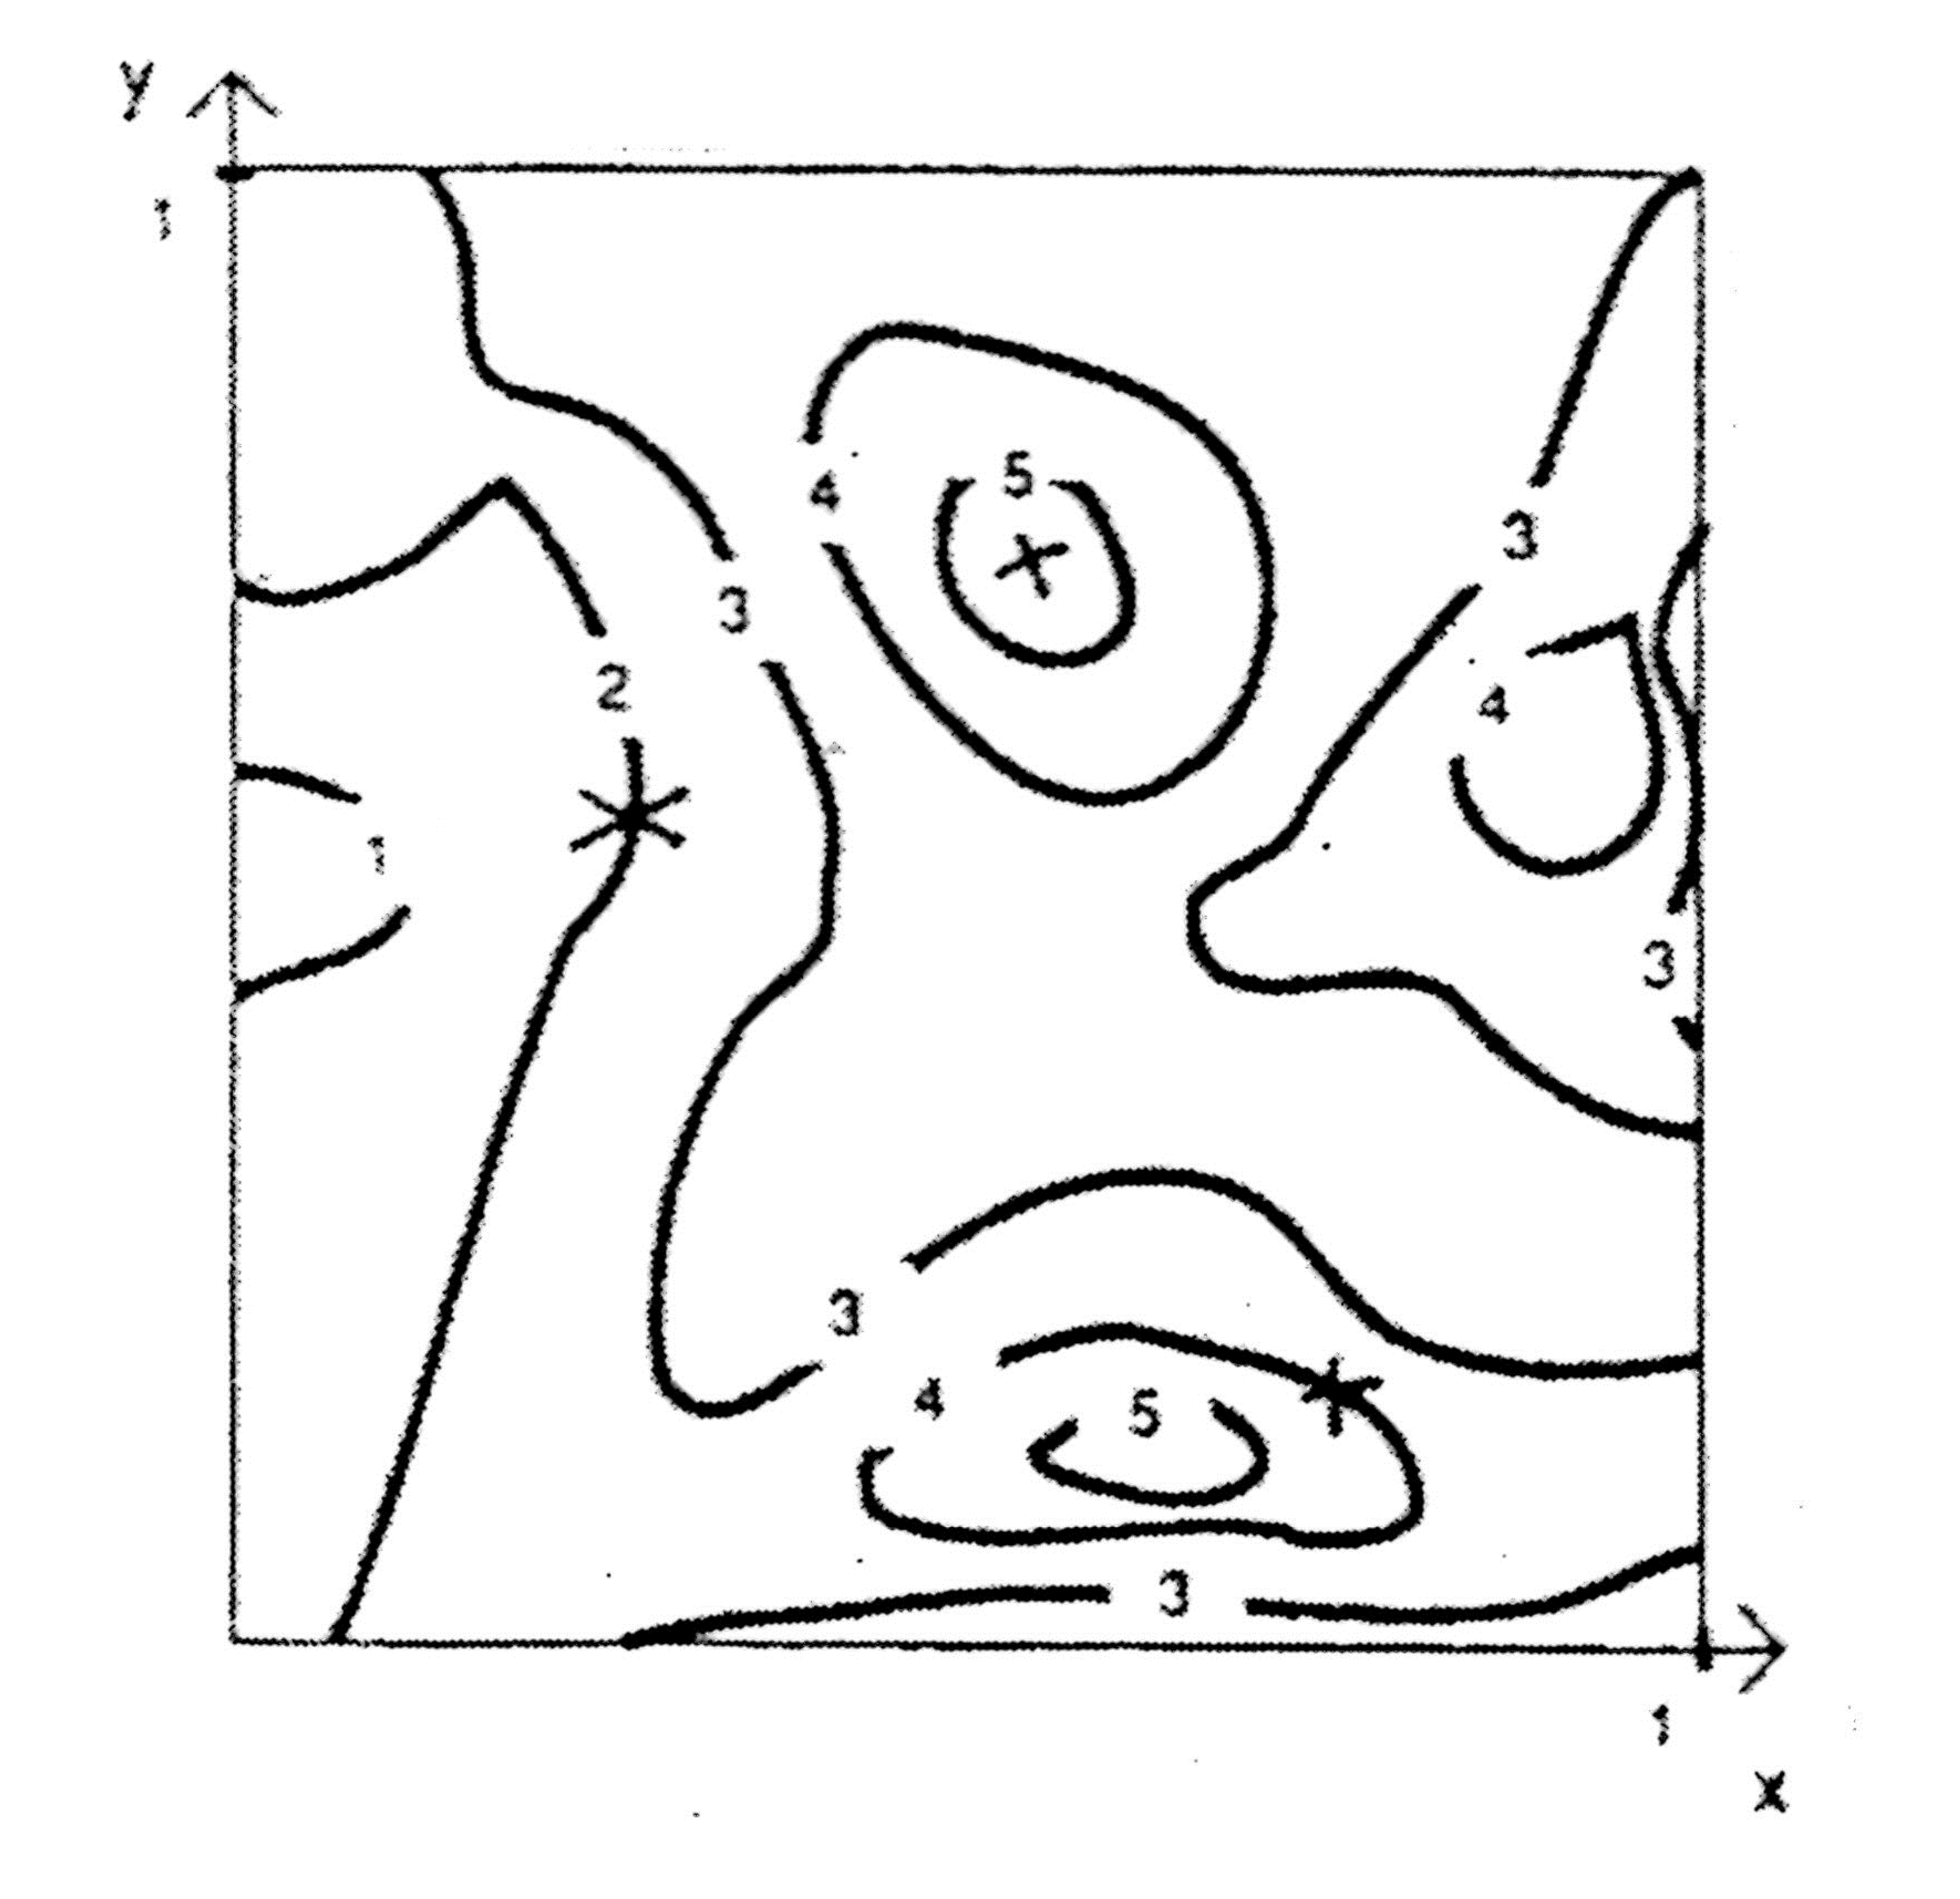
\includegraphics[scale=0.2]{Fig_291_1test.eps}
\end{center}
\end{exo}

%%EXE VI(Fonctions de plusieurs variables).16
\begin{exo}
Soit la fonction $f$ appliquant $(x,y)$ sur
$\displaystyle{\sqrt{\frac{x^2}{4}+\frac{y^2}{9}}}$. Après avoir
déterminé le domaine de $f$ et la nature du graphe de $f$,
faites un schéma dans un système d'axes $oxyz$

- du graphe de $f$;

- de quelques lignes de niveau de $f$ dans le plan $oxy$;

- des lignes correspondantes sur le graphe de $f$;

- de quelques gradients de $f$.
\end{exo}
\begin{exo}\ChoisirPourSeance{2014-2015}{geol=23,geog=23,irbi=23,chim=23,scie=23,biol=23,info=23}
Donner l'équation du plan tangent au graphe de la fonction
\begin{equation*}
f: {\BB R}^2\rightarrow\BB R :
(x,y)\mapsto(3+\ch(x+y))(1-5x+x^2)
\end{equation*}
au point $(0,0,0)$.
\end{exo}
\begin{exo}
Montrez que les plans tangents à la surface de ${\BB
R}^3$ d'équation
\begin{equation*}
z^2=(x-2)^2+(y+5)^2
\end{equation*}
passent tous par un même point~: donnez une preuve analytique et
une preuve géométrique (cette dernière considérera la
nature de la surface).
\end{exo}

%%EXE VI(Fonctions de plusieurs variables).18
\begin{exo}\ChoisirPourSeance{2014-2015}{geol=23,geog=23,irbi=23,chim=23,scie=23,biol=23,info=23}
Au point indiqué, dans quelle direction orientée la
fonction augmente-t-elle le plus~?

a) $\displaystyle{f:\BB
R^2:(x,y)\mapsto\cos(x \cdot y)\mbox{ au point
}(\sqrt\pi,\sqrt\pi);}$

b) $\displaystyle{f:\BB
R^3:(x,y,z)\mapsto 3x-2y+5z\mbox{ au point
}(6,7,8);}$

c) $\displaystyle{f:\BB
R^3:(x,y,z)\mapsto 4x^2-y^2+3z^2\mbox{ au point
}(1,-2,5);}$
\end{exo}
\begin{exo}
Déterminer l'erreur commise dans le raisonnement suivant. Soit $f(x,y) =
(x+y)^2.$ Posons $x=u-v$ et $y=u+v$. Alors
$$
\frac{\partial x}{\partial v}= -1, \qquad \frac{\partial y}{\partial v}=1,
\qquad \frac{\partial f}{\partial x}=\frac{\partial f}{\partial y}=2(x+y),
$$
donc
$$
\frac{\partial f}{\partial v}=\frac{\partial f}{\partial x}\frac{\partial
x}{\partial v}+\frac{\partial f}{\partial y}\frac{\partial y}{\partial v}=
-2(x+y) +2(x+y) = 0. \eqno(*)
$$
D'autre part, par la définition de $f$, il vient $f(u,v)=(u+v)^2$ et donc 
$$
\frac{\partial f}{\partial v}= 2(u+v) = 2y. \eqno(**)
$$
La comparaison de ($\star$) et ($\star\star$) prouve que la variable $y$ est toujours nulle.
\end{exo}
\begin{exo}
Pour le champ $\overrightarrow v$ de vecteurs sur $\BB R^2$
défini par
$$
\overrightarrow v(x,y)=\cos(x-y^2)\overrightarrow{e_x}+e^{xy}
\overrightarrow{e_y},
$$
calculer

a)
$(\overrightarrow{{\mathstrut\mbox{rot}}}\,\overrightarrow{\mathstrut
v})(\frac{\pi}{2},0)$;\qquad c)
$(\overrightarrow{\mathstrut\nabla}\times\overrightarrow {\mathstrut
v})(1,0)$;

b)  $(\mbox{div}\,\overrightarrow
{\mathstrut v})(0,0)$;\qquad d)
$(\overrightarrow{\mathstrut\nabla}\cdot\overrightarrow{\mathstrut
v})(0,-1)$.
\end{exo}

%%EXE VIII(Analyse vectorielle).1
\begin{exo}
Dans $\BB R^2$, calculer l'intégrale curviligne

a) $\displaystyle{\int_{C^+}x\,dy+y\,dx}$, \quad où $C^+$ est l'arc
de cubique défini par $y=x^3+x^2+x+1$ et $0\leq x\leq 1$;

b) $\displaystyle{\int_{C^+}\left((x^2-2xy)\overrightarrow{e_x}+(2xy+y^2)
\overrightarrow{e_y}\right)\cdot\overrightarrow{ds}}$, \quad où $C^+$
est l'arc de la parabole d'équation $y=x^2$, joignant le point
$(1,1)$ au point $(2,4)$;

c) $\displaystyle{\int_{C^+}(2a-y)\,dx+x\,dy}$, \quad où $a$ est
une constante réelle strictement positive et $C^+$ est l'arc de
cycloïde de paramétrisation
\begin{equation*}
\left\{
\begin{array}{l}
x=a(t-\sin t)\\[2mm]
y=a(1-\cos t)
\end{array}
\right.
\qquad 0\leq t\leq 2\pi;
\end{equation*}

d) $\displaystyle{\int_{C^+}(x^2+y)\,dx+(2x+y^2)\,dy}$, \quad où
$C^+$ est le carré de sommets $(1,1)$, $(1,2)$, $(2,2)$, $(2,1)$
parcouru une fois dans le sens anti-trignonométrique. Quel serait
le résultat si ce même carré était parcouru deux fois dans
le sens trigonométrique~?
\end{exo}
\begin{exo}
Calculer le travail de la force $\overrightarrow F$ lorsque le
cercle de $\BB R^2$ centré à l'origine et de rayon $R$ est
parcouru une fois dans le sens trigonométrique, si

a) $\overrightarrow
F(x,y)=(x+y)\overrightarrow{e_x}+(x-y)\overrightarrow{e_y}$;

b) $\overrightarrow
F(x,y)=xy\overrightarrow{e_x}+(x+y)\overrightarrow{e_y}$;

c) $\overrightarrow
F(x,y)=1.000.000\,\overrightarrow{e_x}-0,000.000.1\,
\overrightarrow{e_y}$.
\end{exo}

%%EXE VIII(Analyse vectorielle).2
\begin{exo}
Dans le plan $\BB R^2$, soit $T$ le triangle de sommets
$(0,0)$, $(1,0)$ et $(0,1)$, et $C^+$ son bord orienté dans le
sens trigonométrique. Soit le champ de vecteurs  $\overrightarrow
v$ sur $\BB R^2$, défini par
\begin{equation*}
 \overrightarrow v(x,y)=xy\,\overrightarrow{e_x}-x\,
\overrightarrow{e_y}.
\end{equation*}
Calculer l'intégrale circulaire $\displaystyle{\oint_{C^+}
 \overrightarrow{\mathstrut
v}\cdot\overrightarrow{\mathstrut{ds}}}$.
\end{exo}

%%EXE VIII(Analyse vectorielle).3
\begin{exo}
Soit $D$ le disque de rayon 3 centré à l'origine de $\BB
R^2$ et $C^+$ son bord orienté dans le sens trigonométrique.
Soit le champ de vecteur $\overrightarrow
v$ sur $\BB R^2$, défini par
\begin{equation*}
 \overrightarrow v(x,y)=x^2y\,\overrightarrow{e_x}-e^y\,
\overrightarrow{e_y}.
\end{equation*}
Calculer l'intégrale circulaire $\displaystyle{\oint_{C^+}
 \overrightarrow{\mathstrut
v}\cdot\overrightarrow{\mathstrut{ds}}}$.
\end{exo}
\begin{exo}
Calculer le champ de gradients de la fonction $f:\BB R^2\rightarrow \BB R:(x,y)\mapsto
x-y^2$. Dessiner les lignes de niveau $-1, 0, 1$ et 2 de $f$, ainsi
que les gradients de $f$ en quelques points, par exemple $(1,1)$,
$(0,1)$, $(1,0)$, $(3,1)$, $(3,-1)$. Donner de manière très
simple la valeur de l'intégrale curviligne
$\displaystyle{\int_{C^+}(\overrightarrow{\mbox{grad }}f)
\cdot\overrightarrow{ds}}$
si $C^+$ est la courbe orientée de paramétrisation
\begin{equation*}
\gamma:[0,\frac{\pi}{2}]\rightarrow\BB R^2:t\mapsto(\sin t,-\cos t).
\end{equation*} 
Même question si le domaine de
$\gamma$ est plutôt $[0,\pi]$.
\end{exo}
\begin{exo}
Considérons le champ de vecteurs $\overrightarrow v$ sur $\BB
R^2$ donné par
\begin{equation*}
\left\{
\begin{array}{lll}
v^x(x,y)&=&x-y\\[2mm]
v^y(x,y)&=&x+y
\end{array}
\right.
\end{equation*}
Calculer l'intégrale curviligne de $\overrightarrow v$ le long
des trois courbes orientées de $\BB R^2$ définies par les
paramétrisations
\begin{equation*}
\begin{array}{l}
\gamma_1:[0,1]\rightarrow\BB R^2:t\mapsto(t,t^2),\\[2mm]
\gamma_2:[1,0]\rightarrow\BB R^2:u\mapsto(1-u,(1-u)^2),\\[2mm]
\gamma_3:[1,2]\rightarrow\BB R^2:v\mapsto(\sqrt{v-1},v-1).
\end{array}
\end{equation*}
%Expliquez les ressemblances entre les valeurs trouvées.
\end{exo}

%%EXE VIII(Analyse vectorielle).4 (ici incomplet : manque "ramener à int double")
\begin{exo}
Dans $\BB R^2$, calculer l'intégrale circulaire 

a) $\displaystyle{\oint_{C^+}2(x^2+y^2)\,dx+(x+y)^2\,dy}$, \quad où
$C^+$ est le parcours simple du triangle de sommets $a=(1,1)$,
$b=(2,2)$, $c=(1,0)$ dans ce sens;

b) $\displaystyle{\oint_{C^+}xy^2\,dx-x^2y\,dy}$, \quad où
$C^+$ est la circonférence d'équation $x^2+y^2=16$ parcourue
trois fois dans le sens trigonométrique;

c) $\displaystyle{\oint_{C^+}\overrightarrow
F\cdot\overrightarrow{ds}}$, \quad où $\overrightarrow
F(x,y)=(x+y,y-x)$ et $C^+$ est obtenu en suivant du point $a=(1,0)$
au point $b=(2,3)$ une parabole d'axe $oy$, puis la droite de $b$
à $a$;

d)  $\displaystyle{\oint_{C^+}dx+x\,dy}$ \quad où $C^+$ est la
courbe refermée fabriquée à partir des paraboles
d'équations respectives $y=x^2$ et $x=y^2$;

e) $\displaystyle{\oint_{C^+}\overrightarrow
F\cdot\overrightarrow{ds}}$, \quad où $\overrightarrow
F(x,y)=x^3\,\overrightarrow{e_x}-y^3\,\overrightarrow{e_y}$ et
$C^+$ est la circonférence d'équation $x^2+y^2=1$ parcourue 5
fois dans le sens trigonométrique.
\end{exo}
\begin{exo}
Dans $\BB R^2$, calculer à l'aide d'une intégrale
circulaire l'aire de la région délimitée par

a) l'ellipse d'équations paramétriques
$$
\left\{
\begin{array}{c}
x=a\cos\theta\\
y=b\sin\theta
\end{array}
\right.
$$

b) la courbe d'équation $x^{2/5}+y^{2/5}=1$.
\end{exo}

%%EXE VIII(Analyse vectorielle).5
\begin{exo}
Dans $\BB R^2$, montrer que la valeur $I$ de l'intégrale
curviligne\\
$\displaystyle{\int_{C^+}(6x+2y)\,dx+(6y+2x)\,dy}$ est
indépendante de la courbe orientée joignant le point $(0,0)$ au
point $(1,1)$. Trouver deux fois cette valeur $I$ en prenant
d'abord $C^+$ rectiligne, puis $C^+$ situé sur la parabole
d'équation $y=x^2$. Déterminer une fonction $f:\BB
R^2\rightarrow\BB R$ dont le gradient au point $(x,y)$ est le
vecteur de composantes $(6x+2y, 6y+2x)$. Combien existe-t-il de
telles fonctions $f$~? Expliquer comment elles permettent toutes
d'obtenir très simplement la valeur $I$.
\end{exo}

%%EXE VIII(Analyse vectorielle).6
\begin{exo}
L'intégrale curviligne suivante est-elle dépendante de la
courbe orientée $C^+$ choisie pour se rendre dans $\BB R^2$ d'un
point $p$ à un point $q$~? Dans l'affirmative, déterminez deux
points $p$ et $q$ et deux courbes orientées joignant $p$ à $q$
sur lesquelles l'intégrale diffère. Dans la négative, trouvez
un champ scalaire $f$ sur $\BB R^2$ tel que la valeur de
l'intégrale soit $f(p)-f(q)$.

\begin{tabular}{ll}
a) $\displaystyle{\int_{C^+}(x^2\,\overrightarrow{e_x}
+y^2\,\overrightarrow{e_y})
\cdot\overrightarrow{ds}}$;\qquad\qquad\qquad&
c) $\displaystyle{\int_{C^+}y\cos dx+\sin x\,dy}$;\\[2mm]
b) $\displaystyle{\int_{C^+}(y^2\,\overrightarrow{e_x}
+x\,\overrightarrow{e_y})
\cdot\overrightarrow{ds}}$;&
d) $\displaystyle{\int_{C^+}e^y\,dx+e^x\,dy}$.
\end{tabular}
\end{exo}
\begin{exo}
Soit $C^+$ une courbe orientée lisse refermée de $\BB
R^2$, sans point multiple. Supposons que $C^+$ constitue le bord
d'un sous-ensemble compact $D$ de $\BB R^2$ tel que la formule de
Green soit valable pour tout champ de vecteurs de classe $\CCC^2$ sur
un certain ouvert $U$ contenant $D$. Considérons deux fonctions
$f$ et $g$ de classe $\CCC^2$ sur $U$.

a) Prouvez
$$
\displaystyle{
\dint{D}\left(\frac{\partial f}{\partial x}\,(x,y)+
\frac{\partial g}{\partial
y}\,(x,y)\right)\,dxdy=\int_{C^+}f(x,y)\,dy-g(x,y)\,dx
}.
$$

b) Déduisez du a) que l'aire de $D$ vaut à la fois
$$
\displaystyle{\int_{C^+}x\,dy}\qquad\mbox{et}\qquad
\displaystyle{\int_{C^+}y\,dx}.
$$

c) Notons $\overrightarrow n$ le vecteur normal unitaire à $C^+$,
orienté vers l'extérieur de $D$. Déduisez du a) la formule
suivante pour tout champ de vecteurs de classe $\CCC^2$ sur $U$~:
$$
\displaystyle{
\dint{D}\mbox{div }\overrightarrow
v\,dx\,dy=\oint_{C^+}\overrightarrow{\mathstrut
v}\cdot\overrightarrow{\mathstrut{ds}}}. $$
\end{exo}

%%EXE VIII(Analyse vectorielle).7
\begin{exo}
Soit $\overrightarrow v$ le champ de vecteurs sur $\BB R^2$
\begin{equation*}
\overrightarrow v(x,y)=3x^2y\,\overrightarrow{e_x}+(x^3+y^5)\,
\overrightarrow{e_y}.
\end{equation*}

a) Si $C^+$ est le carré de sommets $(2,0)$, $(0,2)$, $(-2,0)$,
$(0,-2)$ parcouru une fois dans le sens trigonométrique, que vaut
$\displaystyle{\oint_{C^+}
\overrightarrow{\mathstrut
v}\cdot\overrightarrow{\mathstrut{ds}}}$~?

b) Prouver que pour toute courbe refermée $C^+$ de $\BB R^2$
\begin{equation*}
\displaystyle{\oint_{C^+}
\overrightarrow{\mathstrut
v}\cdot\overrightarrow{\mathstrut{ds}}=0}.
\end{equation*}

c) Existe-t-il une fonction $f:\BB R^2\rightarrow \BB R$ telle que
\begin{equation*}
\left\{
\begin{array}{lll}
3x^2y&=&\displaystyle{\frac{\partial f}{\partial x}}\\[2mm]
x^3+y^5&=&\displaystyle{\frac{\partial f}{\partial y}}
\end{array}
\right.\quad?
\end{equation*}
\end{exo}
\chapter{Équations différentielles}\requires{chapter:Équations différentielles}

%%EXE XI(Equations différentielles du premier ordre).1
\begin{exo}\ChoisirPourSeance{2014-2015}{geol=24,geog=24,irbi=24,chim=24,scie=24,biol=24,info=24}
Pour quelle(s) valeur(s) réelle(s) de $a$ l'équation
différentielle en la fonction inconnue $\BB R\rightarrow\BB
R:t\mapsto y(t)$
\begin{equation*}
\displaystyle{\frac{dy}{dt}}(t)=(t-a)y(t)
\end{equation*}
admet-elle la solution
\begin{equation*}
\displaystyle{y(t)=C\,e^{r(t-1)^2}}
\end{equation*}
où $C$ et $r$ sont des constantes réelles données avec $C\neq
0$~?
\end{exo}

%%EXE XI(Equations différentielles du premier ordre).2
\begin{exo}
Trouver une équation différentielle du premier ordre
admettant pour solutions les fonctions $x\mapsto y=ax$, où $a$
est n'importe quel nombre réel.
\end{exo}

%%EXE XI(Equations différentielles du premier ordre).3
\begin{exo}
Trouver une équation différentielle du premier ordre admettant pour solutions au moins toutes les fonctions $y=y(x)$ satisfaisant
\begin{equation*}
x+a=e^xy
\end{equation*}
pour une certaine constante réelle $a$.
\end{exo}
\begin{exo}
D'après un météorologiste, la température $T$ dans
une certaine masse d'air est liée à l'altitude $h$~: le taux de
changement de $T$ par rapport à $h$ est proportionnel à $h$ et
au logarithme de $T$. Faut-il préciser en quelle base est pris le
logarithme~? Exprimer l'hypothèse du météorologiste par une
équation différentielle.
\end{exo}

%%EXE XI(Equations différentielles du premier ordre).4
\begin{exo}
Sans résoudre l'équation, déterminer le lieu des points
$(x,y)$ où la solution $y=y(x)$ de l'équation différentielle
$y'=xy-1$ atteint un minimum ou un maximum. Montrer que toutes les
solutions ont un graphe dans $\BB R^2$ qui coupe les axes sous un
angle constant.
\end{exo}
\begin{exo}
Dans quelle région du plan $\BB R^2$ les graphes des
fonctions solutions de l'équation différentielle
$y'=\sin(x^2+y^2)$ ont-ils une pente strictement positive~?
\end{exo}

%%EXE XI(Equations différentielles du premier ordre).5
\begin{exo}
Quelle équation différentielle caractérise la famille
des courbes d'équation $y=C_1x+C_2x^2$, où $C_1$ et $C_2$ varient
dans $\BB R$~?
\end{exo}
\begin{exo}
Soit l'équation différentielle $(x+y)dx+x\,dy=0$. Quel est
le lieu des points appartenant aux courbes représentant les
solutions $y$ de cette équation différentielle et en lesquels
$y'$ vaut 2~?
\end{exo}

%%EXE XI(Equations différentielles du premier ordre).6
\begin{exo}\ChoisirPourSeance{2014-2015}{geol=24,geog=24,irbi=24,chim=24,scie=24,biol=24,info=24,(a,,c,,d)}
Résoudre les équations différentielles du premier ordre
à variables séparables~:

a) $\displaystyle{y'\sqrt{1-x^2}}+xy=0$;

b) $(1-y^2)dy-y\,dx=0$;

c) $(1+y^2)x+(1+x^2)y'=0$;\\
pour les équations suivantes donner de plus la solution
particulière satisfaisant $y_0=y(x_0)$~:

d) $(x-4)xy'+y=0,\quad x_0=5,\quad y_0=-1$;

e) $(1+y)dx-(1+x)dy=0,\quad x_0=1,\quad y_0=2$.
\end{exo}

%%EXE XI(Equations différentielles du premier ordre).7
\begin{exo}
Quelle est la courbe de $\BB R^2$ qui représente une
solution de l'équation différentielle $y'=\ln^2x$ et qui coupe
la première bissectrice au point d'ordonnée égale à 1~?
\end{exo}
\begin{exo}
Montrer que la substitution $\displaystyle{y=\frac{t}{x}}$
réduit l'équation différentielle $y(1-xy)dx=x(1+xy)dy$ à
une équation à variables séparables. Résoudre l'équation
donnée.
\end{exo}
\begin{exo}
Une capacité se décharge au travers d'une résistance. Sa
charge $q$, fonction du temps $t$, satisfait
\begin{equation*}
\frac{dq}{dt}=i
\end{equation*}
où l'intensité $i$ du courant est donnée comme suit en
fonction du temps~:
\begin{equation*}
i=\displaystyle{-\frac{q_0}{RC}e^{-t/RC}.}
\end{equation*}
Dans cette expression, $q_0, R$ et $C$ sont des constantes ($q_0$
désigne la charge à l'instant initial $t=0$, $R$ la
résistance et $C$ la capacité).

a) Exprimer $q$ en fonction du temps et des constantes de
l'énoncé.

b) Les trois constantes $q_0, R$ et $C$ étant positives, la
charge augmente-t-elle~?

c) Pour $t$ tendant vers l'infini, la charge a-t-elle une valeur
limite~?
\end{exo}

%%EXE XI(Equations différentielles du premier ordre).8
\begin{exo}
Trouver la solution $y=y(x)$ de l'équation différentielle
\begin{equation*}
y'=(1+y^2)x^2
\end{equation*}
satisfaisant la condition initiale $y(0)=1$.
\end{exo}

%%EXE XI(Equations différentielles du premier ordre).9
\begin{exo}
Résoudre les équations différentielles du premier ordre
à fonction homogène:

a) $(x^3+y^3)-3xy^2y'=0$;

b) $(2x+3y)dx+(y-x)dy=0$;

c) $4y\,dx+x\,dy=0$;

d)
$\displaystyle{y\sqrt{x^2+y^2}\,dx-
x\left(x+\sqrt{x^2+y^2}\right)dy=0}$;

e) $\displaystyle{(x\sin\frac{y}{x}-y\cos\frac{y}{x})
+x\left(\cos\frac{y}{x}\right)\,y'=0}$.
\end{exo}
\begin{exo}
Résoudre les équations différentielles du premier ordre
en les ramenant à une équation à fonction homogène~:

a) $(3x+3y-4)y'+(x+y)=0$;

b) $(2x-5y-3)dx-(2x+4y-6)dy=0$;

c) $y'=(2x+3y+5)^2$;

d) $(3x+2y+1)dx-(3x+2y-1)dy=0$.
\end{exo}
\begin{exo}
Résoudre les équations de Bernoulli~:

a) $y'+2xy+xy^4=0$;

b) $xy'+y=x^3y^4$;

c) $y'-y=xy^2$;

d) $yy'-xy^2-x=0$;

e) $y'+y=y^2(\cos x-\sin x)$.
\end{exo}
\begin{exo}\ChoisirPourSeance{2014-2015}{geol=24,geog=24,irbi=24,chim=24,scie=24,biol=24,info=24}
Déterminer la solution générale de l'équation
différentielle
\begin{equation*}
\displaystyle{y'=-\frac{x+y}{x+6}},
\end{equation*}
ainsi que toutes les solutions particulières prenant la valeur 3
pour $x=2$.
\end{exo}

%%EXE XI(Equations différentielles du premier ordre).10
\begin{exo}\ChoisirPourSeance{2014-2015}{geol=24,geog=24,irbi=24,chim=24,scie=24,biol=24,info=24}
Résoudre les équations différentielles linéaires du
premier ordre~:

a) $y'+2xy=4x$;

b) $(x-2)y'=y+2(x-2)^3$;

c) $y'+y\cotg x=5e^{\cos x}$, et donner la solution particulière
par le point $\displaystyle{\left(\frac{\pi}{2},-4\right)}$;

d) $x\,dy-2y\,dx=(x-2)e^x\,dx$;

e) $\displaystyle{\frac{dr}{d\theta}+3r=2}$.
\end{exo}

%%EXE XI(Equations différentielles du premier ordre).11
\begin{exo}
Considérons l'équation différentielle
\begin{equation*}
(x^2+2x+5)y'-(x+1)y=x+1.
\end{equation*}

a) Déterminer la solution générale de cette équation
différentielle.

b) Combien de solutions particulières passent par le point
${(\frac{1}{2},\frac{3}{2})}$~? Déterminer toutes ces
solutions particulières.
\end{exo}

%%EXE XI(Equations différentielles du premier ordre).12
\begin{exo}
Résoudre les équations différentielles suivantes~:
lorsque des conditions initiales sont données, trouver les
solutions qui satisfont de plus ces conditions.\\[2mm]
\hfill\hspace*{6mm}
\begin{minipage}[t]{8cm}
a) $\displaystyle{(1+x^2)xy\,dy=(1+y^2)dx}$;\\[2mm]
b) $\displaystyle{y'-3\frac{y}{x}=\frac{x+1}{x}}$;\\[2mm]
c) $\displaystyle{y'-2\frac{y}{x+1}=(x+1)^3}$;\\[2mm]
d) $y'=0$;\\[2mm]
%e) $\displaystyle{3x^2y+8xy^2+(x^3+8x^2y+12y^2)y'=0}$;\\[2mm]
%f) $\displaystyle{(4x^3y^3-2xy)dx+(3x^4y^2-x^2)dy=0}$;\\[2mm]
e) $\displaystyle{y'=\frac{2x-1}{x^2}y+1}$;
%h) $\displaystyle{(y\ln x-1)y\,dx=x\,dy}$;\\[2mm]
\end{minipage}
\hfill
\begin{minipage}[t]{8cm}
f) $\displaystyle{y'+\frac{y}{2x}=\frac{1}{\sqrt x},\quad
x_0=4,\quad y_0=4}$;\\[2mm]
g) $\displaystyle{(1-x)dy-y^2dx=0}$;\\[2mm]
h) $\displaystyle{d\rho+\rho\tg\theta\,d\theta=0}$;\\[2mm]
i) $\displaystyle{x^3y'+(2-3x^2)y=x^3}$;\\[2mm]
%m) $\displaystyle{(x^2-2y^2)dy+2xy\,dx=0,}$\\[2mm]\phantom{m) }
%j) $x_0=1,\quad y_0=0$;\\[2mm]
j) $\displaystyle{ \sqrt{1-4x^2}\,dy+2\sqrt{1-y^2}\,dx=0}$.
%o) $\displaystyle{(3e^{3x}y-2x)dx+e^{3x}dy=0}$;\\[2mm]
%p) $\displaystyle{(x^2-2y^2)dy+2xy\,dx}$;\\[2mm]
%q) $\displaystyle{(6x^5y^3+4x^3y^5)}dx+$\\
%$\displaystyle{\qquad\qquad(3x^6y^2+5x^4y^4)dy=0}$.
\end{minipage} \hfill
\end{exo}

%%EXE XI(Equations différentielles du premier ordre).13
\begin{exo}
Résoudre l'équation différentielle
$y'+y\tg x=\sin 2x$, 
où $\displaystyle{-\frac{\pi}{2}<x<\frac{\pi}{2}}$.
\end{exo}

%%EXE XI(Equations différentielles du premier ordre).14
\begin{exo}
L'équation différentielle
\begin{equation*}
y'+yx=\displaystyle{\frac{x^3}{2y}}
\end{equation*}
admet-elle une solution passant par le point
$\displaystyle{(0,\frac{\sqrt 2}{2})}$~? Si oui, déterminer une
telle solution; est-elle unique~?
\end{exo}
\begin{exo}
Résoudre les équations différentielles suivantes, en
tenant compte des conditions initiales (CI) données~:

\hfill
\begin{minipage}[t]{6cm}
a) $\displaystyle{y'-xy=x^3}$;\\[2mm]
b) $\displaystyle{y'-\frac{a}{x}y=\frac{x+1}{x}}$\\
\hspace*{5mm}où $a\in\BB R\setminus\{0\}$);\\[2mm]
c) $\displaystyle{y'-\frac{2y}{x+1}=(x+1)^3}$;\\[2mm]
d) $\displaystyle{y'+\frac{1-2x}{x^2}y=1}$;\\[2mm]
e) $\displaystyle{y'\cos x+y\sin x=1}$;\\[2mm]
f) $\displaystyle{y'+y=e^{-x}}$;\\[2mm]
g) $\displaystyle{y'-y\tg x=\cos x}$;\\[2mm]
h) $\displaystyle{y'-\frac{2y}{x}=x^2e^x}$;\\[2mm]
i) $\displaystyle{}xy'+4y=x$;

\end{minipage}
\hfill
\begin{minipage}[t]{6cm}
j) $\displaystyle{y'(x+1)-2y=x+1}$\\[2mm]
\hspace*{5mm}(\mbox{CI : }$x_0=y_0=0)$;\\[2mm]
k) $\displaystyle{y'+\frac{y}{2x}=\frac{1}{\sqrt x}}$\\[2mm]
\hspace*{5mm}(\mbox{CI : }$x_0=y_0=4)$;\\[2mm]
l) $\displaystyle{x^3y'+(2-3x^2)y=x^3}$;\\[2mm]
m) $\displaystyle{y'+y\cotg x=5e^{\cos x}}$\\ 
\hspace*{5mm}(\mbox{CI : }$x_0=\frac{\pi}{2},\quad
y_0=-4)$;\\[2mm] 
n) $\displaystyle{y'+y\cos x=\frac{1}{2}\sin 2x}$\\
\hspace*{5mm}(\mbox{CI : }$x_0=y_0=2)$;\\[2mm]
%o) $\displaystyle{\frac{dy}{dx}+2xy+xy^4=0}$;\\[2mm]
%p) $\displaystyle{xy'+y=x^3y^4}$;\\[2mm]
%q) $\displaystyle{y'-y=xy^2}$;\\[2mm]
o) $\displaystyle{yy'-xy^2-x=0}$.
%s) $\displaystyle{y'+y=y^2(\cos x-\sin x)}$;\\[2mm]
%t) $\displaystyle{(y\ln x-1)y\,dx=x\,dy}$.
\end{minipage} \hfill
\end{exo}
\begin{exo}
Déterminer la solution générale et, lorsque des conditions
initiales sont données, la solution correspondante des
équations différentielles suivantes~:\\[2mm]
\hfill
\begin{minipage}[t]{8cm}
a) $\displaystyle{(x^2-yx^2)dy+(y^2+xy^2)dx=0},$\\[2mm]\phantom{a) }
$x_0=y_0=2$;\\[2mm] 
b) $\displaystyle{x\,dy-y\,dx=\sqrt{x^2+y^2}\,dx}$;\\[2mm] 
c) $\displaystyle{y-y'\cos x=y^2(1-\sin x)\cos x}$;\\[2mm] 
d) $\displaystyle{y'=\frac{7x+x+2}{3x+5y+6}}$;\\[2mm] 
e) $\displaystyle{y'+y\cotg x=\sin x}$;\\[2mm] 
f) $\displaystyle{y'+\frac{y}{x}-ay^2\ln x=0}$ (où $a\in\BB R^*$);\\[2mm]
g) $\displaystyle{y'+y\tg x=\seca^2x}$;\\[2mm] 
h) $\displaystyle{y'-y\seca x=1}$;\\[2mm] 
i) $\displaystyle{x(x^2+1)y'+(x^2-1)y=\frac{x^3}{1+x^2}}$;
\end{minipage} 
\hfill \begin{minipage}[t]{8cm}
j) $\displaystyle{y'-\frac{n}{x}y=e^xx^n,\quad\mbox{où }n\in\BB
N}$;\\[2mm]
k) $\displaystyle{x(1-x^2)dy+(2x^2-1)y\,dx=ax^3dx}$,\\
où $a\in\BB R\setminus\{0\}$;\\[2mm] 
l) $\displaystyle{y'+2y-4y^3=0}$;\\[2mm] m) $\displaystyle{\sin
y\,\frac{dy}{dx}=(1-x\cos y)\cos y}$;\\[2mm] 
n)
$\displaystyle{ye^{2x}dx-(1+e^{2x})dy=0}$;\\[2mm] 
o)
$\displaystyle{(x^2y-2xy^2)dx=(x^3-3x^2y)dy}$;\\[2mm] 
p)
$\displaystyle{(4x^2+3xy+y^2)dx+(4y^2+3xy+x^2)dy=0}$;\\[2mm] 
q)
$\displaystyle{\tg x\sin^2y\,dx+\cos^2x\cotg y\,dy=0}$;\\[2mm] 
r)
$\displaystyle{3e^x\tg y\,dx+(1-e^x)\seca^2y\,dy=0}$.
\end{minipage} \hfill
\end{exo}
\begin{exo}
Résoudre l'équation différentielle en la fonction
inconnue $t\mapsto y(t)$
\begin{equation*}
\frac{dy}{dt}(t)+y(t)=\max(\sin 3t,0).
\end{equation*}
\end{exo}

%%EXE XI(Equations différentielles du premier ordre).15
\begin{exo}
Soit l'équation différentielle
\begin{equation*}
\frac{dy}{dx}+y\,f(x)=\sin x.
\end{equation*}

a) Déterminer la fonction $f$ pour que cette équation admette
comme solution la fonction cosinus. Dans la suite, nous travaillons
avec cette fonction $f$.

b) Quelle est la solution générale de l'équation
différentielle~?

c) Quelle est la solution particulière qui admet un extrémum
pour $\displaystyle{x=\frac{\pi}{4}}$~?
\end{exo}
\begin{exo}
Quelle est la fonction solution de l'équation
différentielle $\displaystyle{(x^2+y^2)dx=2xy\,dy}$ et dont le
graphe coupe la droite d'équation $y=x+3$ au point d'abscisse
égale à $-2$~?
\end{exo}
\begin{exo}
Un certain mélange est formé d'un composant qui résiste
au temps, et d'un autre composant qui se volatilise à une vitesse
proportionnelle à la quantité de mélange présente à
l'instant considéré. Si $C_1$ est la quantité présente du
composant constant, $C_2$ celle du deuxième composant à
l'instant $t$ et $k$ le facteur de proportionnalité, exprimez
$C_2$ en fonction du temps $t$ et des constantes $C_1, C_2(0)$ et
$k$. Représenter graphiquement $C_2$ en fonction du temps.
\end{exo}
\begin{exo}
Lorsque deux certains produits chimiques $A$ et $B$ entrent en
réaction, une molécule de $A$ se lie à une molécule de $B$.
Notons $a$ le nombre de molécules de $A$ présente à l'instant
initial, et pareillement $b$ celui de $B$. Nous désignerons
encore par $y(t)$ le nombre de molécules du nouveau produit
formées après $t$ unités de temps.

a) Admettons que l'accroissement de $y$ par \og petit\fg{} intervalle de
temps soit proportionnel au nombre de molécules de $A$
présentes à ce moment, ainsi qu'au nombre de molécules de $B$
présentes à ce moment. Quelle équation différentielle en la
fonction inconnue $t\mapsto y(t)$ traduit cette hypothèse~?

b) Résolvez cette équation différentielle en supposant le
facteur de proportionnalité constant.

c) Si $a>b$, quelle est la valeur asymptotique de $y$ pour $t$
tendant vers $+\infty$~? Que signifie votre réponse en termes des
produits chimiques~?
\end{exo}
\begin{exo}
Désignons par $C(t)$ la quantité d'un certain médicament
présente dans le sang d'un patient à l'instant $t$. Ce
médicament est éliminé par l'organisme. Admettons que la
diminution de la quantité $C(t)$, sur l'intervalle de temps
$[t,t+h]$, c'est-à-dire $C(t+h)-C(t)$, soit approximativement
égale à $-k\,C(t)\,h$, où $k$ est une constante dépendant du
médicament.

Supposons d'abord qu'une seule injection soit faite au patient,
disons à l'instant $t=0$, d'une dose $C_0$ du médicament.

a) Le modèle considéré conduit à un problème de Cauchy
sur la fonction $C=C(t)$. Résolvez-le et faites un graphique de
$C$ en fonction du temps.

b) Montrez qu'à l'instant $\displaystyle{t=\frac{1}{k}}$, environ
63\% du médicament a été éliminé, et au temps 
$\displaystyle{t=\frac{2}{k}}$ environ 87\%.

Imaginons ensuite plutôt que le patient reçoive la même dose
qu'à l'instant 0 aux instants $T, 2T, 3T, \ldots$ Désignons par
$C_1$ la concentration du médicament immédiatement après la
deuxième injection, par $C_2$ cette concentration immédiatement
après la troisième injection \ldots

c) Calculer $C_1, C_2$ puis en général $C_{n-1}$.

d) Montrer que la suite $(C_n)$ est croissante et convergente.
Calculer $\displaystyle{\lim_{n\rightarrow\infty}C_n}$.

e) Représenter graphiquement la quantité $C(t)$ en fonction du
temps $t$.
\end{exo}
\begin{exo}
La transformation du trypsinogène en trypsine est
catalysée par la trypsine, et de ce fait la réaction s'emballe.
En notant $[A]$ la quantité de trypsinogène et $[B]$ la
quantité de trypsine au même instant, l'évolution de ces deux
quantités obéit à la loi
$$
-\frac{d[A]}{dt}=k[A][B],
$$
où $k$ est constante. Notons $A_0$ et $B_0$ les quantités
initiales; il faut aussi $[A]+[B]=A_0+B_0$ car toute la
trypsinogène se transforme en trypsine.

Établissez une expression donnant $[A]$ en fonction du temps.

Étudiez $[A]$ en fonction du temps.
\end{exo}
\begin{exo}
Considérons l'équation différentielle en la fonction
inconnue $U=U(t)$~:
$$
\displaystyle{\frac{d^3U}{dt^3}-3\frac{d^2U}{dt^2}+2\frac{dU}{dt}=0.}
$$

a) Combien de constantes d'intégration comporte la solution
générale de cette équation~?

b) Pour quelle(s) valeur(s) des constantes $\alpha$ et $\beta$ la
fonction $t\rightarrow \alpha t+\beta$ est-elle solution de
l'équation~?

c) Pour quelle(s) valeur(s) de la constante $\gamma$ la fonction
$\displaystyle{t\rightarrow e^{\gamma t}}$ est-elle solution de
l'équation~?

d) Quelle est la solution générale de l'équation~?

e) Cette équation admet-elle une solution qui soit une fonction
périodique~?
\end{exo}
\begin{exo}
Quelle est la solution générale de l'équation
différentielle
\begin{equation*}
pp
y''-6y'+9y=x+e^x ?
\end{equation*}
Déterminez toutes les solutions particulières $y$ telles que
$y(0)=2$.
\end{exo}
\begin{exo}
Déterminer toutes les fonctions $x\mapsto y(x)$ solutions de
l'équation différentielle
$$
y^{5/}-y^{3/}=0
$$
avec de plus $y^{2/}(0)=4$ et $y^{3/}(0)=1$.\\
Ces fonctions forment-elles un sous-espace vectoriel de ${\mathcal
C}^4(\BB R)$, l'espace de toutes les fonctions cinq fois
dérivables de $\BB R$ vers $\BB R$~? Ces mêmes fonctions
forment-elles un sous-espace affin de ${\mathcal
C}^4(\BB R)$~? Si oui, quelle est la dimension de ce sous-espace~?
\end{exo}
\begin{exo}
Résoudre les équations différentielles :

a) $y^{5/}-y^{2/}=0$;

b) $y^{2/}-y=\sin x$;

c) $y^{4/}-y^{2/}=x+\sin x$.
\end{exo}
\begin{exo}
Déterminer la solution générale de l'équation
différentielle

\hfill
\begin{minipage}[t]{6cm}
a) $y'''-4y''+3y'=x^2$;\\
b) $xy''-y'=x$;\\
c) $y'''-4y''=5$;
\end{minipage}
\hfill
\begin{minipage}[t]{8cm}
d) $y'''-y''+3y'-9y=0$;\\
e) $y'''-4y'=x$;\\
f) $y''''-3y''-4y=e^x$.
\end{minipage}
\hfill
\end{exo}

%%EXE XI(Equations différentielles du second ordre).1
\begin{exo}\ChoisirPourSeance{2014-2015}{geol=24,geog=24,irbi=24,chim=24,scie=24,biol=24,info=24}
Déterminer la solution générale des équations
différentielles suivantes~:

\hfill
\begin{minipage}[t]{6cm}
a) $y''-2y'=0$;\\
b) $y''-4y'+4y=0$;\\
c) $y''-4y'+3y=0$;\\
d) $2y''-y'=0$;\\
e) $y''-4y'=0$;\\
f) $y''+y'-12y=0$;\\
g) $y''+4y=0$;
\end{minipage}
\hfill
\begin{minipage}[t]{8cm}
h) $y''+y'+y=0$;\\
i) $y''+2y'+y=0$;\\
j) $y''-2y'-8y=0$;\\
k) $y''-7y'+10y=0$;\\
l) $y''+4y'+5y=0$;\\
m) $y''-4y'+13y=0$;\\
n) $y''-4y'+3y=0$.
\end{minipage}
\hfill
\end{exo}

%%EXE XI(Equations différentielles du second ordre).2
\begin{exo}
Déterminer la solution particulière des équations
différentielles suivantes répondant aux conditions initiales
indiquées~:

\begin{tabular}{lllll}
a) $y''+10y'+16y=0$,&\qquad &$x_0=0$,&\quad $y_0=1$,&\quad
$y'_0=12$;\\
 b) $y''-6y'+10y=0$,&\qquad  &$x_0=0$,&\quad
$y_0=1$,&\quad $y'_0=4$;\\
c) $y''+9y=0$,&\qquad   &$x_0=\frac{\pi}{3}$,&\quad
$y_0=1$,&\quad $y'_0=1$.
\end{tabular}
\end{exo}

%%EXE XI(Equations différentielles du second ordre).3
\begin{exo}\ChoisirPourSeance{2014-2015}{geol=24,geog=24,irbi=24,chim=24,scie=24,biol=24,info=24}
Déterminer la solution générale des équations
différentielles suivantes~:\\
\hfill
\begin{minipage}[t]{7cm}
a) $y''-6y'+13y=39$;\\
b) $y''+2y'+8y=4x^2-6x-3$;\\
c) $y''-2y'-3y=2x+1$;\\
d) $y''+9y=9e^{3x}$;\\
e) $y''-2y'+y=6e^x$;\\
f) $y''-5y'+6y=e^{-x}$;\\
g) $y''-y'-3y=e^{2x}$;\\
h) $y''-16y=2e^{-4x}$;\\
i) $y''-2y'+5y=10\sin x$;\\
j) $y''-5y'+6y=-3\sin x$;\\
k) $y''-5y'+4y=-2\cos x+8\sin x$;\\
l) $y''-2y'+2y=\cos 2x$;
\end{minipage}
\hfill
\begin{minipage}[t]{8cm}
m) $y''+y=\cos 2x$;\\
n) $y''+4y=\sin 2x-\cos 2x$;\\
o) $y''+y'=x^2$;\\
p) $y''-y=\sin x-\cos x$;\\
q) $y''+5y'+4y=3-2x$;\\
r) $y''+2y'+2y=x^2+\sin x$;\\
s) $y''-9y=x+e^{2x}-\sin 2x$;\\
t) $y''-3y'+2y=2x^2+1+e^x$;\\
u) $y''+2y'+4y=e^x\sin 2x$;\\
v) $y''+y=-2\sin x+4\cos x$;\\
w) $y''-2y'+y=\sin x+\sh x$;\\
x) $y''-6y'+9y=e^{3x}$.
\end{minipage}
\hfill
\end{exo}

%%EXE XI(Equations différentielles du second ordre).4
\begin{exo}\ChoisirPourSeance{2014-2015}{geol=24,geog=24,irbi=24,chim=24,scie=24,biol=24,info=24}
Déterminer la solution particulière des équations
différentielles suivantes répondant aux conditions initiales
indiquées~:

\begin{tabular}{llll}
a) $y''+3y'+2y=x^2+4x+8$,&\qquad $x_0=0$,&\quad $y_0=1$,&\quad
$y'_0=2$;\\ 
b) $y''-4y'+4y=e^{2x}+x^2$,&\qquad $x_0=0$,&\quad
$y_0=0$,&\quad $y'_0=0$;\\
c) $y''-2y'-3y=2x+1$,&\qquad $x_0=0$,&\quad
$y_0=\frac{1}{3}$,&\quad $y'_0=-\frac{4}{9}$;\\
d) $y''+4y=2\cos 2x$,&\qquad $x_0=0$,&\quad
$y_0=0$,&\quad $y'_0=\frac{1}{2}$.
\end{tabular}
\end{exo}

%%EXE XI(Equations différentielles du second ordre).5
\begin{exo}
Déterminer la courbe de $\BB R^2$
représentant la solution des équations différentielles
suivantes et répondant aux conditions imposées~:

\begin{tabular}{ll}
a) $y''-2y'+2y=2\sin x$,\qquad\qquad
&\begin{minipage}[t]{8cm}
courbe dont la tangente à l'origine est l'axe des abscisses;
\end{minipage}\\
b) $y''-2y'=2x$,\qquad
&\begin{minipage}[t]{8cm}
courbe dont la tangente au point $(0,2)$ est parallèle à l'axe
des abscisses; \end{minipage}\\
c) $y''-6y'+9y=x^2e^{3x}$,\qquad %% FIXME: n'est pas dans le formulaire.
&\begin{minipage}[t]{8cm}
$\alpha$) courbe dont la tangente au point $(0,1)$ a un coefficient
angulaire nul; \end{minipage}\\
&\begin{minipage}[t]{8cm}
$\beta$) courbe dont la tangente au point $(0,1)$ a une pente
égale à $-\frac{1}{4}$; \end{minipage}\\
d)\begin{tabular}[t]{l}1. $y''+4y=3\cos x$,\\
2. $y''+4y'=\sin 2x$,
\end{tabular}
&\begin{minipage}[t]{8cm}
courbe(s) passant par les points $(0,0)$ et
$\displaystyle{(\frac{\pi}{2},0)}$; \end{minipage}\\
e) $y''+4y=\sin 3x$,
&\begin{minipage}[t]{8cm}
courbe passant par les points $(0,2)$ et
$\displaystyle{(\frac{\pi}{4},\frac{9\sqrt 2}{10})}$. \end{minipage}
\end{tabular}
\end{exo}

%%EXE XI(Equations différentielles du second ordre).6
\begin{exo}
Sous quelles conditions sur les nombres réels $a, b, c$
l'équation différentielle $ay''+by'+cy=0$ n'admet-elle que des
solutions périodiques~?
\end{exo}

%%EXE XI(Equations différentielles du second ordre).7
\begin{exo}
Déterminer l'équation différentielle du second ordre
linéaire homogène à coefficients constants, dont la solution
générale est $y=Ce^{-x}\cos(2x+\varphi)$, où $C$ et $\varphi$
sont des constantes d'intégration.
\end{exo}
\begin{exo}
Montrer que les équations différentielles suivantes
admettent deux solutions particulières linéairement
indépendantes de la forme $x^\alpha$, avec $\alpha\in\BB R$~:

a) $x^2y''-2xy'+2y=0$;\hfill b) $x^2y''+4xy'+2y=0$;\hfill c)
$y''-\displaystyle{\frac{3y'}{x}}+\displaystyle{\frac{3y}{x^2}}=0$.

Résoudre ensuite les équations~:

a) $x^2y''-2xy'+2y=x^3\ln x$;\hfill b) $x^2y''+4xy'+2y=\ln x$;\hfill
c)
$y''-\displaystyle{\frac{3y'}{x}}+\displaystyle{\frac{3y}{x^2}}=2x-1$.
\end{exo}

%%EXE XI(Equations différentielles du second ordre).8
\begin{exo}\ChoisirPourSeance{2014-2015}{geol=24,geog=24,irbi=24,chim=24,scie=24,biol=24,info=24}
Soit l'équation différentielle $y''+2y'+my=12x^2e^{-x}$.

a) Déterminer la constante réelle $m$ de manière que
$y=x^4e^{-x}$ soit une solution particulière de cette équation.

b) Déterminer ensuite, pour cette valeur de $m$, la solution
générale.

c) Quelle est la solution particulière qui passe par les points
$(0,0)$ et $(1,1)$~?
\end{exo}

%%EXE XI(Equations différentielles du second ordre).9
\begin{exo}
Soit l'équation différentielle $y''-4y'+4y=f(x)$.

a) Déterminer $f(x)$ pour que $y=4x^2e^{2x}$ soit solution de
cette équation.

b) Déterminer ensuite la solution générale.

c) Déterminer la solution particulière dont le graphe est
tangent à la première bissectrice à l'origine des axes.
\end{exo}

%%EXE XI(Equations différentielles du second ordre).10
\begin{exo}
Déterminer les fonctions nulles à l'origine et telles que
leur dérivée première soit égale à l'opposé de la
dérivée seconde.
\end{exo}
\begin{exo}
Quelle est la courbe de $\BB R^2$ passant par l'origine et
admettant en chaque point une pente égale au triple de l'abscisse
du point~?
\end{exo}
\begin{exo}
Quelle est la courbe de $\BB R^2$ passant par le point
$\displaystyle{(\frac{1}{2},2)}$ dont la pente en chaque point est
proportionnelle au carré de l'ordonnée du point~?
\end{exo}
\begin{exo}
En tout point d'une courbe de $\BB R^2$, l'angle formé par la
tangente en ce point et l'axe des abscisses est complémentaire de
l'angle formé par la droite joignant le point à l'origine et
l'axe des abscisses. Caractériser cette courbe; est-elle unique~?
\end{exo}
\begin{exo}
La normale en un point quelconque d'une courbe de $\BB R^2$
passe toujours par un point fixe. Quelle est la nature de cette
courbe~?
\end{exo}
\begin{exo}
Un condensateur de capacité $C$ se décharge dans un circuit
comprenant une résistance $R$ et une self-induction $L$. La
charge $Q$, fonction du temps $t$, obéit à la loi
$$
\displaystyle{\frac{d^2Q}{dt^2}+\frac{R}{L}\frac{dQ}{dt}
+\frac{Q}{LC}=0.}
$$
Déterminer $Q$ en fonction de $t$ lorsque
$$
R=20\Omega\quad,\quad C=25\mu F\quad,\quad L=0{.}1F.
$$
Vers quel état évolue le circuit, et comment~?\\
Si, en outre, une différence de potentiel $V$ est appliquée aux
armatures du condensateur, l'équation à laquelle doit
satisfaire $Q$ est
$$
\displaystyle{L\frac{d^2Q}{dt^2}+R\frac{dQ}{dt}+\frac{Q}{C}=V}.
$$
Étudier le comportement du circuit lorsque $V$ est constant.
\end{exo}
\begin{exo}
Le mouvement d'une masse $M$ suspendue à un ressort de
coefficient d'élasticité $k$ est dans le vide déterminé par
l'équation
$$
\displaystyle{M\frac{d^2y}{dt^2}+ky=0}.$$
Déterminer ce mouvement et sa période s'il est périodique.\\
Si le mouvement a lieu dans un milieu tel que les forces de
frottement soient proportionnelles à la vitesse, l'équation
devient
$$
\displaystyle{M\frac{d^2y}{dt^2}+r\frac{dy}{dt}+ky=0}
$$
où $r$ est le coefficient de proportionnalité. Déterminer le
mouvement en prenant comme conditions initiales $t=0$, $y=A$,
$y'=0$ (discuter suivant les valeurs de $M, k$ et $r$).\\
Dans le cas d'un mouvement oscillatoire, déterminer la pseudo-période
et comparer avec la période du mouvement sans frottement.
\end{exo}
\begin{exo}
Le mouvement d'un pendule simple de longueur $l$ oscillant
d'un petit angle $\theta$ dans un milieu où la résistance est
proportionnelle à la vitesse est caractérisé par l'équation
$$
\displaystyle{\frac{d^2\theta}{dt^2}+2k\frac{d\theta}{dt}
+\frac{g}{l}\theta=0}.
$$
Déterminer le mouvement a) pour $k=0$\quad;\quad b) pour $k\neq
0$.\\
Discuter, dans ce dernier cas, en prenant comme conditions initiales
$\theta=\theta_0$ et $\displaystyle{\frac{d\theta}{dt}=0}$ en $t=0$.
\end{exo}
\begin{exo}\ChoisirPourSeance{2014-2015}{geol=24,geog=24,irbi=24,chim=24,scie=24,biol=24,info=24}
Étudier la solution générale de l'équation
différentielle du mouvement harmonique amorti
\begin{equation*}
\displaystyle{\frac{d^2x}{dt^2}+2k\frac{dx}{dt}+n^2=0}
\end{equation*}
dans les cas $n^2<k^2$, $n^2=k^2$, $n^2>k^2$.
Quand la solution représente-t-elle un mouvement oscillatoire~?
Lorsque $\displaystyle{\frac{k^2}{n^2}}$ est proche de zéro,
comparer la solution avec celle de l'oscillateur non amorti
(modification de la période, de l'amplitude).
\end{exo}
\begin{exo}
L'altitude $y$ d'une pierre, de masse $m$, lancée
verticalement (vers le haut) dans l'air, vérifie l'équation
différentielle $y''=-mg-\displaystyle{\frac{k}{m}}y'$ où $g$ et
$k$ sont des constantes strictement positives.

a) Calculez l'altitude de la pierre en fonction du temps, si sa
vitesse initiale est $v_0$ ($y'(0)=v_0$).

b) Déterminez la vitesse $v_0$ pour que l'altitude maximale de la
pierre soit $A$.
\end{exo}
\chapter{Intégrales multiples}\requires{chapter:Intégrales multiples}
\begin{exo}
Donner la valeur des intégrales suivantes~:
\begin{enumerate}
\item $\iint_D 3 \D x \D y$ où $D = \set{(x,y) \in \RR^2 \telque - 2 \leq x \leq 2, et -5 \leq y \leq 1}$;
\item $\iint_D -2 \D x \D y$, où $D = \intercc{0,3}\times\intercc{-2,-1}$ ;
\item $\iint_D \D x \D y$, où $D = \set{(x,y) \in \RR^2 \telque (x-4)^{2} + (y-3)^{2}\leq 9}$;
\item $\iint_D x  \D x \D y$, où $D = \intercc{-1,1}\times \intercc{0,3}$ ;
\item $\iint_D (x+y)  \D x \D y$, où $D = \set{(x,y) \in \RR^2 \telque x^{2}+y^{2} \leq 36}$.
\end{enumerate}
\end{exo}

\begin{exo}
\begin{enumerate}
\item $\iint_D (x+y)  \D x \D y$, où $D = \intercc{0,1}\times\intercc{0,1}$;
\item $\iint_D x \sin y  \D x \D y$, où $D = \intercc{0,1}\times \intercc{0,\pi}$;
\item $\iint_D (x+y)^{2}  \D x \D y$, où $D$ est la région bornée du plan délimitée par les trois droites d'équations respectives $x = 0$, $y = 0$, $x+y = 1$;
\item $\iint_D y^{2}  \D x \D y$, où $D$ est la couronne circulaire délimitée par les cercles de centre $(0,0)$ et de ayrons $1$ et $2$;
\item $\iint_D (x^{2}+y^{2}) \D x \D y$, où $D = \set{(x,y) \in  \RR^2\telque r_{1}^{2} \leq x^{2}+y^{2}\leq r_{2}^{2}}$ avec des constantes réelles $r_{1},r_{2}$ telles que $0 < r_{1} < r_{2}$;
\item $\iint_{D} y \D x \D y$, où $D = \set{(x,y) \in \RR^2 \telque x^{2} - y^{2} \leq 1 \text{ et } \abs{y} \leq 1}$;
\item $\iint_{D} x  \D x \D y$, où $D$ est le triangle plein de sommets $(0,0)$, $(1,1)$ et $(0,1)$.
\item $\iint_{D} \frac{1}{1+x^{2}+y^{2}}  \D x \D y$, où $D$ est la couronne circulaire délimitée par les cercles de centre $(0,0)$ et de rayons $1$ et $2$;
\item $\iint_{D} \frac{1}{x^{2}+y^{2}}  \D x \D y$, où $D$ est l'ensemble des $(x,y)$ vérifiant $r_{1}^{2}\leq x^{2}+y^{2} \leq r_{2}^{2}$, avec $r_{1}, r_{2}$ nombres réels tels que $0 < r_{1} < r_{2}$;
\item $\iint_{D} (x^2+y^{2})  \D x \D y$, où $D$ est défini par $x^{2}+y^{2} \leq 8x$;
\item $\iint_{D} \sqrt{1 - x^{2}-y^{2}}  \D x \D y$, où $D$ est défini par $xy < 0$ et $x^{2}+y^{2} \leq 1$.
\item $\iint_{D} \sqrt{1 - x^{2}-y^{2}}  \D x \D y$, où $D = \set{(x,y)\in \RR^2 \telque x \leq y \text{ et } x^{2}+y^{2} \leq y}$ ;
\item $\iint_{D} x^{2}y^{3}  \D x \D y$, où $D$ est le triangle plein de sommets $(0,3), (2,1)$ et $(3,5)$.
\end{enumerate}
\end{exo}

\begin{exo}
Si $f$ est une fonction continue de $D = \intercc{0,1}\times \intercc{0,1}$ vers $\RR$ à valeurs toutes positives ou nulles et $\iint_{D} f(x,y)  \D x \D y = 0$, faut-il que $f$ soit la fonction nulle sur $D$ ?
\end{exo}
\begin{exo}
Soit $S$ la surface de $\RR^3$ d'équation $z = 2 - x^{2} - y^{2}$. Faites un schéma de cette surface en dessinant aussi le système d'axes. Calculez ensuite le volume de la région située entre le plan d'équation $z = 0$ et la surface $S$, au dessus du plan $z = 0$. (Indice : utiliser une intégrable double en coordonnées polaires.)
\end{exo}
\begin{exo}
Calculer, à l'aide d'une intégrale double, l'aire (géométrique et non algébrique) de la région bornée de $\RR^2$
\begin{enumerate}
\item délimitée par les paraboles d'équations respectives $y^{2} = 10x + 25$ et $y^{2} = -6x + 9$ ;
\item délimitée par les courbes d'équations en coordonnées polaires $\rho = a (1+\cos \theta)$ et $\rho  = a \cos\theta$, où $a \in \RR^+_0$ ;
\item ne contenant pas l'origine et délimitée par les courbes d'équations $x^{2}+ y^{2} = 4$ et $x = 1$ respectivement;
\item délimitée par les droites d'équations $\theta = 0$ et $\theta = \frac{\pi}{4}$ en coordonnées polaires, ainsi que par l'arc de cercle de rayon $1$ centré à l'origine et intercepté par ces deux droites.
\end{enumerate}
\end{exo}

\begin{exo}
Calculer par intégrale double le volume de la région bornée de $\RR^3$ délimitée par les deux cylindres d'équations respectives $x^{2}+y^{2} = 1$ et $x^{2} + z^{2} = 1$.
\end{exo}

\begin{exo}
Déterminer
\begin{enumerate}
\item $\iiint_{D} (x+y+z) \D x \D y\D z$, si $D = \intercc{-1,1}\times\intercc{-1,1} \times\intercc{-1,1}$ ;
\item $\iiint_{D} 5 \D x \D y\D z$, si $D = \set{(x,y,z) \in \RR^{3} \telque (x-1)^{2} + (y-2)^{2} + (z-3)^{2} \leq 1}$ ;
\item $\iiint_{D}  \D x \D y \D z$, si $D = \set{(x,y,z) \in \RR^3 \telque 0 \leq x \leq 1, 0 \leq y \leq 1, 0 \leq z \leq 1 \text{ et } x^{2}+y^{2}+z^{2} \geq 1}$.
\end{enumerate}
\end{exo}
\begin{exo}
Calculer, par réduction à des intégrales simples,
\begin{enumerate}
\item $\iiint_{D} xyz  \D x \D y \D z$, où $D = \intercc{0,1}\times\intercc{0,1}\times\intercc{0,1}$;
\item $\iiint_{D}  y \D x \D y \D z$, où $D$ est la région bornée du premier octant de $\RR^3$ limitée par le plan d'équation $x + 2y + 3z = 1$.
\end{enumerate}
\end{exo}
\begin{exo}
Quelles sont les coordonnées cylindriques du point $(-1,1,2)$ de $\RR^3$ ?
\end{exo}
\begin{exo}
Quel est le point de $\RR^3$ dont les coordonnées sphériques sont $(10, \pi/2, \pi/4)$ ?
\end{exo}
\chapter{Complexes}\requires{chapter:Complexes}

%%EXE X(Nombres Complexes).1
\begin{exo}
Effectuer les opérations
\begin{equation*}
\begin{array}{llll}
\mbox{a) } &(1+i)+(3-2i)-4i; \qquad \qquad &\mbox{e) } &(1-i)^3; \\[2mm]
\mbox{b) } &(2-3i)(3-2i);    &\mbox{f) } &\displaystyle{\frac{1}{3-5i}}; \\[2mm]
\mbox{c) } &(3-i)(3+i); &\mbox{g) } &\displaystyle{\frac{2+i}{4-3i}}; \\[2mm]
\mbox{d) } &(3+2i)^2; &\mbox{h) } &\displaystyle{\frac{1-i}{i}}; \\[2mm]
&&\mbox{i) } &\left(\displaystyle{\frac{1-i}{1+i}}\right)^{10}.
\end{array}
\end{equation*}
\end{exo}

%%EXE X(Nombres Complexes).4
\begin{exo}
Calculer les racines carrées de~:
\begin{equation*}
\begin{array}{llll}
\mbox{a) } &i; \qquad \qquad &\mbox{c) } &-5-12i; \\
\mbox{b) } &50i; &\mbox{d) } &-21+20i. 
\end{array}
\end{equation*}
\end{exo}

%%EXE X(Nombres Complexes).2
\begin{exo}
Résoudre dans ${\BB C}$ les équations suivantes.
\begin{equation*}
\begin{array}{llrl}
\mbox{a) } &6x^2-12x+7=0;\qquad \qquad \qquad &\mbox{f) } &x^4-1=0; \\
\mbox{b) } &2x^4+x^2-1=0; &\mbox{g) } &x^3+x^2+x+1=0; \\
\mbox{c) } &x^2-x(4-i)+5+i=0; &\mbox{h) } &x^2-(2+3i)x+6i=0; \\
\mbox{d) } &x^2+x+3 \sqrt{2}i=0; &\mbox{j) } &x^3-1=0; \\
\mbox{e) } &x^2-(4 \pm 2i)x+12+4i=0; &\mbox{k) } &x^4-3x^2-4=0.
\end{array}
\end{equation*}
\end{exo}

%%EXE X(Nombres Complexes).3
\begin{exo}
On considère l'équation~:
\begin{equation*}
z^3-(1+8i)z^2-(15-8i)z+15=0.
\end{equation*}
\begin{enumerate}
\item Cette équation admet une racine réelle. Quelle est cette racine ? 
\item Rechercher toutes les racines de cette équation dans le champ 
des nombres complexes.
\end{enumerate}
\end{exo}

%%EXE X(Nombres Complexes).5
\begin{exo}
Calculer en se servant de la forme goniométrique\\
\indent~~~~1) $(3+3i)(-1+i \sqrt{3})$;\\ 
\indent~~~~2) $(-2-2i \sqrt{3})/(-1+i \sqrt{3})$; \\
\indent~~~~3) $(-1+i \sqrt{3})^{10}$; \\
\indent~~~~4) les racines carrées de $3-4i$; \\
\indent~~~~5) les racines cubiques de $1+i$;\\
\indent~~~~6) les racines cubiques de $2+2\sqrt{3}i$; \\
\indent~~~~7) les racines quatrièmes $1+i \sqrt{3}$; \\
\indent~~~~8) les racines sixièmes de $-27i$.
\end{exo}
\begin{exo}
Soit les ensembles $A, B$ et $C$ formés respectivement par les nombres complexes $z$ satisfaisant
\begin{equation*}
\vert z-2 \vert \leq 1, \qquad \vert z-i \vert \leq 2 \qquad \mbox{ et } 
\qquad \vert z-(2+2i) \vert \leq 2.
\end{equation*}
Représenter géométriquement ces ensembles dans le plan de Gauss.
\end{exo}
\begin{exo}
Démontrer que deux nombres complexes non réels sont conjugués ssi la somme et 
le produit de ces nombres sont réels.
\end{exo}

%%EXE X(Nombres Complexes).6
\begin{exo}
Soit $z=1-i \sqrt{3}$. 
\begin{enumerate}
\item Que vaut $z^5$ ?
\item Déterminer le plus petit nombre naturel strictement positif $n$ tel que $z^n$ 
soit réel.
\item Montrer qu'aucune puissance de $z$ n'est imaginaire pure.
\end{enumerate}
\end{exo}

%%EXE X(Nombres Complexes).7
\begin{exo}
Trouver toutes les solution complexes de l'équation
\begin{equation*}
z(z-2)^3=8z.
\end{equation*}
Représenter ces solutions dans le plan de Gauss et montrer que les points 
obtenus sont situés sur un cercle. Donner l'équation de ce cercle. 

\begin{correction}
  L'équation $z(z-2)^3=8z$ admet 0 comme solution évidente, puis on divise par 8 et on utilise la formule des racines de l'unité. Les solutions sont donc : $0$ et $2 + 2 \exp{\paren*{\frac{2k\pi}{3}}}$, c-à-d $0$, $4$ et $-1 \pm \sqrt 3 i$

  Pour le cercle, on remarque géométriquement que c'est celui de rayon $2$ centré en $2$. En effet, en prenant le module de l'équation on voit que si $z$ est non-nul, alors le module de $z-2$ vaut $2$. Or le module de $0-2$ vaut également $2$. Donc c'est vrai pour toutes les solutions.

  Les solutions sont $z = 0$ et $2 + 2 \exp{\paren*{\frac{2k\pi}{3}}}$ pour $k = 0,1,2$. C'est-à-dire
  \begin{equation*}
    0, 
  \end{equation*}
\end{correction}
\end{exo}

%%EXE X(Nombres Complexes).8
\begin{exo}
Trouver tous les nombres complexes $z$ tels que $z^2$ soit une 
racine carrée de $z$. 
\begin{correction}
  $z^2$ racine de $z$ ssi $z^4 = z$. De même, on a $z = 0$ et les racines cubiques
de $1$.
\end{correction}
\end{exo}

%%EXE X(Nombres Complexes).9
\begin{exo}
Où est l'erreur dans le raisonnement suivant ? Partons de 
$i=i$; donc $\sqrt{-1} = \sqrt{-1}$. Comme $-1= \displaystyle{\frac{1}{-1} = 
\frac{-1}{1}}$, on a $\displaystyle{\sqrt{\frac{-1}{1}} = \sqrt{\frac{1}{-1}}}$. 
Il en résulte que $\displaystyle{\frac{\sqrt{-1}}{\sqrt{1}} = 
\frac{\sqrt{1}}{\sqrt{-1}}}$ et $\displaystyle{\frac{i}{1} = \frac{1}{i}}$, 
d'où $i^2=1$.
\end{exo}

%%EXE X(Nombres Complexes).10
\begin{exo}
Combien existe-t-il de nombres complexes $z$ tels que $z^6=3$ ? 
Donnez les modules et les arguments de tous ces nombres.
\end{exo}

%%EXE X(Nombres Complexes).11
\begin{exo}
Comment se simplifie l'équation $x^3-3ix^2-3x-7i=0$ si l'on y remplace 
$x$ par $x+i$ ? En déduire les trois racines de l'équation initiale.
\end{exo}

\chapter{Analyse vectorielle}\requires{chapter:Analyse vectorielle}
%% Exos repris de MATH F 108
\begin{exo}
Dans $\RR^2$, calculer l'intégrale curviligne
\begin{enumerate}
\item $\int_{C} x \D y + y \D x$, où $C$ est l'arc de cubique paramétrée par $y = x^{3} + x^{2} + x + 1$ pour $0 \leq x \leq 1$;
\item $\int_{C} (x^{2} - 2xy, 2xy + y^{2}) \cdot \vec{\D s}$, où $C$ est l'arc de la parabole d'équation $ y = x^{2} $ joignant le point $(1,1)$ au point $(2,4)$;
\item $\int_{C} (2a - y) \D x + x \D y$, où $a$ est une constante réelle strictement positive et $C$ est l'arc de cycloïde de paramétrisation
  \begin{equation*}
    \begin{systeme}
      x & a (t-\sin t)\\
      y & a (1-\cos t)
    \end{systeme} \qquad 0 \leq t \leq 2\pi;
  \end{equation*}
\item $\int_{C} (x^{2} + y)\D x + (2x + y^{2})\D y$, où $C$ est le carré de sommets $(1,1), (1,2), (2,2), (2,1)$ parcouru une fois dans le sens anti-trigonométrique. Quel serait le résultat si ce même carré était parcouru deux fois dans le sens trigonométrique ?
\end{enumerate}
\end{exo}

\begin{exo}
Dans le plan $\RR^{2}$, soit $T$ le triangle de sommets $(0,0), (1,0)$ et $(0,1)$, et $C$ son bord orienté dans le sens trigonométrique. Soit le champ de vecteurs $\vec v$ défini sur $\RR^{2}$ par l'égalité
\begin{equation*}
  \vec v(x,y) = x y \vec{e_{x}} - x \vec{e_{y}}  
\end{equation*}
\begin{enumerate}
\item Calculer l'intégrale $\oint_{C} \vec v \cdot \vec{\D s}$ ;
\item Ramener cette intégrale à une intégrable double par application d'un théorème du cours, et calculer cette intégrale double directement.
\end{enumerate}
\end{exo}

\begin{exo}
Soit $D$ le disque de rayon $3$ centré à l'origine de $\RR^{2}$ et $C$ son bord orienté dans le sens trigonométrique. Soit le champ de vecteurs $\vec v$ défini sur $\RR^{2}$ par
\begin{equation*}
  \vec v(x,y) = x^{2} y \vec{e_{x}} - \exp{y} \vec{e_{y}}  
\end{equation*}
\begin{enumerate}
\item Calculer l'intégrale $\oint_{C} \vec v \cdot \vec{\D s}$ ;
\item Ramener cette intégrale à une intégrable double par application d'un théorème du cours, et calculer cette intégrale double directement.
\end{enumerate}
\end{exo}
\begin{exo}
Dans $\RR^2$, calculer les intégrales suivantes, soit directement, soit en se ramenant à une intégrale double.
\begin{enumerate}
\item $\oint_{C} 2(x^{2}+y^{2}) \D x + (x+y)^{2} \D y$ où $C$ est le parcours simple du triangle de sommets $(1,1), (2,2), (1,0)$ (dans cet ordre);
\item $\oint_{C} xy^{2} \D x - x^{2}y\D y$, où $C$ est la circonférence de rayon $4$ centrée en l'origine, parcourue trois fois dans le sens trigonométrique.
\item $\oint_{C} \vec F \cdot \vec{\D s}$, où $\vec F(x,y) = (x+y,y-x)$ et $C$ est obtenu en suivant d'abord, du point $(1,0)$ au point $(2,3)$, une parabole dont l'axe de symétrie est $oy$, puis le segment de droite qui retourne au point $(1,0)$ ;
\item $\oint_{C} \D x + x \D y$ où $C$ est la courbe fermée obtenue, partant de l'origine, en suivant $y = x^{2}$ puis $x = y^{2}$ ;
\item $\oint_{C} \vec F \cdot \vec {\D s}$ où $\vec F(x,y) = x^{3} \vec{e_{x}} - y^{3} \vec{e_{y}}$ et $C$ est la circonférence d'équation $x^{2}+y^{2} = 1$ parcourue cinq fois dans le sens trigonométrique.
\end{enumerate}
\end{exo}

\begin{exo}
Dans $\RR^{2}$, on considère
\begin{equation*}
I = \int_{C} (6x+2y)\D x + (6y +2x)\D y
\end{equation*}
où $C$ est une courbe joignant $(0,0)$ au point $(1,1)$.

\begin{enumerate}
\item Calculer $I$ pour $C$ le segment de droite joignant ces extrémités.
\item Calculer $I$ lorsque $C$ suit l'arc de parabole $y = x^{2}$.
\item Déterminer une fonction $f$ dont le gradient est $(6x+2y,6y+2x)$. Quelles sont toutes les telles fonctions ?
\item Utiliser l'une (quelconque) des fonctions du point précédent pour justifier l'égalité des résultats aux deux premiers points.
\end{enumerate}
\end{exo}

\begin{exo}
Dans chacune des intégrales suivante, prises chacune sur une courbe $C$ joignant des points $p$ et $q$, le résultat dépendra-t-il de la courbe elle-même ou seulement de ses extrémités $p$ et $q$ ? Prouver votre affirmation en trouvant soit un potentiel, soit deux chemins (de même extrémités) sur lesquels l'intégrale diffère.
\begin{enumerate}
\item $\int_{C} (x^{2} \vec{e_{x}} + y^{2} \vec{y_{y}})\cdot \vec{\D s}$;
\item $\int_{C} (y^{2} \vec{e_{x}} + x \vec{y_{y}})\cdot \vec{\D s}$;
\item $\int_{C} y \cos x \D x + \sin x \D y$;
\item $\int_{C} \exp{y} \D x + \exp{x}\D y$;
\end{enumerate}
\end{exo}

\begin{exo}
Soit $\vec v$ le champ de vecteurs sur $\RR^{2}$
\begin{equation*}
  \vec v(x,y) = 3 x^{2} y \vec{e_{x}} + (x^{3}+y^{5})\vec{e_{y}}.
\end{equation*}
\begin{enumerate}
\item Si $C$ est le carré de sommets $(2,0)$, $(0,2)$, $(-2,0)$, $(0,-2)$ parcouru une fois dans le sens trigonométrique, que vaut $\oint_{C} \vec v \cdot \vec{\D s}$ ?
\item Prouver que pour toute courbe fermée $C$ du plan,
  \begin{equation*}
    \oint_{C}\vec{v} \cdot \vec{\D s} = 0
  \end{equation*}
\item Existe-t-il une fonction $f : \RR^{2} \to \RR$ telle que
  \begin{equation*}
  \begin{systeme}
    3 x^{2}y & \pder f x\\
    x^{3} + y^{5} & \pder f y
  \end{systeme}~?
\end{equation*}
\end{enumerate}
\end{exo}

\begin{exo}
Soit $\gamma$ le chemin de $\RR^{3}$ d'équations
\begin{equation*}
  \begin{systeme}
    x & 8 y^{3}\\
    y & z^{3}
  \end{systeme}
\end{equation*}
limité aux points $(0,0,0)$ et $(8,1,1)$, et soit $\vec v$ le champ de vecteurs
\begin{equation*}
  \vec v (x,y,z) = x \unitvector x + y \unitvector y + z \unitvector z
\end{equation*}
\begin{enumerate}
\item Calculer l'intégrale curviligne
  \begin{equation*}
    \int_{\gamma} \vec v\cdot \vec {\D s}
  \end{equation*}
\item Vérifier que le rotationnel de $\vec v$ est nul.
\item Existe-t-il une fonction $F : \RR^{3} \to \RR$ dont le gradient est $\vec v$ ? Si oui, trouver une telle fonction.
\item Comment l'information trouvée au point précédent permet-elle de trouver rapidement la réponse au premier point ?
\end{enumerate}

\begin{correction}
  \begin{enumerate}
  \item Soit $\gamma(t) = (8 t^9, t^3, t)$ avec $t \in \intercc{0,1}$. On a $\gamma'(t) = (72 t^{8}, 3 t^{2}, 1)$, et donc
    \begin{equation*}
      \int_{\gamma} \vec v\cdot \vec {\D s} = \int_{0}^{1} 8 t^{9} 72 t^{8} + t^{3} 3 t^{2} + t \D t
    \end{equation*}
  \end{enumerate}
\end{correction}
\end{exo}

\begin{exo}
Dans $\RR^{3}$, calculer le flux au travers du morceau orienté $M$ de surface :
\begin{enumerate}
\item $\iint_M (x^2 \unitvector x + y \unitvector y + z \unitvector z) \cdot \vec n \D S$, où $M$ est la surface orientée donné par la paramétrisation~:
  \begin{equation*}
    [0,1]\times[0,1] \to \RR^{3} : (u,v) \mapsto (u,v,1-u-v)
  \end{equation*}
\item $\iint_{M} (6 z \unitvector x - 4 \unitvector y + 3 y \unitvector z) \cdot \D S$, où $M$ est la partie du plan d'équation $2x + 3y + 6z = 12$ située dans le premier octant ($x,y,z \geq 0$) et orientée vers le côté opposé à l'origine ;
\item $\iint_{M} (x^{2},xy,z^{2})\cdot \vec{\D S}$, où $M$ est la partie du plan d'équation $z = x$ situé au-dessus du carré de sommets $(1,0,0)$, $(1,1,0)$, $(0,1,0)$, $(0,0,0)$ et orientée vers le bas ;
\item $\iint_{M} (x^{2} \unitvector x + y^{2} \unitvector y)\cdot \vec  \D S$, où $M$ est la partie du plan d'équation $x + y + z = 1$ située dans le premier octant, orientée vers l'origine ;
\item $\iint_{M} (\unitvector x + \unitvector y + \unitvector z) \cdot \vec{\D S}$, où $M$ est le triangle de sommets $(-1,0,3)$, $(4,5,6)$ et $(1,1,1)$ orienté vers le haut.
\end{enumerate}
\end{exo}

\begin{exo}
Calculer dans $\RR^{3}$ le flux du champ de vecteurs donné par $\vec v (x,y,z) = (yz,xz,xy)$ au travers du triangle plein de sommets $(1,0,0)$, $(0,1,0)$, et $(0,0,1)$ orienté vers l'origine.
\end{exo}

\begin{exo}
Dans $\RR^{3}$ calculer le flux au travers de la surface orientée :
\begin{enumerate}
\item $\iint_{S} (x \unitvector x + y^{2} \unitvector y + z \unitvector z)\cdot \vec{\D S}$, où $S$ est la surface latérale de la \og boîte cylindrique\fg{} définie par $x^{2} + y^{2} = 4$ et $z \in \intercc{6,8}$;
\item $\iint_{S} (x,y,z)\cdot \vec n \D S$, où $S$ est la sphère unité centrée à l'origine, orientée vers l'intérieur;
\item $\iint_{S} (4xz \unitvector x + y^{2} \unitvector y + yz \unitvector z)\cdot \vec{\D S}$, où $S$ est la surface du tétraèdre délimité par les trois plans de référence et le plan d'équation $x + y + 2z - 2 = 0$, et $S$ est orienté vers l'origine.
\end{enumerate}
\end{exo}
\begin{exo}
Calculer dans $\RR^{3}$ le flux du champ de vecteurs $\vec v$ au travers de la surface orientée $S$ :
\begin{enumerate}
\item $\vec v (x,y,z) = (x,0,z)$ et $S$ a pour équation $z = x^{2}+ y^{2}$, restreinte à $z \leq 1$ et orientée vers le haut ;
\item $\vec v (x,y,z) = (xz^{2} + z) \unitvector x + (y x^{2} + x)\unitvector y + (zy^{2} + z)\unitvector z$ et $S$ est la sphère de rayon unité centrée en l'origine, orientée vers l'extérieur;
\item $\vec v(x,y,z) = x^{2} \unitvector x + y^{2} \unitvector y + z^{2} \unitvector z$ et $S$ est le carré de sommets $(1,0,0), (1,1,0), (1,1,1), (1,0,1)$ orienté par le vecteur normal $(-1,0,0)$.
\item $\vec v(x,y,z) = x \unitvector x + y \unitvector y + z^{2} \unitvector z$ et $S$ est le graphe de la fonction $[1,1] \times [2,2] \to \RR : (x,y) \mapsto x^{2}+y^{2}$.
\end{enumerate}
\end{exo}

\begin{exo}
Dans $\RR^{3}$, on considère l'intégrale circulaire
\begin{equation*}
  \int_{C} (z^{2}\unitvector + x^{2} \unitvector y + y^{2}\unitvector z)\cdot \vec{\D s},
\end{equation*}
où $C$ est la circonférence d'équations $x^{2} + y^{2} = 1$ et $z = 0$, parcourue une fois dans le sens trigonométrique (du demi-axe $ox^{+}$ vers le demi-axe $oy^{+}$).
\begin{enumerate}
\item Calculer cette intégrale.
\item Appliquer la formule de Stokes pour ramener cette intégrale curviligne à une intégrale de surface, en prenant comme surface le disque défini par le cercle $C$ (précisez l'orientation).
\item Calculer cette intégrale de surface.
\end{enumerate}
\end{exo}

\begin{exo}
On considère, dans $\RR^{3}$, le flux
\begin{equation*}
  \iint_{S} (\rot \vec w) \cdot \vec{\D S},
\end{equation*}
où $\vec w(x,y,z) = (x-z)\unitvector x + (x^{3} + yz) \unitvector y - 3xy^{2} \unitvector z$.
\begin{enumerate}
\item Calculer ce flux lorsque $S$ est la surface du cône d'équation $z = 2 - \sqrt{x^{2} + y^{2}}$ située au dessus du plan $oxy$, orientée vers $oz^{+}$ ;
\item Calculer le flux pour $S$ le disque défini par $z = 0$ et $x^{2} + y^{2} = 4$, orienté vers $oz^{-}$.
\item Expliquer le lien entre les deux valeurs trouvées.
\end{enumerate}
\end{exo}

\begin{exo}
Vérifier la formule d'Ostrogradsky pour le champ de vecteurs donné sur $\RR^{3}$ par $\vec v (x,y,z) = 4x \unitvector x - 2y^{2} \unitvector y + z^{2} \unitvector z$ et la région définie par $x^{2} + y^{2} \leq 4$ et $z \in \intercc{0,3}$.
\end{exo}
\begin{exo}
On considère, dans $\RR^{3}$, le flux
\begin{equation*}
  \iint_{S} (xy^{2} \unitvector x + yz^{2} \unitvector y + zx^{2} \unitvector z) \cdot \vec{\D S},
\end{equation*}
où $S$ est la sphère d'équation $x^{2} + y^{2} + z^{2} = 1$ orientée vers l'extérieur.
\begin{enumerate}
\item Calculer ce flux.
\item Ramener ce flux à une intégrale triple et calculer cette dernière.
\end{enumerate}
\end{exo}
\begin{exo}
Dans $\RR^{3}$, calculer directement puis en ramener à une intégrale triple :
\begin{enumerate}
\item $\iint_{S}  (x^{2} \unitvector x + y^{2} \unitvector y + z^{2} \unitvector z)$, où $S$ est la surface du cube $[0,9]^{3}\subset\RR^{3}$.
\item $\iint_{S} (x^{3} \unitvector x + y^{3} \unitvector y)\cdot \vec n \D S$, où $S$ est la sphère de rayon $1$ centrée à l'origine et orientée vers l'extérieur;
\item $\iint_{S} (x+y,y+z,z+x)\cdot \vec{\D S}$, où $S$ est la surface totale de la boîte cylindrique définie par
  \begin{equation*}
    \set{(x,y,z) \telque x^{2} + y^{2} \leq 1, z \in \intercc{0,1}}
  \end{equation*}
\item $\iint_{S} (y^{2},x^{2}, z^{2}) \cdot \vec  \D S$, où $S$ est le bord de la région définie par $x^{2} + y^{2} \leq z \leq 1$.
\end{enumerate}
\end{exo}
\chapter{Suites}\requires{chapter:Suites}
%%% Ceci n'a rien à voir ici :
\begin{exo}
Écrire les quatre premiers termes de chacune des suites suivantes~:
\begin{align*}
  a_{n} &= \frac{1}{3^{n}} & b_{n} &= \frac{n-1}{n+1} & c_{n} &= n - \frac{1}{n} \; (n > 0)
\end{align*}

\begin{correction}
Les valeurs sont reprises dans le tableau suivant.
% BEGIN RECEIVE ORGTBL valeur-de-qqes-suites
\begin{tabular}{lrlll}
n & 1 & 2 & 3 & 4\\
\hline
\((a_n)\) & 1/3 & 1/9 & 1/27 & 1/81\\
\((b_n)\) & 0 & 1/3 & 1/2 & 3/5\\
\((c_n)\) & 0 & 3/2 & 8/3 & 15/4\\
\end{tabular}
% END RECEIVE ORGTBL valeur-de-qqes-suites
% \begin{comment}
% #+ORGTBL: SEND valeur-de-qqes-suites orgtbl-to-latex
% | n       |   1 | 2   | 3    | 4    |
% |---------+-----+-----+------+------|
% | $(a_n)$ | 1/3 | 1/9 | 1/27 | 1/81 |
% | $(b_n)$ |   0 | 1/3 | 1/2  | 3/5  |
% | $(c_n)$ |   0 | 3/2 | 8/3  | 15/4 |
% \end{comment}
\end{correction}
\end{exo}
\begin{exo}
Pour chacune des propositions suivantes, compléter le blanc afin que l'implication soit vraie pour $\epsilon > 0$ et toute valeur entière de $n$.
\begin{enumerate}
\item $n > \ldots \Longrightarrow \frac{1}{2n} < \varepsilon$~;
\item $n > \ldots \Longrightarrow \frac{1}{3n^2} < \varepsilon$~;
\item $n > \ldots \Longrightarrow \abs{\frac{n}{1+n}-1} < \varepsilon$~;
\item $n > \ldots \Longrightarrow \abs{\frac{2n^2}{1+n^2}-2} < \varepsilon$.
\end{enumerate}

\begin{correction}
  Il suffit généralement de résoudre l'équation de droite afin de déterminer quelles valeurs de $n$ conviennent. 
  \begin{enumerate}
  \item Les solutions de l'inéquation sont $n < 0$ et $n > \frac{1}{2\varepsilon}$. La seconde inégalité est de la forme voulue, donc
    \begin{equation*}
      n > \frac{1}{2\varepsilon} \Longrightarrow \frac{1}{2n} < \varepsilon
    \end{equation*}
    convient. Cependant, toute valeur au delà de $\frac{1}{2\varepsilon}$ pourra être utilisée.
  \item Les solutions de l'inéquation sont $n < -\frac{1}{\sqrt{3\varepsilon}}$ et $n > \frac{1}{\sqrt{3\varepsilon}}$. Dès lors, la valeur $\frac{1}{\sqrt{3\varepsilon}}$ convient (ou toute valeur au delà de celle-là).
  \item L'inéquation se ré-écrit
    \begin{equation*}
      \abs{\frac{1}{1+n}} < \varepsilon
    \end{equation*}
    et ses solutions sont donc $n < - \frac{1}{\varepsilon} - 1$ et $n > \frac{1}{\varepsilon} - 1$. La valeur $\frac{1}{\varepsilon} - 1$ convient.
  \item L'inéquation se ré-écrit
    \begin{equation*}
      \abs{\frac{2}{1+n^{2}}} < \varepsilon
    \end{equation*}
    c'est-à-dire
    \begin{equation*}
      \frac{2}{1+n^{2}} < \varepsilon
    \end{equation*}
    ou encore
    \begin{equation*}
      n^{2} > \frac{2}{\varepsilon} - 1
    \end{equation*}
    et ses solutions sont donc, si $\varepsilon \leq 2$,
    \begin{equation*}
      n > \sqrt{\frac{2}{\varepsilon} - 1} \text{ et } n < - \sqrt{\frac{2}{\varepsilon} - 1}.
    \end{equation*}
    Lorsque $\varepsilon > 2$, toute valeur de $n$ fonctionne.

    Dès lors il suffit d'exiger $n > \sqrt{\frac{2}{\varepsilon} - 1}$ pour que l'implication soit satisfaite.
  \end{enumerate}
\end{correction}
\end{exo}
\begin{exo}
Parmi les suites suivantes, lesquelles sont croissantes ? décroissantes ? convergentes ? tendent vers $\infty$ ou $-\infty$ ? n'admettent pas de limite ?
\begin{multicols}{2}
  \begin{enumerate}
  \item $1, \frac 12, \frac 13, \ldots, \frac1n, \ldots$
  \item $1,2,3, \ldots, n, \ldots$
  \item $1,-1,1,\ldots,(-1)^{n}, \ldots$
  \item $u_{n} = \frac{n-1}{n+1}$
  \item $u_{n} = \frac 1 n \sin\paren*{\frac{\pi}{n}}$
  \item $u_{n} = \frac{\cos(n\pi)}{n}$
  \end{enumerate}
\end{multicols}

\begin{correction}
  % BEGIN RECEIVE ORGTBL comportement-de-suites
\begin{tabular}{lllllll}
                                             & Croiss.        & Décroiss.      & Cvgte          & \(+\infty\)    & \(-\infty\) & Pas de limite  \\
  \hline
  \(\sfrac1n\)                               &                & \(\checkmark\) & \(\checkmark\) &                &             &                \\
  \(n\)                                      & \(\checkmark\) &                &                & \(\checkmark\) &             &                \\
  \((-1)^{n}\)                               &                &                &                &                &             & \(\checkmark\) \\
  \(\sfrac{(n-1)}{(n+1)}\)                   & \(\checkmark\) &                & \(\checkmark\) &                &             &                \\
  \(\sfrac 1 n \sin\paren*{\sfrac{\pi}{n}}\) &                &                & \(\checkmark\) &                &             &                \\
  \(\sfrac{\cos(n\pi)}{n}\)                  &                &                & \(\checkmark\) &                &             &                \\
\end{tabular}
  % END RECEIVE ORGTBL comportement-de-suites
% \begin{comment}
%     #+ORGTBL: SEND comportement-de-suites orgtbl-to-latex
% |                                          | Croiss.    | Décroiss.  | Cvgte      | $+\infty$  | $-\infty$ | Pas de limite |
% |------------------------------------------+------------+------------+------------+------------+-----------+---------------|
% | $\sfrac1n$                               |            | \checkmark | \checkmark |            |           |               |
% | $n$                                      | \checkmark |            |            | \checkmark |           |               |
% | $(-1)^{n}$                               |            |            |            |            |           | \checkmark    |
% | $\sfrac{(n-1)}{(n+1)}$                   | \checkmark |            | \checkmark |            |           |               |
% | $\sfrac 1 n \sin\paren*{\sfrac{\pi}{n}}$ |            |            | \checkmark |            |           |               |
% | $\sfrac{\cos(n\pi)}{n}$                  |            |            | \checkmark |            |           |               |
% \end{comment}
\end{correction}
\end{exo}
\begin{exo}
Donner un exemple de suite
%\begin{multicols}{1}
  \begin{enumerate}
  \item convergente (dans $\RR$)~;
  \item ayant une limite infinie~;
  \item n'ayant pas de limite (ni finie, ni infinie)~;
  \item décroissante~;
  \item croissante et bornée~;
  \item bornée mais non-convergente.                   
  \end{enumerate}
%\end{multicols}
\begin{correction}
  Un exemple est donné dans chaque catégorie, parmi tant d'autres possibles !
  \begin{enumerate}
  \item convergente~: $u_{n} = \frac 1n$
  \item ayant une limite infinie~: $u_{n} = n$
  \item n'ayant pas de limite (ni finie, ni infinie)~: $u_{n} = (-1)^{n}$
  \item décroissante~: $u_{n} = \frac 1n$
  \item croissante et bornée~: $u_{n} = -\frac 1n$
  \item bornée mais non-convergente~: $u_{n} = (-1)^{n}$
  \end{enumerate}
\end{correction}
\end{exo}
\begin{exo}
Vérifier en utilisant la définition de la limite~:
\begin{multicols}{2}
  \begin{enumerate}
  \item $\limite n \infty \frac 1{2n} = 0$
  \item $\limite n \infty \frac n{1+n} = 1$
  \item $\limite n \infty \frac 1{2n+4} = 0$
  \item $\limite n \infty \frac 1{\sqrt{n}} = 0$
  \end{enumerate}\par\vfill
\end{multicols}
\begin{correction}
  \begin{enumerate}
  \item On veut vérifier~:
    \begin{equation*}
      \forall \epsilon > 0, \exists N : \forall n, n > N \Rightarrow \abs{\frac{1}{2n}} < \epsilon
    \end{equation*}
    Il faut donc trouver $N$. Ici, $N = \frac{1}{2\epsilon}$ convient.
  \item On veut vérifier
    \begin{equation*}
      \forall \epsilon > 0, \exists N : \forall n, n > N \Rightarrow \abs{\frac{n}{1+n} - 1} < \epsilon
    \end{equation*}
    Ici, $N = \frac{1}{\epsilon} - 1$ convient. On pourrait également prendre n'importe quelle valeur plus grande, par exemple $N = \frac{1}{\epsilon}$ serait bon.
  \item On veut vérifier~:
    \begin{equation*}
      \forall \epsilon > 0, \exists N : \forall n, n > N \Rightarrow \abs{\frac{1}{2n+4}} < \epsilon
    \end{equation*}
    Il faut donc trouver $N$. Ici, $N = \frac{1}{2\epsilon} - 4$ convient.
  \item On veut vérifier~:
    \begin{equation*}
      \forall \epsilon > 0, \exists N : \forall n, n > N \Rightarrow \abs{\frac1{\sqrt{n}}} < \epsilon
    \end{equation*}
    Ici $N = \frac{1}{\epsilon^{2}}$ convient.
  \end{enumerate}
\end{correction}
\end{exo}
\begin{exo}
Une suite réelle $(a_{n})$ vérifie la propriété suivante~:
\begin{equation*}
  \forall N \in \NN, \exists n > N : \abs{a_{n}} > \frac 14.
\end{equation*}
($n$ est un naturel). Donner si possible une suite convergente et une suite divergente vérifiant, chacune, cette propriété.

\begin{correction}
  Il suffit de prendre $a_{n}= 1$ (suite constante) et $a_{n} = (-1)^{n}$.
\end{correction}
\end{exo}
\begin{exo}
Si une suite réelle convergente vérifie $x_{n+1} = \frac 12 x_{n} + \frac 13 x_{n-1}$, quelle est la valeur de sa limite~?

\begin{correction}
  Si la suite converge, disons vers $a$, alors sa limite doit vérifier $a = \frac{1}{2} a + \frac{1}{3} a$, et donc $a = 0$ est la seule valeur possible.

  Notons que la relation donnée ne définit pas une suite unique: il faut encore spécifier $x_0$ et $x_{1}$. La question de savoir pour quelles valeurs de $x_{0}$ et de $x_{1}$ la suite converge effectivement n'est pas posée dans cet exercice. Néanmoins, pour information, la réponse est qu'une telle suite converge toujours.
% Le polynôme caractéristique de cette relation est $x^{2} - 1/2 x - 1/3$ dont les racines sont 1/4 \pm 1/2 sqrt(19/6), disons u et v.
% La suite s'écrit donc a_n = A u^n + B v^n où A+B = a_0 et A u + B v = a_1
% Comme u et v sont entre -1 et 1, une telle suite converge toujours vers 0.
\end{correction}
\end{exo}
\begin{exo}
On considère deux suites croissantes, $(x_n)$ et $(y_n)$. Démontrez ou infirmez à l'aide d'un contre-exemple,
\begin{enumerate}
\item la suite $(x_n+y_n)$ est croissante.
\item la suite $(x_ny_n)$ est croissante.
\end{enumerate}

\begin{correction}
  \begin{enumerate}
  \item vrai. Les hypothèses sont $x_{n+1} \geq x_{n}$  et  $y_{n+1} \geq y_{n}$ pour tout $n$. Or on peut additionner ces inégalités membre à membre, donc $x_{n+1} + y_{n+1} \geq x_{n} + y_{n}$ est vraie pour tout $n$ également. Ceci prouve la croissance de la somme.
  \item faux: prendre $x_k=-\frac{1}{k}$ et $y_k=k^3$. Le produit donne $-k^{2}$, ce qui n'est clairement pas croissant.
  \end{enumerate}
\end{correction}
\end{exo}
\begin{exo}
Montrer que la suite $(u_{n})$ définie par $u_{n} = 1 + \frac{\exp{-n}}{n}$ converge vers $1$.
\begin{correction}
  C'est une application des règles de caclul : $n \exp{n}$ tend vers l'infini, donc  $\frac{\exp{-n}}{n}$ tend vers $0$, et le résultat suit.
\end{correction}
\end{exo}
\begin{exo}
Montrer que la suite réelle $\log_{n}(10)$ (pour $n \geq 2$) tend vers $0$.
\begin{correction}
  Notons $x_{n} = \log_n(10)$. Soit $\epsilon > 0$. On veut montrer qu'il existe $N$ tel que que si $n > N$, on a $x_{n} < \epsilon$. C'est-à-dire nous voulons $10 < n^{\epsilon}$ (l'exponentielle $x \mapsto n^{x}$ étant croissante, l'inégalité est préservée), il suffit alors de prendre $n > 10^{\frac 1 \epsilon}$ (l'application $x \mapsto x^{\epsilon}$ étant croissante si $\epsilon > 0$, cette inégalité implique l'inégalité précédente).
\end{correction}
\end{exo}
\begin{exo}
Pour chaque affirmation, déterminer si elle est vraie (et démontrer en invoquant un théorème du cours) ou fausse (et démontrer par un contre-exemple). Les suites sont supposées être des suites de nombres réels.
\begin{enumerate}
\item Tout suite bornée est convergente.
\item Toute suite bornée admet une sous-suite convergente.
\item Toute suite bornée croissante admet une sous-suite convergente.
\item Toute suite non-convergente est non-bornée.
\end{enumerate}
\begin{correction}
\begin{enumerate}
\item Tout suite bornée est convergente : faux. Par exemple $(-1)^{n}$.
\item Toute suite bornée admet une sous-suite convergente : vrai (mais la preuve n'est pas complètement évidente)
\item Toute suite bornée croissante admet une sous-suite convergente : vrai (en fait toute suite bornée croissante est elle-même convergente).
\item Toute suite non-convergente est non-bornée : faux. Par exemple $(-1)^{n}$ est non-convergente mais n'est pas non-bornée.
\end{enumerate}
\end{correction}
\end{exo}
\begin{exo}
Le but est ici de démontrer que si $a$ est tel que $\abs a < 1$, alors $\limite n \infty a^{n} = 0$. 
\begin{enumerate}
\item Si $1 > a > 0$, montrer que $h \pardef \frac{1}{a} - 1$ est strictement positif.
\item Utiliser la formule du binôme de Newton pour démontrer l'inégalité
  \begin{equation*}
    (1+h)^{n} > nh
  \end{equation*}
  pour tout $h > 0$ et $n \in \NN$.
\item Grâce aux points précédents, montrer que pour tout $1 > a > 0$ nous avons~:
  \begin{equation*}
    a^{n} < \frac{1}{n \paren*{\frac{1}{a} - 1}}.
  \end{equation*}
\item Conclure que $a^{n}$ tend vers $0$ lorsque $a \in \interoo{0,1}$
\item Généraliser à $a$ quelconque (avec $\abs a < 1$).
\end{enumerate}
\begin{correction}
\begin{enumerate}
\item Comme $0 < a < 1$, on a (en multipliant par l'inverse de $a$) $\frac 1 a > 1$. En soustrayant $1$, on obtient $h \pardef \frac{1}{a} - 1 > 0$.
\item Si $h > 0$, le binôme de Newton nous apprend~:
  \begin{equation*}
    (1+h)^{n} = \sum_{j=0}^{n} \binom{n}{j} h^{j} 1^{n-j} = 1 + n h + \frac{n(n-1)}{2} h^{2} + \cdots
  \end{equation*}
  Or tous les termes de cette somme sont positifs. Donc le tout est plus grand qu'une partie :
  \begin{equation*}
    (1+h)^{n} > nh.
  \end{equation*}
\item En utilisant notamment le $h$ défini au premier point dans le second point, nous obtenons :
  \begin{equation*}
    {\paren*{\frac 1 a}}^{n}= (1+h)^{n} > nh = n \paren*{\frac{1}{a} - 1} > 0
  \end{equation*}
  ce qui prouve, en inversant :
  \begin{equation*}
    a^{n} < \frac{1}{n \paren*{\frac{1}{a} - 1}}.
  \end{equation*}
\item Le membre de droite de l'inéquation précédente tend vers $0$ lorsque $n$ tend vers l'infini. Dès lors $a^{n}$ (qui est positif) tend vers $0$ lorsque $a \in \interoo{0,1}$
\item Lorsque $a = 0$, la suite $a^{n}$ est constante égale à $0$, donc tend vers $0$. Lorsque $a$ est entre $-1$ et $0$ (strictement), alors $\abs a \in \interoo{0,1}$, donc $\abs {a^{n}} = \abs a^{n}$ tend vers $0$ par la discussion précédente. Ceci montre que $a^{n}$ tend vers $0$ également. Dès lors, $a^{n}$ tend vers $0$ dès que $\abs a < 1$.
\end{enumerate}
\end{correction}
\end{exo}
\begin{exo}
Le but est ici de démontrer que si $a > 0$, alors $\limite n \infty \sqrt[n]{a} = 1$.%% On suppose que l'exo a^n -> 0 a été montré.
\begin{enumerate}
\item Si $a > 1$, vérifier que $h_{n} \pardef \sqrt[n]{a} - 1$ est strictement positif et montrer l'inégalité $(1+h_{n})^{n} > n h_{n}$. En déduire le résultat (pour $a > 1$).
\item Si $0 < a < 1$, poser $b = \frac 1a$ et montrer le résultat.
\end{enumerate}
\begin{correction}
  \begin{enumerate}
  \item Si $a > 1$, alors $\sqrt[n]{a} > 1$ (puisque $x \mapsto \sqrt[n]{x}$ est croissante sur $\RR^{+}$), donc $h_{n} \pardef \sqrt[n]{a} - 1 > 0$. Or nous avons déjà montré que $(1+h_{n})^{n} > n h_{n}$ dans un exercice précédente. Nous en déduisons
    \begin{equation*}
      a > n h_{n} > 0 \text{ c'est-à-dire }  0 < h_{n} < \frac a n
    \end{equation*}
    Le membre de droite tend vers $0$, donc $h_{n}$ également.
  \item Si $0 < a < 1$, on pose $b = \frac 1a$. Comme $b > 1$, on a : $\sqrt[n]b$ tend vers $1$. Comme $\sqrt[n]a = \frac{1}{\sqrt[n]{b}}$, nous avons : $\sqrt[n]{a}$ tend vers $1$. Trivialement si $a = 1$, $\sqrt[n]{1}$ tend vers $1$ (suite constante). Dès lors ceci prouve que $\sqrt[n] a$ tend vers $1$ pour tout $a > 0$.
  \end{enumerate}
\end{correction}
\end{exo}
\begin{exo}
Démontrer $\limite n \infty \sqrt[n]{n} = 1$. Indication : poser $h_{n} \pardef \sqrt[n]{n} - 1$, puis montrer et utiliser l'inégalité
\begin{equation*}
  n > \frac 12 n (n-1) h_{n}^{2}
\end{equation*}
lorsque $n \geq 2$.

\begin{correction}
  En utilisant l'indication et l'astuce
  \begin{equation*}
    (h_{n} + 1)^{n} > 12 n (n-1) h_{n}^{2}
  \end{equation*}
  (le membre de droite est un terme du développement, via la formule de Newton, du membre de gauche), on obtient l'inégalité suggérée. On en déduit
  \begin{equation*}
    \frac{2}{n-1} > h_{n}^{2}
  \end{equation*}
  ce qui prouve
  \begin{equation*}
    \sqrt{\frac{2}{n-1}} > h_{n} > -\sqrt{\frac{2}{n-1}}
  \end{equation*}
  et donc $h_{n}$ tend vers $0$. Donc $\sqrt[n]n$ tend vers $1$.
\end{correction}
\end{exo}
\begin{exo}
  Soit une suite $(x_{n})$ vérifiant
  \begin{equation*}
    x_{n+1} = f(x_{n}) \qquad \text{où $f(x) \pardef \frac{1}{1+x} + 1$}
  \end{equation*}
  pour tout $n$. Notons qu'il suffit de fixer $x_{0}$ (à une valeur autre que $-1$) pour que la suite soit bien déterminée.
  \begin{enumerate}
  \item Tracer le graphe de $f$ ainsi que la première bisectrice ($y=x$) dans un même repère cartésien.
  \item En s'aidant des graphes ci-dessus, décrire géométriquement quelques valeurs de la suite si $x_{0} = 0$.
  \item Si $x_{0} = \sqrt{2}$, écrire quelques valeurs de cette suite (simplifier au maximum !)
  \item Démontrer l'égalité $\frac{-1}{1+\sqrt{2}} = 1 - \sqrt{2}$.
  \item Pour $x > 0$, démontrer :
    \begin{equation*}
      \abs{f(x) - \sqrt{2}} \leq k \abs{x - \sqrt 2}.
    \end{equation*}
    où $k < 1$ est une constante à spécifier.
  \item En déduire l'inégalité
    \begin{equation*}
      \abs{f^{n}(x) - \sqrt{2}} \leq k^{n} \abs{x-\sqrt 2}
      \qquad \text{où $f^{n}(x) \pardef f(f(\cdots f(x)))$}
    \end{equation*}
    pour tout $n \geq 1$ et tout $x > 0$.
  \item Conclure $x_{n} \to \sqrt 2$ si $x_{0} > 0$, puis généraliser pour $x_{0} > -1$. % (Indication: si $-1 < x_{0} < 0$, alors $x_{1} > 0$.)
  \item (difficile) Quelle est la limite si $x_{0} < -1$ ?
  \end{enumerate}
  \begin{correction}
    \begin{enumerate}
    \item
    \item
    \item C'est une suite constante.
    \item L'égalité se montre en la multipliant par le dénominateur.
    \item On a :
      \begin{align*}
        \abs{f(x) - \sqrt{2}} &= \abs{\frac1{1+x} + 1 - \sqrt{2}} && \\
                              &= \abs{\frac 1{1+x} - \frac 1{1+\sqrt{2}}} && \text{par le point d}\\
                              &= \abs{\frac{\sqrt{2} - x}{(1+x)(1+\sqrt{2})}} && \text{mise au même dénominateur}\\
                              &\leq \abs{\frac{\sqrt{2} - x}{1+\sqrt{2}}} && \text{car : $x > 0$ donc $\frac{1}{1+x} < 1$}\\
                              &= k \abs{x - \sqrt{2}} && \text{en posant $k = \frac1{1+\sqrt{2}}$}
      \end{align*}
    \item Par récurrence : c'est vrai pour $n = 1$ puisque c'est le point précédent. Ensuite il suffit de vérifier que $f^{n}(x) > 0$ pour tout $n$, et la récurrence suit facilement. (FIXME: à faire).
    \item $k^n$ tend vers $0$, donc le théorème du sandwich s'applique. Lorsque $x_{0} > -1$ mais $x_{0} < 0$, on note que $x_{1} > 0$, ce qui permet d'utiliser le même raisonnement que lorsque $x_{0} > 0$.
    \item (ce point est plus difficile). Je crois que la réponse est ceci, mais je n'ai pas fait les détails : soit $E$ l'ensemble contenants $-1$ et ses antécédents successifs : $-1, (f^-1)(-1), (f^-2)(-1), ...$.
      \begin{itemize}
      \item Si $x = -\sqrt 2$, alors la suite est constante,
      \item si $x$ est dans $E$, alors la suite n'est pas bien définie (elle tombe sur $-1$ puis s'arrête donc, car $-1$ n'est pas dans le domaine de $f$),
      \item pour toute autre valeur, la suite tend vers $\sqrt 2$.
      \end{itemize}
    \end{enumerate}
\end{correction}
\end{exo}
\begin{exo}
On considère la suite réelle $(s_{n})$ définie par
\begin{equation*}
s_{n} = \sum_{k=2}^{n} \frac 1 {k(k-1)}.
\end{equation*}
Cette suite-est elle convergente ? Quelle est sa limite ? (Indication : décomposer en fraction simple et écrire explicitement la somme.)

\begin{correction}
  Nous avons
  \begin{equation*}
    \frac{1}{k(k-1)} = \frac{1}{k-1} - \frac{1}{k}.
  \end{equation*}
  Si on note $a_{k} = \frac 1k$, on a donc :
  \begin{equation*}
    s_{n} = \sum_{k=2}^{n} (a_{k-1} - a_{k}) = a_{1} - a_{2} + a_{2} - a_{3} + a_{3} - a_{4} \cdots + a_{n-1} - a_{n} = a_{1} - a_{n} = 1 - \frac{1}{n}
  \end{equation*}
  ce qui tend clairement vers $1$.
\end{correction}
\end{exo}
\begin{exo}
  On considère la suite réelle $(s_{n})$ définie par
  \begin{equation*}
    s_{n} = \sum_{k=1}^{n} \frac 1 {k^{2}}.
  \end{equation*}
  \begin{enumerate}
  \item Montrer que cette suite est croissante.
  \item Montrer que cette suite est bornée grâce à l'inégalité
    \begin{equation*}
      \frac 1{k^{2}} < \frac 1{k(k-1)}.
    \end{equation*}
  \item En déduire que la suite est convergente. (Pour information, sa limite est $\sfrac{\pi^{2}}{6}$.)
  \end{enumerate}
  \begin{correction}
    \begin{enumerate}
    \item On a $s_{n+1} = s_{n} + \frac{1}{(n+1)^{2}}$ ce qui est évidement au delà de $s_{n}$, donc la suite est bien croissante.
    \item Comme $k > k-1$, on a $k^{2} > k(k-1)$, et donc (si $k > 1$) :
      \begin{equation*}
        \frac 1{k^{2}} < \frac 1{k(k-1)}.
      \end{equation*}
      Or
      \begin{equation*}
        s_{n}  = 1 + \sum_{k=2}^{n} \frac{1}{k^{2}}
      \end{equation*}
      donc
      \begin{equation*}
        s_{n} < 1 + \sum_{k=2}^{n} \frac{1}{k(k-1)} = 1 + 1 - \frac{1}{n} < 2
      \end{equation*}
      ce qui prouve que $(s_{n})$ est bornée.
    \item La suite étant bornée et croissante, elle converge par le théorème des suites monotones. Le fait que sa limite est $\sfrac{\pi^{2}}{6}$ est hors de cet exercice.
    \end{enumerate}
\end{correction}
\end{exo}

%% EXE I.8  approx
\begin{exo}
Déterminer (s'il existe) le suprémum, l'infimum, le maximum et le 
minimum de chacun des ensembles suivants de nombres réels~:
\begin{equation*}
\begin{array}{ll}
a)~[3,4[; &b)~]1,2] \cup [5,6] \cup \{7\}; \\
& \\
c)~\left\{\dfrac{1}{k} \mid k \in {\BB N} \backslash \{ 0 \} \right\}; 
&d)~\left\{ \dfrac{n}{m} \mid n,m \in {\BB N} \backslash \{0\}, n \leq m \right\}; \\
& \\
e)~\left\{1- \dfrac{1}{k} \mid k \in {\BB N} \backslash \{ 0 \} \right\} \cup \left\{ -1+ \dfrac{1}{k} \mid k \in {\BB N} \backslash \{ 0 \} \right\}; \qquad
&f)~ {\BB N}; \\
& \\
g)~\left\{ \dfrac{(-1)^k}{k} \mid k \in {\BB N} \backslash \{0\} \right\}; 
&h)~\left\{ \frac{n}{m} \mid n,m \in {\BB N} \backslash \{0\}, n>m \right\}; \\
& \\
i)~\{x \in {\BB R} \mid x^3 \leq 8 \}; &j)~\BB R.
\end{array}
\end{equation*}
\end{exo}
\begin{exo}
Démontrer les égalités
\begin{equation*}
\begin{array}{ll}
\mbox{a)} \lim_{n \rightarrow \infty} \frac{1}{3n}=0; \qquad \qquad
&\mbox{b)} \lim_{n \rightarrow \infty} \frac{1}{2n+4}=0 \\
& \\
\mbox{c)} \lim_{n \rightarrow \infty} \frac{n}{2+n}=1; \qquad \qquad
&\mbox{d)} \lim_{n \rightarrow \infty} \frac{1}{\sqrt{n}}=0
\end{array}
\end{equation*}
\end{exo}
\begin{exo}
Donnez un exemple de suite (a) convergente, (b) divergeant vers $+\infty$, 
(c) n'ayant pas de limite, (d) décroissante, (e) croissante et bornée, 
(f) bornée mais non convergente.
\end{exo}
\begin{exo}
Compléter
\begin{enumerate}
\item[(a)] $n > \ldots \Longrightarrow \frac{1}{2n} < \varepsilon$ 
\item[(b)] $n > \ldots \Longrightarrow \frac{1}{3n^2} < \varepsilon$ 
\item[(c)] $n > \ldots \Longrightarrow \vert \frac{n}{1+n}-1 \vert < \varepsilon$ 
\item[(d)] $n > \ldots \Longrightarrow \vert \frac{2n^2}{1+n^2}-2 \vert < \varepsilon$ 
\end{enumerate}
où $n \in {\BB N} \backslash \{0\}$, $\varepsilon \in {\BB R} \backslash \{0\}$, 
$\varepsilon > 0$.
\end{exo}

%%EXE IX(Suites et séries).5
\begin{exo}
Parmi les suites suivantes, lesquelles sont croissantes, décroissantes, 
bornées, convergentes, ayant une limite infinie, n'ayant pas de limite ?
\begin{equation*}
\begin{array}{ll}
\mbox{a)}~1, \frac{1}{2}, \frac{1}{3}, \ldots, \frac{1}{n}, \ldots
&\mbox{e)}~0, \frac{1}{2}, \frac{\sqrt{3}}{6}, \ldots, \frac{1}{n} \sin \frac{\pi}{n}, \ldots \\
& \\
\mbox{b)}~1,2,3, \ldots,n,\ldots &
\mbox{f)}~-1, \frac{1}{2}, -\frac{1}{3}, \ldots, \dfrac{\cos n \pi}{n}, \ldots \\
& \\
\mbox{c)}~1,-1,1,\ldots,(-1)^n, \ldots\qquad &
\mbox{g)}~1, \sqrt{\frac{2}{3}}, \sqrt{\frac{3}{5}}, \ldots, \sqrt{\frac{n}{2n-1}}, \ldots \\
& \\
\mbox{d)}~0, \frac{1}{3}, \frac{1}{2}, \ldots, \frac{n-1}{n+1}, \ldots & 
\end{array}
\end{equation*}
\end{exo}
\begin{exo}
Calculer les limites suivantes, si elles existent~:
\begin{equation*}
\mbox{1)} \lim_{n \rightarrow \infty} \frac{n^2+1}{n^2-1}; \qquad
\mbox{2)} \lim_{n \rightarrow \infty} \frac{\sqrt{2}}{1+\sqrt{n}}; \qquad 
\mbox{3)} \lim_{n \rightarrow \infty} \frac{n(n-1)}{n+1}; \qquad 
\mbox{4)} \lim_{n \rightarrow \infty} \frac{\cos n}{n}.
\end{equation*}
\end{exo}
\begin{exo}
Démontrer que $\lim_{n \rightarrow \infty} \vert u_n \vert=0$ 
si et seulement si $\lim_{n \rightarrow \infty} u_n=0$. 
Montrer par un exemple que même si $\lim_{n \rightarrow \infty} \vert u_n \vert$ 
existe, $\lim_{n \rightarrow \infty} u_n$ peut ne pas exister.
\end{exo}
\begin{exo}
Les parties suivantes de la droite réelle sont-elles ouvertes, fermées, 
compactes ?
\begin{equation*}
\begin{array}{l}
{\BB Z}; \quad {\BB N}; \quad {\BB R}; \quad \{ \frac{1}{n} \mid n \in {\BB N} \backslash 
\{0\}\}; \\
\\
\{ \frac{n^2}{n^2+1} \mid n \in {\BB N} \}; \quad \{ \frac{n}{n^2+1} \mid n \in {\BB N} \} 
\cup \{1\}; \quad \{ \frac{n^3}{n^2+1} \mid n \in {\BB N} \}; \\
\\
{\BB R} \backslash {\BB Z}; \quad {\BB R} \backslash \{ \frac{1}{n+1} \mid n \in {\BB N} \} 
\end{array}
\end{equation*}
\end{exo}
\begin{exo}
Calculer les limites suivantes~:
\begin{equation*}
\begin{array}{lll}
\mbox{1) } \displaystyle{\lim_{n \rightarrow \infty} \frac{n^2+1}{n^2-1}} 
& \mbox{2) } \displaystyle{\lim_{n \rightarrow \infty} \frac{\sqrt{2}}{1+ \sqrt{n}}} 
& \mbox{3) } \displaystyle{\lim_{n \rightarrow \infty} \frac{n(n-1)}{n+1}} \\
&& \\
\mbox{4) } \displaystyle{\lim_{n \rightarrow \infty} \frac{1}{n^2}}
& \mbox{5) } \displaystyle{\lim_{n \rightarrow \infty} \sin^2 \frac{(-1)^n}{n}} 
& \mbox{6) } \displaystyle{\lim_{n \rightarrow \infty} \frac{\cos n }{n}}
\end{array}
\end{equation*}
\end{exo}
\begin{exo}
L'ensemble $\displaystyle{\{1, \frac{1}{2}, \ldots, \frac{1}{n}, \ldots \}}$
admet un recouvrement ouvert dont on ne peut pas extraire un sous-recouvrement fini
(lequel ?) Par contre tout recouvrement ouvert de l'ensemble 
$\displaystyle{\{1, \frac{1}{2}, \ldots, \frac{1}{n}, \ldots,0 \}}$ admet un sous-recouvrement
fini. Démontrer !
\end{exo}
\begin{exo}
Déterminer le bord et l'intérieur de chacun des sous-ensembles de 
${\BB R}$ rencontrés dans les exercices 1 et 8.
\end{exo}
\begin{exo}
Prouver pour $X \subset {\BB R}$~:
\begin{equation*}
X \mbox{ fermé } \Longleftrightarrow \mathcal{C}X \mbox{ ouvert}.
\end{equation*}
\end{exo}
\begin{exo}
Lesquels des sous-ensembles suivants sont ouverts ?
\begin{equation*}
{\BB R} \setminus {\BB Z},\quad \BB R \setminus \BB Q, \quad 
{\BB R} \setminus \left\{\dfrac{1}{n+1} \mid n \in 
{\BB N} \right\}, \quad {\BB R} \setminus \left\{ \frac{a}{2^n} \mid a \in {\BB Z}, 
n \in {\BB N}\right\}.
\end{equation*}
\end{exo}
\begin{exo}
Calculer
\begin{equation*}
\begin{array}{ll}
\mbox{a) } &\displaystyle{\bigcap_{i=0}^\infty \left]- \frac{1}{i+1} , \frac{1}{i+1}\right[,} \\
 & \\
\mbox{b) } &\displaystyle{\bigcap_{i=0}^\infty \left[- \frac{1}{i+1} , \frac{1}{i+1}\right].}
\end{array}
\end{equation*}
\end{exo}
\begin{exo}
  Définissons une suite $(y_n)$ de points de ${\BB R}$ par $y_0=1$ et, 
  pour $n > 0$, 
  \begin{equation*}
    y_{n+1}=\frac{1}{2}\left]y_n+ \frac{2}{y_n}\right[.
  \end{equation*}
  \begin{enumerate}
  \item Si cette suite converge, quelle doit être sa limite ?
  \item Prouvez la convergence.
  \end{enumerate}
  \begin{correction}% Par Anthony Labarre et Aude Nguyen
    La forme générale de la suite est donnée par
    \begin{equation*}\label{eqn:suite}
      y_{n+1}=\frac{1}{2}\left(y_n+\frac{2}{y_n}\right).
    \end{equation*}
    Prenons la limite pour $n$ tendant vers $+\infty$ dans les deux membres de l'égalité ; on obtient:
    \begin{equation*}
      \lim_{n\rightarrow+\infty}y_{n+1}=\lim_{n\rightarrow+\infty}\frac{1}{2}\left(y_n+\frac{2}{y_n}\right)=\frac{1}{2}\lim_{n\rightarrow+\infty}y_n+\lim_{n\rightarrow+\infty}\frac{1}{y_n},
    \end{equation*}
    qui nous donne
    \begin{equation*}
      \lim_{n\rightarrow+\infty}y_{n+1}=\frac{1}{2}\lim_{n\rightarrow+\infty}y_n+\frac{1}{\lim_{n\rightarrow+\infty}y_n}.
    \end{equation*}
    Posons $p=\lim_{n\rightarrow+\infty}y_{n+1}=\lim_{n\rightarrow+\infty}y_n$ dans l'égalité ci-dessus ; on obtient alors
    \begin{equation*}
      p=\frac{p}{2}+\frac{1}{p}\Leftrightarrow 2p^2=p^2+2\Leftrightarrow p^2=2\Leftrightarrow p=\pm\sqrt{2}.
    \end{equation*}
    Comme $y_0=1$ et que $y_{n+1}$ est donné comme une somme de termes positifs, tous les termes de la suite seront positifs et la valeur $-\sqrt{2}$ est par conséquent à rejeter; donc $\lim_{n\rightarrow+\infty}y_n=\sqrt{2}$.

    %FIXME: prouver la cvgence
\end{correction}
\end{exo}

\chapter{Séries}\requires{chapter:Séries}
\begin{exo}
Étudier la convergence de la série et donner, le cas échant, sa limite.
\begin{example}
  $1 - 2 + 1 - 3 + 1 - 4 + \cdots$

  Le terme général est la suite
  \begin{equation*}
    (1,  -2, 1, -3, 1, -4, \ldots)
  \end{equation*}
  dont la limite n'existe pas (une sous suite tend vers $1$, une autre tend vers $-\infty$), en particulier n'est pas nulle. Dès lors la série ne peut pas converger.
\end{example}
\begin{multicols}{2}
  \begin{enumerate}
  \item $\frac12 + \frac 14 + \frac 18 + \frac1{16} \cdots$
  \item $2 - 3 + 2 - 3 + 2 - 3 + \cdots$
  \item $-1 + \frac{1}{6} - \frac{1}{36} + \frac{1}{216} - \cdots$
  \item $2 + 4 + 8 + 16 + \cdots$
  \item $\frac 19 + \frac 19 \paren*{\frac 2 3} + \frac 19 {\paren*{\frac 2 3}}^{2} + \frac 19 {\paren*{\frac 2 3}}^{3} + \cdots$
  \end{enumerate}
\end{multicols}
\begin{correction}
  \begin{enumerate}
  \item La série converge et sa somme vaut $1$.
  \item La série diverge puisque son terme générale vaut $2$, $-3$ en alternance donc ne tend pas vers $0$.
  \item La série est géométrique de raison $-\frac1{6}$, sa somme vaut $-\frac 6 7$.
  \item La série diverge.
  \item La série géométrique de raison $\frac 23$ converge vers $3$, donc la série de l'énoncé converge vers $3\cdot 19 = 57$.
  \end{enumerate}
\end{correction}
\end{exo}
\begin{exo}
  Déterminer, pour chacune des séries suivantes, si elle converge :
  \begin{multicols}{2}
    \begin{enumerate}
    \item $\sum_{j=1}^{\infty} \frac{1}{j 2^{j}}$
    \item $\sum_{n=0}^{\infty} \frac{1}{(2n)!}$
    \item $\sum_{j=0}^{\infty} \frac{j-1}{2j+3}$
    \item $\sum_{n=0}^{\infty} \frac{3}{n-\sfrac12}$
    \item $\sum_{t=0}^{\infty} \frac{t^{2}}{4^{t}}$
    \item $\sum_{j=0}^{\infty} \frac{j}{2^{j}}$
    \end{enumerate}
  \end{multicols}
  \begin{correction}
    \begin{enumerate}
    \item Elle converge car le critère du quotient donne $\sfrac 12$ comme limite, qui est inférieur à $1$.
    \item Elle converge car le critère du quotient donne $0$ comme limite, qui est inférieur à $1$.
    \item Elle diverge car le terme général tend vers $\sfrac 12$, qui n'est pas nul.
    \item Elle diverge par critère d'équivalence (ou de comparaison) avec la série harmonique.
    \item Elle converge (critère du quotient donne $\sfrac 14$ qui est inférieur à $1$).
    \item Elle converge car le critère du quotient donne $\sfrac 12$ comme limite, qui est inférieur à $1$.
    \end{enumerate}
\end{correction}
\end{exo}
\begin{exo}
Étudier la convergence et la convergence absolue de chacune des séries suivantes~:
\begin{multicols}{2}
  \begin{enumerate}
  \item $\sum_{j=1}^{\infty} \frac{(-1)^{j}}{j!}$
  \item $\sum_{n=1}^{\infty} (-1)^{n} \frac{n!}{10^{n}}$
  \item $\sum_{k=1}^{\infty} (-1)^{k} \frac{{\paren*{\frac{3}{2}}}^{k}}{k^{4}}$
  \item $\sum_{n=1}^{\infty} \frac{(-1)^{n}}{\sqrt{n+7}}$
  \item $\sum_{j=1}^{\infty} \frac{(-1)^{(j+1)}}{j^{2}}$
  \end{enumerate}
\end{multicols}
\begin{correction}
  \begin{enumerate}
  \item Converge absolument (critère du quotient).
  \item Diverge (critère du quotient donne l'infini, ce qui est plus grand que $1$).
  \item Diverge (critère du quotient donne $\frac 32$, ce qui est plus grand que $1$).
  \item Converge (critère des séries alternées), mais ne converge pas absolument (équivalence avec la série de Riemann $\frac1{n^{\frac 12}}$)
  \item Converge absolument (la série des valeurs absolues est la série de Riemann d'exposant $2$).
  \end{enumerate}
\end{correction}
\needspace{6\baselineskip}
\end{exo}

\begin{exo}
Déterminer le rayon de convergence de chacune des séries suivantes~:
\begin{multicols}{2}
\begin{enumerate}
\item $ \sum_{k = 1}^{\infty} z^k $
\item $ \sum_{k = 1}^{\infty} \frac{(z+1)^k}{k} $
\item $ \sum_{k = 1}^{\infty} \frac{k!(z+i)^k}{k^k} $
\item $ \sum_{k = 1}^{\infty} \frac{z^k}{k!} $
\item $ \sum_{k = 1}^{\infty} (k+1)^a (z-5+i)^k $
\item $ \sum_{k = 1}^{\infty} \frac{(-1)^{k+1} \sqrt{k+3} (z+1-i)^k }{(k+2)^2} $
\item $ \sum_{k = 1}^{\infty} \frac{(-z+2)^k}{2k +\ln(k)} $
\end{enumerate}
\end{multicols}

\begin{correction}
\begin{enumerate}
\item La série
\begin{equation*}
	\sum_{k=0}^\infty z^k
\end{equation*}
est une série de puissance de coefficients $c_k = 1$ et de centre $z_0
= 0$. Pour trouver le rayon de convergence, nous utilisons la formule
\begin{equation*}
	\frac1R = \limsup\sqrt[k]{| c_k |}=\limsup\sqrt[k]{1}=1.
\end{equation*}
Le rayon de convergence est donc donné par $R = 1/1 = 1$.

Si $z$ vérifie $| z | = 1$, alors $\module{z^k} = 1$ et
\begin{equation*}
	\limite k \infty z^k \neq 0
\end{equation*}
ce qui prouve que la série ne converge pas sur le bord du disque de
convergence.

Remarquons que cette série est en réalité la série géométrique de
raison $z$, dont on connaît la somme explicitement (voir les exemples
de la page \pageref{exemples:series}) %% CHECK ME

\item La série
\begin{equation*}
	\sum_{k=1}^\infty \frac{{(z+1)}^k}{k}
\end{equation*}
est une série de puissance de coefficients $c_k = \frac{1}{ k }$ et centrée en $z_0 = -1$. Nous calculons
\begin{equation}
	\alpha=\limsup\sqrt[k]{\frac{1}{ k }}=\limsup\frac{1}{ \sqrt[k]{k} }=1,
\end{equation}
donc le rayon de convergence est $R = 1/\alpha = 1$. Le théorème
\ref{ThoSerPuissRap} %% CHECK ME
dit tout ce qu'on veut savoir dans tout le plan
complexe\footnote{N'hésitez pas à faire un petit dessin de la
  solution, affin de vous assurer que vous voyez bien qui sont $z$,
  $z_0$, $R$ et le disque de convergence.}, sauf \emph{sur} le cercle
de rayon $1$ centré en $-1$.

Étudions la convergence absolue sur le bord du disque, c'est à dire pour les points $z$ tels que $| z+1 |=1$. Le terme général de la série devient
\begin{equation}
	\frac{ | z+1 |^k }{ k }=\frac{ 1 }{ k },
\end{equation}
qui n'est autre que le terme général de la série harmonique. Donc la série des modules (qui donne la convergence absolue) est la série harmonique. On en déduit que la série ne converge pas absolument sur le bord du disque de convergence.

Pour appliquer Abel, toujours pour $z$ tel que $\module{z+1} = 1$,
majorons les sommes partielles suivantes
\begin{equation*}
\begin{split}
\module{\sum_{k=1}^n {(z+1)}^k} &= \module{-1 + \sum_{k=0}^n
{(z+1)}^k}\\
&= \module{-1 + \frac{1 - {(z+1)}^{n+1}}{1 - (z + 1)}}\\
&\leq 1 + \module{\frac{1 - {(z+1)}^{n+1}}{-z}}\\
&\leq 1 + \frac{1 + \module{{(z+1)}^{n+1}}}{\module z}\\
&= 1 + \frac{1 + {\module{(z+1)}}^{n+1}}{\module z}\\
&= 1 + \frac{2}{\module z}
\end{split}
\end{equation*}
ce qui fournit une majoration (indépendante de $n$) pour tout $z$ vérifiant $z \neq 0$ et $\module{z+1}= 1$. On peut alors appliquer le critère de Abel, puisque la suite $\frac{1}{k}$ est clairement décroissante et tend vers $0$.

Le point $z = 0$ reste à analyser. Si on récrit la série de l'énoncé avec cette valeur de $z$, on retrouve la série harmonique (qui est divergente).

\conclusion
Si $\module{z+1} > 1$ ou si $z = 0$, la série diverge ; si $\module{z+1} = 1$ et $z \neq 0$, la série converge simplement ; si $\module{z+1} < 1$, la série converge absolument (et simplement).

\item La série
\begin{equation}\label{eq:seriepuissances-exo-c}
	\sum_{k=1}^\infty \frac{k! {(z+i)}^k}{k^k}
\end{equation}
est une série de puissances de coefficients $c_k = \frac{ k! }{ k^k }$ et de centre $z_0 = -i$. La formule
\begin{equation}
	\alpha=\limsup\sqrt[k]{\frac{ k! }{ k^k }}
\end{equation}
ne nous ragoûte pas trop. Nous utilisons donc plutôt la formule
alternative \eqref{EqAlphaSerPuissAtern} %% CHECK ME :
\begin{equation}
	\lim_{k\to \infty} \frac{(k+1)!}{{(k+1)}^{k+1}}\frac{k^k}{k!} = \limite k
	\infty \frac{k^k}{{(k+1)}^k} = \limite k \infty
	\frac{1}{{\left(1+\frac{1}{k}\right)}^k} = \frac 1 {\exp{ }}
\end{equation}
qui montre que le rayon de convergence est $R = e$.

Pour $z$ tel que $| z+1 | = e$, on observe que le module du terme général est donné par
\begin{equation}
a_k = \frac{k! e^k}{k^k}
\end{equation}
Nous voulons donc vérifier si la série $\sum_k\frac{ k! }{ k^k }e^k$ converge. Pour ce faire, nous calculons
\begin{equation}\label{EqCalculPuiss0067ee}
	\frac{a_{k+1}}{a_k}=\frac{ (k+1)ek^k }{ (k+1)^{k+1} }=e\frac{ k^k }{ (k+1)^k }.
\end{equation}
La suite $\big( k/(k+1) \big)^k$ tend vers $\frac 1 e$, donc la suite des $a_{k+1}/a_k$ tend vers $1$. Nous pouvons cependant dire plus. En vertu de l'exercice \ref{exo0020}\ref{Item0020a}, la suite $x_k=\left( \frac{ k+1 }{ k } \right)^k$ qui définit $e$ est monotone croissante, donc la suite \eqref{EqCalculPuiss0067ee} est une suite monotone décroissante qui tend vers $1$. Chacun de ses termes est donc plus grand que $1$.


Le fait que ce rapport soit plus grand que $1$ montre que $a_{k+1} \geq a_k$, c'est-à-dire que la suite $a_k$ est croissante. En particulier, le terme général de la série (\ref{eq:seriepuissances-exo-c}) ne peut pas tendre vers $0$ sur le bord du disque de convergence.

Notez que nous avons bien prouvé que la série ne converge pas sur le bord, et non seulement qu'elle ne converge pas absolument.

\item La série
\begin{equation*}
	\sum_{k=0}^\infty \frac{z^k}{k!}
\end{equation*}
est de la forme ci-dessus, avec $c_k = 1/k!$ et $z_0 = 0$. Calculons la limite
\begin{equation*}
\limite k \infty \frac{c_{k+1}}{c_k} = \limite k\infty
\frac{k!}{(k+1)!} = \limite k\infty \frac{1}{k+1} = 0
\end{equation*}
qui montre que la série possède un rayon de convergence infini,
c'est-à-dire qu'elle converge absolument quel que soit $z \in \CC$.

\item La série dépendant des paramètres $a \in \RR$ et $z \in \CC$
\begin{equation*}
\sum_{k=1}^\infty {(k+1)}^a {(z- 5 + i)}^k
\end{equation*}
est une série de puissance (en $z$) de coefficients $c_k =
{(k+1)}^a$ et centrée en $z_0 = 5 - i$. Le calcul de la limite
\begin{equation*}
\limite k\infty \frac{{(k+2)}^a}{{(k+1)}^a} = 1^a = 1
\end{equation*}
montre que le rayon de convergence vaut $R = 1$, indépendamment de
$a$.

Si $\module{z - 5 + i} = 1$, alors la série des modules, qui permet
d'établir la convergence absolue, devient
\begin{equation*}
\sum_{k=1}^\infty (k+1)^a
\end{equation*}
et est manifestement équivalente à la série de Riemann $\sum_{k=1}^\infty k^a$. La série de l'énoncé est donc absolument convergente si et seulement si $a < -1$.

Par ailleurs, le module du terme général étant ${(k+1)}^a$ (toujours pour $z$ sur le bord du disque), il tend vers $0$ si et seulement si $a < 0$. On en déduit que la série diverge dès que $a\geq 0$.

Pour $-1 \leq a < 0$, le \og critère de Riemann\fg{} a échoué, et nous savons qu'elle ne converge pas absolument. Nous essayons donc d'utiliser le critère d'Abel pour savoir si la série convergerait simplement. Étant donnée la condition sur $a$, le facteur ${(k+1)}^a$ forme une suite décroissant vers $0$. On peut donc essayer de majorer les sommes partielles suivante :
\begin{equation*}
\begin{split}
\module{\sum_{k=1}^n {(z- 5 + i)}^k} &= \module{-1 + \frac{1 -
{(z- 5 + i)}^{n+1}}{1 - (z - 5 + i)}} \\
&\leq 1+ \module{\frac{1 -
{(z- 5 + i)}^{n+1}}{1 - (z - 5 + i)}} \\
&\leq 1 + \frac{1 + \module{{(z - 5 + i)}^{n+1}}}{\module{1 - (z
- 5 + i)}}\\
&= 1 + \frac2{\module{1 - (z - 5 + i)}}
\end{split}
\end{equation*}
ce qui est valable dès que $1 - (z - 5 + i) \neq 0$. On en déduit que la série converge simplement sur le disque $| z-5+i |=1$ dès que $-1\leq a < 0$ et $z \neq 6-i$.

Si $z = 6 - i$, la série initiale devient la série
\begin{equation*}
	\sum_{k=1}^\infty {(k+1)}^a
\end{equation*}
et elle ne converge que si $a < -1$ (qui est un cas déjà étudié) et
diverge sinon.

\conclusion Indépendamment de $a$, le rayon de convergence vaut $1$, et la série converge absolument si $\module{z - 5 + i}<1$ ; diverge si $\module{z - 5 + i}>1$. En ce qui concerne les points $z$ vérifiant $\module{z - 5 + i}=1$, la série y converge absolument si et seulement si $a < -1$ ; converge simplement si $a < 0$ et $z \neq 6-i$ ; diverge si $a \geq 0$ ou si ($0 > a \geq -1$ et $z = 6-i$).

\item
Pour le rayon de convergence, nous calculons la limite
\begin{equation}
	\alpha=\lim_{k\to\infty}\left| \frac{ (-1)^{k+2}\sqrt{k+4} }{ (k+3)^2 }\cdot\frac{ (k+2)^2 }{ (-1)^{k+1}\sqrt{k+3} } \right| =\lim_{k\to \infty}\left( \frac{ k+2 }{ k+3 } \right)^2\sqrt{\frac{ k+4 }{ k+3 }}=1
\end{equation}
Le rayon de convergence est donc $1$ sans discussions.

Sur le bord, $| z+1-i |=1$, la convergence absolue est étudiée par la série
\begin{equation}
	\sum_k\frac{ \sqrt{k+1} }{ (k+2)^2 },
\end{equation}
qui se compare à la série $\sum_{k^{-3/2}}$, qui converge. Il y a donc convergence absolue sur le bord du disque de convergence.

\item
Ce qui est tout à fait \href{http://www.youtube.com/watch?v=5O2bOElnbOQ}{boulversifiant} dans la série
\begin{equation*}
	\sum_{k=1}^\infty \frac{{(-z + 2)}^k}{2k + \ln(k)},
\end{equation*}
c'est le signe devant le $z$. Qu'à cela ne tienne, nous faisons simplement la manipulation suivante pour mettre ce signe en évidence :
\begin{equation}
	(-z+2)^k=\big( -(z-2) \big)^k=(-1)^k(z-2).
\end{equation}
Nous sommes donc avec une série de puissances de coefficients $c_k = \frac{ (-1)^k }{ 2k+\ln(k) }$, et centrée en $z_0 = 2$. Le calcul de la limite
\begin{equation*}
	\limite k \infty \module{\frac{c_{k+1}}{c_k}}=\lim_{k\to\infty}\frac{ 2k+\ln(k) }{ 2(k+1)+\ln(k+1) }=1
\end{equation*}
montre que le rayon de convergence est $R = 1$.

Pour un point $z$ vérifiant $\module{z-2} = 1$, la série des modules (permettant d'analyser la convergence absolue) devient
\begin{equation*}
\sum_{k=1}^\infty \frac{1}{2k + \ln(k)}
\end{equation*}
qui est équivalente à la série harmonique, et donc diverge. Il n'y a donc pas convergence absolue sur le bord du disque. Rien n'est perdu cependant, il est toujours possible que nous ayons une convergence simple.

Pour analyser la convergence simple, toujours sur le bord du disque, utilisons le critère d'Abel : la suite $\frac{1}{2k+\ln(k)}$ est clairement décroissante et tend vers $0$. On écrit :
\begin{equation}
	\begin{aligned}[]
		\left| \sum_{k=1}^n(-z+2)^k \right| &=\left| -1+\sum_{k=0}^n(-z+2)^k \right| \\
			&\leq 1+\left| \sum_{k=1}^n(-z+2)^k \right| \\
			&=1+\frac{ | 1-(-z+2)^{n+1} | }{ |-1+z-2| }\\
			&\leq 1+\frac{ 1+| z-2 |^{n+1} }{ | z-1 | }\\
			&=1+\frac{1}{ | z-1 | }.
	\end{aligned}
\end{equation}
Cela nous fournit une borne pour les sommes partielles, tant que $z\neq 1$. Nous avons donc prouvé la convergence (non absolue) sur le disque de convergence moins le point $z=1$. Ce dernier point reste à étudier.

Pour analyser le point $z = 1$, reprenons l'énoncé initial : on retrouve la série
\begin{equation*}
\sum_{k=1}^\infty \frac{1}{2k + \ln(k)}    
\end{equation*}
qui est équivalente à la série harmonique et donc diverge.

\conclusion La série converge absolument si $z$ vérifie $\module{-z
+2}<1$ ; converge simplement si $\module{-z+2} = 1$ et $z \neq 1$
; diverge si $\module{-z+2}>1$ ou si $z = 1$.
\end{enumerate}
\end{correction}
\end{exo}
\begin{exo}
Soit $f(x) = \frac{1}{1-x}$. Écrire la série de Taylor en $0$. Existe-t-il un intervalle ouvert $I$ contenant de $0$, où la série de Taylor de $f$ en $0$ converge vers $f(x)$ pour tout $x\in I$ ?

\begin{correction}
  La dérivée d'ordre $k \geq 1$ vaut $\frac {k!} {(1-x)^{k+1}}$. En $0$, cela donne $k!$, la série de Taylor est donc
  \begin{equation*}
    1 + x + x^{2} + x^{3} + \cdots
  \end{equation*}
  Cette série est la série géométrique de raison $x$, elle converge pour $x \in \interoo{-1,1}$, vers $\frac 1{1-x}$.
\end{correction}
\end{exo}
\begin{exo}
  Vérifier les formules pour les séries de Taylor suivantes, et donner le rayon de convergence dans chaque cas.
  \begin{align*}
    & \frac{1}{1-x} &  & 1 + x + x^{2} + x^{3} + \cdots
    &               & \sum_{k=0}^{\infty} x^{k}                              \\
    & \exp{x}       &  & 1 + x + \frac{x^{2}}{2} + \frac{x^{3}}{3!} + \frac{x^{4}}{4!} + \cdots
    &               & \sum_{k=0}^{\infty} \frac {1} {k!}x^{k}                \\
    & \cos(x)       &  & 1 - \frac{x^{2}}{2} + \frac{x^{4}}{4!} - \cdots
    &               & \sum_{k=0}^{\infty} \frac {(-1)^{k}} {(2k)!}x^{2k}     \\
    & \sin(x)       &  & x - \frac{x^{3}}{3!} + \frac{x^{5}}{5!} - \cdots
    &               & \sum_{k=0}^{\infty} \frac {(-1)^{k}} {(2k+1)!}x^{2k+1} \\
    & \ch(x)        &  & 1 + \frac{x^{2}}{2} + \frac{x^{4}}{4!} + \cdots
    &               & \sum_{k=0}^{\infty} \frac {1} {(2k)!}x^{2k}            \\
    & \sh(x)        &  & x + \frac{x^{3}}{3!} + \frac{x^{5}}{5!} + \cdots
    &               & \sum_{k=0}^{\infty} \frac {1} {(2k+1)!}x^{2k+1}        \\
    & \ln(1+y)        &  & y - \frac{y^{2}}{2} + \frac{y^{3}}{3} - \frac{y^{4}}{4} + \cdots
    &               & \sum_{k=1}^{\infty} (-1)^{k+1} \frac{y^{k}}{k}               \\
  \end{align*}
  \begin{correction}
    Le rayon de convergence vaut $1$ pour $\frac{1}{1-x}$ et $\ln(1+y)$, et vaut l'infini pour les autres fonctions ($\exp x$, $\cos x$, $\sin x$, $\ch x$, $\sh x$).
\end{correction}
\end{exo}

\chapter{Espaces numériques}\requires{chapter:Espaces numériques}
\begin{exo}\label{sous ensembles du plan}
Déterminer le bord des sous-ensembles suivants de ${\BB R}^2$, chacun
étant défini par une (in)équation en les coordonnées~:
\begin{equation*}
\begin{array}{l@{\qquad\qquad}l}
\mbox{a) } x \leq 3; &\mbox{ e) } (x-1)^2+(y-2)^2 \leq 2; \\
\mbox{b) } y > 2; &\mbox{ f) } (x-1)(y-x^2) > 0; \\
\mbox{c) } 2x-y+5 \leq 7; &\mbox{ g) } x^2+y^2 =0; \\
\mbox{d) } y> x^2-1; &\mbox{ h) } \vert x \vert +\vert y\vert \leq 1; \\
\mbox{e) } \vert x + y \vert > 1; &\mbox{ i) } \vert \sin x \vert \leq \frac{1}{2}.
\end{array}
\end{equation*}
\end{exo}

\begin{exo}
  Parmi les sous-ensembles de ${\BB R}^2$ donnés dans l'exercice~\ref{sous ensembles du plan}, lesquels sont
  \begin{multicols}{4}
    \begin{enumerate}
    \item ouverts~?
    \item fermés~?
    \item bornés~?
    \item compacts~?
    \end{enumerate}
  \end{multicols}
\end{exo}

\begin{exo}
  Faites un schéma, en représentant le système d'axes, des sous-ensembles de ${\BB R}^3$ définis analytiquement par
  \begin{multicols}{2}
    \begin{enumerate}
    \item
      \begin{math}
        \begin{cases}
          x = 3y \\
          y = z
        \end{cases}
      \end{math}
    \item $x^2+z^2 < 1$;
    \item $x^2+y^2+z^2 \leq 4$;
    \item $(x^2-1)(y^2-1) > 0$;
    \item $0 \leq z \leq x^2+y^2$;
    \item
      \begin{math}
        \begin{systeme}
          x^2+y^2 &4 \\
          y &z.
        \end{systeme}
      \end{math}
    \end{enumerate}
  \end{multicols}
  Ces sous-ensembles sont-ils bornés, ouverts, fermés, compacts~?
\end{exo}

\begin{exo}
Voici des suites de points de ${\BB R}^2$. Pour chacune, déterminer si
elle converge et, dans l'affirmative, sa limite.
\begin{equation*}
\begin{array}{ll}
\mbox{a) } \displaystyle{\left( \frac{(-1)^i}{i+1}, \frac{1}{i^2+1} \right)}; 
&\mbox{e) } (i,i^2); \\
\mbox{b) } \displaystyle{\left( \frac{\cos(i \frac{\pi}{4})}{i+1}, \frac{\sin(i
\frac{\pi}{4})}{i+1} \right)}; \qquad 
&\mbox{f) } \displaystyle{\left( \mbox{ch}(\frac{1}{1+i}), 
\mbox{sh}(2^{-i}) \right)}; \\
\mbox{c) } (2^{-i},2^i); &\mbox{g) } \left( \mbox{arctg }i,
\displaystyle{\frac{(-1)^ii+1}{i^2+4}}\right); \\
\mbox{d) } \displaystyle{\left( (-1)^i, \frac{1}{\mbox{tg }i} \right) }; 
&\mbox{h) } \displaystyle{\left( \lceil \frac{i}{i+1} \rceil,\lfloor \sin i
\rfloor \right)}. 
\end{array}
\end{equation*}
\end{exo}
\begin{exo}
Quelles suites parmi celles de l'exercice précédent admettent une sous-suite convergente~? Donnez-en des sous-suites convergentes.
\end{exo}
\begin{exo}
Quels sous-ensembles parmi ceux de l'Exercice 1 sont connexes par arcs~?
\end{exo}
\begin{exo}
Dans ${\BB R}^n$, déterminer la plus grande distance euclidienne entre
deux points de l'ensemble
\begin{equation*}
\{ \vec{v} \in {\BB R}^n \mid \vert \sum_{i=1}^n v^i \vert \leq 1\}.
\end{equation*}
\end{exo}
\begin{exo}
Munissons ${\BB R}[x]$ du produit scalaire spécifié par 
$$
p \cdot q = \int_{-1}^1 p(x) q(x) \, dx
$$
pour $p,q \in {\BB R}[x]$. 
\begin{enumerate}
\item Déterminer la norme du polynôme $x^n$. 
\item Déterminer la distance entre les polynômes $x^m$ et $x^n$, pour $m
\neq n$.
\item La suite de polynômes $(x^i)$ converge-t-elle au sens de la
distance euclidienne associée à ce produit scalaire~? Si oui, quelle est sa
limite~? 
\item Mêmes questions pour la suite $\displaystyle{\frac{\sqrt{4i+2}}{2i+1}\; x^i}$.
\item Dans ${\BB R}[x]$, la boule fermée de rayon 1, centrée à l'origine, est-elle compacte~?
\end{enumerate}
\end{exo}
\begin{exo}
Dans un espace vectoriel normé $V$, avec la norme $\vec{v}
\mapsto \vert \vec{v} \vert$, la boule unité est par définition
$$
B = \{\vec{v} \in V \mid \vert \vec{v} \vert \leq 1\}.
$$
Montrez que l'application suivante définit une norme sur l'espace vectoriel
considéré, puis faites un dessin de la boule unité~:
\begin{enumerate}
\item ${\BB R}^2 \rightarrow {\BB R} : (x,y) \mapsto \sqrt{2x^2+3y^2}$;
\item ${\BB R}^2 \rightarrow {\BB R} : (x,y) \mapsto \vert x \vert + \vert
y \vert$;
\item] ${\BB R}^2 \rightarrow {\BB R} : (x,y) \mapsto \max\{\vert x \vert,
\vert y \vert\}$.
\end{enumerate}
\end{exo}
\begin{exo}
Dans l'espace vectoriel réel $V=\mathcal{C}^0([0,1])$ muni du produit scalaire
$$
V \times V \rightarrow {\BB R} : (f,g) \mapsto \int_0^1 f(t) g(t) \, dt,
$$
\begin{enumerate}
\item montrer que la partie formée de toutes les fonctions
$$
f_n : [0,1] \rightarrow {\BB R} : x \mapsto \sin (2 \pi m x),
$$
pour $n \in {\BB N}$ est orthogonale; est-elle orthonormée~?
\item montrer que la partie formée de toutes les fonctions
$$
g_n : [0,1] \rightarrow {\BB R} : x \mapsto \cos (2 \pi m x),
$$
pour $n \in {\BB N}$ est orthogonale; est-elle orthonormée~?
\item la partie réunion des deux précédentes est-elle orthogonale~?
orthonormée~? 
\item déterminer la norme de la fonction $f_2-g_3$; 
\item déterminer l'angle entre les fonctions $f_2+g_2$ et $f_2-g_2$.
\end{enumerate}
\end{exo}
\begin{exo}
Considérons la suite $(f_i)$ de fonctions dans $\mathcal{C}^0([0,1])$ avec
$$
f_i : [0,1] \rightarrow {\BB R} : x \mapsto 1+2(x- \frac{1}{2})^i.
$$
Cette suite converge-t-elle
\begin{enumerate}
\item simplement~?
\item uniformément~? 
\item en moyenne quadratique~?
\item pour la distance $d_1$ sur $\mathcal{C}^0([0,1])$~? 
\end{enumerate}
Dans l'affirmative quelle est sa limite~?
\end{exo}
\begin{exo}
La suite d'applications polynomiales spécifiée par
$$
p_i : [0,1] \rightarrow {\BB R} : x \mapsto (i+1) x(1-x^2)^i
$$
a été rencontrée en 18.7. Dans $\mathcal{C}^0([0,1])$, cette suite converge-t-elle
\begin{enumerate}
\item simplement~?
\item uniformément~? 
\item en moyenne quadratique~?
\item pour la distance $d_1$~? 
\end{enumerate}
\end{exo}
\begin{exo}
La suite des polynômes définie par
$$
p_i(x)=\sum_{j=0}^i (-1)^j \, \frac{x^{2j}}{(2j)!}
$$
converge-t-elle uniformément sur $[0,1]$ vers une certaine fonction~? Si oui,
quelle est cette fonction~? Mêmes questions pour 
$$
p_i(x) = \sum_{j=1}^i (-1)^{i+1} \; \frac{x^i}{i}.
$$
Conjecturez un résultat général dont ces deux exemples seraient des cas
particuliers. Ensuite écrivez le développement de Mac Laurin de la fonction
$$
f : {\BB R} \rightarrow {\BB R} : x \mapsto \left\{
\begin{array}{ll}
e^{-1/x^2}, & \mbox{si} \quad x \neq 0, \\
0, &\mbox{si} \quad x=0.
\end{array}
\right.
$$
\end{exo}
\chapter{Algèbre linéaire}\requires{chapter:algèbre linéaire}
\begin{exo} % irbi39 chim39 scie39 biol39
Quels sont parmi les ensembles suivants, ceux qui ont une structure naturelle d'espace vectoriel réel~?
\begin{enumerate}
\item l'ensemble des polynômes à coefficients réels, en une indéterminée, 
de degré $\leq 3$;
\item l'ensemble des polynômes à coefficients réels, en une indéterminée, 
de degré 3;
\item l'ensemble des triples $(a,b,c)$ de nombres réels tels que $a+2b-c=0$;
\item l'ensemble des triples $(a,b,c)$ de nombres réels tels que $a^2+b^2+c^2=1$;
\item l'ensemble des triples $(a,b,c)$ de nombres réels tels que 
$a-b=1$;
\item l'ensemble des triples $(a,b,c)$ de nombres réels tels que $a+b=0$ et 
$a+c=0$;
\item l'ensemble des couples de nombres entiers;
\item l'ensemble des couples $(a,b)$ de nombre réels tels que 
$a^2-b^2 \neq 0$.
\end{enumerate}

\begin{correction}
Dans chaque cas nous répondons oui (sans donner preuve -- mais l'étudiant doit savoir la faire !) ou non (en donnant un contre exemple rapide)
\begin{enumerate}
\item oui (l'ensemble des polynômes à coefficients réels, en une indéterminée, de degré $\leq 3$;)
\item non car $x^{3} - x^{3}$ n'est pas de degré 3. (l'ensemble des polynômes à coefficients réels, en une indéterminée, de degré 3;)
\item oui (l'ensemble des triples $(a,b,c)$ de nombres réels tels que $a+2b-c=0$;)
\item non car $(1,0,0) + (1,0,0)$ n'est pas sur la  sphère (l'ensemble des triples $(a,b,c)$ de nombres réels tels que $a^2+b^2+c^2=1$;)
\item non car $(1,0,0) + (1,0,0)$ ne vérifie pas la condition. (l'ensemble des triples $(a,b,c)$ de nombres réels tels que $a-b=1$;)
\item oui. (l'ensemble des triples $(a,b,c)$ de nombres réels tels que $a+b=0$ et $a+c=0$;)
\item non car $\pi(1,1)$ n'est pas un couple d'entiers (l'ensemble des couples de nombres entiers;)
\item non car $(2,1)-(2,1)$ ne vérifie pas la condition. (l'ensemble des couples $(a,b)$ de nombre réels tels que $a^2-b^2 \neq 0$.)
\end{enumerate}  
\end{correction}
\end{exo}
\begin{exo} % irbi39 chim39 scie39 biol39
Dans ${\BB R}^3$, calculer la somme vectorielle
\begin{equation*}
5\,\left(-3 \sqrt{2}, \frac{1}{10},2\right) - \left(2,-1, \frac{3}{5}\right)+7\,\left(\sqrt{2},0,2\right).
\end{equation*}

\begin{correction}
  Cela donne
  \begin{equation*}
\paren*{-8 \, \sqrt{2} - 2,\,\frac{3}{2},\,\frac{117}{5}}
  \end{equation*}
\end{correction}
\end{exo}
\begin{exo} % irbi39 chim39 scie39 biol39
Le vecteur $(1,2,3)$ de ${\BB R}^3$ est-il combinaison linéaire des 
vecteurs $(1,1,1), (3,5,2)$ et $(1,3,0)$~? Même question pour le vecteur 
$(0,-2,1)$. 

\begin{correction}
  Supposons d'abord
  \begin{equation*}
     a(1,1,1) +b (3,5,2) + c(1,3,0)  = (1,2,3)
  \end{equation*}
c'eest-à-dire
\begin{equation*}
  \ubpsysteme{a + 3b + c = 1, a + 5b + 3c = 2, a + 2b = 3}
\end{equation*}
Alors on aurait $a = 3 - 2b$ et nous pouvons remplacer dans les deux premières équations~:
\begin{equation*}
  \ubpsysteme{b + c = -2, 3b + 3c = -1, 3 - 2b = a}
\end{equation*}
dont on tire immédiatement une contradiction puisque $b+c = -2$ (première équation) mais $3(b+c) = -1$ (seconde équation). Donc l'hypothèse ne tient pas. La réponse à la première question est donc non.

Supposons maintenant $(0,-2,1) = a(1,1,1) +b (3,5,2) + c(1,3,0)$, c'est-à-dire
\begin{equation*}
  \begin{systeme}
    0 & a + 3b + c\\
    -2 & a + 5b + 3c\\
    1 & a + 2b
  \end{systeme}
\end{equation*}
Par un traitement similaire nous obtenons
\begin{equation*}
\begin{systeme}
    -1 & b + c\\
    -3 & 3b + 3c\\
    a & 1 - 2b
  \end{systeme}
\end{equation*}
et les deux premières équations sont, cette fois, identiques. On en déduit par exemple que $a = 1$, $b = 0$ et $c = -1$ fournit une solution du système. La réponse à la seconde question est donc oui.
\end{correction}
\end{exo}
\begin{exo} % irbi39 chim39 scie39 biol39
Déterminer la (ou les) valeur(s) de $a$ telle(s) que le vecteur 
$(1,a,a^2)$ de ${\BB R}^3$ soit combinaison linéaire des vecteurs 
$(1,0,2)$ et $(0,1,1)$. 

\begin{correction}
  On veut qu'il existe $u$ et $v$ tels que
  \begin{equation*}
    (1,a,a^{2}) = u (1,0,2) + v (0,1,1)
  \end{equation*}
  c'est-à-dire
  \begin{equation*}
    \begin{systeme}
      1 & u\\
      a & v\\
      a^{2} & 2u + v
    \end{systeme}
  \end{equation*}
  En particulier, on veut $a^{2} = 2 + a$, ce qui implique $a = -1$ ou $a = 2$. Pour ces valeurs, le système est satisfait. Dès lors la réponse attendue est que les valeurs pour $a$ sont $-1$ et $2$.
\end{correction}
\end{exo}
\begin{exo} % irbi40 chim40 scie40 biol40
Les parties suivantes de ${\BB R}^3$ sont-elles libres~?
\begin{enumerate}
\item $\{(1,2,1),(1,1,1) \}$; 
\item $\{(1,0,0),(0,1,0),(0,0,1) \}$;
\item $\{(0,0,0),(3,2,1) \}$;
\item $\{(2,1,-3),(1,4,0),(4,9,-3) \}$;
\item $\{(1,0,0),(0,1,0),(0,0,1),(0,1,1),(1,0,1),(1,1,0) \}$;
\item $\{(1,0,1),(0,-5,0),(1,7,-2) \}$;
\item $\{(-1,0,1) \}$.
\end{enumerate}

\begin{correction}
Nous indiquons seulement la réponse : oui (libre) ou non (pas libre).
\begin{enumerate}
\item $\{(1,2,1),(1,1,1) \}$ : oui
\item $\{(1,0,0),(0,1,0),(0,0,1) \}$ : oui
\item $\{(0,0,0),(3,2,1) \}$ : non
\item $\{(2,1,-3),(1,4,0),(4,9,-3) \}$ : non
\item $\{(1,0,0),(0,1,0),(0,0,1),(0,1,1),(1,0,1),(1,1,0) \}$ : non
\item $\{(1,0,1),(0,-5,0),(1,7,-2) \}$ : oui
\item $\{(-1,0,1) \}$ : oui
\end{enumerate}
\end{correction}
\end{exo}
\begin{exo}
Dans l'espace vectoriel ${\E}_o$, déterminer l'ensemble des points 
qui sont combinaisons linéaires des points des parties suivantes de 
${\E}_o$~:
\begin{enumerate} 
\item une sphère de centre $o$; 
\item une droite $D$ ne passant pas par $o$; 
\item un point $p$ distinct de $o$; 
\item un plan $\alpha$ passant par $o$; 
\item un plan $\beta$ ne passant pas par $o$; 
\item la réunion de deux droites $D_1$ et $D_2$ (à discuter suivant les 
positions relatives de ces deux droites). 
\end{enumerate}
\end{exo}
\begin{exo} % irbi40 chim40 scie40 biol40
Parmi les sous-ensembles suivants, lesquels sont des parties génératrices 
de ${\BB R}^3$~? Lesquels sont des bases de ${\BB R}^3$~? 
\begin{enumerate}
\item $\{(1,2,1),(1,1,1) \}$;
\item $\{(1,0,0),(0,1,0),(0,0,1) \}$; 
\item $\{(0,0,0),(3,2,1) \}$; 
\item $\{(2,1,-3),(1,4,0),(4,9,-3) \}$;
\item $\{(1,0,0),(0,1,0),(0,0,1),(0,1,1),(1,0,1),(1,1,0) \}$; 
\item $\{(1,0,1),(0,-5,0),(1,7,-2) \}$;
\item $\{(-1,0,1) \}$.
\end{enumerate}
\begin{correction}
Nous indiquons seulement dans chaque cas si la partie est génératrice (\og oui\fg{}) ou pas (\og non\fg{}).
\begin{enumerate}
\item $\{(1,2,1),(1,1,1) \}$ : non
\item $\{(1,0,0),(0,1,0),(0,0,1) \}$ : oui
\item $\{(0,0,0),(3,2,1) \}$ : non
\item $\{(2,1,-3),(1,4,0),(4,9,-3) \}$ : non
\item $\{(1,0,0),(0,1,0),(0,0,1),(0,1,1),(1,0,1),(1,1,0) \}$ : oui
\item $\{(1,0,1),(0,-5,0),(1,7,-2) \}$ : oui
\item $\{(-1,0,1) \}$ : non.
\end{enumerate}
\end{correction}
\end{exo}
\begin{exo} % irbi40 chim40 scie40 biol40
Quelles sont les composantes du vecteur $(1,2)$ de ${\BB R}^2$ dans la base $\F{e_1}, \F{e_2}$ si 
\begin{enumerate}
\item $\F{e_1}=(1,0) \; , \; \F{e_2}=(0,1)$; 
\item $\F{e_1}=(0,1) \; , \; \F{e_2}=(1,0)$; 
\item $\F{e_1}=(1,2) \; , \; \F{e_2}=(1,1)$; 
\item $\F{e_1}=(1,1) \; , \; \F{e_2}=(2,1)$; 
\item $\F{e_1}=(-1,3) \; , \; \F{e_2}=(4,0)$.
\end{enumerate}

\begin{correction}Les composantes sont (dans l'ordre) les coefficients devant les deux vecteurs de la base :
\begin{enumerate}
\item $(1,2) = 1 (1,0) + 2 (0,1)$; (composantes : $(1, 2)$)
\item $(1,2) = 2 (0,1) + 1 (1,0)$; (composantes : $(2, 1)$)
\item $(1,2) = 1 (1,2) + 0 (1,1)$; (composantes : $(1, 0)$)
\item $(1,2) = 3 (1,1) - (2,1)$; (composantes : $(3, -1)$)
\item $(1,2) = \frac{2}{3} (-1,3) + \frac 5{12} (4,0)$. (composantes : $(\frac23, \frac5{12})$)
\end{enumerate}
\end{correction}
\end{exo}
\begin{exo} % irbi40 chim40 scie40 biol40
Quel est le vecteur de ${\BB R}^3$ qui a pour composantes $(1,2,-1)$ dans 
la base $(1,1,1)$, $(0,1,2)$, $(0,-1,0)$ de ${\BB R}^3$~?

\begin{correction}
  Le vecteur est :
  \begin{equation*}
    (1,1,1) + 2 (0,1,2) - (0,-1,0)
  \end{equation*}
  c'est-à-dire $(1,4,5)$.
\end{correction}
\end{exo}
\begin{exo}
Donner une base de ${\BB R}^2$ dans laquelle les composantes du vecteur 
$(1,2)$ sont $(1,0)$. 

\begin{correction}
  Toute base dont le premier vecteur est $(1,2)$ convient, par exemple la base
  \begin{equation*}
    \vec{f_{1}} \pardef (1,2) \qquad     \vec{f_{2}} \pardef (1,0).
  \end{equation*}
\end{correction}
\end{exo}
\begin{exo} % irbi40 chim40 scie40 biol40
Dans ${\BB R}^2$, on donne les bases
\begin{equation*}
E \left\{ \begin{array}{l}
\F{e_1}=(1,0) \\
\F{e_2}=(0,1)
\end{array} \right.
\qquad
F \left\{ \begin{array}{l}
\F{f_1}=(1,1) \\
\F{f_2}=(1,2)
\end{array} \right.
\qquad
G \left\{ \begin{array}{l}
\F{g_1}=(1,2) \\
\F{g_2}=(2,1)
\end{array} \right.
\end{equation*}
\begin{enumerate}
\item Quelles sont les composantes du vecteur $(a,b)$ dans la base $E$ 
(resp. $F,G$)~?
\item Quelles sont les composantes du vecteur $7 \F{e_1}-2 \F{e_2}$ 
dans la base $F$ (resp. $G$)~?
\item Quelles sont les composantes du vecteur $\F{f_1}+3 \F{f_2}$ 
dans la base $E$ (resp. $G$)~?
\item Quelles sont les composantes du vecteur $\F{g_1}$ dans la base $E$ 
(resp. $F$)~?
\end{enumerate}

\begin{correction}
  \begin{enumerate}
  \item
    \begin{itemize}
    \item Dans la base E, les composantes sont $(a,b)$.
    \item Dans la base F, les composantes sont $(u,v)$, avec 
      \begin{equation*}
        \begin{systeme}
          a & u+v\\ b & u+2v
        \end{systeme}
      \end{equation*}
      c'est-à-dire $(u,v) = (2a-b,b-a)$.
    \item Dans la base G, les composantes sont $(u,v)$, avec
      \begin{equation*}
        \begin{systeme}
          a & u+2v\\ 
          b & 2u+v
        \end{systeme}
      \end{equation*}
      c'est-à-dire $(-\frac 13 a + \frac 23 b, \frac 23 a - \frac13 b)$.
    \end{itemize}
  \item On a $7 \F{e_1}-2 \F{e_2} = (7,2)$, donc dans la base $F$ les composantes sont $(12, -5)$, et dans la base $G$ c'est $(-1,4)$ d'après le calcul précédent.
  \item On a $\F{f_1}+3 \F{f_2} = (1,1) + 3(1,2) = (4,7)$. Les composantes dans la base $E$ sont $(4,7)$. Dans la base $G$ c'est $(\frac{10}{3},\frac 13)$.
  \item On a $\F{g_1} = (1,2)$, donc les composantes dans la base $E$ sont $(1,2)$, et dans la base $F$ c'est $(0,1)$.
  \end{enumerate}
\end{correction}
\end{exo}
\begin{exo}
Dans l'espace vectoriel ${\BB R}_2[x]$ des polynômes à coefficients réels de degré $\leq 2$, trouver une base du sous-espace engendré par les polynômes
\begin{equation*}
2+3x+5x^2, \quad 6+9x-5x^2, \quad 12+18x-10x^2 \quad \mbox{ et } \quad 6+9x+x^2.
\end{equation*}
\end{exo}
\begin{exo}
Les fonctions $e^x$, $\sin x$, $\cos x$ forment-elles une partie 
libre de l'espace vectoriel $\CCC^0({\BB R})$ des fonctions continues de ${\BB R}$
vers ${\BB R}$~? Même question pour les fonctions $\sin^2 x$, 
$\cos^2 x$, $\sin 2x$, $\cos 2x$.
\end{exo}
\begin{exo}
Dans l'espace vectoriel ${\BB R}^{\BB R}$ des fonctions de ${\BB R}$ vers ${\BB R}$, soit $W$ le sous-ensemble des fonctions $f$ de la forme~:
\begin{equation*}
f(x)\;=\;A(x) \cos x + B(x) \sin x
\end{equation*}
où $A(x)$ et $B(x)$ sont deux polynômes en $x$, de degré $\leq 1$. 
\begin{enumerate}
\item Démontrer que $W$ est un sous-espace de ${\BB R}^{\BB R}$.
\item Montrer que l'ensemble $B=\{ f_1, f_2, f_3, f_4 \}$ des 4 fonctions 
$f_1(x)=\cos x$, $f_2(x)= \sin x$, $F_3(x)=x \cos x$, $f_4(x) = x \sin x$
est une base de $W$.
\end{enumerate}
\end{exo}
\begin{exo}
Les nombres complexes $1+i$ et $3-2i$ forment-ils une base de 
l'espace vectoriel réel ${\BB C}$~? Et de l'espace vectoriel complexe 
${\BB C}$~?
\end{exo}
\begin{exo}
Les polynômes $1+i$, $x+1+2i$ et $(1+i)x^2+(3-4i)x+2$ forment-ils 
une base de l'espace vectoriel complexe ${\BB C}_2[x]$ des polynômes en l'indéterminée 
$x$, à coefficients complexes, et de degré $\leq 2$~?
\end{exo}
\begin{exo}
Les vecteurs $(0,1,2)$ $(1,1,1)$ $(1,0,2)$ forment-ils une
base de l'espace vectoriel $\mathbb Z_3, \mathbb Z_3^3,+,\cdot$~?
\end{exo}
\begin{exo}
 L'ensemble des fonctions de $\mathbb Z_5$ vers $\mathbb Z_5$ a
une structure naturelle d'espace vectoriel sur le champ $\mathbb
Z_5$. Donnez une base de cet espace vectoriel. Quelles
sont les composantes de la fonction $x \mapsto 3\,x$ dans cette base~?
\end{exo}
\begin{exo}
Pouvez-vous procéder de la même manière qu'à l'exercice précédent pour décrire une base de l'ensemble des fonctions de $\mathbb R \to \mathbb R$~? Pourquoi~?
\end{exo}
\begin{exo}
Notons $M_2$ l'ensemble des matrices $2 \times 2$ à
coefficients complexes. Donnez une base de l'espace vectoriel $\mathbb R,M_2,+,\cdot$. Quelle est la dimension du sous-espace vectoriel
engendré par
\begin{equation*}
\left\{
\left( \begin{array}{cc} 1-i &i\\2+i &1
\end{array}\right),\;
\left( \begin{array}{cc} 1 &i\\i &0
\end{array}\right),\;
\left( \begin{array}{cc} -1+i &2i\\i &5
\end{array}\right),\;
\left( \begin{array}{cc} 0 &3i\\2+2i &6
\end{array}\right),\;
\left( \begin{array}{cc} 3-i &3i\\2+3i &1
\end{array}\right)
\right\}~?
\end{equation*}
Mêmes questions dans l'espace vectoriel $\mathbb C,
M_2,+,\cdot$.
\end{exo}
\chapter{Algèbre linéaire : matrices d'opérateurs}\requires{chapter:Matrices d'opérateurs}
\begin{exo} % irbi41 chim41 scie41 biol41
Écrire les matrices représentant les opérateurs linéaires 
suivants dans la base canonique du plan euclidien ${\BB R}^2$~:
\begin{enumerate}
\item Rotation de $\frac{\pi}{3}$ autour de l'origine.
\item Homothétie centrée à l'origine et de rapport 3.
\item Symétrie par rapport à l'origine.
\item Symétrie par rapport à $Ox$.
\item Symétrie par rapport à $Oy$.
\item Symétrie par rapport à $y=x$.
\item Symétrie par rapport à $y=-x$.
\item Symétrie par rapport à $y=4x$.
\item La composée des transformations d et e
\item La composée des transformations f et h.
\end{enumerate}
(Dans ces deux derniers cas, indiquer la nature de la transformation résultante).

\begin{correction}
  Dans chaque cas, nous devons déterminer l'image de $(1,0)$ et de $(0,1)$, et en écrire les composantes verticalement, côte à côte, dans une matrice.
  \begin{enumerate}
  \item Rotation de $\frac{\pi}{3}$ autour de l'origine.
    \begin{equation*}
      \begin{pmatrix}
        \cos(\pi/3) & -\sin(\pi/3)
        \sin(\pi/3) & \cos(\pi/3)
      \end{pmatrix} = 
      \begin{pmatrix}
        \sfrac12 & -\sfrac{\sqrt 3}2
        \sfrac{\sqrt 3}2 & \sfrac12
      \end{pmatrix}
    \end{equation*}
  \item Homothétie centrée à l'origine et de rapport 3.
    \begin{equation*}
      \begin{pmatrix}
        3 & 0\\ 0 & 3
      \end{pmatrix}
    \end{equation*}

  \item Symétrie par rapport à l'origine.
    \begin{equation*}
      \begin{pmatrix}
        -1 & 0\\ 0 &-1
      \end{pmatrix}
    \end{equation*}

  \item Symétrie par rapport à $Ox$.
    \begin{equation*}
      \begin{pmatrix}
        1 & 0\\ 0 & -1
      \end{pmatrix}
    \end{equation*}

  \item Symétrie par rapport à $Oy$.
    \begin{equation*}
      \begin{pmatrix}
        -1 & 0\\ 0 & 1
      \end{pmatrix}
    \end{equation*}
  \item Symétrie par rapport à $y=x$.
    \begin{equation*}
      \begin{pmatrix}
        0 & 1\\ 1 & 0
      \end{pmatrix}
    \end{equation*}
  \item Symétrie par rapport à $y=-x$.
    \begin{equation*}
      \begin{pmatrix}
        0 & -1\\ -1 & 0
      \end{pmatrix}
    \end{equation*}
  \item Symétrie par rapport à $y=4x$. % Nous pourrions utiliser une approche plus calculatoire issue de la géométrie analytique, mais pour dans l'esprit des autres cas, utilisons une approche géométrique. % (FIXME: Faire un dessin) .
    % On regarde le triangle formé de l'origine, $(1,0)$ et sa projection sur la droite. On cherche les coordonnées $(x,y)$ du point symétrique à $(1,0)$ par rapport à la droite. Il a pour propriétés d'être :
    Le plus simple ici semble être une approche analytique. Pour obtenir l'image d'un point $(x,y)$ par la symétrique, nous cherchons d'abord son projeté orthogonal, noté $P$, sur la droite. Comme la droite passe par l'origine et admet $(1,4)$ comme vecteur directeur, ce point est donné par
    \begin{equation*}
      P =  \scalprod{(x,y)}{(1,4)} \frac{(1,4)}{1+4^{2}} = (\frac{x + 4y}{17}, \frac{4(x+4y)}{17})
    \end{equation*}
    Pour obtenir le symétrique de $(x,y)$, il suffit alors de calculer~:
    \begin{equation*}
      (x,y) - 2 ((x,y) - P) 
      = 2 P - (x,y)
      = (\sfrac{2(x + 4y)-17x}{17}, \sfrac{8(x+4y)-17y}{17}) 
      = (\sfrac{8y-15x}{17}, \sfrac{8x+15y}{17})
    \end{equation*}
    La matrice est alors~:
    \begin{equation*}
      \begin{pmatrix}
        -\sfrac{15}{17} & \sfrac{8}{17}\\
        \sfrac{8}{17}   & \sfrac{15}{17}
      \end{pmatrix}.
    \end{equation*}
  \item Il suffit de multiplier les matrices :
    \begin{equation*}
      \begin{pmatrix}
        -1 & 0\\ 0 &-1
      \end{pmatrix}
    \end{equation*}
  \item 
    \begin{equation*}
      \begin{pmatrix}
        -\sfrac{15}{17} & \sfrac{8}{17}\\
        \sfrac{8}{17} & \sfrac{15}{17}
      \end{pmatrix}\begin{pmatrix}
        0 & -1\\ -1 & 0
      \end{pmatrix} = \begin{pmatrix}
        \sfrac{15}{17} & -\sfrac{8}{17}\\
        -\sfrac{8}{17} & -\sfrac{15}{17}
      \end{pmatrix}
    \end{equation*}
  \end{enumerate}
\end{correction}
\end{exo}
\begin{exo}
Écrire les matrices représentant les opérateurs linéaires suivants dans la base canonique de l'espace euclidien ${\BB R}^3$~:
\begin{enumerate}
\item Rotation de $\frac{\pi}{3}$ autour de $Ox$. 
\item Rotation de $\frac{\pi}{6}$ autour de $Oy$. 
\item Rotation de $\frac{\pi}{4}$ autour de $Oz$. 
\item Symétrie par rapport à l'origine.
\item Symétrie par rapport à $Ox$.
\item Symétrie par rapport à $Oy$.
\item Symétrie par rapport à $Oz$.
\item Symétrie par rapport à $Oxy$.
\item Symétrie par rapport à $Oxz$.
\item Symétrie par rapport à $Oyz$.
\item Symétrie par rapport au plan $2x+2y+z=0$.
\item Symétrie par rapport à la droite $\displaystyle{\frac{x}{2}=\frac{y}{2}=z}$.
\item La composée des transformations 5 et 9.
\item La composée des transformations 6 et 7.
\item La composée des transformations 7 et 8.
\item La composée des transformations 11 et 12.
\end{enumerate}
(Dans les quatre derniers cas, indiquer la nature de la transformation 
résultante).
\end{exo}

%%EXE XIIIetXIV(Applications linéaire. Valeurs propres, vecteurs propres. Isométries).7
\begin{exo}
Une transformation linéaire applique
\begin{equation*}
\F{u} \;=\; (x,y) \quad \mbox{ sur } \quad \F{u}' \;=\; (x-y,x+y)
\end{equation*}
\begin{enumerate}
\item Écrire la matrice associée à cet opérateur linéaire
sur le plan euclidien ${\BB R}^2$. 
\item Comparer la norme d'un vecteur quelconque $\F{u}$ avec celle de 
son transformé $\F{u}'$.
\item Calculer  $\cos (\F{u}, \F{u}')$ pour tout $\F{u} \neq 0$.
\item Montrer que cette transformation linéaire est la composée d'une 
rotation et d'une homothétie. 
\end{enumerate}
\end{exo}

%%EXE XIIIetXIV(Applications linéaire. Valeurs propres, vecteurs propres. Isométries).11
\begin{exo}
Dans un espace euclidien tridimensionnel muni d'une base orthonormée $\F{e_1}$, $\F{e_2}$, $\F{e_3}$, on donne un vecteur $\F{v}=(v_1, v_2, v_3)$.  Déterminer la matrice $M$ de l'opérateur linéaire qui à tout vecteur $\F{x}=(x_1, x_2, x_3)$ fait correspondre le vecteur $\F{y}=(y_1,y_2,y_3)$ tel que 
\begin{equation*}
\F{y} \;=\; \F{x} \times \F{v}.
\end{equation*}
Montrer que $M^3= \alpha M$ où $\alpha$ est un scalaire que l'on déterminera.
\end{exo}

%%EXE XIIIetXIV(Applications linéaire. Valeurs propres, vecteurs propres. Isométries).23
\begin{exo}
Montrer que les matrices suivantes sont orthogonales et donner 
leur inverse~:
\begin{equation*}
A \;=\; \frac{1}{3} \left( \begin{array}{rrr}
1 &-2 &2 \\
-2 &1 &2 \\
-2 &-2 &-1
\end{array} \right); \qquad
B \;=\; \frac{1}{7} \left( \begin{array}{rrr}
6 &-2 &-3 \\
-2 &3 &-6 \\
-3 &-6 &-2 \end{array} \right).
\end{equation*}
\end{exo}

%%EXE XIIIetXIV(Applications linéaire. Valeurs propres, vecteurs propres. Isométries).24
\begin{exo}
Compléter (de toutes les manières possibles) les matrices réelles suivantes de manière à obtenir des matrices orthogonales~:
\begin{equation*}
\begin{array}{ll}
A \;=\; \left( \begin{array}{ccc}
-1 &. &. \\
\mbox{.} &\displaystyle{\frac{\sqrt{5}}{5}} &\displaystyle{\frac{2 \sqrt{5}}{5}} \\
\mbox{.} &. &. \end{array} \right); \qquad 
& B \;=\; \left( \begin{array}{ccc}
-2 &. &. \\
\mbox{.} &\displaystyle{\frac{1}{4}} &. \\
0 &. &-1 \end{array} \right); \\
C \;=\; \left( \begin{array}{cccc}
-1 &0 &0 &0 \\
0 &\displaystyle{\frac{1}{2}} &\displaystyle{\frac{1}{2}} 
&\displaystyle{\frac{\sqrt{2}}{2}} \\
0 &\displaystyle{\frac{\sqrt{2}}{2}} &- \displaystyle{\frac{\sqrt{2}}{2}} &0 \\
0 &. &. &. \end{array} \right). &
\end{array}
\end{equation*}

%\newpage % ???
\end{exo}
\begin{exo}
\begin{enumerate}
\item Si $A$ est une matrice symétrique et $O$ une matrice orthogonale, montrer que la matrice $B=O^{-1}AO$ est symétrique. Quelle est la propriété correspondante pour les matrices complexes~?
\item Si $A$ et $B$ sont deux matrices symétriques, montrer que $A \, B$ est symétrique si et seulement si $A$ et $B$ commutent. 
Quelle est la propriété correspondante pour les matrices complexes~?
\end{enumerate}
\end{exo}
\begin{exo}
Lesquelles des matrices suivantes sont hermitiennes~?
\begin{equation*}
\begin{array}{ll}
A \;=\; \left( \begin{array}{ccc}
1 &1-i &2 \\
1+i &3 &i \\
2 &-i &0 \end{array} \right); \qquad 
& B =; \;\left( \begin{array}{ccc}
1 &1+i &2+3i \\
1-i &2 &-i \\
2-3i &i &0 \end{array} \right); \\[6mm]
C \;=\; \left( \begin{array}{ccc}
1 &1+i &2-3i \\
-1+i &2 &1 \\
2+3i &1 &0 \end{array} \right). & 
\end{array}
\end{equation*}
\end{exo}
\begin{exo}
Montrer que les matrices suivantes sont unitaires et donner leur 
inverse~:
\begin{equation*}
A \;=\; \frac{1}{5} \left( \begin{array}{cc}
-1+2i &-4-2i \\
2-4i &-2-i \end{array} \right);
\qquad 
B \;=\;\left( \begin{array}{ccc}
\displaystyle{\frac{1+i}{2}} &\displaystyle{\frac{i}{\sqrt{3}}} 
&\displaystyle{\frac{3+i}{2 \sqrt{15}}} \\
&& \\
\displaystyle{- \frac{1}{2}} &\displaystyle{\frac{1}{\sqrt{3}}} 
&\displaystyle{\frac{4+3i}{2 \sqrt{15}}} \\
&& \\
\displaystyle{\frac{1}{2}} &- \displaystyle{\frac{i}{\sqrt{3}}} 
&\displaystyle{\frac{5i}{2 \sqrt{15}}} 
\end{array} \right).
\end{equation*}
\end{exo}
\begin{exo}
 Vérifier que la matrice suivante est unitaire et que ses valeurs propres et son déterminant sont de module $1$~:
\begin{equation*}
U \;=\; \left( \begin{array}{cc}
\frac{\sqrt{3}}{2} &\frac{i}{2} \\
\frac{i}{2} &\frac{\sqrt{3}}{2} \end{array} \right).
\end{equation*}
En général, que pouvez-vous dire de plus précis possible du déterminant et des valeurs propres d'une matrice unitaire ?
\end{exo}
\begin{exo}
Vérifier que la matrice suivante est hermitienne.  Quels sont ses valeurs propres et vecteurs propres ? Diagonaliser cette matrice.
\begin{equation*}
H \;=\; \left( \begin{array}{ccc}
1 &1-i &0 \\
1+i &1 &-i \\
0 &i &1 \end{array} \right).
\end{equation*}
\end{exo}

%%EXE XIIIetXIV(Applications linéaire. Valeurs propres, vecteurs propres. Isométries).25
\begin{exo}
Soit 
\begin{equation*}
A_1 \;=\; \left( \begin{array}{rrr}
3 &-1 &1 \\
-1 &5 &-1 \\
1 &-1 &3 \end{array} \right).
\end{equation*}
Trouver une matrice orthogonale $O$ qui diagonalise $A$. 
Même question pour les matrices
\begin{equation*}
A_2 \;=\; \left( \begin{array}{ccc}
2 &0 &1 \\
0 &3 &0 \\
1 &0 &2 \end{array} \right); \quad 
A_3 \;=\; \left( \begin{array}{ccc}
2 &-4 &2 \\
-4 &2 &-2 \\
2 &-2 &-1 \end{array} \right); \quad
A_4 \;=\; \left( \begin{array}{ccc}
2 &0 &-1 \\
0 &2 &0 \\
-1 &0 &2
\end{array} \right). 
\end{equation*}
\end{exo}

%%EXE XIIIetXIV(Applications linéaire. Valeurs propres, vecteurs propres. Isométries).26
\begin{exo}
\begin{enumerate}
\item Écrire la matrice $A$ de la symétrie par rapport au plan 
$x=-z$ de l'espace euclidien ${\BB R}^3$ muni de la base canonique.
\item Écrire la matrice $B$ de la symétrie par rapport au plan 
$x=-y$ de ${\BB R}^3$. 
\item Calculer le produit $C=BA$ et décrire géométriquement la transformation représentée par la matrice $C$.
\item Donner les valeurs propres et les vecteurs propres de $C$. 
\end{enumerate}
\end{exo}
\begin{exo}
Pour $a$, $b \in {\BB R}$, considérons la matrice
\begin{equation*}
M \;=\; \left( \begin{array}{cc}
a &1-b \\
1-a &b \end{array} \right). 
\end{equation*}
\begin{enumerate}
\item Calculer les valeurs propres et les vecteurs propres de $M$. 
\item Pour quelle(s) valeur(s) de $a$ et $b$ la matrice $M$ possède-t-elle deux directions propres orthogonales ? 
\end{enumerate}
\end{exo}

%%EXE XIIIetXIV(Applications linéaire. Valeurs propres, vecteurs propres. Isométries).27
\begin{exo}
Dans le plan euclidien ${\BB R}^2$ on considère les transformations suivantes~: 
\begin{enumerate} 
\item la symétrie par rapport à la droite $y=2x$;
\item la rotation d'angle $\alpha(\alpha \neq 0)$ autour de l'origine;
\item la symétrie par rapport à l'origine.
\end{enumerate}
Déterminer les valeurs et les vecteurs propres de ces transformations et, si possible, donner pour chacune d'elles une base de ${\BB R}^2$ dans laquelle sa matrice est diagonale.
\end{exo}

%%EXE XIIIetXIV(Applications linéaire. Valeurs propres, vecteurs propres. Isométries).28
\begin{exo} % irbi41 chim41 scie41 biol41
Sans calculer, déterminer les valeurs et vecteurs propres des 
tranformations suivantes de l'espace euclidien ${\BB R}^3$~:
\begin{enumerate}
\item la symétrie orthogonale par rapport au plan passant par les 
points $(0,0,0), (0,1,1),$ \\ $(1,0,1)$;
\item la symétrie orthogonale par rapport à la droite d'équation 
$\displaystyle{x= \frac{-y}{3}= - \frac{z}{2}}$.
\end{enumerate}

\begin{correction}
  \begin{enumerate}
  \item Pour la symétrie orthogonale fixant par rapport au plan passant par les points $(0,0,0)$, $(0,1,1)$ et $(1,0,1)$ : les points du plan sont fixés par la symétrie, donc ce sont des vecteurs propres de valeur propre 1. L'espace propre associé est
    \begin{equation*}
      V_1 = \set{x (0,1,1) + y (1,0,1) \telque x,y \in \RR}.
    \end{equation*}

    Par ailleurs, les points de la droite (passant par l'origine) orthogonale à ce plan, sont envoyés sur leur image dans le miroir, et donc restent sur la droite : chaque vecteur $\vec v$ de cette droite est envoyé sur $-\vec v$. Les points de cette droite forment donc $V_{-1}$, l'espace propre associée à la valeur propre $-1$. Pour l'obtenir explicitement il faut connaître un vecteur orthogonal au plan, par exemple $(1,1,-1)$ (car le plan s'écrit $x + y - z = 0$).
  \item Dans le cas de la symétrie orthogonale par rapport à la droite d'équations $x= \frac{-y}{3}= - \frac{z}{2}$, les valeurs propres sont encore $1$ et $-1$, mais cette fois $V_{1}$ est la droite fixe :
    \begin{equation*}
      V_{1} = \set{ (x,y,z) \telque x= \frac{-y}{3}= - \frac{z}{2} } = \set{ (x, -3x, -2x)\telque x \in \RR}.
    \end{equation*}
    Quant à $V_{2}$, c'est un plan passant par l'origine orthogonal à $V_{1}$. Pour trouver une base de ce plan, notons que la droite est à l'intersection du plan $3x + y = 0$ et $2x + z = 0$, donc $(3,1,0)$ et $(2,0,1)$ sont des vecteurs du plan orthogonal à cette droite ! L'espace propre est donc
    \begin{equation*}
      V_{2} = \set{ x (3,1,0) + y (2,0,1) \telque x,y \in \RR }
    \end{equation*}
  \end{enumerate}
\end{correction}
\end{exo}

%%EXE XIIIetXIV(Applications linéaire. Valeurs propres, vecteurs propres. Isométries).29
\begin{exo} % irbi41 chim41 scie41 biol41
Soit la matrice 
\begin{equation*}
A \;=\; \left( \begin{array}{ccc}
3 &2 &-1 \\
1 &4 &-1 \\
1 &2 &1 \end{array} \right).
\end{equation*}
\begin{enumerate}
\item Calculer les valeurs propres et les vecteurs propres de $A$. 
\item La matrice $A$ est-elle diagonalisable ? Si oui, écrire une 
matrice qui permet d'effectuer la diagonalisation.
\item Existe-t-il une matrice orthogonale qui diagonalise $A$ ?
\end{enumerate}

\begin{correction}
  \begin{enumerate}
  \item Les valeurs propres sont les réels $\lambda$ tels que le déterminant de $A - \lambda \Id$ est nul. Un calcul fournit
  \begin{equation*}
    \det(A-\lambda \Id) = -\lambda^3 + 8\lambda^2 - 20\lambda + 16
    = (2-\lambda)^{2} (4-\lambda)
  \end{equation*}
  Les valeurs propres sont donc $2$ et $4$.

  L'espace propre $V_{\lambda}$ est l'ensemble des vecteurs propres (associés à $\lambda$), c'est-à-dire les vecteurs $(x,y,z)$ tels que
  \begin{equation*}
    \begin{pmatrix}
      3 &2 &-1 \\
      1 &4 &-1 \\
      1 &2 &1
    \end{pmatrix}
    \begin{pmatrix}
      x\\y\\z
    \end{pmatrix} = \lambda
    \begin{pmatrix}
      x\\y\\z
    \end{pmatrix}
  \end{equation*}
  ou, de manière équivalente :
  \begin{equation*}
    \begin{pmatrix}
      3-\lambda &2 &-1 \\
      1 &4-\lambda &-1 \\
      1 &2 &1-\lambda
    \end{pmatrix}
    \begin{pmatrix}
      x\\y\\z
    \end{pmatrix} = 
    \begin{pmatrix}
      0\\0\\0
    \end{pmatrix}
  \end{equation*}
En résolvant le système pour $\lambda = 2$ et $\lambda = 4$ successivement, on obtient les espaces propres associés : 
\begin{align*}
  V_{2} &= \set{ u (1, 0, 1) + v (0,1,2) \telque u,v\in\RR }&
  V_{4} &= \set{ u (1, 1, 1) \telque u \in \RR }
\end{align*}
\item On a une base de vecteurs propres, la matrice est donc diagonalisable. La matrice de changement de base, permettant de réaliser cette diagonalisation, est formée des vecteurs propres~:
  \begin{equation*}
M =    \begin{pmatrix}
      1&1&0\\
      1&0&1\\
      1&1&2
    \end{pmatrix}
  \end{equation*}
  De la sorte, la matrice $M^{-1} A M$ est diagonale :
  \begin{equation*}
    M^{-1} A M = \begin{pmatrix}
      4 & 0 & 0\\ 0 & 2 & 0 \\ 0 & 0 & 2
    \end{pmatrix}
  \end{equation*}
\end{enumerate}
\item Non. En effet, les colonnes d'une matrice de changement de base qui diagonalise $A$ sont des vecteurs propres de $A$. Pour que la matrice soit diagonale, il faut donc qu'il existe une base de vecteurs propres orthogonale. Pour cela, il faut que les espaces propres soient orthogonaux. Ici, $(1,1,1)$ n'est pas orthogonal à $(1,0,1)$ (le produit scalaire vaut $2$) donc $V_{4}$ ne sera pas orthogonal à $V_{2}$, ce qui achève la preuve.
\end{correction}
\end{exo}

%%EXE XIIIetXIV(Applications linéaire. Valeurs propres, vecteurs propres. Isométries).30
\begin{exo} % irbi41 chim41 scie41 biol41
Déterminer une matrice orthogonale $O$ qui diagonalise la matrice

\begin{equation*}
  A = 
  \begin{pmatrix}
    1 &2 &- {\frac{1}{\sqrt{2}}} \\
    2 &1 &- {\frac{1}{\sqrt{2}}} \\
    - {\frac{1}{\sqrt{2}}} &- {\frac{1}{\sqrt{2}}} &3
  \end{pmatrix}.
\end{equation*}

\begin{correction}
  Les valeurs propres sont $-1$, $2$ et $4$, de vecteurs propres respectifs :
  \begin{equation*}
    (1, -1, 0), 
    (1, 1, \sqrt(2)), 
    (1, 1, -\sqrt(2))
  \end{equation*}
  On peut donc utiliser la matrice :
  \begin{equation*}
    \begin{pmatrix}
      \frac1{\sqrt 2}  & \frac 12          & \frac 12         \\
      -\frac1{\sqrt 2} & \frac 12          & \frac 12         \\
      0                & \frac{1}{\sqrt 2} & -\frac{1}{\sqrt 2}
    \end{pmatrix}
  \end{equation*}
\end{correction}
\end{exo}

%%EXE XIIIetXIV(Applications linéaire. Valeurs propres, vecteurs propres. Isométries).31
\begin{exo}% irbi41 chim41 scie41 biol41
Soit $f$ l'opérateur linéaire sur l'espace vectoriel réel ${\BB R}^3$, 
représenté dans la base canonique de ${\BB R}^3$ par la matrice
\begin{equation*}
M \;=\; \left( \begin{array}{ccc}
0 &0 &1 \\
0 &1 &0 \\
1 &0 &0 \end{array} \right).
\end{equation*}
\begin{enumerate}
\item Calculer les valeurs propres de $f$. 
\item Déterminer les vecteurs propres de $f$. 
\item Donner une base orthonormée $B$ de vecteurs propres de $f$. 
\item Par quelle matrice est représenté l'opérateur linéaire $f$ dans 
la base $B$ qui vient d'être trouvée ?
\item Donner une matrice orthogonale $C$ telle que $C^{-1}MC$ soit 
une matrice diagonale.
\end{enumerate}
\begin{correction}
  % M = matrix([[0,0,1],[0,1,0],[1,0,0]])
  \begin{enumerate}
  \item Les valeurs propres sont $1$ et $-1$.
  \item Les espaces propres sont
    \begin{align*}
      V_{-1} &= \set{(x,0,-x) \telque x \in \RR} &
      V_{1} &= \set{(x,y,x) \telque x,y \in \RR}
    \end{align*}
  \item Une base orthonormée est donnée par~:
    \begin{equation*}
      \frac{1}{\sqrt 2}(1,0,-1) \quad
      \frac{1}{\sqrt 2}(1,0,1) \quad
      {\sqrt 2}(0,1,0) \quad
    \end{equation*}

  \item La matrice est
    \begin{equation*}
      \begin{pmatrix}
        -1 & 0 & 0 \\
        0  & 1 & 0 \\
        0 & 0 & 1
      \end{pmatrix}
    \end{equation*}

  \item
    \begin{equation*}
      \begin{pmatrix}
        1  & 1 & 0 \\
        0  & 0 & 1 \\
        -1 & 1 & 0
      \end{pmatrix}
    \end{equation*}
  \end{enumerate}
\end{correction}
\end{exo}

\begin{exo}
Diagonaliser par isométrie les matrices réelles
\begin{equation*}
S \;=\; 
\left(\begin{array}{rr}
0 & 1\\
1 & 0
\end{array}\right);
\quad\qquad
T \;=\; 
\left(\begin{array}{rrr}
0 & 1 & 1\\
1 & 0 & 1\\
1 & 1 & 0
\end{array}\right).
\end{equation*}
\end{exo}
\chapter{Algèbre linéaire : diagonalisation}\requires{chapter:Diagonalisation}

%%EXE XIIIetXIV(Applications linéaire. Valeurs propres, vecteurs propres. Isométries).16
\begin{exo}
 Déterminer les valeurs propres et les vecteurs propres des matrices 
réelles suivantes~:
\begin{equation*}
\begin{array}{l@{\qquad}l@{\qquad}l}
%
A\;=\; \left( \begin{array}{rr}
1 &2 \\
0 &3 \end{array} \right),
&%
B\;=\; \left( \begin{array}{rr}
1 &2 \\
0 &1 \end{array} \right),
&%
C \;=\; \left( \begin{array}{crc}
0 &1 &0 \\
0 &0 &1 \\
1 &-3 &3 \end{array} \right), 
\\[4mm]%
D\;=\; \left( \begin{array}{rrr}
0 &1 &0 \\
1 &0 &0 \\
0 &0 &1 \end{array} \right),
&%
E \;=\; \left( \begin{array}{rrr}
1 &3 &5 \\
0 &1 &0 \\
2 &0 &10 \end{array} \right),
&%
F\;=\; \left( \begin{array}{rrr}
3 &2 &-1 \\
1 &4 &-1 \\
1 &2 &1 \end{array} \right).
\end{array}
\end{equation*}
Lesquelles de ces matrices sont diagonalisables ?
\end{exo}

%%EXE XIIIetXIV(Applications linéaire. Valeurs propres, vecteurs propres. Isométries).17
\begin{exo}
Si une matrice $3 \times 3$ est de rang 2, elle admet toujours une valeur 
propre nulle. Vrai ou faux ?
\end{exo}

%%EXE XIIIetXIV(Applications linéaire. Valeurs propres, vecteurs propres. Isométries).18
\begin{exo}
Un opérateur linéaire admet $0$ comme valeur propre ssi son noyau n'est pas réduit au seul vecteur nul. Vrai ou faux 
?
\end{exo}

%%EXE XIIIetXIV(Applications linéaire. Valeurs propres, vecteurs propres. Isométries).19
\begin{exo}
Prouver que 
\begin{enumerate}
\item si $\lambda$ est une valeur propre d'une matrice carrée $A$, alors 
$\lambda^2$ est une valeur propre de $A^2$. 
\item si $\lambda$ est une valeur propre d'une matrice carrée inversible $A$, 
alors $\lambda^{-1}$ est une valeur propre de $A^{-1}$. 
\end{enumerate}
\end{exo}
\begin{exo}
Si $\lambda_1$, $\lambda_2$, \dots, $\lambda_n$ sont toutes les valeurs propres, 
supposées distinctes, et $\F{\mathstrut{v_1}}$, $\F{\mathstrut{v_2}}$, \dots, $\F{\mathstrut{v_n}}$ des vecteurs propres non nuls correspondants d'une matrice $A$ à coefficients dans le champ $F$ ayant $n$ lignes et $n$ colonnes, quelles sont les valeurs propres et quels sont les vecteurs propres des matrices
\begin{center}
\hfill a)~$\alpha A$\quad (où $\alpha \in F^*$)~?
\hfill b)~$A^k$\quad (où $k \in {\BB N}^*$)~?
\hfill c)~$A^{-1}$\quad (si $A^{-1}$ existe)~?\hfill~
\end{center}
\end{exo}
\begin{exo}
Soit $A$ et $C$ deux matrices réelles carrées de même dimension. 
Si $\F{\mathstrut{y}}$ est un vecteur propre de $B=C^{-1}AC$ correspondant à la valeur 
propre $\lambda$, démontrer que $\F{\mathstrut{x}}=C \F{\mathstrut{y}}$ est un vecteur propre de $A$.
\end{exo}

%%EXE XIIIetXIV(Applications linéaire. Valeurs propres, vecteurs propres. Isométries).20
\begin{exo}
Diagonaliser, si possible, les matrices réelles suivantes~:
\begin{equation*}
\begin{array}{l@{\qquad\qquad}l}
A\;=\; \left( \begin{array}{rrr}
3 &0 &1 \\
1 &2 &0 \\
0 &0 &1 \end{array} \right); \quad 
&B\;=\; \left( \begin{array}{rrr}
0 &1 &0 \\
1 &0 &0 \\
0 &0 &2 \end{array} \right); \\
& \\
C\;=\; \left( \begin{array}{rrr}
7 &4 &-1 \\
4 &7 &-1 \\
-4 &-4 &4 \end{array} \right);
&D\;=\; \left( \begin{array}{rrr}
2 &-2 &0 \\
2 &2 &0 \\
0 &0 &1 \end{array} \right).
\end{array} 
\end{equation*}
Lorsque c'est possible, déterminer une matrice qui réalise la diagonalisation.
\end{exo}

%%EXE XIIIetXIV(Applications linéaire. Valeurs propres, vecteurs propres. Isométries).21
\begin{exo}
Calculer la matrice réelle
\begin{equation*}
\left( \begin{array}{rr}
1 &2 \\
4 &3 \end{array} \right)^{100}.
\end{equation*}
\end{exo}

%%EXE XIIIetXIV(Applications linéaire. Valeurs propres, vecteurs propres. Isométries).22
\begin{exo}
Diagonaliser, si possible, les matrices réelles suivantes
\begin{equation*}
\mathrm{a)}~~
\left( \begin{array}{rr}
0 &1 \\
1 &0 \end{array} \right) ;
\qquad\qquad\mathrm{b)}~~
\left( \begin{array}{rrr}
0 &1 &1 \\
1 &0 &1 \\
1 &1 &0 \end{array} \right).
\end{equation*}
\end{exo}
\begin{exo}
Soit $f$ un opérateur linéaire sur l'espace vectoriel $V$ de dimension finie $n$. La matrice $M$ représente $f$ dans une base $B$ de $V$, et la matrice $\tilde{M}$ représente $f$ dans une base $\tilde{B}$ de $V$. 
\begin{enumerate}
\item Montrer $\det M = \det \tilde{M}$. 
\item La trace $\tr A$ d'une matrice carrée $A$ est la somme de ses éléments diagonaux. Prouver, pour deux matrices carrées $A$ et $B$ de même dimension, 
\begin{equation*}
\tr(A\,B) \;=\; \tr(B\,A).
\end{equation*}
\item Si, comme plus haut, $M$ et $\tilde{M}$ représentent $f$, 
prouver $\tr M\,=\, \tr \tilde{M}$. 
\end{enumerate}
\end{exo}
\begin{exo}
Soit la matrice 
\begin{equation*}
M\;=\; \left( \begin{array}{rrr}
1 &2 &3 \\
2 &4 &-1 \\
3 &-1 &-2 \end{array} \right).
\end{equation*}
Déteminer la somme des valeurs propres et le produit des valeurs propres sans calculer les valeurs propres.
\end{exo}
\begin{exo}
Les matrices complexes
\begin{equation*}
A\;=\; \left( \begin{array}{rr}
1 &0 \\
0 &i \end{array} \right) \qquad \mbox{ et } \qquad 
B\;=\; \left( \begin{array}{rr}
1 &1 \\
0 &i \end{array} \right)
\end{equation*}
sont-elles diagonalisables ? Si oui, donner pour chacune d'elles une base de ${\BB C}^2$ dans laquelle elle est diagonalisée.
\end{exo}
\begin{exo}
Sans calculer, déterminer les valeurs et vecteurs propres des 
transformations suivantes de ${\E}_o$~:
\begin{enumerate}
\item la symétrie orthogonale par rapport au plan passant par les 
points $(0,0,0), (0,1,1),$ \\ 
$(1,0,1);$
\item la symétrie orthogonale par rapport à la droite d'équation 
$x\;=\; \displaystyle{\frac{-y}{3}=- \frac{z}{2}}$.
\end{enumerate}
\end{exo}
\begin{exo}
On considère l'opérateur linéaire $f$ sur ${\BB R}^3$ dont la matrice 
dans la base canonique  est
\begin{equation*}
M\;=\; \left( \begin{array}{rrr}
1 &1 &-2 \\
2 &1 &-2 \\
3 &1 &-4
\end{array} \right).
\end{equation*}
\begin{enumerate}
\item Chercher les valeurs propres et les vecteurs propres de $f$. 
\item L'opérateur linéaire $f$ est-il diagonalisable ? Si oui donner 
la matrice d'un changement de base qui diagonalise la matrice $M$. 
\item On donne le vecteur $\F{\mathstrut{v_1}}=(1,1,2)$. Calculer 
$\F{\mathstrut{v_2}}=f(\F{\mathstrut{v_1}})$ et $\F{\mathstrut{v_3}}=f^2
(\F{\mathstrut{v_1}})$. 
\item Montrer que les vecteurs $\F{\mathstrut{v_1}}, 
\F{\mathstrut{v_2}}, \F{\mathstrut{v_3}}$ 
forment une base de ${\BB R}^3$. 
\item Écrire la matrice de $f$ dans cette base.
\end{enumerate}
\end{exo}
\begin{exo}
Soit la matrice réelle
\begin{equation*}
M\;=\; \left( \begin{array}{rr}
1 &64 \\
1 &1 \end{array} \right)
\end{equation*}
\begin{enumerate}
\item Quelles sont les valeurs propres de $M$ ?
\item Quels sont les vecteurs propres de $M$ ? 
\item Existe-t-il une base de ${\BB R}^2$ formée de vecteurs propres de 
$M$ ? 
\item Trouver deux matrices réelles carrées $A$ et $D$ telles que 
$D$ soit diagonale et $A\,D\,A^{-1}=M$.
\item Posons, pour $n \in {\BB N}$, 
\begin{equation*}
\left( \begin{array}{c}
x_n \\
y_n \end{array} \right) \;=\; M^n 
\left( \begin{array}{c}
1 \\
1 \end{array} \right) \;=\; 
\underbrace{M \cdot M \cdot \ldots \cdot M}_n 
\left( \begin{array}{c}
1 \\
1 \end{array} \right) .
\end{equation*}
Déterminer $\displaystyle{\lim_{n \rightarrow \infty} \frac{y_n}{x_n}}$. 
\end{enumerate}
\end{exo}
\begin{exo}
La matrice à éléments dans le champ $\Z_3$ est-elle diagonalisable~?
\begin{equation*}
\mathrm{a)}~~
\left( \begin{array}{rr}
0 &1 \\
1 &0 \end{array} \right) ;
\qquad\qquad\mathrm{b)}~~
\left( \begin{array}{rrr}
0 &1 &1 \\
1 &0 &1 \\
1 &1 &0 \end{array} \right)
\qquad\qquad\mathrm{c)}~~
\left( \begin{array}{rrr}
0 &1 &2 \\
0 &0 &1 \\
0 &0 &0 \end{array} \right).
\end{equation*}
\end{exo}
\begin{exo}
Le polynôme caractéristique d'une matrice carrée donne immédiatement le déterminant et la trace de la matrice; comment~?
\end{exo}
\chapter{Espaces euclidens et hermitiens}\requires{chapter:Espaces euclidens et hermitiens}

\begin{exo}
On donne les vecteurs $\F{\mathstrut{a}}=\left(\frac{1}{3}, \frac{2}{3}, - \frac{2}{3}\right)$ et $\F{\mathstrut{b}}=\left(\frac{2}{3}, \frac{1}{3}, \frac{2}{3}\right)$ de l'espace vectoriel euclidien ${\BB R}^3$. 
\begin{enumerate}
\item  Montrer que $\F{\mathstrut{a}}$ et $\F{\mathstrut{b}}$ sont orthogonaux.
\item  Construire un vecteur $\F{\mathstrut{c}}$ perpendiculaire à $\F{\mathstrut{a}}$ et $\F{\mathstrut{b}}$. 
\end{enumerate}
\end{exo}
\begin{exo}
Construire une base orthonormée de l'espace vectoriel euclidien ${\BB R}^3$ qui contienne le vecteur $\F{\mathstrut{v}}=\left(\frac{1}{\sqrt{6}}, \frac{2}{\sqrt{6}}, \frac{1}{\sqrt{6}}\right)$.
\end{exo}
\begin{exo}
Construire une base orthonormée de l'espace vectoriel euclidien ${\BB R}^3$ à partir de la base $\F{\mathstrut{v_1}}=(2,1,3)$, $\F{\mathstrut{v_2}}=(1,2,3)$, $\F{\mathstrut{v_3}}=(1,1,1)$, en utilisant le procédé d'orthogonalisation de Gram-Schmidt. Même question à partir de la base 
$\F{\mathstrut{w_1}}=(1,1,2), \F{\mathstrut{w_2}}=(2,2,1), \F{\mathstrut{w_3}}=(1,2,2)$.
\end{exo}
\begin{exo}
Etant donnés les vecteurs $\F{\mathstrut{v_1}}=(i,2i, 1), \F{\mathstrut{v_2}}=(1,1+i,0)$ et $\F{\mathstrut{v_3}}=(i,1-i,2)$ de l'espace hermitien ${\BB C}^3$ (avec le produit usuel), 

\begin{enumerate}
\item  calculer $\F{\mathstrut{v_1}} \cdot \F{\mathstrut{v_2}}$ et $\F{\mathstrut{v_2}} \cdot  \F{\mathstrut{v_3}}$; 
\item  trouver la longueur de chacun des vecteurs $\F{\mathstrut{v_i}}$; 
\item  le vecteur $\F{\mathstrut{v_4}}=(1-i,-i,1-i)$ est-il orthogonal à $\F{\mathstrut{v_1}}$ et à $\F{\mathstrut{v_2}}$~?
\end{enumerate}
\end{exo}
\begin{exo}
Construire une base orthonormée de ${\BB C}^3$ à partir de la base $\F{\mathstrut{v_1}}=(0,1,-1), \F{\mathstrut{v_2}}=(1+i, 1,1), \F{\mathstrut{v_3}}=(1-i,1,1)$ en appliquant 
la méthode de Gram-Schmidt.
\end{exo}
\begin{exo}
Dans l'espace vectoriel euclidien $\mathcal{C}^0([0,1])$ avec le
produit scalaire $f\cdot g=\displaystyle{\int^1_0}f(x)g(x)\,dx$,
déterminer

\begin{enumerate}
\item  la norme du vecteur $f$, si $f(x)=x^2$;

\item  l'angle entre les vecteurs $f$ et $g$, si $f(x)=x^2$ et
$g(x)=x$.
\end{enumerate}
\end{exo}
\begin{exo}
Dans le même espace vectoriel euclidien qu'à l'exercice précédent, appliquez le procédé d'orthogonalisation de Gram-Schmidt aux vecteurs $f_1, f_2, f_3$ définis par
\begin{equation*}
f_1(x)\;=\;1,\qquad
f_2(x)\;=\;x,\qquad
f_3(x)\;=\;x^2.
\end{equation*}
\end{exo}
\end{document}

%% LES EXERCICES QUI SUIVENT SONT DANS 108 mais (apparemment) pas ici
%%EXE I.7, 9
%%EXE II.3, 4, 
%%EXE II.13
%%EXE II.14
%%EXE II.15
%%EXE II.16
%%EXE II.18
%%EXE III(intégrale de Riemann).5
%%EXE III(intégrale de Riemann).6
%%EXE III(intégrale de Riemann).7
%%EXE III(intégrale de Riemann).8
%%EXE III(intégrale de Riemann).9
%%EXE III(intégrale de Riemann).10
%%EXE III(intégrale de Riemann).11
%%EXE III(intégrale de Riemann).12
%%EXE III(intégrale de Riemann).13
%%EXE III(intégrale de Riemann).14
%%EXE III(intégrale de Riemann).15
%%EXE III(intégrale de Riemann).16
%%EXE III(intégrale de Riemann).17
%%EXE III(intégrale de Riemann).18
%%EXE III(intégrale de Riemann).19
%%EXE III(intégrale de Riemann).20
%%EXE III(intégrale de Riemann).21
%%EXE III(intégrale de Riemann).22
%%EXE III(intégrale de Riemann).23

%%EXE VI(Fonctions de plusieurs variables).1
%%EXE VI(Fonctions de plusieurs variables).2
%%EXE VI(Fonctions de plusieurs variables).3
%%EXE VI(Fonctions de plusieurs variables).17 (mais existe similaire:  (x,y)\mapsto(3+\ch(x+y))(1-5x+x^2))
%%EXE VI(Fonctions de plusieurs variables).19
%%EXE VI(Fonctions de plusieurs variables).20
%%EXE VI(Fonctions de plusieurs variables).21
%%EXE VI(Fonctions de plusieurs variables).22
%%EXE VI(Fonctions de plusieurs variables).23
%%EXE VI(Fonctions de plusieurs variables).24
%%EXE VI(Fonctions de plusieurs variables).25
%%EXE VI(Fonctions de plusieurs variables).26
%%EXE VI(Fonctions de plusieurs variables).27
%%EXE VI(Fonctions de plusieurs variables).28
%%EXE VI(Fonctions de plusieurs variables).29

%%EXE VII(Intégrales multiples).1
%%EXE VII(Intégrales multiples).2
%%EXE VII(Intégrales multiples).3
%%EXE VII(Intégrales multiples).4
%%EXE VII(Intégrales multiples).5
%%EXE VII(Intégrales multiples).6
%%EXE VII(Intégrales multiples).7
%%EXE VII(Intégrales multiples).8
%%EXE VII(Intégrales multiples).9
%%EXE VII(Intégrales multiples).10


%%EXE VIII(Analyse vectorielle).8
%%EXE VIII(Analyse vectorielle).9
%%EXE VIII(Analyse vectorielle).10
%%EXE VIII(Analyse vectorielle).11
%%EXE VIII(Analyse vectorielle).12
%%EXE VIII(Analyse vectorielle).13
%%EXE VIII(Analyse vectorielle).14
%%EXE VIII(Analyse vectorielle).15
%%EXE VIII(Analyse vectorielle).16
%%EXE VIII(Analyse vectorielle).17

%%EXE IX(Suites et séries).1
%%EXE IX(Suites et séries).2
%%EXE IX(Suites et séries).3
%%EXE IX(Suites et séries).4
%%EXE IX(Suites et séries).6
%%EXE IX(Suites et séries).7
%%EXE IX(Suites et séries).8
%%EXE IX(Suites et séries).9
%%EXE IX(Suites et séries).10
%%EXE IX(Suites et séries).11
%%EXE IX(Suites et séries).12
%%EXE IX(Suites et séries).13

%%EXE X(Nombres Complexes).12
%%EXE X(Nombres Complexes).13
%%EXE X(Nombres Complexes).14
%%EXE X(Nombres Complexes).15
%%EXE X(Nombres Complexes).16

%%EXE XIIIetXIV(Applications linéaire. Valeurs propres, vecteurs propres. Isométries).1
%%EXE XIIIetXIV(Applications linéaire. Valeurs propres, vecteurs propres. Isométries).8

\end{document}

%%% Local Variables:
%%% TeX-master: t
%%% LaTeX-command: "latex --shell-escape"
%%% eval: (add-to-list 'preview-gs-options "-dNOSAFER" t)
%%% outline-regexp: "[ 	]*\\\\\\(appendix\\|documentstyle\\|documentclass\\|part\\|chapter\\|section\\|subsection\\|subsubsection\\|paragraph\\|subparagraph\\|exo\\)\\b\\|^[^%\n]*\\\\begin *{\\(?:document\\|exo\\)}\\|^[^%\n]*\\\\end *{document}"
%%% End:
